\documentclass[twoside]{book}

% Packages required by doxygen
\usepackage{calc}
\usepackage{doxygen}
\usepackage{graphicx}
\usepackage[utf8]{inputenc}
\usepackage{makeidx}
\usepackage{multicol}
\usepackage{multirow}
\usepackage{textcomp}
\usepackage[table]{xcolor}

% Font selection
\usepackage[T1]{fontenc}
\usepackage{mathptmx}
\usepackage[scaled=.90]{helvet}
\usepackage{courier}
\usepackage{amssymb}
\usepackage{sectsty}
\renewcommand{\familydefault}{\sfdefault}
\allsectionsfont{%
  \fontseries{bc}\selectfont%
  \color{darkgray}%
}
\renewcommand{\DoxyLabelFont}{%
  \fontseries{bc}\selectfont%
  \color{darkgray}%
}

% Page & text layout
\usepackage{geometry}
\geometry{%
  a4paper,%
  top=2.5cm,%
  bottom=2.5cm,%
  left=2.5cm,%
  right=2.5cm%
}
\tolerance=750
\hfuzz=15pt
\hbadness=750
\setlength{\emergencystretch}{15pt}
\setlength{\parindent}{0cm}
\setlength{\parskip}{0.2cm}
\makeatletter
\renewcommand{\paragraph}{%
  \@startsection{paragraph}{4}{0ex}{-1.0ex}{1.0ex}{%
    \normalfont\normalsize\bfseries\SS@parafont%
  }%
}
\renewcommand{\subparagraph}{%
  \@startsection{subparagraph}{5}{0ex}{-1.0ex}{1.0ex}{%
    \normalfont\normalsize\bfseries\SS@subparafont%
  }%
}
\makeatother

% Headers & footers
\usepackage{fancyhdr}
\pagestyle{fancyplain}
\fancyhead[LE]{\fancyplain{}{\bfseries\thepage}}
\fancyhead[CE]{\fancyplain{}{}}
\fancyhead[RE]{\fancyplain{}{\bfseries\leftmark}}
\fancyhead[LO]{\fancyplain{}{\bfseries\rightmark}}
\fancyhead[CO]{\fancyplain{}{}}
\fancyhead[RO]{\fancyplain{}{\bfseries\thepage}}
\fancyfoot[LE]{\fancyplain{}{}}
\fancyfoot[CE]{\fancyplain{}{}}
\fancyfoot[RE]{\fancyplain{}{\bfseries\scriptsize Generated on Sun Nov 23 2014 13:44:27 for PyNE C++ by Doxygen }}
\fancyfoot[LO]{\fancyplain{}{\bfseries\scriptsize Generated on Sun Nov 23 2014 13:44:27 for PyNE C++ by Doxygen }}
\fancyfoot[CO]{\fancyplain{}{}}
\fancyfoot[RO]{\fancyplain{}{}}
\renewcommand{\footrulewidth}{0.4pt}
\renewcommand{\chaptermark}[1]{%
  \markboth{#1}{}%
}
\renewcommand{\sectionmark}[1]{%
  \markright{\thesection\ #1}%
}

% Indices & bibliography
\usepackage{natbib}
\usepackage[titles]{tocloft}
\setcounter{tocdepth}{3}
\setcounter{secnumdepth}{5}
\makeindex

% Hyperlinks (required, but should be loaded last)
\usepackage{ifpdf}
\ifpdf
  \usepackage[pdftex,pagebackref=true]{hyperref}
\else
  \usepackage[ps2pdf,pagebackref=true]{hyperref}
\fi
\hypersetup{%
  colorlinks=true,%
  linkcolor=blue,%
  citecolor=blue,%
  unicode%
}

% Custom commands
\newcommand{\clearemptydoublepage}{%
  \newpage{\pagestyle{empty}\cleardoublepage}%
}


%===== C O N T E N T S =====

\begin{document}

% Titlepage & ToC
\hypersetup{pageanchor=false}
\pagenumbering{roman}
\begin{titlepage}
\vspace*{7cm}
\begin{center}%
{\Large Py\-N\-E C++ }\\
\vspace*{1cm}
{\large Generated by Doxygen 1.8.4}\\
\vspace*{0.5cm}
{\small Sun Nov 23 2014 13:44:27}\\
\end{center}
\end{titlepage}
\clearemptydoublepage
\tableofcontents
\clearemptydoublepage
\pagenumbering{arabic}
\hypersetup{pageanchor=true}

%--- Begin generated contents ---
\chapter{Namespace Index}
\section{Namespace List}
Here is a list of all documented namespaces with brief descriptions\+:\begin{DoxyCompactList}
\item\contentsline{section}{\hyperlink{namespacedict__util}{dict\+\_\+util} }{\pageref{namespacedict__util}}{}
\item\contentsline{section}{\hyperlink{namespacedictionary__populate__test}{dictionary\+\_\+populate\+\_\+test} }{\pageref{namespacedictionary__populate__test}}{}
\item\contentsline{section}{\hyperlink{namespaceh5wrap}{h5wrap} \\*Wrapper for standard H\+D\+F5 operations }{\pageref{namespaceh5wrap}}{}
\item\contentsline{section}{\hyperlink{namespace_json}{Json} \\*J\+S\+O\+N (Java\+Script Object Notation) }{\pageref{namespace_json}}{}
\item\contentsline{section}{\hyperlink{namespacepyne}{pyne} \\*A container representing enrichment cascades }{\pageref{namespacepyne}}{}
\item\contentsline{section}{\hyperlink{namespacepyne_1_1enrichment}{pyne\+::enrichment} \\*Enrichment Component Class and Functions }{\pageref{namespacepyne_1_1enrichment}}{}
\item\contentsline{section}{\hyperlink{namespacepyne_1_1nucname}{pyne\+::nucname} \\*Nuclide naming conventions }{\pageref{namespacepyne_1_1nucname}}{}
\item\contentsline{section}{\hyperlink{namespacepyne_1_1particle}{pyne\+::particle} \\*Converts betweeen naming/numbering conventions for particle types }{\pageref{namespacepyne_1_1particle}}{}
\item\contentsline{section}{\hyperlink{namespacepyne_1_1rxname}{pyne\+::rxname} \\*Converts between naming conventions for reaction channels }{\pageref{namespacepyne_1_1rxname}}{}
\item\contentsline{section}{\hyperlink{namespacespatial__solver}{spatial\+\_\+solver} }{\pageref{namespacespatial__solver}}{}
\item\contentsline{section}{\hyperlink{namespacespatial__solvers__3d_1_1dict__util}{spatial\+\_\+solvers\+\_\+3d.\+dict\+\_\+util} }{\pageref{namespacespatial__solvers__3d_1_1dict__util}}{}
\item\contentsline{section}{\hyperlink{namespacespatial__solvers__3d_1_1dictionary__populate__test}{spatial\+\_\+solvers\+\_\+3d.\+dictionary\+\_\+populate\+\_\+test} }{\pageref{namespacespatial__solvers__3d_1_1dictionary__populate__test}}{}
\item\contentsline{section}{\hyperlink{namespacespatial__solvers__3d_1_1spatial__solver}{spatial\+\_\+solvers\+\_\+3d.\+spatial\+\_\+solver} }{\pageref{namespacespatial__solvers__3d_1_1spatial__solver}}{}
\item\contentsline{section}{\hyperlink{namespacespatial__solvers__3d_1_1test__script}{spatial\+\_\+solvers\+\_\+3d.\+test\+\_\+script} }{\pageref{namespacespatial__solvers__3d_1_1test__script}}{}
\item\contentsline{section}{\hyperlink{namespacetest__script}{test\+\_\+script} }{\pageref{namespacetest__script}}{}
\end{DoxyCompactList}

\chapter{Hierarchical Index}
\section{Class Hierarchy}
This inheritance list is sorted roughly, but not completely, alphabetically\+:\begin{DoxyCompactList}
\item \contentsline{section}{ahotn\+\_\+kernel\+\_\+module}{\pageref{classahotn__kernel__module}}{}
\item \contentsline{section}{pyne\+:\+:Alias\+Table}{\pageref{classpyne_1_1_alias_table}}{}
\item \contentsline{section}{pyne\+:\+:alpha}{\pageref{structpyne_1_1alpha}}{}
\item \contentsline{section}{pyne\+:\+:atomic}{\pageref{structpyne_1_1atomic}}{}
\item \contentsline{section}{pyne\+:\+:atomic\+\_\+mass\+\_\+data}{\pageref{structpyne_1_1atomic__mass__data}}{}
\item \contentsline{section}{pyne\+:\+:beta}{\pageref{structpyne_1_1beta}}{}
\item \contentsline{section}{Cart\+Vect}{\pageref{class_cart_vect}}{}
\item \contentsline{section}{pyne\+:\+:enrichment\+:\+:Cascade}{\pageref{classpyne_1_1enrichment_1_1_cascade}}{}
\item \contentsline{section}{pyne\+:\+:decay}{\pageref{structpyne_1_1decay}}{}
\item \contentsline{section}{dgfem\+\_\+complete}{\pageref{classdgfem__complete}}{}
\item \contentsline{section}{dgfem\+\_\+kernel\+\_\+module}{\pageref{classdgfem__kernel__module}}{}
\item \contentsline{section}{dgfem\+\_\+lagrange}{\pageref{classdgfem__lagrange}}{}
\item \contentsline{section}{pyne\+:\+:dose}{\pageref{structpyne_1_1dose}}{}
\item \contentsline{section}{pyne\+:\+:ecbp}{\pageref{structpyne_1_1ecbp}}{}
\item \contentsline{section}{pyne\+:\+:edge\+\_\+points}{\pageref{structpyne_1_1edge__points}}{}
\item Exception\begin{DoxyCompactList}
\item \contentsline{section}{dict\+\_\+util.\+Input\+Dict\+Error}{\pageref{classdict__util_1_1_input_dict_error}}{}
\item \contentsline{section}{spatial\+\_\+solvers\+\_\+3d.\+dict\+\_\+util.\+Input\+Dict\+Error}{\pageref{classspatial__solvers__3d_1_1dict__util_1_1_input_dict_error}}{}
\end{DoxyCompactList}
\item exception\begin{DoxyCompactList}
\item \contentsline{section}{h5wrap\+:\+:File\+Not\+H\+D\+F5}{\pageref{classh5wrap_1_1_file_not_h_d_f5}}{}
\item \contentsline{section}{h5wrap\+:\+:Group\+Not\+Found}{\pageref{classh5wrap_1_1_group_not_found}}{}
\item \contentsline{section}{h5wrap\+:\+:H\+D\+F5\+Bounds\+Error}{\pageref{classh5wrap_1_1_h_d_f5_bounds_error}}{}
\item \contentsline{section}{h5wrap\+:\+:Path\+Not\+Found}{\pageref{classh5wrap_1_1_path_not_found}}{}
\item \contentsline{section}{pyne\+:\+:enrichment\+:\+:Enrichment\+Infinite\+Loop\+Error}{\pageref{classpyne_1_1enrichment_1_1_enrichment_infinite_loop_error}}{}
\item \contentsline{section}{pyne\+:\+:enrichment\+:\+:Enrichment\+Iteration\+Limit}{\pageref{classpyne_1_1enrichment_1_1_enrichment_iteration_limit}}{}
\item \contentsline{section}{pyne\+:\+:enrichment\+:\+:Enrichment\+Iteration\+Na\+N}{\pageref{classpyne_1_1enrichment_1_1_enrichment_iteration_na_n}}{}
\item \contentsline{section}{pyne\+:\+:File\+Not\+Found}{\pageref{classpyne_1_1_file_not_found}}{}
\item \contentsline{section}{pyne\+:\+:Invalid\+Simple\+X\+S}{\pageref{classpyne_1_1_invalid_simple_x_s}}{}
\item \contentsline{section}{pyne\+:\+:Material\+Protocol\+Error}{\pageref{classpyne_1_1_material_protocol_error}}{}
\item \contentsline{section}{pyne\+:\+:nucname\+:\+:Indeterminate\+Nuclide\+Form}{\pageref{classpyne_1_1nucname_1_1_indeterminate_nuclide_form}}{}
\item \contentsline{section}{pyne\+:\+:nucname\+:\+:Not\+A\+Nuclide}{\pageref{classpyne_1_1nucname_1_1_not_a_nuclide}}{}
\item \contentsline{section}{pyne\+:\+:particle\+:\+:Not\+A\+Particle}{\pageref{classpyne_1_1particle_1_1_not_a_particle}}{}
\item \contentsline{section}{pyne\+:\+:rxname\+:\+:Indeterminate\+Reaction\+Form}{\pageref{classpyne_1_1rxname_1_1_indeterminate_reaction_form}}{}
\item \contentsline{section}{pyne\+:\+:rxname\+:\+:Not\+A\+Reaction}{\pageref{classpyne_1_1rxname_1_1_not_a_reaction}}{}
\end{DoxyCompactList}
\item \contentsline{section}{pyne\+:\+:gamma}{\pageref{structpyne_1_1gamma}}{}
\item \contentsline{section}{geompack}{\pageref{classgeompack}}{}
\item \contentsline{section}{h5wrap\+:\+:Homogenous\+Type\+Table$<$ T $>$}{\pageref{classh5wrap_1_1_homogenous_type_table}}{}
\item \contentsline{section}{igeompack}{\pageref{classigeompack}}{}
\item \contentsline{section}{invar}{\pageref{classinvar}}{}
\item \contentsline{section}{kernel\+\_\+module}{\pageref{classkernel__module}}{}
\item \contentsline{section}{ld\+\_\+module}{\pageref{classld__module}}{}
\item \contentsline{section}{pyne\+:\+:level\+\_\+data}{\pageref{structpyne_1_1level__data}}{}
\item \contentsline{section}{ll\+\_\+kernel\+\_\+module}{\pageref{classll__kernel__module}}{}
\item \contentsline{section}{ln\+\_\+kernel\+\_\+module}{\pageref{classln__kernel__module}}{}
\item \contentsline{section}{pyne\+:\+:Material}{\pageref{classpyne_1_1_material}}{}
\item \contentsline{section}{pyne\+:\+:material\+\_\+data}{\pageref{structpyne_1_1material__data}}{}
\item \contentsline{section}{tracking\+\_\+data\+\_\+structures\+:\+:meshcell}{\pageref{structtracking__data__structures_1_1meshcell}}{}
\item \contentsline{section}{pyne\+:\+:ndsfpy}{\pageref{structpyne_1_1ndsfpy}}{}
\item \contentsline{section}{pyne\+:\+:ndsfpysub}{\pageref{structpyne_1_1ndsfpysub}}{}
\item \contentsline{section}{sct\+\_\+module\+:\+:polyhedron}{\pageref{structsct__module_1_1polyhedron}}{}
\item \contentsline{section}{precision\+\_\+module}{\pageref{classprecision__module}}{}
\item \contentsline{section}{pyne\+:\+:q\+\_\+val\+\_\+data}{\pageref{structpyne_1_1q__val__data}}{}
\item \contentsline{section}{pyne\+:\+:ray\+\_\+buffers}{\pageref{classpyne_1_1ray__buffers}}{}
\item \contentsline{section}{pyne\+:\+:Sampler}{\pageref{classpyne_1_1_sampler}}{}
\item \contentsline{section}{pyne\+:\+:scattering\+\_\+lengths}{\pageref{structpyne_1_1scattering__lengths}}{}
\item \contentsline{section}{sct\+\_\+module}{\pageref{classsct__module}}{}
\item \contentsline{section}{simple\+\_\+xs}{\pageref{structsimple__xs}}{}
\item \contentsline{section}{tracking\+\_\+data\+\_\+structures\+:\+:singular}{\pageref{structtracking__data__structures_1_1singular}}{}
\item \contentsline{section}{solvar}{\pageref{classsolvar}}{}
\item \contentsline{section}{pyne\+:\+:swapmapcompare}{\pageref{classpyne_1_1swapmapcompare}}{}
\item \contentsline{section}{pyne\+:\+:Tally}{\pageref{classpyne_1_1_tally}}{}
\item \contentsline{section}{pyne\+:\+:tally\+\_\+struct}{\pageref{structpyne_1_1tally__struct}}{}
\item \contentsline{section}{timevar}{\pageref{classtimevar}}{}
\item \contentsline{section}{tracking\+\_\+data\+\_\+structures}{\pageref{classtracking__data__structures}}{}
\item \contentsline{section}{tracking\+\_\+routines}{\pageref{classtracking__routines}}{}
\item \contentsline{section}{tracking\+\_\+data\+\_\+structures\+:\+:trackingunitsc}{\pageref{structtracking__data__structures_1_1trackingunitsc}}{}
\item \contentsline{section}{tracking\+\_\+data\+\_\+structures\+:\+:trackingunitsp\+\_\+r}{\pageref{structtracking__data__structures_1_1trackingunitsp__r}}{}
\item \contentsline{section}{pyne\+:\+:wimsdfpy}{\pageref{structpyne_1_1wimsdfpy}}{}
\item \contentsline{section}{xd\+\_\+complex\+\_\+t}{\pageref{structxd__complex__t}}{}
\end{DoxyCompactList}

\chapter{Class Index}
\section{Class List}
Here are the classes, structs, unions and interfaces with brief descriptions\-:\begin{DoxyCompactList}
\item\contentsline{section}{\hyperlink{classahotn__kernel__module}{ahotn\-\_\-kernel\-\_\-module} }{\pageref{classahotn__kernel__module}}{}
\item\contentsline{section}{\hyperlink{classpyne_1_1_alias_table}{pyne\-::\-Alias\-Table} \\*A data structure for O(1) source sampling }{\pageref{classpyne_1_1_alias_table}}{}
\item\contentsline{section}{\hyperlink{structpyne_1_1alpha}{pyne\-::alpha} \\*Struct matching the '/decay/alphas' table in nuc\-\_\-data.\-h5 }{\pageref{structpyne_1_1alpha}}{}
\item\contentsline{section}{\hyperlink{structpyne_1_1atomic}{pyne\-::atomic} \\*Structure for atomic data }{\pageref{structpyne_1_1atomic}}{}
\item\contentsline{section}{\hyperlink{structpyne_1_1atomic__mass__data}{pyne\-::atomic\-\_\-mass\-\_\-data} \\*Struct matching the atomic\-\_\-mass table in nuc\-\_\-data.\-h5 }{\pageref{structpyne_1_1atomic__mass__data}}{}
\item\contentsline{section}{\hyperlink{structpyne_1_1beta}{pyne\-::beta} \\*Struct matching the '/decay/betas' table in nuc\-\_\-data.\-h5 }{\pageref{structpyne_1_1beta}}{}
\item\contentsline{section}{\hyperlink{class_cart_vect}{Cart\-Vect} }{\pageref{class_cart_vect}}{}
\item\contentsline{section}{\hyperlink{classpyne_1_1enrichment_1_1_cascade}{pyne\-::enrichment\-::\-Cascade} \\*A set of physical parameters used to specify an enrichment cascade }{\pageref{classpyne_1_1enrichment_1_1_cascade}}{}
\item\contentsline{section}{\hyperlink{structpyne_1_1decay}{pyne\-::decay} \\*Struct matching the '/decay/decays' table in nuc\-\_\-data.\-h5 }{\pageref{structpyne_1_1decay}}{}
\item\contentsline{section}{\hyperlink{classdgfem__complete}{dgfem\-\_\-complete} }{\pageref{classdgfem__complete}}{}
\item\contentsline{section}{\hyperlink{classdgfem__kernel__module}{dgfem\-\_\-kernel\-\_\-module} }{\pageref{classdgfem__kernel__module}}{}
\item\contentsline{section}{\hyperlink{classdgfem__lagrange}{dgfem\-\_\-lagrange} }{\pageref{classdgfem__lagrange}}{}
\item\contentsline{section}{\hyperlink{structpyne_1_1dose}{pyne\-::dose} \\*A struct matching the dose factor table in nuc\-\_\-data.\-h5 }{\pageref{structpyne_1_1dose}}{}
\item\contentsline{section}{\hyperlink{structpyne_1_1ecbp}{pyne\-::ecbp} \\*A struct matching the '/decay/ecbp' table in nuc\-\_\-data.\-h5 }{\pageref{structpyne_1_1ecbp}}{}
\item\contentsline{section}{\hyperlink{structpyne_1_1edge__points}{pyne\-::edge\-\_\-points} \\*Stores 4 connected points in a mesh volume element }{\pageref{structpyne_1_1edge__points}}{}
\item\contentsline{section}{\hyperlink{classpyne_1_1enrichment_1_1_enrichment_infinite_loop_error}{pyne\-::enrichment\-::\-Enrichment\-Infinite\-Loop\-Error} \\*Custom exception for when an enrichment solver has entered an infinite loop }{\pageref{classpyne_1_1enrichment_1_1_enrichment_infinite_loop_error}}{}
\item\contentsline{section}{\hyperlink{classpyne_1_1enrichment_1_1_enrichment_iteration_limit}{pyne\-::enrichment\-::\-Enrichment\-Iteration\-Limit} }{\pageref{classpyne_1_1enrichment_1_1_enrichment_iteration_limit}}{}
\item\contentsline{section}{\hyperlink{classpyne_1_1enrichment_1_1_enrichment_iteration_na_n}{pyne\-::enrichment\-::\-Enrichment\-Iteration\-Na\-N} \\*Custom exception for when an enrichment solver iteration has produced a Na\-N }{\pageref{classpyne_1_1enrichment_1_1_enrichment_iteration_na_n}}{}
\item\contentsline{section}{\hyperlink{classpyne_1_1_file_not_found}{pyne\-::\-File\-Not\-Found} }{\pageref{classpyne_1_1_file_not_found}}{}
\item\contentsline{section}{\hyperlink{classh5wrap_1_1_file_not_h_d_f5}{h5wrap\-::\-File\-Not\-H\-D\-F5} \\*Custom exception for when an existing file is not in a valid H\-D\-F5 format }{\pageref{classh5wrap_1_1_file_not_h_d_f5}}{}
\item\contentsline{section}{\hyperlink{structpyne_1_1gamma}{pyne\-::gamma} \\*Struct matching the '/decay/gammas' table in nuc\-\_\-data.\-h5 }{\pageref{structpyne_1_1gamma}}{}
\item\contentsline{section}{\hyperlink{classgeompack}{geompack} }{\pageref{classgeompack}}{}
\item\contentsline{section}{\hyperlink{classh5wrap_1_1_group_not_found}{h5wrap\-::\-Group\-Not\-Found} \\*Custom exception for when a group cannot be found in an H\-D\-F5 file }{\pageref{classh5wrap_1_1_group_not_found}}{}
\item\contentsline{section}{\hyperlink{classh5wrap_1_1_h_d_f5_bounds_error}{h5wrap\-::\-H\-D\-F5\-Bounds\-Error} \\*Custom exception for H\-D\-F5 indexing errors }{\pageref{classh5wrap_1_1_h_d_f5_bounds_error}}{}
\item\contentsline{section}{\hyperlink{classh5wrap_1_1_homogenous_type_table}{h5wrap\-::\-Homogenous\-Type\-Table$<$ T $>$} }{\pageref{classh5wrap_1_1_homogenous_type_table}}{}
\item\contentsline{section}{\hyperlink{classigeompack}{igeompack} }{\pageref{classigeompack}}{}
\item\contentsline{section}{\hyperlink{classpyne_1_1nucname_1_1_indeterminate_nuclide_form}{pyne\-::nucname\-::\-Indeterminate\-Nuclide\-Form} }{\pageref{classpyne_1_1nucname_1_1_indeterminate_nuclide_form}}{}
\item\contentsline{section}{\hyperlink{classpyne_1_1rxname_1_1_indeterminate_reaction_form}{pyne\-::rxname\-::\-Indeterminate\-Reaction\-Form} \\*Custom exception for declaring a value not to be of ambiquous reaction form }{\pageref{classpyne_1_1rxname_1_1_indeterminate_reaction_form}}{}
\item\contentsline{section}{\hyperlink{classspatial__solvers__3d_1_1dict__util_1_1_input_dict_error}{spatial\-\_\-solvers\-\_\-3d.\-dict\-\_\-util.\-Input\-Dict\-Error} }{\pageref{classspatial__solvers__3d_1_1dict__util_1_1_input_dict_error}}{}
\item\contentsline{section}{\hyperlink{classdict__util_1_1_input_dict_error}{dict\-\_\-util.\-Input\-Dict\-Error} }{\pageref{classdict__util_1_1_input_dict_error}}{}
\item\contentsline{section}{\hyperlink{classpyne_1_1_invalid_simple_x_s}{pyne\-::\-Invalid\-Simple\-X\-S} \\*Custom exception for declaring a \hyperlink{structsimple__xs}{simple\-\_\-xs} request invalid }{\pageref{classpyne_1_1_invalid_simple_x_s}}{}
\item\contentsline{section}{\hyperlink{classinvar}{invar} }{\pageref{classinvar}}{}
\item\contentsline{section}{\hyperlink{classkernel__module}{kernel\-\_\-module} }{\pageref{classkernel__module}}{}
\item\contentsline{section}{\hyperlink{classld__module}{ld\-\_\-module} }{\pageref{classld__module}}{}
\item\contentsline{section}{\hyperlink{structpyne_1_1level__data}{pyne\-::level\-\_\-data} \\*Struct matching the '/decay/level\-\_\-list' table in nuc\-\_\-data.\-h5 }{\pageref{structpyne_1_1level__data}}{}
\item\contentsline{section}{\hyperlink{classll__kernel__module}{ll\-\_\-kernel\-\_\-module} }{\pageref{classll__kernel__module}}{}
\item\contentsline{section}{\hyperlink{classln__kernel__module}{ln\-\_\-kernel\-\_\-module} }{\pageref{classln__kernel__module}}{}
\item\contentsline{section}{\hyperlink{classpyne_1_1_material}{pyne\-::\-Material} \\*\hyperlink{classpyne_1_1_material}{Material} composed of nuclides }{\pageref{classpyne_1_1_material}}{}
\item\contentsline{section}{\hyperlink{structpyne_1_1material__data}{pyne\-::material\-\_\-data} }{\pageref{structpyne_1_1material__data}}{}
\item\contentsline{section}{\hyperlink{classpyne_1_1_material_protocol_error}{pyne\-::\-Material\-Protocol\-Error} \\*Custom exception for invalid H\-D\-F5 protocol numbers }{\pageref{classpyne_1_1_material_protocol_error}}{}
\item\contentsline{section}{\hyperlink{structtracking__data__structures_1_1meshcell}{tracking\-\_\-data\-\_\-structures\-::meshcell} }{\pageref{structtracking__data__structures_1_1meshcell}}{}
\item\contentsline{section}{\hyperlink{structpyne_1_1ndsfpy}{pyne\-::ndsfpy} \\*Struct matching the '/neutron/nds\-\_\-fission\-\_\-product' table in nuc\-\_\-data.\-h5 }{\pageref{structpyne_1_1ndsfpy}}{}
\item\contentsline{section}{\hyperlink{structpyne_1_1ndsfpysub}{pyne\-::ndsfpysub} \\*Struct for the nds data for fpyield }{\pageref{structpyne_1_1ndsfpysub}}{}
\item\contentsline{section}{\hyperlink{classpyne_1_1nucname_1_1_not_a_nuclide}{pyne\-::nucname\-::\-Not\-A\-Nuclide} }{\pageref{classpyne_1_1nucname_1_1_not_a_nuclide}}{}
\item\contentsline{section}{\hyperlink{classpyne_1_1particle_1_1_not_a_particle}{pyne\-::particle\-::\-Not\-A\-Particle} \\*Custom excpeption for failed particle types }{\pageref{classpyne_1_1particle_1_1_not_a_particle}}{}
\item\contentsline{section}{\hyperlink{classpyne_1_1rxname_1_1_not_a_reaction}{pyne\-::rxname\-::\-Not\-A\-Reaction} \\*Custom exception for declaring a value not to be a valid reaction }{\pageref{classpyne_1_1rxname_1_1_not_a_reaction}}{}
\item\contentsline{section}{\hyperlink{classh5wrap_1_1_path_not_found}{h5wrap\-::\-Path\-Not\-Found} \\*Custom exception for when a path is not found in an H\-D\-F5 file }{\pageref{classh5wrap_1_1_path_not_found}}{}
\item\contentsline{section}{\hyperlink{structsct__module_1_1polyhedron}{sct\-\_\-module\-::polyhedron} }{\pageref{structsct__module_1_1polyhedron}}{}
\item\contentsline{section}{\hyperlink{classprecision__module}{precision\-\_\-module} }{\pageref{classprecision__module}}{}
\item\contentsline{section}{\hyperlink{structpyne_1_1q__val__data}{pyne\-::q\-\_\-val\-\_\-data} \\*Struct matching the q\-\_\-value table in nuc\-\_\-data.\-h5 }{\pageref{structpyne_1_1q__val__data}}{}
\item\contentsline{section}{\hyperlink{classpyne_1_1ray__buffers}{pyne\-::ray\-\_\-buffers} }{\pageref{classpyne_1_1ray__buffers}}{}
\item\contentsline{section}{\hyperlink{classpyne_1_1_sampler}{pyne\-::\-Sampler} \\*Mesh based Monte Carlo source sampling }{\pageref{classpyne_1_1_sampler}}{}
\item\contentsline{section}{\hyperlink{structpyne_1_1scattering__lengths}{pyne\-::scattering\-\_\-lengths} \\*Struct matching the '/neutron/scattering\-\_\-lengths' table in nuc\-\_\-data.\-h5 }{\pageref{structpyne_1_1scattering__lengths}}{}
\item\contentsline{section}{\hyperlink{classsct__module}{sct\-\_\-module} }{\pageref{classsct__module}}{}
\item\contentsline{section}{\hyperlink{structsimple__xs}{simple\-\_\-xs} }{\pageref{structsimple__xs}}{}
\item\contentsline{section}{\hyperlink{structtracking__data__structures_1_1singular}{tracking\-\_\-data\-\_\-structures\-::singular} }{\pageref{structtracking__data__structures_1_1singular}}{}
\item\contentsline{section}{\hyperlink{classsolvar}{solvar} }{\pageref{classsolvar}}{}
\item\contentsline{section}{\hyperlink{classpyne_1_1swapmapcompare}{pyne\-::swapmapcompare} \\*Data access functions }{\pageref{classpyne_1_1swapmapcompare}}{}
\item\contentsline{section}{\hyperlink{classpyne_1_1_tally}{pyne\-::\-Tally} }{\pageref{classpyne_1_1_tally}}{}
\item\contentsline{section}{\hyperlink{structpyne_1_1tally__struct}{pyne\-::tally\-\_\-struct} }{\pageref{structpyne_1_1tally__struct}}{}
\item\contentsline{section}{\hyperlink{classtimevar}{timevar} }{\pageref{classtimevar}}{}
\item\contentsline{section}{\hyperlink{classtracking__data__structures}{tracking\-\_\-data\-\_\-structures} }{\pageref{classtracking__data__structures}}{}
\item\contentsline{section}{\hyperlink{classtracking__routines}{tracking\-\_\-routines} }{\pageref{classtracking__routines}}{}
\item\contentsline{section}{\hyperlink{structtracking__data__structures_1_1trackingunitsc}{tracking\-\_\-data\-\_\-structures\-::trackingunitsc} }{\pageref{structtracking__data__structures_1_1trackingunitsc}}{}
\item\contentsline{section}{\hyperlink{structtracking__data__structures_1_1trackingunitsp__r}{tracking\-\_\-data\-\_\-structures\-::trackingunitsp\-\_\-r} }{\pageref{structtracking__data__structures_1_1trackingunitsp__r}}{}
\item\contentsline{section}{\hyperlink{structpyne_1_1wimsdfpy}{pyne\-::wimsdfpy} \\*Struct matching the '/neutron/wimsd\-\_\-fission\-\_\-product' table in nuc\-\_\-data.\-h5 }{\pageref{structpyne_1_1wimsdfpy}}{}
\item\contentsline{section}{\hyperlink{structxd__complex__t}{xd\-\_\-complex\-\_\-t} \\*Complex type struct, matching Py\-Tables definition }{\pageref{structxd__complex__t}}{}
\end{DoxyCompactList}

\chapter{File Index}
\section{File List}
Here is a list of all documented files with brief descriptions\-:\begin{DoxyCompactList}
\item\contentsline{section}{/home/elliott/\-Research/pyne/src/{\bfseries dagmc\-\_\-bridge.\-h} }{\pageref{dagmc__bridge_8h}}{}
\item\contentsline{section}{/home/elliott/\-Research/pyne/src/\hyperlink{data_8h}{data.\-h} \\*Implements basic nuclear data functions }{\pageref{data_8h}}{}
\item\contentsline{section}{/home/elliott/\-Research/pyne/src/\hyperlink{enrichment_8h}{enrichment.\-h} \\*Top-\/level enrichment functionality }{\pageref{enrichment_8h}}{}
\item\contentsline{section}{/home/elliott/\-Research/pyne/src/{\bfseries enrichment\-\_\-cascade.\-h} }{\pageref{enrichment__cascade_8h}}{}
\item\contentsline{section}{/home/elliott/\-Research/pyne/src/\hyperlink{enrichment__symbolic_8h}{enrichment\-\_\-symbolic.\-h} \\*A multicomponent enrichment cascade solver using a symbolic solution to the mass flow rate equations }{\pageref{enrichment__symbolic_8h}}{}
\item\contentsline{section}{/home/elliott/\-Research/pyne/src/\hyperlink{extra__types_8h}{extra\-\_\-types.\-h} }{\pageref{extra__types_8h}}{}
\item\contentsline{section}{/home/elliott/\-Research/pyne/src/\hyperlink{h5wrap_8h}{h5wrap.\-h} \\*Provides some H\-D\-F5 helper functionality in its own namespace }{\pageref{h5wrap_8h}}{}
\item\contentsline{section}{/home/elliott/\-Research/pyne/src/{\bfseries json-\/forwards.\-h} }{\pageref{json-forwards_8h}}{}
\item\contentsline{section}{/home/elliott/\-Research/pyne/src/{\bfseries json.\-h} }{\pageref{json_8h}}{}
\item\contentsline{section}{/home/elliott/\-Research/pyne/src/{\bfseries jsoncustomwriter.\-h} }{\pageref{jsoncustomwriter_8h}}{}
\item\contentsline{section}{/home/elliott/\-Research/pyne/src/{\bfseries material.\-h} }{\pageref{material_8h}}{}
\item\contentsline{section}{/home/elliott/\-Research/pyne/src/{\bfseries measure.\-h} }{\pageref{measure_8h}}{}
\item\contentsline{section}{/home/elliott/\-Research/pyne/src/{\bfseries nucname.\-h} }{\pageref{nucname_8h}}{}
\item\contentsline{section}{/home/elliott/\-Research/pyne/src/{\bfseries particle.\-h} }{\pageref{particle_8h}}{}
\item\contentsline{section}{/home/elliott/\-Research/pyne/src/{\bfseries pyne.\-h} }{\pageref{pyne_8h}}{}
\item\contentsline{section}{/home/elliott/\-Research/pyne/src/{\bfseries rxname.\-h} }{\pageref{rxname_8h}}{}
\item\contentsline{section}{/home/elliott/\-Research/pyne/src/\hyperlink{source__sampling_8h}{source\-\_\-sampling.\-h} \\*Mesh-\/based Monte Carlo source sampling }{\pageref{source__sampling_8h}}{}
\item\contentsline{section}{/home/elliott/\-Research/pyne/src/{\bfseries tally.\-h} }{\pageref{tally_8h}}{}
\item\contentsline{section}{/home/elliott/\-Research/pyne/src/{\bfseries utils.\-h} }{\pageref{utils_8h}}{}
\end{DoxyCompactList}

\chapter{Namespace Documentation}
\hypertarget{namespacedict__util}{\section{dict\-\_\-util Namespace Reference}
\label{namespacedict__util}\index{dict\-\_\-util@{dict\-\_\-util}}
}
\subsection*{Classes}
\begin{DoxyCompactItemize}
\item 
class \hyperlink{classdict__util_1_1_input_dict_error}{Input\-Dict\-Error}
\end{DoxyCompactItemize}
\subsection*{Functions}
\begin{DoxyCompactItemize}
\item 
\hypertarget{namespacedict__util_ae77e2d6dc8c45476739eff9bb8f257ea}{def {\bfseries dict\-\_\-complete}}\label{namespacedict__util_ae77e2d6dc8c45476739eff9bb8f257ea}

\end{DoxyCompactItemize}


\subsection{Detailed Description}
\begin{DoxyVerb}This file provides utility functions for the dictionary that is passed into various solvers on in spatial_solver.  It checks that all required key-pair values are present, then fills in any optional key-pair values that are not present.  Warns the user for each overriden key-pair value.\end{DoxyVerb}
 
\hypertarget{namespacedictionary__populate__test}{\section{dictionary\-\_\-populate\-\_\-test Namespace Reference}
\label{namespacedictionary__populate__test}\index{dictionary\-\_\-populate\-\_\-test@{dictionary\-\_\-populate\-\_\-test}}
}
\subsection*{Functions}
\begin{DoxyCompactItemize}
\item 
\hypertarget{namespacedictionary__populate__test_a87be06a29ae062d50db1be2e806a54b7}{def {\bfseries populate}}\label{namespacedictionary__populate__test_a87be06a29ae062d50db1be2e806a54b7}

\item 
\hypertarget{namespacedictionary__populate__test_a88677c6b3cdec186c5e145dc2b3d05b2}{def {\bfseries populate\-\_\-with\-\_\-warnings}}\label{namespacedictionary__populate__test_a88677c6b3cdec186c5e145dc2b3d05b2}

\end{DoxyCompactItemize}


\subsection{Detailed Description}
\begin{DoxyVerb}This file creates a sample dictionary to test the spatial_solver code's.\end{DoxyVerb}
 
\hypertarget{namespaceh5wrap}{\section{h5wrap Namespace Reference}
\label{namespaceh5wrap}\index{h5wrap@{h5wrap}}
}


Wrapper for standard H\-D\-F5 operations.  


\subsection*{Classes}
\begin{DoxyCompactItemize}
\item 
class \hyperlink{classh5wrap_1_1_h_d_f5_bounds_error}{H\-D\-F5\-Bounds\-Error}
\begin{DoxyCompactList}\small\item\em Custom exception for H\-D\-F5 indexing errors. \end{DoxyCompactList}\item 
class \hyperlink{classh5wrap_1_1_file_not_h_d_f5}{File\-Not\-H\-D\-F5}
\begin{DoxyCompactList}\small\item\em Custom exception for when an existing file is not in a valid H\-D\-F5 format. \end{DoxyCompactList}\item 
class \hyperlink{classh5wrap_1_1_group_not_found}{Group\-Not\-Found}
\begin{DoxyCompactList}\small\item\em Custom exception for when a group cannot be found in an H\-D\-F5 file. \end{DoxyCompactList}\item 
class \hyperlink{classh5wrap_1_1_path_not_found}{Path\-Not\-Found}
\begin{DoxyCompactList}\small\item\em Custom exception for when a path is not found in an H\-D\-F5 file. \end{DoxyCompactList}\item 
class \hyperlink{classh5wrap_1_1_homogenous_type_table}{Homogenous\-Type\-Table}
\end{DoxyCompactItemize}
\subsection*{Functions}
\begin{DoxyCompactItemize}
\item 
{\footnotesize template$<$typename T $>$ }\\T \hyperlink{namespaceh5wrap_aa1fe2dffc1fcbde11e7ceaf3fcc57cfd}{get\-\_\-array\-\_\-index} (hid\-\_\-t dset, int n, hid\-\_\-t dtype=H5\-T\-\_\-\-N\-A\-T\-I\-V\-E\-\_\-\-D\-O\-U\-B\-L\-E)
\item 
{\footnotesize template$<$typename T $>$ }\\std\-::set$<$ T $>$ \hyperlink{namespaceh5wrap_ab8c97f180ec4885c15b275a41447912f}{h5\-\_\-array\-\_\-to\-\_\-cpp\-\_\-set} (hid\-\_\-t h5file, std\-::string data\-\_\-path, hid\-\_\-t dtype=H5\-T\-\_\-\-N\-A\-T\-I\-V\-E\-\_\-\-D\-O\-U\-B\-L\-E)
\item 
{\footnotesize template$<$typename T $>$ }\\std\-::vector$<$ T $>$ \hyperlink{namespaceh5wrap_ab927484b5e446d3325d8fc88b00f3e85}{h5\-\_\-array\-\_\-to\-\_\-cpp\-\_\-vector\-\_\-1d} (hid\-\_\-t h5file, std\-::string data\-\_\-path, hid\-\_\-t dtype=H5\-T\-\_\-\-N\-A\-T\-I\-V\-E\-\_\-\-D\-O\-U\-B\-L\-E)
\item 
{\footnotesize template$<$typename T $>$ }\\std\-::vector$<$ std\-::vector$<$ T $>$ $>$ \hyperlink{namespaceh5wrap_a0cc2fdb859631d95b9fe1dd85954f359}{h5\-\_\-array\-\_\-to\-\_\-cpp\-\_\-vector\-\_\-2d} (hid\-\_\-t h5file, std\-::string data\-\_\-path, hid\-\_\-t dtype=H5\-T\-\_\-\-N\-A\-T\-I\-V\-E\-\_\-\-D\-O\-U\-B\-L\-E)
\item 
{\footnotesize template$<$typename T $>$ }\\std\-::vector$<$ std\-::vector\\*
$<$ std\-::vector$<$ T $>$ $>$ $>$ \hyperlink{namespaceh5wrap_a30f0c9d34b6e369db5807362b8e1c1be}{h5\-\_\-array\-\_\-to\-\_\-cpp\-\_\-vector\-\_\-3d} (hid\-\_\-t h5file, std\-::string data\-\_\-path, hid\-\_\-t dtype=H5\-T\-\_\-\-N\-A\-T\-I\-V\-E\-\_\-\-D\-O\-U\-B\-L\-E)
\item 
hid\-\_\-t \hyperlink{namespaceh5wrap_a2ddc38d8445aba6996a31fc0dde6b7bf}{\-\_\-get\-\_\-\-P\-Y\-T\-A\-B\-L\-E\-S\-\_\-\-C\-O\-M\-P\-L\-E\-X128} ()
\item 
bool \hyperlink{namespaceh5wrap_ae8e8e2bdbaffb31ee8066260d3c68518}{path\-\_\-exists} (hid\-\_\-t h5file, std\-::string path)
\end{DoxyCompactItemize}


\subsection{Detailed Description}
Wrapper for standard H\-D\-F5 operations. 

\subsection{Function Documentation}
\hypertarget{namespaceh5wrap_a2ddc38d8445aba6996a31fc0dde6b7bf}{\index{h5wrap@{h5wrap}!\-\_\-get\-\_\-\-P\-Y\-T\-A\-B\-L\-E\-S\-\_\-\-C\-O\-M\-P\-L\-E\-X128@{\-\_\-get\-\_\-\-P\-Y\-T\-A\-B\-L\-E\-S\-\_\-\-C\-O\-M\-P\-L\-E\-X128}}
\index{\-\_\-get\-\_\-\-P\-Y\-T\-A\-B\-L\-E\-S\-\_\-\-C\-O\-M\-P\-L\-E\-X128@{\-\_\-get\-\_\-\-P\-Y\-T\-A\-B\-L\-E\-S\-\_\-\-C\-O\-M\-P\-L\-E\-X128}!h5wrap@{h5wrap}}
\subsubsection[{\-\_\-get\-\_\-\-P\-Y\-T\-A\-B\-L\-E\-S\-\_\-\-C\-O\-M\-P\-L\-E\-X128}]{\setlength{\rightskip}{0pt plus 5cm}hid\-\_\-t h5wrap\-::\-\_\-get\-\_\-\-P\-Y\-T\-A\-B\-L\-E\-S\-\_\-\-C\-O\-M\-P\-L\-E\-X128 (
\begin{DoxyParamCaption}
{}
\end{DoxyParamCaption}
)\hspace{0.3cm}{\ttfamily [inline]}}}\label{namespaceh5wrap_a2ddc38d8445aba6996a31fc0dde6b7bf}
Create an H\-D\-F5 data type for complex 128 bit data, which happens to match the complex data type that is used by Py\-Tables $^\wedge$\-\_\-$\sim$. \hypertarget{namespaceh5wrap_aa1fe2dffc1fcbde11e7ceaf3fcc57cfd}{\index{h5wrap@{h5wrap}!get\-\_\-array\-\_\-index@{get\-\_\-array\-\_\-index}}
\index{get\-\_\-array\-\_\-index@{get\-\_\-array\-\_\-index}!h5wrap@{h5wrap}}
\subsubsection[{get\-\_\-array\-\_\-index}]{\setlength{\rightskip}{0pt plus 5cm}template$<$typename T $>$ template double h5wrap\-::get\-\_\-array\-\_\-index (
\begin{DoxyParamCaption}
\item[{hid\-\_\-t}]{dset, }
\item[{int}]{n, }
\item[{hid\-\_\-t}]{dtype = {\ttfamily H5T\-\_\-NATIVE\-\_\-DOUBLE}}
\end{DoxyParamCaption}
)}}\label{namespaceh5wrap_aa1fe2dffc1fcbde11e7ceaf3fcc57cfd}
Retrieves the {\itshape nth} index out of the dataset {\itshape dset} (which has an H\-D\-F5 datatype {\itshape dtype}). The value is returned as the C/\-C++ type given by {\itshape T}. \hypertarget{namespaceh5wrap_ab8c97f180ec4885c15b275a41447912f}{\index{h5wrap@{h5wrap}!h5\-\_\-array\-\_\-to\-\_\-cpp\-\_\-set@{h5\-\_\-array\-\_\-to\-\_\-cpp\-\_\-set}}
\index{h5\-\_\-array\-\_\-to\-\_\-cpp\-\_\-set@{h5\-\_\-array\-\_\-to\-\_\-cpp\-\_\-set}!h5wrap@{h5wrap}}
\subsubsection[{h5\-\_\-array\-\_\-to\-\_\-cpp\-\_\-set}]{\setlength{\rightskip}{0pt plus 5cm}template$<$typename T $>$ std\-::set$<$T$>$ h5wrap\-::h5\-\_\-array\-\_\-to\-\_\-cpp\-\_\-set (
\begin{DoxyParamCaption}
\item[{hid\-\_\-t}]{h5file, }
\item[{std\-::string}]{data\-\_\-path, }
\item[{hid\-\_\-t}]{dtype = {\ttfamily H5T\-\_\-NATIVE\-\_\-DOUBLE}}
\end{DoxyParamCaption}
)}}\label{namespaceh5wrap_ab8c97f180ec4885c15b275a41447912f}
Reads in data from an H\-D\-F5 file as a C++ set. {\itshape T} should roughly match {\itshape dtype}. 
\begin{DoxyParams}{Parameters}
{\em h5file} & H\-D\-F5 file id for an open file. \\
\hline
{\em data\-\_\-path} & path to the data in the open file. \\
\hline
{\em dtype} & H\-D\-F5 data type for the data set at {\itshape data\-\_\-path}. \\
\hline
\end{DoxyParams}
\begin{DoxyReturn}{Returns}
an in memory set of type {\itshape T}. 
\end{DoxyReturn}
\hypertarget{namespaceh5wrap_ab927484b5e446d3325d8fc88b00f3e85}{\index{h5wrap@{h5wrap}!h5\-\_\-array\-\_\-to\-\_\-cpp\-\_\-vector\-\_\-1d@{h5\-\_\-array\-\_\-to\-\_\-cpp\-\_\-vector\-\_\-1d}}
\index{h5\-\_\-array\-\_\-to\-\_\-cpp\-\_\-vector\-\_\-1d@{h5\-\_\-array\-\_\-to\-\_\-cpp\-\_\-vector\-\_\-1d}!h5wrap@{h5wrap}}
\subsubsection[{h5\-\_\-array\-\_\-to\-\_\-cpp\-\_\-vector\-\_\-1d}]{\setlength{\rightskip}{0pt plus 5cm}template$<$typename T $>$ std\-::vector$<$T$>$ h5wrap\-::h5\-\_\-array\-\_\-to\-\_\-cpp\-\_\-vector\-\_\-1d (
\begin{DoxyParamCaption}
\item[{hid\-\_\-t}]{h5file, }
\item[{std\-::string}]{data\-\_\-path, }
\item[{hid\-\_\-t}]{dtype = {\ttfamily H5T\-\_\-NATIVE\-\_\-DOUBLE}}
\end{DoxyParamCaption}
)}}\label{namespaceh5wrap_ab927484b5e446d3325d8fc88b00f3e85}
Reads in data from an H\-D\-F5 file as a 1 dimiensional vector. {\itshape T} should roughly match {\itshape dtype}. 
\begin{DoxyParams}{Parameters}
{\em h5file} & H\-D\-F5 file id for an open file. \\
\hline
{\em data\-\_\-path} & path to the data in the open file. \\
\hline
{\em dtype} & H\-D\-F5 data type for the data set at {\itshape data\-\_\-path}. \\
\hline
\end{DoxyParams}
\begin{DoxyReturn}{Returns}
an in memory 1\-D vector of type {\itshape T}. 
\end{DoxyReturn}
\hypertarget{namespaceh5wrap_a0cc2fdb859631d95b9fe1dd85954f359}{\index{h5wrap@{h5wrap}!h5\-\_\-array\-\_\-to\-\_\-cpp\-\_\-vector\-\_\-2d@{h5\-\_\-array\-\_\-to\-\_\-cpp\-\_\-vector\-\_\-2d}}
\index{h5\-\_\-array\-\_\-to\-\_\-cpp\-\_\-vector\-\_\-2d@{h5\-\_\-array\-\_\-to\-\_\-cpp\-\_\-vector\-\_\-2d}!h5wrap@{h5wrap}}
\subsubsection[{h5\-\_\-array\-\_\-to\-\_\-cpp\-\_\-vector\-\_\-2d}]{\setlength{\rightskip}{0pt plus 5cm}template$<$typename T $>$ std\-::vector$<$ std\-::vector$<$T$>$ $>$ h5wrap\-::h5\-\_\-array\-\_\-to\-\_\-cpp\-\_\-vector\-\_\-2d (
\begin{DoxyParamCaption}
\item[{hid\-\_\-t}]{h5file, }
\item[{std\-::string}]{data\-\_\-path, }
\item[{hid\-\_\-t}]{dtype = {\ttfamily H5T\-\_\-NATIVE\-\_\-DOUBLE}}
\end{DoxyParamCaption}
)}}\label{namespaceh5wrap_a0cc2fdb859631d95b9fe1dd85954f359}
Reads in data from an H\-D\-F5 file as a 2 dimiensional vector. {\itshape T} should roughly match {\itshape dtype}. 
\begin{DoxyParams}{Parameters}
{\em h5file} & H\-D\-F5 file id for an open file. \\
\hline
{\em data\-\_\-path} & path to the data in the open file. \\
\hline
{\em dtype} & H\-D\-F5 data type for the data set at {\itshape data\-\_\-path}. \\
\hline
\end{DoxyParams}
\begin{DoxyReturn}{Returns}
an in memory 2\-D vector of type {\itshape T}. 
\end{DoxyReturn}
\hypertarget{namespaceh5wrap_a30f0c9d34b6e369db5807362b8e1c1be}{\index{h5wrap@{h5wrap}!h5\-\_\-array\-\_\-to\-\_\-cpp\-\_\-vector\-\_\-3d@{h5\-\_\-array\-\_\-to\-\_\-cpp\-\_\-vector\-\_\-3d}}
\index{h5\-\_\-array\-\_\-to\-\_\-cpp\-\_\-vector\-\_\-3d@{h5\-\_\-array\-\_\-to\-\_\-cpp\-\_\-vector\-\_\-3d}!h5wrap@{h5wrap}}
\subsubsection[{h5\-\_\-array\-\_\-to\-\_\-cpp\-\_\-vector\-\_\-3d}]{\setlength{\rightskip}{0pt plus 5cm}template$<$typename T $>$ std\-::vector$<$ std\-::vector$<$ std\-::vector$<$T$>$ $>$ $>$ h5wrap\-::h5\-\_\-array\-\_\-to\-\_\-cpp\-\_\-vector\-\_\-3d (
\begin{DoxyParamCaption}
\item[{hid\-\_\-t}]{h5file, }
\item[{std\-::string}]{data\-\_\-path, }
\item[{hid\-\_\-t}]{dtype = {\ttfamily H5T\-\_\-NATIVE\-\_\-DOUBLE}}
\end{DoxyParamCaption}
)}}\label{namespaceh5wrap_a30f0c9d34b6e369db5807362b8e1c1be}
Reads in data from an H\-D\-F5 file as a 3 dimiensional vector. {\itshape T} should roughly match {\itshape dtype}. 
\begin{DoxyParams}{Parameters}
{\em h5file} & H\-D\-F5 file id for an open file. \\
\hline
{\em data\-\_\-path} & path to the data in the open file. \\
\hline
{\em dtype} & H\-D\-F5 data type for the data set at {\itshape data\-\_\-path}. \\
\hline
\end{DoxyParams}
\begin{DoxyReturn}{Returns}
an in memory 3\-D vector of type {\itshape T}. 
\end{DoxyReturn}
\hypertarget{namespaceh5wrap_ae8e8e2bdbaffb31ee8066260d3c68518}{\index{h5wrap@{h5wrap}!path\-\_\-exists@{path\-\_\-exists}}
\index{path\-\_\-exists@{path\-\_\-exists}!h5wrap@{h5wrap}}
\subsubsection[{path\-\_\-exists}]{\setlength{\rightskip}{0pt plus 5cm}bool h5wrap\-::path\-\_\-exists (
\begin{DoxyParamCaption}
\item[{hid\-\_\-t}]{h5file, }
\item[{std\-::string}]{path}
\end{DoxyParamCaption}
)\hspace{0.3cm}{\ttfamily [inline]}}}\label{namespaceh5wrap_ae8e8e2bdbaffb31ee8066260d3c68518}
Determines if a path exists in an hdf5 file. 
\begin{DoxyParams}{Parameters}
{\em h5file} & H\-D\-F5 file id for an open file. \\
\hline
{\em path} & path to the data in the open file. \\
\hline
\end{DoxyParams}
\begin{DoxyReturn}{Returns}
true or false 
\end{DoxyReturn}

\hypertarget{namespace_json}{\section{Json Namespace Reference}
\label{namespace_json}\index{Json@{Json}}
}


J\+S\+O\+N (Java\+Script Object Notation).  


\subsection*{Classes}
\begin{DoxyCompactItemize}
\item 
class {\bfseries Batch\+Allocator}
\item 
class {\bfseries Custom\+Writer}
\begin{DoxyCompactList}\small\item\em Writes a Value in \href{http://www.json.org}{\tt J\+S\+O\+N} format with custom formatting. \end{DoxyCompactList}\item 
class {\bfseries Fast\+Writer}
\begin{DoxyCompactList}\small\item\em Outputs a Value in \href{http://www.json.org}{\tt J\+S\+O\+N} format without formatting (not human friendly). \end{DoxyCompactList}\item 
class {\bfseries Features}
\begin{DoxyCompactList}\small\item\em Configuration passed to reader and writer. This configuration object can be used to force the Reader or Writer to behave in a standard conforming way. \end{DoxyCompactList}\item 
class {\bfseries Path}
\begin{DoxyCompactList}\small\item\em Experimental and untested\+: represents a \char`\"{}path\char`\"{} to access a node. \end{DoxyCompactList}\item 
class {\bfseries Path\+Argument}
\begin{DoxyCompactList}\small\item\em Experimental and untested\+: represents an element of the \char`\"{}path\char`\"{} to access a node. \end{DoxyCompactList}\item 
class {\bfseries Reader}
\begin{DoxyCompactList}\small\item\em Unserialize a \href{http://www.json.org}{\tt J\+S\+O\+N} document into a Value. \end{DoxyCompactList}\item 
class {\bfseries Static\+String}
\begin{DoxyCompactList}\small\item\em Lightweight wrapper to tag static string. \end{DoxyCompactList}\item 
class {\bfseries Styled\+Stream\+Writer}
\begin{DoxyCompactList}\small\item\em Writes a Value in \href{http://www.json.org}{\tt J\+S\+O\+N} format in a human friendly way, to a stream rather than to a string. \end{DoxyCompactList}\item 
class {\bfseries Styled\+Writer}
\begin{DoxyCompactList}\small\item\em Writes a Value in \href{http://www.json.org}{\tt J\+S\+O\+N} format in a human friendly way. \end{DoxyCompactList}\item 
class {\bfseries Value}
\begin{DoxyCompactList}\small\item\em Represents a \href{http://www.json.org}{\tt J\+S\+O\+N} value. \end{DoxyCompactList}\item 
class {\bfseries Value\+Const\+Iterator}
\begin{DoxyCompactList}\small\item\em const iterator for object and array value. \end{DoxyCompactList}\item 
class {\bfseries Value\+Iterator}
\begin{DoxyCompactList}\small\item\em Iterator for object and array value. \end{DoxyCompactList}\item 
class {\bfseries Value\+Iterator\+Base}
\begin{DoxyCompactList}\small\item\em base class for Value iterators. \end{DoxyCompactList}\item 
class {\bfseries Writer}
\begin{DoxyCompactList}\small\item\em Abstract class for writers. \end{DoxyCompactList}\end{DoxyCompactItemize}
\subsection*{Typedefs}
\begin{DoxyCompactItemize}
\item 
\hypertarget{namespace_json_a08122e8005b706d982e48cca1e2119c7}{typedef int {\bfseries Int}}\label{namespace_json_a08122e8005b706d982e48cca1e2119c7}

\item 
\hypertarget{namespace_json_a800fb90eb6ee8d5d62b600c06f87f7d4}{typedef unsigned int {\bfseries U\+Int}}\label{namespace_json_a800fb90eb6ee8d5d62b600c06f87f7d4}

\item 
\hypertarget{namespace_json_ab7b47d2905da3b4ae60e4e800ec9ae5f}{typedef long long int {\bfseries Int64}}\label{namespace_json_ab7b47d2905da3b4ae60e4e800ec9ae5f}

\item 
\hypertarget{namespace_json_a01f20bce8f8229f38ff890168c0e6452}{typedef unsigned long long int {\bfseries U\+Int64}}\label{namespace_json_a01f20bce8f8229f38ff890168c0e6452}

\item 
\hypertarget{namespace_json_a218d880af853ce786cd985e82571d297}{typedef Int64 {\bfseries Largest\+Int}}\label{namespace_json_a218d880af853ce786cd985e82571d297}

\item 
\hypertarget{namespace_json_ae202ecad69725e23443f465e257456d0}{typedef U\+Int64 {\bfseries Largest\+U\+Int}}\label{namespace_json_ae202ecad69725e23443f465e257456d0}

\item 
\hypertarget{namespace_json_a8048e741f2177c3b5d9ede4a5b8c53c2}{typedef unsigned int {\bfseries Array\+Index}}\label{namespace_json_a8048e741f2177c3b5d9ede4a5b8c53c2}

\item 
\hypertarget{namespace_json_a602bcf69c2042fb61c3b243cb16f04ca}{typedef char {\bfseries U\+Int\+To\+String\+Buffer} \mbox{[}\hyperlink{namespace_json_a0c5f614b019f20b4598dcaec09d9e820ae4f2008c7919f20d81286121d1374424}{uint\+To\+String\+Buffer\+Size}\mbox{]}}\label{namespace_json_a602bcf69c2042fb61c3b243cb16f04ca}

\end{DoxyCompactItemize}
\subsection*{Enumerations}
\begin{DoxyCompactItemize}
\item 
enum \hyperlink{namespace_json_a7d654b75c16a57007925868e38212b4e}{Value\+Type} \{ \\*
\hyperlink{namespace_json_a7d654b75c16a57007925868e38212b4ea7d9899633b4409bd3fc107e6737f8391}{null\+Value} = 0, 
\hyperlink{namespace_json_a7d654b75c16a57007925868e38212b4eae5a9d708d5c9e23ae9bf98898522512d}{int\+Value}, 
\hyperlink{namespace_json_a7d654b75c16a57007925868e38212b4eaea788d9a3bb00adc6d68d97d43e1ccd3}{uint\+Value}, 
\hyperlink{namespace_json_a7d654b75c16a57007925868e38212b4eab837c7b869c14d8be712deb45c9e490e}{real\+Value}, 
\\*
\hyperlink{namespace_json_a7d654b75c16a57007925868e38212b4ea804ef857affea2d415843c73f261c258}{string\+Value}, 
\hyperlink{namespace_json_a7d654b75c16a57007925868e38212b4ea14c30dbf4da86f7b809be299f671f7fd}{boolean\+Value}, 
\hyperlink{namespace_json_a7d654b75c16a57007925868e38212b4eadc8f264f36b55b063c78126b335415f4}{array\+Value}, 
\hyperlink{namespace_json_a7d654b75c16a57007925868e38212b4eae8386dcfc36d1ae897745f7b4f77a1f6}{object\+Value}
 \}
\begin{DoxyCompactList}\small\item\em Type of the value held by a Value object. \end{DoxyCompactList}\item 
enum \hyperlink{namespace_json_a4fc417c23905b2ae9e2c47d197a45351}{Comment\+Placement} \{ \hyperlink{namespace_json_a4fc417c23905b2ae9e2c47d197a45351a52f1733775460517b2ea6bedf4906d52}{comment\+Before} = 0, 
\hyperlink{namespace_json_a4fc417c23905b2ae9e2c47d197a45351a008a230a0586de54f30b76afe70fdcfa}{comment\+After\+On\+Same\+Line}, 
\hyperlink{namespace_json_a4fc417c23905b2ae9e2c47d197a45351ac5784ca53b12250888ddb642b06aebef}{comment\+After}, 
{\bfseries number\+Of\+Comment\+Placement}
 \}
\item 
enum \{ \hyperlink{namespace_json_a0c5f614b019f20b4598dcaec09d9e820ae4f2008c7919f20d81286121d1374424}{uint\+To\+String\+Buffer\+Size} = 3$\ast$sizeof(Largest\+U\+Int)+1
 \}
\end{DoxyCompactItemize}
\subsection*{Functions}
\begin{DoxyCompactItemize}
\item 
std\+::istream \& \hyperlink{namespace_json_a4d245ef719cc0853e8e78eb5f99c16e5}{operator$>$$>$} (std\+::istream \&, Value \&)
\begin{DoxyCompactList}\small\item\em Read from 'sin' into 'root'. \end{DoxyCompactList}\item 
\hypertarget{namespace_json_a5d3eba6789f9a9c1ab563ff8b4a5090f}{std\+::string J\+S\+O\+N\+\_\+\+A\+P\+I {\bfseries value\+To\+String} (Int value)}\label{namespace_json_a5d3eba6789f9a9c1ab563ff8b4a5090f}

\item 
\hypertarget{namespace_json_a4d43b0ff222bd3975bcf1babca0b978f}{std\+::string J\+S\+O\+N\+\_\+\+A\+P\+I {\bfseries value\+To\+String} (U\+Int value)}\label{namespace_json_a4d43b0ff222bd3975bcf1babca0b978f}

\item 
\hypertarget{namespace_json_abd9c650f70d9434f98f9025e2e2faf2d}{std\+::string J\+S\+O\+N\+\_\+\+A\+P\+I {\bfseries value\+To\+String} (Largest\+Int value)}\label{namespace_json_abd9c650f70d9434f98f9025e2e2faf2d}

\item 
\hypertarget{namespace_json_a3f46b0bc62b95a9426a2da0117bdf9f0}{std\+::string J\+S\+O\+N\+\_\+\+A\+P\+I {\bfseries value\+To\+String} (Largest\+U\+Int value)}\label{namespace_json_a3f46b0bc62b95a9426a2da0117bdf9f0}

\item 
\hypertarget{namespace_json_a99995d7dafa4f4970b349d7d3c8d1d99}{std\+::string J\+S\+O\+N\+\_\+\+A\+P\+I {\bfseries value\+To\+String} (double value)}\label{namespace_json_a99995d7dafa4f4970b349d7d3c8d1d99}

\item 
\hypertarget{namespace_json_a979ed531f091985e22f0051cd2a8e341}{std\+::string J\+S\+O\+N\+\_\+\+A\+P\+I {\bfseries value\+To\+String} (bool value)}\label{namespace_json_a979ed531f091985e22f0051cd2a8e341}

\item 
\hypertarget{namespace_json_aa0c8235a4a5c6599da5d3332743db8ac}{std\+::string J\+S\+O\+N\+\_\+\+A\+P\+I {\bfseries value\+To\+Quoted\+String} (const char $\ast$value)}\label{namespace_json_aa0c8235a4a5c6599da5d3332743db8ac}

\item 
std\+::ostream \& \hyperlink{namespace_json_a87bc83d7e90fc666d28aa16727deda2f}{operator$<$$<$} (std\+::ostream \&, const Value \&root)
\begin{DoxyCompactList}\small\item\em Output using the Styled\+Stream\+Writer. \end{DoxyCompactList}\end{DoxyCompactItemize}


\subsection{Detailed Description}
J\+S\+O\+N (Java\+Script Object Notation). 

\subsection{Enumeration Type Documentation}
\hypertarget{namespace_json_a0c5f614b019f20b4598dcaec09d9e820}{\subsubsection[{anonymous enum}]{\setlength{\rightskip}{0pt plus 5cm}anonymous enum}}\label{namespace_json_a0c5f614b019f20b4598dcaec09d9e820}
\begin{Desc}
\item[Enumerator]\par
\begin{description}
\index{uint\+To\+String\+Buffer\+Size@{uint\+To\+String\+Buffer\+Size}!Json@{Json}}\index{Json@{Json}!uint\+To\+String\+Buffer\+Size@{uint\+To\+String\+Buffer\+Size}}\item[{\em 
\hypertarget{namespace_json_a0c5f614b019f20b4598dcaec09d9e820ae4f2008c7919f20d81286121d1374424}{uint\+To\+String\+Buffer\+Size}\label{namespace_json_a0c5f614b019f20b4598dcaec09d9e820ae4f2008c7919f20d81286121d1374424}
}]Constant that specify the size of the buffer that must be passed to uint\+To\+String. \end{description}
\end{Desc}
\hypertarget{namespace_json_a4fc417c23905b2ae9e2c47d197a45351}{\index{Json@{Json}!Comment\+Placement@{Comment\+Placement}}
\index{Comment\+Placement@{Comment\+Placement}!Json@{Json}}
\subsubsection[{Comment\+Placement}]{\setlength{\rightskip}{0pt plus 5cm}enum {\bf Json\+::\+Comment\+Placement}}}\label{namespace_json_a4fc417c23905b2ae9e2c47d197a45351}
\begin{Desc}
\item[Enumerator]\par
\begin{description}
\index{comment\+Before@{comment\+Before}!Json@{Json}}\index{Json@{Json}!comment\+Before@{comment\+Before}}\item[{\em 
\hypertarget{namespace_json_a4fc417c23905b2ae9e2c47d197a45351a52f1733775460517b2ea6bedf4906d52}{comment\+Before}\label{namespace_json_a4fc417c23905b2ae9e2c47d197a45351a52f1733775460517b2ea6bedf4906d52}
}]a comment placed on the line before a value \index{comment\+After\+On\+Same\+Line@{comment\+After\+On\+Same\+Line}!Json@{Json}}\index{Json@{Json}!comment\+After\+On\+Same\+Line@{comment\+After\+On\+Same\+Line}}\item[{\em 
\hypertarget{namespace_json_a4fc417c23905b2ae9e2c47d197a45351a008a230a0586de54f30b76afe70fdcfa}{comment\+After\+On\+Same\+Line}\label{namespace_json_a4fc417c23905b2ae9e2c47d197a45351a008a230a0586de54f30b76afe70fdcfa}
}]a comment just after a value on the same line \index{comment\+After@{comment\+After}!Json@{Json}}\index{Json@{Json}!comment\+After@{comment\+After}}\item[{\em 
\hypertarget{namespace_json_a4fc417c23905b2ae9e2c47d197a45351ac5784ca53b12250888ddb642b06aebef}{comment\+After}\label{namespace_json_a4fc417c23905b2ae9e2c47d197a45351ac5784ca53b12250888ddb642b06aebef}
}]a comment on the line after a value (only make sense for root value) \end{description}
\end{Desc}
\hypertarget{namespace_json_a7d654b75c16a57007925868e38212b4e}{\index{Json@{Json}!Value\+Type@{Value\+Type}}
\index{Value\+Type@{Value\+Type}!Json@{Json}}
\subsubsection[{Value\+Type}]{\setlength{\rightskip}{0pt plus 5cm}enum {\bf Json\+::\+Value\+Type}}}\label{namespace_json_a7d654b75c16a57007925868e38212b4e}


Type of the value held by a Value object. 

\begin{Desc}
\item[Enumerator]\par
\begin{description}
\index{null\+Value@{null\+Value}!Json@{Json}}\index{Json@{Json}!null\+Value@{null\+Value}}\item[{\em 
\hypertarget{namespace_json_a7d654b75c16a57007925868e38212b4ea7d9899633b4409bd3fc107e6737f8391}{null\+Value}\label{namespace_json_a7d654b75c16a57007925868e38212b4ea7d9899633b4409bd3fc107e6737f8391}
}]'null' value \index{int\+Value@{int\+Value}!Json@{Json}}\index{Json@{Json}!int\+Value@{int\+Value}}\item[{\em 
\hypertarget{namespace_json_a7d654b75c16a57007925868e38212b4eae5a9d708d5c9e23ae9bf98898522512d}{int\+Value}\label{namespace_json_a7d654b75c16a57007925868e38212b4eae5a9d708d5c9e23ae9bf98898522512d}
}]signed integer value \index{uint\+Value@{uint\+Value}!Json@{Json}}\index{Json@{Json}!uint\+Value@{uint\+Value}}\item[{\em 
\hypertarget{namespace_json_a7d654b75c16a57007925868e38212b4eaea788d9a3bb00adc6d68d97d43e1ccd3}{uint\+Value}\label{namespace_json_a7d654b75c16a57007925868e38212b4eaea788d9a3bb00adc6d68d97d43e1ccd3}
}]unsigned integer value \index{real\+Value@{real\+Value}!Json@{Json}}\index{Json@{Json}!real\+Value@{real\+Value}}\item[{\em 
\hypertarget{namespace_json_a7d654b75c16a57007925868e38212b4eab837c7b869c14d8be712deb45c9e490e}{real\+Value}\label{namespace_json_a7d654b75c16a57007925868e38212b4eab837c7b869c14d8be712deb45c9e490e}
}]double value \index{string\+Value@{string\+Value}!Json@{Json}}\index{Json@{Json}!string\+Value@{string\+Value}}\item[{\em 
\hypertarget{namespace_json_a7d654b75c16a57007925868e38212b4ea804ef857affea2d415843c73f261c258}{string\+Value}\label{namespace_json_a7d654b75c16a57007925868e38212b4ea804ef857affea2d415843c73f261c258}
}]U\+T\+F-\/8 string value. \index{boolean\+Value@{boolean\+Value}!Json@{Json}}\index{Json@{Json}!boolean\+Value@{boolean\+Value}}\item[{\em 
\hypertarget{namespace_json_a7d654b75c16a57007925868e38212b4ea14c30dbf4da86f7b809be299f671f7fd}{boolean\+Value}\label{namespace_json_a7d654b75c16a57007925868e38212b4ea14c30dbf4da86f7b809be299f671f7fd}
}]bool value \index{array\+Value@{array\+Value}!Json@{Json}}\index{Json@{Json}!array\+Value@{array\+Value}}\item[{\em 
\hypertarget{namespace_json_a7d654b75c16a57007925868e38212b4eadc8f264f36b55b063c78126b335415f4}{array\+Value}\label{namespace_json_a7d654b75c16a57007925868e38212b4eadc8f264f36b55b063c78126b335415f4}
}]array value (ordered list) \index{object\+Value@{object\+Value}!Json@{Json}}\index{Json@{Json}!object\+Value@{object\+Value}}\item[{\em 
\hypertarget{namespace_json_a7d654b75c16a57007925868e38212b4eae8386dcfc36d1ae897745f7b4f77a1f6}{object\+Value}\label{namespace_json_a7d654b75c16a57007925868e38212b4eae8386dcfc36d1ae897745f7b4f77a1f6}
}]object value (collection of name/value pairs). \end{description}
\end{Desc}


\subsection{Function Documentation}
\hypertarget{namespace_json_a87bc83d7e90fc666d28aa16727deda2f}{\index{Json@{Json}!operator$<$$<$@{operator$<$$<$}}
\index{operator$<$$<$@{operator$<$$<$}!Json@{Json}}
\subsubsection[{operator$<$$<$}]{\setlength{\rightskip}{0pt plus 5cm}std\+::ostream \& Json\+::operator$<$$<$ (
\begin{DoxyParamCaption}
\item[{std\+::ostream \&}]{sout, }
\item[{const Value \&}]{root}
\end{DoxyParamCaption}
)}}\label{namespace_json_a87bc83d7e90fc666d28aa16727deda2f}


Output using the Styled\+Stream\+Writer. 

\begin{DoxySeeAlso}{See also}
\hyperlink{namespace_json_a4d245ef719cc0853e8e78eb5f99c16e5}{Json\+::operator$>$$>$()} 
\end{DoxySeeAlso}
\hypertarget{namespace_json_a4d245ef719cc0853e8e78eb5f99c16e5}{\index{Json@{Json}!operator$>$$>$@{operator$>$$>$}}
\index{operator$>$$>$@{operator$>$$>$}!Json@{Json}}
\subsubsection[{operator$>$$>$}]{\setlength{\rightskip}{0pt plus 5cm}std\+::istream \& Json\+::operator$>$$>$ (
\begin{DoxyParamCaption}
\item[{std\+::istream \&}]{sin, }
\item[{Value \&}]{root}
\end{DoxyParamCaption}
)}}\label{namespace_json_a4d245ef719cc0853e8e78eb5f99c16e5}


Read from 'sin' into 'root'. 

Always keep comments from the input J\+S\+O\+N.

This can be used to read a file into a particular sub-\/object. For example\+: 
\begin{DoxyCode}
Json::Value root;
cin >> root[\textcolor{stringliteral}{"dir"}][\textcolor{stringliteral}{"file"}];
cout << root;
\end{DoxyCode}
 Result\+: \begin{DoxyVerb}{
"dir": {
    "file": {
    // The input stream JSON would be nested here.
    }
}
}
\end{DoxyVerb}
 
\begin{DoxyExceptions}{Exceptions}
{\em std\+::exception} & on parse error. \\
\hline
\end{DoxyExceptions}
\begin{DoxySeeAlso}{See also}
\hyperlink{namespace_json_a87bc83d7e90fc666d28aa16727deda2f}{Json\+::operator$<$$<$()} 
\end{DoxySeeAlso}

\hypertarget{namespacepyne}{\section{pyne Namespace Reference}
\label{namespacepyne}\index{pyne@{pyne}}
}


A container representing enrichment cascades.  


\subsection*{Namespaces}
\begin{DoxyCompactItemize}
\item 
\hyperlink{namespacepyne_1_1enrichment}{enrichment}
\begin{DoxyCompactList}\small\item\em Enrichment Component Class and Functions. \end{DoxyCompactList}\item 
\hyperlink{namespacepyne_1_1nucname}{nucname}
\begin{DoxyCompactList}\small\item\em Nuclide naming conventions. \end{DoxyCompactList}\item 
\hyperlink{namespacepyne_1_1particle}{particle}
\begin{DoxyCompactList}\small\item\em Converts betweeen naming/numbering conventions for particle types. \end{DoxyCompactList}\item 
\hyperlink{namespacepyne_1_1rxname}{rxname}
\begin{DoxyCompactList}\small\item\em Converts between naming conventions for reaction channels. \end{DoxyCompactList}\end{DoxyCompactItemize}
\subsection*{Classes}
\begin{DoxyCompactItemize}
\item 
class \hyperlink{classpyne_1_1ray__buffers}{ray\-\_\-buffers}
\item 
struct \hyperlink{structpyne_1_1atomic__mass__data}{atomic\-\_\-mass\-\_\-data}
\begin{DoxyCompactList}\small\item\em a struct matching the atomic\-\_\-mass table in nuc\-\_\-data.\-h5. \end{DoxyCompactList}\item 
struct \hyperlink{structpyne_1_1q__val__data}{q\-\_\-val\-\_\-data}
\begin{DoxyCompactList}\small\item\em a struct matching the q\-\_\-value table in nuc\-\_\-data.\-h5. \end{DoxyCompactList}\item 
struct \hyperlink{structpyne_1_1dose}{dose}
\begin{DoxyCompactList}\small\item\em A struct matching the dose factor table in nuc\-\_\-data.\-h5. \end{DoxyCompactList}\item 
struct \hyperlink{structpyne_1_1scattering__lengths}{scattering\-\_\-lengths}
\begin{DoxyCompactList}\small\item\em a struct matching the '/neutron/scattering\-\_\-lengths' table in nuc\-\_\-data.\-h5. \end{DoxyCompactList}\item 
struct \hyperlink{structpyne_1_1wimsdfpy}{wimsdfpy}
\begin{DoxyCompactList}\small\item\em a struct matching the '/neutron/wimsd\-\_\-fission\-\_\-product' table in nuc\-\_\-data.\-h5. \end{DoxyCompactList}\item 
struct \hyperlink{structpyne_1_1ndsfpy}{ndsfpy}
\begin{DoxyCompactList}\small\item\em a struct matching the '/neutron/nds\-\_\-fission\-\_\-product' table in nuc\-\_\-data.\-h5 \end{DoxyCompactList}\item 
struct \hyperlink{structpyne_1_1ndsfpysub}{ndsfpysub}
\begin{DoxyCompactList}\small\item\em a struct for the nds data for fpyield \end{DoxyCompactList}\item 
class \hyperlink{classpyne_1_1swapmapcompare}{swapmapcompare}
\begin{DoxyCompactList}\small\item\em Data access functions. \end{DoxyCompactList}\item 
struct \hyperlink{structpyne_1_1atomic}{atomic}
\begin{DoxyCompactList}\small\item\em Structure for atomic data. \end{DoxyCompactList}\item 
struct \hyperlink{structpyne_1_1level__data}{level\-\_\-data}
\begin{DoxyCompactList}\small\item\em a struct matching the '/decay/level\-\_\-list' table in nuc\-\_\-data.\-h5. \end{DoxyCompactList}\item 
struct \hyperlink{structpyne_1_1decay}{decay}
\begin{DoxyCompactList}\small\item\em a struct matching the '/decay/decays' table in nuc\-\_\-data.\-h5. \end{DoxyCompactList}\item 
struct \hyperlink{structpyne_1_1gamma}{gamma}
\begin{DoxyCompactList}\small\item\em a struct matching the '/decay/gammas' table in nuc\-\_\-data.\-h5. \end{DoxyCompactList}\item 
struct \hyperlink{structpyne_1_1alpha}{alpha}
\begin{DoxyCompactList}\small\item\em a struct matching the '/decay/alphas' table in nuc\-\_\-data.\-h5. \end{DoxyCompactList}\item 
struct \hyperlink{structpyne_1_1beta}{beta}
\begin{DoxyCompactList}\small\item\em a struct matching the '/decay/betas' table in nuc\-\_\-data.\-h5. \end{DoxyCompactList}\item 
struct \hyperlink{structpyne_1_1ecbp}{ecbp}
\begin{DoxyCompactList}\small\item\em A struct matching the '/decay/ecbp' table in nuc\-\_\-data.\-h5. \end{DoxyCompactList}\item 
class \hyperlink{classpyne_1_1_invalid_simple_x_s}{Invalid\-Simple\-X\-S}
\begin{DoxyCompactList}\small\item\em Custom exception for declaring a \hyperlink{structsimple__xs}{simple\-\_\-xs} request invalid. \end{DoxyCompactList}\item 
class \hyperlink{classpyne_1_1_material}{Material}
\begin{DoxyCompactList}\small\item\em \hyperlink{classpyne_1_1_material}{Material} composed of nuclides. \end{DoxyCompactList}\item 
struct \hyperlink{structpyne_1_1material__data}{material\-\_\-data}
\item 
class \hyperlink{classpyne_1_1_material_protocol_error}{Material\-Protocol\-Error}
\begin{DoxyCompactList}\small\item\em Custom exception for invalid H\-D\-F5 protocol numbers. \end{DoxyCompactList}\item 
struct \hyperlink{structpyne_1_1edge__points}{edge\-\_\-points}
\begin{DoxyCompactList}\small\item\em Stores 4 connected points in a mesh volume element. \end{DoxyCompactList}\item 
class \hyperlink{classpyne_1_1_alias_table}{Alias\-Table}
\begin{DoxyCompactList}\small\item\em A data structure for O(1) source sampling. \end{DoxyCompactList}\item 
class \hyperlink{classpyne_1_1_sampler}{Sampler}
\begin{DoxyCompactList}\small\item\em Mesh based Monte Carlo source sampling. \end{DoxyCompactList}\item 
class \hyperlink{classpyne_1_1_tally}{Tally}
\item 
struct \hyperlink{structpyne_1_1tally__struct}{tally\-\_\-struct}
\item 
class \hyperlink{classpyne_1_1_file_not_found}{File\-Not\-Found}
\end{DoxyCompactItemize}
\subsection*{Typedefs}
\begin{DoxyCompactItemize}
\item 
\hypertarget{namespacepyne_a86738cecccf4ce3f4ecc2ff6f45ce1a2}{typedef std\-::map$<$ int, double $>$ \hyperlink{namespacepyne_a86738cecccf4ce3f4ecc2ff6f45ce1a2}{comp\-\_\-map}}\label{namespacepyne_a86738cecccf4ce3f4ecc2ff6f45ce1a2}

\begin{DoxyCompactList}\small\item\em Nuclide-\/mass composition map type. \end{DoxyCompactList}\item 
\hypertarget{namespacepyne_af38f60eec2c4c80e6decc75c3b21a879}{typedef comp\-\_\-map\-::iterator \hyperlink{namespacepyne_af38f60eec2c4c80e6decc75c3b21a879}{comp\-\_\-iter}}\label{namespacepyne_af38f60eec2c4c80e6decc75c3b21a879}

\begin{DoxyCompactList}\small\item\em Nuclide-\/mass composition iter type. \end{DoxyCompactList}\item 
typedef struct \hyperlink{structpyne_1_1material__data}{pyne\-::material\-\_\-data} \hyperlink{namespacepyne_a30fee8818307aa6d8d45dc33ddee6008}{material\-\_\-data}
\item 
typedef struct \hyperlink{structpyne_1_1tally__struct}{pyne\-::tally\-\_\-struct} \hyperlink{namespacepyne_a50f65e8f1e109c362c1cd737d0627941}{tally\-\_\-struct}
\end{DoxyCompactItemize}
\subsection*{Enumerations}
\begin{DoxyCompactItemize}
\item 
enum \hyperlink{namespacepyne_ab5c57d4e8555c544fc8ba056028fb42c}{Mode} \{ {\bfseries U\-S\-E\-R}, 
{\bfseries A\-N\-A\-L\-O\-G}, 
{\bfseries U\-N\-I\-F\-O\-R\-M}
 \}
\begin{DoxyCompactList}\small\item\em Problem modes. \end{DoxyCompactList}\end{DoxyCompactItemize}
\subsection*{Functions}
\begin{DoxyCompactItemize}
\item 
\hypertarget{namespacepyne_a2213248fb59d53de02ff3317321f35a1}{float {\bfseries dag\-\_\-version} (void)}\label{namespacepyne_a2213248fb59d53de02ff3317321f35a1}

\item 
\hypertarget{namespacepyne_a3a4f252b82e4290ee8c9e82a8db38da6}{unsigned {\bfseries dag\-\_\-rev\-\_\-version} (void)}\label{namespacepyne_a3a4f252b82e4290ee8c9e82a8db38da6}

\item 
\hypertarget{namespacepyne_a258aedf1cd43d592c20dc7527db14fc1}{int {\bfseries dag\-\_\-ent\-\_\-handle\-\_\-size} (void)}\label{namespacepyne_a258aedf1cd43d592c20dc7527db14fc1}

\item 
\hypertarget{namespacepyne_a947c94bdefb6541c33439817b5293ef9}{const int $\ast$ {\bfseries geom\-\_\-id\-\_\-list} (int dimension, int $\ast$number\-\_\-of\-\_\-items)}\label{namespacepyne_a947c94bdefb6541c33439817b5293ef9}

\item 
\hypertarget{namespacepyne_a793858138da0f88a32c4b03401bef215}{Entity\-Handle {\bfseries handle\-\_\-from\-\_\-id} (int dimension, int id)}\label{namespacepyne_a793858138da0f88a32c4b03401bef215}

\item 
\hypertarget{namespacepyne_ac13399f54545bd88502c3cb7e2fae4c3}{int {\bfseries id\-\_\-from\-\_\-handle} (Entity\-Handle eh)}\label{namespacepyne_ac13399f54545bd88502c3cb7e2fae4c3}

\item 
\hypertarget{namespacepyne_ae29cb4ffcd3fea6fbb2b6418cdb0b42d}{Error\-Code {\bfseries dag\-\_\-load} (const char $\ast$filename)}\label{namespacepyne_ae29cb4ffcd3fea6fbb2b6418cdb0b42d}

\item 
\hypertarget{namespacepyne_afa68eb50ccf4aa327937219dd3c05e02}{void $\ast$ {\bfseries dag\-\_\-alloc\-\_\-ray\-\_\-history} (void)}\label{namespacepyne_afa68eb50ccf4aa327937219dd3c05e02}

\item 
\hypertarget{namespacepyne_a9243f772bbf6b63bac405c28328dd253}{void {\bfseries dag\-\_\-dealloc\-\_\-ray\-\_\-history} (void $\ast$r)}\label{namespacepyne_a9243f772bbf6b63bac405c28328dd253}

\item 
\hypertarget{namespacepyne_a64c30defae1f7780ea4a3e1cb16a7a79}{Error\-Code {\bfseries dag\-\_\-ray\-\_\-fire} (Entity\-Handle vol, vec3 ray\-\_\-start, vec3 ray\-\_\-dir, Entity\-Handle $\ast$next\-\_\-surf\-\_\-ent, double $\ast$next\-\_\-surf\-\_\-dist, void $\ast$history, double distance\-\_\-limit)}\label{namespacepyne_a64c30defae1f7780ea4a3e1cb16a7a79}

\item 
\hypertarget{namespacepyne_afc692d9c804c22e7e6b3a30d2d852296}{Error\-Code {\bfseries dag\-\_\-ray\-\_\-follow} (Entity\-Handle firstvol, vec3 ray\-\_\-start, vec3 ray\-\_\-dir, double distance\-\_\-limit, int $\ast$num\-\_\-intersections, Entity\-Handle $\ast$$\ast$surfs, double $\ast$$\ast$distances, Entity\-Handle $\ast$$\ast$volumes, void $\ast$data\-\_\-buffers)}\label{namespacepyne_afc692d9c804c22e7e6b3a30d2d852296}

\item 
\hypertarget{namespacepyne_a9451bba0ed3cd9857c7452cec04ab031}{void {\bfseries dag\-\_\-dealloc\-\_\-ray\-\_\-buffer} (void $\ast$data\-\_\-buffers)}\label{namespacepyne_a9451bba0ed3cd9857c7452cec04ab031}

\item 
\hypertarget{namespacepyne_ae69cdb5021f7dd38def0bbebaa3a99b3}{Error\-Code {\bfseries dag\-\_\-pt\-\_\-in\-\_\-vol} (Entity\-Handle vol, vec3 pt, int $\ast$result, vec3 dir, const void $\ast$history)}\label{namespacepyne_ae69cdb5021f7dd38def0bbebaa3a99b3}

\item 
\hypertarget{namespacepyne_a83bf77ef33027053fa8ddec223554641}{Error\-Code {\bfseries dag\-\_\-next\-\_\-vol} (Entity\-Handle surface, Entity\-Handle volume, Entity\-Handle $\ast$next\-\_\-vol)}\label{namespacepyne_a83bf77ef33027053fa8ddec223554641}

\item 
\hypertarget{namespacepyne_a7844def8817d3880424ed61a474ec8ab}{int {\bfseries vol\-\_\-is\-\_\-graveyard} (Entity\-Handle vol)}\label{namespacepyne_a7844def8817d3880424ed61a474ec8ab}

\item 
\hypertarget{namespacepyne_ab3a6e65aa714fb05584dcbe5fb4e67c3}{int {\bfseries vol\-\_\-is\-\_\-implicit\-\_\-complement} (Entity\-Handle vol)}\label{namespacepyne_ab3a6e65aa714fb05584dcbe5fb4e67c3}

\item 
\hypertarget{namespacepyne_a0068d2c04f0b12f020479176ded0ca99}{Error\-Code {\bfseries get\-\_\-volume\-\_\-metadata} (Entity\-Handle vol, int $\ast$material, double $\ast$density, double $\ast$importance)}\label{namespacepyne_a0068d2c04f0b12f020479176ded0ca99}

\item 
\hypertarget{namespacepyne_a41c879e6c635870307ab2a999e588429}{Error\-Code {\bfseries get\-\_\-volume\-\_\-boundary} (Entity\-Handle vol, vec3 min\-Pt, vec3 max\-Pt)}\label{namespacepyne_a41c879e6c635870307ab2a999e588429}

\item 
double \hyperlink{namespacepyne_abde9d0cbfe70fd1a75a7cb2d1f59e1f1}{simple\-\_\-xs} (int nuc, int rx, std\-::string energy)
\item 
double \hyperlink{namespacepyne_ab10ec6870a2330af652b07b4dc6dcb27}{simple\-\_\-xs} (int nuc, std\-::string rx, std\-::string energy)
\item 
double \hyperlink{namespacepyne_a5175275a09e97886dcf15a082a719812}{simple\-\_\-xs} (std\-::string nuc, int rx, std\-::string energy)
\item 
double \hyperlink{namespacepyne_ac9f173d7792a84eb558dc7396c7d4d56}{simple\-\_\-xs} (std\-::string nuc, std\-::string rx, std\-::string energy)
\item 
std\-::ostream \& \hyperlink{namespacepyne_a1241699bbd3224bb066190b7778dbd82}{operator$<$$<$} (std\-::ostream \&os, \hyperlink{classpyne_1_1_material}{Material} mat)
\item 
void \hyperlink{namespacepyne_a4b568e0d7793942733d5403116ddc00f}{sampling\-\_\-setup\-\_\-} (int $\ast$mode)
\item 
void \hyperlink{namespacepyne_ab6600e28064496661683a9c6ac4d5ec5}{particle\-\_\-birth\-\_\-} (double $\ast$rands, double $\ast$x, double $\ast$y, double $\ast$z, double $\ast$e, double $\ast$w)
\item 
std\-::vector$<$ double $>$ \hyperlink{namespacepyne_ab3863857f230598b1f05504671c2bafc}{read\-\_\-e\-\_\-bounds} (std\-::string e\-\_\-bounds\-\_\-file)
\item 
\hypertarget{namespacepyne_a6cd92dc1f5fb7e90e3d65c41b0b41f3c}{std\-::ostream \& \hyperlink{namespacepyne_a6cd92dc1f5fb7e90e3d65c41b0b41f3c}{operator$<$$<$} (std\-::ostream \&os, \hyperlink{classpyne_1_1_tally}{Tally} tally)}\label{namespacepyne_a6cd92dc1f5fb7e90e3d65c41b0b41f3c}

\begin{DoxyCompactList}\small\item\em Converts a \hyperlink{classpyne_1_1_tally}{Tally} to a string stream representation. \end{DoxyCompactList}\item 
\hypertarget{namespacepyne_a3b5ffed8eb26b84ae2a5af20aa205623}{void \hyperlink{namespacepyne_a3b5ffed8eb26b84ae2a5af20aa205623}{pyne\-\_\-start} ()}\label{namespacepyne_a3b5ffed8eb26b84ae2a5af20aa205623}

\begin{DoxyCompactList}\small\item\em Initializes Py\-N\-E based on environment. \end{DoxyCompactList}\item 
\hypertarget{namespacepyne_ac3037fd5c966b2b515bbbcb0ee56e97a}{int \hyperlink{namespacepyne_ac3037fd5c966b2b515bbbcb0ee56e97a}{to\-\_\-int} (std\-::string s)}\label{namespacepyne_ac3037fd5c966b2b515bbbcb0ee56e97a}

\begin{DoxyCompactList}\small\item\em Converts a string of digits to an int using atoi(). \end{DoxyCompactList}\item 
\hypertarget{namespacepyne_a621b34e474bc505d63aa5c4d7b0ea568}{double \hyperlink{namespacepyne_a621b34e474bc505d63aa5c4d7b0ea568}{to\-\_\-dbl} (std\-::string s)}\label{namespacepyne_a621b34e474bc505d63aa5c4d7b0ea568}

\begin{DoxyCompactList}\small\item\em Converts a valid string to a float using atof(). \end{DoxyCompactList}\item 
double \hyperlink{namespacepyne_a45f290823266c99c35b7b84516087de0}{endftod\-\_\-cpp} (char $\ast$s)
\item 
\hypertarget{namespacepyne_a14e300f1e589b42aaa451bc3cf4c70b8}{double \hyperlink{namespacepyne_a14e300f1e589b42aaa451bc3cf4c70b8}{endftod\-\_\-f} (char $\ast$s)}\label{namespacepyne_a14e300f1e589b42aaa451bc3cf4c70b8}

\begin{DoxyCompactList}\small\item\em Converts a string from E\-N\-D\-F format to a float. \end{DoxyCompactList}\item 
\hypertarget{namespacepyne_a314ad855be2083a69c8c807b137466ac}{void {\bfseries use\-\_\-fast\-\_\-endftod} ()}\label{namespacepyne_a314ad855be2083a69c8c807b137466ac}

\item 
std\-::string \hyperlink{namespacepyne_aa02f7d3ceda305d11379f2f778e4d645}{to\-\_\-upper} (std\-::string s)
\begin{DoxyCompactList}\small\item\em switches endftod to fast cpp version \end{DoxyCompactList}\item 
\hypertarget{namespacepyne_ad694bbfebcefbdb2839ed156ab216abc}{std\-::string \hyperlink{namespacepyne_ad694bbfebcefbdb2839ed156ab216abc}{to\-\_\-lower} (std\-::string s)}\label{namespacepyne_ad694bbfebcefbdb2839ed156ab216abc}

\begin{DoxyCompactList}\small\item\em Returns an all lower case copy of the string. \end{DoxyCompactList}\item 
\hypertarget{namespacepyne_a8855d064ba8f0c3ab7b85aa9788c9673}{std\-::string \hyperlink{namespacepyne_a8855d064ba8f0c3ab7b85aa9788c9673}{capitalize} (std\-::string s)}\label{namespacepyne_a8855d064ba8f0c3ab7b85aa9788c9673}

\begin{DoxyCompactList}\small\item\em Returns a capitalized copy of the string. \end{DoxyCompactList}\item 
std\-::string \hyperlink{namespacepyne_ab883f7c602f63e87fae5c2f48cfed0f8}{get\-\_\-flag} (char line\mbox{[}$\,$\mbox{]}, int max\-\_\-l)
\item 
\hypertarget{namespacepyne_adf03d1957dc2420ef99554c6fe4c4ec0}{std\-::string \hyperlink{namespacepyne_adf03d1957dc2420ef99554c6fe4c4ec0}{remove\-\_\-substring} (std\-::string s, std\-::string substr)}\label{namespacepyne_adf03d1957dc2420ef99554c6fe4c4ec0}

\begin{DoxyCompactList}\small\item\em Creates a copy of {\itshape s} with all instances of {\itshape substr} taken out. \end{DoxyCompactList}\item 
\hypertarget{namespacepyne_ae6154cc77d52eaeb50b1e35f043c1070}{std\-::string \hyperlink{namespacepyne_ae6154cc77d52eaeb50b1e35f043c1070}{remove\-\_\-characters} (std\-::string s, std\-::string chars)}\label{namespacepyne_ae6154cc77d52eaeb50b1e35f043c1070}

\begin{DoxyCompactList}\small\item\em Removes all characters in the string {\itshape chars} from {\itshape s}. \end{DoxyCompactList}\item 
\hypertarget{namespacepyne_a181f9781cb5da2ca18b1946792996268}{std\-::string \hyperlink{namespacepyne_a181f9781cb5da2ca18b1946792996268}{replace\-\_\-all\-\_\-substrings} (std\-::string s, std\-::string substr, std\-::string repstr)}\label{namespacepyne_a181f9781cb5da2ca18b1946792996268}

\begin{DoxyCompactList}\small\item\em Replaces all instance of {\itshape substr} in {\itshape s} with {\itshape repstr}. \end{DoxyCompactList}\item 
\hypertarget{namespacepyne_a97495e780a8fd91e4604e5a7b2f84f3e}{std\-::string \hyperlink{namespacepyne_a97495e780a8fd91e4604e5a7b2f84f3e}{last\-\_\-char} (std\-::string s)}\label{namespacepyne_a97495e780a8fd91e4604e5a7b2f84f3e}

\begin{DoxyCompactList}\small\item\em Returns the last character in a string. \end{DoxyCompactList}\item 
std\-::string \hyperlink{namespacepyne_abe1c85ef0d36e8e3eeb02076db773c88}{slice\-\_\-from\-\_\-end} (std\-::string s, int n=-\/1, int l=1)
\item 
\hypertarget{namespacepyne_a5bf23fa851054a44f872c65f5592db8c}{bool \hyperlink{namespacepyne_a5bf23fa851054a44f872c65f5592db8c}{ternary\-\_\-ge} (int a, int \hyperlink{namespacepyne_a12664d38214170260d6a69c4f5dda8da}{b}, int c)}\label{namespacepyne_a5bf23fa851054a44f872c65f5592db8c}

\begin{DoxyCompactList}\small\item\em Returns true if {\itshape a} $<$= {\itshape b} $<$= {\itshape c} and flase otherwise. \end{DoxyCompactList}\item 
\hypertarget{namespacepyne_aacdc15f9fd3df02a25971257b3f83b47}{bool \hyperlink{namespacepyne_aacdc15f9fd3df02a25971257b3f83b47}{contains\-\_\-substring} (std\-::string s, std\-::string substr)}\label{namespacepyne_aacdc15f9fd3df02a25971257b3f83b47}

\begin{DoxyCompactList}\small\item\em Returns true if {\itshape substr} is in {\itshape s}. \end{DoxyCompactList}\item 
std\-::string \hyperlink{namespacepyne_aa136c046c495673c1167472b96901e33}{natural\-\_\-naming} (std\-::string name)
\item 
\hypertarget{namespacepyne_a98db52b7243a761ad6f2819478eeda30}{double \hyperlink{namespacepyne_a98db52b7243a761ad6f2819478eeda30}{slope} (double x2, double y2, double x1, double y1)}\label{namespacepyne_a98db52b7243a761ad6f2819478eeda30}

\begin{DoxyCompactList}\small\item\em Finds the slope of a line from the points ({\itshape x1}, {\itshape y1}) and ({\itshape x2}, {\itshape y2}). \end{DoxyCompactList}\item 
double \hyperlink{namespacepyne_a943fe41cf25ff550684aabffe5971e1e}{solve\-\_\-line} (double x, double x2, double y2, double x1, double y1)
\item 
\hypertarget{namespacepyne_a598ae3065c54502a23495eaf06865d1d}{double \hyperlink{namespacepyne_a598ae3065c54502a23495eaf06865d1d}{tanh} (double x)}\label{namespacepyne_a598ae3065c54502a23495eaf06865d1d}

\begin{DoxyCompactList}\small\item\em The hyperbolic tangent function. \end{DoxyCompactList}\item 
\hypertarget{namespacepyne_a03cad3093b97f2f6a5dcb5cdc4cb562e}{double \hyperlink{namespacepyne_a03cad3093b97f2f6a5dcb5cdc4cb562e}{coth} (double x)}\label{namespacepyne_a03cad3093b97f2f6a5dcb5cdc4cb562e}

\begin{DoxyCompactList}\small\item\em The hyperbolic cotangent function. \end{DoxyCompactList}\item 
\hypertarget{namespacepyne_ad514c252885b18fb9c6ef3ac5f0ac680}{bool \hyperlink{namespacepyne_ad514c252885b18fb9c6ef3ac5f0ac680}{file\-\_\-exists} (std\-::string strfilename)}\label{namespacepyne_ad514c252885b18fb9c6ef3ac5f0ac680}

\begin{DoxyCompactList}\small\item\em Returns true if the file can be found. \end{DoxyCompactList}\item 
\hypertarget{namespacepyne_a6dea834f084c2ff3a3c8ce67c3eaf8e1}{bool \hyperlink{namespacepyne_a6dea834f084c2ff3a3c8ce67c3eaf8e1}{toggle\-\_\-warnings} ()}\label{namespacepyne_a6dea834f084c2ff3a3c8ce67c3eaf8e1}

\begin{DoxyCompactList}\small\item\em Toggles warnings on and off. \end{DoxyCompactList}\item 
\hypertarget{namespacepyne_ab952e7e8ee07bf181ad5439e27ae1604}{void \hyperlink{namespacepyne_ab952e7e8ee07bf181ad5439e27ae1604}{warning} (std\-::string s)}\label{namespacepyne_ab952e7e8ee07bf181ad5439e27ae1604}

\begin{DoxyCompactList}\small\item\em Prints a warning message. \end{DoxyCompactList}\end{DoxyCompactItemize}
\begin{Indent}{\bf String Conversion Functions}\par
{\em Converts the variables of various types to their C++ string representation. }\begin{DoxyCompactItemize}
\item 
\hypertarget{namespacepyne_a06170a309dd11535e158b0beed373b15}{std\-::string {\bfseries to\-\_\-str} (int t)}\label{namespacepyne_a06170a309dd11535e158b0beed373b15}

\item 
\hypertarget{namespacepyne_a44e69084a0b84a3c9b811daebdaa2a61}{std\-::string {\bfseries to\-\_\-str} (unsigned int t)}\label{namespacepyne_a44e69084a0b84a3c9b811daebdaa2a61}

\item 
\hypertarget{namespacepyne_a5011c13958373a872f4de2acfbc2e128}{std\-::string {\bfseries to\-\_\-str} (double t)}\label{namespacepyne_a5011c13958373a872f4de2acfbc2e128}

\item 
\hypertarget{namespacepyne_afbfb8eabf2452faf4e2a5176fec6ebe8}{std\-::string {\bfseries to\-\_\-str} (bool t)}\label{namespacepyne_afbfb8eabf2452faf4e2a5176fec6ebe8}

\end{DoxyCompactItemize}
\end{Indent}
\subsection*{Variables}
\begin{DoxyCompactItemize}
\item 
\hypertarget{namespacepyne_ac4b3b3dcf295d033b906bf921d820ae2}{std\-::string \hyperlink{namespacepyne_ac4b3b3dcf295d033b906bf921d820ae2}{N\-U\-C\-\_\-\-D\-A\-T\-A\-\_\-\-P\-A\-T\-H} = \char`\"{}\char`\"{}}\label{namespacepyne_ac4b3b3dcf295d033b906bf921d820ae2}

\begin{DoxyCompactList}\small\item\em Path to the nuc\-\_\-data.\-h5 file. \end{DoxyCompactList}\item 
std\-::map$<$ std\-::string, \\*
std\-::string $>$ \hyperlink{namespacepyne_a092bde815498a51a7532e3021a63ede5}{data\-\_\-checksums}
\begin{DoxyCompactList}\small\item\em Mapping from nodes in nuc\-\_\-data.\-h5 to hashes of nodes. \end{DoxyCompactList}\item 
\hypertarget{namespacepyne_a75b3d385906d5d2f078a6d099629a5c8}{std\-::map$<$ std\-::string, \\*
std\-::map$<$ int, std\-::map$<$ int, \\*
double $>$ $>$ $>$ \hyperlink{namespacepyne_a75b3d385906d5d2f078a6d099629a5c8}{simple\-\_\-xs\-\_\-map}}\label{namespacepyne_a75b3d385906d5d2f078a6d099629a5c8}

\begin{DoxyCompactList}\small\item\em map$<$energy, map$<$nuclide, map$<$rx, xs$>$ $>$ $>$ \end{DoxyCompactList}\item 
\hypertarget{namespacepyne_a7927bda45ba222dccef6e43a373b76a6}{std\-::string \hyperlink{namespacepyne_a7927bda45ba222dccef6e43a373b76a6}{P\-Y\-N\-E\-\_\-\-D\-A\-T\-A} = \char`\"{}\char`\"{}}\label{namespacepyne_a7927bda45ba222dccef6e43a373b76a6}

\begin{DoxyCompactList}\small\item\em Path to the directory containing the Py\-N\-E data. \end{DoxyCompactList}\item 
\hypertarget{namespacepyne_aa938a7defc049d691fa6d84aa2c1931e}{double($\ast$ \hyperlink{namespacepyne_aa938a7defc049d691fa6d84aa2c1931e}{endftod} )(char $\ast$s) = \&\hyperlink{namespacepyne_a14e300f1e589b42aaa451bc3cf4c70b8}{pyne\-::endftod\-\_\-f}}\label{namespacepyne_aa938a7defc049d691fa6d84aa2c1931e}

\begin{DoxyCompactList}\small\item\em endftod function pointer. defaults to fortran \end{DoxyCompactList}\item 
\hypertarget{namespacepyne_aaaed56f58559ef169cab906fac4946f8}{bool {\bfseries U\-S\-E\-\_\-\-W\-A\-R\-N\-I\-N\-G\-S} = true}\label{namespacepyne_aaaed56f58559ef169cab906fac4946f8}

\end{DoxyCompactItemize}
\begin{Indent}{\bf Mathematical and Physical Constants}\par
\begin{DoxyCompactItemize}
\item 
\hypertarget{namespacepyne_a3b91aba14e56f740dc75b78b9eba037a}{const double \hyperlink{namespacepyne_a3b91aba14e56f740dc75b78b9eba037a}{pi} = 3.\-14159265359}\label{namespacepyne_a3b91aba14e56f740dc75b78b9eba037a}

\begin{DoxyCompactList}\small\item\em pi = 3.\-14159265359 \end{DoxyCompactList}\item 
\hypertarget{namespacepyne_a44461c2367af5fc9b6bb0988aac2429b}{const double \hyperlink{namespacepyne_a44461c2367af5fc9b6bb0988aac2429b}{N\-\_\-\-A} = 6.\-0221415e+23}\label{namespacepyne_a44461c2367af5fc9b6bb0988aac2429b}

\begin{DoxyCompactList}\small\item\em Avogadro's Number. \end{DoxyCompactList}\item 
\hypertarget{namespacepyne_ad475cf6f124859f735f6d93ec206ec0d}{const double \hyperlink{namespacepyne_ad475cf6f124859f735f6d93ec206ec0d}{barns\-\_\-per\-\_\-cm2} = 1e24}\label{namespacepyne_ad475cf6f124859f735f6d93ec206ec0d}

\begin{DoxyCompactList}\small\item\em barns per cm$^\wedge$2 \end{DoxyCompactList}\item 
\hypertarget{namespacepyne_a0706fc6ba35f0c6f85cea550344c1815}{const double \hyperlink{namespacepyne_a0706fc6ba35f0c6f85cea550344c1815}{cm2\-\_\-per\-\_\-barn} = 1e-\/24}\label{namespacepyne_a0706fc6ba35f0c6f85cea550344c1815}

\begin{DoxyCompactList}\small\item\em cm$^\wedge$2 per barn \end{DoxyCompactList}\item 
\hypertarget{namespacepyne_a3a54f183e7323b4d62c12f309c3af081}{const double \hyperlink{namespacepyne_a3a54f183e7323b4d62c12f309c3af081}{sec\-\_\-per\-\_\-day} = 24.\-0 $\ast$ 3600.\-0}\label{namespacepyne_a3a54f183e7323b4d62c12f309c3af081}

\begin{DoxyCompactList}\small\item\em seconds per day \end{DoxyCompactList}\item 
const double \hyperlink{namespacepyne_af4fb3aac22e7bda0ece3bcf515151611}{Me\-V\-\_\-per\-\_\-\-K} = 8.\-617343e-\/11
\end{DoxyCompactItemize}
\end{Indent}
\subsection*{Atomic Mass Data}
\begin{DoxyCompactItemize}
\item 
\hypertarget{namespacepyne_a4d33f77321c43a895b32c56b0c4b9256}{typedef struct \\*
\hyperlink{structpyne_1_1atomic__mass__data}{pyne\-::atomic\-\_\-mass\-\_\-data} \hyperlink{namespacepyne_a4d33f77321c43a895b32c56b0c4b9256}{atomic\-\_\-mass\-\_\-data}}\label{namespacepyne_a4d33f77321c43a895b32c56b0c4b9256}

\begin{DoxyCompactList}\small\item\em a struct matching the atomic\-\_\-mass table in nuc\-\_\-data.\-h5. \end{DoxyCompactList}\item 
\hypertarget{namespacepyne_ad57b70e4dd814b1efc458ff58641bcef}{std\-::map$<$ int, double $>$ \hyperlink{namespacepyne_ad57b70e4dd814b1efc458ff58641bcef}{atomic\-\_\-mass\-\_\-map} = std\-::map$<$int, double$>$()}\label{namespacepyne_ad57b70e4dd814b1efc458ff58641bcef}

\begin{DoxyCompactList}\small\item\em Mapping from nuclides in id form to their atomic masses. \end{DoxyCompactList}\item 
\hypertarget{namespacepyne_a7ffac869653ccaac71a565704630ae43}{std\-::map$<$ std\-::string, \\*
std\-::string $>$ {\bfseries get\-\_\-data\-\_\-checksums} ()}\label{namespacepyne_a7ffac869653ccaac71a565704630ae43}

\item 
void \hyperlink{namespacepyne_afc84ecca5a23b416bd3bf42b0756e68e}{\-\_\-load\-\_\-atomic\-\_\-mass\-\_\-map} ()
\item 
double \hyperlink{namespacepyne_aaab79c2417fc60c1a248dd702403befb}{atomic\-\_\-mass} (int nuc)
\begin{DoxyCompactList}\small\item\em Returns the atomic mass of a nuclide {\itshape nuc}. \end{DoxyCompactList}\item 
\hypertarget{namespacepyne_a070a35bbdb0217ff8c4b222572912f87}{double \hyperlink{namespacepyne_a070a35bbdb0217ff8c4b222572912f87}{atomic\-\_\-mass} (char $\ast$nuc)}\label{namespacepyne_a070a35bbdb0217ff8c4b222572912f87}

\begin{DoxyCompactList}\small\item\em Returns the atomic mass of a nuclide {\itshape nuc}. \end{DoxyCompactList}\item 
\hypertarget{namespacepyne_a42514c3a14ce0ed7b91da7d742210ceb}{double \hyperlink{namespacepyne_a42514c3a14ce0ed7b91da7d742210ceb}{atomic\-\_\-mass} (std\-::string nuc)}\label{namespacepyne_a42514c3a14ce0ed7b91da7d742210ceb}

\begin{DoxyCompactList}\small\item\em Returns the atomic mass of a nuclide {\itshape nuc}. \end{DoxyCompactList}\end{DoxyCompactItemize}
\subsection*{Natural Abundance Data}
\begin{DoxyCompactItemize}
\item 
\hypertarget{namespacepyne_aa4d7a8d3ef120d4d1abcfdf3f45b8964}{std\-::map$<$ int, double $>$ \hyperlink{namespacepyne_aa4d7a8d3ef120d4d1abcfdf3f45b8964}{natural\-\_\-abund\-\_\-map} = std\-::map$<$int, double$>$()}\label{namespacepyne_aa4d7a8d3ef120d4d1abcfdf3f45b8964}

\begin{DoxyCompactList}\small\item\em Mapping from nuclides in id form to their natural abundances. \end{DoxyCompactList}\item 
double \hyperlink{namespacepyne_aa34a8311add97b0e90ce7600aa86f000}{natural\-\_\-abund} (int nuc)
\begin{DoxyCompactList}\small\item\em Returns the natural abundance of a nuclide {\itshape nuc}. \end{DoxyCompactList}\item 
\hypertarget{namespacepyne_a54a674f1208696becf15da2c9941c496}{double \hyperlink{namespacepyne_a54a674f1208696becf15da2c9941c496}{natural\-\_\-abund} (char $\ast$nuc)}\label{namespacepyne_a54a674f1208696becf15da2c9941c496}

\begin{DoxyCompactList}\small\item\em Returns the natural abundance of a nuclide {\itshape nuc}. \end{DoxyCompactList}\item 
\hypertarget{namespacepyne_a9f1c241172136f7b983c001c3b158ac4}{double \hyperlink{namespacepyne_a9f1c241172136f7b983c001c3b158ac4}{natural\-\_\-abund} (std\-::string nuc)}\label{namespacepyne_a9f1c241172136f7b983c001c3b158ac4}

\begin{DoxyCompactList}\small\item\em Returns the natural abundance of a nuclide {\itshape nuc}. \end{DoxyCompactList}\end{DoxyCompactItemize}
\subsection*{Q\-\_\-value Data}
\begin{DoxyCompactItemize}
\item 
\hypertarget{namespacepyne_ad5b32541d47e22b0fc6a49061bf7f5e2}{typedef struct \hyperlink{structpyne_1_1q__val__data}{pyne\-::q\-\_\-val\-\_\-data} \hyperlink{namespacepyne_ad5b32541d47e22b0fc6a49061bf7f5e2}{q\-\_\-val\-\_\-data}}\label{namespacepyne_ad5b32541d47e22b0fc6a49061bf7f5e2}

\begin{DoxyCompactList}\small\item\em a struct matching the q\-\_\-value table in nuc\-\_\-data.\-h5. \end{DoxyCompactList}\item 
std\-::map$<$ int, double $>$ \hyperlink{namespacepyne_af7b850fa105454bc35f4167d41071239}{q\-\_\-val\-\_\-map} = std\-::map$<$int, double$>$()
\item 
\hypertarget{namespacepyne_aa7d4bc17776ce7606f70cb3d78f2c563}{std\-::map$<$ int, double $>$ {\bfseries gamma\-\_\-frac\-\_\-map} = std\-::map$<$int, double$>$()}\label{namespacepyne_aa7d4bc17776ce7606f70cb3d78f2c563}

\item 
\hypertarget{namespacepyne_a4bc2d6406c60d62e570ace1b1710af0a}{void \hyperlink{namespacepyne_a4bc2d6406c60d62e570ace1b1710af0a}{\-\_\-load\-\_\-q\-\_\-val\-\_\-map} ()}\label{namespacepyne_a4bc2d6406c60d62e570ace1b1710af0a}

\begin{DoxyCompactList}\small\item\em Loads the q\-\_\-value data from the nuc\-\_\-data.\-h5 file into memory. \end{DoxyCompactList}\item 
double \hyperlink{namespacepyne_a9b7f5a9fbe46dc523263f22f295de782}{q\-\_\-val} (int nuc)
\begin{DoxyCompactList}\small\item\em Returns the q\-\_\-value of a nuclide {\itshape nuc}. \end{DoxyCompactList}\item 
\hypertarget{namespacepyne_a61a485205f26fb413a232e093af4af96}{double {\bfseries q\-\_\-val} (const char $\ast$nuc)}\label{namespacepyne_a61a485205f26fb413a232e093af4af96}

\item 
\hypertarget{namespacepyne_a256eaa2fcfedbcef6205ea2f3ced15fb}{double {\bfseries q\-\_\-val} (std\-::string nuc)}\label{namespacepyne_a256eaa2fcfedbcef6205ea2f3ced15fb}

\item 
\hypertarget{namespacepyne_aef2fb37465ee46726235ea5b16ccad52}{double {\bfseries gamma\-\_\-frac} (int nuc)}\label{namespacepyne_aef2fb37465ee46726235ea5b16ccad52}

\item 
\hypertarget{namespacepyne_a6f6f8aeab28c0e355bfcd6e73b2d0147}{double {\bfseries gamma\-\_\-frac} (const char $\ast$nuc)}\label{namespacepyne_a6f6f8aeab28c0e355bfcd6e73b2d0147}

\item 
\hypertarget{namespacepyne_a65ee3d70d7060637571f65249dc116f9}{double {\bfseries gamma\-\_\-frac} (std\-::string nuc)}\label{namespacepyne_a65ee3d70d7060637571f65249dc116f9}

\end{DoxyCompactItemize}
\subsection*{Dose Factor Data}
\begin{DoxyCompactItemize}
\item 
\hypertarget{namespacepyne_aa9e3ef3dda42a513b4b82e69fd32fc39}{typedef struct \hyperlink{structpyne_1_1dose}{pyne\-::dose} \hyperlink{namespacepyne_aa9e3ef3dda42a513b4b82e69fd32fc39}{dose}}\label{namespacepyne_aa9e3ef3dda42a513b4b82e69fd32fc39}

\begin{DoxyCompactList}\small\item\em A struct matching the dose factor table in nuc\-\_\-data.\-h5. \end{DoxyCompactList}\item 
\hypertarget{namespacepyne_ad1b097397cbd36054a6f38ebfe67f9df}{std\-::map$<$ int, \hyperlink{structpyne_1_1dose}{dose} $>$ \hyperlink{namespacepyne_ad1b097397cbd36054a6f38ebfe67f9df}{epa\-\_\-dose\-\_\-map}}\label{namespacepyne_ad1b097397cbd36054a6f38ebfe67f9df}

\begin{DoxyCompactList}\small\item\em Mapping from int to dose for 3 sources. \end{DoxyCompactList}\item 
\hypertarget{namespacepyne_a8f783225730796128e70a93c0c46574a}{std\-::map$<$ int, \hyperlink{structpyne_1_1dose}{dose} $>$ {\bfseries doe\-\_\-dose\-\_\-map}}\label{namespacepyne_a8f783225730796128e70a93c0c46574a}

\item 
\hypertarget{namespacepyne_a976697aa130d69400c5b1ce918c77f5e}{std\-::map$<$ int, \hyperlink{structpyne_1_1dose}{dose} $>$ {\bfseries genii\-\_\-dose\-\_\-map}}\label{namespacepyne_a976697aa130d69400c5b1ce918c77f5e}

\item 
void \hyperlink{namespacepyne_a61b4594d84a994be8189442991abdd42}{\-\_\-load\-\_\-dose\-\_\-map} (std\-::map$<$ int, \hyperlink{structpyne_1_1dose}{dose} $>$ \&dm, std\-::string source\-\_\-path)
\item 
double \hyperlink{namespacepyne_a01d3b4d7c1486b00dc025800d010f3c0}{ext\-\_\-air\-\_\-dose} (int nuc, int source)
\begin{DoxyCompactList}\small\item\em Returns the dose factors of a nuclide. \end{DoxyCompactList}\item 
\hypertarget{namespacepyne_ab6717bdb001fad4f4cacaff218d974f1}{double {\bfseries ext\-\_\-air\-\_\-dose} (const char $\ast$nuc, int source)}\label{namespacepyne_ab6717bdb001fad4f4cacaff218d974f1}

\item 
\hypertarget{namespacepyne_a09b2b4735e133e9e4dbf7bc4747634e4}{double {\bfseries ext\-\_\-air\-\_\-dose} (std\-::string nuc, int source)}\label{namespacepyne_a09b2b4735e133e9e4dbf7bc4747634e4}

\item 
double \hyperlink{namespacepyne_a09838b0682aec7c3b6b5d79ab95ed743}{ext\-\_\-soil\-\_\-dose} (int nuc, int source)
\item 
\hypertarget{namespacepyne_a9867f11c3b7e789debe84e2ff01d1ec3}{double {\bfseries ext\-\_\-soil\-\_\-dose} (const char $\ast$nuc, int source)}\label{namespacepyne_a9867f11c3b7e789debe84e2ff01d1ec3}

\item 
\hypertarget{namespacepyne_ab93a398d022c1356b6d1604ce1235cf3}{double {\bfseries ext\-\_\-soil\-\_\-dose} (std\-::string nuc, int source)}\label{namespacepyne_ab93a398d022c1356b6d1604ce1235cf3}

\item 
double \hyperlink{namespacepyne_a887bcaf7058c4b8aba27ba942fe7819a}{ingest\-\_\-dose} (int nuc, int source)
\begin{DoxyCompactList}\small\item\em Ingestion. \end{DoxyCompactList}\item 
\hypertarget{namespacepyne_a9531d11f025d049ca7c44ba15ea4c94c}{double {\bfseries ingest\-\_\-dose} (const char $\ast$nuc, int source)}\label{namespacepyne_a9531d11f025d049ca7c44ba15ea4c94c}

\item 
\hypertarget{namespacepyne_ad7515a09e37864e74599a14b18d76598}{double {\bfseries ingest\-\_\-dose} (std\-::string nuc, int source)}\label{namespacepyne_ad7515a09e37864e74599a14b18d76598}

\item 
double \hyperlink{namespacepyne_ab1b598dc77d5c5f0c33f4d3d6d14a454}{inhale\-\_\-dose} (int nuc, int source)
\begin{DoxyCompactList}\small\item\em Inhalation. \end{DoxyCompactList}\item 
\hypertarget{namespacepyne_a3dd875f3600663760bc0b85276ccc599}{double {\bfseries inhale\-\_\-dose} (const char $\ast$nuc, int source)}\label{namespacepyne_a3dd875f3600663760bc0b85276ccc599}

\item 
\hypertarget{namespacepyne_a5c1b2d84762f22e82b5bf1a635355f8a}{double {\bfseries inhale\-\_\-dose} (std\-::string nuc, int source)}\label{namespacepyne_a5c1b2d84762f22e82b5bf1a635355f8a}

\item 
\hypertarget{namespacepyne_a4655c8375ca45fc1823d7bfe97af57cf}{double \hyperlink{namespacepyne_a4655c8375ca45fc1823d7bfe97af57cf}{dose\-\_\-ratio} (int nuc, int source)}\label{namespacepyne_a4655c8375ca45fc1823d7bfe97af57cf}

\begin{DoxyCompactList}\small\item\em Dose Ratio. \end{DoxyCompactList}\item 
\hypertarget{namespacepyne_a3e5fc0be5bb33de9fac10539d98e48d2}{double {\bfseries dose\-\_\-ratio} (const char $\ast$nuc, int source)}\label{namespacepyne_a3e5fc0be5bb33de9fac10539d98e48d2}

\item 
\hypertarget{namespacepyne_a3021833a41df2153adb79307d90ac8ba}{double {\bfseries dose\-\_\-ratio} (std\-::string nuc, int source)}\label{namespacepyne_a3021833a41df2153adb79307d90ac8ba}

\item 
\hypertarget{namespacepyne_a992f871d617c59866ae989364c63aba5}{double \hyperlink{namespacepyne_a992f871d617c59866ae989364c63aba5}{dose\-\_\-fluid\-\_\-frac} (int nuc, int source)}\label{namespacepyne_a992f871d617c59866ae989364c63aba5}

\begin{DoxyCompactList}\small\item\em Fluid Fraction. \end{DoxyCompactList}\item 
\hypertarget{namespacepyne_a8c25424a3e19e6fcdf50ef1905cc54c9}{double {\bfseries dose\-\_\-fluid\-\_\-frac} (const char $\ast$nuc, int source)}\label{namespacepyne_a8c25424a3e19e6fcdf50ef1905cc54c9}

\item 
\hypertarget{namespacepyne_a62f4dd3afb44041c8aa08a3876b06ffa}{double {\bfseries dose\-\_\-fluid\-\_\-frac} (std\-::string nuc, int source)}\label{namespacepyne_a62f4dd3afb44041c8aa08a3876b06ffa}

\item 
\hypertarget{namespacepyne_af1a30dbc37511cb3602b88fb6636fdb6}{std\-::string \hyperlink{namespacepyne_af1a30dbc37511cb3602b88fb6636fdb6}{dose\-\_\-lung\-\_\-model} (int nuc, int source)}\label{namespacepyne_af1a30dbc37511cb3602b88fb6636fdb6}

\begin{DoxyCompactList}\small\item\em Lung Model. \end{DoxyCompactList}\item 
\hypertarget{namespacepyne_a7dce80db3f4bda2a2236f76642aa172f}{std\-::string {\bfseries dose\-\_\-lung\-\_\-model} (const char $\ast$nuc, int source)}\label{namespacepyne_a7dce80db3f4bda2a2236f76642aa172f}

\item 
\hypertarget{namespacepyne_ab04364b0134b606b988222cac7a4bb7e}{std\-::string {\bfseries dose\-\_\-lung\-\_\-model} (std\-::string nuc, int source)}\label{namespacepyne_ab04364b0134b606b988222cac7a4bb7e}

\end{DoxyCompactItemize}
\subsection*{Scattering Length Data}
\begin{DoxyCompactItemize}
\item 
\hypertarget{namespacepyne_a9a7904773bd3c8c5b8c4e10360c78c89}{typedef struct \\*
\hyperlink{structpyne_1_1scattering__lengths}{pyne\-::scattering\-\_\-lengths} \hyperlink{namespacepyne_a9a7904773bd3c8c5b8c4e10360c78c89}{scattering\-\_\-lengths}}\label{namespacepyne_a9a7904773bd3c8c5b8c4e10360c78c89}

\begin{DoxyCompactList}\small\item\em a struct matching the '/neutron/scattering\-\_\-lengths' table in nuc\-\_\-data.\-h5. \end{DoxyCompactList}\item 
\hypertarget{namespacepyne_a2bf1da1e7baf82a149d383b448cb4558}{std\-::map$<$ int, \hyperlink{structxd__complex__t}{xd\-\_\-complex\-\_\-t} $>$ \hyperlink{namespacepyne_a2bf1da1e7baf82a149d383b448cb4558}{b\-\_\-coherent\-\_\-map} = std\-::map$<$int, \hyperlink{structxd__complex__t}{xd\-\_\-complex\-\_\-t}$>$()}\label{namespacepyne_a2bf1da1e7baf82a149d383b448cb4558}

\begin{DoxyCompactList}\small\item\em Mapping from nuclides in id form to their coherent scattering length. \end{DoxyCompactList}\item 
\hypertarget{namespacepyne_a1206591ebb3e8305358495b8c8730b65}{std\-::map$<$ int, \hyperlink{structxd__complex__t}{xd\-\_\-complex\-\_\-t} $>$ \hyperlink{namespacepyne_a1206591ebb3e8305358495b8c8730b65}{b\-\_\-incoherent\-\_\-map} = std\-::map$<$int, \hyperlink{structxd__complex__t}{xd\-\_\-complex\-\_\-t}$>$()}\label{namespacepyne_a1206591ebb3e8305358495b8c8730b65}

\begin{DoxyCompactList}\small\item\em Mapping from nuclides in id form to their incoherent scattering length. \end{DoxyCompactList}\item 
\hypertarget{namespacepyne_ab4e41cc84fefb9085e62ad030a2b4ee6}{std\-::map$<$ int, double $>$ \hyperlink{namespacepyne_ab4e41cc84fefb9085e62ad030a2b4ee6}{b\-\_\-map} = std\-::map$<$int, double$>$()}\label{namespacepyne_ab4e41cc84fefb9085e62ad030a2b4ee6}

\begin{DoxyCompactList}\small\item\em Mapping from nuclides in id form to their scattering length. \end{DoxyCompactList}\item 
\hypertarget{namespacepyne_a5731f21182f208aa6692bf9b3b3867c0}{void \hyperlink{namespacepyne_a5731f21182f208aa6692bf9b3b3867c0}{\-\_\-load\-\_\-scattering\-\_\-lengths} ()}\label{namespacepyne_a5731f21182f208aa6692bf9b3b3867c0}

\begin{DoxyCompactList}\small\item\em Loads the scattering length data from the nuc\-\_\-data.\-h5 file into memory. \end{DoxyCompactList}\item 
\hyperlink{structxd__complex__t}{xd\-\_\-complex\-\_\-t} \hyperlink{namespacepyne_a94620ef1a92c4562e8d4d54242428ab8}{b\-\_\-coherent} (int nuc)
\begin{DoxyCompactList}\small\item\em Finds the coherent scattering length \mbox{[}cm\mbox{]} for a nuclide {\itshape nuc}. \end{DoxyCompactList}\item 
\hypertarget{namespacepyne_a5ec92f6c1f9b71644af8290272e58aca}{\hyperlink{structxd__complex__t}{xd\-\_\-complex\-\_\-t} \hyperlink{namespacepyne_a5ec92f6c1f9b71644af8290272e58aca}{b\-\_\-coherent} (char $\ast$nuc)}\label{namespacepyne_a5ec92f6c1f9b71644af8290272e58aca}

\begin{DoxyCompactList}\small\item\em Finds the coherent scattering length \mbox{[}cm\mbox{]} for a nuclide {\itshape nuc}. \end{DoxyCompactList}\item 
\hypertarget{namespacepyne_a2df8a4dfc9f5bd2c8b673dd370a482af}{\hyperlink{structxd__complex__t}{xd\-\_\-complex\-\_\-t} \hyperlink{namespacepyne_a2df8a4dfc9f5bd2c8b673dd370a482af}{b\-\_\-coherent} (std\-::string nuc)}\label{namespacepyne_a2df8a4dfc9f5bd2c8b673dd370a482af}

\begin{DoxyCompactList}\small\item\em Finds the coherent scattering length \mbox{[}cm\mbox{]} for a nuclide {\itshape nuc}. \end{DoxyCompactList}\item 
\hyperlink{structxd__complex__t}{xd\-\_\-complex\-\_\-t} \hyperlink{namespacepyne_a2f07313175b4a12453fcd84aca062f06}{b\-\_\-incoherent} (int nuc)
\begin{DoxyCompactList}\small\item\em Finds the incoherent scattering length \mbox{[}cm\mbox{]} for a nuclide {\itshape nuc}. \end{DoxyCompactList}\item 
\hypertarget{namespacepyne_a9088e0fc374d045d9e643b943b35d091}{\hyperlink{structxd__complex__t}{xd\-\_\-complex\-\_\-t} \hyperlink{namespacepyne_a9088e0fc374d045d9e643b943b35d091}{b\-\_\-incoherent} (char $\ast$nuc)}\label{namespacepyne_a9088e0fc374d045d9e643b943b35d091}

\begin{DoxyCompactList}\small\item\em Finds the incoherent scattering length \mbox{[}cm\mbox{]} for a nuclide {\itshape nuc}. \end{DoxyCompactList}\item 
\hypertarget{namespacepyne_ac1e839bc561307fd34ed6905a0ca7209}{\hyperlink{structxd__complex__t}{xd\-\_\-complex\-\_\-t} \hyperlink{namespacepyne_ac1e839bc561307fd34ed6905a0ca7209}{b\-\_\-incoherent} (std\-::string nuc)}\label{namespacepyne_ac1e839bc561307fd34ed6905a0ca7209}

\begin{DoxyCompactList}\small\item\em Finds the incoherent scattering length \mbox{[}cm\mbox{]} for a nuclide {\itshape nuc}. \end{DoxyCompactList}\item 
\hypertarget{namespacepyne_a12664d38214170260d6a69c4f5dda8da}{double \hyperlink{namespacepyne_a12664d38214170260d6a69c4f5dda8da}{b} (int nuc)}\label{namespacepyne_a12664d38214170260d6a69c4f5dda8da}

\begin{DoxyCompactList}\small\item\em Computes the scattering length \mbox{[}cm\mbox{]} from the coherent and incoherent components. \end{DoxyCompactList}\item 
\hypertarget{namespacepyne_a702614f522de6463e3cf4f2b188a75ef}{double \hyperlink{namespacepyne_a702614f522de6463e3cf4f2b188a75ef}{b} (char $\ast$nuc)}\label{namespacepyne_a702614f522de6463e3cf4f2b188a75ef}

\begin{DoxyCompactList}\small\item\em Computes the scattering length \mbox{[}cm\mbox{]} from the coherent and incoherent components. \end{DoxyCompactList}\item 
\hypertarget{namespacepyne_a6b580c22fa1b5b26da1185723491fc3a}{double \hyperlink{namespacepyne_a6b580c22fa1b5b26da1185723491fc3a}{b} (std\-::string nuc)}\label{namespacepyne_a6b580c22fa1b5b26da1185723491fc3a}

\begin{DoxyCompactList}\small\item\em Computes the scattering length \mbox{[}cm\mbox{]} from the coherent and incoherent components. \end{DoxyCompactList}\end{DoxyCompactItemize}
\subsection*{Fission Product Yield Data}
\begin{DoxyCompactItemize}
\item 
\hypertarget{namespacepyne_a8346e297aba51dd65836af1b9b1e22c6}{typedef struct \hyperlink{structpyne_1_1wimsdfpy}{pyne\-::wimsdfpy} \hyperlink{namespacepyne_a8346e297aba51dd65836af1b9b1e22c6}{wimsdfpy}}\label{namespacepyne_a8346e297aba51dd65836af1b9b1e22c6}

\begin{DoxyCompactList}\small\item\em a struct matching the '/neutron/wimsd\-\_\-fission\-\_\-product' table in nuc\-\_\-data.\-h5. \end{DoxyCompactList}\item 
\hypertarget{namespacepyne_a96952abe65e3f7b41e1b8a93c123f5b1}{typedef struct \hyperlink{structpyne_1_1ndsfpy}{pyne\-::ndsfpy} \hyperlink{namespacepyne_a96952abe65e3f7b41e1b8a93c123f5b1}{ndsfpy}}\label{namespacepyne_a96952abe65e3f7b41e1b8a93c123f5b1}

\begin{DoxyCompactList}\small\item\em a struct matching the '/neutron/nds\-\_\-fission\-\_\-product' table in nuc\-\_\-data.\-h5 \end{DoxyCompactList}\item 
\hypertarget{namespacepyne_a38819ae9154f678484f27f785b29c275}{typedef struct \hyperlink{structpyne_1_1ndsfpysub}{pyne\-::ndsfpysub} \hyperlink{namespacepyne_a38819ae9154f678484f27f785b29c275}{ndsfpysub}}\label{namespacepyne_a38819ae9154f678484f27f785b29c275}

\begin{DoxyCompactList}\small\item\em a struct for the nds data for fpyield \end{DoxyCompactList}\item 
std\-::map$<$ std\-::pair$<$ int, int $>$\\*
, double $>$ \hyperlink{namespacepyne_a2512ebcde5e39e49cd6ed25bb09ff374}{wimsdfpy\-\_\-data}
\begin{DoxyCompactList}\small\item\em Mapping from nuclides in id form to their scattering length. \end{DoxyCompactList}\item 
std\-::map$<$ std\-::pair$<$ int, int $>$\\*
, \hyperlink{structpyne_1_1ndsfpysub}{ndsfpysub} $>$ {\bfseries ndsfpy\-\_\-data}
\item 
\hypertarget{namespacepyne_a32682c82d07a8370677923550dbc9904}{void \hyperlink{namespacepyne_a32682c82d07a8370677923550dbc9904}{\-\_\-load\-\_\-wimsdfpy} ()}\label{namespacepyne_a32682c82d07a8370677923550dbc9904}

\begin{DoxyCompactList}\small\item\em Loads the W\-I\-M\-S\-D fission product yield data from the nuc\-\_\-data.\-h5 file into memory. \end{DoxyCompactList}\item 
\hypertarget{namespacepyne_af936ac3eb775e52c0bc7df8fbd248a66}{void \hyperlink{namespacepyne_af936ac3eb775e52c0bc7df8fbd248a66}{\-\_\-load\-\_\-ndsfpy} ()}\label{namespacepyne_af936ac3eb775e52c0bc7df8fbd248a66}

\begin{DoxyCompactList}\small\item\em Loads the N\-D\-S fission product yield data from the nuc\-\_\-data.\-h5 file into memory. \end{DoxyCompactList}\item 
double \hyperlink{namespacepyne_aff6ebb85fad0e8c4001fcfef4d334c8c}{fpyield} (std\-::pair$<$ int, int $>$ from\-\_\-to, int source, bool get\-\_\-error)
\begin{DoxyCompactList}\small\item\em Returns the fission product yield for a parent/child nuclide pair. \end{DoxyCompactList}\item 
\hypertarget{namespacepyne_a0524d0aa3b138fe9275dde433d046fbf}{double \hyperlink{namespacepyne_a0524d0aa3b138fe9275dde433d046fbf}{fpyield} (int from\-\_\-nuc, int to\-\_\-nuc, int source, bool get\-\_\-error)}\label{namespacepyne_a0524d0aa3b138fe9275dde433d046fbf}

\begin{DoxyCompactList}\small\item\em Returns the fission product yield for a parent/child nuclide pair. \end{DoxyCompactList}\item 
\hypertarget{namespacepyne_a3228e21aa31a43ffbf2394f7c6dba392}{double \hyperlink{namespacepyne_a3228e21aa31a43ffbf2394f7c6dba392}{fpyield} (char $\ast$from\-\_\-nuc, char $\ast$to\-\_\-nuc, int source, bool get\-\_\-error)}\label{namespacepyne_a3228e21aa31a43ffbf2394f7c6dba392}

\begin{DoxyCompactList}\small\item\em Returns the fission product yield for a parent/child nuclide pair. \end{DoxyCompactList}\item 
\hypertarget{namespacepyne_af51092b1f4dd0ac7c5f52df8b3cb33d5}{double \hyperlink{namespacepyne_af51092b1f4dd0ac7c5f52df8b3cb33d5}{fpyield} (std\-::string from\-\_\-nuc, std\-::string to\-\_\-nuc, int source, bool get\-\_\-error)}\label{namespacepyne_af51092b1f4dd0ac7c5f52df8b3cb33d5}

\begin{DoxyCompactList}\small\item\em Returns the fission product yield for a parent/child nuclide pair. \end{DoxyCompactList}\end{DoxyCompactItemize}
\subsection*{Decay Data}
\begin{DoxyCompactItemize}
\item 
\hypertarget{namespacepyne_abaa14a5fe8b9e50c101b962f74241928}{typedef struct \hyperlink{structpyne_1_1atomic}{pyne\-::atomic} \hyperlink{namespacepyne_abaa14a5fe8b9e50c101b962f74241928}{atomic}}\label{namespacepyne_abaa14a5fe8b9e50c101b962f74241928}

\begin{DoxyCompactList}\small\item\em Structure for atomic data. \end{DoxyCompactList}\item 
\hypertarget{namespacepyne_a0b3fcf211f0b5f4673867caf0d1750a8}{typedef struct \hyperlink{structpyne_1_1level__data}{pyne\-::level\-\_\-data} \hyperlink{namespacepyne_a0b3fcf211f0b5f4673867caf0d1750a8}{level\-\_\-data}}\label{namespacepyne_a0b3fcf211f0b5f4673867caf0d1750a8}

\begin{DoxyCompactList}\small\item\em a struct matching the '/decay/level\-\_\-list' table in nuc\-\_\-data.\-h5. \end{DoxyCompactList}\item 
\hypertarget{namespacepyne_ad71ccbdf6a5a6d0a42d06226cffca8ff}{typedef struct \hyperlink{structpyne_1_1decay}{pyne\-::decay} \hyperlink{namespacepyne_ad71ccbdf6a5a6d0a42d06226cffca8ff}{decay}}\label{namespacepyne_ad71ccbdf6a5a6d0a42d06226cffca8ff}

\begin{DoxyCompactList}\small\item\em a struct matching the '/decay/decays' table in nuc\-\_\-data.\-h5. \end{DoxyCompactList}\item 
\hypertarget{namespacepyne_a3deec572922f7eedfa646410158a1345}{typedef struct \hyperlink{structpyne_1_1gamma}{pyne\-::gamma} \hyperlink{namespacepyne_a3deec572922f7eedfa646410158a1345}{gamma}}\label{namespacepyne_a3deec572922f7eedfa646410158a1345}

\begin{DoxyCompactList}\small\item\em a struct matching the '/decay/gammas' table in nuc\-\_\-data.\-h5. \end{DoxyCompactList}\item 
\hypertarget{namespacepyne_a3fc79ae6aadb879f43b288c4241ab398}{typedef struct \hyperlink{structpyne_1_1alpha}{pyne\-::alpha} \hyperlink{namespacepyne_a3fc79ae6aadb879f43b288c4241ab398}{alpha}}\label{namespacepyne_a3fc79ae6aadb879f43b288c4241ab398}

\begin{DoxyCompactList}\small\item\em a struct matching the '/decay/alphas' table in nuc\-\_\-data.\-h5. \end{DoxyCompactList}\item 
\hypertarget{namespacepyne_ae80bdf847bfa789021a5dafc132772e1}{typedef struct \hyperlink{structpyne_1_1beta}{pyne\-::beta} \hyperlink{namespacepyne_ae80bdf847bfa789021a5dafc132772e1}{beta}}\label{namespacepyne_ae80bdf847bfa789021a5dafc132772e1}

\begin{DoxyCompactList}\small\item\em a struct matching the '/decay/betas' table in nuc\-\_\-data.\-h5. \end{DoxyCompactList}\item 
\hypertarget{namespacepyne_a172aa77622d272744ca413d8e1f89735}{typedef struct \hyperlink{structpyne_1_1ecbp}{pyne\-::ecbp} \hyperlink{namespacepyne_a172aa77622d272744ca413d8e1f89735}{ecbp}}\label{namespacepyne_a172aa77622d272744ca413d8e1f89735}

\begin{DoxyCompactList}\small\item\em A struct matching the '/decay/ecbp' table in nuc\-\_\-data.\-h5. \end{DoxyCompactList}\item 
\hypertarget{namespacepyne_ac53d31be0627daff52e6f9b4afc13ab5}{std\-::map$<$ int, \hyperlink{structpyne_1_1atomic}{atomic} $>$ {\bfseries atomic\-\_\-data\-\_\-map}}\label{namespacepyne_ac53d31be0627daff52e6f9b4afc13ab5}

\item 
std\-::map$<$ std\-::pair$<$ int, \\*
double $>$, \hyperlink{structpyne_1_1level__data}{level\-\_\-data} $>$ \hyperlink{namespacepyne_aa5b6136e3970959756640b867754bb62}{level\-\_\-data\-\_\-lvl\-\_\-map}
\item 
\hypertarget{namespacepyne_ae1858b7f76aa7faa5c758f6a42332202}{std\-::map$<$ std\-::pair$<$ int, \\*
unsigned int $>$, \hyperlink{structpyne_1_1level__data}{level\-\_\-data} $>$ {\bfseries level\-\_\-data\-\_\-rx\-\_\-map}}\label{namespacepyne_ae1858b7f76aa7faa5c758f6a42332202}

\item 
std\-::map$<$ std\-::pair$<$ int, int $>$\\*
, \hyperlink{structpyne_1_1decay}{decay} $>$ \hyperlink{namespacepyne_ac880c3701eca3453cb9cdfab30195d65}{decay\-\_\-data}
\item 
\hypertarget{namespacepyne_a590557e517e261616148c1643e72ddb2}{std\-::map$<$ std\-::pair$<$ int, \\*
double $>$, \hyperlink{structpyne_1_1gamma}{gamma} $>$ {\bfseries gamma\-\_\-data}}\label{namespacepyne_a590557e517e261616148c1643e72ddb2}

\item 
\hypertarget{namespacepyne_a535b6ec192f55087092c07ee478bc11d}{std\-::map$<$ std\-::pair$<$ int, \\*
double $>$, \hyperlink{structpyne_1_1alpha}{alpha} $>$ \hyperlink{namespacepyne_a535b6ec192f55087092c07ee478bc11d}{alpha\-\_\-data}}\label{namespacepyne_a535b6ec192f55087092c07ee478bc11d}

\begin{DoxyCompactList}\small\item\em A vector of structs containing alpha data for access in memory. \end{DoxyCompactList}\item 
\hypertarget{namespacepyne_a5a5d547521d918978adccc01a8cdd10c}{std\-::map$<$ std\-::pair$<$ int, \\*
double $>$, \hyperlink{structpyne_1_1beta}{beta} $>$ \hyperlink{namespacepyne_a5a5d547521d918978adccc01a8cdd10c}{beta\-\_\-data}}\label{namespacepyne_a5a5d547521d918978adccc01a8cdd10c}

\begin{DoxyCompactList}\small\item\em A vector of structs containing beta data for access in memory. \end{DoxyCompactList}\item 
\hypertarget{namespacepyne_a43b4b8a8b73a5e966a55e14a270e98bf}{std\-::map$<$ std\-::pair$<$ int, \\*
double $>$, \hyperlink{structpyne_1_1ecbp}{ecbp} $>$ \hyperlink{namespacepyne_a43b4b8a8b73a5e966a55e14a270e98bf}{ecbp\-\_\-data}}\label{namespacepyne_a43b4b8a8b73a5e966a55e14a270e98bf}

\begin{DoxyCompactList}\small\item\em A vector of structs containing ecbp data for access in memory. \end{DoxyCompactList}\item 
{\footnotesize template$<$typename T , typename U $>$ }\\std\-::vector$<$ T $>$ \hyperlink{namespacepyne_aa125de2afb079df43b2db1029792bf44}{data\-\_\-access} (double emin, double emax, size\-\_\-t valoffset, std\-::map$<$ std\-::pair$<$ int, double $>$, U $>$ \&data)
\item 
{\footnotesize template$<$typename T , typename U $>$ }\\std\-::vector$<$ T $>$ \hyperlink{namespacepyne_a1055e5c9a261d8f8490f8ebf1172e95d}{data\-\_\-access} (int parent, double min, double max, size\-\_\-t valoffset, std\-::map$<$ std\-::pair$<$ int, double $>$, U $>$ \&data)
\item 
{\footnotesize template$<$typename T , typename U $>$ }\\T \hyperlink{namespacepyne_aa1373c97baba4a611ac69e8f672ff9c6}{data\-\_\-access} (std\-::pair$<$ int, int $>$ from\-\_\-to, size\-\_\-t valoffset, std\-::map$<$ std\-::pair$<$ int, int $>$, U $>$ \&data)
\item 
{\footnotesize template$<$typename T , typename U $>$ }\\std\-::vector$<$ T $>$ \hyperlink{namespacepyne_a2eb8fd6ee7ec49c66d8f1c7b313b0a8a}{data\-\_\-access} (int parent, size\-\_\-t valoffset, std\-::map$<$ std\-::pair$<$ int, int $>$, U $>$ \&data)
\item 
\hypertarget{namespacepyne_aa1a2be6f328cf28e8f320249534a0577}{{\footnotesize template$<$typename T , typename U $>$ }\\std\-::vector$<$ T $>$ {\bfseries data\-\_\-access} (int parent, size\-\_\-t valoffset, std\-::map$<$ std\-::pair$<$ int, unsigned int $>$, U $>$ \&data)}\label{namespacepyne_aa1a2be6f328cf28e8f320249534a0577}

\item 
{\footnotesize template$<$typename U $>$ }\\double \hyperlink{namespacepyne_ab7cc1f6ac1c7ec2c4921fefacc5f0868}{data\-\_\-access} (int parent, size\-\_\-t valoffset, std\-::map$<$ int, U $>$ \&data)
\item 
\hypertarget{namespacepyne_a730e33590dd1c1df41027d7ca952fb6a}{{\footnotesize template$<$typename T $>$ }\\void {\bfseries \-\_\-load\-\_\-data} ()}\label{namespacepyne_a730e33590dd1c1df41027d7ca952fb6a}

\item 
\hypertarget{namespacepyne_a23231dd4e875d332e36d5cdc5cce1341}{{\footnotesize template$<$$>$ }\\void {\bfseries \-\_\-load\-\_\-data$<$ atomic $>$} ()}\label{namespacepyne_a23231dd4e875d332e36d5cdc5cce1341}

\item 
\hypertarget{namespacepyne_afc348e3a1127277ad3deacb309faddf1}{std\-::vector$<$ std\-::pair$<$ double, \\*
double $>$ $>$ {\bfseries calculate\-\_\-xray\-\_\-data} (int z, double k\-\_\-conv, double l\-\_\-conv)}\label{namespacepyne_afc348e3a1127277ad3deacb309faddf1}

\item 
\hypertarget{namespacepyne_ad12885416300033e2563dfe87e764f7c}{{\footnotesize template$<$$>$ }\\void {\bfseries \-\_\-load\-\_\-data$<$ level\-\_\-data $>$} ()}\label{namespacepyne_ad12885416300033e2563dfe87e764f7c}

\item 
int \hyperlink{namespacepyne_a11f4852ba4824c0e047b509efe0c6b8c}{id\-\_\-from\-\_\-level} (int nuc, double level)
\begin{DoxyCompactList}\small\item\em Returns the nuc\-\_\-id of an energy level. \end{DoxyCompactList}\item 
\hypertarget{namespacepyne_aa3d3232f957170f144e412fa170aaa58}{int {\bfseries id\-\_\-from\-\_\-level} (int nuc, double level, std\-::string special)}\label{namespacepyne_aa3d3232f957170f144e412fa170aaa58}

\item 
int \hyperlink{namespacepyne_a2e817a4d6dac740b6fa883ac99272201}{metastable\-\_\-id} (int nuc, int m)
\begin{DoxyCompactList}\small\item\em Returns the nuc\-\_\-id of a metastable state. \end{DoxyCompactList}\item 
\hypertarget{namespacepyne_ae4f71f8816cbdd47588d1c3c5fb4908c}{int \hyperlink{namespacepyne_ae4f71f8816cbdd47588d1c3c5fb4908c}{metastable\-\_\-id} (int nuc)}\label{namespacepyne_ae4f71f8816cbdd47588d1c3c5fb4908c}

\begin{DoxyCompactList}\small\item\em Assumes the first metastable state is the desired one. \end{DoxyCompactList}\item 
double \hyperlink{namespacepyne_a98f776164d1812878cb4b4ee4ef943f5}{half\-\_\-life} (int nuc)
\begin{DoxyCompactList}\small\item\em Returns the half life for a nuclide {\itshape nuc}. \end{DoxyCompactList}\item 
\hypertarget{namespacepyne_a120acb7c7ff96c26ff012aa192212160}{double \hyperlink{namespacepyne_a120acb7c7ff96c26ff012aa192212160}{half\-\_\-life} (char $\ast$nuc)}\label{namespacepyne_a120acb7c7ff96c26ff012aa192212160}

\begin{DoxyCompactList}\small\item\em Returns the half life for a nuclide {\itshape nuc}. \end{DoxyCompactList}\item 
\hypertarget{namespacepyne_a8fe3c8e42a1de1edd2547146da3c68b3}{double \hyperlink{namespacepyne_a8fe3c8e42a1de1edd2547146da3c68b3}{half\-\_\-life} (std\-::string nuc)}\label{namespacepyne_a8fe3c8e42a1de1edd2547146da3c68b3}

\begin{DoxyCompactList}\small\item\em Returns the half life for a nuclide {\itshape nuc}. \end{DoxyCompactList}\item 
double \hyperlink{namespacepyne_a6b87e11fea0c2167cd19eb62c21b12b2}{decay\-\_\-const} (int nuc)
\begin{DoxyCompactList}\small\item\em Returns the decay constant for a nuclide {\itshape nuc}. \end{DoxyCompactList}\item 
\hypertarget{namespacepyne_a4160d26376d4c3ea12636fd33ca8b3bb}{double \hyperlink{namespacepyne_a4160d26376d4c3ea12636fd33ca8b3bb}{decay\-\_\-const} (char $\ast$nuc)}\label{namespacepyne_a4160d26376d4c3ea12636fd33ca8b3bb}

\begin{DoxyCompactList}\small\item\em Returns the decay constant for a nuclide {\itshape nuc}. \end{DoxyCompactList}\item 
\hypertarget{namespacepyne_a8c3dd2b8fd7565d17301e39f6b959b92}{double \hyperlink{namespacepyne_a8c3dd2b8fd7565d17301e39f6b959b92}{decay\-\_\-const} (std\-::string nuc)}\label{namespacepyne_a8c3dd2b8fd7565d17301e39f6b959b92}

\begin{DoxyCompactList}\small\item\em Returns the decay constant for a nuclide {\itshape nuc}. \end{DoxyCompactList}\item 
double \hyperlink{namespacepyne_af619eaa83237b583dd7f3b5c6b41a618}{branch\-\_\-ratio} (std\-::pair$<$ int, int $>$ from\-\_\-to)
\begin{DoxyCompactList}\small\item\em Returns the branch ratio for a parent/child nuclide pair. \end{DoxyCompactList}\item 
\hypertarget{namespacepyne_af2ac244d00d6a8fab26e646eb53fd172}{double \hyperlink{namespacepyne_af2ac244d00d6a8fab26e646eb53fd172}{branch\-\_\-ratio} (int from\-\_\-nuc, int to\-\_\-nuc)}\label{namespacepyne_af2ac244d00d6a8fab26e646eb53fd172}

\begin{DoxyCompactList}\small\item\em Returns the branch ratio for a parent/child nuclide pair. \end{DoxyCompactList}\item 
\hypertarget{namespacepyne_abef13981249047d7678dc448db101ef4}{double \hyperlink{namespacepyne_abef13981249047d7678dc448db101ef4}{branch\-\_\-ratio} (char $\ast$from\-\_\-nuc, char $\ast$to\-\_\-nuc)}\label{namespacepyne_abef13981249047d7678dc448db101ef4}

\begin{DoxyCompactList}\small\item\em Returns the branch ratio for a parent/child nuclide pair. \end{DoxyCompactList}\item 
\hypertarget{namespacepyne_a5a77a005a47c8c2a421484f17acdec0d}{double \hyperlink{namespacepyne_a5a77a005a47c8c2a421484f17acdec0d}{branch\-\_\-ratio} (std\-::string from\-\_\-nuc, std\-::string to\-\_\-nuc)}\label{namespacepyne_a5a77a005a47c8c2a421484f17acdec0d}

\begin{DoxyCompactList}\small\item\em Returns the branch ratio for a parent/child nuclide pair. \end{DoxyCompactList}\item 
double \hyperlink{namespacepyne_ada1a23281a3a62267fbd355bd48da2e6}{state\-\_\-energy} (int nuc)
\begin{DoxyCompactList}\small\item\em Returns the excitation energy \mbox{[}Me\-V\mbox{]} of a {\itshape nuc} in a given state. \end{DoxyCompactList}\item 
\hypertarget{namespacepyne_afbe96cec07719bac2b5fe3ad299b1dd1}{double \hyperlink{namespacepyne_afbe96cec07719bac2b5fe3ad299b1dd1}{state\-\_\-energy} (char $\ast$nuc)}\label{namespacepyne_afbe96cec07719bac2b5fe3ad299b1dd1}

\begin{DoxyCompactList}\small\item\em Returns the excitation energy \mbox{[}Me\-V\mbox{]} of a {\itshape nuc} in a given state. \end{DoxyCompactList}\item 
\hypertarget{namespacepyne_a1e1a4d494979a9aedce584c054474ae0}{double \hyperlink{namespacepyne_a1e1a4d494979a9aedce584c054474ae0}{state\-\_\-energy} (std\-::string nuc)}\label{namespacepyne_a1e1a4d494979a9aedce584c054474ae0}

\begin{DoxyCompactList}\small\item\em Returns the excitation energy \mbox{[}Me\-V\mbox{]} of a {\itshape nuc} in a given state. \end{DoxyCompactList}\item 
std\-::set$<$ int $>$ \hyperlink{namespacepyne_a97a5a09f509c1eb64e5be5ed8e5de56d}{decay\-\_\-children} (int nuc)
\begin{DoxyCompactList}\small\item\em Returns a set of decay children of a {\itshape nuc}. \end{DoxyCompactList}\item 
\hypertarget{namespacepyne_aeb604c0bb8fdabe26de23893d7459945}{std\-::set$<$ int $>$ \hyperlink{namespacepyne_aeb604c0bb8fdabe26de23893d7459945}{decay\-\_\-children} (char $\ast$nuc)}\label{namespacepyne_aeb604c0bb8fdabe26de23893d7459945}

\begin{DoxyCompactList}\small\item\em Returns the decay constant for a nuclide {\itshape nuc}. \end{DoxyCompactList}\item 
\hypertarget{namespacepyne_ace6a474aae75deaa2dfc0df207f614f2}{std\-::set$<$ int $>$ \hyperlink{namespacepyne_ace6a474aae75deaa2dfc0df207f614f2}{decay\-\_\-children} (std\-::string nuc)}\label{namespacepyne_ace6a474aae75deaa2dfc0df207f614f2}

\begin{DoxyCompactList}\small\item\em Returns the decay constant for a nuclide {\itshape nuc}. \end{DoxyCompactList}\item 
\hypertarget{namespacepyne_a07e79f58de58caf7c09cd643dcd2155a}{{\footnotesize template$<$$>$ }\\void \hyperlink{namespacepyne_a07e79f58de58caf7c09cd643dcd2155a}{\-\_\-load\-\_\-data$<$ decay $>$} ()}\label{namespacepyne_a07e79f58de58caf7c09cd643dcd2155a}

\begin{DoxyCompactList}\small\item\em Loads the decay data from the nuc\-\_\-data.\-h5 file into memory. \end{DoxyCompactList}\item 
\hypertarget{namespacepyne_a4d9d984e721b6e222b2472e8c4dc3876}{std\-::vector$<$ int $>$ {\bfseries decay\-\_\-data\-\_\-children} (int parent)}\label{namespacepyne_a4d9d984e721b6e222b2472e8c4dc3876}

\item 
\hypertarget{namespacepyne_acfa39b50f6a8d82e8a651df1f2802c91}{std\-::pair$<$ double, double $>$ {\bfseries decay\-\_\-half\-\_\-life} (std\-::pair$<$ int, int $>$)}\label{namespacepyne_acfa39b50f6a8d82e8a651df1f2802c91}

\item 
\hypertarget{namespacepyne_a107db9126709d0f3ccf56f198d4270a5}{std\-::vector$<$ std\-::pair$<$ double, \\*
double $>$ $>$ {\bfseries decay\-\_\-half\-\_\-lifes} (int)}\label{namespacepyne_a107db9126709d0f3ccf56f198d4270a5}

\item 
\hypertarget{namespacepyne_a9664752687deed520d438837982e7222}{double {\bfseries decay\-\_\-branch\-\_\-ratio} (std\-::pair$<$ int, int $>$)}\label{namespacepyne_a9664752687deed520d438837982e7222}

\item 
\hypertarget{namespacepyne_a14334fe7674faca75d40f5864b5fb1c1}{std\-::vector$<$ double $>$ {\bfseries decay\-\_\-branch\-\_\-ratios} (int parent)}\label{namespacepyne_a14334fe7674faca75d40f5864b5fb1c1}

\item 
\hypertarget{namespacepyne_a52dacedebd3759972e8eaba92415d6a6}{std\-::pair$<$ double, double $>$ {\bfseries decay\-\_\-photon\-\_\-branch\-\_\-ratio} (std\-::pair$<$ int, int $>$)}\label{namespacepyne_a52dacedebd3759972e8eaba92415d6a6}

\item 
\hypertarget{namespacepyne_a56c577e234113f0b8068882018072888}{std\-::vector$<$ std\-::pair$<$ double, \\*
double $>$ $>$ {\bfseries decay\-\_\-photon\-\_\-branch\-\_\-ratios} (int parent)}\label{namespacepyne_a56c577e234113f0b8068882018072888}

\item 
\hypertarget{namespacepyne_a2da9236f7356b5fd67adc01777af6769}{std\-::pair$<$ double, double $>$ {\bfseries decay\-\_\-beta\-\_\-branch\-\_\-ratio} (std\-::pair$<$ int, int $>$)}\label{namespacepyne_a2da9236f7356b5fd67adc01777af6769}

\item 
\hypertarget{namespacepyne_aef5ed08c65dbe62f9da6f7206772f7e5}{std\-::vector$<$ std\-::pair$<$ double, \\*
double $>$ $>$ {\bfseries decay\-\_\-beta\-\_\-branch\-\_\-ratios} (int parent)}\label{namespacepyne_aef5ed08c65dbe62f9da6f7206772f7e5}

\item 
\hypertarget{namespacepyne_af3c61532d2b2c56c5f2a0c1c2777b541}{{\footnotesize template$<$$>$ }\\void \hyperlink{namespacepyne_af3c61532d2b2c56c5f2a0c1c2777b541}{\-\_\-load\-\_\-data$<$ gamma $>$} ()}\label{namespacepyne_af3c61532d2b2c56c5f2a0c1c2777b541}

\begin{DoxyCompactList}\small\item\em Loads the gamma ray data from the nuc\-\_\-data.\-h5 file into memory. \end{DoxyCompactList}\item 
\hypertarget{namespacepyne_a06f0af84c68fa27a8c2b091f1018fbf7}{std\-::vector$<$ std\-::pair$<$ double, \\*
double $>$ $>$ {\bfseries gamma\-\_\-energy} (int parent)}\label{namespacepyne_a06f0af84c68fa27a8c2b091f1018fbf7}

\item 
\hypertarget{namespacepyne_ae9c513347dbf555ae036671b9e606ff3}{std\-::vector$<$ std\-::pair$<$ double, \\*
double $>$ $>$ {\bfseries gamma\-\_\-energy} (double energy, double error)}\label{namespacepyne_ae9c513347dbf555ae036671b9e606ff3}

\item 
\hypertarget{namespacepyne_af6550cdd1953ef1b6765c756cb8dbd8a}{std\-::vector$<$ std\-::pair$<$ double, \\*
double $>$ $>$ {\bfseries gamma\-\_\-photon\-\_\-intensity} (int parent)}\label{namespacepyne_af6550cdd1953ef1b6765c756cb8dbd8a}

\item 
\hypertarget{namespacepyne_aed619424ed24f8e57b0cd1adf5e3cd5e}{std\-::vector$<$ std\-::pair$<$ double, \\*
double $>$ $>$ {\bfseries gamma\-\_\-photon\-\_\-intensity} (double energy, double error)}\label{namespacepyne_aed619424ed24f8e57b0cd1adf5e3cd5e}

\item 
\hypertarget{namespacepyne_aecfb315cfddf396d32d23b0cc5cc1958}{std\-::vector$<$ std\-::pair$<$ double, \\*
double $>$ $>$ {\bfseries gamma\-\_\-conversion\-\_\-intensity} (int parent)}\label{namespacepyne_aecfb315cfddf396d32d23b0cc5cc1958}

\item 
\hypertarget{namespacepyne_af27fabc2e6cae361e977993a84c67ac2}{std\-::vector$<$ std\-::pair$<$ double, \\*
double $>$ $>$ {\bfseries gamma\-\_\-total\-\_\-intensity} (int parent)}\label{namespacepyne_af27fabc2e6cae361e977993a84c67ac2}

\item 
\hypertarget{namespacepyne_ab7c78ce8ef6b2242b1b91e4b044b75b1}{std\-::vector$<$ std\-::pair$<$ int, \\*
int $>$ $>$ {\bfseries gamma\-\_\-from\-\_\-to} (int parent)}\label{namespacepyne_ab7c78ce8ef6b2242b1b91e4b044b75b1}

\item 
\hypertarget{namespacepyne_aadaed97b885de370c1a7361a39079021}{std\-::vector$<$ std\-::pair$<$ int, \\*
int $>$ $>$ {\bfseries gamma\-\_\-from\-\_\-to} (double energy, double error)}\label{namespacepyne_aadaed97b885de370c1a7361a39079021}

\item 
\hypertarget{namespacepyne_ab57180e1e9e791ab2480cd4875f6330c}{std\-::vector$<$ std\-::pair$<$ int, \\*
int $>$ $>$ {\bfseries gamma\-\_\-parent\-\_\-child} (double energy, double error)}\label{namespacepyne_ab57180e1e9e791ab2480cd4875f6330c}

\item 
\hypertarget{namespacepyne_a94e4481d01e0d9c2f3d34a11ccdd0e4f}{std\-::vector$<$ int $>$ {\bfseries gamma\-\_\-parent} (double energy, double error)}\label{namespacepyne_a94e4481d01e0d9c2f3d34a11ccdd0e4f}

\item 
\hypertarget{namespacepyne_a0453b68ad87cb9ca636a24000f45c3e6}{std\-::vector$<$ std\-::pair$<$ double, \\*
double $>$ $>$ {\bfseries gamma\-\_\-xrays} (int parent)}\label{namespacepyne_a0453b68ad87cb9ca636a24000f45c3e6}

\item 
std\-::vector$<$ std\-::pair$<$ double, \\*
double $>$ $>$ \hyperlink{namespacepyne_a8eeb397c67e950ae3b78c02a6a09655b}{gammas} (int parent\-\_\-state\-\_\-id)
\begin{DoxyCompactList}\small\item\em Returns a list of energies and intensities normalized to branching ratios. \end{DoxyCompactList}\item 
\hypertarget{namespacepyne_afab6c1fd5c10dd2582c242fc04296e0f}{std\-::vector$<$ std\-::pair$<$ double, \\*
double $>$ $>$ {\bfseries alphas} (int parent\-\_\-state\-\_\-id)}\label{namespacepyne_afab6c1fd5c10dd2582c242fc04296e0f}

\item 
\hypertarget{namespacepyne_af2c502044eaf54a9b575f66f0e38daa3}{std\-::vector$<$ std\-::pair$<$ double, \\*
double $>$ $>$ {\bfseries betas} (int parent\-\_\-state\-\_\-id)}\label{namespacepyne_af2c502044eaf54a9b575f66f0e38daa3}

\item 
\hypertarget{namespacepyne_a086ed3576eb51bbdc721fbd5754ecf30}{std\-::vector$<$ std\-::pair$<$ double, \\*
double $>$ $>$ {\bfseries xrays} (int parent)}\label{namespacepyne_a086ed3576eb51bbdc721fbd5754ecf30}

\item 
\hypertarget{namespacepyne_a673b0b45ebe0592568a4562122a18bbb}{{\footnotesize template$<$$>$ }\\void \hyperlink{namespacepyne_a673b0b45ebe0592568a4562122a18bbb}{\-\_\-load\-\_\-data$<$ alpha $>$} ()}\label{namespacepyne_a673b0b45ebe0592568a4562122a18bbb}

\begin{DoxyCompactList}\small\item\em Loads the alpha decay data from the nuc\-\_\-data.\-h5 file into memory. \end{DoxyCompactList}\item 
\hypertarget{namespacepyne_a99b2ffce326da5691c5a9845160e2941}{std\-::vector$<$ double $>$ {\bfseries alpha\-\_\-energy} (int parent)}\label{namespacepyne_a99b2ffce326da5691c5a9845160e2941}

\item 
\hypertarget{namespacepyne_a9060c732198093622687083cce03f9a8}{std\-::vector$<$ double $>$ {\bfseries alpha\-\_\-intensity} (int parent)}\label{namespacepyne_a9060c732198093622687083cce03f9a8}

\item 
\hypertarget{namespacepyne_a349b73b8c365292fc2b91d1e4fc64154}{std\-::vector$<$ int $>$ {\bfseries alpha\-\_\-parent} (double energy, double error)}\label{namespacepyne_a349b73b8c365292fc2b91d1e4fc64154}

\item 
\hypertarget{namespacepyne_ad610784cfca1a49090a15daf49fe21c4}{std\-::vector$<$ int $>$ {\bfseries alpha\-\_\-child} (double energy, double error)}\label{namespacepyne_ad610784cfca1a49090a15daf49fe21c4}

\item 
\hypertarget{namespacepyne_a80cd5a9276515010515462d27f500fbc}{std\-::vector$<$ int $>$ {\bfseries alpha\-\_\-child} (int parent)}\label{namespacepyne_a80cd5a9276515010515462d27f500fbc}

\item 
\hypertarget{namespacepyne_ac03b565590e9d917e4f93d65dac36db6}{{\footnotesize template$<$$>$ }\\void \hyperlink{namespacepyne_ac03b565590e9d917e4f93d65dac36db6}{\-\_\-load\-\_\-data$<$ beta $>$} ()}\label{namespacepyne_ac03b565590e9d917e4f93d65dac36db6}

\begin{DoxyCompactList}\small\item\em Loads the beta decay data from the nuc\-\_\-data.\-h5 file into memory. \end{DoxyCompactList}\item 
\hypertarget{namespacepyne_a1b55f98ecca83a9191eb30ee9ce6592b}{std\-::vector$<$ double $>$ {\bfseries beta\-\_\-endpoint\-\_\-energy} (int parent)}\label{namespacepyne_a1b55f98ecca83a9191eb30ee9ce6592b}

\item 
\hypertarget{namespacepyne_ab385d0c04c1da2033bdf0e8309a293cb}{std\-::vector$<$ double $>$ {\bfseries beta\-\_\-average\-\_\-energy} (int parent)}\label{namespacepyne_ab385d0c04c1da2033bdf0e8309a293cb}

\item 
\hypertarget{namespacepyne_a818e4cda17d0e3746e7c39c452505f03}{std\-::vector$<$ double $>$ {\bfseries beta\-\_\-intensity} (int parent)}\label{namespacepyne_a818e4cda17d0e3746e7c39c452505f03}

\item 
\hypertarget{namespacepyne_a4f6a73d374babad7eae37b1a5ede31b1}{std\-::vector$<$ int $>$ {\bfseries beta\-\_\-parent} (double energy, double error)}\label{namespacepyne_a4f6a73d374babad7eae37b1a5ede31b1}

\item 
\hypertarget{namespacepyne_a06a66d50d789c15eb06403145c9e8f78}{std\-::vector$<$ int $>$ {\bfseries beta\-\_\-child} (double energy, double error)}\label{namespacepyne_a06a66d50d789c15eb06403145c9e8f78}

\item 
\hypertarget{namespacepyne_aecf3b1f9104cd326141aaabf6dc1dd85}{std\-::vector$<$ int $>$ {\bfseries beta\-\_\-child} (int parent)}\label{namespacepyne_aecf3b1f9104cd326141aaabf6dc1dd85}

\item 
{\footnotesize template$<$$>$ }\\void \hyperlink{namespacepyne_aa0e5344b00be282952a8da5cc928b387}{\-\_\-load\-\_\-data$<$ ecbp $>$} ()
\item 
std\-::vector$<$ double $>$ \hyperlink{namespacepyne_a01290076b747cd8f6fb8785d698d9319}{ecbp\-\_\-endpoint\-\_\-energy} (int parent)
\item 
\hypertarget{namespacepyne_aae965f50671162fd430ecc100a6734c3}{std\-::vector$<$ double $>$ {\bfseries ecbp\-\_\-average\-\_\-energy} (int parent)}\label{namespacepyne_aae965f50671162fd430ecc100a6734c3}

\item 
\hypertarget{namespacepyne_acdd99da92f821b3634d41c217f7ba36c}{std\-::vector$<$ double $>$ {\bfseries ec\-\_\-intensity} (int parent)}\label{namespacepyne_acdd99da92f821b3634d41c217f7ba36c}

\item 
\hypertarget{namespacepyne_ae90f342a67b82fd077368de131ad511f}{std\-::vector$<$ double $>$ {\bfseries bp\-\_\-intensity} (int parent)}\label{namespacepyne_ae90f342a67b82fd077368de131ad511f}

\item 
\hypertarget{namespacepyne_a02be9a4983e3e83032e61aa37477b10f}{std\-::vector$<$ int $>$ {\bfseries ecbp\-\_\-parent} (double energy, double error)}\label{namespacepyne_a02be9a4983e3e83032e61aa37477b10f}

\item 
\hypertarget{namespacepyne_ac59bf74785aa6b188506174de3b2ce53}{std\-::vector$<$ int $>$ {\bfseries ecbp\-\_\-child} (double energy, double error)}\label{namespacepyne_ac59bf74785aa6b188506174de3b2ce53}

\item 
\hypertarget{namespacepyne_a2262ce3daa576a7bd988583ee2e9cbca}{std\-::vector$<$ int $>$ {\bfseries ecbp\-\_\-child} (int parent)}\label{namespacepyne_a2262ce3daa576a7bd988583ee2e9cbca}

\item 
\hypertarget{namespacepyne_a2534b5faa411582a7b6829c9bd54224d}{std\-::vector$<$ std\-::pair$<$ double, \\*
double $>$ $>$ {\bfseries ecbp\-\_\-xrays} (int parent)}\label{namespacepyne_a2534b5faa411582a7b6829c9bd54224d}

\end{DoxyCompactItemize}


\subsection{Detailed Description}
A container representing enrichment cascades. The 'pyne' namespace all Py\-N\-E functionality is included in.

The tally class and helper functions.

Converts between naming conventions for nuclides.

The tally class is in essesence a structure containing attributes related to tallies. 

\subsection{Typedef Documentation}
\hypertarget{namespacepyne_a30fee8818307aa6d8d45dc33ddee6008}{\index{pyne@{pyne}!material\-\_\-data@{material\-\_\-data}}
\index{material\-\_\-data@{material\-\_\-data}!pyne@{pyne}}
\subsubsection[{material\-\_\-data}]{\setlength{\rightskip}{0pt plus 5cm}typedef struct {\bf pyne\-::material\-\_\-data}  {\bf pyne\-::material\-\_\-data}}}\label{namespacepyne_a30fee8818307aa6d8d45dc33ddee6008}
A stuct for reprensenting fundemental data in a material. Useful for H\-D\-F5 representations. \hypertarget{namespacepyne_a50f65e8f1e109c362c1cd737d0627941}{\index{pyne@{pyne}!tally\-\_\-struct@{tally\-\_\-struct}}
\index{tally\-\_\-struct@{tally\-\_\-struct}!pyne@{pyne}}
\subsubsection[{tally\-\_\-struct}]{\setlength{\rightskip}{0pt plus 5cm}typedef struct {\bf pyne\-::tally\-\_\-struct}  {\bf pyne\-::tally\-\_\-struct}}}\label{namespacepyne_a50f65e8f1e109c362c1cd737d0627941}
A stuct for reprensenting fundemental data in a tally Maybe Useful for H\-D\-F5 representations. following scoptaz's lead here 

\subsection{Function Documentation}
\hypertarget{namespacepyne_afc84ecca5a23b416bd3bf42b0756e68e}{\index{pyne@{pyne}!\-\_\-load\-\_\-atomic\-\_\-mass\-\_\-map@{\-\_\-load\-\_\-atomic\-\_\-mass\-\_\-map}}
\index{\-\_\-load\-\_\-atomic\-\_\-mass\-\_\-map@{\-\_\-load\-\_\-atomic\-\_\-mass\-\_\-map}!pyne@{pyne}}
\subsubsection[{\-\_\-load\-\_\-atomic\-\_\-mass\-\_\-map}]{\setlength{\rightskip}{0pt plus 5cm}void pyne\-::\-\_\-load\-\_\-atomic\-\_\-mass\-\_\-map (
\begin{DoxyParamCaption}
{}
\end{DoxyParamCaption}
)}}\label{namespacepyne_afc84ecca5a23b416bd3bf42b0756e68e}
Loads the atomic mass and natural abundance data from the nuc\-\_\-data.\-h5 file into memory. \hypertarget{namespacepyne_aa0e5344b00be282952a8da5cc928b387}{\index{pyne@{pyne}!\-\_\-load\-\_\-data$<$ ecbp $>$@{\-\_\-load\-\_\-data$<$ ecbp $>$}}
\index{\-\_\-load\-\_\-data$<$ ecbp $>$@{\-\_\-load\-\_\-data$<$ ecbp $>$}!pyne@{pyne}}
\subsubsection[{\-\_\-load\-\_\-data$<$ ecbp $>$}]{\setlength{\rightskip}{0pt plus 5cm}template$<$$>$ void pyne\-::\-\_\-load\-\_\-data$<$ {\bf ecbp} $>$ (
\begin{DoxyParamCaption}
{}
\end{DoxyParamCaption}
)}}\label{namespacepyne_aa0e5344b00be282952a8da5cc928b387}
Loads the electron capture and beta plus decay data from the nuc\-\_\-data.\-h5 file into memory. \hypertarget{namespacepyne_a61b4594d84a994be8189442991abdd42}{\index{pyne@{pyne}!\-\_\-load\-\_\-dose\-\_\-map@{\-\_\-load\-\_\-dose\-\_\-map}}
\index{\-\_\-load\-\_\-dose\-\_\-map@{\-\_\-load\-\_\-dose\-\_\-map}!pyne@{pyne}}
\subsubsection[{\-\_\-load\-\_\-dose\-\_\-map}]{\setlength{\rightskip}{0pt plus 5cm}void pyne\-::\-\_\-load\-\_\-dose\-\_\-map (
\begin{DoxyParamCaption}
\item[{std\-::map$<$ int, dose $>$ \&}]{dm, }
\item[{std\-::string}]{source\-\_\-path}
\end{DoxyParamCaption}
)}}\label{namespacepyne_a61b4594d84a994be8189442991abdd42}
Loads the dose factor data from the nuc\-\_\-data.\-h5 file into memory according to the user-\/input source. \hypertarget{namespacepyne_aaab79c2417fc60c1a248dd702403befb}{\index{pyne@{pyne}!atomic\-\_\-mass@{atomic\-\_\-mass}}
\index{atomic\-\_\-mass@{atomic\-\_\-mass}!pyne@{pyne}}
\subsubsection[{atomic\-\_\-mass}]{\setlength{\rightskip}{0pt plus 5cm}double pyne\-::atomic\-\_\-mass (
\begin{DoxyParamCaption}
\item[{int}]{nuc}
\end{DoxyParamCaption}
)}}\label{namespacepyne_aaab79c2417fc60c1a248dd702403befb}


Returns the atomic mass of a nuclide {\itshape nuc}. 

This function will first try to find the atomic mass data in the atomic\-\_\-mass\-\_\-map. If this map is empty, it will load the data from disk. If the nuclide is in an excited state and not found in the map, it will give the value for the ground state nuclide. If the nuclide simply cannot be found, the A number is returned. \hypertarget{namespacepyne_a94620ef1a92c4562e8d4d54242428ab8}{\index{pyne@{pyne}!b\-\_\-coherent@{b\-\_\-coherent}}
\index{b\-\_\-coherent@{b\-\_\-coherent}!pyne@{pyne}}
\subsubsection[{b\-\_\-coherent}]{\setlength{\rightskip}{0pt plus 5cm}{\bf xd\-\_\-complex\-\_\-t} pyne\-::b\-\_\-coherent (
\begin{DoxyParamCaption}
\item[{int}]{nuc}
\end{DoxyParamCaption}
)}}\label{namespacepyne_a94620ef1a92c4562e8d4d54242428ab8}


Finds the coherent scattering length \mbox{[}cm\mbox{]} for a nuclide {\itshape nuc}. 

This function works by first checking the b\-\_\-coherent\-\_\-map. If the map is empty then the data is read in from disk. If no data is found than a value from a nuclide with the same A number is returned instead. If none of these exist, then the value of a nuclide with the same Z number is used. If none of these work then 0.\-0 is returned. \hypertarget{namespacepyne_a2f07313175b4a12453fcd84aca062f06}{\index{pyne@{pyne}!b\-\_\-incoherent@{b\-\_\-incoherent}}
\index{b\-\_\-incoherent@{b\-\_\-incoherent}!pyne@{pyne}}
\subsubsection[{b\-\_\-incoherent}]{\setlength{\rightskip}{0pt plus 5cm}{\bf xd\-\_\-complex\-\_\-t} pyne\-::b\-\_\-incoherent (
\begin{DoxyParamCaption}
\item[{int}]{nuc}
\end{DoxyParamCaption}
)}}\label{namespacepyne_a2f07313175b4a12453fcd84aca062f06}


Finds the incoherent scattering length \mbox{[}cm\mbox{]} for a nuclide {\itshape nuc}. 

This function works in the same way that \hyperlink{namespacepyne_a94620ef1a92c4562e8d4d54242428ab8}{b\-\_\-coherent()} does. \hypertarget{namespacepyne_af619eaa83237b583dd7f3b5c6b41a618}{\index{pyne@{pyne}!branch\-\_\-ratio@{branch\-\_\-ratio}}
\index{branch\-\_\-ratio@{branch\-\_\-ratio}!pyne@{pyne}}
\subsubsection[{branch\-\_\-ratio}]{\setlength{\rightskip}{0pt plus 5cm}double pyne\-::branch\-\_\-ratio (
\begin{DoxyParamCaption}
\item[{std\-::pair$<$ int, int $>$}]{from\-\_\-to}
\end{DoxyParamCaption}
)}}\label{namespacepyne_af619eaa83237b583dd7f3b5c6b41a618}


Returns the branch ratio for a parent/child nuclide pair. 

This function works by first checking the branch\-\_\-ratio\-\_\-map. If this is empty it loads the data from disk. If the parent/child nuclide pair is still not found, then the decay is assumed to be impossible and 0.\-0 is returned. \hypertarget{namespacepyne_aa125de2afb079df43b2db1029792bf44}{\index{pyne@{pyne}!data\-\_\-access@{data\-\_\-access}}
\index{data\-\_\-access@{data\-\_\-access}!pyne@{pyne}}
\subsubsection[{data\-\_\-access}]{\setlength{\rightskip}{0pt plus 5cm}template$<$typename T , typename U $>$ std\-::vector$<$ T $>$ pyne\-::data\-\_\-access (
\begin{DoxyParamCaption}
\item[{double}]{emin, }
\item[{double}]{emax, }
\item[{size\-\_\-t}]{valoffset, }
\item[{std\-::map$<$ std\-::pair$<$ int, double $>$, U $>$ \&}]{data}
\end{DoxyParamCaption}
)}}\label{namespacepyne_aa125de2afb079df43b2db1029792bf44}
Access data in a std\-::map$<$std\-::pair$<$int, double$>$ for a range of values of the second member of the pair. Returns a vector of all values at valoffset of class U of type T f \hypertarget{namespacepyne_a1055e5c9a261d8f8490f8ebf1172e95d}{\index{pyne@{pyne}!data\-\_\-access@{data\-\_\-access}}
\index{data\-\_\-access@{data\-\_\-access}!pyne@{pyne}}
\subsubsection[{data\-\_\-access}]{\setlength{\rightskip}{0pt plus 5cm}template$<$typename T , typename U $>$ std\-::vector$<$ T $>$ pyne\-::data\-\_\-access (
\begin{DoxyParamCaption}
\item[{int}]{parent, }
\item[{double}]{min, }
\item[{double}]{max, }
\item[{size\-\_\-t}]{valoffset, }
\item[{std\-::map$<$ std\-::pair$<$ int, double $>$, U $>$ \&}]{data}
\end{DoxyParamCaption}
)}}\label{namespacepyne_a1055e5c9a261d8f8490f8ebf1172e95d}
Access data in a std\-::map$<$std\-::pair$<$int, double$>$ for a given value of the first member of the pair. Returns a vector of all values at valoffset of class U of type T \hypertarget{namespacepyne_aa1373c97baba4a611ac69e8f672ff9c6}{\index{pyne@{pyne}!data\-\_\-access@{data\-\_\-access}}
\index{data\-\_\-access@{data\-\_\-access}!pyne@{pyne}}
\subsubsection[{data\-\_\-access}]{\setlength{\rightskip}{0pt plus 5cm}template$<$typename T , typename U $>$ T pyne\-::data\-\_\-access (
\begin{DoxyParamCaption}
\item[{std\-::pair$<$ int, int $>$}]{from\-\_\-to, }
\item[{size\-\_\-t}]{valoffset, }
\item[{std\-::map$<$ std\-::pair$<$ int, int $>$, U $>$ \&}]{data}
\end{DoxyParamCaption}
)}}\label{namespacepyne_aa1373c97baba4a611ac69e8f672ff9c6}
Access data in a std\-::map$<$std\-::pair$<$int, int$>$ for a given matching pair. Returns the value at valoffset of class U of type T \hypertarget{namespacepyne_a2eb8fd6ee7ec49c66d8f1c7b313b0a8a}{\index{pyne@{pyne}!data\-\_\-access@{data\-\_\-access}}
\index{data\-\_\-access@{data\-\_\-access}!pyne@{pyne}}
\subsubsection[{data\-\_\-access}]{\setlength{\rightskip}{0pt plus 5cm}template$<$typename T , typename U $>$ std\-::vector$<$ T $>$ pyne\-::data\-\_\-access (
\begin{DoxyParamCaption}
\item[{int}]{parent, }
\item[{size\-\_\-t}]{valoffset, }
\item[{std\-::map$<$ std\-::pair$<$ int, int $>$, U $>$ \&}]{data}
\end{DoxyParamCaption}
)}}\label{namespacepyne_a2eb8fd6ee7ec49c66d8f1c7b313b0a8a}
Access data in a std\-::map$<$std\-::pair$<$int, int$>$ for a given value of the first member of the pair. Returns an array of the values at valoffset of class U of type T \hypertarget{namespacepyne_ab7cc1f6ac1c7ec2c4921fefacc5f0868}{\index{pyne@{pyne}!data\-\_\-access@{data\-\_\-access}}
\index{data\-\_\-access@{data\-\_\-access}!pyne@{pyne}}
\subsubsection[{data\-\_\-access}]{\setlength{\rightskip}{0pt plus 5cm}template$<$typename U $>$ double pyne\-::data\-\_\-access (
\begin{DoxyParamCaption}
\item[{int}]{parent, }
\item[{size\-\_\-t}]{valoffset, }
\item[{std\-::map$<$ int, U $>$ \&}]{data}
\end{DoxyParamCaption}
)}}\label{namespacepyne_ab7cc1f6ac1c7ec2c4921fefacc5f0868}
Access data in a std\-::map$<$int, data$>$ format for a given first member of the pair. Returns the value at valoffset of the matching datapoint. \hypertarget{namespacepyne_a97a5a09f509c1eb64e5be5ed8e5de56d}{\index{pyne@{pyne}!decay\-\_\-children@{decay\-\_\-children}}
\index{decay\-\_\-children@{decay\-\_\-children}!pyne@{pyne}}
\subsubsection[{decay\-\_\-children}]{\setlength{\rightskip}{0pt plus 5cm}std\-::set$<$ int $>$ pyne\-::decay\-\_\-children (
\begin{DoxyParamCaption}
\item[{int}]{nuc}
\end{DoxyParamCaption}
)}}\label{namespacepyne_a97a5a09f509c1eb64e5be5ed8e5de56d}


Returns a set of decay children of a {\itshape nuc}. 

This function works by first checking decay\-\_\-chidlren\-\_\-map. If this is empty it loads the data from disk. If the nuclide is still not found, then the species is assumed to be stable and an empty set is returned. \hypertarget{namespacepyne_a6b87e11fea0c2167cd19eb62c21b12b2}{\index{pyne@{pyne}!decay\-\_\-const@{decay\-\_\-const}}
\index{decay\-\_\-const@{decay\-\_\-const}!pyne@{pyne}}
\subsubsection[{decay\-\_\-const}]{\setlength{\rightskip}{0pt plus 5cm}double pyne\-::decay\-\_\-const (
\begin{DoxyParamCaption}
\item[{int}]{nuc}
\end{DoxyParamCaption}
)}}\label{namespacepyne_a6b87e11fea0c2167cd19eb62c21b12b2}


Returns the decay constant for a nuclide {\itshape nuc}. 

This function works by first checking the decay\-\_\-const\-\_\-map. If this is empty it loads the data from disk. If the nuclide is still not found, then the species is assumed to be stable and 0.\-0 is returned. \hypertarget{namespacepyne_a01290076b747cd8f6fb8785d698d9319}{\index{pyne@{pyne}!ecbp\-\_\-endpoint\-\_\-energy@{ecbp\-\_\-endpoint\-\_\-energy}}
\index{ecbp\-\_\-endpoint\-\_\-energy@{ecbp\-\_\-endpoint\-\_\-energy}!pyne@{pyne}}
\subsubsection[{ecbp\-\_\-endpoint\-\_\-energy}]{\setlength{\rightskip}{0pt plus 5cm}std\-::vector$<$ double $>$ pyne\-::ecbp\-\_\-endpoint\-\_\-energy (
\begin{DoxyParamCaption}
\item[{int}]{parent}
\end{DoxyParamCaption}
)}}\label{namespacepyne_a01290076b747cd8f6fb8785d698d9319}
returns a list of electron capture/ beta plus decay endpoint energies from input parent nuclide \hypertarget{namespacepyne_a45f290823266c99c35b7b84516087de0}{\index{pyne@{pyne}!endftod\-\_\-cpp@{endftod\-\_\-cpp}}
\index{endftod\-\_\-cpp@{endftod\-\_\-cpp}!pyne@{pyne}}
\subsubsection[{endftod\-\_\-cpp}]{\setlength{\rightskip}{0pt plus 5cm}double pyne\-::endftod\-\_\-cpp (
\begin{DoxyParamCaption}
\item[{char $\ast$}]{s}
\end{DoxyParamCaption}
)}}\label{namespacepyne_a45f290823266c99c35b7b84516087de0}
Converts a string from E\-N\-D\-F format to a float. Only handles E-\/less format but is roughly 5 times faster than endftod. \hypertarget{namespacepyne_a01d3b4d7c1486b00dc025800d010f3c0}{\index{pyne@{pyne}!ext\-\_\-air\-\_\-dose@{ext\-\_\-air\-\_\-dose}}
\index{ext\-\_\-air\-\_\-dose@{ext\-\_\-air\-\_\-dose}!pyne@{pyne}}
\subsubsection[{ext\-\_\-air\-\_\-dose}]{\setlength{\rightskip}{0pt plus 5cm}double pyne\-::ext\-\_\-air\-\_\-dose (
\begin{DoxyParamCaption}
\item[{int}]{nuc, }
\item[{int}]{source}
\end{DoxyParamCaption}
)}}\label{namespacepyne_a01d3b4d7c1486b00dc025800d010f3c0}


Returns the dose factors of a nuclide. 

External Air.

These functions will first try to find the dose factor data in the dose\-\_\-maps. If the maps are empty, it will load the data from disk. If the nuclide simply cannot be found, the default value returned is -\/1.

Functions for External Air and Ratio of External Air to Inhalation Dose Factors \hypertarget{namespacepyne_a09838b0682aec7c3b6b5d79ab95ed743}{\index{pyne@{pyne}!ext\-\_\-soil\-\_\-dose@{ext\-\_\-soil\-\_\-dose}}
\index{ext\-\_\-soil\-\_\-dose@{ext\-\_\-soil\-\_\-dose}!pyne@{pyne}}
\subsubsection[{ext\-\_\-soil\-\_\-dose}]{\setlength{\rightskip}{0pt plus 5cm}double pyne\-::ext\-\_\-soil\-\_\-dose (
\begin{DoxyParamCaption}
\item[{int}]{nuc, }
\item[{int}]{source}
\end{DoxyParamCaption}
)}}\label{namespacepyne_a09838b0682aec7c3b6b5d79ab95ed743}
Function for External Soil Dose Factors \hypertarget{namespacepyne_aff6ebb85fad0e8c4001fcfef4d334c8c}{\index{pyne@{pyne}!fpyield@{fpyield}}
\index{fpyield@{fpyield}!pyne@{pyne}}
\subsubsection[{fpyield}]{\setlength{\rightskip}{0pt plus 5cm}double pyne\-::fpyield (
\begin{DoxyParamCaption}
\item[{std\-::pair$<$ int, int $>$}]{from\-\_\-to, }
\item[{int}]{source, }
\item[{bool}]{get\-\_\-error}
\end{DoxyParamCaption}
)}}\label{namespacepyne_aff6ebb85fad0e8c4001fcfef4d334c8c}


Returns the fission product yield for a parent/child nuclide pair. 

This function works by first checking the fission yield data. If this is empty it loads the data from disk. If the parent/child nuclide pair is still not found, then the process is assumed to be impossible and 0.\-0 is returned. The data source is determined by the type value as follows\-: 0 W\-I\-M\-S, 1 thermal N\-D\-S, 2 fast N\-D\-S, 3 14 Me\-V N\-D\-S. negative type values return error for that data type. \hypertarget{namespacepyne_a8eeb397c67e950ae3b78c02a6a09655b}{\index{pyne@{pyne}!gammas@{gammas}}
\index{gammas@{gammas}!pyne@{pyne}}
\subsubsection[{gammas}]{\setlength{\rightskip}{0pt plus 5cm}std\-::vector$<$ std\-::pair$<$ double, double $>$ $>$ pyne\-::gammas (
\begin{DoxyParamCaption}
\item[{int}]{parent\-\_\-state\-\_\-id}
\end{DoxyParamCaption}
)}}\label{namespacepyne_a8eeb397c67e950ae3b78c02a6a09655b}


Returns a list of energies and intensities normalized to branching ratios. 

Combined decay data ///. \hypertarget{namespacepyne_ab883f7c602f63e87fae5c2f48cfed0f8}{\index{pyne@{pyne}!get\-\_\-flag@{get\-\_\-flag}}
\index{get\-\_\-flag@{get\-\_\-flag}!pyne@{pyne}}
\subsubsection[{get\-\_\-flag}]{\setlength{\rightskip}{0pt plus 5cm}std\-::string pyne\-::get\-\_\-flag (
\begin{DoxyParamCaption}
\item[{char}]{line\mbox{[}$\,$\mbox{]}, }
\item[{int}]{max\-\_\-l}
\end{DoxyParamCaption}
)}}\label{namespacepyne_ab883f7c602f63e87fae5c2f48cfed0f8}
Finds and returns the first white-\/space delimited token of a line. 
\begin{DoxyParams}{Parameters}
{\em line} & a character array to take the first token from. \\
\hline
{\em max\-\_\-l} & an upper bound to the length of the token. Must be 11 or less. \\
\hline
\end{DoxyParams}
\begin{DoxyReturn}{Returns}
a the flag as a string 
\end{DoxyReturn}
\hypertarget{namespacepyne_a98f776164d1812878cb4b4ee4ef943f5}{\index{pyne@{pyne}!half\-\_\-life@{half\-\_\-life}}
\index{half\-\_\-life@{half\-\_\-life}!pyne@{pyne}}
\subsubsection[{half\-\_\-life}]{\setlength{\rightskip}{0pt plus 5cm}double pyne\-::half\-\_\-life (
\begin{DoxyParamCaption}
\item[{int}]{nuc}
\end{DoxyParamCaption}
)}}\label{namespacepyne_a98f776164d1812878cb4b4ee4ef943f5}


Returns the half life for a nuclide {\itshape nuc}. 

This function works by first checking the half\-\_\-life\-\_\-map. If this is empty it loads the data from disk. If the nuclide is still not found, then the species is assumed to be stable and infinity is returned. \hypertarget{namespacepyne_a11f4852ba4824c0e047b509efe0c6b8c}{\index{pyne@{pyne}!id\-\_\-from\-\_\-level@{id\-\_\-from\-\_\-level}}
\index{id\-\_\-from\-\_\-level@{id\-\_\-from\-\_\-level}!pyne@{pyne}}
\subsubsection[{id\-\_\-from\-\_\-level}]{\setlength{\rightskip}{0pt plus 5cm}int pyne\-::id\-\_\-from\-\_\-level (
\begin{DoxyParamCaption}
\item[{int}]{nuc, }
\item[{double}]{level}
\end{DoxyParamCaption}
)}}\label{namespacepyne_a11f4852ba4824c0e047b509efe0c6b8c}


Returns the nuc\-\_\-id of an energy level. 

This function looks for the level that best matches the input level within 1 ke\-V of the input nuclide \hypertarget{namespacepyne_a887bcaf7058c4b8aba27ba942fe7819a}{\index{pyne@{pyne}!ingest\-\_\-dose@{ingest\-\_\-dose}}
\index{ingest\-\_\-dose@{ingest\-\_\-dose}!pyne@{pyne}}
\subsubsection[{ingest\-\_\-dose}]{\setlength{\rightskip}{0pt plus 5cm}double pyne\-::ingest\-\_\-dose (
\begin{DoxyParamCaption}
\item[{int}]{nuc, }
\item[{int}]{source}
\end{DoxyParamCaption}
)}}\label{namespacepyne_a887bcaf7058c4b8aba27ba942fe7819a}


Ingestion. 

Functions for Ingestion Dose Factors and Fraction of activity that is absorbed by body fluids \hypertarget{namespacepyne_ab1b598dc77d5c5f0c33f4d3d6d14a454}{\index{pyne@{pyne}!inhale\-\_\-dose@{inhale\-\_\-dose}}
\index{inhale\-\_\-dose@{inhale\-\_\-dose}!pyne@{pyne}}
\subsubsection[{inhale\-\_\-dose}]{\setlength{\rightskip}{0pt plus 5cm}double pyne\-::inhale\-\_\-dose (
\begin{DoxyParamCaption}
\item[{int}]{nuc, }
\item[{int}]{source}
\end{DoxyParamCaption}
)}}\label{namespacepyne_ab1b598dc77d5c5f0c33f4d3d6d14a454}


Inhalation. 

Functions for Inhalation Dose Factors and Lung Model used to obtain dose factors \hypertarget{namespacepyne_a2e817a4d6dac740b6fa883ac99272201}{\index{pyne@{pyne}!metastable\-\_\-id@{metastable\-\_\-id}}
\index{metastable\-\_\-id@{metastable\-\_\-id}!pyne@{pyne}}
\subsubsection[{metastable\-\_\-id}]{\setlength{\rightskip}{0pt plus 5cm}int pyne\-::metastable\-\_\-id (
\begin{DoxyParamCaption}
\item[{int}]{nuc, }
\item[{int}]{m}
\end{DoxyParamCaption}
)}}\label{namespacepyne_a2e817a4d6dac740b6fa883ac99272201}


Returns the nuc\-\_\-id of a metastable state. 

This function looks through the level map for a given input nuc\-\_\-id to find the nuc\-\_\-id corresponding to the level \hypertarget{namespacepyne_aa34a8311add97b0e90ce7600aa86f000}{\index{pyne@{pyne}!natural\-\_\-abund@{natural\-\_\-abund}}
\index{natural\-\_\-abund@{natural\-\_\-abund}!pyne@{pyne}}
\subsubsection[{natural\-\_\-abund}]{\setlength{\rightskip}{0pt plus 5cm}double pyne\-::natural\-\_\-abund (
\begin{DoxyParamCaption}
\item[{int}]{nuc}
\end{DoxyParamCaption}
)}}\label{namespacepyne_aa34a8311add97b0e90ce7600aa86f000}


Returns the natural abundance of a nuclide {\itshape nuc}. 

This follows the same the basic rules for finding or computing the natural abundances as the \hyperlink{namespacepyne_aaab79c2417fc60c1a248dd702403befb}{atomic\-\_\-mass()} functions do. However, if the nuclide cannot be found, the default value returned is 0.\-0. \hypertarget{namespacepyne_aa136c046c495673c1167472b96901e33}{\index{pyne@{pyne}!natural\-\_\-naming@{natural\-\_\-naming}}
\index{natural\-\_\-naming@{natural\-\_\-naming}!pyne@{pyne}}
\subsubsection[{natural\-\_\-naming}]{\setlength{\rightskip}{0pt plus 5cm}std\-::string pyne\-::natural\-\_\-naming (
\begin{DoxyParamCaption}
\item[{std\-::string}]{name}
\end{DoxyParamCaption}
)}}\label{namespacepyne_aa136c046c495673c1167472b96901e33}
Calculates a version of the string {\itshape name} that is also a valid variable name. That is to say that the return value uses only word characters. \hypertarget{namespacepyne_a1241699bbd3224bb066190b7778dbd82}{\index{pyne@{pyne}!operator$<$$<$@{operator$<$$<$}}
\index{operator$<$$<$@{operator$<$$<$}!pyne@{pyne}}
\subsubsection[{operator$<$$<$}]{\setlength{\rightskip}{0pt plus 5cm}std\-::ostream\& pyne\-::operator$<$$<$ (
\begin{DoxyParamCaption}
\item[{std\-::ostream \&}]{os, }
\item[{Material}]{mat}
\end{DoxyParamCaption}
)}}\label{namespacepyne_a1241699bbd3224bb066190b7778dbd82}
Converts a \hyperlink{classpyne_1_1_material}{Material} to a string stream representation for canonical writing. This operator is also defined on inheritors of std\-::ostream \hypertarget{namespacepyne_ab6600e28064496661683a9c6ac4d5ec5}{\index{pyne@{pyne}!particle\-\_\-birth\-\_\-@{particle\-\_\-birth\-\_\-}}
\index{particle\-\_\-birth\-\_\-@{particle\-\_\-birth\-\_\-}!pyne@{pyne}}
\subsubsection[{particle\-\_\-birth\-\_\-}]{\setlength{\rightskip}{0pt plus 5cm}void pyne\-::particle\-\_\-birth\-\_\- (
\begin{DoxyParamCaption}
\item[{double $\ast$}]{rands, }
\item[{double $\ast$}]{x, }
\item[{double $\ast$}]{y, }
\item[{double $\ast$}]{z, }
\item[{double $\ast$}]{e, }
\item[{double $\ast$}]{w}
\end{DoxyParamCaption}
)}}\label{namespacepyne_ab6600e28064496661683a9c6ac4d5ec5}
M\-C\-N\-P interface to sample particle birth parameters after sampling setup 
\begin{DoxyParams}{Parameters}
{\em rands} & Six pseudo-\/random numbers supplied from the Fortran side. \\
\hline
{\em x} & The sampled x position returned by this function \\
\hline
{\em y} & The sampled y position returned by this function \\
\hline
{\em z} & The sampled z position returned by this function \\
\hline
{\em e} & The sampled energy returned by this function \\
\hline
{\em w} & The sampled y statistical weight returned by this function \\
\hline
\end{DoxyParams}
\hypertarget{namespacepyne_a9b7f5a9fbe46dc523263f22f295de782}{\index{pyne@{pyne}!q\-\_\-val@{q\-\_\-val}}
\index{q\-\_\-val@{q\-\_\-val}!pyne@{pyne}}
\subsubsection[{q\-\_\-val}]{\setlength{\rightskip}{0pt plus 5cm}double pyne\-::q\-\_\-val (
\begin{DoxyParamCaption}
\item[{int}]{nuc}
\end{DoxyParamCaption}
)}}\label{namespacepyne_a9b7f5a9fbe46dc523263f22f295de782}


Returns the q\-\_\-value of a nuclide {\itshape nuc}. 

This function will first try to find the q\-\_\-value data in the q\-\_\-val\-\_\-map. If this map is empty, it will load the data from disk. If the nuclide simply cannot be found, the default value returned is 0.\-0. \hypertarget{namespacepyne_ab3863857f230598b1f05504671c2bafc}{\index{pyne@{pyne}!read\-\_\-e\-\_\-bounds@{read\-\_\-e\-\_\-bounds}}
\index{read\-\_\-e\-\_\-bounds@{read\-\_\-e\-\_\-bounds}!pyne@{pyne}}
\subsubsection[{read\-\_\-e\-\_\-bounds}]{\setlength{\rightskip}{0pt plus 5cm}std\-::vector$<$ double $>$ pyne\-::read\-\_\-e\-\_\-bounds (
\begin{DoxyParamCaption}
\item[{std\-::string}]{e\-\_\-bounds\-\_\-file}
\end{DoxyParamCaption}
)}}\label{namespacepyne_ab3863857f230598b1f05504671c2bafc}
Helper function for M\-C\-N\-P interface that reads energy boudaries from a file 
\begin{DoxyParams}{Parameters}
{\em e\-\_\-bounds\-\_\-file} & A file containing the energy group boundaries. \\
\hline
\end{DoxyParams}
\hypertarget{namespacepyne_a4b568e0d7793942733d5403116ddc00f}{\index{pyne@{pyne}!sampling\-\_\-setup\-\_\-@{sampling\-\_\-setup\-\_\-}}
\index{sampling\-\_\-setup\-\_\-@{sampling\-\_\-setup\-\_\-}!pyne@{pyne}}
\subsubsection[{sampling\-\_\-setup\-\_\-}]{\setlength{\rightskip}{0pt plus 5cm}void pyne\-::sampling\-\_\-setup\-\_\- (
\begin{DoxyParamCaption}
\item[{int $\ast$}]{mode}
\end{DoxyParamCaption}
)}}\label{namespacepyne_a4b568e0d7793942733d5403116ddc00f}
M\-C\-N\-P interface for source sampling setup 
\begin{DoxyParams}{Parameters}
{\em mode} & The sampling mode\-: 1 = analog, 2 = uniform, 3 = user-\/specified \\
\hline
\end{DoxyParams}
\hypertarget{namespacepyne_abde9d0cbfe70fd1a75a7cb2d1f59e1f1}{\index{pyne@{pyne}!simple\-\_\-xs@{simple\-\_\-xs}}
\index{simple\-\_\-xs@{simple\-\_\-xs}!pyne@{pyne}}
\subsubsection[{simple\-\_\-xs}]{\setlength{\rightskip}{0pt plus 5cm}double pyne\-::simple\-\_\-xs (
\begin{DoxyParamCaption}
\item[{int}]{nuc, }
\item[{int}]{rx, }
\item[{std\-::string}]{energy}
\end{DoxyParamCaption}
)}}\label{namespacepyne_abde9d0cbfe70fd1a75a7cb2d1f59e1f1}
returns the microscopic cross section in barns for the specified nuclide, reaction, and energy group. energy must be one of\-: \char`\"{}thermal\char`\"{}, \char`\"{}thermal\-\_\-maxwell\-\_\-ave\char`\"{}, \char`\"{}resonance\-\_\-integral\char`\"{}, \char`\"{}fourteen\-\_\-\-Me\-V\char`\"{}, \char`\"{}fission\-\_\-spectrum\-\_\-ave\char`\"{}. \hypertarget{namespacepyne_ab10ec6870a2330af652b07b4dc6dcb27}{\index{pyne@{pyne}!simple\-\_\-xs@{simple\-\_\-xs}}
\index{simple\-\_\-xs@{simple\-\_\-xs}!pyne@{pyne}}
\subsubsection[{simple\-\_\-xs}]{\setlength{\rightskip}{0pt plus 5cm}double pyne\-::simple\-\_\-xs (
\begin{DoxyParamCaption}
\item[{int}]{nuc, }
\item[{std\-::string}]{rx, }
\item[{std\-::string}]{energy}
\end{DoxyParamCaption}
)}}\label{namespacepyne_ab10ec6870a2330af652b07b4dc6dcb27}
returns the microscopic cross section in barns for the specified nuclide, reaction, and energy group. energy must be one of\-: \char`\"{}thermal\char`\"{}, \char`\"{}thermal\-\_\-maxwell\-\_\-ave\char`\"{}, \char`\"{}resonance\-\_\-integral\char`\"{}, \char`\"{}fourteen\-\_\-\-Me\-V\char`\"{}, \char`\"{}fission\-\_\-spectrum\-\_\-ave\char`\"{}. \hypertarget{namespacepyne_a5175275a09e97886dcf15a082a719812}{\index{pyne@{pyne}!simple\-\_\-xs@{simple\-\_\-xs}}
\index{simple\-\_\-xs@{simple\-\_\-xs}!pyne@{pyne}}
\subsubsection[{simple\-\_\-xs}]{\setlength{\rightskip}{0pt plus 5cm}double pyne\-::simple\-\_\-xs (
\begin{DoxyParamCaption}
\item[{std\-::string}]{nuc, }
\item[{int}]{rx, }
\item[{std\-::string}]{energy}
\end{DoxyParamCaption}
)}}\label{namespacepyne_a5175275a09e97886dcf15a082a719812}
returns the microscopic cross section in barns for the specified nuclide, reaction, and energy group. energy must be one of\-: \char`\"{}thermal\char`\"{}, \char`\"{}thermal\-\_\-maxwell\-\_\-ave\char`\"{}, \char`\"{}resonance\-\_\-integral\char`\"{}, \char`\"{}fourteen\-\_\-\-Me\-V\char`\"{}, \char`\"{}fission\-\_\-spectrum\-\_\-ave\char`\"{}. \hypertarget{namespacepyne_ac9f173d7792a84eb558dc7396c7d4d56}{\index{pyne@{pyne}!simple\-\_\-xs@{simple\-\_\-xs}}
\index{simple\-\_\-xs@{simple\-\_\-xs}!pyne@{pyne}}
\subsubsection[{simple\-\_\-xs}]{\setlength{\rightskip}{0pt plus 5cm}double pyne\-::simple\-\_\-xs (
\begin{DoxyParamCaption}
\item[{std\-::string}]{nuc, }
\item[{std\-::string}]{rx, }
\item[{std\-::string}]{energy}
\end{DoxyParamCaption}
)}}\label{namespacepyne_ac9f173d7792a84eb558dc7396c7d4d56}
returns the microscopic cross section in barns for the specified nuclide, reaction, and energy group. energy must be one of\-: \char`\"{}thermal\char`\"{}, \char`\"{}thermal\-\_\-maxwell\-\_\-ave\char`\"{}, \char`\"{}resonance\-\_\-integral\char`\"{}, \char`\"{}fourteen\-\_\-\-Me\-V\char`\"{}, \char`\"{}fission\-\_\-spectrum\-\_\-ave\char`\"{}. \hypertarget{namespacepyne_abe1c85ef0d36e8e3eeb02076db773c88}{\index{pyne@{pyne}!slice\-\_\-from\-\_\-end@{slice\-\_\-from\-\_\-end}}
\index{slice\-\_\-from\-\_\-end@{slice\-\_\-from\-\_\-end}!pyne@{pyne}}
\subsubsection[{slice\-\_\-from\-\_\-end}]{\setlength{\rightskip}{0pt plus 5cm}std\-::string pyne\-::slice\-\_\-from\-\_\-end (
\begin{DoxyParamCaption}
\item[{std\-::string}]{s, }
\item[{int}]{n = {\ttfamily -\/1}, }
\item[{int}]{l = {\ttfamily 1}}
\end{DoxyParamCaption}
)}}\label{namespacepyne_abe1c85ef0d36e8e3eeb02076db773c88}
Returns the slice of a string {\itshape s} using the negative index {\itshape n} and the length of the slice {\itshape l}. \hypertarget{namespacepyne_a943fe41cf25ff550684aabffe5971e1e}{\index{pyne@{pyne}!solve\-\_\-line@{solve\-\_\-line}}
\index{solve\-\_\-line@{solve\-\_\-line}!pyne@{pyne}}
\subsubsection[{solve\-\_\-line}]{\setlength{\rightskip}{0pt plus 5cm}double pyne\-::solve\-\_\-line (
\begin{DoxyParamCaption}
\item[{double}]{x, }
\item[{double}]{x2, }
\item[{double}]{y2, }
\item[{double}]{x1, }
\item[{double}]{y1}
\end{DoxyParamCaption}
)}}\label{namespacepyne_a943fe41cf25ff550684aabffe5971e1e}
Solves the equation for the line y = mx + b, given {\itshape x} and the points that form the line\-: ({\itshape x1}, {\itshape y1}) and ({\itshape x2}, {\itshape y2}). \hypertarget{namespacepyne_ada1a23281a3a62267fbd355bd48da2e6}{\index{pyne@{pyne}!state\-\_\-energy@{state\-\_\-energy}}
\index{state\-\_\-energy@{state\-\_\-energy}!pyne@{pyne}}
\subsubsection[{state\-\_\-energy}]{\setlength{\rightskip}{0pt plus 5cm}double pyne\-::state\-\_\-energy (
\begin{DoxyParamCaption}
\item[{int}]{nuc}
\end{DoxyParamCaption}
)}}\label{namespacepyne_ada1a23281a3a62267fbd355bd48da2e6}


Returns the excitation energy \mbox{[}Me\-V\mbox{]} of a {\itshape nuc} in a given state. 

This function works by first checking the state\-\_\-energy\-\_\-map. If this is empty it loads the data from disk. If the nuclide is still not found, then the species is assumed to be in a ground state and 0.\-0 is returned. \hypertarget{namespacepyne_aa02f7d3ceda305d11379f2f778e4d645}{\index{pyne@{pyne}!to\-\_\-upper@{to\-\_\-upper}}
\index{to\-\_\-upper@{to\-\_\-upper}!pyne@{pyne}}
\subsubsection[{to\-\_\-upper}]{\setlength{\rightskip}{0pt plus 5cm}std\-::string pyne\-::to\-\_\-upper (
\begin{DoxyParamCaption}
\item[{std\-::string}]{s}
\end{DoxyParamCaption}
)}}\label{namespacepyne_aa02f7d3ceda305d11379f2f778e4d645}


switches endftod to fast cpp version 

Returns an all upper case copy of the string. 

\subsection{Variable Documentation}
\hypertarget{namespacepyne_a092bde815498a51a7532e3021a63ede5}{\index{pyne@{pyne}!data\-\_\-checksums@{data\-\_\-checksums}}
\index{data\-\_\-checksums@{data\-\_\-checksums}!pyne@{pyne}}
\subsubsection[{data\-\_\-checksums}]{\setlength{\rightskip}{0pt plus 5cm}std\-::map$<$ std\-::string, std\-::string $>$ pyne\-::data\-\_\-checksums}}\label{namespacepyne_a092bde815498a51a7532e3021a63ede5}
{\bfseries Initial value\-:}
\begin{DoxyCode}
=
  pyne::get\_data\_checksums()
\end{DoxyCode}


Mapping from nodes in nuc\-\_\-data.\-h5 to hashes of nodes. 

\hypertarget{namespacepyne_ac880c3701eca3453cb9cdfab30195d65}{\index{pyne@{pyne}!decay\-\_\-data@{decay\-\_\-data}}
\index{decay\-\_\-data@{decay\-\_\-data}!pyne@{pyne}}
\subsubsection[{decay\-\_\-data}]{\setlength{\rightskip}{0pt plus 5cm}std\-::map$<$ std\-::pair$<$ int, int $>$, {\bf pyne\-::decay} $>$ pyne\-::decay\-\_\-data}}\label{namespacepyne_ac880c3701eca3453cb9cdfab30195d65}
{\bfseries Initial value\-:}
\begin{DoxyCode}
= 
  std::map<std::pair<int, int>, \hyperlink{structpyne_1_1decay}{pyne::decay}>()
\end{DoxyCode}
Mapping from a pair of nuclides in id form to a struct containing data associated with the decay from the first to the second \hypertarget{namespacepyne_aa5b6136e3970959756640b867754bb62}{\index{pyne@{pyne}!level\-\_\-data\-\_\-lvl\-\_\-map@{level\-\_\-data\-\_\-lvl\-\_\-map}}
\index{level\-\_\-data\-\_\-lvl\-\_\-map@{level\-\_\-data\-\_\-lvl\-\_\-map}!pyne@{pyne}}
\subsubsection[{level\-\_\-data\-\_\-lvl\-\_\-map}]{\setlength{\rightskip}{0pt plus 5cm}std\-::map$<$ std\-::pair$<$ int, double $>$, {\bf pyne\-::level\-\_\-data} $>$ pyne\-::level\-\_\-data\-\_\-lvl\-\_\-map}}\label{namespacepyne_aa5b6136e3970959756640b867754bb62}
Mapping from nuclides in id form to a struct containing data associated with that level. \hypertarget{namespacepyne_af4fb3aac22e7bda0ece3bcf515151611}{\index{pyne@{pyne}!Me\-V\-\_\-per\-\_\-\-K@{Me\-V\-\_\-per\-\_\-\-K}}
\index{Me\-V\-\_\-per\-\_\-\-K@{Me\-V\-\_\-per\-\_\-\-K}!pyne@{pyne}}
\subsubsection[{Me\-V\-\_\-per\-\_\-\-K}]{\setlength{\rightskip}{0pt plus 5cm}const double pyne\-::\-Me\-V\-\_\-per\-\_\-\-K = 8.\-617343e-\/11}}\label{namespacepyne_af4fb3aac22e7bda0ece3bcf515151611}
Me\-V per Kelvin \hypertarget{namespacepyne_a0526a4bf1637612d760c106836475c6d}{\index{pyne@{pyne}!ndsfpy\-\_\-data@{ndsfpy\-\_\-data}}
\index{ndsfpy\-\_\-data@{ndsfpy\-\_\-data}!pyne@{pyne}}
\subsubsection[{ndsfpy\-\_\-data}]{\setlength{\rightskip}{0pt plus 5cm}std\-::map$<$ std\-::pair$<$ int, int $>$, {\bf pyne\-::ndsfpysub} $>$ pyne\-::ndsfpy\-\_\-data}}\label{namespacepyne_a0526a4bf1637612d760c106836475c6d}
{\bfseries Initial value\-:}
\begin{DoxyCode}
= 
  std::map<std::pair<int, int>, \hyperlink{structpyne_1_1ndsfpysub}{pyne::ndsfpysub}>()
\end{DoxyCode}
\hypertarget{namespacepyne_af7b850fa105454bc35f4167d41071239}{\index{pyne@{pyne}!q\-\_\-val\-\_\-map@{q\-\_\-val\-\_\-map}}
\index{q\-\_\-val\-\_\-map@{q\-\_\-val\-\_\-map}!pyne@{pyne}}
\subsubsection[{q\-\_\-val\-\_\-map}]{\setlength{\rightskip}{0pt plus 5cm}std\-::map$<$ int, double $>$ pyne\-::q\-\_\-val\-\_\-map = std\-::map$<$int, double$>$()}}\label{namespacepyne_af7b850fa105454bc35f4167d41071239}
Mapping from nuclides in id form to their q\-\_\-values and the fraction of Q that comes from gammas. \hypertarget{namespacepyne_a2512ebcde5e39e49cd6ed25bb09ff374}{\index{pyne@{pyne}!wimsdfpy\-\_\-data@{wimsdfpy\-\_\-data}}
\index{wimsdfpy\-\_\-data@{wimsdfpy\-\_\-data}!pyne@{pyne}}
\subsubsection[{wimsdfpy\-\_\-data}]{\setlength{\rightskip}{0pt plus 5cm}std\-::map$<$ std\-::pair$<$ int, int $>$, double $>$ pyne\-::wimsdfpy\-\_\-data}}\label{namespacepyne_a2512ebcde5e39e49cd6ed25bb09ff374}
{\bfseries Initial value\-:}
\begin{DoxyCode}
= 
  std::map<std::pair<int, int>, \textcolor{keywordtype}{double}>()
\end{DoxyCode}


Mapping from nuclides in id form to their scattering length. 


\hypertarget{namespacepyne_1_1enrichment}{\section{pyne\-:\-:enrichment Namespace Reference}
\label{namespacepyne_1_1enrichment}\index{pyne\-::enrichment@{pyne\-::enrichment}}
}


Enrichment Component Class and Functions.  


\subsection*{Classes}
\begin{DoxyCompactItemize}
\item 
class \hyperlink{classpyne_1_1enrichment_1_1_enrichment_infinite_loop_error}{Enrichment\-Infinite\-Loop\-Error}
\begin{DoxyCompactList}\small\item\em Custom exception for when an enrichment solver has entered an infinite loop. \end{DoxyCompactList}\item 
class \hyperlink{classpyne_1_1enrichment_1_1_enrichment_iteration_limit}{Enrichment\-Iteration\-Limit}
\item 
class \hyperlink{classpyne_1_1enrichment_1_1_enrichment_iteration_na_n}{Enrichment\-Iteration\-Na\-N}
\begin{DoxyCompactList}\small\item\em Custom exception for when an enrichment solver iteration has produced a Na\-N. \end{DoxyCompactList}\item 
class \hyperlink{classpyne_1_1enrichment_1_1_cascade}{Cascade}
\begin{DoxyCompactList}\small\item\em A set of physical parameters used to specify an enrichment cascade. \end{DoxyCompactList}\end{DoxyCompactItemize}
\subsection*{Functions}
\begin{DoxyCompactItemize}
\item 
\hypertarget{namespacepyne_1_1enrichment_af7c9529aaf7c9ec69c68ef0ec4d917fa}{\hyperlink{classpyne_1_1enrichment_1_1_cascade}{Cascade} \hyperlink{namespacepyne_1_1enrichment_af7c9529aaf7c9ec69c68ef0ec4d917fa}{\-\_\-fill\-\_\-default\-\_\-uranium\-\_\-cascade} ()}\label{namespacepyne_1_1enrichment_af7c9529aaf7c9ec69c68ef0ec4d917fa}

\begin{DoxyCompactList}\small\item\em Greates a cascade instance with default values for a uranium enrichment. \end{DoxyCompactList}\item 
double \hyperlink{namespacepyne_1_1enrichment_a3c67817d22ac579e8dec6c2c6b67348b}{feed\-\_\-per\-\_\-prod} (double x\-\_\-feed, double x\-\_\-prod, double x\-\_\-tail)
\item 
double \hyperlink{namespacepyne_1_1enrichment_ac3c2ba735a52b7dab783a4901058430e}{feed\-\_\-per\-\_\-tail} (double x\-\_\-feed, double x\-\_\-prod, double x\-\_\-tail)
\item 
double \hyperlink{namespacepyne_1_1enrichment_ae198e1b1919eeebccd2f1b1bf60ef3db}{prod\-\_\-per\-\_\-feed} (double x\-\_\-feed, double x\-\_\-prod, double x\-\_\-tail)
\item 
double \hyperlink{namespacepyne_1_1enrichment_a1d7622f2e9706ef8cdfcc793e2818ad4}{prod\-\_\-per\-\_\-tail} (double x\-\_\-feed, double x\-\_\-prod, double x\-\_\-tail)
\item 
double \hyperlink{namespacepyne_1_1enrichment_a86ccc9aa699994c1bfc44ba2b6104acb}{tail\-\_\-per\-\_\-feed} (double x\-\_\-feed, double x\-\_\-prod, double x\-\_\-tail)
\item 
double \hyperlink{namespacepyne_1_1enrichment_a34832108a2dfff7dafd33e85ca4eeded}{tail\-\_\-per\-\_\-prod} (double x\-\_\-feed, double x\-\_\-prod, double x\-\_\-tail)
\item 
\hypertarget{namespacepyne_1_1enrichment_a865bcbc0bcd12350c22337a6263c39c6}{double \hyperlink{namespacepyne_1_1enrichment_a865bcbc0bcd12350c22337a6263c39c6}{value\-\_\-func} (double x)}\label{namespacepyne_1_1enrichment_a865bcbc0bcd12350c22337a6263c39c6}

\begin{DoxyCompactList}\small\item\em Computes the value or separation potential of an assay {\itshape x}. \end{DoxyCompactList}\item 
double \hyperlink{namespacepyne_1_1enrichment_a7e013d3e5692b8355073d370036350fc}{swu\-\_\-per\-\_\-feed} (double x\-\_\-feed, double x\-\_\-prod, double x\-\_\-tail)
\item 
double \hyperlink{namespacepyne_1_1enrichment_a46dd4b2623e771e39541548cdb67ef69}{swu\-\_\-per\-\_\-prod} (double x\-\_\-feed, double x\-\_\-prod, double x\-\_\-tail)
\item 
double \hyperlink{namespacepyne_1_1enrichment_a4afec2f93f512c5032219bfaf88bf681}{swu\-\_\-per\-\_\-tail} (double x\-\_\-feed, double x\-\_\-prod, double x\-\_\-tail)
\item 
double \hyperlink{namespacepyne_1_1enrichment_acf0727db431f65a3296233ef49456044}{alphastar\-\_\-i} (double \hyperlink{structpyne_1_1alpha}{alpha}, double Mstar, double M\-\_\-i)
\item 
\hyperlink{classpyne_1_1enrichment_1_1_cascade}{Cascade} \hyperlink{namespacepyne_1_1enrichment_aeec6c2b30a2450e191104069d83a24c9}{solve\-\_\-symbolic} (\hyperlink{classpyne_1_1enrichment_1_1_cascade}{Cascade} \&orig\-\_\-casc)
\end{DoxyCompactItemize}
{\bf }\par
\begin{DoxyCompactItemize}
\item 
\hyperlink{classpyne_1_1enrichment_1_1_cascade}{Cascade} \hyperlink{namespacepyne_1_1enrichment_a589bcb5f70049e07f791cf0d029bcb4e}{solve\-\_\-numeric} (\hyperlink{classpyne_1_1enrichment_1_1_cascade}{Cascade} \&orig\-\_\-casc, double tolerance=1.\-0\-E-\/7, int max\-\_\-iter=100)
\item 
void \hyperlink{namespacepyne_1_1enrichment_a19f834163164c5b5f4725fae89ac2e22}{\-\_\-recompute\-\_\-nm} (\hyperlink{classpyne_1_1enrichment_1_1_cascade}{Cascade} \&casc, double tolerance=1.\-0\-E-\/7)
\item 
void \hyperlink{namespacepyne_1_1enrichment_ade92dd071c84c71de42599bda809af26}{\-\_\-recompute\-\_\-prod\-\_\-tail\-\_\-mats} (\hyperlink{classpyne_1_1enrichment_1_1_cascade}{Cascade} \&casc)
\item 
\hyperlink{classpyne_1_1enrichment_1_1_cascade}{Cascade} \hyperlink{namespacepyne_1_1enrichment_a27435bc36fca59ca85dcf17b1db17fe4}{\-\_\-norm\-\_\-comp\-\_\-secant} (\hyperlink{classpyne_1_1enrichment_1_1_cascade}{Cascade} \&casc, double tolerance=1.\-0\-E-\/7, int max\-\_\-iter=100)
\item 
double \hyperlink{namespacepyne_1_1enrichment_ab8f3f7b06c2d2d0ec291aaa9c0aef0f6}{\-\_\-delta\-U\-\_\-i\-\_\-\-Over\-G} (\hyperlink{classpyne_1_1enrichment_1_1_cascade}{Cascade} \&casc, int i)
\end{DoxyCompactItemize}

\begin{Indent}{\bf Multicomponent Functions}\par
{\em Finds a value of Mstar by minimzing the seperative power. Note that Mstar on {\itshape orig\-\_\-casc} represents an intial guess at what Mstar might be. This is the final function that actually solves for an optimized M$\ast$ that makes the cascade! 
\begin{DoxyParams}{Parameters}
{\em orig\-\_\-casc} & Original input cascade. \\
\hline
{\em solver} & flag for solver to use, may be 'symbolic' or 'numeric'. \\
\hline
{\em tolerance} & Maximum numerical error allowed in L/\-F, N, and M. \\
\hline
{\em max\-\_\-iter} & Maximum number of iterations for to perform. \\
\hline
\end{DoxyParams}
\begin{DoxyReturn}{Returns}
A cascade whose N \& M coorespond to the L/\-F value. 
\end{DoxyReturn}
}\begin{DoxyCompactItemize}
\item 
\hypertarget{namespacepyne_1_1enrichment_a1ce8ab14bb4ddf790bd736e51402574d}{\hyperlink{classpyne_1_1enrichment_1_1_cascade}{Cascade} {\bfseries multicomponent} (\hyperlink{classpyne_1_1enrichment_1_1_cascade}{Cascade} \&orig\-\_\-casc, char $\ast$solver, double tolerance=1.\-0\-E-\/7, int max\-\_\-iter=100)}\label{namespacepyne_1_1enrichment_a1ce8ab14bb4ddf790bd736e51402574d}

\item 
\hypertarget{namespacepyne_1_1enrichment_a27cc777e19ae4afdea7d292207ad812d}{\hyperlink{classpyne_1_1enrichment_1_1_cascade}{Cascade} {\bfseries multicomponent} (\hyperlink{classpyne_1_1enrichment_1_1_cascade}{Cascade} \&orig\-\_\-casc, std\-::string solver=\char`\"{}symbolic\char`\"{}, double tolerance=1.\-0\-E-\/7, int max\-\_\-iter=100)}\label{namespacepyne_1_1enrichment_a27cc777e19ae4afdea7d292207ad812d}

\end{DoxyCompactItemize}
\end{Indent}
\subsection*{Variables}
\begin{DoxyCompactItemize}
\item 
\hypertarget{namespacepyne_1_1enrichment_a5ac01400b42c05e97da37b0838cefe85}{\hyperlink{classpyne_1_1enrichment_1_1_cascade}{Cascade} \hyperlink{namespacepyne_1_1enrichment_a5ac01400b42c05e97da37b0838cefe85}{default\-\_\-uranium\-\_\-cascade}}\label{namespacepyne_1_1enrichment_a5ac01400b42c05e97da37b0838cefe85}

\begin{DoxyCompactList}\small\item\em a cascade instance with default values for a uranium enrichment. \end{DoxyCompactList}\end{DoxyCompactItemize}


\subsection{Detailed Description}
Enrichment Component Class and Functions. 

\subsection{Function Documentation}
\hypertarget{namespacepyne_1_1enrichment_ab8f3f7b06c2d2d0ec291aaa9c0aef0f6}{\index{pyne\-::enrichment@{pyne\-::enrichment}!\-\_\-delta\-U\-\_\-i\-\_\-\-Over\-G@{\-\_\-delta\-U\-\_\-i\-\_\-\-Over\-G}}
\index{\-\_\-delta\-U\-\_\-i\-\_\-\-Over\-G@{\-\_\-delta\-U\-\_\-i\-\_\-\-Over\-G}!pyne::enrichment@{pyne\-::enrichment}}
\subsubsection[{\-\_\-delta\-U\-\_\-i\-\_\-\-Over\-G}]{\setlength{\rightskip}{0pt plus 5cm}double pyne\-::enrichment\-::\-\_\-delta\-U\-\_\-i\-\_\-\-Over\-G (
\begin{DoxyParamCaption}
\item[{{\bf pyne\-\_\-enr\-::\-Cascade} \&}]{casc, }
\item[{int}]{i}
\end{DoxyParamCaption}
)}}\label{namespacepyne_1_1enrichment_ab8f3f7b06c2d2d0ec291aaa9c0aef0f6}
Solves for a stage separative power relevant to the ith component per unit of flow G. This is taken from Equation 31 divided by G from the paper "Wood, Houston G., Borisevich, V. D. and Sulaberidze, G. A., 'On a Criterion Efficiency for Multi-\/\-Isotope Mixtures Separation', Separation Science and Technology, 34\-:3, 343 -\/ 357" To link to this article\-: D\-O\-I\-: 10.\-1081/\-S\-S-\/100100654 U\-R\-L\-: \href{http://dx.doi.org/10.1081/SS-100100654}{\tt http\-://dx.\-doi.\-org/10.\-1081/\-S\-S-\/100100654} 
\begin{DoxyParams}{Parameters}
{\em casc} & Input cascade. \\
\hline
{\em i} & nuclide in id form. \\
\hline
\end{DoxyParams}
\hypertarget{namespacepyne_1_1enrichment_a27435bc36fca59ca85dcf17b1db17fe4}{\index{pyne\-::enrichment@{pyne\-::enrichment}!\-\_\-norm\-\_\-comp\-\_\-secant@{\-\_\-norm\-\_\-comp\-\_\-secant}}
\index{\-\_\-norm\-\_\-comp\-\_\-secant@{\-\_\-norm\-\_\-comp\-\_\-secant}!pyne::enrichment@{pyne\-::enrichment}}
\subsubsection[{\-\_\-norm\-\_\-comp\-\_\-secant}]{\setlength{\rightskip}{0pt plus 5cm}{\bf pyne\-\_\-enr\-::\-Cascade} pyne\-::enrichment\-::\-\_\-norm\-\_\-comp\-\_\-secant (
\begin{DoxyParamCaption}
\item[{{\bf pyne\-\_\-enr\-::\-Cascade} \&}]{casc, }
\item[{double}]{tolerance = {\ttfamily 1.0E-\/7}, }
\item[{int}]{max\-\_\-iter = {\ttfamily 100}}
\end{DoxyParamCaption}
)}}\label{namespacepyne_1_1enrichment_a27435bc36fca59ca85dcf17b1db17fe4}
This function solves the whole system of equations. It uses \hyperlink{namespacepyne_1_1enrichment_ade92dd071c84c71de42599bda809af26}{\-\_\-recompute\-\_\-prod\-\_\-tail\-\_\-mats()} to find the roots for the enriching and stripping stage numbers. It then checks to see if the product and waste streams meet their target enrichments for the jth component like they should. If they don't then it trys other values of N and M varied by the Secant method. 
\begin{DoxyParams}{Parameters}
{\em casc} & Input cascade. \\
\hline
{\em tolerance} & Maximum numerical error allowed in L/\-F, N, and M. \\
\hline
{\em max\-\_\-iter} & Maximum number of iterations for to perform. \\
\hline
\end{DoxyParams}
\begin{DoxyReturn}{Returns}
A cascade whose N \& M coorespond to the L/\-F value. 
\end{DoxyReturn}
\hypertarget{namespacepyne_1_1enrichment_a19f834163164c5b5f4725fae89ac2e22}{\index{pyne\-::enrichment@{pyne\-::enrichment}!\-\_\-recompute\-\_\-nm@{\-\_\-recompute\-\_\-nm}}
\index{\-\_\-recompute\-\_\-nm@{\-\_\-recompute\-\_\-nm}!pyne::enrichment@{pyne\-::enrichment}}
\subsubsection[{\-\_\-recompute\-\_\-nm}]{\setlength{\rightskip}{0pt plus 5cm}void pyne\-::enrichment\-::\-\_\-recompute\-\_\-nm (
\begin{DoxyParamCaption}
\item[{{\bf pyne\-\_\-enr\-::\-Cascade} \&}]{casc, }
\item[{double}]{tolerance = {\ttfamily 1.0E-\/7}}
\end{DoxyParamCaption}
)}}\label{namespacepyne_1_1enrichment_a19f834163164c5b5f4725fae89ac2e22}
So,ves for valid stage numbers N \&nd M of a casc. 
\begin{DoxyParams}{Parameters}
{\em casc} & \hyperlink{classpyne_1_1enrichment_1_1_cascade}{Cascade} instance, modified in-\/place. \\
\hline
{\em tolerance} & Maximum numerical error allowed in N and M. \\
\hline
\end{DoxyParams}
\hypertarget{namespacepyne_1_1enrichment_ade92dd071c84c71de42599bda809af26}{\index{pyne\-::enrichment@{pyne\-::enrichment}!\-\_\-recompute\-\_\-prod\-\_\-tail\-\_\-mats@{\-\_\-recompute\-\_\-prod\-\_\-tail\-\_\-mats}}
\index{\-\_\-recompute\-\_\-prod\-\_\-tail\-\_\-mats@{\-\_\-recompute\-\_\-prod\-\_\-tail\-\_\-mats}!pyne::enrichment@{pyne\-::enrichment}}
\subsubsection[{\-\_\-recompute\-\_\-prod\-\_\-tail\-\_\-mats}]{\setlength{\rightskip}{0pt plus 5cm}void pyne\-::enrichment\-::\-\_\-recompute\-\_\-prod\-\_\-tail\-\_\-mats (
\begin{DoxyParamCaption}
\item[{{\bf pyne\-\_\-enr\-::\-Cascade} \&}]{casc}
\end{DoxyParamCaption}
)}}\label{namespacepyne_1_1enrichment_ade92dd071c84c71de42599bda809af26}
This function takes a given initial guess number of enriching and stripping stages for a given composition of fuel with a given jth key component, knowing the values that are desired in both Product and Tails streams. Having this it solves for what the actual N and M stage numbers are and also what the product and waste streams compositions are. 
\begin{DoxyParams}{Parameters}
{\em casc} & \hyperlink{classpyne_1_1enrichment_1_1_cascade}{Cascade} instance, modified in-\/place. \\
\hline
\end{DoxyParams}
\hypertarget{namespacepyne_1_1enrichment_acf0727db431f65a3296233ef49456044}{\index{pyne\-::enrichment@{pyne\-::enrichment}!alphastar\-\_\-i@{alphastar\-\_\-i}}
\index{alphastar\-\_\-i@{alphastar\-\_\-i}!pyne::enrichment@{pyne\-::enrichment}}
\subsubsection[{alphastar\-\_\-i}]{\setlength{\rightskip}{0pt plus 5cm}double pyne\-::enrichment\-::alphastar\-\_\-i (
\begin{DoxyParamCaption}
\item[{double}]{alpha, }
\item[{double}]{Mstar, }
\item[{double}]{M\-\_\-i}
\end{DoxyParamCaption}
)}}\label{namespacepyne_1_1enrichment_acf0727db431f65a3296233ef49456044}
Computes the nuclide-\/specific stage separation factor from the overall stage separation factor {\itshape alpha}, the key mass {\itshape Mstar}, and the nulide's atomic mass {\itshape M\-\_\-i}. \hypertarget{namespacepyne_1_1enrichment_a3c67817d22ac579e8dec6c2c6b67348b}{\index{pyne\-::enrichment@{pyne\-::enrichment}!feed\-\_\-per\-\_\-prod@{feed\-\_\-per\-\_\-prod}}
\index{feed\-\_\-per\-\_\-prod@{feed\-\_\-per\-\_\-prod}!pyne::enrichment@{pyne\-::enrichment}}
\subsubsection[{feed\-\_\-per\-\_\-prod}]{\setlength{\rightskip}{0pt plus 5cm}double pyne\-::enrichment\-::feed\-\_\-per\-\_\-prod (
\begin{DoxyParamCaption}
\item[{double}]{x\-\_\-feed, }
\item[{double}]{x\-\_\-prod, }
\item[{double}]{x\-\_\-tail}
\end{DoxyParamCaption}
)}}\label{namespacepyne_1_1enrichment_a3c67817d22ac579e8dec6c2c6b67348b}
Computes the feed per product mass ratio for feed, product, and tails enrichments {\itshape x\-\_\-feed}, {\itshape x\-\_\-prod}, and {\itshape x\-\_\-tails}. \hypertarget{namespacepyne_1_1enrichment_ac3c2ba735a52b7dab783a4901058430e}{\index{pyne\-::enrichment@{pyne\-::enrichment}!feed\-\_\-per\-\_\-tail@{feed\-\_\-per\-\_\-tail}}
\index{feed\-\_\-per\-\_\-tail@{feed\-\_\-per\-\_\-tail}!pyne::enrichment@{pyne\-::enrichment}}
\subsubsection[{feed\-\_\-per\-\_\-tail}]{\setlength{\rightskip}{0pt plus 5cm}double pyne\-::enrichment\-::feed\-\_\-per\-\_\-tail (
\begin{DoxyParamCaption}
\item[{double}]{x\-\_\-feed, }
\item[{double}]{x\-\_\-prod, }
\item[{double}]{x\-\_\-tail}
\end{DoxyParamCaption}
)}}\label{namespacepyne_1_1enrichment_ac3c2ba735a52b7dab783a4901058430e}
Computes the feed per tails mass ratio for feed, product, and tails enrichments {\itshape x\-\_\-feed}, {\itshape x\-\_\-prod}, and {\itshape x\-\_\-tails}. \hypertarget{namespacepyne_1_1enrichment_ae198e1b1919eeebccd2f1b1bf60ef3db}{\index{pyne\-::enrichment@{pyne\-::enrichment}!prod\-\_\-per\-\_\-feed@{prod\-\_\-per\-\_\-feed}}
\index{prod\-\_\-per\-\_\-feed@{prod\-\_\-per\-\_\-feed}!pyne::enrichment@{pyne\-::enrichment}}
\subsubsection[{prod\-\_\-per\-\_\-feed}]{\setlength{\rightskip}{0pt plus 5cm}double pyne\-::enrichment\-::prod\-\_\-per\-\_\-feed (
\begin{DoxyParamCaption}
\item[{double}]{x\-\_\-feed, }
\item[{double}]{x\-\_\-prod, }
\item[{double}]{x\-\_\-tail}
\end{DoxyParamCaption}
)}}\label{namespacepyne_1_1enrichment_ae198e1b1919eeebccd2f1b1bf60ef3db}
Computes the product per feed mass ratio for feed, product, and tails enrichments {\itshape x\-\_\-feed}, {\itshape x\-\_\-prod}, and {\itshape x\-\_\-tails}. \hypertarget{namespacepyne_1_1enrichment_a1d7622f2e9706ef8cdfcc793e2818ad4}{\index{pyne\-::enrichment@{pyne\-::enrichment}!prod\-\_\-per\-\_\-tail@{prod\-\_\-per\-\_\-tail}}
\index{prod\-\_\-per\-\_\-tail@{prod\-\_\-per\-\_\-tail}!pyne::enrichment@{pyne\-::enrichment}}
\subsubsection[{prod\-\_\-per\-\_\-tail}]{\setlength{\rightskip}{0pt plus 5cm}double pyne\-::enrichment\-::prod\-\_\-per\-\_\-tail (
\begin{DoxyParamCaption}
\item[{double}]{x\-\_\-feed, }
\item[{double}]{x\-\_\-prod, }
\item[{double}]{x\-\_\-tail}
\end{DoxyParamCaption}
)}}\label{namespacepyne_1_1enrichment_a1d7622f2e9706ef8cdfcc793e2818ad4}
Computes the product per tails mass ratio for feed, product, and tails enrichments {\itshape x\-\_\-feed}, {\itshape x\-\_\-prod}, and {\itshape x\-\_\-tails}. \hypertarget{namespacepyne_1_1enrichment_a589bcb5f70049e07f791cf0d029bcb4e}{\index{pyne\-::enrichment@{pyne\-::enrichment}!solve\-\_\-numeric@{solve\-\_\-numeric}}
\index{solve\-\_\-numeric@{solve\-\_\-numeric}!pyne::enrichment@{pyne\-::enrichment}}
\subsubsection[{solve\-\_\-numeric}]{\setlength{\rightskip}{0pt plus 5cm}{\bf pyne\-\_\-enr\-::\-Cascade} pyne\-::enrichment\-::solve\-\_\-numeric (
\begin{DoxyParamCaption}
\item[{{\bf pyne\-\_\-enr\-::\-Cascade} \&}]{orig\-\_\-casc, }
\item[{double}]{tolerance = {\ttfamily 1.0E-\/7}, }
\item[{int}]{max\-\_\-iter = {\ttfamily 100}}
\end{DoxyParamCaption}
)}}\label{namespacepyne_1_1enrichment_a589bcb5f70049e07f791cf0d029bcb4e}
Numeric Solver Functions \begin{DoxyVerb} These functions enable the numeric cascade solver.  \end{DoxyVerb}
 Finds the total flow rate (L) over the feed flow rate (F), the number of enriching stages (N), and the number of stripping stages (M). 
\begin{DoxyParams}{Parameters}
{\em orig\-\_\-casc} & Original input cascade. \\
\hline
{\em tolerance} & Maximum numerical error allowed in L/\-F, N, and M. \\
\hline
{\em max\-\_\-iter} & Maximum number of iterations for to perform. \\
\hline
\end{DoxyParams}
\begin{DoxyReturn}{Returns}
A cascade whose N \& M coorespond to the L/\-F value. 
\end{DoxyReturn}
\hypertarget{namespacepyne_1_1enrichment_aeec6c2b30a2450e191104069d83a24c9}{\index{pyne\-::enrichment@{pyne\-::enrichment}!solve\-\_\-symbolic@{solve\-\_\-symbolic}}
\index{solve\-\_\-symbolic@{solve\-\_\-symbolic}!pyne::enrichment@{pyne\-::enrichment}}
\subsubsection[{solve\-\_\-symbolic}]{\setlength{\rightskip}{0pt plus 5cm}{\bf pyne\-::enrichment\-::\-Cascade} pyne\-::enrichment\-::solve\-\_\-symbolic (
\begin{DoxyParamCaption}
\item[{Cascade \&}]{orig\-\_\-casc}
\end{DoxyParamCaption}
)}}\label{namespacepyne_1_1enrichment_aeec6c2b30a2450e191104069d83a24c9}
A multicomponent enrichment cascade solver using a symbolic solution to the mass flow rate equations. 
\begin{DoxyParams}{Parameters}
{\em orig\-\_\-casc} & The original state of the cascade. \\
\hline
\end{DoxyParams}
\begin{DoxyReturn}{Returns}
A cascade solved for new N, M, and total flow rates. 
\end{DoxyReturn}
\hypertarget{namespacepyne_1_1enrichment_a7e013d3e5692b8355073d370036350fc}{\index{pyne\-::enrichment@{pyne\-::enrichment}!swu\-\_\-per\-\_\-feed@{swu\-\_\-per\-\_\-feed}}
\index{swu\-\_\-per\-\_\-feed@{swu\-\_\-per\-\_\-feed}!pyne::enrichment@{pyne\-::enrichment}}
\subsubsection[{swu\-\_\-per\-\_\-feed}]{\setlength{\rightskip}{0pt plus 5cm}double pyne\-::enrichment\-::swu\-\_\-per\-\_\-feed (
\begin{DoxyParamCaption}
\item[{double}]{x\-\_\-feed, }
\item[{double}]{x\-\_\-prod, }
\item[{double}]{x\-\_\-tail}
\end{DoxyParamCaption}
)}}\label{namespacepyne_1_1enrichment_a7e013d3e5692b8355073d370036350fc}
Computes the swu per feed ratio for feed, product, and tails enrichments {\itshape x\-\_\-feed}, {\itshape x\-\_\-prod}, and {\itshape x\-\_\-tails}. \hypertarget{namespacepyne_1_1enrichment_a46dd4b2623e771e39541548cdb67ef69}{\index{pyne\-::enrichment@{pyne\-::enrichment}!swu\-\_\-per\-\_\-prod@{swu\-\_\-per\-\_\-prod}}
\index{swu\-\_\-per\-\_\-prod@{swu\-\_\-per\-\_\-prod}!pyne::enrichment@{pyne\-::enrichment}}
\subsubsection[{swu\-\_\-per\-\_\-prod}]{\setlength{\rightskip}{0pt plus 5cm}double pyne\-::enrichment\-::swu\-\_\-per\-\_\-prod (
\begin{DoxyParamCaption}
\item[{double}]{x\-\_\-feed, }
\item[{double}]{x\-\_\-prod, }
\item[{double}]{x\-\_\-tail}
\end{DoxyParamCaption}
)}}\label{namespacepyne_1_1enrichment_a46dd4b2623e771e39541548cdb67ef69}
Computes the swu per product ratio for feed, product, and tails enrichments {\itshape x\-\_\-feed}, {\itshape x\-\_\-prod}, and {\itshape x\-\_\-tails}. \hypertarget{namespacepyne_1_1enrichment_a4afec2f93f512c5032219bfaf88bf681}{\index{pyne\-::enrichment@{pyne\-::enrichment}!swu\-\_\-per\-\_\-tail@{swu\-\_\-per\-\_\-tail}}
\index{swu\-\_\-per\-\_\-tail@{swu\-\_\-per\-\_\-tail}!pyne::enrichment@{pyne\-::enrichment}}
\subsubsection[{swu\-\_\-per\-\_\-tail}]{\setlength{\rightskip}{0pt plus 5cm}double pyne\-::enrichment\-::swu\-\_\-per\-\_\-tail (
\begin{DoxyParamCaption}
\item[{double}]{x\-\_\-feed, }
\item[{double}]{x\-\_\-prod, }
\item[{double}]{x\-\_\-tail}
\end{DoxyParamCaption}
)}}\label{namespacepyne_1_1enrichment_a4afec2f93f512c5032219bfaf88bf681}
Computes the swu per tails ratio for feed, product, and tails enrichments {\itshape x\-\_\-feed}, {\itshape x\-\_\-prod}, and {\itshape x\-\_\-tails}. \hypertarget{namespacepyne_1_1enrichment_a86ccc9aa699994c1bfc44ba2b6104acb}{\index{pyne\-::enrichment@{pyne\-::enrichment}!tail\-\_\-per\-\_\-feed@{tail\-\_\-per\-\_\-feed}}
\index{tail\-\_\-per\-\_\-feed@{tail\-\_\-per\-\_\-feed}!pyne::enrichment@{pyne\-::enrichment}}
\subsubsection[{tail\-\_\-per\-\_\-feed}]{\setlength{\rightskip}{0pt plus 5cm}double pyne\-::enrichment\-::tail\-\_\-per\-\_\-feed (
\begin{DoxyParamCaption}
\item[{double}]{x\-\_\-feed, }
\item[{double}]{x\-\_\-prod, }
\item[{double}]{x\-\_\-tail}
\end{DoxyParamCaption}
)}}\label{namespacepyne_1_1enrichment_a86ccc9aa699994c1bfc44ba2b6104acb}
Computes the tails per feed mass ratio for feed, product, and tails enrichments {\itshape x\-\_\-feed}, {\itshape x\-\_\-prod}, and {\itshape x\-\_\-tails}. \hypertarget{namespacepyne_1_1enrichment_a34832108a2dfff7dafd33e85ca4eeded}{\index{pyne\-::enrichment@{pyne\-::enrichment}!tail\-\_\-per\-\_\-prod@{tail\-\_\-per\-\_\-prod}}
\index{tail\-\_\-per\-\_\-prod@{tail\-\_\-per\-\_\-prod}!pyne::enrichment@{pyne\-::enrichment}}
\subsubsection[{tail\-\_\-per\-\_\-prod}]{\setlength{\rightskip}{0pt plus 5cm}double pyne\-::enrichment\-::tail\-\_\-per\-\_\-prod (
\begin{DoxyParamCaption}
\item[{double}]{x\-\_\-feed, }
\item[{double}]{x\-\_\-prod, }
\item[{double}]{x\-\_\-tail}
\end{DoxyParamCaption}
)}}\label{namespacepyne_1_1enrichment_a34832108a2dfff7dafd33e85ca4eeded}
Computes the tails per product mass ratio for feed, product, and tails enrichments {\itshape x\-\_\-feed}, {\itshape x\-\_\-prod}, and {\itshape x\-\_\-tails}. 
\hypertarget{namespacepyne_1_1nucname}{\section{pyne\+:\+:nucname Namespace Reference}
\label{namespacepyne_1_1nucname}\index{pyne\+::nucname@{pyne\+::nucname}}
}


Nuclide naming conventions.  


\subsection*{Classes}
\begin{DoxyCompactItemize}
\item 
class \hyperlink{classpyne_1_1nucname_1_1_indeterminate_nuclide_form}{Indeterminate\+Nuclide\+Form}
\item 
class \hyperlink{classpyne_1_1nucname_1_1_not_a_nuclide}{Not\+A\+Nuclide}
\end{DoxyCompactItemize}
\subsection*{Typedefs}
\begin{DoxyCompactItemize}
\item 
\hypertarget{namespacepyne_1_1nucname_aed6b656cde69b79b33f6af37fabb2054}{typedef std\+::string \hyperlink{namespacepyne_1_1nucname_aed6b656cde69b79b33f6af37fabb2054}{name\+\_\+t}}\label{namespacepyne_1_1nucname_aed6b656cde69b79b33f6af37fabb2054}

\begin{DoxyCompactList}\small\item\em name type \end{DoxyCompactList}\item 
\hypertarget{namespacepyne_1_1nucname_afc72282eda03d12bd117fe7a9c956880}{typedef int \hyperlink{namespacepyne_1_1nucname_afc72282eda03d12bd117fe7a9c956880}{zz\+\_\+t}}\label{namespacepyne_1_1nucname_afc72282eda03d12bd117fe7a9c956880}

\begin{DoxyCompactList}\small\item\em Z number type. \end{DoxyCompactList}\item 
\hypertarget{namespacepyne_1_1nucname_a583bbe562afd6de9a7ce77718e17a231}{typedef std\+::map$<$ \hyperlink{namespacepyne_1_1nucname_aed6b656cde69b79b33f6af37fabb2054}{name\+\_\+t}, \hyperlink{namespacepyne_1_1nucname_afc72282eda03d12bd117fe7a9c956880}{zz\+\_\+t} $>$ \hyperlink{namespacepyne_1_1nucname_a583bbe562afd6de9a7ce77718e17a231}{name\+\_\+zz\+\_\+t}}\label{namespacepyne_1_1nucname_a583bbe562afd6de9a7ce77718e17a231}

\begin{DoxyCompactList}\small\item\em name and Z num map type \end{DoxyCompactList}\item 
\hypertarget{namespacepyne_1_1nucname_ae8154c4038af2ee6638047dfe08e3c77}{typedef name\+\_\+zz\+\_\+t\+::iterator \hyperlink{namespacepyne_1_1nucname_ae8154c4038af2ee6638047dfe08e3c77}{name\+\_\+zz\+\_\+iter}}\label{namespacepyne_1_1nucname_ae8154c4038af2ee6638047dfe08e3c77}

\begin{DoxyCompactList}\small\item\em name and Z num iter type \end{DoxyCompactList}\item 
\hypertarget{namespacepyne_1_1nucname_ada82b59dc2e7bf529842a0951cbe0e68}{typedef std\+::map$<$ \hyperlink{namespacepyne_1_1nucname_afc72282eda03d12bd117fe7a9c956880}{zz\+\_\+t}, \hyperlink{namespacepyne_1_1nucname_aed6b656cde69b79b33f6af37fabb2054}{name\+\_\+t} $>$ \hyperlink{namespacepyne_1_1nucname_ada82b59dc2e7bf529842a0951cbe0e68}{zzname\+\_\+t}}\label{namespacepyne_1_1nucname_ada82b59dc2e7bf529842a0951cbe0e68}

\begin{DoxyCompactList}\small\item\em Z num to name map type. \end{DoxyCompactList}\item 
\hypertarget{namespacepyne_1_1nucname_a4fabf3e659aef06d90bb7eab271ed255}{typedef zzname\+\_\+t\+::iterator \hyperlink{namespacepyne_1_1nucname_a4fabf3e659aef06d90bb7eab271ed255}{zzname\+\_\+iter}}\label{namespacepyne_1_1nucname_a4fabf3e659aef06d90bb7eab271ed255}

\begin{DoxyCompactList}\small\item\em Z num to name iter type. \end{DoxyCompactList}\item 
\hypertarget{namespacepyne_1_1nucname_a8959cfbd85b0ccc8b51ca14e98de9791}{typedef std\+::set$<$ \hyperlink{namespacepyne_1_1nucname_aed6b656cde69b79b33f6af37fabb2054}{name\+\_\+t} $>$ \hyperlink{namespacepyne_1_1nucname_a8959cfbd85b0ccc8b51ca14e98de9791}{name\+\_\+group}}\label{namespacepyne_1_1nucname_a8959cfbd85b0ccc8b51ca14e98de9791}

\begin{DoxyCompactList}\small\item\em name grouping type (for testing containment) \end{DoxyCompactList}\item 
\hypertarget{namespacepyne_1_1nucname_a8688af33bcbdb1e381461c3140180376}{typedef name\+\_\+group\+::iterator \hyperlink{namespacepyne_1_1nucname_a8688af33bcbdb1e381461c3140180376}{name\+\_\+group\+\_\+iter}}\label{namespacepyne_1_1nucname_a8688af33bcbdb1e381461c3140180376}

\begin{DoxyCompactList}\small\item\em name grouping iter type \end{DoxyCompactList}\item 
\hypertarget{namespacepyne_1_1nucname_a2e9463e61005389bbc50bfa210061582}{typedef std\+::set$<$ \hyperlink{namespacepyne_1_1nucname_afc72282eda03d12bd117fe7a9c956880}{zz\+\_\+t} $>$ \hyperlink{namespacepyne_1_1nucname_a2e9463e61005389bbc50bfa210061582}{zz\+\_\+group}}\label{namespacepyne_1_1nucname_a2e9463e61005389bbc50bfa210061582}

\begin{DoxyCompactList}\small\item\em Z number grouping type (for testing containment) \end{DoxyCompactList}\item 
\hypertarget{namespacepyne_1_1nucname_aa1a31f11017397e7138249c26954d24c}{typedef zz\+\_\+group\+::iterator \hyperlink{namespacepyne_1_1nucname_aa1a31f11017397e7138249c26954d24c}{zz\+\_\+group\+\_\+iter}}\label{namespacepyne_1_1nucname_aa1a31f11017397e7138249c26954d24c}

\begin{DoxyCompactList}\small\item\em Z number grouping iter. \end{DoxyCompactList}\end{DoxyCompactItemize}
\subsection*{Functions}
\begin{DoxyCompactItemize}
\item 
\hypertarget{namespacepyne_1_1nucname_a8e0f65ad05e3ee68f5324bd487d49bb1}{\hyperlink{namespacepyne_1_1nucname_a583bbe562afd6de9a7ce77718e17a231}{name\+\_\+zz\+\_\+t} \hyperlink{namespacepyne_1_1nucname_a8e0f65ad05e3ee68f5324bd487d49bb1}{get\+\_\+name\+\_\+zz} ()}\label{namespacepyne_1_1nucname_a8e0f65ad05e3ee68f5324bd487d49bb1}

\begin{DoxyCompactList}\small\item\em Creates standard name to Z number mapping. \end{DoxyCompactList}\item 
\hypertarget{namespacepyne_1_1nucname_af1d2f4e331b6d7841a44d683061fbade}{\hyperlink{namespacepyne_1_1nucname_ada82b59dc2e7bf529842a0951cbe0e68}{zzname\+\_\+t} \hyperlink{namespacepyne_1_1nucname_af1d2f4e331b6d7841a44d683061fbade}{get\+\_\+zz\+\_\+name} ()}\label{namespacepyne_1_1nucname_af1d2f4e331b6d7841a44d683061fbade}

\begin{DoxyCompactList}\small\item\em Creates standard Z number to name mapping. \end{DoxyCompactList}\item 
\hypertarget{namespacepyne_1_1nucname_a1e19cb81fb348b4edfd68b0f09ed1058}{\hyperlink{namespacepyne_1_1nucname_a583bbe562afd6de9a7ce77718e17a231}{name\+\_\+zz\+\_\+t} \hyperlink{namespacepyne_1_1nucname_a1e19cb81fb348b4edfd68b0f09ed1058}{get\+\_\+fluka\+\_\+zz} ()}\label{namespacepyne_1_1nucname_a1e19cb81fb348b4edfd68b0f09ed1058}

\begin{DoxyCompactList}\small\item\em Creates standard fluka-\/name to nucid mapping. \end{DoxyCompactList}\item 
\hypertarget{namespacepyne_1_1nucname_a17785ea0d46078786974ec4279ba7b7e}{\hyperlink{namespacepyne_1_1nucname_ada82b59dc2e7bf529842a0951cbe0e68}{zzname\+\_\+t} \hyperlink{namespacepyne_1_1nucname_a17785ea0d46078786974ec4279ba7b7e}{get\+\_\+zz\+\_\+fluka} ()}\label{namespacepyne_1_1nucname_a17785ea0d46078786974ec4279ba7b7e}

\begin{DoxyCompactList}\small\item\em Creates standard nucid to fluka-\/name mapping. \end{DoxyCompactList}\item 
\hyperlink{namespacepyne_1_1nucname_a2e9463e61005389bbc50bfa210061582}{zz\+\_\+group} \hyperlink{namespacepyne_1_1nucname_a0f6bd8d281ff5aa5fd5b48e16b867062}{name\+\_\+to\+\_\+zz\+\_\+group} (\hyperlink{namespacepyne_1_1nucname_a8959cfbd85b0ccc8b51ca14e98de9791}{name\+\_\+group} eg)
\end{DoxyCompactItemize}
\begin{Indent}{\bf isnuclide functions}\par
{\em These functions test if an input {\itshape nuc} is a valid nuclide. 
\begin{DoxyParams}{Parameters}
{\em nuc} & a possible nuclide \\
\hline
\end{DoxyParams}
\begin{DoxyReturn}{Returns}
a bool 
\end{DoxyReturn}
}\begin{DoxyCompactItemize}
\item 
\hypertarget{namespacepyne_1_1nucname_a98523777b3d9e835b929bb9e49986312}{bool {\bfseries isnuclide} (std\+::string nuc)}\label{namespacepyne_1_1nucname_a98523777b3d9e835b929bb9e49986312}

\item 
\hypertarget{namespacepyne_1_1nucname_a8c10e17441e560982994f31011c888a4}{bool {\bfseries isnuclide} (char $\ast$nuc)}\label{namespacepyne_1_1nucname_a8c10e17441e560982994f31011c888a4}

\item 
\hypertarget{namespacepyne_1_1nucname_a78423ab514ba698a3e86d808423f364b}{bool {\bfseries isnuclide} (int nuc)}\label{namespacepyne_1_1nucname_a78423ab514ba698a3e86d808423f364b}

\end{DoxyCompactItemize}
\end{Indent}
\begin{Indent}{\bf Identifier Form Functions}\par
{\em The 'id' nuclide naming convention is the canonical form for representing nuclides in Py\+N\+E. This is termed a Z\+A\+S, or Z\+Z\+Z\+A\+A\+A\+S\+S\+S\+S, representation because It stores 3 Z-\/number digits, 3 A-\/number digits, followed by 4 S-\/number digits which the nucleus excitation state.

The id() function will always return an nuclide in id form, if successful. If the input nuclide is in id form already, then this is function does no work. For all other formats, the id() function provides a best-\/guess based on a heirarchy of other formats that is used to resolve ambiguities between naming conventions. For integer input the form resolution order is\+:
\begin{DoxyItemize}
\item id
\item zz (elemental z-\/num only given)
\item zzaaam
\item cinder (aaazzzm)
\item mcnp
\item zzaaa For string (or char $\ast$) input the form resolution order is as follows\+:
\item Z\+Z-\/\+L\+L-\/\+A\+A\+A\+M
\item Integer form in a string representation, uses interger resolution
\item N\+I\+S\+T
\item name form
\item Serpent
\item L\+L (element symbol) For well-\/defined situations where you know ahead of time what format the nuclide is in, you should use the various form\+\_\+to\+\_\+id() functions, rather than the id() function which is meant to resolve possibly ambiquous cases. 
\begin{DoxyParams}{Parameters}
{\em nuc} & a nuclide \\
\hline
\end{DoxyParams}
\begin{DoxyReturn}{Returns}
nucid 32-\/bit integer identifier 
\end{DoxyReturn}

\end{DoxyItemize}}\begin{DoxyCompactItemize}
\item 
\hypertarget{namespacepyne_1_1nucname_a179fb56293a25041720035d6ca7a56c5}{int {\bfseries id} (int nuc)}\label{namespacepyne_1_1nucname_a179fb56293a25041720035d6ca7a56c5}

\item 
\hypertarget{namespacepyne_1_1nucname_abd47ad9bd47f674792742d3e4b115b16}{int {\bfseries id} (char $\ast$nuc)}\label{namespacepyne_1_1nucname_abd47ad9bd47f674792742d3e4b115b16}

\item 
\hypertarget{namespacepyne_1_1nucname_aba028a16fcfaeb10e45bb5218606a17e}{int {\bfseries id} (std\+::string nuc)}\label{namespacepyne_1_1nucname_aba028a16fcfaeb10e45bb5218606a17e}

\end{DoxyCompactItemize}
\end{Indent}
\begin{Indent}{\bf Name Form Functions}\par
{\em The 'name' nuclide naming convention is the more common, human readable notation. The chemical symbol (one or two characters long) is first, followed by the nucleon number. Lastly if the nuclide is metastable, the letter M is concatenated to the end. For example, ‘\+H-\/1’ and ‘\+Am242\+M’ are both valid. Note that nucname will always return name form with dashes removed, the chemical symbol used for letter casing (ie 'Pu'), and a trailing upercase 'M' for a metastable flag. The name() function first converts functions to id form using the id() function. Thus the form order resolution for id() also applies here. 
\begin{DoxyParams}{Parameters}
{\em nuc} & a nuclide \\
\hline
\end{DoxyParams}
\begin{DoxyReturn}{Returns}
a string nuclide identifier. 
\end{DoxyReturn}
}\begin{DoxyCompactItemize}
\item 
\hypertarget{namespacepyne_1_1nucname_a70117a5d74d65b210c635c662e08fe10}{std\+::string {\bfseries name} (int nuc)}\label{namespacepyne_1_1nucname_a70117a5d74d65b210c635c662e08fe10}

\item 
\hypertarget{namespacepyne_1_1nucname_a38fc868c1a343358df2021a151ec03f8}{std\+::string {\bfseries name} (char $\ast$nuc)}\label{namespacepyne_1_1nucname_a38fc868c1a343358df2021a151ec03f8}

\item 
\hypertarget{namespacepyne_1_1nucname_adfcf9a3fc2217ba23e93ce5915bad706}{std\+::string {\bfseries name} (std\+::string nuc)}\label{namespacepyne_1_1nucname_adfcf9a3fc2217ba23e93ce5915bad706}

\end{DoxyCompactItemize}
\end{Indent}
\begin{Indent}{\bf Z-\/\+Number Functions}\par
{\em The Z-\/number, or charge number, represents the number of protons in a nuclide. This function returns that number. 
\begin{DoxyParams}{Parameters}
{\em nuc} & a nuclide \\
\hline
\end{DoxyParams}
\begin{DoxyReturn}{Returns}
an integer Z-\/number. 
\end{DoxyReturn}
}\begin{DoxyCompactItemize}
\item 
\hypertarget{namespacepyne_1_1nucname_a2c04523f8462b5904458efa27433d159}{int {\bfseries znum} (int nuc)}\label{namespacepyne_1_1nucname_a2c04523f8462b5904458efa27433d159}

\item 
\hypertarget{namespacepyne_1_1nucname_a1cc8fb73700e54f2a3a0fab69f3232d2}{int {\bfseries znum} (char $\ast$nuc)}\label{namespacepyne_1_1nucname_a1cc8fb73700e54f2a3a0fab69f3232d2}

\item 
\hypertarget{namespacepyne_1_1nucname_a2af22abe099e287b32b869262eef1b21}{int {\bfseries znum} (std\+::string nuc)}\label{namespacepyne_1_1nucname_a2af22abe099e287b32b869262eef1b21}

\end{DoxyCompactItemize}
\end{Indent}
\begin{Indent}{\bf A-\/\+Number Functions}\par
{\em The A-\/number, or nucleon number, represents the number of protons and neutrons in a nuclide. This function returns that number. 
\begin{DoxyParams}{Parameters}
{\em nuc} & a nuclide \\
\hline
\end{DoxyParams}
\begin{DoxyReturn}{Returns}
an integer A-\/number. 
\end{DoxyReturn}
}\begin{DoxyCompactItemize}
\item 
\hypertarget{namespacepyne_1_1nucname_a64059037d5c5928c3f736754b8f20f10}{int {\bfseries anum} (int nuc)}\label{namespacepyne_1_1nucname_a64059037d5c5928c3f736754b8f20f10}

\item 
\hypertarget{namespacepyne_1_1nucname_a6de8bf427cb97677af4db50a8af7a4c7}{int {\bfseries anum} (char $\ast$nuc)}\label{namespacepyne_1_1nucname_a6de8bf427cb97677af4db50a8af7a4c7}

\item 
\hypertarget{namespacepyne_1_1nucname_ac1fa1ad42620cc2f337f8b836508185e}{int {\bfseries anum} (std\+::string nuc)}\label{namespacepyne_1_1nucname_ac1fa1ad42620cc2f337f8b836508185e}

\end{DoxyCompactItemize}
\end{Indent}
\begin{Indent}{\bf S-\/\+Number Functions}\par
{\em The S-\/number, or excitation state number, represents the excitation level of a nuclide. Normally, this is zero. This function returns that number. 
\begin{DoxyParams}{Parameters}
{\em nuc} & a nuclide \\
\hline
\end{DoxyParams}
\begin{DoxyReturn}{Returns}
an integer A-\/number. 
\end{DoxyReturn}
}\begin{DoxyCompactItemize}
\item 
\hypertarget{namespacepyne_1_1nucname_ad48fe72b30c8cdcc16156f4a4991af6b}{int {\bfseries snum} (int nuc)}\label{namespacepyne_1_1nucname_ad48fe72b30c8cdcc16156f4a4991af6b}

\item 
\hypertarget{namespacepyne_1_1nucname_a870b2829a3740e431f2724afba7061c3}{int {\bfseries snum} (char $\ast$nuc)}\label{namespacepyne_1_1nucname_a870b2829a3740e431f2724afba7061c3}

\item 
\hypertarget{namespacepyne_1_1nucname_a561dc9f333b1f890793caa4d7f6eb46b}{int {\bfseries snum} (std\+::string nuc)}\label{namespacepyne_1_1nucname_a561dc9f333b1f890793caa4d7f6eb46b}

\end{DoxyCompactItemize}
\end{Indent}
\begin{Indent}{\bf Z\+Z\+A\+A\+A\+M Form Functions}\par
{\em The Z\+Z\+A\+A\+A\+M nuclide naming convention is the former canonical form for nuclides in Py\+N\+E. This places the charge of the nucleus out front, then has three digits for the atomic mass number, and ends with a metastable flag (0 = ground, 1 = first excited state, 2 = second excited state, etc). Uranium-\/235 here would be expressed as ‘922350’. 
\begin{DoxyParams}{Parameters}
{\em nuc} & a nuclide \\
\hline
\end{DoxyParams}
\begin{DoxyReturn}{Returns}
an integer nuclide identifier. 
\end{DoxyReturn}
}\begin{DoxyCompactItemize}
\item 
\hypertarget{namespacepyne_1_1nucname_ac28bf4202f94c1902bdcb2f0caf314e3}{int {\bfseries zzaaam} (int nuc)}\label{namespacepyne_1_1nucname_ac28bf4202f94c1902bdcb2f0caf314e3}

\item 
\hypertarget{namespacepyne_1_1nucname_ae8f1eddf40a92a093103aa2b4adee432}{int {\bfseries zzaaam} (char $\ast$nuc)}\label{namespacepyne_1_1nucname_ae8f1eddf40a92a093103aa2b4adee432}

\item 
\hypertarget{namespacepyne_1_1nucname_aff543a0a9df5e199902780b49d4e82f6}{int {\bfseries zzaaam} (std\+::string nuc)}\label{namespacepyne_1_1nucname_aff543a0a9df5e199902780b49d4e82f6}

\end{DoxyCompactItemize}
\end{Indent}
\begin{Indent}{\bf Z\+Z\+A\+A\+A\+M Form to Identifier Form Functions}\par
{\em This converts from the Z\+Z\+A\+A\+A\+M nuclide naming convention to the id canonical form for nuclides in Py\+N\+E. 
\begin{DoxyParams}{Parameters}
{\em nuc} & a nuclide in Z\+Z\+A\+A\+A\+M form. \\
\hline
\end{DoxyParams}
\begin{DoxyReturn}{Returns}
an integer id nuclide identifier. 
\end{DoxyReturn}
}\begin{DoxyCompactItemize}
\item 
\hypertarget{namespacepyne_1_1nucname_a91692dd60121331c14b1dbf0a37019d5}{int {\bfseries zzaaam\+\_\+to\+\_\+id} (int nuc)}\label{namespacepyne_1_1nucname_a91692dd60121331c14b1dbf0a37019d5}

\item 
\hypertarget{namespacepyne_1_1nucname_af59c86aa17bc9828820f118521b6f7f4}{int {\bfseries zzaaam\+\_\+to\+\_\+id} (char $\ast$nuc)}\label{namespacepyne_1_1nucname_af59c86aa17bc9828820f118521b6f7f4}

\item 
\hypertarget{namespacepyne_1_1nucname_ac99a1d1c1e89b821823e3f2cc8bd8070}{int {\bfseries zzaaam\+\_\+to\+\_\+id} (std\+::string nuc)}\label{namespacepyne_1_1nucname_ac99a1d1c1e89b821823e3f2cc8bd8070}

\end{DoxyCompactItemize}
\end{Indent}
\begin{Indent}{\bf Z\+Z\+Z\+A\+A\+A Form Functions}\par
{\em The Z\+Z\+Z\+A\+A\+A nuclide naming convention is a form in which the nuclides three digit Z\+Z\+Z number is followed by the 3 digit A\+A\+A number. If the Z\+Z\+Z number is 2 digits, the preceding zeros are not included. Uranium-\/235 here would be expressed as ‘92235’. 
\begin{DoxyParams}{Parameters}
{\em nuc} & a nuclide \\
\hline
\end{DoxyParams}
\begin{DoxyReturn}{Returns}
an integer nuclide identifier. 
\end{DoxyReturn}
}\begin{DoxyCompactItemize}
\item 
\hypertarget{namespacepyne_1_1nucname_a2f94ab045f7240ac0138fd8c312408ba}{int {\bfseries zzzaaa} (int nuc)}\label{namespacepyne_1_1nucname_a2f94ab045f7240ac0138fd8c312408ba}

\item 
\hypertarget{namespacepyne_1_1nucname_a24f3c3ce13d92aec6718b2b00096f6c3}{int {\bfseries zzzaaa} (char $\ast$nuc)}\label{namespacepyne_1_1nucname_a24f3c3ce13d92aec6718b2b00096f6c3}

\item 
\hypertarget{namespacepyne_1_1nucname_aff15f31b4762adb2707c267e9e07b9ac}{int {\bfseries zzzaaa} (std\+::string nuc)}\label{namespacepyne_1_1nucname_aff15f31b4762adb2707c267e9e07b9ac}

\end{DoxyCompactItemize}
\end{Indent}
\begin{Indent}{\bf Z\+Z\+Z\+A\+A\+A Form to Identifier Form Functions}\par
{\em This converts from the Z\+Z\+Z\+A\+A\+A nuclide naming convention to the id canonical form for nuclides in Py\+N\+E. 
\begin{DoxyParams}{Parameters}
{\em nuc} & a nuclide in Z\+Z\+Z\+A\+A\+A form. \\
\hline
\end{DoxyParams}
\begin{DoxyReturn}{Returns}
an integer id nuclide identifier. 
\end{DoxyReturn}
}\begin{DoxyCompactItemize}
\item 
\hypertarget{namespacepyne_1_1nucname_a655aba032448b6a33135b0e7a49e98ad}{int {\bfseries zzzaaa\+\_\+to\+\_\+id} (int nuc)}\label{namespacepyne_1_1nucname_a655aba032448b6a33135b0e7a49e98ad}

\item 
\hypertarget{namespacepyne_1_1nucname_a0d5b73fca1bf6ccc86c6b34647a8fb2d}{int {\bfseries zzzaaa\+\_\+to\+\_\+id} (char $\ast$nuc)}\label{namespacepyne_1_1nucname_a0d5b73fca1bf6ccc86c6b34647a8fb2d}

\item 
\hypertarget{namespacepyne_1_1nucname_a1d83a3f4a7cdc8b712077bfb9a5a1963}{int {\bfseries zzzaaa\+\_\+to\+\_\+id} (std\+::string nuc)}\label{namespacepyne_1_1nucname_a1d83a3f4a7cdc8b712077bfb9a5a1963}

\end{DoxyCompactItemize}
\end{Indent}
\begin{Indent}{\bf Z\+Z\+L\+L\+A\+A\+A\+M Form Functions}\par
{\em The Z\+Z\+L\+L\+A\+A\+A\+M nuclide naming convention is a form in which the nuclides A\+A number is followed by the redundant two L\+L characters, followed by the nuclides Z\+Z\+Z number. Can also be followed with a metastable flag. Uranium-\/235 here would be expressed as ‘92-\/\+U-\/235’. 
\begin{DoxyParams}{Parameters}
{\em nuc} & a nuclide \\
\hline
\end{DoxyParams}
\begin{DoxyReturn}{Returns}
an integer nuclide identifier. 
\end{DoxyReturn}
}\begin{DoxyCompactItemize}
\item 
\hypertarget{namespacepyne_1_1nucname_ab11175f9aa7d8f9437b3b43531c94a89}{std\+::string {\bfseries zzllaaam} (int nuc)}\label{namespacepyne_1_1nucname_ab11175f9aa7d8f9437b3b43531c94a89}

\item 
\hypertarget{namespacepyne_1_1nucname_a07ef99280b627f85af2901604b3f6285}{std\+::string {\bfseries zzllaaam} (char $\ast$nuc)}\label{namespacepyne_1_1nucname_a07ef99280b627f85af2901604b3f6285}

\item 
\hypertarget{namespacepyne_1_1nucname_a3e184c78ba73f04348963e2158c32a8d}{std\+::string {\bfseries zzllaaam} (std\+::string nuc)}\label{namespacepyne_1_1nucname_a3e184c78ba73f04348963e2158c32a8d}

\end{DoxyCompactItemize}
\end{Indent}
\begin{Indent}{\bf Z\+Z\+L\+L\+A\+A\+A\+M Form to Identifier Form Functions}\par
{\em This converts from the Z\+Z\+L\+L\+A\+A\+A\+M nuclide naming convention to the id canonical form for nuclides in Py\+N\+E. 
\begin{DoxyParams}{Parameters}
{\em nuc} & a nuclide in Z\+Z\+L\+L\+A\+A\+A\+M form. \\
\hline
\end{DoxyParams}
\begin{DoxyReturn}{Returns}
an integer id nuclide identifier. 
\end{DoxyReturn}
}\begin{DoxyCompactItemize}
\item 
\hypertarget{namespacepyne_1_1nucname_a62543b28a461188a2872582314d4ee05}{int {\bfseries zzllaaam\+\_\+to\+\_\+id} (char $\ast$nuc)}\label{namespacepyne_1_1nucname_a62543b28a461188a2872582314d4ee05}

\item 
\hypertarget{namespacepyne_1_1nucname_a55b0daddcb0ff68650685e50c015f960}{int {\bfseries zzllaaam\+\_\+to\+\_\+id} (std\+::string nuc)}\label{namespacepyne_1_1nucname_a55b0daddcb0ff68650685e50c015f960}

\end{DoxyCompactItemize}
\end{Indent}
\begin{Indent}{\bf M\+C\+N\+P Form Functions}\par
{\em This is the naming convention used by the M\+C\+N\+P suite of codes. The M\+C\+N\+P format for entering nuclides is unfortunately non-\/standard. In most ways it is similar to zzaaam form, except that it lacks the metastable flag. For information on how metastable isotopes are named, please consult the M\+C\+N\+P documentation for more information. 
\begin{DoxyParams}{Parameters}
{\em nuc} & a nuclide \\
\hline
\end{DoxyParams}
\begin{DoxyReturn}{Returns}
a string nuclide identifier. 
\end{DoxyReturn}
}\begin{DoxyCompactItemize}
\item 
\hypertarget{namespacepyne_1_1nucname_a9b336037f24de5fb0a9f24bc6324cd40}{int {\bfseries mcnp} (int nuc)}\label{namespacepyne_1_1nucname_a9b336037f24de5fb0a9f24bc6324cd40}

\item 
\hypertarget{namespacepyne_1_1nucname_aee1f14debc9a04463ec1c3443dbdf4ba}{int {\bfseries mcnp} (char $\ast$nuc)}\label{namespacepyne_1_1nucname_aee1f14debc9a04463ec1c3443dbdf4ba}

\item 
\hypertarget{namespacepyne_1_1nucname_a3e05db49bed60a40e56a1798afcd33ea}{int {\bfseries mcnp} (std\+::string nuc)}\label{namespacepyne_1_1nucname_a3e05db49bed60a40e56a1798afcd33ea}

\end{DoxyCompactItemize}
\end{Indent}
\begin{Indent}{\bf M\+C\+N\+P Form to Identifier Form Functions}\par
{\em This converts from the M\+C\+N\+P nuclide naming convention to the id canonical form for nuclides in Py\+N\+E. 
\begin{DoxyParams}{Parameters}
{\em nuc} & a nuclide in M\+C\+N\+P form. \\
\hline
\end{DoxyParams}
\begin{DoxyReturn}{Returns}
an integer id nuclide identifier. 
\end{DoxyReturn}
}\begin{DoxyCompactItemize}
\item 
\hypertarget{namespacepyne_1_1nucname_a08a6a5c718cf9f473ec04fea4f3d8136}{int {\bfseries mcnp\+\_\+to\+\_\+id} (int nuc)}\label{namespacepyne_1_1nucname_a08a6a5c718cf9f473ec04fea4f3d8136}

\item 
\hypertarget{namespacepyne_1_1nucname_ad3c98c31ea9887ba2cccc0e5435fe7eb}{int {\bfseries mcnp\+\_\+to\+\_\+id} (char $\ast$nuc)}\label{namespacepyne_1_1nucname_ad3c98c31ea9887ba2cccc0e5435fe7eb}

\item 
\hypertarget{namespacepyne_1_1nucname_a9dfc39f06bbb535cb9df3bc06a1211ff}{int {\bfseries mcnp\+\_\+to\+\_\+id} (std\+::string nuc)}\label{namespacepyne_1_1nucname_a9dfc39f06bbb535cb9df3bc06a1211ff}

\end{DoxyCompactItemize}
\end{Indent}
\begin{Indent}{\bf F\+L\+U\+K\+A Form Functions}\par
{\em This is the naming convention used by the F\+L\+U\+K\+A suite of codes. The F\+L\+U\+K\+A format for entering nuclides requires some knowledge of F\+L\+U\+K\+A The nuclide in must cases should be the atomic \# times 10000000. The exceptions are for F\+L\+U\+K\+A's named isotopes See the F\+L\+U\+K\+A Manual for more information. 
\begin{DoxyParams}{Parameters}
{\em nuc} & a nuclide \\
\hline
\end{DoxyParams}
\begin{DoxyReturn}{Returns}
the received F\+L\+U\+K\+A name 
\end{DoxyReturn}
}\begin{DoxyCompactItemize}
\item 
\hypertarget{namespacepyne_1_1nucname_ac34443f2c05ca8fda7d7993e715a3f5a}{std\+::string {\bfseries fluka} (int nuc)}\label{namespacepyne_1_1nucname_ac34443f2c05ca8fda7d7993e715a3f5a}

\end{DoxyCompactItemize}
\end{Indent}
\begin{Indent}{\bf F\+L\+U\+K\+A Form to Identifier Form Functions}\par
{\em This converts from the F\+L\+U\+K\+A name to the id canonical form for nuclides in Py\+N\+E. 
\begin{DoxyParams}{Parameters}
{\em name} & a fluka name \\
\hline
\end{DoxyParams}
\begin{DoxyReturn}{Returns}
an integer id nuclide identifier. 
\end{DoxyReturn}
}\begin{DoxyCompactItemize}
\item 
\hypertarget{namespacepyne_1_1nucname_a9938dd663fa7160312e033ea088423b8}{int {\bfseries fluka\+\_\+to\+\_\+id} (std\+::string name)}\label{namespacepyne_1_1nucname_a9938dd663fa7160312e033ea088423b8}

\item 
\hypertarget{namespacepyne_1_1nucname_a5df41bf3c3d1b907a89c49a2485b6b68}{int {\bfseries fluka\+\_\+to\+\_\+id} (char $\ast$name)}\label{namespacepyne_1_1nucname_a5df41bf3c3d1b907a89c49a2485b6b68}

\end{DoxyCompactItemize}
\end{Indent}
\begin{Indent}{\bf Serpent Form Functions}\par
{\em This is the string-\/based naming convention used by the Serpent suite of codes. The serpent naming convention is similar to name form. However, only the first letter in the chemical symbol is uppercase, the dash is always present, and the the meta-\/stable flag is lowercase. For instance, ‘\+Am-\/242m’ is the valid serpent notation for this nuclide. 
\begin{DoxyParams}{Parameters}
{\em nuc} & a nuclide \\
\hline
\end{DoxyParams}
\begin{DoxyReturn}{Returns}
a string nuclide identifier. 
\end{DoxyReturn}
}\begin{DoxyCompactItemize}
\item 
\hypertarget{namespacepyne_1_1nucname_add93b13ec55e918550681062e48e1fd2}{std\+::string {\bfseries serpent} (int nuc)}\label{namespacepyne_1_1nucname_add93b13ec55e918550681062e48e1fd2}

\item 
\hypertarget{namespacepyne_1_1nucname_aea4d37bd112080cafb72d7e56fc2c555}{std\+::string {\bfseries serpent} (char $\ast$nuc)}\label{namespacepyne_1_1nucname_aea4d37bd112080cafb72d7e56fc2c555}

\item 
\hypertarget{namespacepyne_1_1nucname_a6c17212425ae2bc60437fa5c96f0b8de}{std\+::string {\bfseries serpent} (std\+::string nuc)}\label{namespacepyne_1_1nucname_a6c17212425ae2bc60437fa5c96f0b8de}

\end{DoxyCompactItemize}
\end{Indent}
\begin{Indent}{\bf Serpent Form to Identifier Form Functions}\par
{\em This converts from the Serpent nuclide naming convention to the id canonical form for nuclides in Py\+N\+E. 
\begin{DoxyParams}{Parameters}
{\em nuc} & a nuclide in Serpent form. \\
\hline
\end{DoxyParams}
\begin{DoxyReturn}{Returns}
an integer id nuclide identifier. 
\end{DoxyReturn}
}\begin{DoxyCompactItemize}
\item 
\hypertarget{namespacepyne_1_1nucname_a1be6b404ba5ab52cb51a8cfb91d2a771}{int {\bfseries serpent\+\_\+to\+\_\+id} (char $\ast$nuc)}\label{namespacepyne_1_1nucname_a1be6b404ba5ab52cb51a8cfb91d2a771}

\item 
\hypertarget{namespacepyne_1_1nucname_a23cb9b915047f2aac156e9c102f96fc7}{int {\bfseries serpent\+\_\+to\+\_\+id} (std\+::string nuc)}\label{namespacepyne_1_1nucname_a23cb9b915047f2aac156e9c102f96fc7}

\end{DoxyCompactItemize}
\end{Indent}
\begin{Indent}{\bf N\+I\+S\+T Form Functions}\par
{\em This is the string-\/based naming convention used by N\+I\+S\+T. The N\+I\+S\+T naming convention is also similar to the Serpent form. However, this convention contains no metastable information. Moreover, the A-\/number comes before the element symbol. For example, ‘242\+Am’ is the valid N\+I\+S\+T notation. 
\begin{DoxyParams}{Parameters}
{\em nuc} & a nuclide \\
\hline
\end{DoxyParams}
\begin{DoxyReturn}{Returns}
a string nuclide identifier. 
\end{DoxyReturn}
}\begin{DoxyCompactItemize}
\item 
\hypertarget{namespacepyne_1_1nucname_ab7a6f2f0459c253bc311fbbd62e00a38}{std\+::string {\bfseries nist} (int nuc)}\label{namespacepyne_1_1nucname_ab7a6f2f0459c253bc311fbbd62e00a38}

\item 
\hypertarget{namespacepyne_1_1nucname_aad9752957663fcaa432707c34d414659}{std\+::string {\bfseries nist} (char $\ast$nuc)}\label{namespacepyne_1_1nucname_aad9752957663fcaa432707c34d414659}

\item 
\hypertarget{namespacepyne_1_1nucname_aa4c79af1530cdae7db618209167d17da}{std\+::string {\bfseries nist} (std\+::string nuc)}\label{namespacepyne_1_1nucname_aa4c79af1530cdae7db618209167d17da}

\end{DoxyCompactItemize}
\end{Indent}
\begin{Indent}{\bf N\+I\+S\+T Form to Identifier Form Functions}\par
{\em This converts from the N\+I\+S\+T nuclide naming convention to the id canonical form for nuclides in Py\+N\+E. 
\begin{DoxyParams}{Parameters}
{\em nuc} & a nuclide in N\+I\+S\+T form. \\
\hline
\end{DoxyParams}
\begin{DoxyReturn}{Returns}
an integer id nuclide identifier. 
\end{DoxyReturn}
}\begin{DoxyCompactItemize}
\item 
\hypertarget{namespacepyne_1_1nucname_a2ca1363f775916188e495d5571aaa222}{int {\bfseries nist\+\_\+to\+\_\+id} (char $\ast$nuc)}\label{namespacepyne_1_1nucname_a2ca1363f775916188e495d5571aaa222}

\item 
\hypertarget{namespacepyne_1_1nucname_a7ef9fe9b42d5ac9063aab9a649e8dabd}{int {\bfseries nist\+\_\+to\+\_\+id} (std\+::string nuc)}\label{namespacepyne_1_1nucname_a7ef9fe9b42d5ac9063aab9a649e8dabd}

\end{DoxyCompactItemize}
\end{Indent}
\begin{Indent}{\bf C\+I\+N\+D\+E\+R Form Functions}\par
{\em This is the naming convention used by the C\+I\+N\+D\+E\+R burnup library. The C\+I\+N\+D\+E\+R format is similar to zzaaam form except that the placement of the Z-\/ and A-\/numbers are swapped. Therefore, this format is effectively aaazzzm. For example, ‘2420951’ is the valid cinder notation for ‘\+A\+M242\+M’. 
\begin{DoxyParams}{Parameters}
{\em nuc} & a nuclide \\
\hline
\end{DoxyParams}
\begin{DoxyReturn}{Returns}
a string nuclide identifier. 
\end{DoxyReturn}
}\begin{DoxyCompactItemize}
\item 
\hypertarget{namespacepyne_1_1nucname_a72e7d4ad5fb78e4d0f63c3aa4acfbf52}{int {\bfseries cinder} (int nuc)}\label{namespacepyne_1_1nucname_a72e7d4ad5fb78e4d0f63c3aa4acfbf52}

\item 
\hypertarget{namespacepyne_1_1nucname_ab0bbfbc860c6ad54c2e89412965347cd}{int {\bfseries cinder} (char $\ast$nuc)}\label{namespacepyne_1_1nucname_ab0bbfbc860c6ad54c2e89412965347cd}

\item 
\hypertarget{namespacepyne_1_1nucname_ade4d33508b97fd38dcca937e366f324e}{int {\bfseries cinder} (std\+::string nuc)}\label{namespacepyne_1_1nucname_ade4d33508b97fd38dcca937e366f324e}

\end{DoxyCompactItemize}
\end{Indent}
\begin{Indent}{\bf Cinder Form to Identifier Form Functions}\par
{\em This converts from the Cinder nuclide naming convention to the id canonical form for nuclides in Py\+N\+E. 
\begin{DoxyParams}{Parameters}
{\em nuc} & a nuclide in Cinder form. \\
\hline
\end{DoxyParams}
\begin{DoxyReturn}{Returns}
an integer id nuclide identifier. 
\end{DoxyReturn}
}\begin{DoxyCompactItemize}
\item 
\hypertarget{namespacepyne_1_1nucname_a5c016b1b66515eb8050137ac45afdfd0}{int {\bfseries cinder\+\_\+to\+\_\+id} (int nuc)}\label{namespacepyne_1_1nucname_a5c016b1b66515eb8050137ac45afdfd0}

\item 
\hypertarget{namespacepyne_1_1nucname_a0f8028aedef58c8ee70f24ecfa4f8c72}{int {\bfseries cinder\+\_\+to\+\_\+id} (char $\ast$nuc)}\label{namespacepyne_1_1nucname_a0f8028aedef58c8ee70f24ecfa4f8c72}

\item 
\hypertarget{namespacepyne_1_1nucname_a72bc35fb19b1cfd3dc8a11d9a8963d4a}{int {\bfseries cinder\+\_\+to\+\_\+id} (std\+::string nuc)}\label{namespacepyne_1_1nucname_a72bc35fb19b1cfd3dc8a11d9a8963d4a}

\end{DoxyCompactItemize}
\end{Indent}
\begin{Indent}{\bf A\+L\+A\+R\+A Form Functions}\par
{\em This is the format used in the A\+L\+A\+R\+A activation code elements library. For elements, the form is \char`\"{}ll\char`\"{} where ll is the atomic symbol. For isotopes the form is \char`\"{}ll\+:\+A\+A\+A\char`\"{}. No metastable isotope flag is used. 
\begin{DoxyParams}{Parameters}
{\em nuc} & a nuclide \\
\hline
\end{DoxyParams}
\begin{DoxyReturn}{Returns}
a string nuclide identifier. 
\end{DoxyReturn}
}\begin{DoxyCompactItemize}
\item 
\hypertarget{namespacepyne_1_1nucname_a6180f363d79c5865e19299a12bf6bc7f}{std\+::string {\bfseries alara} (int nuc)}\label{namespacepyne_1_1nucname_a6180f363d79c5865e19299a12bf6bc7f}

\item 
\hypertarget{namespacepyne_1_1nucname_a5ba5bc4bd02c919e860906376b452c8f}{std\+::string {\bfseries alara} (char $\ast$nuc)}\label{namespacepyne_1_1nucname_a5ba5bc4bd02c919e860906376b452c8f}

\item 
\hypertarget{namespacepyne_1_1nucname_a4317364d7f2fd4271d8d6d64a3844473}{std\+::string {\bfseries alara} (std\+::string nuc)}\label{namespacepyne_1_1nucname_a4317364d7f2fd4271d8d6d64a3844473}

\end{DoxyCompactItemize}
\end{Indent}
\begin{Indent}{\bf A\+L\+A\+R\+A Form to Identifier Form Functions}\par
{\em This converts from the A\+L\+A\+R\+A nuclide naming convention to the id canonical form for nuclides in Py\+N\+E. 
\begin{DoxyParams}{Parameters}
{\em nuc} & a nuclide in A\+L\+A\+R\+A form. \\
\hline
\end{DoxyParams}
\begin{DoxyReturn}{Returns}
an integer id nuclide identifier. 
\end{DoxyReturn}
}\begin{DoxyCompactItemize}
\item 
\hypertarget{namespacepyne_1_1nucname_a51250ed018402943cf7846ed18b6a1eb}{int {\bfseries alara\+\_\+to\+\_\+id} (char $\ast$nuc)}\label{namespacepyne_1_1nucname_a51250ed018402943cf7846ed18b6a1eb}

\item 
\hypertarget{namespacepyne_1_1nucname_aa9cbfbadae0f367edadd700a036d0c8a}{int {\bfseries alara\+\_\+to\+\_\+id} (std\+::string nuc)}\label{namespacepyne_1_1nucname_aa9cbfbadae0f367edadd700a036d0c8a}

\end{DoxyCompactItemize}
\end{Indent}
\begin{Indent}{\bf S\+Z\+A Form Functions}\par
{\em This is the new format for A\+C\+E data tables in the form S\+S\+S\+Z\+Z\+Z\+A\+A\+A. The first three digits represent the excited state (000 = ground, 001 = first excited state, 002 = second excited state, etc). The second three digits are the atomic number and the last three digits are the atomic mass. Prepending zeros can be omitted, making the S\+Z\+A form equal to the M\+C\+N\+P form for non-\/excited nuclides. 
\begin{DoxyParams}{Parameters}
{\em nuc} & a nuclide \\
\hline
\end{DoxyParams}
\begin{DoxyReturn}{Returns}
a string nuclide identifier. 
\end{DoxyReturn}
}\begin{DoxyCompactItemize}
\item 
\hypertarget{namespacepyne_1_1nucname_a4e8f78a4dca435b5b7098a34fe20a76b}{int {\bfseries sza} (int nuc)}\label{namespacepyne_1_1nucname_a4e8f78a4dca435b5b7098a34fe20a76b}

\item 
\hypertarget{namespacepyne_1_1nucname_a8dceb666801fec667177459892e16fb3}{int {\bfseries sza} (char $\ast$nuc)}\label{namespacepyne_1_1nucname_a8dceb666801fec667177459892e16fb3}

\item 
\hypertarget{namespacepyne_1_1nucname_a94c67c8e183760971dfa262057a0deb4}{int {\bfseries sza} (std\+::string nuc)}\label{namespacepyne_1_1nucname_a94c67c8e183760971dfa262057a0deb4}

\end{DoxyCompactItemize}
\end{Indent}
\begin{Indent}{\bf S\+Z\+A Form to Identifier Form Functions}\par
{\em This converts from the S\+Z\+A nuclide naming convention to the id canonical form for nuclides in Py\+N\+E. 
\begin{DoxyParams}{Parameters}
{\em nuc} & a nuclide in S\+Z\+A form. \\
\hline
\end{DoxyParams}
\begin{DoxyReturn}{Returns}
an integer id nuclide identifier. 
\end{DoxyReturn}
}\begin{DoxyCompactItemize}
\item 
\hypertarget{namespacepyne_1_1nucname_a2d97b24683f8a35a3ab716807fbfccbc}{int {\bfseries sza\+\_\+to\+\_\+id} (int nuc)}\label{namespacepyne_1_1nucname_a2d97b24683f8a35a3ab716807fbfccbc}

\item 
\hypertarget{namespacepyne_1_1nucname_a6e1172966c9e7fd48fc9d5134a674890}{int {\bfseries sza\+\_\+to\+\_\+id} (char $\ast$nuc)}\label{namespacepyne_1_1nucname_a6e1172966c9e7fd48fc9d5134a674890}

\item 
\hypertarget{namespacepyne_1_1nucname_af4d6093c95bb523de10c8c6bb93224aa}{int {\bfseries sza\+\_\+to\+\_\+id} (std\+::string nuc)}\label{namespacepyne_1_1nucname_af4d6093c95bb523de10c8c6bb93224aa}

\end{DoxyCompactItemize}
\end{Indent}
\begin{Indent}{\bf Ground State Form Functions}\par
{\em This form stores the nuclide in id form, but removes the state information about the nuclide. I is in the same form as I\+D, but the four last digits are all zeros. 
\begin{DoxyParams}{Parameters}
{\em nuc} & a nuclide \\
\hline
\end{DoxyParams}
\begin{DoxyReturn}{Returns}
a integer groundstate id 
\end{DoxyReturn}
}\begin{DoxyCompactItemize}
\item 
\hypertarget{namespacepyne_1_1nucname_a81937700730c53c357f2902b9f7efa15}{int {\bfseries groundstate} (int nuc)}\label{namespacepyne_1_1nucname_a81937700730c53c357f2902b9f7efa15}

\item 
\hypertarget{namespacepyne_1_1nucname_a1cc9dcbea2e73a8ffffed55fecff9766}{int {\bfseries groundstate} (std\+::string nuc)}\label{namespacepyne_1_1nucname_a1cc9dcbea2e73a8ffffed55fecff9766}

\item 
\hypertarget{namespacepyne_1_1nucname_a363ed4d7a830a42161630743650a0d39}{int {\bfseries groundstate} (char $\ast$nuc)}\label{namespacepyne_1_1nucname_a363ed4d7a830a42161630743650a0d39}

\end{DoxyCompactItemize}
\end{Indent}
\subsection*{Variables}
\begin{DoxyCompactItemize}
\item 
\hypertarget{namespacepyne_1_1nucname_a89a08a6d3420ed8ca468589435780083}{\hyperlink{namespacepyne_1_1nucname_a583bbe562afd6de9a7ce77718e17a231}{name\+\_\+zz\+\_\+t} \hyperlink{namespacepyne_1_1nucname_a89a08a6d3420ed8ca468589435780083}{name\+\_\+zz} = \hyperlink{namespacepyne_1_1nucname_a8e0f65ad05e3ee68f5324bd487d49bb1}{pyne\+::nucname\+::get\+\_\+name\+\_\+zz}()}\label{namespacepyne_1_1nucname_a89a08a6d3420ed8ca468589435780083}

\begin{DoxyCompactList}\small\item\em name to Z num map \end{DoxyCompactList}\item 
\hypertarget{namespacepyne_1_1nucname_a6902b010578f3bf3dab146d214f20412}{\hyperlink{namespacepyne_1_1nucname_ada82b59dc2e7bf529842a0951cbe0e68}{zzname\+\_\+t} \hyperlink{namespacepyne_1_1nucname_a6902b010578f3bf3dab146d214f20412}{zz\+\_\+name} = \hyperlink{namespacepyne_1_1nucname_af1d2f4e331b6d7841a44d683061fbade}{pyne\+::nucname\+::get\+\_\+zz\+\_\+name}()}\label{namespacepyne_1_1nucname_a6902b010578f3bf3dab146d214f20412}

\begin{DoxyCompactList}\small\item\em Z num to name map. \end{DoxyCompactList}\item 
\hypertarget{namespacepyne_1_1nucname_a760fe65c46441f2c8bcc7833afc19787}{\hyperlink{namespacepyne_1_1nucname_a583bbe562afd6de9a7ce77718e17a231}{name\+\_\+zz\+\_\+t} \hyperlink{namespacepyne_1_1nucname_a760fe65c46441f2c8bcc7833afc19787}{fluka\+\_\+zz} = \hyperlink{namespacepyne_1_1nucname_a1e19cb81fb348b4edfd68b0f09ed1058}{pyne\+::nucname\+::get\+\_\+fluka\+\_\+zz}()}\label{namespacepyne_1_1nucname_a760fe65c46441f2c8bcc7833afc19787}

\begin{DoxyCompactList}\small\item\em fluka-\/name to nucid map \end{DoxyCompactList}\item 
\hypertarget{namespacepyne_1_1nucname_a6448d68c389f6dae1b13ff07073e21e9}{\hyperlink{namespacepyne_1_1nucname_ada82b59dc2e7bf529842a0951cbe0e68}{zzname\+\_\+t} \hyperlink{namespacepyne_1_1nucname_a6448d68c389f6dae1b13ff07073e21e9}{zz\+\_\+fluka} = \hyperlink{namespacepyne_1_1nucname_a17785ea0d46078786974ec4279ba7b7e}{pyne\+::nucname\+::get\+\_\+zz\+\_\+fluka}()}\label{namespacepyne_1_1nucname_a6448d68c389f6dae1b13ff07073e21e9}

\begin{DoxyCompactList}\small\item\em nucid to fluka-\/name map \end{DoxyCompactList}\item 
\hyperlink{namespacepyne_1_1nucname_aed6b656cde69b79b33f6af37fabb2054}{name\+\_\+t} \hyperlink{namespacepyne_1_1nucname_a07e5e0cbfd0d1264743a8d8bcfbceef8}{L\+A\+N\+\_\+array} \mbox{[}15\mbox{]}
\begin{DoxyCompactList}\small\item\em array of lanthanide names \end{DoxyCompactList}\item 
\hypertarget{namespacepyne_1_1nucname_a323f62776d676e54af5cc3997fc1fad6}{\hyperlink{namespacepyne_1_1nucname_a8959cfbd85b0ccc8b51ca14e98de9791}{name\+\_\+group} \hyperlink{namespacepyne_1_1nucname_a323f62776d676e54af5cc3997fc1fad6}{L\+A\+N}}\label{namespacepyne_1_1nucname_a323f62776d676e54af5cc3997fc1fad6}

\begin{DoxyCompactList}\small\item\em lanthanide name group \end{DoxyCompactList}\item 
\hyperlink{namespacepyne_1_1nucname_a2e9463e61005389bbc50bfa210061582}{zz\+\_\+group} \hyperlink{namespacepyne_1_1nucname_a57f088736eb390e4b1026d3561c90df2}{lan}
\begin{DoxyCompactList}\small\item\em lanthanide Z number group \end{DoxyCompactList}\item 
\hyperlink{namespacepyne_1_1nucname_aed6b656cde69b79b33f6af37fabb2054}{name\+\_\+t} \hyperlink{namespacepyne_1_1nucname_a5b7bd8782296656958a06b01b78f78ba}{A\+C\+T\+\_\+array} \mbox{[}15\mbox{]}
\begin{DoxyCompactList}\small\item\em array of actinide names \end{DoxyCompactList}\item 
\hypertarget{namespacepyne_1_1nucname_a47f7c8b69afe39df2b9de731a6018e64}{\hyperlink{namespacepyne_1_1nucname_a8959cfbd85b0ccc8b51ca14e98de9791}{name\+\_\+group} \hyperlink{namespacepyne_1_1nucname_a47f7c8b69afe39df2b9de731a6018e64}{A\+C\+T}}\label{namespacepyne_1_1nucname_a47f7c8b69afe39df2b9de731a6018e64}

\begin{DoxyCompactList}\small\item\em actinide name group \end{DoxyCompactList}\item 
\hypertarget{namespacepyne_1_1nucname_a388ff81a89b2258f0ac2b353af72032a}{\hyperlink{namespacepyne_1_1nucname_a2e9463e61005389bbc50bfa210061582}{zz\+\_\+group} \hyperlink{namespacepyne_1_1nucname_a388ff81a89b2258f0ac2b353af72032a}{act} = \hyperlink{namespacepyne_1_1nucname_a0f6bd8d281ff5aa5fd5b48e16b867062}{pyne\+::nucname\+::name\+\_\+to\+\_\+zz\+\_\+group}(\hyperlink{namespacepyne_1_1nucname_a47f7c8b69afe39df2b9de731a6018e64}{pyne\+::nucname\+::\+A\+C\+T})}\label{namespacepyne_1_1nucname_a388ff81a89b2258f0ac2b353af72032a}

\begin{DoxyCompactList}\small\item\em actinide Z number group \end{DoxyCompactList}\item 
\hyperlink{namespacepyne_1_1nucname_aed6b656cde69b79b33f6af37fabb2054}{name\+\_\+t} \hyperlink{namespacepyne_1_1nucname_ab148461391c413fb7a7176821d65d2e6}{T\+R\+U\+\_\+array} \mbox{[}22\mbox{]}
\begin{DoxyCompactList}\small\item\em array of transuranic names \end{DoxyCompactList}\item 
\hypertarget{namespacepyne_1_1nucname_adfc1f43df3ea014a500e2c79e0c2f053}{\hyperlink{namespacepyne_1_1nucname_a8959cfbd85b0ccc8b51ca14e98de9791}{name\+\_\+group} \hyperlink{namespacepyne_1_1nucname_adfc1f43df3ea014a500e2c79e0c2f053}{T\+R\+U}}\label{namespacepyne_1_1nucname_adfc1f43df3ea014a500e2c79e0c2f053}

\begin{DoxyCompactList}\small\item\em transuranic name group \end{DoxyCompactList}\item 
\hyperlink{namespacepyne_1_1nucname_a2e9463e61005389bbc50bfa210061582}{zz\+\_\+group} \hyperlink{namespacepyne_1_1nucname_af6669ddbefba8098a45e4fc27edc5c68}{tru}
\begin{DoxyCompactList}\small\item\em transuranic Z number group \end{DoxyCompactList}\item 
\hyperlink{namespacepyne_1_1nucname_aed6b656cde69b79b33f6af37fabb2054}{name\+\_\+t} \hyperlink{namespacepyne_1_1nucname_a1fc606ecf5edbc2390523178c65ac856}{M\+A\+\_\+array} \mbox{[}10\mbox{]}
\begin{DoxyCompactList}\small\item\em array of minor actinide names \end{DoxyCompactList}\item 
\hypertarget{namespacepyne_1_1nucname_a361c7b8fb365a6e606ab45ef8b5688d8}{\hyperlink{namespacepyne_1_1nucname_a8959cfbd85b0ccc8b51ca14e98de9791}{name\+\_\+group} \hyperlink{namespacepyne_1_1nucname_a361c7b8fb365a6e606ab45ef8b5688d8}{M\+A}}\label{namespacepyne_1_1nucname_a361c7b8fb365a6e606ab45ef8b5688d8}

\begin{DoxyCompactList}\small\item\em minor actinide name group \end{DoxyCompactList}\item 
\hyperlink{namespacepyne_1_1nucname_a2e9463e61005389bbc50bfa210061582}{zz\+\_\+group} \hyperlink{namespacepyne_1_1nucname_ac487913e792a1d98664af236f1c567b7}{ma}
\begin{DoxyCompactList}\small\item\em minor actinide Z number group \end{DoxyCompactList}\item 
\hyperlink{namespacepyne_1_1nucname_aed6b656cde69b79b33f6af37fabb2054}{name\+\_\+t} \hyperlink{namespacepyne_1_1nucname_a57a7016ca0ac1283ab5ca3fce0230114}{F\+P\+\_\+array} \mbox{[}88\mbox{]}
\begin{DoxyCompactList}\small\item\em array of fission product names \end{DoxyCompactList}\item 
\hypertarget{namespacepyne_1_1nucname_ac2ae7f6893d6871fde8b78a928e6f2c5}{\hyperlink{namespacepyne_1_1nucname_a8959cfbd85b0ccc8b51ca14e98de9791}{name\+\_\+group} \hyperlink{namespacepyne_1_1nucname_ac2ae7f6893d6871fde8b78a928e6f2c5}{F\+P}}\label{namespacepyne_1_1nucname_ac2ae7f6893d6871fde8b78a928e6f2c5}

\begin{DoxyCompactList}\small\item\em fission product name group \end{DoxyCompactList}\item 
\hyperlink{namespacepyne_1_1nucname_a2e9463e61005389bbc50bfa210061582}{zz\+\_\+group} \hyperlink{namespacepyne_1_1nucname_af68a1a81d3f03a77d9f7df73254d3b94}{fp}
\begin{DoxyCompactList}\small\item\em fission product Z number group \end{DoxyCompactList}\item 
\hypertarget{namespacepyne_1_1nucname_a383c8839be813cca0a5b40d8253d5a69}{int {\bfseries map\+\_\+nuc\+\_\+ids} \mbox{[}T\+O\+T\+A\+L\+\_\+\+S\+T\+A\+T\+E\+\_\+\+M\+A\+P\+S\mbox{]}}\label{namespacepyne_1_1nucname_a383c8839be813cca0a5b40d8253d5a69}

\item 
\hypertarget{namespacepyne_1_1nucname_a3b1a5e863d6aad86105c9e62ec8fa7ad}{int {\bfseries map\+\_\+metastable} \mbox{[}T\+O\+T\+A\+L\+\_\+\+S\+T\+A\+T\+E\+\_\+\+M\+A\+P\+S\mbox{]}}\label{namespacepyne_1_1nucname_a3b1a5e863d6aad86105c9e62ec8fa7ad}

\end{DoxyCompactItemize}
\subsection*{State Map functions}
\label{_amgrp70bdf518b2e9e67e047a392686df556d}%
These convert from/to decay state ids (used in decay data) to metastable ids (the Py\+N\+E default) \begin{DoxyCompactItemize}
\item 
\hypertarget{namespacepyne_1_1nucname_a1bfcc87b4ac9c3f6634ea5a495871d7b}{std\+::map$<$ int, int $>$ {\bfseries state\+\_\+id\+\_\+map}}\label{namespacepyne_1_1nucname_a1bfcc87b4ac9c3f6634ea5a495871d7b}

\item 
\hypertarget{namespacepyne_1_1nucname_aa0f5efb8d3be5214acf8440dae8d4280}{void {\bfseries \+\_\+load\+\_\+state\+\_\+map} ()}\label{namespacepyne_1_1nucname_aa0f5efb8d3be5214acf8440dae8d4280}

\item 
\hypertarget{namespacepyne_1_1nucname_a91e9f43c7bfd01149545704c0a0d003a}{int {\bfseries state\+\_\+id\+\_\+to\+\_\+id} (int state)}\label{namespacepyne_1_1nucname_a91e9f43c7bfd01149545704c0a0d003a}

\item 
\hypertarget{namespacepyne_1_1nucname_aacc2935da529ea5f25324c17a3fba2d4}{int {\bfseries id\+\_\+to\+\_\+state\+\_\+id} (int nuc\+\_\+id)}\label{namespacepyne_1_1nucname_aacc2935da529ea5f25324c17a3fba2d4}

\end{DoxyCompactItemize}


\subsection{Detailed Description}
Nuclide naming conventions. 

\subsection{Function Documentation}
\hypertarget{namespacepyne_1_1nucname_a0f6bd8d281ff5aa5fd5b48e16b867062}{\index{pyne\+::nucname@{pyne\+::nucname}!name\+\_\+to\+\_\+zz\+\_\+group@{name\+\_\+to\+\_\+zz\+\_\+group}}
\index{name\+\_\+to\+\_\+zz\+\_\+group@{name\+\_\+to\+\_\+zz\+\_\+group}!pyne\+::nucname@{pyne\+::nucname}}
\subsubsection[{name\+\_\+to\+\_\+zz\+\_\+group}]{\setlength{\rightskip}{0pt plus 5cm}{\bf pyne\+::nucname\+::zz\+\_\+group} pyne\+::nucname\+::name\+\_\+to\+\_\+zz\+\_\+group (
\begin{DoxyParamCaption}
\item[{name\+\_\+group}]{eg}
\end{DoxyParamCaption}
)}}\label{namespacepyne_1_1nucname_a0f6bd8d281ff5aa5fd5b48e16b867062}
Converts a name group to a Z number group. 
\begin{DoxyParams}{Parameters}
{\em eg} & a grouping of nuclides by name \\
\hline
\end{DoxyParams}
\begin{DoxyReturn}{Returns}
a Z numbered group 
\end{DoxyReturn}


\subsection{Variable Documentation}
\hypertarget{namespacepyne_1_1nucname_a5b7bd8782296656958a06b01b78f78ba}{\index{pyne\+::nucname@{pyne\+::nucname}!A\+C\+T\+\_\+array@{A\+C\+T\+\_\+array}}
\index{A\+C\+T\+\_\+array@{A\+C\+T\+\_\+array}!pyne\+::nucname@{pyne\+::nucname}}
\subsubsection[{A\+C\+T\+\_\+array}]{\setlength{\rightskip}{0pt plus 5cm}{\bf pyne\+::nucname\+::name\+\_\+t} pyne\+::nucname\+::\+A\+C\+T\+\_\+array}}\label{namespacepyne_1_1nucname_a5b7bd8782296656958a06b01b78f78ba}
{\bfseries Initial value\+:}
\begin{DoxyCode}
= \{\textcolor{stringliteral}{"Ac"}, \textcolor{stringliteral}{"Th"}, \textcolor{stringliteral}{"Pa"}, \textcolor{stringliteral}{"U"}, 
  \textcolor{stringliteral}{"Np"}, \textcolor{stringliteral}{"Pu"}, \textcolor{stringliteral}{"Am"}, \textcolor{stringliteral}{"Cm"}, \textcolor{stringliteral}{"Bk"}, \textcolor{stringliteral}{"Cf"}, \textcolor{stringliteral}{"Es"}, \textcolor{stringliteral}{"Fm"}, \textcolor{stringliteral}{"Md"}, \textcolor{stringliteral}{"No"}, \textcolor{stringliteral}{"Lr"}\}
\end{DoxyCode}


array of actinide names 

\hypertarget{namespacepyne_1_1nucname_af68a1a81d3f03a77d9f7df73254d3b94}{\index{pyne\+::nucname@{pyne\+::nucname}!fp@{fp}}
\index{fp@{fp}!pyne\+::nucname@{pyne\+::nucname}}
\subsubsection[{fp}]{\setlength{\rightskip}{0pt plus 5cm}{\bf pyne\+::nucname\+::zz\+\_\+group} pyne\+::nucname\+::fp}}\label{namespacepyne_1_1nucname_af68a1a81d3f03a77d9f7df73254d3b94}
{\bfseries Initial value\+:}
\begin{DoxyCode}
= 
  \hyperlink{namespacepyne_1_1nucname_a0f6bd8d281ff5aa5fd5b48e16b867062}{pyne::nucname::name\_to\_zz\_group}(
      \hyperlink{namespacepyne_1_1nucname_ac2ae7f6893d6871fde8b78a928e6f2c5}{pyne::nucname::FP})
\end{DoxyCode}


fission product Z number group 

\hypertarget{namespacepyne_1_1nucname_a57a7016ca0ac1283ab5ca3fce0230114}{\index{pyne\+::nucname@{pyne\+::nucname}!F\+P\+\_\+array@{F\+P\+\_\+array}}
\index{F\+P\+\_\+array@{F\+P\+\_\+array}!pyne\+::nucname@{pyne\+::nucname}}
\subsubsection[{F\+P\+\_\+array}]{\setlength{\rightskip}{0pt plus 5cm}{\bf pyne\+::nucname\+::name\+\_\+t} pyne\+::nucname\+::\+F\+P\+\_\+array}}\label{namespacepyne_1_1nucname_a57a7016ca0ac1283ab5ca3fce0230114}
{\bfseries Initial value\+:}
\begin{DoxyCode}
= \{\textcolor{stringliteral}{"Ag"}, \textcolor{stringliteral}{"Al"}, \textcolor{stringliteral}{"Ar"}, \textcolor{stringliteral}{"As"}, 
  \textcolor{stringliteral}{"At"}, \textcolor{stringliteral}{"Au"}, \textcolor{stringliteral}{"B"},  \textcolor{stringliteral}{"Ba"}, \textcolor{stringliteral}{"Be"}, \textcolor{stringliteral}{"Bi"}, \textcolor{stringliteral}{"Br"}, \textcolor{stringliteral}{"C"},  \textcolor{stringliteral}{"Ca"}, \textcolor{stringliteral}{"Cd"}, \textcolor{stringliteral}{"Ce"}, \textcolor{stringliteral}{"Cl"}, \textcolor{stringliteral}{"Co"},
  \textcolor{stringliteral}{"Cr"}, \textcolor{stringliteral}{"Cs"}, \textcolor{stringliteral}{"Cu"}, \textcolor{stringliteral}{"Dy"}, \textcolor{stringliteral}{"Er"}, \textcolor{stringliteral}{"Eu"}, \textcolor{stringliteral}{"F"},  \textcolor{stringliteral}{"Fe"}, \textcolor{stringliteral}{"Fr"}, \textcolor{stringliteral}{"Ga"}, \textcolor{stringliteral}{"Gd"}, \textcolor{stringliteral}{"Ge"}, \textcolor{stringliteral}{"H"},  
  \textcolor{stringliteral}{"He"}, \textcolor{stringliteral}{"Hf"}, \textcolor{stringliteral}{"Hg"}, \textcolor{stringliteral}{"Ho"}, \textcolor{stringliteral}{"I"},  \textcolor{stringliteral}{"In"}, \textcolor{stringliteral}{"Ir"}, \textcolor{stringliteral}{"K"},  \textcolor{stringliteral}{"Kr"}, \textcolor{stringliteral}{"La"}, \textcolor{stringliteral}{"Li"}, \textcolor{stringliteral}{"Lu"}, \textcolor{stringliteral}{"Mg"}, 
  \textcolor{stringliteral}{"Mn"}, \textcolor{stringliteral}{"Mo"}, \textcolor{stringliteral}{"N"},  \textcolor{stringliteral}{"Na"}, \textcolor{stringliteral}{"Nb"}, \textcolor{stringliteral}{"Nd"}, \textcolor{stringliteral}{"Ne"}, \textcolor{stringliteral}{"Ni"}, \textcolor{stringliteral}{"O"},  \textcolor{stringliteral}{"Os"}, \textcolor{stringliteral}{"P"},  \textcolor{stringliteral}{"Pb"}, \textcolor{stringliteral}{"Pd"}, 
  \textcolor{stringliteral}{"Pm"}, \textcolor{stringliteral}{"Po"}, \textcolor{stringliteral}{"Pr"}, \textcolor{stringliteral}{"Pt"}, \textcolor{stringliteral}{"Ra"}, \textcolor{stringliteral}{"Rb"}, \textcolor{stringliteral}{"Re"}, \textcolor{stringliteral}{"Rh"}, \textcolor{stringliteral}{"Rn"}, \textcolor{stringliteral}{"Ru"}, \textcolor{stringliteral}{"S"},  \textcolor{stringliteral}{"Sb"}, \textcolor{stringliteral}{"Sc"}, 
  \textcolor{stringliteral}{"Se"}, \textcolor{stringliteral}{"Si"}, \textcolor{stringliteral}{"Sm"}, \textcolor{stringliteral}{"Sn"}, \textcolor{stringliteral}{"Sr"}, \textcolor{stringliteral}{"Ta"}, \textcolor{stringliteral}{"Tb"}, \textcolor{stringliteral}{"Tc"}, \textcolor{stringliteral}{"Te"}, \textcolor{stringliteral}{"Ti"}, \textcolor{stringliteral}{"Tl"}, \textcolor{stringliteral}{"Tm"}, \textcolor{stringliteral}{"V"},  
  \textcolor{stringliteral}{"W"},  \textcolor{stringliteral}{"Xe"}, \textcolor{stringliteral}{"Y"},  \textcolor{stringliteral}{"Yb"}, \textcolor{stringliteral}{"Zn"}, \textcolor{stringliteral}{"Zr"}\}
\end{DoxyCode}


array of fission product names 

\hypertarget{namespacepyne_1_1nucname_a57f088736eb390e4b1026d3561c90df2}{\index{pyne\+::nucname@{pyne\+::nucname}!lan@{lan}}
\index{lan@{lan}!pyne\+::nucname@{pyne\+::nucname}}
\subsubsection[{lan}]{\setlength{\rightskip}{0pt plus 5cm}{\bf pyne\+::nucname\+::zz\+\_\+group} pyne\+::nucname\+::lan}}\label{namespacepyne_1_1nucname_a57f088736eb390e4b1026d3561c90df2}
{\bfseries Initial value\+:}
\begin{DoxyCode}
= 
  \hyperlink{namespacepyne_1_1nucname_a0f6bd8d281ff5aa5fd5b48e16b867062}{pyne::nucname::name\_to\_zz\_group}(
      \hyperlink{namespacepyne_1_1nucname_a323f62776d676e54af5cc3997fc1fad6}{pyne::nucname::LAN})
\end{DoxyCode}


lanthanide Z number group 

\hypertarget{namespacepyne_1_1nucname_a07e5e0cbfd0d1264743a8d8bcfbceef8}{\index{pyne\+::nucname@{pyne\+::nucname}!L\+A\+N\+\_\+array@{L\+A\+N\+\_\+array}}
\index{L\+A\+N\+\_\+array@{L\+A\+N\+\_\+array}!pyne\+::nucname@{pyne\+::nucname}}
\subsubsection[{L\+A\+N\+\_\+array}]{\setlength{\rightskip}{0pt plus 5cm}{\bf pyne\+::nucname\+::name\+\_\+t} pyne\+::nucname\+::\+L\+A\+N\+\_\+array}}\label{namespacepyne_1_1nucname_a07e5e0cbfd0d1264743a8d8bcfbceef8}
{\bfseries Initial value\+:}
\begin{DoxyCode}
= \{\textcolor{stringliteral}{"La"}, \textcolor{stringliteral}{"Ce"}, \textcolor{stringliteral}{"Pr"}, \textcolor{stringliteral}{"Nd"}, 
  \textcolor{stringliteral}{"Pm"}, \textcolor{stringliteral}{"Sm"}, \textcolor{stringliteral}{"Eu"}, \textcolor{stringliteral}{"Gd"}, \textcolor{stringliteral}{"Tb"}, \textcolor{stringliteral}{"Dy"}, \textcolor{stringliteral}{"Ho"}, \textcolor{stringliteral}{"Er"}, \textcolor{stringliteral}{"Tm"}, \textcolor{stringliteral}{"Yb"}, \textcolor{stringliteral}{"Lu"}\}
\end{DoxyCode}


array of lanthanide names 

\hypertarget{namespacepyne_1_1nucname_ac487913e792a1d98664af236f1c567b7}{\index{pyne\+::nucname@{pyne\+::nucname}!ma@{ma}}
\index{ma@{ma}!pyne\+::nucname@{pyne\+::nucname}}
\subsubsection[{ma}]{\setlength{\rightskip}{0pt plus 5cm}{\bf pyne\+::nucname\+::zz\+\_\+group} pyne\+::nucname\+::ma}}\label{namespacepyne_1_1nucname_ac487913e792a1d98664af236f1c567b7}
{\bfseries Initial value\+:}
\begin{DoxyCode}
= 
  \hyperlink{namespacepyne_1_1nucname_a0f6bd8d281ff5aa5fd5b48e16b867062}{pyne::nucname::name\_to\_zz\_group}(
      \hyperlink{namespacepyne_1_1nucname_a361c7b8fb365a6e606ab45ef8b5688d8}{pyne::nucname::MA})
\end{DoxyCode}


minor actinide Z number group 

\hypertarget{namespacepyne_1_1nucname_a1fc606ecf5edbc2390523178c65ac856}{\index{pyne\+::nucname@{pyne\+::nucname}!M\+A\+\_\+array@{M\+A\+\_\+array}}
\index{M\+A\+\_\+array@{M\+A\+\_\+array}!pyne\+::nucname@{pyne\+::nucname}}
\subsubsection[{M\+A\+\_\+array}]{\setlength{\rightskip}{0pt plus 5cm}{\bf pyne\+::nucname\+::name\+\_\+t} pyne\+::nucname\+::\+M\+A\+\_\+array}}\label{namespacepyne_1_1nucname_a1fc606ecf5edbc2390523178c65ac856}
{\bfseries Initial value\+:}
\begin{DoxyCode}
= \{\textcolor{stringliteral}{"Np"}, \textcolor{stringliteral}{"Am"}, \textcolor{stringliteral}{"Cm"}, \textcolor{stringliteral}{"Bk"}, 
  \textcolor{stringliteral}{"Cf"}, \textcolor{stringliteral}{"Es"}, \textcolor{stringliteral}{"Fm"}, \textcolor{stringliteral}{"Md"}, \textcolor{stringliteral}{"No"}, \textcolor{stringliteral}{"Lr"}\}
\end{DoxyCode}


array of minor actinide names 

\hypertarget{namespacepyne_1_1nucname_af6669ddbefba8098a45e4fc27edc5c68}{\index{pyne\+::nucname@{pyne\+::nucname}!tru@{tru}}
\index{tru@{tru}!pyne\+::nucname@{pyne\+::nucname}}
\subsubsection[{tru}]{\setlength{\rightskip}{0pt plus 5cm}{\bf pyne\+::nucname\+::zz\+\_\+group} pyne\+::nucname\+::tru}}\label{namespacepyne_1_1nucname_af6669ddbefba8098a45e4fc27edc5c68}
{\bfseries Initial value\+:}
\begin{DoxyCode}
= 
  \hyperlink{namespacepyne_1_1nucname_a0f6bd8d281ff5aa5fd5b48e16b867062}{pyne::nucname::name\_to\_zz\_group}(
      \hyperlink{namespacepyne_1_1nucname_adfc1f43df3ea014a500e2c79e0c2f053}{pyne::nucname::TRU})
\end{DoxyCode}


transuranic Z number group 

\hypertarget{namespacepyne_1_1nucname_ab148461391c413fb7a7176821d65d2e6}{\index{pyne\+::nucname@{pyne\+::nucname}!T\+R\+U\+\_\+array@{T\+R\+U\+\_\+array}}
\index{T\+R\+U\+\_\+array@{T\+R\+U\+\_\+array}!pyne\+::nucname@{pyne\+::nucname}}
\subsubsection[{T\+R\+U\+\_\+array}]{\setlength{\rightskip}{0pt plus 5cm}{\bf pyne\+::nucname\+::name\+\_\+t} pyne\+::nucname\+::\+T\+R\+U\+\_\+array}}\label{namespacepyne_1_1nucname_ab148461391c413fb7a7176821d65d2e6}
{\bfseries Initial value\+:}
\begin{DoxyCode}
= \{\textcolor{stringliteral}{"Np"}, \textcolor{stringliteral}{"Pu"}, \textcolor{stringliteral}{"Am"}, \textcolor{stringliteral}{"Cm"}, 
  \textcolor{stringliteral}{"Bk"}, \textcolor{stringliteral}{"Cf"}, \textcolor{stringliteral}{"Es"}, \textcolor{stringliteral}{"Fm"}, \textcolor{stringliteral}{"Md"}, \textcolor{stringliteral}{"No"}, \textcolor{stringliteral}{"Lr"}, \textcolor{stringliteral}{"Rf"}, \textcolor{stringliteral}{"Db"}, \textcolor{stringliteral}{"Sg"}, \textcolor{stringliteral}{"Bh"}, \textcolor{stringliteral}{"Hs"}, \textcolor{stringliteral}{"Mt"}, 
  \textcolor{stringliteral}{"Ds"}, \textcolor{stringliteral}{"Rg"}, \textcolor{stringliteral}{"Cn"}, \textcolor{stringliteral}{"Fl"}, \textcolor{stringliteral}{"Lv"}\}
\end{DoxyCode}


array of transuranic names 


\hypertarget{namespacepyne_1_1particle}{\section{pyne\-:\-:particle Namespace Reference}
\label{namespacepyne_1_1particle}\index{pyne\-::particle@{pyne\-::particle}}
}


Converts betweeen naming/numbering conventions for particle types.  


\subsection*{Classes}
\begin{DoxyCompactItemize}
\item 
class \hyperlink{classpyne_1_1particle_1_1_not_a_particle}{Not\-A\-Particle}
\begin{DoxyCompactList}\small\item\em Custom excpeption for failed particle types. \end{DoxyCompactList}\end{DoxyCompactItemize}
\subsection*{Functions}
\begin{Indent}{\bf is\-\_\-hydrogen functions}\par
{\em map of name to geant4 string

Returns whether or not the given particle is hydrogen or not, for example, Protons (Hydrogen) are both valid nucids and fundamental pdc types, all the following identify as hydrogen, Proton, Hydrogen, Protium, \char`\"{}\-H1\char`\"{}, \char`\"{}1\-H\char`\"{}, 100001000, P\-D\-C(2212) 
\begin{DoxyParams}{Parameters}
{\em n} & Integer P\-D\-C number or nucid \\
\hline
{\em s} & String valid particle name, altname or nucid \\
\hline
\end{DoxyParams}
}\begin{DoxyCompactItemize}
\item 
\hypertarget{namespacepyne_1_1particle_aabb8b11c7f7e5aff9bfa4df86e5ab38e}{bool {\bfseries is\-\_\-hydrogen} (int n)}\label{namespacepyne_1_1particle_aabb8b11c7f7e5aff9bfa4df86e5ab38e}

\item 
\hypertarget{namespacepyne_1_1particle_ae24261e7b4032751a36174f740068b5b}{bool {\bfseries is\-\_\-hydrogen} (char $\ast$s)}\label{namespacepyne_1_1particle_ae24261e7b4032751a36174f740068b5b}

\item 
\hypertarget{namespacepyne_1_1particle_a57ab722315a56b2a899f9c0b653294e2}{bool {\bfseries is\-\_\-hydrogen} (std\-::string s)}\label{namespacepyne_1_1particle_a57ab722315a56b2a899f9c0b653294e2}

\end{DoxyCompactItemize}
\end{Indent}
\begin{Indent}{\bf is\-\_\-heavy\-\_\-ion functions}\par
{\em Returns whether or not the given particle is a heavy ion or not. Heavy ions are not covered by the P\-D\-C scheme, therefore the \hyperlink{namespacepyne_1_1nucname}{pyne\-::nucname} class is used. 
\begin{DoxyParams}{Parameters}
{\em n} & Integer P\-D\-C number or nucid \\
\hline
{\em s} & String valid particle name, altname or nucid \\
\hline
\end{DoxyParams}
}\begin{DoxyCompactItemize}
\item 
\hypertarget{namespacepyne_1_1particle_ad73349cdb7d4586a47b903fe45a34087}{bool {\bfseries is\-\_\-heavy\-\_\-ion} (int s)}\label{namespacepyne_1_1particle_ad73349cdb7d4586a47b903fe45a34087}

\item 
\hypertarget{namespacepyne_1_1particle_a433d389483b345b853d7b2eae24e34f1}{bool {\bfseries is\-\_\-heavy\-\_\-ion} (char $\ast$s)}\label{namespacepyne_1_1particle_a433d389483b345b853d7b2eae24e34f1}

\item 
\hypertarget{namespacepyne_1_1particle_ac49d6564084030bdf186cbde6d56a609}{bool {\bfseries is\-\_\-heavy\-\_\-ion} (std\-::string s)}\label{namespacepyne_1_1particle_ac49d6564084030bdf186cbde6d56a609}

\end{DoxyCompactItemize}
\end{Indent}
\begin{Indent}{\bf is\-\_\-valid functions}\par
{\em Returns whether or not the the given particle is a valid particle in the Py\-N\-E particle class. All P\-D\-C numbers, names, altnames nucnames are valid particle types 
\begin{DoxyParams}{Parameters}
{\em n} & Integer P\-D\-C number or nucid \\
\hline
{\em s} & String valid particle name, altname or nucid \\
\hline
\end{DoxyParams}
}\begin{DoxyCompactItemize}
\item 
\hypertarget{namespacepyne_1_1particle_a7a303181266dd4d5a31e253d1bfe615e}{bool {\bfseries is\-\_\-valid} (int n)}\label{namespacepyne_1_1particle_a7a303181266dd4d5a31e253d1bfe615e}

\item 
\hypertarget{namespacepyne_1_1particle_ad6028e71b04d86258c0b898d4e0d32b6}{bool {\bfseries is\-\_\-valid} (char $\ast$s)}\label{namespacepyne_1_1particle_ad6028e71b04d86258c0b898d4e0d32b6}

\item 
\hypertarget{namespacepyne_1_1particle_aa1096beef772ea36b03051e12e6bbd97}{bool {\bfseries is\-\_\-valid} (std\-::string s)}\label{namespacepyne_1_1particle_aa1096beef772ea36b03051e12e6bbd97}

\end{DoxyCompactItemize}
\end{Indent}
\begin{Indent}{\bf pdc\-\_\-number functions}\par
{\em Returns the P\-D\-C number of the particle given, if a valid pdc particle, will return the number, for heavy ions will return 0. 
\begin{DoxyParams}{Parameters}
{\em n} & Integer P\-D\-C number or nucid \\
\hline
{\em s} & String valid particle name, altname or nucid \\
\hline
\end{DoxyParams}
}\begin{DoxyCompactItemize}
\item 
\hypertarget{namespacepyne_1_1particle_a3abb5a2eb0e0ea3e3339e5cde7cfec73}{int {\bfseries id} (int n)}\label{namespacepyne_1_1particle_a3abb5a2eb0e0ea3e3339e5cde7cfec73}

\item 
\hypertarget{namespacepyne_1_1particle_a5828323ec266052b4718b0afae25e04b}{int {\bfseries id} (char $\ast$s)}\label{namespacepyne_1_1particle_a5828323ec266052b4718b0afae25e04b}

\item 
\hypertarget{namespacepyne_1_1particle_a2163f20676530d69326b8fa0832d709e}{int {\bfseries id} (std\-::string s)}\label{namespacepyne_1_1particle_a2163f20676530d69326b8fa0832d709e}

\end{DoxyCompactItemize}
\end{Indent}
\begin{Indent}{\bf name functions}\par
{\em Returns the \hyperlink{namespacepyne_1_1particle}{pyne\-::particle} name of the particle given, if a valid pdc particle number, name or nucname. Raises exception if not a valid name 
\begin{DoxyParams}{Parameters}
{\em n} & Integer P\-D\-C number or nucid \\
\hline
{\em s} & String valid particle name, altname or nucid \\
\hline
\end{DoxyParams}
}\begin{DoxyCompactItemize}
\item 
\hypertarget{namespacepyne_1_1particle_a9bd8b83f10310af183f5f0a9dff0dbc2}{std\-::string {\bfseries name} (int s)}\label{namespacepyne_1_1particle_a9bd8b83f10310af183f5f0a9dff0dbc2}

\item 
\hypertarget{namespacepyne_1_1particle_ab7e235f1252a4d3d33344cef4b2443bf}{std\-::string {\bfseries name} (char $\ast$s)}\label{namespacepyne_1_1particle_ab7e235f1252a4d3d33344cef4b2443bf}

\item 
\hypertarget{namespacepyne_1_1particle_a1610e646b0e7e8a9659c38695ad27436}{std\-::string {\bfseries name} (std\-::string s)}\label{namespacepyne_1_1particle_a1610e646b0e7e8a9659c38695ad27436}

\end{DoxyCompactItemize}
\end{Indent}
\begin{Indent}{\bf mcnp functions}\par
{\em Returns the mcnp string of a valid \hyperlink{namespacepyne_1_1particle}{pyne\-::particle} name 
\begin{DoxyParams}{Parameters}
{\em s} & int, char$\ast$, String valid particle name, altname or nucid \\
\hline
\end{DoxyParams}
}\begin{DoxyCompactItemize}
\item 
\hypertarget{namespacepyne_1_1particle_a0d85d0359eadb3c2ab67f93bd549f88a}{std\-::string {\bfseries mcnp} (int s)}\label{namespacepyne_1_1particle_a0d85d0359eadb3c2ab67f93bd549f88a}

\item 
\hypertarget{namespacepyne_1_1particle_ada191ae4190f686434d1fd9cd57ff4a9}{std\-::string {\bfseries mcnp} (char $\ast$s)}\label{namespacepyne_1_1particle_ada191ae4190f686434d1fd9cd57ff4a9}

\item 
\hypertarget{namespacepyne_1_1particle_a3dc09bb6ae674460400e863c20db2cb9}{std\-::string {\bfseries mcnp} (std\-::string s)}\label{namespacepyne_1_1particle_a3dc09bb6ae674460400e863c20db2cb9}

\end{DoxyCompactItemize}
\end{Indent}
\begin{Indent}{\bf mcnp6 functions}\par
{\em Returns the mcnp6 string of a valid \hyperlink{namespacepyne_1_1particle}{pyne\-::particle} name 
\begin{DoxyParams}{Parameters}
{\em s} & int, char$\ast$, String valid particle name, altname or nucid \\
\hline
\end{DoxyParams}
}\begin{DoxyCompactItemize}
\item 
\hypertarget{namespacepyne_1_1particle_a722e54c1fa88ccbd3243f403cbcfb52b}{std\-::string {\bfseries mcnp6} (int s)}\label{namespacepyne_1_1particle_a722e54c1fa88ccbd3243f403cbcfb52b}

\item 
\hypertarget{namespacepyne_1_1particle_a237db502a4d65ea1701bcba0fdc518e0}{std\-::string {\bfseries mcnp6} (char $\ast$s)}\label{namespacepyne_1_1particle_a237db502a4d65ea1701bcba0fdc518e0}

\item 
\hypertarget{namespacepyne_1_1particle_a3dbd65c9280f9ca3c5c62826db077b07}{std\-::string {\bfseries mcnp6} (std\-::string s)}\label{namespacepyne_1_1particle_a3dbd65c9280f9ca3c5c62826db077b07}

\end{DoxyCompactItemize}
\end{Indent}
\begin{Indent}{\bf fluka functions}\par
{\em Returns the Fluka string of a valid \hyperlink{namespacepyne_1_1particle}{pyne\-::particle} name, or heavy ion 
\begin{DoxyParams}{Parameters}
{\em s} & int, char$\ast$, String valid particle name, altname or nucid \\
\hline
\end{DoxyParams}
}\begin{DoxyCompactItemize}
\item 
\hypertarget{namespacepyne_1_1particle_a67dc6a511ac77ac13fb2a022a1b0403b}{std\-::string {\bfseries fluka} (int s)}\label{namespacepyne_1_1particle_a67dc6a511ac77ac13fb2a022a1b0403b}

\item 
\hypertarget{namespacepyne_1_1particle_a50e0cdb7fa35c9782c5350628c8b9e1d}{std\-::string {\bfseries fluka} (char $\ast$s)}\label{namespacepyne_1_1particle_a50e0cdb7fa35c9782c5350628c8b9e1d}

\item 
\hypertarget{namespacepyne_1_1particle_a6a61cda0d86a4c3b19b4e92d7a559088}{std\-::string {\bfseries fluka} (std\-::string s)}\label{namespacepyne_1_1particle_a6a61cda0d86a4c3b19b4e92d7a559088}

\end{DoxyCompactItemize}
\end{Indent}
\begin{Indent}{\bf geant4 functions}\par
{\em Returns the Geant4 string of a valid \hyperlink{namespacepyne_1_1particle}{pyne\-::particle} name, or heavy ion 
\begin{DoxyParams}{Parameters}
{\em s} & int, char$\ast$, String valid particle name, altname or nucid \\
\hline
\end{DoxyParams}
}\begin{DoxyCompactItemize}
\item 
\hypertarget{namespacepyne_1_1particle_ae1e0fd4e3a65f9fc144e5ed7e201dbed}{std\-::string {\bfseries geant4} (int s)}\label{namespacepyne_1_1particle_ae1e0fd4e3a65f9fc144e5ed7e201dbed}

\item 
\hypertarget{namespacepyne_1_1particle_a0ace3f6b5401ccf01bccdef0b6117213}{std\-::string {\bfseries geant4} (char $\ast$s)}\label{namespacepyne_1_1particle_a0ace3f6b5401ccf01bccdef0b6117213}

\item 
\hypertarget{namespacepyne_1_1particle_a174df7f4cdc082a65eaeb502ca12e1e0}{std\-::string {\bfseries geant4} (std\-::string s)}\label{namespacepyne_1_1particle_a174df7f4cdc082a65eaeb502ca12e1e0}

\end{DoxyCompactItemize}
\end{Indent}
\subsection*{Variables}
\begin{DoxyCompactItemize}
\item 
\hypertarget{namespacepyne_1_1particle_a837e7a84e956daa26b260b2e0f82c7da}{int {\bfseries \-\_\-pdcids} \mbox{[}N\-U\-M\-\_\-\-P\-A\-R\-T\-I\-C\-L\-E\-S\mbox{]}}\label{namespacepyne_1_1particle_a837e7a84e956daa26b260b2e0f82c7da}

\item 
\hypertarget{namespacepyne_1_1particle_a314943f4f5f6771159923be697ecb2d2}{std\-::string \hyperlink{namespacepyne_1_1particle_a314943f4f5f6771159923be697ecb2d2}{\-\_\-docs} \mbox{[}N\-U\-M\-\_\-\-P\-A\-R\-T\-I\-C\-L\-E\-S\mbox{]}}\label{namespacepyne_1_1particle_a314943f4f5f6771159923be697ecb2d2}

\begin{DoxyCompactList}\small\item\em set of Particle Data Centre integer id numbers \end{DoxyCompactList}\item 
\hypertarget{namespacepyne_1_1particle_a7c7f44732bf4519e8586388217d241b0}{std\-::string \hyperlink{namespacepyne_1_1particle_a7c7f44732bf4519e8586388217d241b0}{\-\_\-names} \mbox{[}N\-U\-M\-\_\-\-P\-A\-R\-T\-I\-C\-L\-E\-S\mbox{]}}\label{namespacepyne_1_1particle_a7c7f44732bf4519e8586388217d241b0}

\begin{DoxyCompactList}\small\item\em set of doc strings that describe the particle types \end{DoxyCompactList}\item 
\hypertarget{namespacepyne_1_1particle_a5281688f6cfd44c4c6cbed022dd145a7}{std\-::set$<$ std\-::string $>$ \hyperlink{namespacepyne_1_1particle_a5281688f6cfd44c4c6cbed022dd145a7}{names}}\label{namespacepyne_1_1particle_a5281688f6cfd44c4c6cbed022dd145a7}

\begin{DoxyCompactList}\small\item\em set of name strings that are the particle types \end{DoxyCompactList}\item 
\hypertarget{namespacepyne_1_1particle_aaed2c3e1223989afbb685d893cac1af8}{std\-::set$<$ int $>$ \hyperlink{namespacepyne_1_1particle_aaed2c3e1223989afbb685d893cac1af8}{pdc\-\_\-nums}}\label{namespacepyne_1_1particle_aaed2c3e1223989afbb685d893cac1af8}

\begin{DoxyCompactList}\small\item\em set of valid names \end{DoxyCompactList}\item 
\hypertarget{namespacepyne_1_1particle_a649721d363b978995fb05f8007e4ecfb}{std\-::map$<$ std\-::string, int $>$ \hyperlink{namespacepyne_1_1particle_a649721d363b978995fb05f8007e4ecfb}{name\-\_\-id}}\label{namespacepyne_1_1particle_a649721d363b978995fb05f8007e4ecfb}

\begin{DoxyCompactList}\small\item\em set of valid pdc numbers \end{DoxyCompactList}\item 
\hypertarget{namespacepyne_1_1particle_adfacb4f56580ef9aa94b6cf6970ac366}{std\-::map$<$ int, std\-::string $>$ \hyperlink{namespacepyne_1_1particle_adfacb4f56580ef9aa94b6cf6970ac366}{id\-\_\-name}}\label{namespacepyne_1_1particle_adfacb4f56580ef9aa94b6cf6970ac366}

\begin{DoxyCompactList}\small\item\em map of name to pdc number \end{DoxyCompactList}\item 
\hypertarget{namespacepyne_1_1particle_a1134f614fd50d48b1583634857ebc775}{std\-::map$<$ std\-::string, \\*
std\-::string $>$ \hyperlink{namespacepyne_1_1particle_a1134f614fd50d48b1583634857ebc775}{docs}}\label{namespacepyne_1_1particle_a1134f614fd50d48b1583634857ebc775}

\begin{DoxyCompactList}\small\item\em map of pdc number to name \end{DoxyCompactList}\item 
\hypertarget{namespacepyne_1_1particle_a848d7127667430bd7fa3896ea4145639}{std\-::map$<$ std\-::string, int $>$ \hyperlink{namespacepyne_1_1particle_a848d7127667430bd7fa3896ea4145639}{altnames}}\label{namespacepyne_1_1particle_a848d7127667430bd7fa3896ea4145639}

\begin{DoxyCompactList}\small\item\em map of name to doc string \end{DoxyCompactList}\item 
\hypertarget{namespacepyne_1_1particle_ab46830f83783c4230c4d30a290d8c5fc}{std\-::map$<$ std\-::string, \\*
std\-::string $>$ \hyperlink{namespacepyne_1_1particle_ab46830f83783c4230c4d30a290d8c5fc}{part\-\_\-to\-\_\-mcnp}}\label{namespacepyne_1_1particle_ab46830f83783c4230c4d30a290d8c5fc}

\begin{DoxyCompactList}\small\item\em map of alternative name to pdc number \end{DoxyCompactList}\item 
\hypertarget{namespacepyne_1_1particle_a340aac212ae5cf8666cc47654c0889c4}{std\-::map$<$ std\-::string, \\*
std\-::string $>$ \hyperlink{namespacepyne_1_1particle_a340aac212ae5cf8666cc47654c0889c4}{part\-\_\-to\-\_\-mcnp6}}\label{namespacepyne_1_1particle_a340aac212ae5cf8666cc47654c0889c4}

\begin{DoxyCompactList}\small\item\em map of name to mcnp string \end{DoxyCompactList}\item 
\hypertarget{namespacepyne_1_1particle_a670bcdff7df3bec5a47da5a228ef41cf}{std\-::map$<$ std\-::string, \\*
std\-::string $>$ \hyperlink{namespacepyne_1_1particle_a670bcdff7df3bec5a47da5a228ef41cf}{part\-\_\-to\-\_\-fluka}}\label{namespacepyne_1_1particle_a670bcdff7df3bec5a47da5a228ef41cf}

\begin{DoxyCompactList}\small\item\em map of name to mcnp6 string \end{DoxyCompactList}\item 
\hypertarget{namespacepyne_1_1particle_a6032672d7a6469328b8df984e7383eab}{std\-::map$<$ std\-::string, \\*
std\-::string $>$ \hyperlink{namespacepyne_1_1particle_a6032672d7a6469328b8df984e7383eab}{part\-\_\-to\-\_\-geant4}}\label{namespacepyne_1_1particle_a6032672d7a6469328b8df984e7383eab}

\begin{DoxyCompactList}\small\item\em map of name to fluka string \end{DoxyCompactList}\end{DoxyCompactItemize}
\subsection*{describe functions}
\label{_amgrp439f0e4c78c3ff411738264e23e57402}%
Returns a long string that describes the particle, if given a valid particle name, otherwise raises exception 
\begin{DoxyParams}{Parameters}
{\em n} & Integer P\-D\-C number or nucid \\
\hline
{\em s} & String valid particle name, altname or nucid \\
\hline
\end{DoxyParams}
\begin{DoxyCompactItemize}
\item 
\hypertarget{namespacepyne_1_1particle_a1c64ba1a12e856dc5841c039e455736c}{void $\ast$ \hyperlink{namespacepyne_1_1particle_a1c64ba1a12e856dc5841c039e455736c}{filler} = \hyperlink{namespacepyne_1_1particle_aab276524fe7baec5b4a1c00e86f60da3}{pyne\-::particle\-::\-\_\-fill\-\_\-maps}()}\label{namespacepyne_1_1particle_a1c64ba1a12e856dc5841c039e455736c}

\begin{DoxyCompactList}\small\item\em A dummy variable used when calling \hyperlink{namespacepyne_1_1particle_aab276524fe7baec5b4a1c00e86f60da3}{\-\_\-fill\-\_\-maps()}. \end{DoxyCompactList}\item 
\hypertarget{namespacepyne_1_1particle_a64ef2943b2851aca8d8abc7516f5c871}{std\-::string {\bfseries describe} (int s)}\label{namespacepyne_1_1particle_a64ef2943b2851aca8d8abc7516f5c871}

\item 
\hypertarget{namespacepyne_1_1particle_aa3169caf14609d41d5d330a4fd031972}{std\-::string {\bfseries describe} (char $\ast$s)}\label{namespacepyne_1_1particle_aa3169caf14609d41d5d330a4fd031972}

\item 
\hypertarget{namespacepyne_1_1particle_ab9727b01df46ddcba8038b188ae6f2e7}{std\-::string {\bfseries describe} (std\-::string s)}\label{namespacepyne_1_1particle_ab9727b01df46ddcba8038b188ae6f2e7}

\item 
\hypertarget{namespacepyne_1_1particle_aab276524fe7baec5b4a1c00e86f60da3}{void $\ast$ \hyperlink{namespacepyne_1_1particle_aab276524fe7baec5b4a1c00e86f60da3}{\-\_\-fill\-\_\-maps} ()}\label{namespacepyne_1_1particle_aab276524fe7baec5b4a1c00e86f60da3}

\begin{DoxyCompactList}\small\item\em A helper function to set the contents of the variables in this library. \end{DoxyCompactList}\end{DoxyCompactItemize}


\subsection{Detailed Description}
Converts betweeen naming/numbering conventions for particle types. 
\hypertarget{namespacepyne_1_1rxname}{\section{pyne\-:\-:rxname Namespace Reference}
\label{namespacepyne_1_1rxname}\index{pyne\-::rxname@{pyne\-::rxname}}
}


Converts between naming conventions for reaction channels.  


\subsection*{Classes}
\begin{DoxyCompactItemize}
\item 
class \hyperlink{classpyne_1_1rxname_1_1_not_a_reaction}{Not\-A\-Reaction}
\begin{DoxyCompactList}\small\item\em Custom exception for declaring a value not to be a valid reaction. \end{DoxyCompactList}\item 
class \hyperlink{classpyne_1_1rxname_1_1_indeterminate_reaction_form}{Indeterminate\-Reaction\-Form}
\begin{DoxyCompactList}\small\item\em Custom exception for declaring a value not to be of ambiquous reaction form. \end{DoxyCompactList}\end{DoxyCompactItemize}
\subsection*{Functions}
\begin{DoxyCompactItemize}
\item 
\hypertarget{namespacepyne_1_1rxname_a4f97a2c91bfc51caf1e34eb21ed6c290}{void $\ast$ \hyperlink{namespacepyne_1_1rxname_a4f97a2c91bfc51caf1e34eb21ed6c290}{\-\_\-fill\-\_\-maps} ()}\label{namespacepyne_1_1rxname_a4f97a2c91bfc51caf1e34eb21ed6c290}

\begin{DoxyCompactList}\small\item\em A helper function to set the contents of the variables in this library. \end{DoxyCompactList}\item 
\hypertarget{namespacepyne_1_1rxname_a3858bbc2a606c10d67fbfab6c33643a8}{int \hyperlink{namespacepyne_1_1rxname_a3858bbc2a606c10d67fbfab6c33643a8}{offset} (int dz, int da, int ds=0)}\label{namespacepyne_1_1rxname_a3858bbc2a606c10d67fbfab6c33643a8}

\begin{DoxyCompactList}\small\item\em A helper function to compute nuclide id offsets from z-\/, a-\/, and s-\/ deltas. \end{DoxyCompactList}\end{DoxyCompactItemize}
\begin{Indent}{\bf Hash Functions}\par
{\em Custom hash function for reaction name to reaction ids. This functions will not return a value less than 1000, effectively reserving space for the M\-T numbers. }\begin{DoxyCompactItemize}
\item 
\hypertarget{namespacepyne_1_1rxname_a937f163bf6ea3f5361c870ae6e9e93e5}{unsigned int {\bfseries hash} (std\-::string s)}\label{namespacepyne_1_1rxname_a937f163bf6ea3f5361c870ae6e9e93e5}

\item 
\hypertarget{namespacepyne_1_1rxname_a7b5f23ed32cb01c6b9877b4b67815a11}{unsigned int {\bfseries hash} (const char $\ast$s)}\label{namespacepyne_1_1rxname_a7b5f23ed32cb01c6b9877b4b67815a11}

\end{DoxyCompactItemize}
\end{Indent}
\begin{Indent}{\bf Name Functions}\par
{\em Returns the canonical name of a reaction channel. 
\begin{DoxyParams}{Parameters}
{\em n} & Integer input of possible reaction, nominally an id or M\-T number. \\
\hline
{\em s} & String input of possible reaction, often a reaction or alternate name. \\
\hline
{\em from\-\_\-nuc} & Initial target nuclide prior to reaction. When {\itshape from\-\_\-nuc} is an integer it must be in id form. \\
\hline
{\em to\-\_\-nuc} & Target nuclide after reaction occurs. When {\itshape to\-\_\-nuc} is an integer it must be in id form. \\
\hline
{\em z} & Flag for incident particle type. Particle flags are 'n', 'p', 'd', 't', 'He3', 'a', 'gamma', and 'decay'. \\
\hline
\end{DoxyParams}
}\begin{DoxyCompactItemize}
\item 
\hypertarget{namespacepyne_1_1rxname_a4aed0483720cf1ff17398e46d1d68e62}{std\-::string {\bfseries name} (int n)}\label{namespacepyne_1_1rxname_a4aed0483720cf1ff17398e46d1d68e62}

\item 
\hypertarget{namespacepyne_1_1rxname_af40e90e8a1be9e0115c13c893447f255}{std\-::string {\bfseries name} (unsigned int n)}\label{namespacepyne_1_1rxname_af40e90e8a1be9e0115c13c893447f255}

\item 
\hypertarget{namespacepyne_1_1rxname_a00c30b3f7f35d494c2828cf2e09ccb49}{std\-::string {\bfseries name} (char $\ast$s)}\label{namespacepyne_1_1rxname_a00c30b3f7f35d494c2828cf2e09ccb49}

\item 
\hypertarget{namespacepyne_1_1rxname_a547b34d47f91d89921110b7f68c555da}{std\-::string {\bfseries name} (std\-::string s)}\label{namespacepyne_1_1rxname_a547b34d47f91d89921110b7f68c555da}

\item 
\hypertarget{namespacepyne_1_1rxname_a2fc50042732b9a4fd338968225522a69}{std\-::string {\bfseries name} (int from\-\_\-nuc, int to\-\_\-nuc, std\-::string z=\char`\"{}n\char`\"{})}\label{namespacepyne_1_1rxname_a2fc50042732b9a4fd338968225522a69}

\item 
\hypertarget{namespacepyne_1_1rxname_a462c6500c7bf221f8c897ad2cc5cf45f}{std\-::string {\bfseries name} (int from\-\_\-nuc, std\-::string to\-\_\-nuc, std\-::string z=\char`\"{}n\char`\"{})}\label{namespacepyne_1_1rxname_a462c6500c7bf221f8c897ad2cc5cf45f}

\item 
\hypertarget{namespacepyne_1_1rxname_aff733bd008ee84cde43ccfdd5f308472}{std\-::string {\bfseries name} (std\-::string from\-\_\-nuc, int to\-\_\-nuc, std\-::string z=\char`\"{}n\char`\"{})}\label{namespacepyne_1_1rxname_aff733bd008ee84cde43ccfdd5f308472}

\item 
\hypertarget{namespacepyne_1_1rxname_ad42b702d8b240b1605616d7c104f0bdc}{std\-::string {\bfseries name} (std\-::string from\-\_\-nuc, std\-::string to\-\_\-nuc, std\-::string z=\char`\"{}n\char`\"{})}\label{namespacepyne_1_1rxname_ad42b702d8b240b1605616d7c104f0bdc}

\end{DoxyCompactItemize}
\end{Indent}
\begin{Indent}{\bf I\-D Functions}\par
{\em Returns the recation id of a reaction channel. This id has been precomputed from the hash of the name. 
\begin{DoxyParams}{Parameters}
{\em x} & Input reaction specification, may be a reaction name, alternate name, an id, or an M\-T number. \\
\hline
{\em from\-\_\-nuc} & Initial target nuclide prior to reaction. When {\itshape from\-\_\-nuc} is an integer it must be in id form. \\
\hline
{\em to\-\_\-nuc} & Target nuclide after reaction occurs. When {\itshape to\-\_\-nuc} is an integer it must be in id form. \\
\hline
{\em z} & Flag for incident particle type. Particle flags are 'n', 'p', 'd', 't', 'He3', 'a', 'gamma', and 'decay'. \\
\hline
\end{DoxyParams}
}\begin{DoxyCompactItemize}
\item 
\hypertarget{namespacepyne_1_1rxname_aa9cec3c799a165e60386679430d0a555}{unsigned int {\bfseries id} (int x)}\label{namespacepyne_1_1rxname_aa9cec3c799a165e60386679430d0a555}

\item 
\hypertarget{namespacepyne_1_1rxname_af858ab04d8ba9afa46817afd5238207f}{unsigned int {\bfseries id} (unsigned int x)}\label{namespacepyne_1_1rxname_af858ab04d8ba9afa46817afd5238207f}

\item 
\hypertarget{namespacepyne_1_1rxname_a049dccbc2e94b81b8768574bafbea7eb}{unsigned int {\bfseries id} (const char $\ast$x)}\label{namespacepyne_1_1rxname_a049dccbc2e94b81b8768574bafbea7eb}

\item 
\hypertarget{namespacepyne_1_1rxname_a9b0d87bb265015fa308a8a601a89c738}{unsigned int {\bfseries id} (std\-::string x)}\label{namespacepyne_1_1rxname_a9b0d87bb265015fa308a8a601a89c738}

\item 
\hypertarget{namespacepyne_1_1rxname_ac2712f73fe136c8a091ec5b55867c101}{unsigned int {\bfseries id} (int from\-\_\-nuc, int to\-\_\-nuc, std\-::string z=\char`\"{}n\char`\"{})}\label{namespacepyne_1_1rxname_ac2712f73fe136c8a091ec5b55867c101}

\item 
\hypertarget{namespacepyne_1_1rxname_a59db818b92ee0c58e5da5e29ecccb7b3}{unsigned int {\bfseries id} (int from\-\_\-nuc, std\-::string to\-\_\-nuc, std\-::string z=\char`\"{}n\char`\"{})}\label{namespacepyne_1_1rxname_a59db818b92ee0c58e5da5e29ecccb7b3}

\item 
\hypertarget{namespacepyne_1_1rxname_aeef408cf1b26de2f7828c35981db3f88}{unsigned int {\bfseries id} (std\-::string from\-\_\-nuc, int to\-\_\-nuc, std\-::string z=\char`\"{}n\char`\"{})}\label{namespacepyne_1_1rxname_aeef408cf1b26de2f7828c35981db3f88}

\item 
\hypertarget{namespacepyne_1_1rxname_a8b635b6cfe404af21b0a0c7744d911aa}{unsigned int {\bfseries id} (std\-::string from\-\_\-nuc, std\-::string to\-\_\-nuc, std\-::string z=\char`\"{}n\char`\"{})}\label{namespacepyne_1_1rxname_a8b635b6cfe404af21b0a0c7744d911aa}

\end{DoxyCompactItemize}
\end{Indent}
\begin{Indent}{\bf M\-T Number Functions}\par
{\em Returns the M\-T number of a reaction channel, if available. 
\begin{DoxyParams}{Parameters}
{\em x} & Input reaction specification, may be a reaction name, alternate name, an id, or an M\-T number. \\
\hline
{\em from\-\_\-nuc} & Initial target nuclide prior to reaction. When {\itshape from\-\_\-nuc} is an integer it must be in id form. \\
\hline
{\em to\-\_\-nuc} & Target nuclide after reaction occurs. When {\itshape to\-\_\-nuc} is an integer it must be in id form. \\
\hline
{\em z} & Flag for incident particle type. Particle flags are 'n', 'p', 'd', 't', 'He3', 'a', 'gamma', and 'decay'. \\
\hline
\end{DoxyParams}
}\begin{DoxyCompactItemize}
\item 
\hypertarget{namespacepyne_1_1rxname_acdad76e78950f101ec88599bcd3af129}{unsigned int {\bfseries mt} (int x)}\label{namespacepyne_1_1rxname_acdad76e78950f101ec88599bcd3af129}

\item 
\hypertarget{namespacepyne_1_1rxname_a5bc2218afdc91e2772e177b9ab7454a0}{unsigned int {\bfseries mt} (unsigned int x)}\label{namespacepyne_1_1rxname_a5bc2218afdc91e2772e177b9ab7454a0}

\item 
\hypertarget{namespacepyne_1_1rxname_afa47f9035ecd13d80717b1b1cea9db11}{unsigned int {\bfseries mt} (char $\ast$x)}\label{namespacepyne_1_1rxname_afa47f9035ecd13d80717b1b1cea9db11}

\item 
\hypertarget{namespacepyne_1_1rxname_a1514d261c6ca9b375d9ace44ffaad1dd}{unsigned int {\bfseries mt} (std\-::string x)}\label{namespacepyne_1_1rxname_a1514d261c6ca9b375d9ace44ffaad1dd}

\item 
\hypertarget{namespacepyne_1_1rxname_a218517f10f3f24a99238be17976660be}{unsigned int {\bfseries mt} (int from\-\_\-nuc, int to\-\_\-nuc, std\-::string z=\char`\"{}n\char`\"{})}\label{namespacepyne_1_1rxname_a218517f10f3f24a99238be17976660be}

\item 
\hypertarget{namespacepyne_1_1rxname_ae60365d15decfc47d1a5347c51539044}{unsigned int {\bfseries mt} (int from\-\_\-nuc, std\-::string to\-\_\-nuc, std\-::string z=\char`\"{}n\char`\"{})}\label{namespacepyne_1_1rxname_ae60365d15decfc47d1a5347c51539044}

\item 
\hypertarget{namespacepyne_1_1rxname_a0ec75a7a63fd4fd12fc532e6709d15ce}{unsigned int {\bfseries mt} (std\-::string from\-\_\-nuc, int to\-\_\-nuc, std\-::string z=\char`\"{}n\char`\"{})}\label{namespacepyne_1_1rxname_a0ec75a7a63fd4fd12fc532e6709d15ce}

\item 
\hypertarget{namespacepyne_1_1rxname_af154ac0682fcad310e2ce7dd91174438}{unsigned int {\bfseries mt} (std\-::string from\-\_\-nuc, std\-::string to\-\_\-nuc, std\-::string z=\char`\"{}n\char`\"{})}\label{namespacepyne_1_1rxname_af154ac0682fcad310e2ce7dd91174438}

\end{DoxyCompactItemize}
\end{Indent}
\begin{Indent}{\bf Label Functions}\par
{\em Returns a short description of a reaction channel. 
\begin{DoxyParams}{Parameters}
{\em x} & Input reaction specification, may be a reaction name, alternate name, an id, or an M\-T number. \\
\hline
{\em from\-\_\-nuc} & Initial target nuclide prior to reaction. When {\itshape from\-\_\-nuc} is an integer it must be in id form. \\
\hline
{\em to\-\_\-nuc} & Target nuclide after reaction occurs. When {\itshape to\-\_\-nuc} is an integer it must be in id form. \\
\hline
{\em z} & Flag for incident particle type. Particle flags are 'n', 'p', 'd', 't', 'He3', 'a', 'gamma', and 'decay'. \\
\hline
\end{DoxyParams}
}\begin{DoxyCompactItemize}
\item 
\hypertarget{namespacepyne_1_1rxname_ade7f3ea5b064a6681304d744e980af61}{std\-::string {\bfseries label} (int x)}\label{namespacepyne_1_1rxname_ade7f3ea5b064a6681304d744e980af61}

\item 
\hypertarget{namespacepyne_1_1rxname_a8987dc37a3449cf20f4a82c06c3dacf0}{std\-::string {\bfseries label} (unsigned int x)}\label{namespacepyne_1_1rxname_a8987dc37a3449cf20f4a82c06c3dacf0}

\item 
\hypertarget{namespacepyne_1_1rxname_afc967448852b315acdd9c5b1e1f1a3cc}{std\-::string {\bfseries label} (char $\ast$x)}\label{namespacepyne_1_1rxname_afc967448852b315acdd9c5b1e1f1a3cc}

\item 
\hypertarget{namespacepyne_1_1rxname_a9183e4eb4d2f8386238df017a6763910}{std\-::string {\bfseries label} (std\-::string x)}\label{namespacepyne_1_1rxname_a9183e4eb4d2f8386238df017a6763910}

\item 
\hypertarget{namespacepyne_1_1rxname_a1d990996b1b80abcdf8ba7cb03bf9c0b}{std\-::string {\bfseries label} (int from\-\_\-nuc, int to\-\_\-nuc, std\-::string z=\char`\"{}n\char`\"{})}\label{namespacepyne_1_1rxname_a1d990996b1b80abcdf8ba7cb03bf9c0b}

\item 
\hypertarget{namespacepyne_1_1rxname_a2e4d7d20d4278d6b6b5b57592fab287b}{std\-::string {\bfseries label} (int from\-\_\-nuc, std\-::string to\-\_\-nuc, std\-::string z=\char`\"{}n\char`\"{})}\label{namespacepyne_1_1rxname_a2e4d7d20d4278d6b6b5b57592fab287b}

\item 
\hypertarget{namespacepyne_1_1rxname_aff83b91df8abe88197680a467b843969}{std\-::string {\bfseries label} (std\-::string from\-\_\-nuc, int to\-\_\-nuc, std\-::string z=\char`\"{}n\char`\"{})}\label{namespacepyne_1_1rxname_aff83b91df8abe88197680a467b843969}

\item 
\hypertarget{namespacepyne_1_1rxname_aa316be9d06a9987cb9816cc26926a237}{std\-::string {\bfseries label} (std\-::string from\-\_\-nuc, std\-::string to\-\_\-nuc, std\-::string z=\char`\"{}n\char`\"{})}\label{namespacepyne_1_1rxname_aa316be9d06a9987cb9816cc26926a237}

\end{DoxyCompactItemize}
\end{Indent}
\begin{Indent}{\bf Documentation Functions}\par
{\em Returns a short description of a reaction channel. 
\begin{DoxyParams}{Parameters}
{\em x} & Input reaction specification, may be a reaction name, alternate name, an id, or an M\-T number. \\
\hline
{\em from\-\_\-nuc} & Initial target nuclide prior to reaction. When {\itshape from\-\_\-nuc} is an integer it must be in id form. \\
\hline
{\em to\-\_\-nuc} & Target nuclide after reaction occurs. When {\itshape to\-\_\-nuc} is an integer it must be in id form. \\
\hline
{\em z} & Flag for incident particle type. Particle flags are 'n', 'p', 'd', 't', 'He3', 'a', 'gamma', and 'decay'. \\
\hline
\end{DoxyParams}
}\begin{DoxyCompactItemize}
\item 
\hypertarget{namespacepyne_1_1rxname_a715d8a44f2834a57fb7c1b6e59b0ba07}{std\-::string {\bfseries doc} (int x)}\label{namespacepyne_1_1rxname_a715d8a44f2834a57fb7c1b6e59b0ba07}

\item 
\hypertarget{namespacepyne_1_1rxname_a0b928e24a66347f0db09c36dd8e37b07}{std\-::string {\bfseries doc} (unsigned int x)}\label{namespacepyne_1_1rxname_a0b928e24a66347f0db09c36dd8e37b07}

\item 
\hypertarget{namespacepyne_1_1rxname_a87a0c0ad6c388b04a8ca53989193f97b}{std\-::string {\bfseries doc} (char $\ast$x)}\label{namespacepyne_1_1rxname_a87a0c0ad6c388b04a8ca53989193f97b}

\item 
\hypertarget{namespacepyne_1_1rxname_a823b1cd216b7a5337f7f7bbb4b43b991}{std\-::string {\bfseries doc} (std\-::string x)}\label{namespacepyne_1_1rxname_a823b1cd216b7a5337f7f7bbb4b43b991}

\item 
\hypertarget{namespacepyne_1_1rxname_ad7b53cd0c5f661be0b12953ce5d957e7}{std\-::string {\bfseries doc} (int from\-\_\-nuc, int to\-\_\-nuc, std\-::string z=\char`\"{}n\char`\"{})}\label{namespacepyne_1_1rxname_ad7b53cd0c5f661be0b12953ce5d957e7}

\item 
\hypertarget{namespacepyne_1_1rxname_a9820e3543688dcdf357499919edd7f7c}{std\-::string {\bfseries doc} (int from\-\_\-nuc, std\-::string to\-\_\-nuc, std\-::string z=\char`\"{}n\char`\"{})}\label{namespacepyne_1_1rxname_a9820e3543688dcdf357499919edd7f7c}

\item 
\hypertarget{namespacepyne_1_1rxname_a9b097eed11efda815806880622391f7f}{std\-::string {\bfseries doc} (std\-::string from\-\_\-nuc, int to\-\_\-nuc, std\-::string z=\char`\"{}n\char`\"{})}\label{namespacepyne_1_1rxname_a9b097eed11efda815806880622391f7f}

\item 
\hypertarget{namespacepyne_1_1rxname_a4b8d25c68ceee23acdac2a537d2b951a}{std\-::string {\bfseries doc} (std\-::string from\-\_\-nuc, std\-::string to\-\_\-nuc, std\-::string z=\char`\"{}n\char`\"{})}\label{namespacepyne_1_1rxname_a4b8d25c68ceee23acdac2a537d2b951a}

\end{DoxyCompactItemize}
\end{Indent}
\begin{Indent}{\bf Child Functions}\par
{\em Returns the child nuclide comming from a parent for a reaction channel. 
\begin{DoxyParams}{Parameters}
{\em nuc} & Nuclide after reaction occurs. When {\itshape nuc} is an integer it must be in id form. \\
\hline
{\em rx} & Input reaction specification, may be a reaction name, alternate name, an id, or an M\-T number. \\
\hline
{\em z} & Flag for incident particle type. Particle flags are 'n', 'p', 'd', 't', 'He3', 'a', 'gamma', and 'decay'. \\
\hline
\end{DoxyParams}
}\begin{DoxyCompactItemize}
\item 
\hypertarget{namespacepyne_1_1rxname_aa3cecb886069c8d32aa7a7778f84757b}{int {\bfseries parent} (int nuc, unsigned int rx, std\-::string z=\char`\"{}n\char`\"{})}\label{namespacepyne_1_1rxname_aa3cecb886069c8d32aa7a7778f84757b}

\item 
\hypertarget{namespacepyne_1_1rxname_a737a869e3cafe92551bb31c0bab157f2}{int {\bfseries parent} (int nuc, std\-::string rx, std\-::string z=\char`\"{}n\char`\"{})}\label{namespacepyne_1_1rxname_a737a869e3cafe92551bb31c0bab157f2}

\item 
\hypertarget{namespacepyne_1_1rxname_a9fefdd975950394652c01a13601850d3}{int {\bfseries parent} (std\-::string nuc, unsigned int rx, std\-::string z=\char`\"{}n\char`\"{})}\label{namespacepyne_1_1rxname_a9fefdd975950394652c01a13601850d3}

\item 
\hypertarget{namespacepyne_1_1rxname_afc7fbf4af2bb15b4849d787d70adf004}{int {\bfseries parent} (std\-::string nuc, std\-::string rx, std\-::string z=\char`\"{}n\char`\"{})}\label{namespacepyne_1_1rxname_afc7fbf4af2bb15b4849d787d70adf004}

\end{DoxyCompactItemize}
\end{Indent}
\begin{Indent}{\bf Parent Functions}\par
{\em Returns the parent nuclide comming for a child and a given reaction channel. 
\begin{DoxyParams}{Parameters}
{\em nuc} & Initial target nuclide prior to reaction. When {\itshape nuc} is an integer it must be in id form. \\
\hline
{\em rx} & Input reaction specification, may be a reaction name, alternate name, an id, or an M\-T number. \\
\hline
{\em z} & Flag for incident particle type. Particle flags are 'n', 'p', 'd', 't', 'He3', 'a', 'gamma', and 'decay'. \\
\hline
\end{DoxyParams}
}\begin{DoxyCompactItemize}
\item 
\hypertarget{namespacepyne_1_1rxname_a2c4e868871c81dfe8382d6c9aff73ad1}{int {\bfseries child} (int nuc, unsigned int rx, std\-::string z=\char`\"{}n\char`\"{})}\label{namespacepyne_1_1rxname_a2c4e868871c81dfe8382d6c9aff73ad1}

\item 
\hypertarget{namespacepyne_1_1rxname_a8bf5f1462fff2e314331edbddedb1dec}{int {\bfseries child} (int nuc, std\-::string rx, std\-::string z=\char`\"{}n\char`\"{})}\label{namespacepyne_1_1rxname_a8bf5f1462fff2e314331edbddedb1dec}

\item 
\hypertarget{namespacepyne_1_1rxname_a275d460b7fb8b87067bde000ee38c547}{int {\bfseries child} (std\-::string nuc, unsigned int rx, std\-::string z=\char`\"{}n\char`\"{})}\label{namespacepyne_1_1rxname_a275d460b7fb8b87067bde000ee38c547}

\item 
\hypertarget{namespacepyne_1_1rxname_a67d4d2a2ae31bf2a1d8ff498247e1c8d}{int {\bfseries child} (std\-::string nuc, std\-::string rx, std\-::string z=\char`\"{}n\char`\"{})}\label{namespacepyne_1_1rxname_a67d4d2a2ae31bf2a1d8ff498247e1c8d}

\end{DoxyCompactItemize}
\end{Indent}
\subsection*{Variables}
\begin{DoxyCompactItemize}
\item 
std\-::string \hyperlink{namespacepyne_1_1rxname_a880e1a059fe54b6fd425cc3319978555}{\-\_\-names} \mbox{[}N\-U\-M\-\_\-\-R\-X\-\_\-\-N\-A\-M\-E\-S\mbox{]}
\item 
\hypertarget{namespacepyne_1_1rxname_a28dfc07e16c270b89549889be5d3146d}{std\-::set$<$ std\-::string $>$ \hyperlink{namespacepyne_1_1rxname_a28dfc07e16c270b89549889be5d3146d}{names}}\label{namespacepyne_1_1rxname_a28dfc07e16c270b89549889be5d3146d}

\begin{DoxyCompactList}\small\item\em Set of reaction names, must be valid variable names. \end{DoxyCompactList}\item 
\hypertarget{namespacepyne_1_1rxname_a28e72f5e8a19c035368e0eb72b2947d5}{std\-::map$<$ unsigned int, \\*
std\-::string $>$ \hyperlink{namespacepyne_1_1rxname_a28e72f5e8a19c035368e0eb72b2947d5}{id\-\_\-name}}\label{namespacepyne_1_1rxname_a28e72f5e8a19c035368e0eb72b2947d5}

\begin{DoxyCompactList}\small\item\em Mapping from reaction ids to reaction names. \end{DoxyCompactList}\item 
\hypertarget{namespacepyne_1_1rxname_a615522d66adc558775f60c559b3127fe}{std\-::map$<$ std\-::string, \\*
unsigned int $>$ \hyperlink{namespacepyne_1_1rxname_a615522d66adc558775f60c559b3127fe}{name\-\_\-id}}\label{namespacepyne_1_1rxname_a615522d66adc558775f60c559b3127fe}

\begin{DoxyCompactList}\small\item\em Mapping from reaction names to reaction ids. \end{DoxyCompactList}\item 
\hypertarget{namespacepyne_1_1rxname_a7109ca2a2a6aea74d372262172e3a203}{std\-::map$<$ std\-::string, \\*
unsigned int $>$ \hyperlink{namespacepyne_1_1rxname_a7109ca2a2a6aea74d372262172e3a203}{altnames}}\label{namespacepyne_1_1rxname_a7109ca2a2a6aea74d372262172e3a203}

\begin{DoxyCompactList}\small\item\em Mapping between alternative names for reactions and the reaction id. \end{DoxyCompactList}\item 
\hypertarget{namespacepyne_1_1rxname_a94ff01a63e221db69f259fa48616d3d5}{std\-::map$<$ unsigned int, \\*
unsigned int $>$ \hyperlink{namespacepyne_1_1rxname_a94ff01a63e221db69f259fa48616d3d5}{id\-\_\-mt}}\label{namespacepyne_1_1rxname_a94ff01a63e221db69f259fa48616d3d5}

\begin{DoxyCompactList}\small\item\em Mapping from reaction ids to M\-T numbers. \end{DoxyCompactList}\item 
\hypertarget{namespacepyne_1_1rxname_aca6dede953b1e7c1400ea23d40dce88c}{std\-::map$<$ unsigned int, \\*
unsigned int $>$ \hyperlink{namespacepyne_1_1rxname_aca6dede953b1e7c1400ea23d40dce88c}{mt\-\_\-id}}\label{namespacepyne_1_1rxname_aca6dede953b1e7c1400ea23d40dce88c}

\begin{DoxyCompactList}\small\item\em Mapping from M\-T numbers to reaction names. \end{DoxyCompactList}\item 
\hypertarget{namespacepyne_1_1rxname_a17fd6738dc8fcc8d08f3496926738364}{std\-::map$<$ unsigned int, \\*
std\-::string $>$ \hyperlink{namespacepyne_1_1rxname_a17fd6738dc8fcc8d08f3496926738364}{labels}}\label{namespacepyne_1_1rxname_a17fd6738dc8fcc8d08f3496926738364}

\begin{DoxyCompactList}\small\item\em Mapping from reaction ids to labels (short descriptions). \end{DoxyCompactList}\item 
\hypertarget{namespacepyne_1_1rxname_a1fcbb2b6dcf86e49cc70c4dfabf409ef}{std\-::map$<$ unsigned int, \\*
std\-::string $>$ \hyperlink{namespacepyne_1_1rxname_a1fcbb2b6dcf86e49cc70c4dfabf409ef}{docs}}\label{namespacepyne_1_1rxname_a1fcbb2b6dcf86e49cc70c4dfabf409ef}

\begin{DoxyCompactList}\small\item\em Mapping from reaction ids to documentation strings (long descriptions). \end{DoxyCompactList}\item 
std\-::map$<$ std\-::pair\\*
$<$ std\-::string, int $>$, unsigned \\*
int $>$ \hyperlink{namespacepyne_1_1rxname_a699be84310dad599582278e04135326e}{offset\-\_\-id}
\item 
std\-::map$<$ std\-::pair\\*
$<$ std\-::string, unsigned int $>$\\*
, int $>$ \hyperlink{namespacepyne_1_1rxname_ae2f5760c11dc39df3f90fbcc6584c95c}{id\-\_\-offset}
\item 
\hypertarget{namespacepyne_1_1rxname_ac59f8c4154e812420e0dfef0388a592b}{void $\ast$ \hyperlink{namespacepyne_1_1rxname_ac59f8c4154e812420e0dfef0388a592b}{\-\_\-} = \hyperlink{namespacepyne_1_1rxname_a4f97a2c91bfc51caf1e34eb21ed6c290}{pyne\-::rxname\-::\-\_\-fill\-\_\-maps}()}\label{namespacepyne_1_1rxname_ac59f8c4154e812420e0dfef0388a592b}

\begin{DoxyCompactList}\small\item\em A dummy variable used when calling \hyperlink{namespacepyne_1_1rxname_a4f97a2c91bfc51caf1e34eb21ed6c290}{\-\_\-fill\-\_\-maps()}. \end{DoxyCompactList}\end{DoxyCompactItemize}


\subsection{Detailed Description}
Converts between naming conventions for reaction channels. 

\subsection{Variable Documentation}
\hypertarget{namespacepyne_1_1rxname_a880e1a059fe54b6fd425cc3319978555}{\index{pyne\-::rxname@{pyne\-::rxname}!\-\_\-names@{\-\_\-names}}
\index{\-\_\-names@{\-\_\-names}!pyne::rxname@{pyne\-::rxname}}
\subsubsection[{\-\_\-names}]{\setlength{\rightskip}{0pt plus 5cm}std\-::string pyne\-::rxname\-::\-\_\-names}}\label{namespacepyne_1_1rxname_a880e1a059fe54b6fd425cc3319978555}
Raw array of reaction names \hypertarget{namespacepyne_1_1rxname_ae2f5760c11dc39df3f90fbcc6584c95c}{\index{pyne\-::rxname@{pyne\-::rxname}!id\-\_\-offset@{id\-\_\-offset}}
\index{id\-\_\-offset@{id\-\_\-offset}!pyne::rxname@{pyne\-::rxname}}
\subsubsection[{id\-\_\-offset}]{\setlength{\rightskip}{0pt plus 5cm}std\-::map$<$ std\-::pair$<$ std\-::string, unsigned int $>$, int $>$ pyne\-::rxname\-::id\-\_\-offset}}\label{namespacepyne_1_1rxname_ae2f5760c11dc39df3f90fbcc6584c95c}
Mapping from particle type and reaction ids to offsets. Particle flags are 'n', 'p', 'd', 't', 'He3', 'a', 'gamma', and 'decay'. \hypertarget{namespacepyne_1_1rxname_a699be84310dad599582278e04135326e}{\index{pyne\-::rxname@{pyne\-::rxname}!offset\-\_\-id@{offset\-\_\-id}}
\index{offset\-\_\-id@{offset\-\_\-id}!pyne::rxname@{pyne\-::rxname}}
\subsubsection[{offset\-\_\-id}]{\setlength{\rightskip}{0pt plus 5cm}std\-::map$<$ std\-::pair$<$ std\-::string, int $>$, unsigned int $>$ pyne\-::rxname\-::offset\-\_\-id}}\label{namespacepyne_1_1rxname_a699be84310dad599582278e04135326e}
Mapping from particle type and offset pairs to reaction ids. Particle flags are 'n', 'p', 'd', 't', 'He3', 'a', 'gamma', and 'decay'. 
\hypertarget{namespacespatial__solver}{\section{spatial\+\_\+solver Namespace Reference}
\label{namespacespatial__solver}\index{spatial\+\_\+solver@{spatial\+\_\+solver}}
}
\subsection*{Functions}
\begin{DoxyCompactItemize}
\item 
\hypertarget{namespacespatial__solver_a74df1ca1dc48fff51fcfba3ef46add94}{def {\bfseries solve}}\label{namespacespatial__solver_a74df1ca1dc48fff51fcfba3ef46add94}

\end{DoxyCompactItemize}


\subsection{Detailed Description}
\begin{DoxyVerb}This module provides a way to access neutron spatial solver codes.  It primarily consists of wrapped fortran code's being called with python via f2py\end{DoxyVerb}
 
\hypertarget{namespacespatial__solvers__3d_1_1dict__util}{\section{spatial\-\_\-solvers\-\_\-3d.\-dict\-\_\-util Namespace Reference}
\label{namespacespatial__solvers__3d_1_1dict__util}\index{spatial\-\_\-solvers\-\_\-3d.\-dict\-\_\-util@{spatial\-\_\-solvers\-\_\-3d.\-dict\-\_\-util}}
}
\subsection*{Classes}
\begin{DoxyCompactItemize}
\item 
class \hyperlink{classspatial__solvers__3d_1_1dict__util_1_1_input_dict_error}{Input\-Dict\-Error}
\end{DoxyCompactItemize}
\subsection*{Functions}
\begin{DoxyCompactItemize}
\item 
\hypertarget{namespacespatial__solvers__3d_1_1dict__util_a516778afe95b5802406c43f47f0fd181}{def {\bfseries dict\-\_\-complete}}\label{namespacespatial__solvers__3d_1_1dict__util_a516778afe95b5802406c43f47f0fd181}

\end{DoxyCompactItemize}


\subsection{Detailed Description}
\begin{DoxyVerb}This file provides utility functions for the dictionary that is passed into various solvers on in spatial_solver.  It checks that all required key-pair values are present, then fills in any optional key-pair values that are not present.  Warns the user for each overriden key-pair value.\end{DoxyVerb}
 
\hypertarget{namespacespatial__solvers__3d_1_1dictionary__populate__test}{\section{spatial\+\_\+solvers\+\_\+3d.\+dictionary\+\_\+populate\+\_\+test Namespace Reference}
\label{namespacespatial__solvers__3d_1_1dictionary__populate__test}\index{spatial\+\_\+solvers\+\_\+3d.\+dictionary\+\_\+populate\+\_\+test@{spatial\+\_\+solvers\+\_\+3d.\+dictionary\+\_\+populate\+\_\+test}}
}
\subsection*{Functions}
\begin{DoxyCompactItemize}
\item 
\hypertarget{namespacespatial__solvers__3d_1_1dictionary__populate__test_a872f88445af5d0a77c04197deafd8867}{def {\bfseries populate}}\label{namespacespatial__solvers__3d_1_1dictionary__populate__test_a872f88445af5d0a77c04197deafd8867}

\item 
\hypertarget{namespacespatial__solvers__3d_1_1dictionary__populate__test_a13310225824b294394bf44daf491412e}{def {\bfseries populate\+\_\+with\+\_\+warnings}}\label{namespacespatial__solvers__3d_1_1dictionary__populate__test_a13310225824b294394bf44daf491412e}

\end{DoxyCompactItemize}


\subsection{Detailed Description}
\begin{DoxyVerb}This file creates a sample dictionary to test the spatial_solver code's.\end{DoxyVerb}
 
\hypertarget{namespacespatial__solvers__3d_1_1spatial__solver}{\section{spatial\+\_\+solvers\+\_\+3d.\+spatial\+\_\+solver Namespace Reference}
\label{namespacespatial__solvers__3d_1_1spatial__solver}\index{spatial\+\_\+solvers\+\_\+3d.\+spatial\+\_\+solver@{spatial\+\_\+solvers\+\_\+3d.\+spatial\+\_\+solver}}
}
\subsection*{Functions}
\begin{DoxyCompactItemize}
\item 
\hypertarget{namespacespatial__solvers__3d_1_1spatial__solver_a0415c6be183412b48ecdd6f5705db882}{def {\bfseries solve}}\label{namespacespatial__solvers__3d_1_1spatial__solver_a0415c6be183412b48ecdd6f5705db882}

\end{DoxyCompactItemize}


\subsection{Detailed Description}
\begin{DoxyVerb}This module provides a way to access neutron spatial solver codes.  It primarily consists of wrapped fortran code's being called with python via f2py\end{DoxyVerb}
 
\hypertarget{namespacespatial__solvers__3d_1_1test__script}{\section{spatial\-\_\-solvers\-\_\-3d.\-test\-\_\-script Namespace Reference}
\label{namespacespatial__solvers__3d_1_1test__script}\index{spatial\-\_\-solvers\-\_\-3d.\-test\-\_\-script@{spatial\-\_\-solvers\-\_\-3d.\-test\-\_\-script}}
}
\subsection*{Variables}
\begin{DoxyCompactItemize}
\item 
\hypertarget{namespacespatial__solvers__3d_1_1test__script_a4ebe6e153000a7d29becae719c6c6189}{tuple {\bfseries a} = populate(\char`\"{}D\-G\-F\-E\-M\char`\"{},\char`\"{}D\-E\-N\-S\-E\char`\"{})}\label{namespacespatial__solvers__3d_1_1test__script_a4ebe6e153000a7d29becae719c6c6189}

\end{DoxyCompactItemize}


\subsection{Detailed Description}
\begin{DoxyVerb}This is a sample test script to quickly verify the integrity of the solve as work is being done.  To run, 
simply run this file in python. \end{DoxyVerb}
 
\hypertarget{namespacetest__script}{\section{test\-\_\-script Namespace Reference}
\label{namespacetest__script}\index{test\-\_\-script@{test\-\_\-script}}
}
\subsection*{Variables}
\begin{DoxyCompactItemize}
\item 
\hypertarget{namespacetest__script_ad171d176831b53cb688495d8feab295d}{tuple {\bfseries a} = populate(\char`\"{}D\-G\-F\-E\-M\char`\"{},\char`\"{}D\-E\-N\-S\-E\char`\"{})}\label{namespacetest__script_ad171d176831b53cb688495d8feab295d}

\end{DoxyCompactItemize}


\subsection{Detailed Description}
\begin{DoxyVerb}This is a sample test script to quickly verify the integrity of the solve as work is being done.  To run, 
simply run this file in python. \end{DoxyVerb}
 
\chapter{Class Documentation}
\hypertarget{classahotn__kernel__module}{\section{ahotn\-\_\-kernel\-\_\-module Module Reference}
\label{classahotn__kernel__module}\index{ahotn\-\_\-kernel\-\_\-module@{ahotn\-\_\-kernel\-\_\-module}}
}
\subsection*{Public Member Functions}
\begin{DoxyCompactItemize}
\item 
\hypertarget{classahotn__kernel__module_a0020d1d5b3a3b3531a8558a277021df7}{subroutine {\bfseries read\-\_\-sp\-\_\-wts} (order)}\label{classahotn__kernel__module_a0020d1d5b3a3b3531a8558a277021df7}

\item 
\hypertarget{classahotn__kernel__module_a39dd68d19fb10ecf5cc99e3a985d9954}{real $\ast$8 function {\bfseries spwt} (e)}\label{classahotn__kernel__module_a39dd68d19fb10ecf5cc99e3a985d9954}

\item 
\hypertarget{classahotn__kernel__module_a63aa1d735806357cca2481808d55aa7a}{subroutine {\bfseries ahotn\-\_\-kernel} (x, y, z, mu, eta, xi, sgm, sge, sgx, sig, c, inflow\-\_\-x, inflow\-\_\-y, inflow\-\_\-z, b)}\label{classahotn__kernel__module_a63aa1d735806357cca2481808d55aa7a}

\end{DoxyCompactItemize}
\subsection*{Public Attributes}
\begin{DoxyCompactItemize}
\item 
\hypertarget{classahotn__kernel__module_abaac07572f901adbba93f9b955fb4e88}{real(kind=8), dimension(4, 0\-:1000) {\bfseries sp\-\_\-wts}}\label{classahotn__kernel__module_abaac07572f901adbba93f9b955fb4e88}

\end{DoxyCompactItemize}


The documentation for this module was generated from the following file\-:\begin{DoxyCompactItemize}
\item 
/home/elliott/\-Research/pyne/src/ahot/spatial\-\_\-solvers\-\_\-3d/\-A\-H\-O\-T\-N/src\-\_\-\-A\-H\-O\-T\-N\-\_\-\-N\-E\-F\-D\-\_\-gesv/ahotn\-\_\-kernel\-\_\-module.\-f90\end{DoxyCompactItemize}

\hypertarget{classpyne_1_1_alias_table}{\section{pyne\-:\-:Alias\-Table Class Reference}
\label{classpyne_1_1_alias_table}\index{pyne\-::\-Alias\-Table@{pyne\-::\-Alias\-Table}}
}


A data structure for O(1) source sampling.  




{\ttfamily \#include $<$source\-\_\-sampling.\-h$>$}

\subsection*{Public Member Functions}
\begin{DoxyCompactItemize}
\item 
\hyperlink{classpyne_1_1_alias_table_a18d70805153a53fcf0a337d77931bd19}{Alias\-Table} (std\-::vector$<$ double $>$ p)
\item 
int \hyperlink{classpyne_1_1_alias_table_ab59ea369654d8304d27e1abcfa74eef4}{sample\-\_\-pdf} (double rand1, double rand2)
\end{DoxyCompactItemize}
\subsection*{Public Attributes}
\begin{DoxyCompactItemize}
\item 
\hypertarget{classpyne_1_1_alias_table_aadb972a096beec3624b0a726aae8f11d}{int {\bfseries n}}\label{classpyne_1_1_alias_table_aadb972a096beec3624b0a726aae8f11d}

\item 
\hypertarget{classpyne_1_1_alias_table_a727d2440473f562526d23e1fc6899c90}{std\-::vector$<$ double $>$ \hyperlink{classpyne_1_1_alias_table_a727d2440473f562526d23e1fc6899c90}{prob}}\label{classpyne_1_1_alias_table_a727d2440473f562526d23e1fc6899c90}

\begin{DoxyCompactList}\small\item\em Number of bins in the P\-D\-F. \end{DoxyCompactList}\item 
\hypertarget{classpyne_1_1_alias_table_af946606a3f7426fef270f3e32ee46a68}{std\-::vector$<$ int $>$ \hyperlink{classpyne_1_1_alias_table_af946606a3f7426fef270f3e32ee46a68}{alias}}\label{classpyne_1_1_alias_table_af946606a3f7426fef270f3e32ee46a68}

\begin{DoxyCompactList}\small\item\em Probabilities. \end{DoxyCompactList}\end{DoxyCompactItemize}


\subsection{Detailed Description}
A data structure for O(1) source sampling. 

\subsection{Constructor \& Destructor Documentation}
\hypertarget{classpyne_1_1_alias_table_a18d70805153a53fcf0a337d77931bd19}{\index{pyne\-::\-Alias\-Table@{pyne\-::\-Alias\-Table}!Alias\-Table@{Alias\-Table}}
\index{Alias\-Table@{Alias\-Table}!pyne::AliasTable@{pyne\-::\-Alias\-Table}}
\subsubsection[{Alias\-Table}]{\setlength{\rightskip}{0pt plus 5cm}pyne\-::\-Alias\-Table\-::\-Alias\-Table (
\begin{DoxyParamCaption}
\item[{std\-::vector$<$ double $>$}]{p}
\end{DoxyParamCaption}
)}}\label{classpyne_1_1_alias_table_a18d70805153a53fcf0a337d77931bd19}
Constructor 
\begin{DoxyParams}{Parameters}
{\em p} & A normalized probability distribution function \\
\hline
\end{DoxyParams}


\subsection{Member Function Documentation}
\hypertarget{classpyne_1_1_alias_table_ab59ea369654d8304d27e1abcfa74eef4}{\index{pyne\-::\-Alias\-Table@{pyne\-::\-Alias\-Table}!sample\-\_\-pdf@{sample\-\_\-pdf}}
\index{sample\-\_\-pdf@{sample\-\_\-pdf}!pyne::AliasTable@{pyne\-::\-Alias\-Table}}
\subsubsection[{sample\-\_\-pdf}]{\setlength{\rightskip}{0pt plus 5cm}int pyne\-::\-Alias\-Table\-::sample\-\_\-pdf (
\begin{DoxyParamCaption}
\item[{double}]{rand1, }
\item[{double}]{rand2}
\end{DoxyParamCaption}
)}}\label{classpyne_1_1_alias_table_ab59ea369654d8304d27e1abcfa74eef4}
Samples the alias table 
\begin{DoxyParams}{Parameters}
{\em rand1} & A random number in range \mbox{[}0, 1\mbox{]}. \\
\hline
{\em rand2} & A random number in range \mbox{[}0, 1\mbox{]}. \\
\hline
\end{DoxyParams}


The documentation for this class was generated from the following files\-:\begin{DoxyCompactItemize}
\item 
/home/scopatz/pyne/src/\hyperlink{source__sampling_8h}{source\-\_\-sampling.\-h}\item 
/home/scopatz/pyne/src/source\-\_\-sampling.\-cpp\end{DoxyCompactItemize}

\hypertarget{structpyne_1_1alpha}{\section{pyne\+:\+:alpha Struct Reference}
\label{structpyne_1_1alpha}\index{pyne\+::alpha@{pyne\+::alpha}}
}


a struct matching the '/decay/alphas' table in nuc\+\_\+data.\+h5.  




{\ttfamily \#include $<$data.\+h$>$}

\subsection*{Public Attributes}
\begin{DoxyCompactItemize}
\item 
\hypertarget{structpyne_1_1alpha_af41fd4e97378d30f3fbc9f01999b2d2a}{int \hyperlink{structpyne_1_1alpha_af41fd4e97378d30f3fbc9f01999b2d2a}{from\+\_\+nuc}}\label{structpyne_1_1alpha_af41fd4e97378d30f3fbc9f01999b2d2a}

\begin{DoxyCompactList}\small\item\em state id of parent nuclide \end{DoxyCompactList}\item 
\hypertarget{structpyne_1_1alpha_ab099ce46072d7022caf1a49de2e0974b}{int \hyperlink{structpyne_1_1alpha_ab099ce46072d7022caf1a49de2e0974b}{to\+\_\+nuc}}\label{structpyne_1_1alpha_ab099ce46072d7022caf1a49de2e0974b}

\begin{DoxyCompactList}\small\item\em state id of child nuclide \end{DoxyCompactList}\item 
\hypertarget{structpyne_1_1alpha_a5f1aa6a1d0e8c02a0967ee160e35fdb2}{double \hyperlink{structpyne_1_1alpha_a5f1aa6a1d0e8c02a0967ee160e35fdb2}{energy}}\label{structpyne_1_1alpha_a5f1aa6a1d0e8c02a0967ee160e35fdb2}

\begin{DoxyCompactList}\small\item\em energy of alpha \end{DoxyCompactList}\item 
\hypertarget{structpyne_1_1alpha_a56e40c800fbe36f1d62113ddf4c162e7}{double \hyperlink{structpyne_1_1alpha_a56e40c800fbe36f1d62113ddf4c162e7}{intensity}}\label{structpyne_1_1alpha_a56e40c800fbe36f1d62113ddf4c162e7}

\begin{DoxyCompactList}\small\item\em intensity of alpha decay \end{DoxyCompactList}\end{DoxyCompactItemize}


\subsection{Detailed Description}
a struct matching the '/decay/alphas' table in nuc\+\_\+data.\+h5. 

The documentation for this struct was generated from the following file\+:\begin{DoxyCompactItemize}
\item 
/\+Users/bates26/\+Documents/pyne/src/\hyperlink{data_8h}{data.\+h}\end{DoxyCompactItemize}

\hypertarget{structpyne_1_1atomic}{\section{pyne\+:\+:atomic Struct Reference}
\label{structpyne_1_1atomic}\index{pyne\+::atomic@{pyne\+::atomic}}
}


Structure for atomic data.  




{\ttfamily \#include $<$data.\+h$>$}

\subsection*{Public Attributes}
\begin{DoxyCompactItemize}
\item 
\hypertarget{structpyne_1_1atomic_a33dfc8289c24b5598e50a9f516cde3fc}{int \hyperlink{structpyne_1_1atomic_a33dfc8289c24b5598e50a9f516cde3fc}{z}}\label{structpyne_1_1atomic_a33dfc8289c24b5598e50a9f516cde3fc}

\begin{DoxyCompactList}\small\item\em number of protons \mbox{[}int\mbox{]} \end{DoxyCompactList}\item 
\hypertarget{structpyne_1_1atomic_a9a041be078e420ca76527df143690434}{double \hyperlink{structpyne_1_1atomic_a9a041be078e420ca76527df143690434}{k\+\_\+shell\+\_\+fluor}}\label{structpyne_1_1atomic_a9a041be078e420ca76527df143690434}

\begin{DoxyCompactList}\small\item\em K-\/shell fluorescence \mbox{[}fraction\mbox{]}. \end{DoxyCompactList}\item 
\hypertarget{structpyne_1_1atomic_af23cad8c0b531150a639fa0a0e2f147a}{double \hyperlink{structpyne_1_1atomic_af23cad8c0b531150a639fa0a0e2f147a}{k\+\_\+shell\+\_\+fluor\+\_\+error}}\label{structpyne_1_1atomic_af23cad8c0b531150a639fa0a0e2f147a}

\begin{DoxyCompactList}\small\item\em K-\/shell fluorescence error \mbox{[}fraction\mbox{]}. \end{DoxyCompactList}\item 
\hypertarget{structpyne_1_1atomic_a7d4e609f7d715aeb44724da65eb75a47}{double \hyperlink{structpyne_1_1atomic_a7d4e609f7d715aeb44724da65eb75a47}{l\+\_\+shell\+\_\+fluor}}\label{structpyne_1_1atomic_a7d4e609f7d715aeb44724da65eb75a47}

\begin{DoxyCompactList}\small\item\em L-\/shell fluorescence \mbox{[}fraction\mbox{]}. \end{DoxyCompactList}\item 
\hypertarget{structpyne_1_1atomic_a57bf6fca3f31ca0cbe32fb3be25d7967}{double \hyperlink{structpyne_1_1atomic_a57bf6fca3f31ca0cbe32fb3be25d7967}{l\+\_\+shell\+\_\+fluor\+\_\+error}}\label{structpyne_1_1atomic_a57bf6fca3f31ca0cbe32fb3be25d7967}

\begin{DoxyCompactList}\small\item\em L-\/shell fluorescence error \mbox{[}fraction\mbox{]}. \end{DoxyCompactList}\item 
\hypertarget{structpyne_1_1atomic_a018b03f4b2b8fcab0ed7b535f1816d54}{double \hyperlink{structpyne_1_1atomic_a018b03f4b2b8fcab0ed7b535f1816d54}{prob}}\label{structpyne_1_1atomic_a018b03f4b2b8fcab0ed7b535f1816d54}

\begin{DoxyCompactList}\small\item\em probability K shell hole is filled by L shell \mbox{[}fraction\mbox{]} \end{DoxyCompactList}\item 
\hypertarget{structpyne_1_1atomic_a9ec608c1cb13601a20448543a3955630}{double \hyperlink{structpyne_1_1atomic_a9ec608c1cb13601a20448543a3955630}{k\+\_\+shell\+\_\+be}}\label{structpyne_1_1atomic_a9ec608c1cb13601a20448543a3955630}

\begin{DoxyCompactList}\small\item\em K-\/shell binding energy \mbox{[}fraction\mbox{]}. \end{DoxyCompactList}\item 
\hypertarget{structpyne_1_1atomic_a831e7a1924e250f3773e4ca68ebc9578}{double \hyperlink{structpyne_1_1atomic_a831e7a1924e250f3773e4ca68ebc9578}{k\+\_\+shell\+\_\+be\+\_\+err}}\label{structpyne_1_1atomic_a831e7a1924e250f3773e4ca68ebc9578}

\begin{DoxyCompactList}\small\item\em K-\/shell binding energy error \mbox{[}fraction\mbox{]}. \end{DoxyCompactList}\item 
\hypertarget{structpyne_1_1atomic_a539b9ff378974c1c2fde1c0bb56d0634}{double \hyperlink{structpyne_1_1atomic_a539b9ff378974c1c2fde1c0bb56d0634}{li\+\_\+shell\+\_\+be}}\label{structpyne_1_1atomic_a539b9ff378974c1c2fde1c0bb56d0634}

\begin{DoxyCompactList}\small\item\em L-\/shell binding energy \mbox{[}fraction\mbox{]}. \end{DoxyCompactList}\item 
\hypertarget{structpyne_1_1atomic_aa7e78d89958cdec5a79e675da465ab4a}{double \hyperlink{structpyne_1_1atomic_aa7e78d89958cdec5a79e675da465ab4a}{li\+\_\+shell\+\_\+be\+\_\+err}}\label{structpyne_1_1atomic_aa7e78d89958cdec5a79e675da465ab4a}

\begin{DoxyCompactList}\small\item\em L-\/shell binding energy error \mbox{[}fraction\mbox{]}. \end{DoxyCompactList}\item 
\hypertarget{structpyne_1_1atomic_aec73c76698d6673dedc77647fed13739}{double \hyperlink{structpyne_1_1atomic_aec73c76698d6673dedc77647fed13739}{mi\+\_\+shell\+\_\+be}}\label{structpyne_1_1atomic_aec73c76698d6673dedc77647fed13739}

\begin{DoxyCompactList}\small\item\em M-\/shell binding energy \mbox{[}fraction\mbox{]}. \end{DoxyCompactList}\item 
\hypertarget{structpyne_1_1atomic_a17948fe4015ea8fde2e27f2e3fe5a8bd}{double \hyperlink{structpyne_1_1atomic_a17948fe4015ea8fde2e27f2e3fe5a8bd}{mi\+\_\+shell\+\_\+be\+\_\+err}}\label{structpyne_1_1atomic_a17948fe4015ea8fde2e27f2e3fe5a8bd}

\begin{DoxyCompactList}\small\item\em M-\/shell binding energy error \mbox{[}fraction\mbox{]}. \end{DoxyCompactList}\item 
\hypertarget{structpyne_1_1atomic_a67f3f6467f6aa5b4cdd0edcd6d2a620f}{double \hyperlink{structpyne_1_1atomic_a67f3f6467f6aa5b4cdd0edcd6d2a620f}{ni\+\_\+shell\+\_\+be}}\label{structpyne_1_1atomic_a67f3f6467f6aa5b4cdd0edcd6d2a620f}

\begin{DoxyCompactList}\small\item\em N-\/shell binding energy \mbox{[}fraction\mbox{]}. \end{DoxyCompactList}\item 
\hypertarget{structpyne_1_1atomic_aaf211665d5f535c602a07c396d63b56d}{double \hyperlink{structpyne_1_1atomic_aaf211665d5f535c602a07c396d63b56d}{ni\+\_\+shell\+\_\+be\+\_\+err}}\label{structpyne_1_1atomic_aaf211665d5f535c602a07c396d63b56d}

\begin{DoxyCompactList}\small\item\em N-\/shell binding energy error \mbox{[}fraction\mbox{]}. \end{DoxyCompactList}\item 
\hypertarget{structpyne_1_1atomic_a91257bf0fc9a4317667847f2fd821332}{double \hyperlink{structpyne_1_1atomic_a91257bf0fc9a4317667847f2fd821332}{kb\+\_\+to\+\_\+ka}}\label{structpyne_1_1atomic_a91257bf0fc9a4317667847f2fd821332}

\begin{DoxyCompactList}\small\item\em ratio of Kb to Ka fluorescence \mbox{[}fraction\mbox{]} \end{DoxyCompactList}\item 
\hypertarget{structpyne_1_1atomic_af7b6ada7ba5fb191068121f2d5a745f0}{double \hyperlink{structpyne_1_1atomic_af7b6ada7ba5fb191068121f2d5a745f0}{kb\+\_\+to\+\_\+ka\+\_\+err}}\label{structpyne_1_1atomic_af7b6ada7ba5fb191068121f2d5a745f0}

\begin{DoxyCompactList}\small\item\em error in ratio of Kb to Ka fluorescence \mbox{[}fraction\mbox{]} \end{DoxyCompactList}\item 
\hypertarget{structpyne_1_1atomic_ab61491802b7e68c087170bd52ee01356}{double \hyperlink{structpyne_1_1atomic_ab61491802b7e68c087170bd52ee01356}{ka2\+\_\+to\+\_\+ka1}}\label{structpyne_1_1atomic_ab61491802b7e68c087170bd52ee01356}

\begin{DoxyCompactList}\small\item\em Ka2 to Ka1 fluorescence ratio \mbox{[}fraction\mbox{]}. \end{DoxyCompactList}\item 
\hypertarget{structpyne_1_1atomic_a68bca91978ca19d4259d831dc98d8550}{double \hyperlink{structpyne_1_1atomic_a68bca91978ca19d4259d831dc98d8550}{ka2\+\_\+to\+\_\+ka1\+\_\+err}}\label{structpyne_1_1atomic_a68bca91978ca19d4259d831dc98d8550}

\begin{DoxyCompactList}\small\item\em Ka2 to Ka1 fluorescence error \mbox{[}fraction\mbox{]}. \end{DoxyCompactList}\item 
\hypertarget{structpyne_1_1atomic_af78e51f9c91c201143c6d63605cc534d}{double \hyperlink{structpyne_1_1atomic_af78e51f9c91c201143c6d63605cc534d}{k\+\_\+auger}}\label{structpyne_1_1atomic_af78e51f9c91c201143c6d63605cc534d}

\begin{DoxyCompactList}\small\item\em Auger electrons from k shell holes \mbox{[}fraction\mbox{]}. \end{DoxyCompactList}\item 
\hypertarget{structpyne_1_1atomic_ae119f4601b283d50b3b9b00276b99f94}{double \hyperlink{structpyne_1_1atomic_ae119f4601b283d50b3b9b00276b99f94}{l\+\_\+auger}}\label{structpyne_1_1atomic_ae119f4601b283d50b3b9b00276b99f94}

\begin{DoxyCompactList}\small\item\em Auger electrons from l shell holes \mbox{[}fraction\mbox{]}. \end{DoxyCompactList}\item 
\hypertarget{structpyne_1_1atomic_a142290f90ae3beb3ff063f47b6c5e3d1}{double \hyperlink{structpyne_1_1atomic_a142290f90ae3beb3ff063f47b6c5e3d1}{ka1\+\_\+x\+\_\+ray\+\_\+en}}\label{structpyne_1_1atomic_a142290f90ae3beb3ff063f47b6c5e3d1}

\begin{DoxyCompactList}\small\item\em Ka1 X-\/ray energy \mbox{[}ke\+V\mbox{]}. \end{DoxyCompactList}\item 
\hypertarget{structpyne_1_1atomic_a94c8b5a6abbc5d6171f2f78d9c3d24ee}{double \hyperlink{structpyne_1_1atomic_a94c8b5a6abbc5d6171f2f78d9c3d24ee}{ka1\+\_\+x\+\_\+ray\+\_\+en\+\_\+err}}\label{structpyne_1_1atomic_a94c8b5a6abbc5d6171f2f78d9c3d24ee}

\begin{DoxyCompactList}\small\item\em Ka1 X-\/ray energy error \mbox{[}ke\+V\mbox{]}. \end{DoxyCompactList}\item 
\hypertarget{structpyne_1_1atomic_a80a5ab6421b70b468a48b4e90b1ee2cc}{double \hyperlink{structpyne_1_1atomic_a80a5ab6421b70b468a48b4e90b1ee2cc}{ka2\+\_\+x\+\_\+ray\+\_\+en}}\label{structpyne_1_1atomic_a80a5ab6421b70b468a48b4e90b1ee2cc}

\begin{DoxyCompactList}\small\item\em Ka2 X-\/ray energy \mbox{[}ke\+V\mbox{]}. \end{DoxyCompactList}\item 
\hypertarget{structpyne_1_1atomic_aa9b892536e99c583051225e068af380b}{double \hyperlink{structpyne_1_1atomic_aa9b892536e99c583051225e068af380b}{ka2\+\_\+x\+\_\+ray\+\_\+en\+\_\+err}}\label{structpyne_1_1atomic_aa9b892536e99c583051225e068af380b}

\begin{DoxyCompactList}\small\item\em Ka2 X-\/ray energy error \mbox{[}ke\+V\mbox{]}. \end{DoxyCompactList}\item 
\hypertarget{structpyne_1_1atomic_aa93013778d65dc071c27564449e351de}{double \hyperlink{structpyne_1_1atomic_aa93013778d65dc071c27564449e351de}{kb\+\_\+x\+\_\+ray\+\_\+en}}\label{structpyne_1_1atomic_aa93013778d65dc071c27564449e351de}

\begin{DoxyCompactList}\small\item\em Kb X-\/ray energy \mbox{[}ke\+V\mbox{]}. \end{DoxyCompactList}\item 
\hypertarget{structpyne_1_1atomic_a43e9e36e9b5bd8e4e77ffbe86b5ef28d}{double \hyperlink{structpyne_1_1atomic_a43e9e36e9b5bd8e4e77ffbe86b5ef28d}{l\+\_\+x\+\_\+ray\+\_\+en}}\label{structpyne_1_1atomic_a43e9e36e9b5bd8e4e77ffbe86b5ef28d}

\begin{DoxyCompactList}\small\item\em L X-\/ray energy \mbox{[}ke\+V\mbox{]}. \end{DoxyCompactList}\end{DoxyCompactItemize}


\subsection{Detailed Description}
Structure for atomic data. 

The documentation for this struct was generated from the following file\+:\begin{DoxyCompactItemize}
\item 
/\+Users/bates26/\+Documents/pyne/src/\hyperlink{data_8h}{data.\+h}\end{DoxyCompactItemize}

\hypertarget{structpyne_1_1atomic__mass__data}{\section{pyne\+:\+:atomic\+\_\+mass\+\_\+data Struct Reference}
\label{structpyne_1_1atomic__mass__data}\index{pyne\+::atomic\+\_\+mass\+\_\+data@{pyne\+::atomic\+\_\+mass\+\_\+data}}
}


a struct matching the atomic\+\_\+mass table in nuc\+\_\+data.\+h5.  




{\ttfamily \#include $<$data.\+h$>$}

\subsection*{Public Attributes}
\begin{DoxyCompactItemize}
\item 
\hypertarget{structpyne_1_1atomic__mass__data_ae0315c2d1f8504ad3ef3a47ca5d77e9e}{int \hyperlink{structpyne_1_1atomic__mass__data_ae0315c2d1f8504ad3ef3a47ca5d77e9e}{nuc}}\label{structpyne_1_1atomic__mass__data_ae0315c2d1f8504ad3ef3a47ca5d77e9e}

\begin{DoxyCompactList}\small\item\em nuclide in id form \end{DoxyCompactList}\item 
\hypertarget{structpyne_1_1atomic__mass__data_a33ec032fd9e4ea538008c276a03a87c7}{double \hyperlink{structpyne_1_1atomic__mass__data_a33ec032fd9e4ea538008c276a03a87c7}{mass}}\label{structpyne_1_1atomic__mass__data_a33ec032fd9e4ea538008c276a03a87c7}

\begin{DoxyCompactList}\small\item\em nuclide atomic mass \mbox{[}amu\mbox{]} \end{DoxyCompactList}\item 
\hypertarget{structpyne_1_1atomic__mass__data_acbf09aa5996b954e247b9ba096c91aa0}{double \hyperlink{structpyne_1_1atomic__mass__data_acbf09aa5996b954e247b9ba096c91aa0}{error}}\label{structpyne_1_1atomic__mass__data_acbf09aa5996b954e247b9ba096c91aa0}

\begin{DoxyCompactList}\small\item\em error in atomic mass \mbox{[}amu\mbox{]} \end{DoxyCompactList}\item 
\hypertarget{structpyne_1_1atomic__mass__data_ace923c525f6151899458705dbcb51676}{double \hyperlink{structpyne_1_1atomic__mass__data_ace923c525f6151899458705dbcb51676}{abund}}\label{structpyne_1_1atomic__mass__data_ace923c525f6151899458705dbcb51676}

\begin{DoxyCompactList}\small\item\em natural abundance of nuclide \mbox{[}atom fraction\mbox{]} \end{DoxyCompactList}\end{DoxyCompactItemize}


\subsection{Detailed Description}
a struct matching the atomic\+\_\+mass table in nuc\+\_\+data.\+h5. 

The documentation for this struct was generated from the following file\+:\begin{DoxyCompactItemize}
\item 
/\+Users/bates26/\+Documents/pyne/src/\hyperlink{data_8h}{data.\+h}\end{DoxyCompactItemize}

\hypertarget{structpyne_1_1beta}{\section{pyne\-:\-:beta Struct Reference}
\label{structpyne_1_1beta}\index{pyne\-::beta@{pyne\-::beta}}
}


a struct matching the '/decay/betas' table in nuc\-\_\-data.\-h5.  




{\ttfamily \#include $<$data.\-h$>$}

\subsection*{Public Attributes}
\begin{DoxyCompactItemize}
\item 
\hypertarget{structpyne_1_1beta_ad312f7cc9b8f0096aa1b797f28e10390}{int \hyperlink{structpyne_1_1beta_ad312f7cc9b8f0096aa1b797f28e10390}{from\-\_\-nuc}}\label{structpyne_1_1beta_ad312f7cc9b8f0096aa1b797f28e10390}

\begin{DoxyCompactList}\small\item\em state id of parent nuclide \end{DoxyCompactList}\item 
\hypertarget{structpyne_1_1beta_a359665983e92b3d729c6996faae54a18}{int \hyperlink{structpyne_1_1beta_a359665983e92b3d729c6996faae54a18}{to\-\_\-nuc}}\label{structpyne_1_1beta_a359665983e92b3d729c6996faae54a18}

\begin{DoxyCompactList}\small\item\em state id of child nuclide \end{DoxyCompactList}\item 
\hypertarget{structpyne_1_1beta_a1d23daf403d723e17a21070ebba1aa4f}{double \hyperlink{structpyne_1_1beta_a1d23daf403d723e17a21070ebba1aa4f}{endpoint\-\_\-energy}}\label{structpyne_1_1beta_a1d23daf403d723e17a21070ebba1aa4f}

\begin{DoxyCompactList}\small\item\em beta decay endpoint energy \end{DoxyCompactList}\item 
\hypertarget{structpyne_1_1beta_aef1da93efa75bfbb8c77604b8c24ba04}{double \hyperlink{structpyne_1_1beta_aef1da93efa75bfbb8c77604b8c24ba04}{avg\-\_\-energy}}\label{structpyne_1_1beta_aef1da93efa75bfbb8c77604b8c24ba04}

\begin{DoxyCompactList}\small\item\em beta decay average energy \end{DoxyCompactList}\item 
\hypertarget{structpyne_1_1beta_a9c2cd5b0d491324940bdd68bde23113a}{double \hyperlink{structpyne_1_1beta_a9c2cd5b0d491324940bdd68bde23113a}{intensity}}\label{structpyne_1_1beta_a9c2cd5b0d491324940bdd68bde23113a}

\begin{DoxyCompactList}\small\item\em beta intensity \end{DoxyCompactList}\end{DoxyCompactItemize}


\subsection{Detailed Description}
a struct matching the '/decay/betas' table in nuc\-\_\-data.\-h5. 

The documentation for this struct was generated from the following file\-:\begin{DoxyCompactItemize}
\item 
/home/elliott/\-Research/pyne/src/\hyperlink{data_8h}{data.\-h}\end{DoxyCompactItemize}

\hypertarget{class_cart_vect}{\section{Cart\+Vect Class Reference}
\label{class_cart_vect}\index{Cart\+Vect@{Cart\+Vect}}
}
\subsection*{Public Member Functions}
\begin{DoxyCompactItemize}
\item 
\hypertarget{class_cart_vect_a351be5105a9a3e78a7c0a9533def6e66}{{\bfseries Cart\+Vect} (double tx, double ty, double tz)}\label{class_cart_vect_a351be5105a9a3e78a7c0a9533def6e66}

\item 
\hypertarget{class_cart_vect_af839cba7f50710184a38c3a89adc09a2}{{\bfseries Cart\+Vect} (const \hyperlink{class_cart_vect}{Cart\+Vect} \&other)}\label{class_cart_vect_af839cba7f50710184a38c3a89adc09a2}

\item 
\hypertarget{class_cart_vect_a9b6a99c3816313c4f275253c3776c5dc}{void {\bfseries set} (double tx, double ty, double tz)}\label{class_cart_vect_a9b6a99c3816313c4f275253c3776c5dc}

\item 
\hypertarget{class_cart_vect_aa81d103c69feb259097d69af5fab7a4a}{void {\bfseries set} (const double $\ast$c)}\label{class_cart_vect_aa81d103c69feb259097d69af5fab7a4a}

\item 
\hypertarget{class_cart_vect_a07bdc8ff619f67444453cb1232d20e0b}{double {\bfseries x} () const }\label{class_cart_vect_a07bdc8ff619f67444453cb1232d20e0b}

\item 
\hypertarget{class_cart_vect_a7b3847eb191e0213e6725ad49843cb67}{double {\bfseries y} () const }\label{class_cart_vect_a7b3847eb191e0213e6725ad49843cb67}

\item 
\hypertarget{class_cart_vect_a18285dff6bdd4c8663bb3663762c7e7e}{double {\bfseries z} () const }\label{class_cart_vect_a18285dff6bdd4c8663bb3663762c7e7e}

\item 
\hypertarget{class_cart_vect_a73a67dfc715f81197258a4a1264fe218}{\hyperlink{class_cart_vect}{Cart\+Vect} \& {\bfseries operator+=} (const \hyperlink{class_cart_vect}{Cart\+Vect} \&other)}\label{class_cart_vect_a73a67dfc715f81197258a4a1264fe218}

\item 
\hypertarget{class_cart_vect_a459252305cedf4e95a997bd46a26e9b8}{\hyperlink{class_cart_vect}{Cart\+Vect} \& {\bfseries operator-\/=} (const \hyperlink{class_cart_vect}{Cart\+Vect} \&other)}\label{class_cart_vect_a459252305cedf4e95a997bd46a26e9b8}

\item 
\hypertarget{class_cart_vect_ae4d813aaf367f7260870b051062a776f}{\hyperlink{class_cart_vect}{Cart\+Vect} \& {\bfseries operator$\ast$=} (const \hyperlink{class_cart_vect}{Cart\+Vect} \&other)}\label{class_cart_vect_ae4d813aaf367f7260870b051062a776f}

\item 
\hypertarget{class_cart_vect_a9ab6e8cdf915cde3cf166a6c8c10ce17}{double {\bfseries lensqr} () const }\label{class_cart_vect_a9ab6e8cdf915cde3cf166a6c8c10ce17}

\item 
\hypertarget{class_cart_vect_a4809574b9b0bc24075da36e5b60e6988}{double {\bfseries len} () const }\label{class_cart_vect_a4809574b9b0bc24075da36e5b60e6988}

\item 
\hypertarget{class_cart_vect_aeafa9899c84e5ed65f3217fc1217e7a2}{\hyperlink{class_cart_vect}{Cart\+Vect} {\bfseries operator$\sim$} () const }\label{class_cart_vect_aeafa9899c84e5ed65f3217fc1217e7a2}

\item 
\hypertarget{class_cart_vect_a3dec977a311cf363e0ce7f2983370b10}{\hyperlink{class_cart_vect}{Cart\+Vect} \& {\bfseries operator$\ast$=} (double a)}\label{class_cart_vect_a3dec977a311cf363e0ce7f2983370b10}

\item 
\hypertarget{class_cart_vect_aaf0806de8642163882bc844e55fa921f}{\hyperlink{class_cart_vect}{Cart\+Vect} \& {\bfseries operator/=} (double a)}\label{class_cart_vect_aaf0806de8642163882bc844e55fa921f}

\end{DoxyCompactItemize}


The documentation for this class was generated from the following file\+:\begin{DoxyCompactItemize}
\item 
/\+Users/bates26/\+Documents/pyne/src/measure.\+cpp\end{DoxyCompactItemize}

\hypertarget{classpyne_1_1enrichment_1_1_cascade}{\section{pyne\+:\+:enrichment\+:\+:Cascade Class Reference}
\label{classpyne_1_1enrichment_1_1_cascade}\index{pyne\+::enrichment\+::\+Cascade@{pyne\+::enrichment\+::\+Cascade}}
}


A set of physical parameters used to specify an enrichment cascade.  




{\ttfamily \#include $<$enrichment\+\_\+cascade.\+h$>$}

\subsection*{Public Member Functions}
\begin{DoxyCompactItemize}
\item 
\hypertarget{classpyne_1_1enrichment_1_1_cascade_a981ffad71f94952d56879f45d35226e0}{\hyperlink{classpyne_1_1enrichment_1_1_cascade_a981ffad71f94952d56879f45d35226e0}{Cascade} ()}\label{classpyne_1_1enrichment_1_1_cascade_a981ffad71f94952d56879f45d35226e0}

\begin{DoxyCompactList}\small\item\em default constructors \end{DoxyCompactList}\item 
\hypertarget{classpyne_1_1enrichment_1_1_cascade_a29927a64b5d1d64b1c3db423b05ece9d}{\hyperlink{classpyne_1_1enrichment_1_1_cascade_a29927a64b5d1d64b1c3db423b05ece9d}{$\sim$\+Cascade} ()}\label{classpyne_1_1enrichment_1_1_cascade_a29927a64b5d1d64b1c3db423b05ece9d}

\begin{DoxyCompactList}\small\item\em default destructor \end{DoxyCompactList}\item 
\hypertarget{classpyne_1_1enrichment_1_1_cascade_a83d3c438c3f9bc23069470cda6543c58}{void \hyperlink{classpyne_1_1enrichment_1_1_cascade_a83d3c438c3f9bc23069470cda6543c58}{\+\_\+reset\+\_\+xjs} ()}\label{classpyne_1_1enrichment_1_1_cascade_a83d3c438c3f9bc23069470cda6543c58}

\begin{DoxyCompactList}\small\item\em Sets \hyperlink{classpyne_1_1enrichment_1_1_cascade_a40bd847719e323d5a1fbab988aa9ed51}{x\+\_\+feed\+\_\+j} to \hyperlink{classpyne_1_1enrichment_1_1_cascade_a2f10dd5529b00a38bd8ecaf49253de28}{j}-\/th value of \hyperlink{classpyne_1_1enrichment_1_1_cascade_aae3046a386de4474b63a7c0629a4faac}{mat\+\_\+feed}. \end{DoxyCompactList}\end{DoxyCompactItemize}
\subsection*{Public Attributes}
\begin{DoxyCompactItemize}
\item 
\hypertarget{classpyne_1_1enrichment_1_1_cascade_a5dee52c73a4da9bb13bab8e83583412e}{double \hyperlink{classpyne_1_1enrichment_1_1_cascade_a5dee52c73a4da9bb13bab8e83583412e}{alpha}}\label{classpyne_1_1enrichment_1_1_cascade_a5dee52c73a4da9bb13bab8e83583412e}

\begin{DoxyCompactList}\small\item\em stage separation factor \end{DoxyCompactList}\item 
\hypertarget{classpyne_1_1enrichment_1_1_cascade_aa81f85d2b30d009aa3baef9dd660b8cf}{double \hyperlink{classpyne_1_1enrichment_1_1_cascade_aa81f85d2b30d009aa3baef9dd660b8cf}{Mstar}}\label{classpyne_1_1enrichment_1_1_cascade_aa81f85d2b30d009aa3baef9dd660b8cf}

\begin{DoxyCompactList}\small\item\em mass separation factor \end{DoxyCompactList}\item 
\hypertarget{classpyne_1_1enrichment_1_1_cascade_a2f10dd5529b00a38bd8ecaf49253de28}{int \hyperlink{classpyne_1_1enrichment_1_1_cascade_a2f10dd5529b00a38bd8ecaf49253de28}{j}}\label{classpyne_1_1enrichment_1_1_cascade_a2f10dd5529b00a38bd8ecaf49253de28}

\begin{DoxyCompactList}\small\item\em Component to enrich (U-\/235), id form. \end{DoxyCompactList}\item 
\hypertarget{classpyne_1_1enrichment_1_1_cascade_aab8dcf752865d036f95153f812fdc8d2}{int \hyperlink{classpyne_1_1enrichment_1_1_cascade_aab8dcf752865d036f95153f812fdc8d2}{k}}\label{classpyne_1_1enrichment_1_1_cascade_aab8dcf752865d036f95153f812fdc8d2}

\begin{DoxyCompactList}\small\item\em Component to de-\/enrich, or strip (U-\/238), id form. \end{DoxyCompactList}\item 
\hypertarget{classpyne_1_1enrichment_1_1_cascade_a9061e7809e7de48072097cf680bb1a67}{double \hyperlink{classpyne_1_1enrichment_1_1_cascade_a9061e7809e7de48072097cf680bb1a67}{N}}\label{classpyne_1_1enrichment_1_1_cascade_a9061e7809e7de48072097cf680bb1a67}

\begin{DoxyCompactList}\small\item\em number of enriching stages \end{DoxyCompactList}\item 
\hypertarget{classpyne_1_1enrichment_1_1_cascade_a9a337df5a380a86cf1d814c817fcaa37}{double \hyperlink{classpyne_1_1enrichment_1_1_cascade_a9a337df5a380a86cf1d814c817fcaa37}{M}}\label{classpyne_1_1enrichment_1_1_cascade_a9a337df5a380a86cf1d814c817fcaa37}

\begin{DoxyCompactList}\small\item\em number of stripping stages \end{DoxyCompactList}\item 
\hypertarget{classpyne_1_1enrichment_1_1_cascade_a40bd847719e323d5a1fbab988aa9ed51}{double \hyperlink{classpyne_1_1enrichment_1_1_cascade_a40bd847719e323d5a1fbab988aa9ed51}{x\+\_\+feed\+\_\+j}}\label{classpyne_1_1enrichment_1_1_cascade_a40bd847719e323d5a1fbab988aa9ed51}

\begin{DoxyCompactList}\small\item\em enrichment of the \hyperlink{classpyne_1_1enrichment_1_1_cascade_a2f10dd5529b00a38bd8ecaf49253de28}{j}-\/th isotope in the feed stream \end{DoxyCompactList}\item 
\hypertarget{classpyne_1_1enrichment_1_1_cascade_ae1247279b655305c5878ed79c956da3d}{double \hyperlink{classpyne_1_1enrichment_1_1_cascade_ae1247279b655305c5878ed79c956da3d}{x\+\_\+prod\+\_\+j}}\label{classpyne_1_1enrichment_1_1_cascade_ae1247279b655305c5878ed79c956da3d}

\begin{DoxyCompactList}\small\item\em enrichment of the \hyperlink{classpyne_1_1enrichment_1_1_cascade_a2f10dd5529b00a38bd8ecaf49253de28}{j}-\/th isotope in the product stream \end{DoxyCompactList}\item 
\hypertarget{classpyne_1_1enrichment_1_1_cascade_a448b12f981c8c76ca2e7f9c2dcce6b59}{double \hyperlink{classpyne_1_1enrichment_1_1_cascade_a448b12f981c8c76ca2e7f9c2dcce6b59}{x\+\_\+tail\+\_\+j}}\label{classpyne_1_1enrichment_1_1_cascade_a448b12f981c8c76ca2e7f9c2dcce6b59}

\begin{DoxyCompactList}\small\item\em enrichment of the \hyperlink{classpyne_1_1enrichment_1_1_cascade_a2f10dd5529b00a38bd8ecaf49253de28}{j}-\/th isotope in the tails stream \end{DoxyCompactList}\item 
\hypertarget{classpyne_1_1enrichment_1_1_cascade_aae3046a386de4474b63a7c0629a4faac}{\hyperlink{classpyne_1_1_material}{pyne\+::\+Material} \hyperlink{classpyne_1_1enrichment_1_1_cascade_aae3046a386de4474b63a7c0629a4faac}{mat\+\_\+feed}}\label{classpyne_1_1enrichment_1_1_cascade_aae3046a386de4474b63a7c0629a4faac}

\begin{DoxyCompactList}\small\item\em feed material \end{DoxyCompactList}\item 
\hypertarget{classpyne_1_1enrichment_1_1_cascade_ad415496eff31b2be0d2ad49184575153}{\hyperlink{classpyne_1_1_material}{pyne\+::\+Material} \hyperlink{classpyne_1_1enrichment_1_1_cascade_ad415496eff31b2be0d2ad49184575153}{mat\+\_\+prod}}\label{classpyne_1_1enrichment_1_1_cascade_ad415496eff31b2be0d2ad49184575153}

\begin{DoxyCompactList}\small\item\em product material \end{DoxyCompactList}\item 
\hypertarget{classpyne_1_1enrichment_1_1_cascade_a2e59a65a0b177c6b14f058bdd573ecbe}{\hyperlink{classpyne_1_1_material}{pyne\+::\+Material} \hyperlink{classpyne_1_1enrichment_1_1_cascade_a2e59a65a0b177c6b14f058bdd573ecbe}{mat\+\_\+tail}}\label{classpyne_1_1enrichment_1_1_cascade_a2e59a65a0b177c6b14f058bdd573ecbe}

\begin{DoxyCompactList}\small\item\em tails material \end{DoxyCompactList}\item 
\hypertarget{classpyne_1_1enrichment_1_1_cascade_a27b9e65481638d8a632f06e8fd54177b}{double \hyperlink{classpyne_1_1enrichment_1_1_cascade_a27b9e65481638d8a632f06e8fd54177b}{l\+\_\+t\+\_\+per\+\_\+feed}}\label{classpyne_1_1enrichment_1_1_cascade_a27b9e65481638d8a632f06e8fd54177b}

\begin{DoxyCompactList}\small\item\em Total flow rate per feed rate. \end{DoxyCompactList}\item 
\hypertarget{classpyne_1_1enrichment_1_1_cascade_a241ee887e3dd9483e5fb18084cb40951}{double \hyperlink{classpyne_1_1enrichment_1_1_cascade_a241ee887e3dd9483e5fb18084cb40951}{swu\+\_\+per\+\_\+feed}}\label{classpyne_1_1enrichment_1_1_cascade_a241ee887e3dd9483e5fb18084cb40951}

\begin{DoxyCompactList}\small\item\em This is the S\+W\+U for 1 kg of Feed material. \end{DoxyCompactList}\item 
\hypertarget{classpyne_1_1enrichment_1_1_cascade_aaa665cb5f6c5616ce39fe392c428a323}{double \hyperlink{classpyne_1_1enrichment_1_1_cascade_aaa665cb5f6c5616ce39fe392c428a323}{swu\+\_\+per\+\_\+prod}}\label{classpyne_1_1enrichment_1_1_cascade_aaa665cb5f6c5616ce39fe392c428a323}

\begin{DoxyCompactList}\small\item\em This is the S\+W\+U for 1 kg of Product material. \end{DoxyCompactList}\end{DoxyCompactItemize}


\subsection{Detailed Description}
A set of physical parameters used to specify an enrichment cascade. 

The documentation for this class was generated from the following files\+:\begin{DoxyCompactItemize}
\item 
/\+Users/bates26/\+Documents/pyne/src/enrichment\+\_\+cascade.\+h\item 
/\+Users/bates26/\+Documents/pyne/src/enrichment\+\_\+cascade.\+cpp\end{DoxyCompactItemize}

\hypertarget{structpyne_1_1decay}{\section{pyne\+:\+:decay Struct Reference}
\label{structpyne_1_1decay}\index{pyne\+::decay@{pyne\+::decay}}
}


a struct matching the '/decay/decays' table in nuc\+\_\+data.\+h5.  




{\ttfamily \#include $<$data.\+h$>$}

\subsection*{Public Attributes}
\begin{DoxyCompactItemize}
\item 
\hypertarget{structpyne_1_1decay_a49696dc372feeb09800f96d6733367f2}{int \hyperlink{structpyne_1_1decay_a49696dc372feeb09800f96d6733367f2}{parent}}\label{structpyne_1_1decay_a49696dc372feeb09800f96d6733367f2}

\begin{DoxyCompactList}\small\item\em state id of decay parent \end{DoxyCompactList}\item 
\hypertarget{structpyne_1_1decay_a945a2d85e13b6457072dcbc3f53b1d68}{int \hyperlink{structpyne_1_1decay_a945a2d85e13b6457072dcbc3f53b1d68}{child}}\label{structpyne_1_1decay_a945a2d85e13b6457072dcbc3f53b1d68}

\begin{DoxyCompactList}\small\item\em state id of decay child \end{DoxyCompactList}\item 
\hypertarget{structpyne_1_1decay_acd08ac0848d8491d1320fe538f0ed35e}{unsigned int \hyperlink{structpyne_1_1decay_acd08ac0848d8491d1320fe538f0ed35e}{decay}}\label{structpyne_1_1decay_acd08ac0848d8491d1320fe538f0ed35e}

\begin{DoxyCompactList}\small\item\em rx id of decay \end{DoxyCompactList}\item 
\hypertarget{structpyne_1_1decay_aff2afc2b50e4e53eb60a67d2448cb889}{double \hyperlink{structpyne_1_1decay_aff2afc2b50e4e53eb60a67d2448cb889}{half\+\_\+life}}\label{structpyne_1_1decay_aff2afc2b50e4e53eb60a67d2448cb889}

\begin{DoxyCompactList}\small\item\em half life of the decay \mbox{[}s\mbox{]} \end{DoxyCompactList}\item 
\hypertarget{structpyne_1_1decay_a86b701ada7ee8d4a8fec95aedd711a87}{double \hyperlink{structpyne_1_1decay_a86b701ada7ee8d4a8fec95aedd711a87}{half\+\_\+life\+\_\+error}}\label{structpyne_1_1decay_a86b701ada7ee8d4a8fec95aedd711a87}

\begin{DoxyCompactList}\small\item\em half life error of the decay \mbox{[}s\mbox{]} \end{DoxyCompactList}\item 
double \hyperlink{structpyne_1_1decay_a21a58630e6aac8aa5517fb9d1bafe5d6}{branch\+\_\+ratio}
\item 
\hypertarget{structpyne_1_1decay_a7edc52996ae0705ac8c35fb6c437c3a8}{double \hyperlink{structpyne_1_1decay_a7edc52996ae0705ac8c35fb6c437c3a8}{photon\+\_\+branch\+\_\+ratio}}\label{structpyne_1_1decay_a7edc52996ae0705ac8c35fb6c437c3a8}

\begin{DoxyCompactList}\small\item\em photon branching ratio of this decay \mbox{[}fraction\mbox{]} \end{DoxyCompactList}\item 
\hypertarget{structpyne_1_1decay_a5492d786323042f5348897584065ec02}{double \hyperlink{structpyne_1_1decay_a5492d786323042f5348897584065ec02}{photon\+\_\+branch\+\_\+ratio\+\_\+error}}\label{structpyne_1_1decay_a5492d786323042f5348897584065ec02}

\begin{DoxyCompactList}\small\item\em photon branching ratio error of this decay \mbox{[}fraction\mbox{]} \end{DoxyCompactList}\item 
\hypertarget{structpyne_1_1decay_a566b715c5e41239f2c178880ae3dc3c5}{double \hyperlink{structpyne_1_1decay_a566b715c5e41239f2c178880ae3dc3c5}{beta\+\_\+branch\+\_\+ratio}}\label{structpyne_1_1decay_a566b715c5e41239f2c178880ae3dc3c5}

\begin{DoxyCompactList}\small\item\em beta branching ratio of this decay \mbox{[}fraction\mbox{]} \end{DoxyCompactList}\item 
\hypertarget{structpyne_1_1decay_afe2d8be6a39ee1dd7045a1970451f04e}{double \hyperlink{structpyne_1_1decay_afe2d8be6a39ee1dd7045a1970451f04e}{beta\+\_\+branch\+\_\+ratio\+\_\+error}}\label{structpyne_1_1decay_afe2d8be6a39ee1dd7045a1970451f04e}

\begin{DoxyCompactList}\small\item\em beta branching ratio error of this decay \mbox{[}fraction\mbox{]} \end{DoxyCompactList}\end{DoxyCompactItemize}


\subsection{Detailed Description}
a struct matching the '/decay/decays' table in nuc\+\_\+data.\+h5. 

\subsection{Member Data Documentation}
\hypertarget{structpyne_1_1decay_a21a58630e6aac8aa5517fb9d1bafe5d6}{\index{pyne\+::decay@{pyne\+::decay}!branch\+\_\+ratio@{branch\+\_\+ratio}}
\index{branch\+\_\+ratio@{branch\+\_\+ratio}!pyne\+::decay@{pyne\+::decay}}
\subsubsection[{branch\+\_\+ratio}]{\setlength{\rightskip}{0pt plus 5cm}double pyne\+::decay\+::branch\+\_\+ratio}}\label{structpyne_1_1decay_a21a58630e6aac8aa5517fb9d1bafe5d6}
branching ratio of this decay \mbox{[}fraction\mbox{]} 

The documentation for this struct was generated from the following file\+:\begin{DoxyCompactItemize}
\item 
/\+Users/bates26/\+Documents/pyne/src/\hyperlink{data_8h}{data.\+h}\end{DoxyCompactItemize}

\hypertarget{classdgfem__complete}{\section{dgfem\-\_\-complete Module Reference}
\label{classdgfem__complete}\index{dgfem\-\_\-complete@{dgfem\-\_\-complete}}
}
\subsection*{Public Member Functions}
\begin{DoxyCompactItemize}
\item 
\hypertarget{classdgfem__complete_a5b5f10d7d3b7e71ef9643aa857e929e9}{subroutine {\bfseries complete\-\_\-kernel\-\_\-dense} (nl, del, sigt, omega, face\-\_\-psi, vecx)}\label{classdgfem__complete_a5b5f10d7d3b7e71ef9643aa857e929e9}

\item 
\hypertarget{classdgfem__complete_af8acd5d465cc78137c2f5776d2751ab8}{subroutine {\bfseries build\-\_\-tmats\-\_\-complete} (lmbd)}\label{classdgfem__complete_af8acd5d465cc78137c2f5776d2751ab8}

\item 
\hypertarget{classdgfem__complete_ab5b66b5b213dcac7998b55960318c6ca}{subroutine {\bfseries clean\-\_\-complete\-\_\-kernel}}\label{classdgfem__complete_ab5b66b5b213dcac7998b55960318c6ca}

\end{DoxyCompactItemize}
\subsection*{Public Attributes}
\begin{DoxyCompactItemize}
\item 
\hypertarget{classdgfem__complete_afae4614a4c6dd25be7931d49134ba046}{real(kind=8), dimension(\-:,\-:), \\*
allocatable {\bfseries tmass}}\label{classdgfem__complete_afae4614a4c6dd25be7931d49134ba046}

\item 
\hypertarget{classdgfem__complete_a586416790bdefac1e60db82f9cbf48a8}{real(kind=8), dimension(\-:,\-:), \\*
allocatable {\bfseries tstiffx}}\label{classdgfem__complete_a586416790bdefac1e60db82f9cbf48a8}

\item 
\hypertarget{classdgfem__complete_afcd193e1e85a27b9b4e9a1948597c7fa}{real(kind=8), dimension(\-:,\-:), \\*
allocatable {\bfseries tstiffy}}\label{classdgfem__complete_afcd193e1e85a27b9b4e9a1948597c7fa}

\item 
\hypertarget{classdgfem__complete_a2ac2548cb7045e7a767c6c1e6c13d146}{real(kind=8), dimension(\-:,\-:), \\*
allocatable {\bfseries tstiffz}}\label{classdgfem__complete_a2ac2548cb7045e7a767c6c1e6c13d146}

\item 
\hypertarget{classdgfem__complete_a6bdbcbdca72a16643d7b0d24b8317b0c}{real(kind=8), dimension(\-:,\-:), \\*
allocatable {\bfseries tfacexo}}\label{classdgfem__complete_a6bdbcbdca72a16643d7b0d24b8317b0c}

\item 
\hypertarget{classdgfem__complete_ab81ba54bb63c89bf17088c1cf0863890}{real(kind=8), dimension(\-:,\-:), \\*
allocatable {\bfseries tfaceyo}}\label{classdgfem__complete_ab81ba54bb63c89bf17088c1cf0863890}

\item 
\hypertarget{classdgfem__complete_adcdbfe8f515abf4b8683a30d24d2e1ea}{real(kind=8), dimension(\-:,\-:), \\*
allocatable {\bfseries tfacezo}}\label{classdgfem__complete_adcdbfe8f515abf4b8683a30d24d2e1ea}

\item 
\hypertarget{classdgfem__complete_a619a07ea412555558e680e0836719d97}{real(kind=8), dimension(\-:,\-:), \\*
allocatable {\bfseries tfacexi}}\label{classdgfem__complete_a619a07ea412555558e680e0836719d97}

\item 
\hypertarget{classdgfem__complete_af85bf1e05f71c76d98d526af5136dee1}{real(kind=8), dimension(\-:,\-:), \\*
allocatable {\bfseries tfaceyi}}\label{classdgfem__complete_af85bf1e05f71c76d98d526af5136dee1}

\item 
\hypertarget{classdgfem__complete_a0285def64a53bc7571d814fc42c792fa}{real(kind=8), dimension(\-:,\-:), \\*
allocatable {\bfseries tfacezi}}\label{classdgfem__complete_a0285def64a53bc7571d814fc42c792fa}

\item 
\hypertarget{classdgfem__complete_a55847a58d7ae96c99ccf66d1011e6e81}{real(kind=8), dimension(\-:,\-:), \\*
allocatable {\bfseries tfsx}}\label{classdgfem__complete_a55847a58d7ae96c99ccf66d1011e6e81}

\item 
\hypertarget{classdgfem__complete_aac557b89d76ddb045babcaad8fa46e3f}{real(kind=8), dimension(\-:,\-:), \\*
allocatable {\bfseries tfsy}}\label{classdgfem__complete_aac557b89d76ddb045babcaad8fa46e3f}

\item 
\hypertarget{classdgfem__complete_a49f986fbeac48027410bd2e2a2736057}{real(kind=8), dimension(\-:,\-:), \\*
allocatable {\bfseries tfsz}}\label{classdgfem__complete_a49f986fbeac48027410bd2e2a2736057}

\end{DoxyCompactItemize}


The documentation for this module was generated from the following file\-:\begin{DoxyCompactItemize}
\item 
/home/scopatz/pyne/src/ahot/spatial\-\_\-solvers\-\_\-3d/\-D\-G\-F\-E\-M/src\-\_\-dgfem\-\_\-complete\-\_\-solver\-\_\-dense/dgfem\-\_\-complete.\-f90\end{DoxyCompactItemize}

\hypertarget{classdgfem__kernel__module}{\section{dgfem\+\_\+kernel\+\_\+module Module Reference}
\label{classdgfem__kernel__module}\index{dgfem\+\_\+kernel\+\_\+module@{dgfem\+\_\+kernel\+\_\+module}}
}
\subsection*{Public Member Functions}
\begin{DoxyCompactItemize}
\item 
\hypertarget{classdgfem__kernel__module_ab2895739fbca15c13bfc209f2a9f56c1}{subroutine {\bfseries ld\+\_\+kernel} (del, sigt, omega, face\+\_\+psi, vecx)}\label{classdgfem__kernel__module_ab2895739fbca15c13bfc209f2a9f56c1}

\item 
\hypertarget{classdgfem__kernel__module_ae9af8c276042e07c95df3223a2efba18}{subroutine {\bfseries complete\+\_\+kernel\+\_\+dense} (nl, del, sigt, omega, face\+\_\+psi, vecx)}\label{classdgfem__kernel__module_ae9af8c276042e07c95df3223a2efba18}

\item 
\hypertarget{classdgfem__kernel__module_a695419069631a5882cef0dd9320ef81b}{subroutine {\bfseries lagrange\+\_\+kernel\+\_\+dense} (nl, del, sigt, omega, face\+\_\+psi, vecx)}\label{classdgfem__kernel__module_a695419069631a5882cef0dd9320ef81b}

\item 
\hypertarget{classdgfem__kernel__module_ae8f2982412ffa7c942882499aee04ffd}{subroutine {\bfseries build\+\_\+tmats\+\_\+complete} (lmbd)}\label{classdgfem__kernel__module_ae8f2982412ffa7c942882499aee04ffd}

\item 
\hypertarget{classdgfem__kernel__module_a5c329bf38a7b02608a8bbc8daba555ca}{subroutine {\bfseries build\+\_\+tmats\+\_\+lagrange} (lmbd)}\label{classdgfem__kernel__module_a5c329bf38a7b02608a8bbc8daba555ca}

\item 
\hypertarget{classdgfem__kernel__module_a9dd092be0f5af7f7456a89a064dc8efe}{subroutine {\bfseries clean\+\_\+complete\+\_\+kernel}}\label{classdgfem__kernel__module_a9dd092be0f5af7f7456a89a064dc8efe}

\item 
\hypertarget{classdgfem__kernel__module_a4cc0ad331dffcc26358eeb4a99ab36ac}{subroutine {\bfseries clean\+\_\+lagrange\+\_\+kernel}}\label{classdgfem__kernel__module_a4cc0ad331dffcc26358eeb4a99ab36ac}

\item 
\hypertarget{classdgfem__kernel__module_ab2895739fbca15c13bfc209f2a9f56c1}{subroutine {\bfseries ld\+\_\+kernel} (del, sigt, omega, face\+\_\+psi, vecx)}\label{classdgfem__kernel__module_ab2895739fbca15c13bfc209f2a9f56c1}

\item 
\hypertarget{classdgfem__kernel__module_ae9af8c276042e07c95df3223a2efba18}{subroutine {\bfseries complete\+\_\+kernel\+\_\+dense} (nl, del, sigt, omega, face\+\_\+psi, vecx)}\label{classdgfem__kernel__module_ae9af8c276042e07c95df3223a2efba18}

\item 
\hypertarget{classdgfem__kernel__module_a695419069631a5882cef0dd9320ef81b}{subroutine {\bfseries lagrange\+\_\+kernel\+\_\+dense} (nl, del, sigt, omega, face\+\_\+psi, vecx)}\label{classdgfem__kernel__module_a695419069631a5882cef0dd9320ef81b}

\item 
\hypertarget{classdgfem__kernel__module_ae8f2982412ffa7c942882499aee04ffd}{subroutine {\bfseries build\+\_\+tmats\+\_\+complete} (lmbd)}\label{classdgfem__kernel__module_ae8f2982412ffa7c942882499aee04ffd}

\item 
\hypertarget{classdgfem__kernel__module_a5c329bf38a7b02608a8bbc8daba555ca}{subroutine {\bfseries build\+\_\+tmats\+\_\+lagrange} (lmbd)}\label{classdgfem__kernel__module_a5c329bf38a7b02608a8bbc8daba555ca}

\item 
\hypertarget{classdgfem__kernel__module_a9dd092be0f5af7f7456a89a064dc8efe}{subroutine {\bfseries clean\+\_\+complete\+\_\+kernel}}\label{classdgfem__kernel__module_a9dd092be0f5af7f7456a89a064dc8efe}

\item 
\hypertarget{classdgfem__kernel__module_a4cc0ad331dffcc26358eeb4a99ab36ac}{subroutine {\bfseries clean\+\_\+lagrange\+\_\+kernel}}\label{classdgfem__kernel__module_a4cc0ad331dffcc26358eeb4a99ab36ac}

\end{DoxyCompactItemize}
\subsection*{Public Attributes}
\begin{DoxyCompactItemize}
\item 
\hypertarget{classdgfem__kernel__module_ad391200340e61d6bb7c7e65f317cbcba}{real(kind=8), dimension(\+:,\+:), \\*
allocatable {\bfseries tmass}}\label{classdgfem__kernel__module_ad391200340e61d6bb7c7e65f317cbcba}

\item 
\hypertarget{classdgfem__kernel__module_a020f85f73b497e781c5595db7740728b}{real(kind=8), dimension(\+:,\+:), \\*
allocatable {\bfseries tstiffx}}\label{classdgfem__kernel__module_a020f85f73b497e781c5595db7740728b}

\item 
\hypertarget{classdgfem__kernel__module_afa35c9af3c164f51b8fd262ce0b938f2}{real(kind=8), dimension(\+:,\+:), \\*
allocatable {\bfseries tstiffy}}\label{classdgfem__kernel__module_afa35c9af3c164f51b8fd262ce0b938f2}

\item 
\hypertarget{classdgfem__kernel__module_a4864f365e14d4668d70233c5c3559e75}{real(kind=8), dimension(\+:,\+:), \\*
allocatable {\bfseries tstiffz}}\label{classdgfem__kernel__module_a4864f365e14d4668d70233c5c3559e75}

\item 
\hypertarget{classdgfem__kernel__module_a5f10f5f278a219c0257d1f30e3e7e345}{real(kind=8), dimension(\+:,\+:), \\*
allocatable {\bfseries tfacexo}}\label{classdgfem__kernel__module_a5f10f5f278a219c0257d1f30e3e7e345}

\item 
\hypertarget{classdgfem__kernel__module_ae8f87626ce0e35f389cf67ff72e9ac74}{real(kind=8), dimension(\+:,\+:), \\*
allocatable {\bfseries tfaceyo}}\label{classdgfem__kernel__module_ae8f87626ce0e35f389cf67ff72e9ac74}

\item 
\hypertarget{classdgfem__kernel__module_ab2134bba9758d76125da412c6f74a3ee}{real(kind=8), dimension(\+:,\+:), \\*
allocatable {\bfseries tfacezo}}\label{classdgfem__kernel__module_ab2134bba9758d76125da412c6f74a3ee}

\item 
\hypertarget{classdgfem__kernel__module_af42dd3f4f583d8432912c15f2a5cf3dd}{real(kind=8), dimension(\+:,\+:), \\*
allocatable {\bfseries tfacexi}}\label{classdgfem__kernel__module_af42dd3f4f583d8432912c15f2a5cf3dd}

\item 
\hypertarget{classdgfem__kernel__module_a68ae2f84e123935b49b31f7919328a05}{real(kind=8), dimension(\+:,\+:), \\*
allocatable {\bfseries tfaceyi}}\label{classdgfem__kernel__module_a68ae2f84e123935b49b31f7919328a05}

\item 
\hypertarget{classdgfem__kernel__module_aba37bea00bccf7932a71e8373227a826}{real(kind=8), dimension(\+:,\+:), \\*
allocatable {\bfseries tfacezi}}\label{classdgfem__kernel__module_aba37bea00bccf7932a71e8373227a826}

\item 
\hypertarget{classdgfem__kernel__module_a241926bb840141b2c22f1a70d8c337af}{real(kind=8), dimension(\+:,\+:), \\*
allocatable {\bfseries tfsx}}\label{classdgfem__kernel__module_a241926bb840141b2c22f1a70d8c337af}

\item 
\hypertarget{classdgfem__kernel__module_a92037d1eb02c4c4ba55ecfbb1577fa32}{real(kind=8), dimension(\+:,\+:), \\*
allocatable {\bfseries tfsy}}\label{classdgfem__kernel__module_a92037d1eb02c4c4ba55ecfbb1577fa32}

\item 
\hypertarget{classdgfem__kernel__module_ae9e5a881069ba9b29b234b4e39d5688c}{real(kind=8), dimension(\+:,\+:), \\*
allocatable {\bfseries tfsz}}\label{classdgfem__kernel__module_ae9e5a881069ba9b29b234b4e39d5688c}

\end{DoxyCompactItemize}


The documentation for this module was generated from the following file\+:\begin{DoxyCompactItemize}
\item 
/\+Users/bates26/\+Documents/pyne/src/ahot/spatial\+\_\+solvers\+\_\+3d/\+D\+G\+F\+E\+M\+\_\+source/dgfem\+\_\+kernel.\+f90\end{DoxyCompactItemize}

\hypertarget{classdgfem__lagrange}{\section{dgfem\+\_\+lagrange Module Reference}
\label{classdgfem__lagrange}\index{dgfem\+\_\+lagrange@{dgfem\+\_\+lagrange}}
}
\subsection*{Public Member Functions}
\begin{DoxyCompactItemize}
\item 
\hypertarget{classdgfem__lagrange_a0b4b6c03d5fe6cff201e83b0a5db5219}{subroutine {\bfseries lagrange\+\_\+kernel\+\_\+dense} (nl, del, sigt, omega, face\+\_\+psi, vecx)}\label{classdgfem__lagrange_a0b4b6c03d5fe6cff201e83b0a5db5219}

\item 
\hypertarget{classdgfem__lagrange_af849c6d2c93fe160b21d315657c33c11}{subroutine {\bfseries build\+\_\+tmats\+\_\+lagrange} (lmbd)}\label{classdgfem__lagrange_af849c6d2c93fe160b21d315657c33c11}

\item 
\hypertarget{classdgfem__lagrange_a57c2ffcc08895d26e6f8f5c5cd621337}{subroutine {\bfseries clean\+\_\+lagrange\+\_\+kernel}}\label{classdgfem__lagrange_a57c2ffcc08895d26e6f8f5c5cd621337}

\end{DoxyCompactItemize}
\subsection*{Public Attributes}
\begin{DoxyCompactItemize}
\item 
\hypertarget{classdgfem__lagrange_aa7586233b3aeed594baaf72d1b142c0b}{real(kind=8), dimension(\+:,\+:), \\*
allocatable {\bfseries tmass}}\label{classdgfem__lagrange_aa7586233b3aeed594baaf72d1b142c0b}

\item 
\hypertarget{classdgfem__lagrange_a0607d628ae7fd2cfaa85b336dcee073a}{real(kind=8), dimension(\+:,\+:), \\*
allocatable {\bfseries tstiffx}}\label{classdgfem__lagrange_a0607d628ae7fd2cfaa85b336dcee073a}

\item 
\hypertarget{classdgfem__lagrange_ae5e7ef5e198fe1af16b93fd2c86a2bad}{real(kind=8), dimension(\+:,\+:), \\*
allocatable {\bfseries tstiffy}}\label{classdgfem__lagrange_ae5e7ef5e198fe1af16b93fd2c86a2bad}

\item 
\hypertarget{classdgfem__lagrange_ab500bc0870f85f4345bd00880e7cf770}{real(kind=8), dimension(\+:,\+:), \\*
allocatable {\bfseries tstiffz}}\label{classdgfem__lagrange_ab500bc0870f85f4345bd00880e7cf770}

\item 
\hypertarget{classdgfem__lagrange_a00c4a4f8612874cc82d196656eed5c8f}{real(kind=8), dimension(\+:,\+:), \\*
allocatable {\bfseries tfacexo}}\label{classdgfem__lagrange_a00c4a4f8612874cc82d196656eed5c8f}

\item 
\hypertarget{classdgfem__lagrange_a83de0e710af0079c190ab9a190905baf}{real(kind=8), dimension(\+:,\+:), \\*
allocatable {\bfseries tfaceyo}}\label{classdgfem__lagrange_a83de0e710af0079c190ab9a190905baf}

\item 
\hypertarget{classdgfem__lagrange_a7f7f0667b1f638d702de8412c3c59319}{real(kind=8), dimension(\+:,\+:), \\*
allocatable {\bfseries tfacezo}}\label{classdgfem__lagrange_a7f7f0667b1f638d702de8412c3c59319}

\item 
\hypertarget{classdgfem__lagrange_a2edbb66ce88d5241779ba27a8e76a012}{real(kind=8), dimension(\+:,\+:), \\*
allocatable {\bfseries tfacexi}}\label{classdgfem__lagrange_a2edbb66ce88d5241779ba27a8e76a012}

\item 
\hypertarget{classdgfem__lagrange_ad9aea6402d5e36164ae41e9526c17825}{real(kind=8), dimension(\+:,\+:), \\*
allocatable {\bfseries tfaceyi}}\label{classdgfem__lagrange_ad9aea6402d5e36164ae41e9526c17825}

\item 
\hypertarget{classdgfem__lagrange_a2aff66b06931f934592c47c07a67f78d}{real(kind=8), dimension(\+:,\+:), \\*
allocatable {\bfseries tfacezi}}\label{classdgfem__lagrange_a2aff66b06931f934592c47c07a67f78d}

\item 
\hypertarget{classdgfem__lagrange_afd3cf4c173e4b04e2038b2e7cb6e9f23}{real(kind=8), dimension(\+:,\+:), \\*
allocatable {\bfseries tfsx}}\label{classdgfem__lagrange_afd3cf4c173e4b04e2038b2e7cb6e9f23}

\item 
\hypertarget{classdgfem__lagrange_a3227176b19511ae90db3ee5b93cd1da2}{real(kind=8), dimension(\+:,\+:), \\*
allocatable {\bfseries tfsy}}\label{classdgfem__lagrange_a3227176b19511ae90db3ee5b93cd1da2}

\item 
\hypertarget{classdgfem__lagrange_ae4bc228f094f616277477f9a733b05ca}{real(kind=8), dimension(\+:,\+:), \\*
allocatable {\bfseries tfsz}}\label{classdgfem__lagrange_ae4bc228f094f616277477f9a733b05ca}

\end{DoxyCompactItemize}


The documentation for this module was generated from the following file\+:\begin{DoxyCompactItemize}
\item 
/\+Users/bates26/\+Documents/pyne/src/ahot/spatial\+\_\+solvers\+\_\+3d/\+D\+G\+F\+E\+M/src\+\_\+dgfem\+\_\+lagrange\+\_\+solver\+\_\+dense/dgfem\+\_\+lagrange.\+f90\end{DoxyCompactItemize}

\hypertarget{structpyne_1_1dose}{\section{pyne\+:\+:dose Struct Reference}
\label{structpyne_1_1dose}\index{pyne\+::dose@{pyne\+::dose}}
}


A struct matching the dose factor table in nuc\+\_\+data.\+h5.  




{\ttfamily \#include $<$data.\+h$>$}

\subsection*{Public Attributes}
\begin{DoxyCompactItemize}
\item 
\hypertarget{structpyne_1_1dose_aecdcc915d5508f34715be42e13498d54}{int \hyperlink{structpyne_1_1dose_aecdcc915d5508f34715be42e13498d54}{nuc}}\label{structpyne_1_1dose_aecdcc915d5508f34715be42e13498d54}

\begin{DoxyCompactList}\small\item\em nuclide in id form \end{DoxyCompactList}\item 
\hypertarget{structpyne_1_1dose_af7640ca3a4d3fafc6c20575adca21c9e}{double \hyperlink{structpyne_1_1dose_af7640ca3a4d3fafc6c20575adca21c9e}{ext\+\_\+air\+\_\+dose}}\label{structpyne_1_1dose_af7640ca3a4d3fafc6c20575adca21c9e}

\begin{DoxyCompactList}\small\item\em nuclide ext\+\_\+air dose factor \mbox{[}mrem/h per Ci/m$^\wedge$3\mbox{]} \end{DoxyCompactList}\item 
\hypertarget{structpyne_1_1dose_a9b9e8557cee36daa2311b8fc98ccafd7}{double \hyperlink{structpyne_1_1dose_a9b9e8557cee36daa2311b8fc98ccafd7}{ratio}}\label{structpyne_1_1dose_a9b9e8557cee36daa2311b8fc98ccafd7}

\begin{DoxyCompactList}\small\item\em ratio of external air dose factor to dose factor due to inhalation \end{DoxyCompactList}\item 
\hypertarget{structpyne_1_1dose_abca204cb7ae075e3d9bafcc8b030e23d}{double \hyperlink{structpyne_1_1dose_abca204cb7ae075e3d9bafcc8b030e23d}{ext\+\_\+soil\+\_\+dose}}\label{structpyne_1_1dose_abca204cb7ae075e3d9bafcc8b030e23d}

\begin{DoxyCompactList}\small\item\em nuclide ext\+\_\+soil dose factor \mbox{[}mrem/h per Ci/m$^\wedge$2\mbox{]} \end{DoxyCompactList}\item 
\hypertarget{structpyne_1_1dose_a96dc0ff17888672afb40c82b3c6bb996}{double \hyperlink{structpyne_1_1dose_a96dc0ff17888672afb40c82b3c6bb996}{ingest\+\_\+dose}}\label{structpyne_1_1dose_a96dc0ff17888672afb40c82b3c6bb996}

\begin{DoxyCompactList}\small\item\em nuclide dose factor due to ingestion \mbox{[}mrem/p\+Ci\mbox{]} \end{DoxyCompactList}\item 
\hypertarget{structpyne_1_1dose_ac5aad706f373cee64e286f6191f753c2}{double \hyperlink{structpyne_1_1dose_ac5aad706f373cee64e286f6191f753c2}{fluid\+\_\+frac}}\label{structpyne_1_1dose_ac5aad706f373cee64e286f6191f753c2}

\begin{DoxyCompactList}\small\item\em fraction of activity abosorbed in body fluids \end{DoxyCompactList}\item 
\hypertarget{structpyne_1_1dose_ade66b3422bf24883142e0de856d67228}{double \hyperlink{structpyne_1_1dose_ade66b3422bf24883142e0de856d67228}{inhale\+\_\+dose}}\label{structpyne_1_1dose_ade66b3422bf24883142e0de856d67228}

\begin{DoxyCompactList}\small\item\em nuclide dose factor due to inhalation \mbox{[}mrem/p\+Ci\mbox{]} \end{DoxyCompactList}\item 
\hypertarget{structpyne_1_1dose_afc70c9461a6c1e3348a90e66747db41e}{char \hyperlink{structpyne_1_1dose_afc70c9461a6c1e3348a90e66747db41e}{lung\+\_\+mod}}\label{structpyne_1_1dose_afc70c9461a6c1e3348a90e66747db41e}

\begin{DoxyCompactList}\small\item\em model of lung used (time of biological half life-- D, W, or Y) \end{DoxyCompactList}\end{DoxyCompactItemize}


\subsection{Detailed Description}
A struct matching the dose factor table in nuc\+\_\+data.\+h5. 

The documentation for this struct was generated from the following file\+:\begin{DoxyCompactItemize}
\item 
/\+Users/bates26/\+Documents/pyne/src/\hyperlink{data_8h}{data.\+h}\end{DoxyCompactItemize}

\hypertarget{structpyne_1_1ecbp}{\section{pyne\+:\+:ecbp Struct Reference}
\label{structpyne_1_1ecbp}\index{pyne\+::ecbp@{pyne\+::ecbp}}
}


A struct matching the '/decay/ecbp' table in nuc\+\_\+data.\+h5.  




{\ttfamily \#include $<$data.\+h$>$}

\subsection*{Public Attributes}
\begin{DoxyCompactItemize}
\item 
\hypertarget{structpyne_1_1ecbp_a0f0a1b5d1058f568e1a9c272a8ccdbb4}{int \hyperlink{structpyne_1_1ecbp_a0f0a1b5d1058f568e1a9c272a8ccdbb4}{from\+\_\+nuc}}\label{structpyne_1_1ecbp_a0f0a1b5d1058f568e1a9c272a8ccdbb4}

\begin{DoxyCompactList}\small\item\em state id of parent nuclide \end{DoxyCompactList}\item 
\hypertarget{structpyne_1_1ecbp_a92cad3076b4ede90958ff54a5d42d9c6}{int \hyperlink{structpyne_1_1ecbp_a92cad3076b4ede90958ff54a5d42d9c6}{to\+\_\+nuc}}\label{structpyne_1_1ecbp_a92cad3076b4ede90958ff54a5d42d9c6}

\begin{DoxyCompactList}\small\item\em state id of child nuclide \end{DoxyCompactList}\item 
\hypertarget{structpyne_1_1ecbp_aa45b0d60f6e64b89f9eb7f6ecac34075}{double \hyperlink{structpyne_1_1ecbp_aa45b0d60f6e64b89f9eb7f6ecac34075}{endpoint\+\_\+energy}}\label{structpyne_1_1ecbp_aa45b0d60f6e64b89f9eb7f6ecac34075}

\begin{DoxyCompactList}\small\item\em beta decay endpoint energy \end{DoxyCompactList}\item 
\hypertarget{structpyne_1_1ecbp_a2ecaf87cb93b936c48f89465958d47f7}{double \hyperlink{structpyne_1_1ecbp_a2ecaf87cb93b936c48f89465958d47f7}{avg\+\_\+energy}}\label{structpyne_1_1ecbp_a2ecaf87cb93b936c48f89465958d47f7}

\begin{DoxyCompactList}\small\item\em beta decay average energy \end{DoxyCompactList}\item 
\hypertarget{structpyne_1_1ecbp_adafb0b96525249576ccc33302c452fe8}{double \hyperlink{structpyne_1_1ecbp_adafb0b96525249576ccc33302c452fe8}{beta\+\_\+plus\+\_\+intensity}}\label{structpyne_1_1ecbp_adafb0b96525249576ccc33302c452fe8}

\begin{DoxyCompactList}\small\item\em intensity of beta plus decay \end{DoxyCompactList}\item 
\hypertarget{structpyne_1_1ecbp_a67128407e1bd8eb131b7b2764a6813d8}{double \hyperlink{structpyne_1_1ecbp_a67128407e1bd8eb131b7b2764a6813d8}{ec\+\_\+intensity}}\label{structpyne_1_1ecbp_a67128407e1bd8eb131b7b2764a6813d8}

\begin{DoxyCompactList}\small\item\em intensity of electron capture \end{DoxyCompactList}\item 
\hypertarget{structpyne_1_1ecbp_a3bb382193d514ddbda7baf4796a025d5}{double \hyperlink{structpyne_1_1ecbp_a3bb382193d514ddbda7baf4796a025d5}{k\+\_\+conv\+\_\+e}}\label{structpyne_1_1ecbp_a3bb382193d514ddbda7baf4796a025d5}

\begin{DoxyCompactList}\small\item\em k conversion electron fraction \end{DoxyCompactList}\item 
\hypertarget{structpyne_1_1ecbp_a4de2fa13e0520b5fd840cc53ad8f52dd}{double \hyperlink{structpyne_1_1ecbp_a4de2fa13e0520b5fd840cc53ad8f52dd}{l\+\_\+conv\+\_\+e}}\label{structpyne_1_1ecbp_a4de2fa13e0520b5fd840cc53ad8f52dd}

\begin{DoxyCompactList}\small\item\em l conversion electron fraction \end{DoxyCompactList}\item 
\hypertarget{structpyne_1_1ecbp_afed47f1b2eea323a4de63f67fdd236c6}{double \hyperlink{structpyne_1_1ecbp_afed47f1b2eea323a4de63f67fdd236c6}{m\+\_\+conv\+\_\+e}}\label{structpyne_1_1ecbp_afed47f1b2eea323a4de63f67fdd236c6}

\begin{DoxyCompactList}\small\item\em m conversion electron fraction \end{DoxyCompactList}\end{DoxyCompactItemize}


\subsection{Detailed Description}
A struct matching the '/decay/ecbp' table in nuc\+\_\+data.\+h5. 

The documentation for this struct was generated from the following file\+:\begin{DoxyCompactItemize}
\item 
/\+Users/bates26/\+Documents/pyne/src/\hyperlink{data_8h}{data.\+h}\end{DoxyCompactItemize}

\hypertarget{structpyne_1_1edge__points}{\section{pyne\-:\-:edge\-\_\-points Struct Reference}
\label{structpyne_1_1edge__points}\index{pyne\-::edge\-\_\-points@{pyne\-::edge\-\_\-points}}
}


Stores 4 connected points in a mesh volume element.  




{\ttfamily \#include $<$source\-\_\-sampling.\-h$>$}

\subsection*{Public Attributes}
\begin{DoxyCompactItemize}
\item 
\hypertarget{structpyne_1_1edge__points_a4289acb1ad63358dae33259a58c26eae}{M\-B\-Cart\-Vect {\bfseries o\-\_\-point}}\label{structpyne_1_1edge__points_a4289acb1ad63358dae33259a58c26eae}

\item 
\hypertarget{structpyne_1_1edge__points_abb453892d25c56ff77f81f2d46acfe01}{M\-B\-Cart\-Vect {\bfseries x\-\_\-vec}}\label{structpyne_1_1edge__points_abb453892d25c56ff77f81f2d46acfe01}

\item 
\hypertarget{structpyne_1_1edge__points_a624251a41b0119e753ee5fefc5bdcc88}{M\-B\-Cart\-Vect {\bfseries y\-\_\-vec}}\label{structpyne_1_1edge__points_a624251a41b0119e753ee5fefc5bdcc88}

\item 
\hypertarget{structpyne_1_1edge__points_af38a69fcf9948fd9bd65bcd4ffe3e8c1}{M\-B\-Cart\-Vect {\bfseries z\-\_\-vec}}\label{structpyne_1_1edge__points_af38a69fcf9948fd9bd65bcd4ffe3e8c1}

\end{DoxyCompactItemize}


\subsection{Detailed Description}
Stores 4 connected points in a mesh volume element. 

The documentation for this struct was generated from the following file\-:\begin{DoxyCompactItemize}
\item 
/home/elliott/\-Research/pyne/src/\hyperlink{source__sampling_8h}{source\-\_\-sampling.\-h}\end{DoxyCompactItemize}

\hypertarget{classpyne_1_1enrichment_1_1_enrichment_infinite_loop_error}{\section{pyne\-:\-:enrichment\-:\-:Enrichment\-Infinite\-Loop\-Error Class Reference}
\label{classpyne_1_1enrichment_1_1_enrichment_infinite_loop_error}\index{pyne\-::enrichment\-::\-Enrichment\-Infinite\-Loop\-Error@{pyne\-::enrichment\-::\-Enrichment\-Infinite\-Loop\-Error}}
}


Custom exception for when an enrichment solver has entered an infinite loop.  




{\ttfamily \#include $<$enrichment.\-h$>$}

Inheritance diagram for pyne\-:\-:enrichment\-:\-:Enrichment\-Infinite\-Loop\-Error\-:\begin{figure}[H]
\begin{center}
\leavevmode
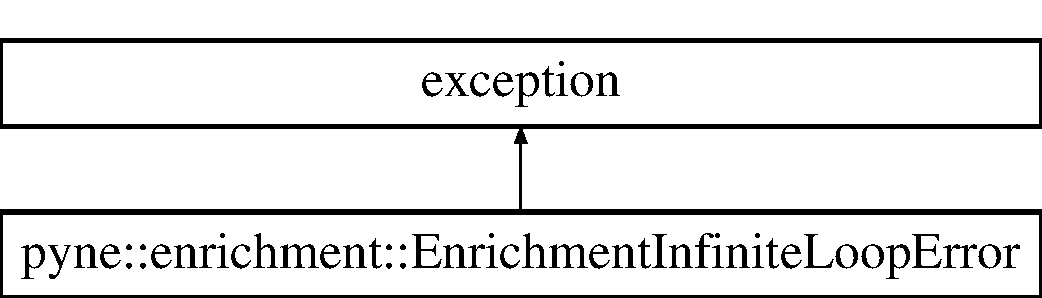
\includegraphics[height=2.000000cm]{classpyne_1_1enrichment_1_1_enrichment_infinite_loop_error}
\end{center}
\end{figure}


\subsection{Detailed Description}
Custom exception for when an enrichment solver has entered an infinite loop. 

The documentation for this class was generated from the following file\-:\begin{DoxyCompactItemize}
\item 
/home/scopatz/pyne/src/\hyperlink{enrichment_8h}{enrichment.\-h}\end{DoxyCompactItemize}

\hypertarget{classpyne_1_1enrichment_1_1_enrichment_iteration_limit}{\section{pyne\+:\+:enrichment\+:\+:Enrichment\+Iteration\+Limit Class Reference}
\label{classpyne_1_1enrichment_1_1_enrichment_iteration_limit}\index{pyne\+::enrichment\+::\+Enrichment\+Iteration\+Limit@{pyne\+::enrichment\+::\+Enrichment\+Iteration\+Limit}}
}


{\ttfamily \#include $<$enrichment.\+h$>$}

Inheritance diagram for pyne\+:\+:enrichment\+:\+:Enrichment\+Iteration\+Limit\+:\begin{figure}[H]
\begin{center}
\leavevmode
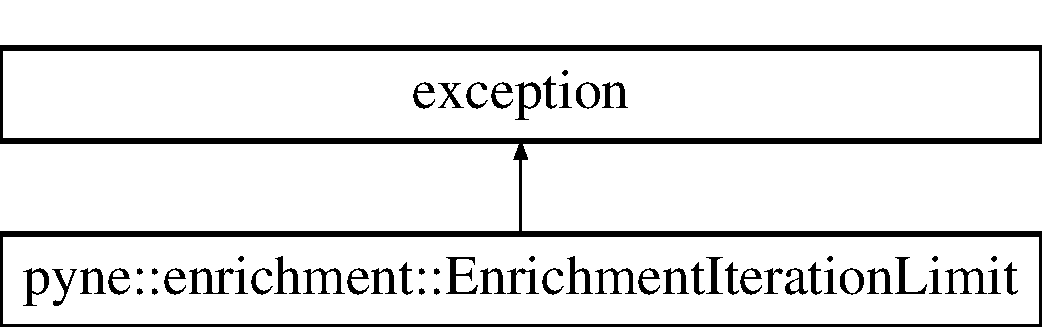
\includegraphics[height=2.000000cm]{classpyne_1_1enrichment_1_1_enrichment_iteration_limit}
\end{center}
\end{figure}


\subsection{Detailed Description}
Custom exception for when an enrichment solver has reached its maximum number of iterations. 

The documentation for this class was generated from the following file\+:\begin{DoxyCompactItemize}
\item 
/\+Users/bates26/\+Documents/pyne/src/\hyperlink{enrichment_8h}{enrichment.\+h}\end{DoxyCompactItemize}

\hypertarget{classpyne_1_1enrichment_1_1_enrichment_iteration_na_n}{\section{pyne\-:\-:enrichment\-:\-:Enrichment\-Iteration\-Na\-N Class Reference}
\label{classpyne_1_1enrichment_1_1_enrichment_iteration_na_n}\index{pyne\-::enrichment\-::\-Enrichment\-Iteration\-Na\-N@{pyne\-::enrichment\-::\-Enrichment\-Iteration\-Na\-N}}
}


Custom exception for when an enrichment solver iteration has produced a Na\-N.  




{\ttfamily \#include $<$enrichment.\-h$>$}

Inheritance diagram for pyne\-:\-:enrichment\-:\-:Enrichment\-Iteration\-Na\-N\-:\begin{figure}[H]
\begin{center}
\leavevmode
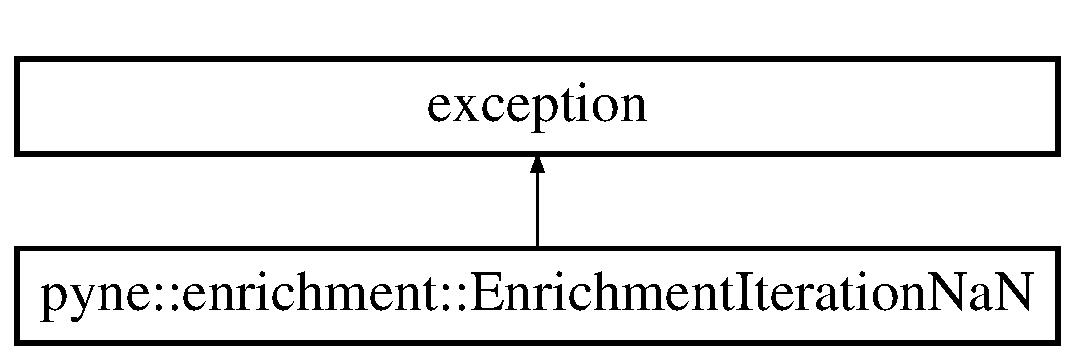
\includegraphics[height=2.000000cm]{classpyne_1_1enrichment_1_1_enrichment_iteration_na_n}
\end{center}
\end{figure}


\subsection{Detailed Description}
Custom exception for when an enrichment solver iteration has produced a Na\-N. 

The documentation for this class was generated from the following file\-:\begin{DoxyCompactItemize}
\item 
/home/elliott/\-Research/pyne/src/\hyperlink{enrichment_8h}{enrichment.\-h}\end{DoxyCompactItemize}

\hypertarget{classpyne_1_1_file_not_found}{\section{pyne\-:\-:File\-Not\-Found Class Reference}
\label{classpyne_1_1_file_not_found}\index{pyne\-::\-File\-Not\-Found@{pyne\-::\-File\-Not\-Found}}
}


{\ttfamily \#include $<$utils.\-h$>$}

Inheritance diagram for pyne\-:\-:File\-Not\-Found\-:\begin{figure}[H]
\begin{center}
\leavevmode
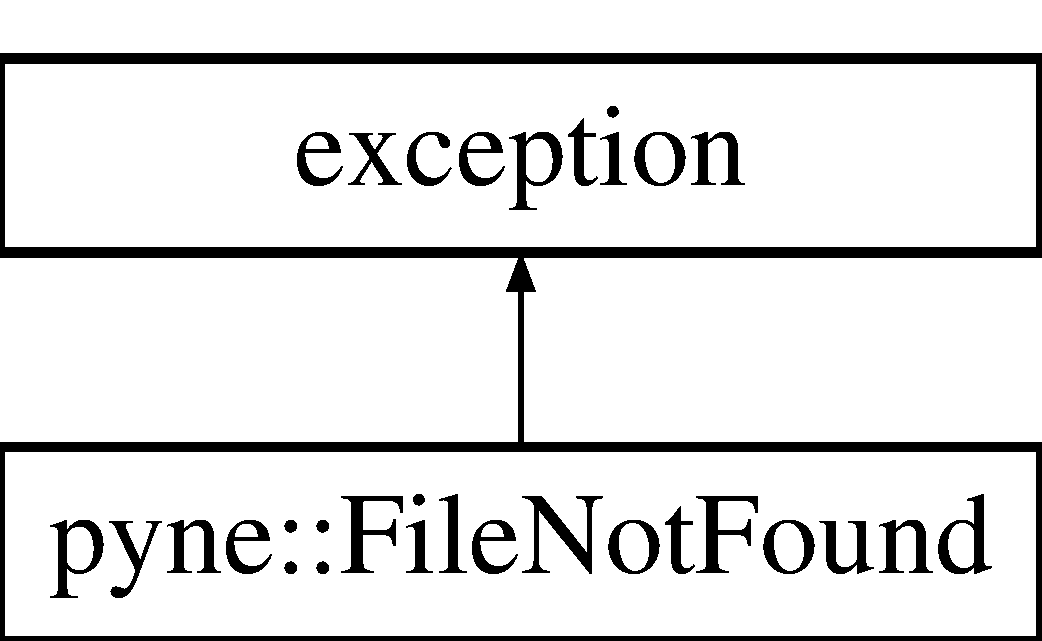
\includegraphics[height=2.000000cm]{classpyne_1_1_file_not_found}
\end{center}
\end{figure}
\subsection*{Public Member Functions}
\begin{DoxyCompactItemize}
\item 
\hypertarget{classpyne_1_1_file_not_found_aaae1bdf04df2b68377ae453929c8eb56}{\hyperlink{classpyne_1_1_file_not_found_aaae1bdf04df2b68377ae453929c8eb56}{File\-Not\-Found} ()}\label{classpyne_1_1_file_not_found_aaae1bdf04df2b68377ae453929c8eb56}

\begin{DoxyCompactList}\small\item\em default constructor \end{DoxyCompactList}\item 
\hypertarget{classpyne_1_1_file_not_found_abc00e9c8711bb1b1bb2dc1dfd3a98745}{\hyperlink{classpyne_1_1_file_not_found_abc00e9c8711bb1b1bb2dc1dfd3a98745}{$\sim$\-File\-Not\-Found} ()  throw ()}\label{classpyne_1_1_file_not_found_abc00e9c8711bb1b1bb2dc1dfd3a98745}

\begin{DoxyCompactList}\small\item\em default destructor \end{DoxyCompactList}\item 
\hypertarget{classpyne_1_1_file_not_found_a4d766115c01634b77aebe42269f9aead}{\hyperlink{classpyne_1_1_file_not_found_a4d766115c01634b77aebe42269f9aead}{File\-Not\-Found} (std\-::string fname)}\label{classpyne_1_1_file_not_found_a4d766115c01634b77aebe42269f9aead}

\begin{DoxyCompactList}\small\item\em constructor with the filename {\itshape fname}. \end{DoxyCompactList}\item 
\hypertarget{classpyne_1_1_file_not_found_a55d410139d5853e8988d073637845cbd}{virtual const char $\ast$ \hyperlink{classpyne_1_1_file_not_found_a55d410139d5853e8988d073637845cbd}{what} () const   throw ()}\label{classpyne_1_1_file_not_found_a55d410139d5853e8988d073637845cbd}

\begin{DoxyCompactList}\small\item\em Creates a helpful error message. \end{DoxyCompactList}\end{DoxyCompactItemize}


\subsection{Detailed Description}
Custom exception to be thrown in the event that a required file is not able to be found. 

The documentation for this class was generated from the following file\-:\begin{DoxyCompactItemize}
\item 
/home/scopatz/pyne/src/utils.\-h\end{DoxyCompactItemize}

\hypertarget{classh5wrap_1_1_file_not_h_d_f5}{\section{h5wrap\+:\+:File\+Not\+H\+D\+F5 Class Reference}
\label{classh5wrap_1_1_file_not_h_d_f5}\index{h5wrap\+::\+File\+Not\+H\+D\+F5@{h5wrap\+::\+File\+Not\+H\+D\+F5}}
}


Custom exception for when an existing file is not in a valid H\+D\+F5 format.  




{\ttfamily \#include $<$h5wrap.\+h$>$}

Inheritance diagram for h5wrap\+:\+:File\+Not\+H\+D\+F5\+:\begin{figure}[H]
\begin{center}
\leavevmode
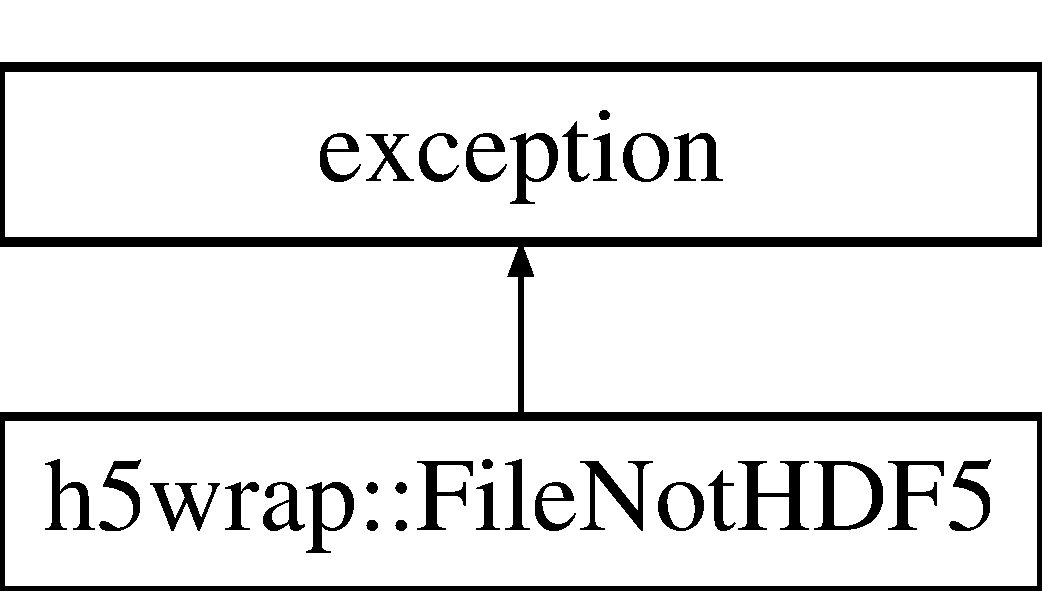
\includegraphics[height=2.000000cm]{classh5wrap_1_1_file_not_h_d_f5}
\end{center}
\end{figure}
\subsection*{Public Member Functions}
\begin{DoxyCompactItemize}
\item 
\hypertarget{classh5wrap_1_1_file_not_h_d_f5_a3fa40cb39abaa241e80ee97a13e69815}{\hyperlink{classh5wrap_1_1_file_not_h_d_f5_a3fa40cb39abaa241e80ee97a13e69815}{File\+Not\+H\+D\+F5} ()}\label{classh5wrap_1_1_file_not_h_d_f5_a3fa40cb39abaa241e80ee97a13e69815}

\begin{DoxyCompactList}\small\item\em default constructor \end{DoxyCompactList}\item 
\hypertarget{classh5wrap_1_1_file_not_h_d_f5_a55276b2bc97da82f25a0718327b00742}{\hyperlink{classh5wrap_1_1_file_not_h_d_f5_a55276b2bc97da82f25a0718327b00742}{$\sim$\+File\+Not\+H\+D\+F5} ()  throw ()}\label{classh5wrap_1_1_file_not_h_d_f5_a55276b2bc97da82f25a0718327b00742}

\begin{DoxyCompactList}\small\item\em default destructor \end{DoxyCompactList}\item 
\hypertarget{classh5wrap_1_1_file_not_h_d_f5_ac6f9e6588f3a55f26fe6cd13ab75425b}{\hyperlink{classh5wrap_1_1_file_not_h_d_f5_ac6f9e6588f3a55f26fe6cd13ab75425b}{File\+Not\+H\+D\+F5} (std\+::string fname)}\label{classh5wrap_1_1_file_not_h_d_f5_ac6f9e6588f3a55f26fe6cd13ab75425b}

\begin{DoxyCompactList}\small\item\em constructor with the filename \end{DoxyCompactList}\item 
\hypertarget{classh5wrap_1_1_file_not_h_d_f5_afce2273e3c8d54802598bdc30cdedec2}{virtual const char $\ast$ \hyperlink{classh5wrap_1_1_file_not_h_d_f5_afce2273e3c8d54802598bdc30cdedec2}{what} () const   throw ()}\label{classh5wrap_1_1_file_not_h_d_f5_afce2273e3c8d54802598bdc30cdedec2}

\begin{DoxyCompactList}\small\item\em helpful error message that includes the filename \end{DoxyCompactList}\end{DoxyCompactItemize}


\subsection{Detailed Description}
Custom exception for when an existing file is not in a valid H\+D\+F5 format. 

The documentation for this class was generated from the following file\+:\begin{DoxyCompactItemize}
\item 
/\+Users/bates26/\+Documents/pyne/src/\hyperlink{h5wrap_8h}{h5wrap.\+h}\end{DoxyCompactItemize}

\hypertarget{structpyne_1_1gamma}{\section{pyne\+:\+:gamma Struct Reference}
\label{structpyne_1_1gamma}\index{pyne\+::gamma@{pyne\+::gamma}}
}


a struct matching the '/decay/gammas' table in nuc\+\_\+data.\+h5.  




{\ttfamily \#include $<$data.\+h$>$}

\subsection*{Public Attributes}
\begin{DoxyCompactItemize}
\item 
\hypertarget{structpyne_1_1gamma_a1c5b7ef9f75c628193a0872c9ae172e4}{int \hyperlink{structpyne_1_1gamma_a1c5b7ef9f75c628193a0872c9ae172e4}{from\+\_\+nuc}}\label{structpyne_1_1gamma_a1c5b7ef9f75c628193a0872c9ae172e4}

\begin{DoxyCompactList}\small\item\em state id of starting level \end{DoxyCompactList}\item 
\hypertarget{structpyne_1_1gamma_af9ed390289a667c82464c859dbccb0a4}{int \hyperlink{structpyne_1_1gamma_af9ed390289a667c82464c859dbccb0a4}{to\+\_\+nuc}}\label{structpyne_1_1gamma_af9ed390289a667c82464c859dbccb0a4}

\begin{DoxyCompactList}\small\item\em state id of final level \end{DoxyCompactList}\item 
\hypertarget{structpyne_1_1gamma_a947386fa2557f57cc14f79d6904185bd}{int \hyperlink{structpyne_1_1gamma_a947386fa2557f57cc14f79d6904185bd}{parent\+\_\+nuc}}\label{structpyne_1_1gamma_a947386fa2557f57cc14f79d6904185bd}

\begin{DoxyCompactList}\small\item\em state id of the primary decaying nucleus \end{DoxyCompactList}\item 
\hypertarget{structpyne_1_1gamma_a99fcb3ccd78db851f7104ff3ab59048d}{int \hyperlink{structpyne_1_1gamma_a99fcb3ccd78db851f7104ff3ab59048d}{child\+\_\+nuc}}\label{structpyne_1_1gamma_a99fcb3ccd78db851f7104ff3ab59048d}

\begin{DoxyCompactList}\small\item\em stateless id of the child nucleus \end{DoxyCompactList}\item 
\hypertarget{structpyne_1_1gamma_a82e14610a750a9c31c6976c2685c223f}{double \hyperlink{structpyne_1_1gamma_a82e14610a750a9c31c6976c2685c223f}{energy}}\label{structpyne_1_1gamma_a82e14610a750a9c31c6976c2685c223f}

\begin{DoxyCompactList}\small\item\em energy of the photon \mbox{[}ke\+V\mbox{]} \end{DoxyCompactList}\item 
\hypertarget{structpyne_1_1gamma_a9682d9995810db3b59d27138c24e223a}{double \hyperlink{structpyne_1_1gamma_a9682d9995810db3b59d27138c24e223a}{energy\+\_\+err}}\label{structpyne_1_1gamma_a9682d9995810db3b59d27138c24e223a}

\begin{DoxyCompactList}\small\item\em energy error of the photon \mbox{[}ke\+V\mbox{]} \end{DoxyCompactList}\item 
\hypertarget{structpyne_1_1gamma_a5d7ca7cc0667ebc41b8f046739c0dc1b}{double \hyperlink{structpyne_1_1gamma_a5d7ca7cc0667ebc41b8f046739c0dc1b}{photon\+\_\+intensity}}\label{structpyne_1_1gamma_a5d7ca7cc0667ebc41b8f046739c0dc1b}

\begin{DoxyCompactList}\small\item\em photon intensity \end{DoxyCompactList}\item 
\hypertarget{structpyne_1_1gamma_a38f1045e9df163a740c657ca6cac490b}{double \hyperlink{structpyne_1_1gamma_a38f1045e9df163a740c657ca6cac490b}{photon\+\_\+intensity\+\_\+err}}\label{structpyne_1_1gamma_a38f1045e9df163a740c657ca6cac490b}

\begin{DoxyCompactList}\small\item\em photon intensity error \end{DoxyCompactList}\item 
\hypertarget{structpyne_1_1gamma_a6d347a0a5cfcf0765476d618b2faa71f}{double \hyperlink{structpyne_1_1gamma_a6d347a0a5cfcf0765476d618b2faa71f}{conv\+\_\+intensity}}\label{structpyne_1_1gamma_a6d347a0a5cfcf0765476d618b2faa71f}

\begin{DoxyCompactList}\small\item\em conversion intensity \end{DoxyCompactList}\item 
\hypertarget{structpyne_1_1gamma_a48c4d772b76640e6cd77805278241657}{double \hyperlink{structpyne_1_1gamma_a48c4d772b76640e6cd77805278241657}{conv\+\_\+intensity\+\_\+err}}\label{structpyne_1_1gamma_a48c4d772b76640e6cd77805278241657}

\begin{DoxyCompactList}\small\item\em conversion intensity error \end{DoxyCompactList}\item 
\hypertarget{structpyne_1_1gamma_a5d409f6a09142b6cc871158cff7d5fe7}{double \hyperlink{structpyne_1_1gamma_a5d409f6a09142b6cc871158cff7d5fe7}{total\+\_\+intensity}}\label{structpyne_1_1gamma_a5d409f6a09142b6cc871158cff7d5fe7}

\begin{DoxyCompactList}\small\item\em total decay intensity \end{DoxyCompactList}\item 
\hypertarget{structpyne_1_1gamma_a8c626cfbe36afddfadf664f2aff19f2f}{double \hyperlink{structpyne_1_1gamma_a8c626cfbe36afddfadf664f2aff19f2f}{total\+\_\+intensity\+\_\+err}}\label{structpyne_1_1gamma_a8c626cfbe36afddfadf664f2aff19f2f}

\begin{DoxyCompactList}\small\item\em total decay intensity error \end{DoxyCompactList}\item 
\hypertarget{structpyne_1_1gamma_a9b4256e35bdd191c7a6c27835642e353}{double \hyperlink{structpyne_1_1gamma_a9b4256e35bdd191c7a6c27835642e353}{k\+\_\+conv\+\_\+e}}\label{structpyne_1_1gamma_a9b4256e35bdd191c7a6c27835642e353}

\begin{DoxyCompactList}\small\item\em k conversion electron fraction \end{DoxyCompactList}\item 
\hypertarget{structpyne_1_1gamma_a9fbb2fdf8a1c5b7430afa34237509abe}{double \hyperlink{structpyne_1_1gamma_a9fbb2fdf8a1c5b7430afa34237509abe}{l\+\_\+conv\+\_\+e}}\label{structpyne_1_1gamma_a9fbb2fdf8a1c5b7430afa34237509abe}

\begin{DoxyCompactList}\small\item\em l conversion electron fraction \end{DoxyCompactList}\item 
\hypertarget{structpyne_1_1gamma_a6c664717050818947e2e79d75e914c41}{double \hyperlink{structpyne_1_1gamma_a6c664717050818947e2e79d75e914c41}{m\+\_\+conv\+\_\+e}}\label{structpyne_1_1gamma_a6c664717050818947e2e79d75e914c41}

\begin{DoxyCompactList}\small\item\em m conversion electron fraction \end{DoxyCompactList}\end{DoxyCompactItemize}


\subsection{Detailed Description}
a struct matching the '/decay/gammas' table in nuc\+\_\+data.\+h5. 

The documentation for this struct was generated from the following file\+:\begin{DoxyCompactItemize}
\item 
/\+Users/bates26/\+Documents/pyne/src/\hyperlink{data_8h}{data.\+h}\end{DoxyCompactItemize}

\hypertarget{classgeompack}{\section{geompack Module Reference}
\label{classgeompack}\index{geompack@{geompack}}
}
\subsection*{Public Member Functions}
\begin{DoxyCompactItemize}
\item 
\hypertarget{classgeompack_a2317ab8af14e0fa670245b6d67ed7b60}{integer(kind=4) function {\bfseries opside} (a, b, c, d, e)}\label{classgeompack_a2317ab8af14e0fa670245b6d67ed7b60}

\item 
\hypertarget{classgeompack_a6285805baeace70de928605567d0ea99}{subroutine {\bfseries dtris3} (npt, sizht, bf\+\_\+max, fc\+\_\+max, vcl, vm, bf\+\_\+num, nfc, nface, ntetra, bf, fc, ht, ierr)}\label{classgeompack_a6285805baeace70de928605567d0ea99}

\item 
\hypertarget{classgeompack_a7a0dea21fde829963eb4ef699df1cafc}{subroutine {\bfseries dhpsrt} (k, n, lda, a, map)}\label{classgeompack_a7a0dea21fde829963eb4ef699df1cafc}

\item 
\hypertarget{classgeompack_a23717a1d896374a24d14b4ca0c792e1f}{subroutine {\bfseries dsftdw} (l, u, k, lda, a, map)}\label{classgeompack_a23717a1d896374a24d14b4ca0c792e1f}

\item 
\hypertarget{classgeompack_a9614867a3a0edc826e6fb078cb07976c}{logical function {\bfseries dless} (k, p, q)}\label{classgeompack_a9614867a3a0edc826e6fb078cb07976c}

\item 
\hypertarget{classgeompack_a7f34140747c618d0e2392452b2e25098}{subroutine {\bfseries frstet} (shift, nv, vcl, map, i3, i4, ierr)}\label{classgeompack_a7f34140747c618d0e2392452b2e25098}

\item 
\hypertarget{classgeompack_a8719c6bd2f3f88cce35c0c64f0328926}{subroutine {\bfseries htins} (ind, a, b, c, d, e, n, p, fc, ht)}\label{classgeompack_a8719c6bd2f3f88cce35c0c64f0328926}

\item 
\hypertarget{classgeompack_ab9a0ea5a4297d18017861d316368cd3a}{subroutine {\bfseries order3} (i, j, k)}\label{classgeompack_ab9a0ea5a4297d18017861d316368cd3a}

\item 
\hypertarget{classgeompack_af761b81a1f9f1919f4fa7398294f0204}{subroutine {\bfseries i4\+\_\+swap} (i, j)}\label{classgeompack_af761b81a1f9f1919f4fa7398294f0204}

\item 
\hypertarget{classgeompack_a1c3d1834ba851e5883085a7538fac325}{subroutine {\bfseries vbfac} (pt, ctr, vcl, vm, bf, fc, topv, topnv)}\label{classgeompack_a1c3d1834ba851e5883085a7538fac325}

\item 
\hypertarget{classgeompack_a47f5b11cf75357fd64f413a95b8c3693}{subroutine {\bfseries nwthou} (i, npt, sizht, bf\+\_\+num, nfc, bf\+\_\+max, fc\+\_\+max, bf, fc, ht, ntetra, hdavbf, hdavfc, front, back, bfi, ierr)}\label{classgeompack_a47f5b11cf75357fd64f413a95b8c3693}

\item 
\hypertarget{classgeompack_ab9776020bebd9214113f936bcad52730}{subroutine {\bfseries swapes} (bndcon, i, npt, sizht, fc\+\_\+num, fc\+\_\+max, vcl, vm, bf, fc, ht, ntetra, hdavfc, front, back, ifac, ierr)}\label{classgeompack_ab9776020bebd9214113f936bcad52730}

\item 
\hypertarget{classgeompack_aad03504a4ad7580a4ce1f95e531fc192}{subroutine {\bfseries ccsph} (intest, a, b, c, d, e, center, radsq, in)}\label{classgeompack_aad03504a4ad7580a4ce1f95e531fc192}

\item 
\hypertarget{classgeompack_a5aa5b559af437154aad3f2244f5d8177}{subroutine {\bfseries baryth} (a, b, c, d, e, alpha, degen)}\label{classgeompack_a5aa5b559af437154aad3f2244f5d8177}

\item 
\hypertarget{classgeompack_a94821d7a86962c544c59783cbbe47741}{subroutine {\bfseries updatf} (a, b, c, d, e, i, n, p, front, back, fc, ht, ierr)}\label{classgeompack_a94821d7a86962c544c59783cbbe47741}

\item 
\hypertarget{classgeompack_a1b15210098b4ac9ad8f4455b58440b82}{subroutine {\bfseries htdel} (ind, n, p, fc, ht)}\label{classgeompack_a1b15210098b4ac9ad8f4455b58440b82}

\item 
\hypertarget{classgeompack_a1393b15dd71c58b324712b49d7b1b6e5}{subroutine {\bfseries availf} (hdavfc, fc\+\_\+num, fc\+\_\+max, fc, ind, ierr)}\label{classgeompack_a1393b15dd71c58b324712b49d7b1b6e5}

\item 
\hypertarget{classgeompack_ac0a055d7534043b545b23cb09104b68e}{integer(kind=4) function {\bfseries htsrc} (a, b, c, n, p, fc, ht)}\label{classgeompack_ac0a055d7534043b545b23cb09104b68e}

\item 
\hypertarget{classgeompack_ac83af4943560085ee3f25b817aa45b9c}{subroutine {\bfseries dtriw2} (npt, maxst, vcl, ind, ntri, til, tnbr, stack, ierr)}\label{classgeompack_ac83af4943560085ee3f25b817aa45b9c}

\item 
\hypertarget{classgeompack_a25b0a5c22a744be77665e36e4a1062af}{subroutine {\bfseries walkt2} (x, y, ntri, vcl, til, tnbr, itri, iedg, ierr)}\label{classgeompack_a25b0a5c22a744be77665e36e4a1062af}

\item 
\hypertarget{classgeompack_a38c94eee465e80bf8838faf84fbecc0c}{subroutine {\bfseries vbedg} (x, y, vcl, til, tnbr, ltri, ledg, rtri, redg)}\label{classgeompack_a38c94eee465e80bf8838faf84fbecc0c}

\item 
\hypertarget{classgeompack_a9ad84c591ca6884ed9df315f68f3f30c}{integer(kind=4) function {\bfseries lrline} (xu, yu, xv1, yv1, xv2, yv2, dv)}\label{classgeompack_a9ad84c591ca6884ed9df315f68f3f30c}

\item 
\hypertarget{classgeompack_a55066c94f489f5a120f06c1f576e167f}{subroutine {\bfseries swapec} (i, top, maxst, btri, bedg, vcl, til, tnbr, stack, ierr)}\label{classgeompack_a55066c94f489f5a120f06c1f576e167f}

\item 
\hypertarget{classgeompack_aa309a784a534b06779c17338510e1d7e}{integer(kind=4) function {\bfseries diaedg} (x0, y0, x1, y1, x2, y2, x3, y3)}\label{classgeompack_aa309a784a534b06779c17338510e1d7e}

\item 
\hypertarget{classgeompack_a4ea8209ecfbd40ef48d79302d930352f}{subroutine {\bfseries tetlst} (nfc, vm, fc, nt, tetra)}\label{classgeompack_a4ea8209ecfbd40ef48d79302d930352f}

\item 
\hypertarget{classgeompack_ac332e0faf391cc194c70cfc300de1059}{subroutine {\bfseries baryck} (k, ind, vcl, pt, alpha, degen, mat, ipvt)}\label{classgeompack_ac332e0faf391cc194c70cfc300de1059}

\item 
\hypertarget{classgeompack_aa3c5e87b0e2e939bb490bb9591939213}{subroutine {\bfseries lufac} (a, lda, n, tol, ipvt, singlr)}\label{classgeompack_aa3c5e87b0e2e939bb490bb9591939213}

\item 
\hypertarget{classgeompack_a4b68a0623aa709973fa045f833408ce4}{subroutine {\bfseries lusol} (a, lda, n, ipvt, b)}\label{classgeompack_a4b68a0623aa709973fa045f833408ce4}

\end{DoxyCompactItemize}


The documentation for this module was generated from the following file\+:\begin{DoxyCompactItemize}
\item 
/\+Users/bates26/\+Documents/pyne/src/ahot/spatial\+\_\+solvers\+\_\+3d/\+S\+C\+T-\/\+Step/src\+\_\+ahotn-\/step-\/sct/geompack.\+f90\end{DoxyCompactItemize}

\hypertarget{classh5wrap_1_1_group_not_found}{\section{h5wrap\+:\+:Group\+Not\+Found Class Reference}
\label{classh5wrap_1_1_group_not_found}\index{h5wrap\+::\+Group\+Not\+Found@{h5wrap\+::\+Group\+Not\+Found}}
}


Custom exception for when a group cannot be found in an H\+D\+F5 file.  




{\ttfamily \#include $<$h5wrap.\+h$>$}

Inheritance diagram for h5wrap\+:\+:Group\+Not\+Found\+:\begin{figure}[H]
\begin{center}
\leavevmode
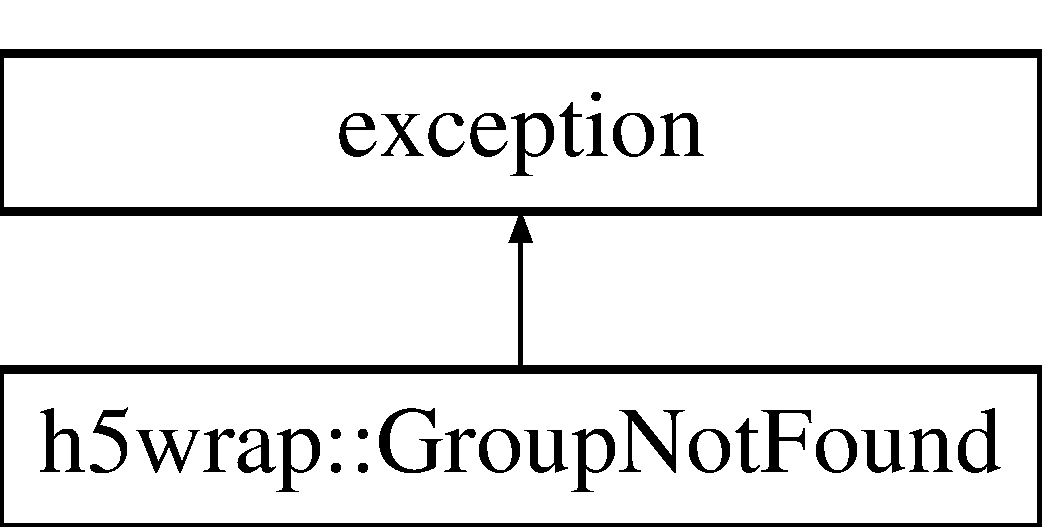
\includegraphics[height=2.000000cm]{classh5wrap_1_1_group_not_found}
\end{center}
\end{figure}
\subsection*{Public Member Functions}
\begin{DoxyCompactItemize}
\item 
\hypertarget{classh5wrap_1_1_group_not_found_accc7d7bea9e86968335a46ee39d7d543}{\hyperlink{classh5wrap_1_1_group_not_found_accc7d7bea9e86968335a46ee39d7d543}{Group\+Not\+Found} ()}\label{classh5wrap_1_1_group_not_found_accc7d7bea9e86968335a46ee39d7d543}

\begin{DoxyCompactList}\small\item\em default constructor \end{DoxyCompactList}\item 
\hypertarget{classh5wrap_1_1_group_not_found_a79dea7d1d5e3ffd7a7e83b4a2636398a}{\hyperlink{classh5wrap_1_1_group_not_found_a79dea7d1d5e3ffd7a7e83b4a2636398a}{$\sim$\+Group\+Not\+Found} ()  throw ()}\label{classh5wrap_1_1_group_not_found_a79dea7d1d5e3ffd7a7e83b4a2636398a}

\begin{DoxyCompactList}\small\item\em default destructor \end{DoxyCompactList}\item 
\hypertarget{classh5wrap_1_1_group_not_found_a74f7e8f6efcf33503f5fec62eead40c3}{\hyperlink{classh5wrap_1_1_group_not_found_a74f7e8f6efcf33503f5fec62eead40c3}{Group\+Not\+Found} (std\+::string fname, std\+::string gname)}\label{classh5wrap_1_1_group_not_found_a74f7e8f6efcf33503f5fec62eead40c3}

\begin{DoxyCompactList}\small\item\em constructor with the filename and the groupname \end{DoxyCompactList}\item 
\hypertarget{classh5wrap_1_1_group_not_found_a76766dc5fda0a07564379db454df87d0}{virtual const char $\ast$ \hyperlink{classh5wrap_1_1_group_not_found_a76766dc5fda0a07564379db454df87d0}{what} () const   throw ()}\label{classh5wrap_1_1_group_not_found_a76766dc5fda0a07564379db454df87d0}

\begin{DoxyCompactList}\small\item\em helpful error message that includes the filename and the groupname \end{DoxyCompactList}\end{DoxyCompactItemize}


\subsection{Detailed Description}
Custom exception for when a group cannot be found in an H\+D\+F5 file. 

The documentation for this class was generated from the following file\+:\begin{DoxyCompactItemize}
\item 
/\+Users/bates26/\+Documents/pyne/src/\hyperlink{h5wrap_8h}{h5wrap.\+h}\end{DoxyCompactItemize}

\hypertarget{classh5wrap_1_1_h_d_f5_bounds_error}{\section{h5wrap\-:\-:H\-D\-F5\-Bounds\-Error Class Reference}
\label{classh5wrap_1_1_h_d_f5_bounds_error}\index{h5wrap\-::\-H\-D\-F5\-Bounds\-Error@{h5wrap\-::\-H\-D\-F5\-Bounds\-Error}}
}


Custom exception for H\-D\-F5 indexing errors.  




{\ttfamily \#include $<$h5wrap.\-h$>$}

Inheritance diagram for h5wrap\-:\-:H\-D\-F5\-Bounds\-Error\-:\begin{figure}[H]
\begin{center}
\leavevmode
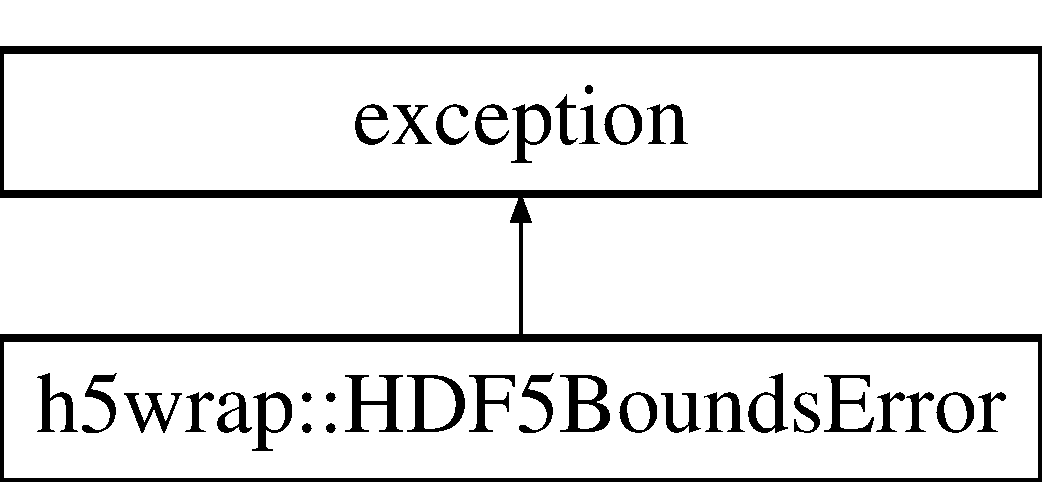
\includegraphics[height=2.000000cm]{classh5wrap_1_1_h_d_f5_bounds_error}
\end{center}
\end{figure}


\subsection{Detailed Description}
Custom exception for H\-D\-F5 indexing errors. 

The documentation for this class was generated from the following file\-:\begin{DoxyCompactItemize}
\item 
/home/elliott/\-Research/pyne/src/\hyperlink{h5wrap_8h}{h5wrap.\-h}\end{DoxyCompactItemize}

\hypertarget{classh5wrap_1_1_homogenous_type_table}{\section{h5wrap\-:\-:Homogenous\-Type\-Table$<$ T $>$ Class Template Reference}
\label{classh5wrap_1_1_homogenous_type_table}\index{h5wrap\-::\-Homogenous\-Type\-Table$<$ T $>$@{h5wrap\-::\-Homogenous\-Type\-Table$<$ T $>$}}
}


{\ttfamily \#include $<$h5wrap.\-h$>$}

\subsection*{Public Member Functions}
\begin{DoxyCompactItemize}
\item 
\hypertarget{classh5wrap_1_1_homogenous_type_table_a4abe000d3595d0ff78354bc5131b1ca7}{\hyperlink{classh5wrap_1_1_homogenous_type_table_a4abe000d3595d0ff78354bc5131b1ca7}{Homogenous\-Type\-Table} ()}\label{classh5wrap_1_1_homogenous_type_table_a4abe000d3595d0ff78354bc5131b1ca7}

\begin{DoxyCompactList}\small\item\em default constructor \end{DoxyCompactList}\item 
\hypertarget{classh5wrap_1_1_homogenous_type_table_aa339bef26857f755e42035d4e054d7c7}{\hyperlink{classh5wrap_1_1_homogenous_type_table_aa339bef26857f755e42035d4e054d7c7}{$\sim$\-Homogenous\-Type\-Table} ()}\label{classh5wrap_1_1_homogenous_type_table_aa339bef26857f755e42035d4e054d7c7}

\begin{DoxyCompactList}\small\item\em default destructor \end{DoxyCompactList}\item 
\hyperlink{classh5wrap_1_1_homogenous_type_table_a2fd7306656d5a16b4a44b50a9271eab3}{Homogenous\-Type\-Table} (hid\-\_\-t h5file, std\-::string data\-\_\-path, hid\-\_\-t dtype=H5\-T\-\_\-\-N\-A\-T\-I\-V\-E\-\_\-\-D\-O\-U\-B\-L\-E)
\item 
\hypertarget{classh5wrap_1_1_homogenous_type_table_a961e0edb817f203b00367202d3c278b4}{std\-::vector$<$ T $>$ \hyperlink{classh5wrap_1_1_homogenous_type_table_a961e0edb817f203b00367202d3c278b4}{operator\mbox{[}$\,$\mbox{]}} (std\-::string col\-\_\-name)}\label{classh5wrap_1_1_homogenous_type_table_a961e0edb817f203b00367202d3c278b4}

\begin{DoxyCompactList}\small\item\em index into the table by column name (string) \end{DoxyCompactList}\item 
\hypertarget{classh5wrap_1_1_homogenous_type_table_a777f6bdc03111b5a7d8fde59e184e26c}{std\-::map$<$ std\-::string, T $>$ \hyperlink{classh5wrap_1_1_homogenous_type_table_a777f6bdc03111b5a7d8fde59e184e26c}{operator\mbox{[}$\,$\mbox{]}} (int m)}\label{classh5wrap_1_1_homogenous_type_table_a777f6bdc03111b5a7d8fde59e184e26c}

\begin{DoxyCompactList}\small\item\em index into the table by row \end{DoxyCompactList}\end{DoxyCompactItemize}
\subsection*{Public Attributes}
\begin{DoxyCompactItemize}
\item 
\hypertarget{classh5wrap_1_1_homogenous_type_table_a6da460e4b94719f9ff5fe0d17e8859d7}{std\-::string \hyperlink{classh5wrap_1_1_homogenous_type_table_a6da460e4b94719f9ff5fe0d17e8859d7}{path}}\label{classh5wrap_1_1_homogenous_type_table_a6da460e4b94719f9ff5fe0d17e8859d7}

\begin{DoxyCompactList}\small\item\em path in file to the data \end{DoxyCompactList}\item 
\hypertarget{classh5wrap_1_1_homogenous_type_table_ab0e03ddbee134e775ea6fa389897fc8b}{int \hyperlink{classh5wrap_1_1_homogenous_type_table_ab0e03ddbee134e775ea6fa389897fc8b}{shape} \mbox{[}2\mbox{]}}\label{classh5wrap_1_1_homogenous_type_table_ab0e03ddbee134e775ea6fa389897fc8b}

\begin{DoxyCompactList}\small\item\em table shape, rows x columns. \end{DoxyCompactList}\item 
std\-::vector$<$ std\-::string $>$ \hyperlink{classh5wrap_1_1_homogenous_type_table_a8b60fa54475f44bea26caab0137d8507}{cols}
\item 
\hypertarget{classh5wrap_1_1_homogenous_type_table_a06c1889b5469abf303923b17b78a381b}{std\-::map$<$ std\-::string, \\*
std\-::vector$<$ T $>$ $>$ \hyperlink{classh5wrap_1_1_homogenous_type_table_a06c1889b5469abf303923b17b78a381b}{data}}\label{classh5wrap_1_1_homogenous_type_table_a06c1889b5469abf303923b17b78a381b}

\begin{DoxyCompactList}\small\item\em mapping from column names to column data \end{DoxyCompactList}\end{DoxyCompactItemize}


\subsection{Detailed Description}
\subsubsection*{template$<$typename T$>$class h5wrap\-::\-Homogenous\-Type\-Table$<$ T $>$}

A class representing a high-\/level table contruct whose columns all have the same type {\itshape T} in C/\-C++ (and the analogous type in H\-D\-F5). 

\subsection{Constructor \& Destructor Documentation}
\hypertarget{classh5wrap_1_1_homogenous_type_table_a2fd7306656d5a16b4a44b50a9271eab3}{\index{h5wrap\-::\-Homogenous\-Type\-Table@{h5wrap\-::\-Homogenous\-Type\-Table}!Homogenous\-Type\-Table@{Homogenous\-Type\-Table}}
\index{Homogenous\-Type\-Table@{Homogenous\-Type\-Table}!h5wrap::HomogenousTypeTable@{h5wrap\-::\-Homogenous\-Type\-Table}}
\subsubsection[{Homogenous\-Type\-Table}]{\setlength{\rightskip}{0pt plus 5cm}template$<$typename T $>$ {\bf h5wrap\-::\-Homogenous\-Type\-Table}$<$ T $>$\-::{\bf Homogenous\-Type\-Table} (
\begin{DoxyParamCaption}
\item[{hid\-\_\-t}]{h5file, }
\item[{std\-::string}]{data\-\_\-path, }
\item[{hid\-\_\-t}]{dtype = {\ttfamily H5T\-\_\-NATIVE\-\_\-DOUBLE}}
\end{DoxyParamCaption}
)\hspace{0.3cm}{\ttfamily [inline]}}}\label{classh5wrap_1_1_homogenous_type_table_a2fd7306656d5a16b4a44b50a9271eab3}
Constructor to load in data upon initialization. {\itshape T} should roughly match {\itshape dtype}. 
\begin{DoxyParams}{Parameters}
{\em h5file} & H\-D\-F5 file id for an open file. \\
\hline
{\em data\-\_\-path} & path to the data in the open file. \\
\hline
{\em dtype} & H\-D\-F5 data type for the data set at {\itshape data\-\_\-path}. \\
\hline
\end{DoxyParams}


\subsection{Member Data Documentation}
\hypertarget{classh5wrap_1_1_homogenous_type_table_a8b60fa54475f44bea26caab0137d8507}{\index{h5wrap\-::\-Homogenous\-Type\-Table@{h5wrap\-::\-Homogenous\-Type\-Table}!cols@{cols}}
\index{cols@{cols}!h5wrap::HomogenousTypeTable@{h5wrap\-::\-Homogenous\-Type\-Table}}
\subsubsection[{cols}]{\setlength{\rightskip}{0pt plus 5cm}template$<$typename T $>$ std\-::vector$<$std\-::string$>$ {\bf h5wrap\-::\-Homogenous\-Type\-Table}$<$ T $>$\-::cols}}\label{classh5wrap_1_1_homogenous_type_table_a8b60fa54475f44bea26caab0137d8507}
column names 

The documentation for this class was generated from the following file\-:\begin{DoxyCompactItemize}
\item 
/home/scopatz/pyne/src/\hyperlink{h5wrap_8h}{h5wrap.\-h}\end{DoxyCompactItemize}

\hypertarget{classigeompack}{\section{igeompack Module Reference}
\label{classigeompack}\index{igeompack@{igeompack}}
}
\subsection*{Public Member Functions}
\begin{DoxyCompactItemize}
\item 
\hypertarget{classigeompack_af1c735d960955c236182dc083e4e9840}{subroutine {\bfseries idelaunay2d} (npt, vcl, ntri, tri)}\label{classigeompack_af1c735d960955c236182dc083e4e9840}

\item 
\hypertarget{classigeompack_a5afd38aaf62a7dc9d576f59edb07ef93}{subroutine {\bfseries idelaunay} (npt, vcl, nsmplx, smplx)}\label{classigeompack_a5afd38aaf62a7dc9d576f59edb07ef93}

\end{DoxyCompactItemize}


The documentation for this module was generated from the following file\-:\begin{DoxyCompactItemize}
\item 
/home/scopatz/pyne/src/ahot/spatial\-\_\-solvers\-\_\-3d/\-S\-C\-T-\/\-Step/src\-\_\-ahotn-\/step-\/sct/igeompack.\-f90\end{DoxyCompactItemize}

\hypertarget{classpyne_1_1nucname_1_1_indeterminate_nuclide_form}{\section{pyne\+:\+:nucname\+:\+:Indeterminate\+Nuclide\+Form Class Reference}
\label{classpyne_1_1nucname_1_1_indeterminate_nuclide_form}\index{pyne\+::nucname\+::\+Indeterminate\+Nuclide\+Form@{pyne\+::nucname\+::\+Indeterminate\+Nuclide\+Form}}
}


{\ttfamily \#include $<$nucname.\+h$>$}

Inheritance diagram for pyne\+:\+:nucname\+:\+:Indeterminate\+Nuclide\+Form\+:\begin{figure}[H]
\begin{center}
\leavevmode
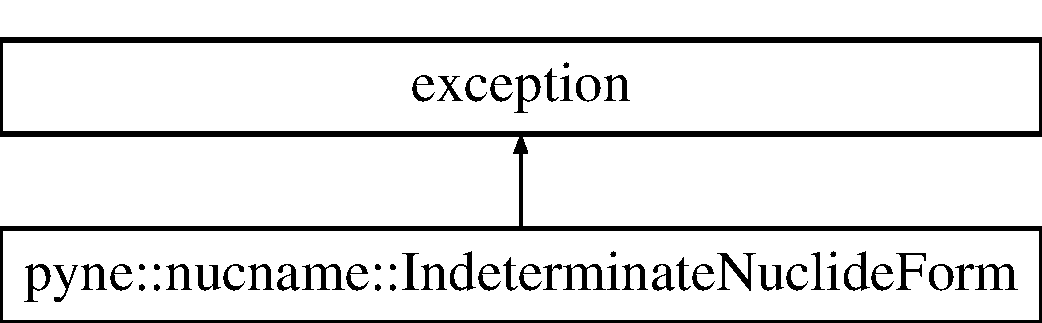
\includegraphics[height=2.000000cm]{classpyne_1_1nucname_1_1_indeterminate_nuclide_form}
\end{center}
\end{figure}
\subsection*{Public Member Functions}
\begin{DoxyCompactItemize}
\item 
\hypertarget{classpyne_1_1nucname_1_1_indeterminate_nuclide_form_aee3a250200624d6f4ab5935fd1e13d21}{\hyperlink{classpyne_1_1nucname_1_1_indeterminate_nuclide_form_aee3a250200624d6f4ab5935fd1e13d21}{Indeterminate\+Nuclide\+Form} ()}\label{classpyne_1_1nucname_1_1_indeterminate_nuclide_form_aee3a250200624d6f4ab5935fd1e13d21}

\begin{DoxyCompactList}\small\item\em default constructor \end{DoxyCompactList}\item 
\hypertarget{classpyne_1_1nucname_1_1_indeterminate_nuclide_form_afc4bbaae82a451dcbf3a85b62ab8de0e}{\hyperlink{classpyne_1_1nucname_1_1_indeterminate_nuclide_form_afc4bbaae82a451dcbf3a85b62ab8de0e}{$\sim$\+Indeterminate\+Nuclide\+Form} ()  throw ()}\label{classpyne_1_1nucname_1_1_indeterminate_nuclide_form_afc4bbaae82a451dcbf3a85b62ab8de0e}

\begin{DoxyCompactList}\small\item\em default destuctor \end{DoxyCompactList}\item 
\hyperlink{classpyne_1_1nucname_1_1_indeterminate_nuclide_form_a74d77801a214b679461eaf5dfbf7ab02}{Indeterminate\+Nuclide\+Form} (std\+::string wasptr, std\+::string nowptr)
\item 
\hyperlink{classpyne_1_1nucname_1_1_indeterminate_nuclide_form_a93724a9906be5a73b43b09ecdfed872d}{Indeterminate\+Nuclide\+Form} (std\+::string wasptr, int nowptr)
\item 
\hyperlink{classpyne_1_1nucname_1_1_indeterminate_nuclide_form_a3c9c6d0c859f3344fbb78b4259733678}{Indeterminate\+Nuclide\+Form} (int wasptr, std\+::string nowptr)
\item 
\hyperlink{classpyne_1_1nucname_1_1_indeterminate_nuclide_form_a565a1ca748bf437b18eee4834f65bf19}{Indeterminate\+Nuclide\+Form} (int wasptr, int nowptr)
\item 
virtual const char $\ast$ \hyperlink{classpyne_1_1nucname_1_1_indeterminate_nuclide_form_a9103205a7bd38dec5118e84508ed4bdb}{what} () const   throw ()
\end{DoxyCompactItemize}


\subsection{Detailed Description}
Custom expection for declaring that a value represents one or more nuclides in one or more namig conventions 

\subsection{Constructor \& Destructor Documentation}
\hypertarget{classpyne_1_1nucname_1_1_indeterminate_nuclide_form_a74d77801a214b679461eaf5dfbf7ab02}{\index{pyne\+::nucname\+::\+Indeterminate\+Nuclide\+Form@{pyne\+::nucname\+::\+Indeterminate\+Nuclide\+Form}!Indeterminate\+Nuclide\+Form@{Indeterminate\+Nuclide\+Form}}
\index{Indeterminate\+Nuclide\+Form@{Indeterminate\+Nuclide\+Form}!pyne\+::nucname\+::\+Indeterminate\+Nuclide\+Form@{pyne\+::nucname\+::\+Indeterminate\+Nuclide\+Form}}
\subsubsection[{Indeterminate\+Nuclide\+Form}]{\setlength{\rightskip}{0pt plus 5cm}pyne\+::nucname\+::\+Indeterminate\+Nuclide\+Form\+::\+Indeterminate\+Nuclide\+Form (
\begin{DoxyParamCaption}
\item[{std\+::string}]{wasptr, }
\item[{std\+::string}]{nowptr}
\end{DoxyParamCaption}
)\hspace{0.3cm}{\ttfamily [inline]}}}\label{classpyne_1_1nucname_1_1_indeterminate_nuclide_form_a74d77801a214b679461eaf5dfbf7ab02}
Constructor given previous and current state of nulide name 
\begin{DoxyParams}{Parameters}
{\em wasptr} & Previous state, typically user input. \\
\hline
{\em nowptr} & Current state, as far as Py\+N\+E could get. \\
\hline
\end{DoxyParams}
\hypertarget{classpyne_1_1nucname_1_1_indeterminate_nuclide_form_a93724a9906be5a73b43b09ecdfed872d}{\index{pyne\+::nucname\+::\+Indeterminate\+Nuclide\+Form@{pyne\+::nucname\+::\+Indeterminate\+Nuclide\+Form}!Indeterminate\+Nuclide\+Form@{Indeterminate\+Nuclide\+Form}}
\index{Indeterminate\+Nuclide\+Form@{Indeterminate\+Nuclide\+Form}!pyne\+::nucname\+::\+Indeterminate\+Nuclide\+Form@{pyne\+::nucname\+::\+Indeterminate\+Nuclide\+Form}}
\subsubsection[{Indeterminate\+Nuclide\+Form}]{\setlength{\rightskip}{0pt plus 5cm}pyne\+::nucname\+::\+Indeterminate\+Nuclide\+Form\+::\+Indeterminate\+Nuclide\+Form (
\begin{DoxyParamCaption}
\item[{std\+::string}]{wasptr, }
\item[{int}]{nowptr}
\end{DoxyParamCaption}
)\hspace{0.3cm}{\ttfamily [inline]}}}\label{classpyne_1_1nucname_1_1_indeterminate_nuclide_form_a93724a9906be5a73b43b09ecdfed872d}
Constructor given previous and current state of nulide name 
\begin{DoxyParams}{Parameters}
{\em wasptr} & Previous state, typically user input. \\
\hline
{\em nowptr} & Current state, as far as Py\+N\+E could get. \\
\hline
\end{DoxyParams}
\hypertarget{classpyne_1_1nucname_1_1_indeterminate_nuclide_form_a3c9c6d0c859f3344fbb78b4259733678}{\index{pyne\+::nucname\+::\+Indeterminate\+Nuclide\+Form@{pyne\+::nucname\+::\+Indeterminate\+Nuclide\+Form}!Indeterminate\+Nuclide\+Form@{Indeterminate\+Nuclide\+Form}}
\index{Indeterminate\+Nuclide\+Form@{Indeterminate\+Nuclide\+Form}!pyne\+::nucname\+::\+Indeterminate\+Nuclide\+Form@{pyne\+::nucname\+::\+Indeterminate\+Nuclide\+Form}}
\subsubsection[{Indeterminate\+Nuclide\+Form}]{\setlength{\rightskip}{0pt plus 5cm}pyne\+::nucname\+::\+Indeterminate\+Nuclide\+Form\+::\+Indeterminate\+Nuclide\+Form (
\begin{DoxyParamCaption}
\item[{int}]{wasptr, }
\item[{std\+::string}]{nowptr}
\end{DoxyParamCaption}
)\hspace{0.3cm}{\ttfamily [inline]}}}\label{classpyne_1_1nucname_1_1_indeterminate_nuclide_form_a3c9c6d0c859f3344fbb78b4259733678}
Constructor given previous and current state of nulide name 
\begin{DoxyParams}{Parameters}
{\em wasptr} & Previous state, typically user input. \\
\hline
{\em nowptr} & Current state, as far as Py\+N\+E could get. \\
\hline
\end{DoxyParams}
\hypertarget{classpyne_1_1nucname_1_1_indeterminate_nuclide_form_a565a1ca748bf437b18eee4834f65bf19}{\index{pyne\+::nucname\+::\+Indeterminate\+Nuclide\+Form@{pyne\+::nucname\+::\+Indeterminate\+Nuclide\+Form}!Indeterminate\+Nuclide\+Form@{Indeterminate\+Nuclide\+Form}}
\index{Indeterminate\+Nuclide\+Form@{Indeterminate\+Nuclide\+Form}!pyne\+::nucname\+::\+Indeterminate\+Nuclide\+Form@{pyne\+::nucname\+::\+Indeterminate\+Nuclide\+Form}}
\subsubsection[{Indeterminate\+Nuclide\+Form}]{\setlength{\rightskip}{0pt plus 5cm}pyne\+::nucname\+::\+Indeterminate\+Nuclide\+Form\+::\+Indeterminate\+Nuclide\+Form (
\begin{DoxyParamCaption}
\item[{int}]{wasptr, }
\item[{int}]{nowptr}
\end{DoxyParamCaption}
)\hspace{0.3cm}{\ttfamily [inline]}}}\label{classpyne_1_1nucname_1_1_indeterminate_nuclide_form_a565a1ca748bf437b18eee4834f65bf19}
Constructor given previous and current state of nulide name 
\begin{DoxyParams}{Parameters}
{\em wasptr} & Previous state, typically user input. \\
\hline
{\em nowptr} & Current state, as far as Py\+N\+E could get. \\
\hline
\end{DoxyParams}


\subsection{Member Function Documentation}
\hypertarget{classpyne_1_1nucname_1_1_indeterminate_nuclide_form_a9103205a7bd38dec5118e84508ed4bdb}{\index{pyne\+::nucname\+::\+Indeterminate\+Nuclide\+Form@{pyne\+::nucname\+::\+Indeterminate\+Nuclide\+Form}!what@{what}}
\index{what@{what}!pyne\+::nucname\+::\+Indeterminate\+Nuclide\+Form@{pyne\+::nucname\+::\+Indeterminate\+Nuclide\+Form}}
\subsubsection[{what}]{\setlength{\rightskip}{0pt plus 5cm}virtual const char$\ast$ pyne\+::nucname\+::\+Indeterminate\+Nuclide\+Form\+::what (
\begin{DoxyParamCaption}
{}
\end{DoxyParamCaption}
) const throw  ) \hspace{0.3cm}{\ttfamily [inline]}, {\ttfamily [virtual]}}}\label{classpyne_1_1nucname_1_1_indeterminate_nuclide_form_a9103205a7bd38dec5118e84508ed4bdb}
Generates an informational message for the exception \begin{DoxyReturn}{Returns}
The error string 
\end{DoxyReturn}


The documentation for this class was generated from the following file\+:\begin{DoxyCompactItemize}
\item 
/\+Users/bates26/\+Documents/pyne/src/nucname.\+h\end{DoxyCompactItemize}

\hypertarget{classpyne_1_1rxname_1_1_indeterminate_reaction_form}{\section{pyne\-:\-:rxname\-:\-:Indeterminate\-Reaction\-Form Class Reference}
\label{classpyne_1_1rxname_1_1_indeterminate_reaction_form}\index{pyne\-::rxname\-::\-Indeterminate\-Reaction\-Form@{pyne\-::rxname\-::\-Indeterminate\-Reaction\-Form}}
}


Custom exception for declaring a value not to be of ambiquous reaction form.  




{\ttfamily \#include $<$rxname.\-h$>$}

Inheritance diagram for pyne\-:\-:rxname\-:\-:Indeterminate\-Reaction\-Form\-:\begin{figure}[H]
\begin{center}
\leavevmode
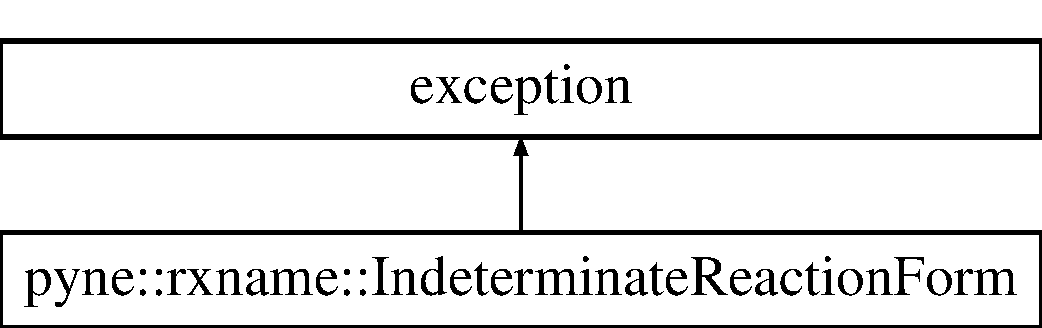
\includegraphics[height=2.000000cm]{classpyne_1_1rxname_1_1_indeterminate_reaction_form}
\end{center}
\end{figure}
\subsection*{Public Member Functions}
\begin{DoxyCompactItemize}
\item 
\hypertarget{classpyne_1_1rxname_1_1_indeterminate_reaction_form_a27a58bf85e1d384d5cf614ef72873e1b}{\hyperlink{classpyne_1_1rxname_1_1_indeterminate_reaction_form_a27a58bf85e1d384d5cf614ef72873e1b}{Indeterminate\-Reaction\-Form} ()}\label{classpyne_1_1rxname_1_1_indeterminate_reaction_form_a27a58bf85e1d384d5cf614ef72873e1b}

\begin{DoxyCompactList}\small\item\em default constructor \end{DoxyCompactList}\item 
\hypertarget{classpyne_1_1rxname_1_1_indeterminate_reaction_form_a7df25775691de519d2ccdc9a25a4e5b2}{\hyperlink{classpyne_1_1rxname_1_1_indeterminate_reaction_form_a7df25775691de519d2ccdc9a25a4e5b2}{$\sim$\-Indeterminate\-Reaction\-Form} ()  throw ()}\label{classpyne_1_1rxname_1_1_indeterminate_reaction_form_a7df25775691de519d2ccdc9a25a4e5b2}

\begin{DoxyCompactList}\small\item\em default destructor \end{DoxyCompactList}\item 
\hyperlink{classpyne_1_1rxname_1_1_indeterminate_reaction_form_ad5a88cc1f318df127516265e9f2bdc87}{Indeterminate\-Reaction\-Form} (std\-::string wasptr, std\-::string nowptr)
\item 
\hyperlink{classpyne_1_1rxname_1_1_indeterminate_reaction_form_abcbbdd0a0a16e11b20eadffc1b7af7a4}{Indeterminate\-Reaction\-Form} (std\-::string wasptr, int nowptr)
\item 
\hyperlink{classpyne_1_1rxname_1_1_indeterminate_reaction_form_ae3b4b1af4980744bfe06bdd66f2ef696}{Indeterminate\-Reaction\-Form} (int wasptr, std\-::string nowptr)
\item 
\hyperlink{classpyne_1_1rxname_1_1_indeterminate_reaction_form_a8efd3b1144d39fc11e67f4411c3b5149}{Indeterminate\-Reaction\-Form} (int wasptr, int nowptr)
\item 
\hypertarget{classpyne_1_1rxname_1_1_indeterminate_reaction_form_a7a1cf5af3d08aecd0394e7624c4918ed}{virtual const char $\ast$ \hyperlink{classpyne_1_1rxname_1_1_indeterminate_reaction_form_a7a1cf5af3d08aecd0394e7624c4918ed}{what} () const   throw ()}\label{classpyne_1_1rxname_1_1_indeterminate_reaction_form_a7a1cf5af3d08aecd0394e7624c4918ed}

\begin{DoxyCompactList}\small\item\em Returns a helpful error message containing prior and current reaction state. \end{DoxyCompactList}\end{DoxyCompactItemize}


\subsection{Detailed Description}
Custom exception for declaring a value not to be of ambiquous reaction form. 

\subsection{Constructor \& Destructor Documentation}
\hypertarget{classpyne_1_1rxname_1_1_indeterminate_reaction_form_ad5a88cc1f318df127516265e9f2bdc87}{\index{pyne\-::rxname\-::\-Indeterminate\-Reaction\-Form@{pyne\-::rxname\-::\-Indeterminate\-Reaction\-Form}!Indeterminate\-Reaction\-Form@{Indeterminate\-Reaction\-Form}}
\index{Indeterminate\-Reaction\-Form@{Indeterminate\-Reaction\-Form}!pyne::rxname::IndeterminateReactionForm@{pyne\-::rxname\-::\-Indeterminate\-Reaction\-Form}}
\subsubsection[{Indeterminate\-Reaction\-Form}]{\setlength{\rightskip}{0pt plus 5cm}pyne\-::rxname\-::\-Indeterminate\-Reaction\-Form\-::\-Indeterminate\-Reaction\-Form (
\begin{DoxyParamCaption}
\item[{std\-::string}]{wasptr, }
\item[{std\-::string}]{nowptr}
\end{DoxyParamCaption}
)\hspace{0.3cm}{\ttfamily [inline]}}}\label{classpyne_1_1rxname_1_1_indeterminate_reaction_form_ad5a88cc1f318df127516265e9f2bdc87}
Constructor using original reaction ({\itshape wasptr}) and the eventual state that Py\-N\-E calculated ({\itshape nowptr}). \hypertarget{classpyne_1_1rxname_1_1_indeterminate_reaction_form_abcbbdd0a0a16e11b20eadffc1b7af7a4}{\index{pyne\-::rxname\-::\-Indeterminate\-Reaction\-Form@{pyne\-::rxname\-::\-Indeterminate\-Reaction\-Form}!Indeterminate\-Reaction\-Form@{Indeterminate\-Reaction\-Form}}
\index{Indeterminate\-Reaction\-Form@{Indeterminate\-Reaction\-Form}!pyne::rxname::IndeterminateReactionForm@{pyne\-::rxname\-::\-Indeterminate\-Reaction\-Form}}
\subsubsection[{Indeterminate\-Reaction\-Form}]{\setlength{\rightskip}{0pt plus 5cm}pyne\-::rxname\-::\-Indeterminate\-Reaction\-Form\-::\-Indeterminate\-Reaction\-Form (
\begin{DoxyParamCaption}
\item[{std\-::string}]{wasptr, }
\item[{int}]{nowptr}
\end{DoxyParamCaption}
)\hspace{0.3cm}{\ttfamily [inline]}}}\label{classpyne_1_1rxname_1_1_indeterminate_reaction_form_abcbbdd0a0a16e11b20eadffc1b7af7a4}
Constructor using original reaction ({\itshape wasptr}) and the eventual state that Py\-N\-E calculated ({\itshape nowptr}). \hypertarget{classpyne_1_1rxname_1_1_indeterminate_reaction_form_ae3b4b1af4980744bfe06bdd66f2ef696}{\index{pyne\-::rxname\-::\-Indeterminate\-Reaction\-Form@{pyne\-::rxname\-::\-Indeterminate\-Reaction\-Form}!Indeterminate\-Reaction\-Form@{Indeterminate\-Reaction\-Form}}
\index{Indeterminate\-Reaction\-Form@{Indeterminate\-Reaction\-Form}!pyne::rxname::IndeterminateReactionForm@{pyne\-::rxname\-::\-Indeterminate\-Reaction\-Form}}
\subsubsection[{Indeterminate\-Reaction\-Form}]{\setlength{\rightskip}{0pt plus 5cm}pyne\-::rxname\-::\-Indeterminate\-Reaction\-Form\-::\-Indeterminate\-Reaction\-Form (
\begin{DoxyParamCaption}
\item[{int}]{wasptr, }
\item[{std\-::string}]{nowptr}
\end{DoxyParamCaption}
)\hspace{0.3cm}{\ttfamily [inline]}}}\label{classpyne_1_1rxname_1_1_indeterminate_reaction_form_ae3b4b1af4980744bfe06bdd66f2ef696}
Constructor using original reaction ({\itshape wasptr}) and the eventual state that Py\-N\-E calculated ({\itshape nowptr}). \hypertarget{classpyne_1_1rxname_1_1_indeterminate_reaction_form_a8efd3b1144d39fc11e67f4411c3b5149}{\index{pyne\-::rxname\-::\-Indeterminate\-Reaction\-Form@{pyne\-::rxname\-::\-Indeterminate\-Reaction\-Form}!Indeterminate\-Reaction\-Form@{Indeterminate\-Reaction\-Form}}
\index{Indeterminate\-Reaction\-Form@{Indeterminate\-Reaction\-Form}!pyne::rxname::IndeterminateReactionForm@{pyne\-::rxname\-::\-Indeterminate\-Reaction\-Form}}
\subsubsection[{Indeterminate\-Reaction\-Form}]{\setlength{\rightskip}{0pt plus 5cm}pyne\-::rxname\-::\-Indeterminate\-Reaction\-Form\-::\-Indeterminate\-Reaction\-Form (
\begin{DoxyParamCaption}
\item[{int}]{wasptr, }
\item[{int}]{nowptr}
\end{DoxyParamCaption}
)\hspace{0.3cm}{\ttfamily [inline]}}}\label{classpyne_1_1rxname_1_1_indeterminate_reaction_form_a8efd3b1144d39fc11e67f4411c3b5149}
Constructor using original reaction ({\itshape wasptr}) and the eventual state that Py\-N\-E calculated ({\itshape nowptr}). 

The documentation for this class was generated from the following file\-:\begin{DoxyCompactItemize}
\item 
/home/elliott/\-Research/pyne/src/rxname.\-h\end{DoxyCompactItemize}

\hypertarget{classspatial__solvers__3d_1_1dict__util_1_1_input_dict_error}{\section{spatial\-\_\-solvers\-\_\-3d.\-dict\-\_\-util.\-Input\-Dict\-Error Class Reference}
\label{classspatial__solvers__3d_1_1dict__util_1_1_input_dict_error}\index{spatial\-\_\-solvers\-\_\-3d.\-dict\-\_\-util.\-Input\-Dict\-Error@{spatial\-\_\-solvers\-\_\-3d.\-dict\-\_\-util.\-Input\-Dict\-Error}}
}
Inheritance diagram for spatial\-\_\-solvers\-\_\-3d.\-dict\-\_\-util.\-Input\-Dict\-Error\-:\begin{figure}[H]
\begin{center}
\leavevmode
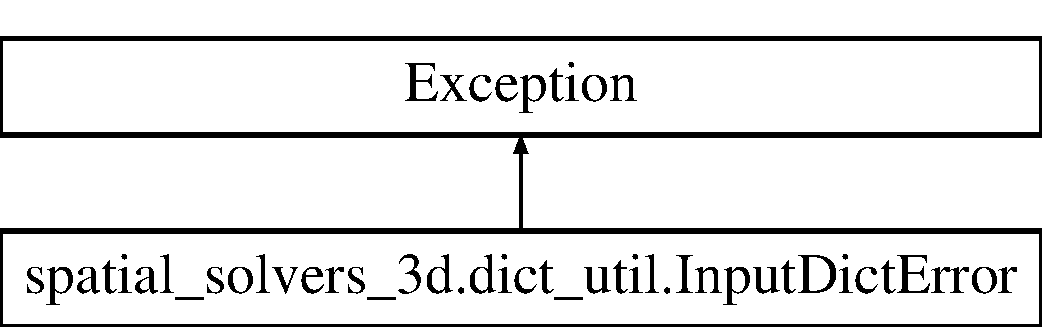
\includegraphics[height=2.000000cm]{classspatial__solvers__3d_1_1dict__util_1_1_input_dict_error}
\end{center}
\end{figure}
\subsection*{Public Member Functions}
\begin{DoxyCompactItemize}
\item 
\hypertarget{classspatial__solvers__3d_1_1dict__util_1_1_input_dict_error_a4966aa45d3b7fcb3d79a43b3d953d045}{def {\bfseries \-\_\-\-\_\-init\-\_\-\-\_\-}}\label{classspatial__solvers__3d_1_1dict__util_1_1_input_dict_error_a4966aa45d3b7fcb3d79a43b3d953d045}

\item 
\hypertarget{classspatial__solvers__3d_1_1dict__util_1_1_input_dict_error_af8d1148093139cb9f5ee4b154d3c0835}{def {\bfseries \-\_\-\-\_\-str\-\_\-\-\_\-}}\label{classspatial__solvers__3d_1_1dict__util_1_1_input_dict_error_af8d1148093139cb9f5ee4b154d3c0835}

\end{DoxyCompactItemize}
\subsection*{Public Attributes}
\begin{DoxyCompactItemize}
\item 
\hypertarget{classspatial__solvers__3d_1_1dict__util_1_1_input_dict_error_ac3622f01f73069150dcad765d8f9bd81}{{\bfseries missing}}\label{classspatial__solvers__3d_1_1dict__util_1_1_input_dict_error_ac3622f01f73069150dcad765d8f9bd81}

\end{DoxyCompactItemize}


The documentation for this class was generated from the following file\-:\begin{DoxyCompactItemize}
\item 
/home/scopatz/pyne/src/ahot/spatial\-\_\-solvers\-\_\-3d/dict\-\_\-util.\-py\end{DoxyCompactItemize}

\hypertarget{classdict__util_1_1_input_dict_error}{\section{dict\-\_\-util.\-Input\-Dict\-Error Class Reference}
\label{classdict__util_1_1_input_dict_error}\index{dict\-\_\-util.\-Input\-Dict\-Error@{dict\-\_\-util.\-Input\-Dict\-Error}}
}
Inheritance diagram for dict\-\_\-util.\-Input\-Dict\-Error\-:\begin{figure}[H]
\begin{center}
\leavevmode
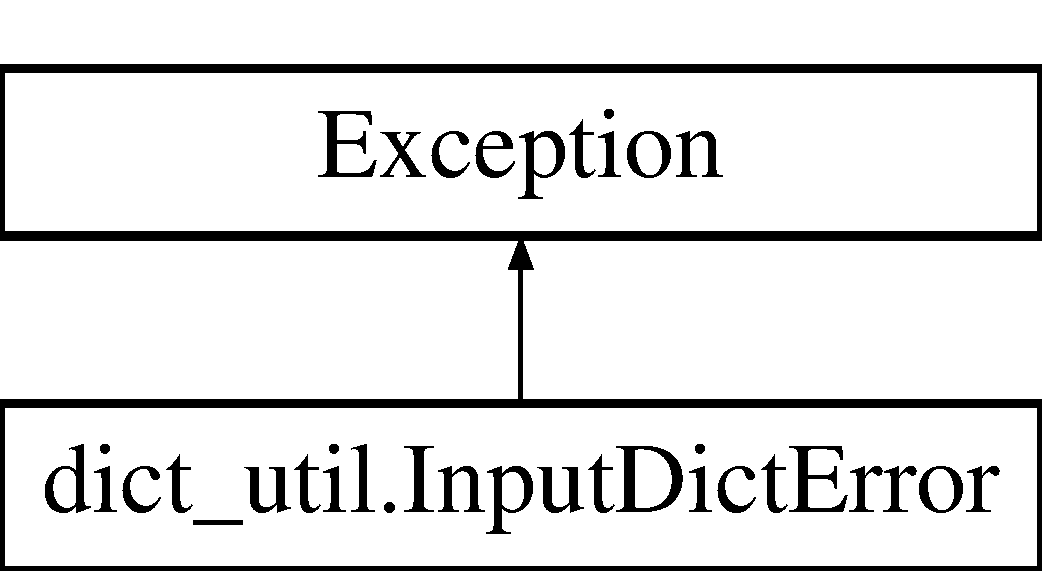
\includegraphics[height=2.000000cm]{classdict__util_1_1_input_dict_error}
\end{center}
\end{figure}
\subsection*{Public Member Functions}
\begin{DoxyCompactItemize}
\item 
\hypertarget{classdict__util_1_1_input_dict_error_a4e97e96ffaf431264fbaa99f89aa4e36}{def {\bfseries \-\_\-\-\_\-init\-\_\-\-\_\-}}\label{classdict__util_1_1_input_dict_error_a4e97e96ffaf431264fbaa99f89aa4e36}

\item 
\hypertarget{classdict__util_1_1_input_dict_error_a7227b403f5bdaba9ef675cb9cf1111e8}{def {\bfseries \-\_\-\-\_\-str\-\_\-\-\_\-}}\label{classdict__util_1_1_input_dict_error_a7227b403f5bdaba9ef675cb9cf1111e8}

\end{DoxyCompactItemize}
\subsection*{Public Attributes}
\begin{DoxyCompactItemize}
\item 
\hypertarget{classdict__util_1_1_input_dict_error_aa2ebc135b20ddafa9bae59e28bf417f1}{{\bfseries missing}}\label{classdict__util_1_1_input_dict_error_aa2ebc135b20ddafa9bae59e28bf417f1}

\end{DoxyCompactItemize}


The documentation for this class was generated from the following file\-:\begin{DoxyCompactItemize}
\item 
/home/scopatz/pyne/src/ahot/spatial\-\_\-solvers\-\_\-3d/old\-\_\-api\-\_\-solvers/dict\-\_\-util.\-py\end{DoxyCompactItemize}

\hypertarget{classpyne_1_1_invalid_simple_x_s}{\section{pyne\+:\+:Invalid\+Simple\+X\+S Class Reference}
\label{classpyne_1_1_invalid_simple_x_s}\index{pyne\+::\+Invalid\+Simple\+X\+S@{pyne\+::\+Invalid\+Simple\+X\+S}}
}


Custom exception for declaring a \hyperlink{structsimple__xs}{simple\+\_\+xs} request invalid.  




{\ttfamily \#include $<$data.\+h$>$}

Inheritance diagram for pyne\+:\+:Invalid\+Simple\+X\+S\+:\begin{figure}[H]
\begin{center}
\leavevmode
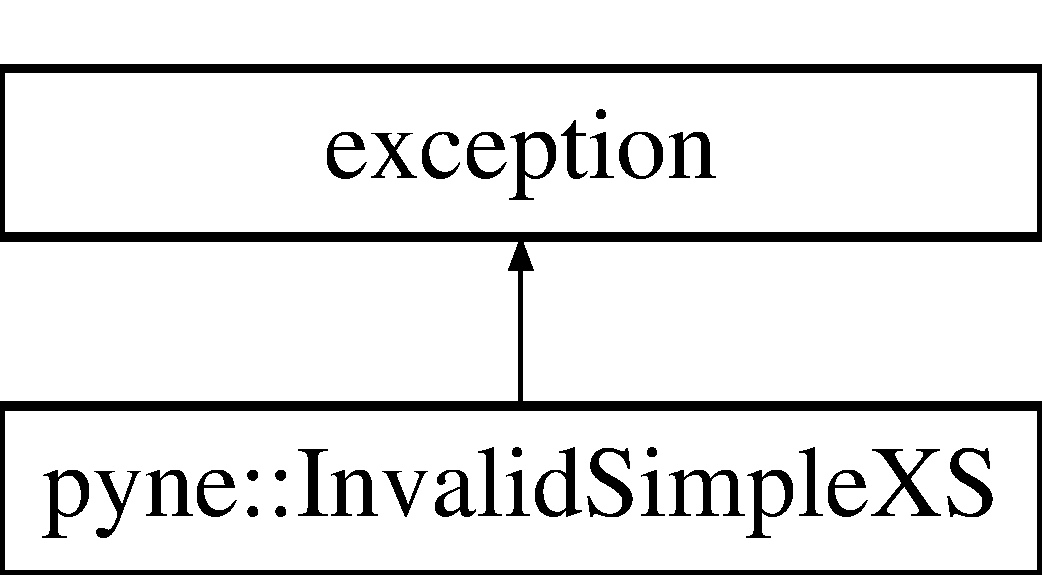
\includegraphics[height=2.000000cm]{classpyne_1_1_invalid_simple_x_s}
\end{center}
\end{figure}
\subsection*{Public Member Functions}
\begin{DoxyCompactItemize}
\item 
\hypertarget{classpyne_1_1_invalid_simple_x_s_ad3bac5f587ea476c11a622024914d074}{\hyperlink{classpyne_1_1_invalid_simple_x_s_ad3bac5f587ea476c11a622024914d074}{Invalid\+Simple\+X\+S} (std\+::string msg)}\label{classpyne_1_1_invalid_simple_x_s_ad3bac5f587ea476c11a622024914d074}

\begin{DoxyCompactList}\small\item\em Exception thrown if energy group or rxname are invalid. \end{DoxyCompactList}\item 
\hypertarget{classpyne_1_1_invalid_simple_x_s_aaafdfd9422833d680a00d7c00263b04a}{virtual const char $\ast$ \hyperlink{classpyne_1_1_invalid_simple_x_s_aaafdfd9422833d680a00d7c00263b04a}{what} () const   throw ()}\label{classpyne_1_1_invalid_simple_x_s_aaafdfd9422833d680a00d7c00263b04a}

\begin{DoxyCompactList}\small\item\em Exception returns the string passed when thrown. \end{DoxyCompactList}\end{DoxyCompactItemize}


\subsection{Detailed Description}
Custom exception for declaring a \hyperlink{structsimple__xs}{simple\+\_\+xs} request invalid. 

The documentation for this class was generated from the following file\+:\begin{DoxyCompactItemize}
\item 
/\+Users/bates26/\+Documents/pyne/src/\hyperlink{data_8h}{data.\+h}\end{DoxyCompactItemize}

\hypertarget{classinvar}{\section{invar Module Reference}
\label{classinvar}\index{invar@{invar}}
}
\subsection*{Public Attributes}
\begin{DoxyCompactItemize}
\item 
\hypertarget{classinvar_a02e121bc3c9d12618d1032db99cdec28}{character(80) {\bfseries title}}\label{classinvar_a02e121bc3c9d12618d1032db99cdec28}

\item 
\hypertarget{classinvar_a46bce44e6d673a4cc6e882ce30b1840a}{integer {\bfseries lambda}}\label{classinvar_a46bce44e6d673a4cc6e882ce30b1840a}

\item 
\hypertarget{classinvar_a481d2438b1f2df33a3cd5678af058017}{integer {\bfseries ctype}}\label{classinvar_a481d2438b1f2df33a3cd5678af058017}

\item 
\hypertarget{classinvar_aa0cf3a9d0200fd8688e2b2ec77f9956f}{integer {\bfseries meth}}\label{classinvar_aa0cf3a9d0200fd8688e2b2ec77f9956f}

\item 
\hypertarget{classinvar_a76180eb349e29c35acde311053573cde}{integer {\bfseries qdord}}\label{classinvar_a76180eb349e29c35acde311053573cde}

\item 
\hypertarget{classinvar_a9df7842f50924b762f68f20654b9b68c}{integer {\bfseries qdtyp}}\label{classinvar_a9df7842f50924b762f68f20654b9b68c}

\item 
\hypertarget{classinvar_a7926819499637fd377c0fbcc8d2ce390}{integer {\bfseries nx}}\label{classinvar_a7926819499637fd377c0fbcc8d2ce390}

\item 
\hypertarget{classinvar_a56faa93c6707a7e5b0fba189e3f7d19f}{integer {\bfseries ny}}\label{classinvar_a56faa93c6707a7e5b0fba189e3f7d19f}

\item 
\hypertarget{classinvar_a2c36e6e26f736a59f283704bd4998821}{integer {\bfseries ng}}\label{classinvar_a2c36e6e26f736a59f283704bd4998821}

\item 
\hypertarget{classinvar_ad46509578bfab6a49094b99282d36bf6}{integer {\bfseries nm}}\label{classinvar_ad46509578bfab6a49094b99282d36bf6}

\item 
\hypertarget{classinvar_a62caa28ee6cfc9246b29b2808567c112}{real $\ast$8 {\bfseries fweights}}\label{classinvar_a62caa28ee6cfc9246b29b2808567c112}

\item 
\hypertarget{classinvar_a6a89c71e56cbf68a304660d99b2d117b}{real $\ast$8, dimension(\-:), allocatable {\bfseries dx}}\label{classinvar_a6a89c71e56cbf68a304660d99b2d117b}

\item 
\hypertarget{classinvar_a204fdf570d734f509f2b291a5c118caa}{real $\ast$8, dimension(\-:), allocatable {\bfseries dy}}\label{classinvar_a204fdf570d734f509f2b291a5c118caa}

\item 
\hypertarget{classinvar_a7e75fa0b8c783ceaba90fec5c8e4c98b}{integer, dimension(\-:,\-:), \\*
allocatable {\bfseries mat}}\label{classinvar_a7e75fa0b8c783ceaba90fec5c8e4c98b}

\item 
\hypertarget{classinvar_a7852edfcc890a0c2ee575128cfded680}{integer {\bfseries lbc}}\label{classinvar_a7852edfcc890a0c2ee575128cfded680}

\item 
\hypertarget{classinvar_a861dae72d9d2fcd9ea116e650207ec18}{integer {\bfseries rbc}}\label{classinvar_a861dae72d9d2fcd9ea116e650207ec18}

\item 
\hypertarget{classinvar_a6d111f3f294d097892bd94714ac2de9b}{integer {\bfseries bbc}}\label{classinvar_a6d111f3f294d097892bd94714ac2de9b}

\item 
\hypertarget{classinvar_a0ccc322d850fbe1074cb937cde449e02}{integer {\bfseries tbc}}\label{classinvar_a0ccc322d850fbe1074cb937cde449e02}

\item 
\hypertarget{classinvar_ab909446efeb5bdca23d80d75c93731da}{real $\ast$8 {\bfseries err}}\label{classinvar_ab909446efeb5bdca23d80d75c93731da}

\item 
\hypertarget{classinvar_ab259d9aba004a4dc3064942297f86839}{real $\ast$8 {\bfseries tolr}}\label{classinvar_ab259d9aba004a4dc3064942297f86839}

\item 
\hypertarget{classinvar_aca04f7cbe921bb249c576680adbd0fd8}{integer {\bfseries itmx}}\label{classinvar_aca04f7cbe921bb249c576680adbd0fd8}

\item 
\hypertarget{classinvar_ac94f06afb54503fdcfb76aa3271f150f}{integer {\bfseries iall}}\label{classinvar_ac94f06afb54503fdcfb76aa3271f150f}

\item 
\hypertarget{classinvar_ae05f644150f4a61fb93c066519e16253}{real $\ast$8 {\bfseries tchk}}\label{classinvar_ae05f644150f4a61fb93c066519e16253}

\item 
\hypertarget{classinvar_ab341cd3ab4c4d39818e4a67f24b4f8db}{integer {\bfseries ichk}}\label{classinvar_ab341cd3ab4c4d39818e4a67f24b4f8db}

\item 
\hypertarget{classinvar_ad343382de87380b003d3cb1956f9d7f6}{integer {\bfseries apo}}\label{classinvar_ad343382de87380b003d3cb1956f9d7f6}

\item 
\hypertarget{classinvar_a61de2c440600d5d2ac76813668f8e822}{integer {\bfseries order}}\label{classinvar_a61de2c440600d5d2ac76813668f8e822}

\item 
\hypertarget{classinvar_a094a6bb02520f1985afcbd316bddfc9a}{integer {\bfseries ordsq}}\label{classinvar_a094a6bb02520f1985afcbd316bddfc9a}

\item 
\hypertarget{classinvar_aa99f29b7ae37d212b885d6a632d36baa}{real $\ast$8, dimension(\-:,\-:), \\*
allocatable {\bfseries ssum}}\label{classinvar_aa99f29b7ae37d212b885d6a632d36baa}

\item 
\hypertarget{classinvar_a42fc94342b9f9064432aca52d36a99e9}{real $\ast$8, dimension(\-:,\-:), \\*
allocatable {\bfseries ang}}\label{classinvar_a42fc94342b9f9064432aca52d36a99e9}

\item 
\hypertarget{classinvar_a3fe98ed23b01e69ed2a26e168daf3f86}{real $\ast$8, dimension(\-:), allocatable {\bfseries w}}\label{classinvar_a3fe98ed23b01e69ed2a26e168daf3f86}

\item 
\hypertarget{classinvar_a4a9f22ce179e94bf9c3fe258faae5b58}{real $\ast$8, dimension(\-:,\-:), \\*
allocatable {\bfseries sigt}}\label{classinvar_a4a9f22ce179e94bf9c3fe258faae5b58}

\item 
\hypertarget{classinvar_a9955ce132cdd8e0c1057c56696cdabbb}{real $\ast$8, dimension(\-:,\-:,\-:), \\*
allocatable {\bfseries sigs}}\label{classinvar_a9955ce132cdd8e0c1057c56696cdabbb}

\item 
\hypertarget{classinvar_a47e4465a26cc745f1145ea33a193e927}{real $\ast$8, dimension(\-:,\-:,\-:,\-:,\-:), \\*
allocatable {\bfseries s}}\label{classinvar_a47e4465a26cc745f1145ea33a193e927}

\item 
\hypertarget{classinvar_a5982621385c379b133311898f18ceea7}{real $\ast$8, dimension(\-:,\-:,\-:,\-:,\-:), \\*
allocatable {\bfseries lbsource}}\label{classinvar_a5982621385c379b133311898f18ceea7}

\item 
\hypertarget{classinvar_af86b6ba49e8aa641f79280416fafef5d}{real $\ast$8, dimension(\-:,\-:,\-:,\-:,\-:), \\*
allocatable {\bfseries rbsource}}\label{classinvar_af86b6ba49e8aa641f79280416fafef5d}

\item 
\hypertarget{classinvar_a9722eba3dc5238a62a8fdac6a95ade58}{real $\ast$8, dimension(\-:,\-:,\-:,\-:,\-:), \\*
allocatable {\bfseries bbsource}}\label{classinvar_a9722eba3dc5238a62a8fdac6a95ade58}

\item 
\hypertarget{classinvar_a16ab0726918b84dca7af0b1913c85a60}{real $\ast$8, dimension(\-:,\-:,\-:,\-:,\-:), \\*
allocatable {\bfseries tbsource}}\label{classinvar_a16ab0726918b84dca7af0b1913c85a60}

\item 
\hypertarget{classinvar_ab8459ed9952252b048bf1c9389853378}{integer {\bfseries momp}}\label{classinvar_ab8459ed9952252b048bf1c9389853378}

\item 
\hypertarget{classinvar_a6a9a8e7150242d32c89afe6f81fdb30e}{integer {\bfseries momsum}}\label{classinvar_a6a9a8e7150242d32c89afe6f81fdb30e}

\item 
\hypertarget{classinvar_a46dff67f65713ac43ebad6ac61b2b0a1}{integer {\bfseries mompt}}\label{classinvar_a46dff67f65713ac43ebad6ac61b2b0a1}

\item 
\hypertarget{classinvar_a699a57a9fdbbb5dca04f2c6803f9fa7f}{integer {\bfseries qdflx}}\label{classinvar_a699a57a9fdbbb5dca04f2c6803f9fa7f}

\item 
\hypertarget{classinvar_a007b33c5c4a704c8091cdfabf155b940}{integer {\bfseries itmflag}}\label{classinvar_a007b33c5c4a704c8091cdfabf155b940}

\item 
\hypertarget{classinvar_ad66c1deb91ee7d0e72856b25cb0bf6d4}{integer {\bfseries matrix}}\label{classinvar_ad66c1deb91ee7d0e72856b25cb0bf6d4}

\item 
\hypertarget{classinvar_adb3bfc085dfbbc76e236bf7709c98a29}{integer {\bfseries nz}}\label{classinvar_adb3bfc085dfbbc76e236bf7709c98a29}

\item 
\hypertarget{classinvar_a2e800e5321428f5226b62f5e952e9095}{real $\ast$8, dimension(\-:), allocatable {\bfseries dz}}\label{classinvar_a2e800e5321428f5226b62f5e952e9095}

\item 
\hypertarget{classinvar_a2a47bbd7a8e09bd67ee8d9df4dfc5d4c}{integer, dimension(\-:,\-:,\-:), \\*
allocatable {\bfseries mat}}\label{classinvar_a2a47bbd7a8e09bd67ee8d9df4dfc5d4c}

\item 
\hypertarget{classinvar_ac43b19b4e4bcff61f0e4f9524189c8ba}{integer {\bfseries xsbc}}\label{classinvar_ac43b19b4e4bcff61f0e4f9524189c8ba}

\item 
\hypertarget{classinvar_afdac254b51a0c1e15bcdcd5ec78ab097}{integer {\bfseries xebc}}\label{classinvar_afdac254b51a0c1e15bcdcd5ec78ab097}

\item 
\hypertarget{classinvar_a9feb27241762c9dd706e558252f092e9}{integer {\bfseries ysbc}}\label{classinvar_a9feb27241762c9dd706e558252f092e9}

\item 
\hypertarget{classinvar_a9012ac72ddd4547ce6b4b0c28701049e}{integer {\bfseries yebc}}\label{classinvar_a9012ac72ddd4547ce6b4b0c28701049e}

\item 
\hypertarget{classinvar_ab045f0221783a9b1b14a3169a13b652e}{integer {\bfseries zsbc}}\label{classinvar_ab045f0221783a9b1b14a3169a13b652e}

\item 
\hypertarget{classinvar_a6d0cbede1297cdf187502fad15cde4ea}{integer {\bfseries zebc}}\label{classinvar_a6d0cbede1297cdf187502fad15cde4ea}

\item 
\hypertarget{classinvar_ada256e2673f0bae0b39e1bed05a0691a}{integer {\bfseries ordcb}}\label{classinvar_ada256e2673f0bae0b39e1bed05a0691a}

\item 
\hypertarget{classinvar_a319dd4f77663bb45329b5f76da96cd7e}{real $\ast$8, dimension(\-:,\-:,\-:,\-:,\-:,\-:,\-:), \\*
allocatable {\bfseries s}}\label{classinvar_a319dd4f77663bb45329b5f76da96cd7e}

\item 
\hypertarget{classinvar_a1aa743a6dbe1fdb2c9a7c27939260062}{real $\ast$8, dimension(\-:,\-:,\-:,\-:,\-:,\-:), \\*
allocatable {\bfseries frbc}}\label{classinvar_a1aa743a6dbe1fdb2c9a7c27939260062}

\item 
\hypertarget{classinvar_a1d0f9c9e04a33ecb8212e2e03ca59441}{real $\ast$8, dimension(\-:,\-:,\-:,\-:,\-:,\-:), \\*
allocatable {\bfseries babc}}\label{classinvar_a1d0f9c9e04a33ecb8212e2e03ca59441}

\item 
\hypertarget{classinvar_a0881e17f3c8fa116370528daeccc3d1a}{real $\ast$8, dimension(\-:,\-:,\-:,\-:,\-:,\-:), \\*
allocatable {\bfseries lebc}}\label{classinvar_a0881e17f3c8fa116370528daeccc3d1a}

\item 
\hypertarget{classinvar_af0bda0f1e756949fb7c2f6362f568490}{real $\ast$8, dimension(\-:,\-:,\-:,\-:,\-:,\-:), \\*
allocatable {\bfseries ribc}}\label{classinvar_af0bda0f1e756949fb7c2f6362f568490}

\item 
\hypertarget{classinvar_a66e523d7c7ca8de2aa4974fd88921fd6}{real $\ast$8, dimension(\-:,\-:,\-:,\-:,\-:,\-:), \\*
allocatable {\bfseries bobc}}\label{classinvar_a66e523d7c7ca8de2aa4974fd88921fd6}

\item 
\hypertarget{classinvar_a9aef21427b8c45f2a7428aa45ead9565}{real $\ast$8, dimension(\-:,\-:,\-:,\-:,\-:,\-:), \\*
allocatable {\bfseries tobc}}\label{classinvar_a9aef21427b8c45f2a7428aa45ead9565}

\item 
\hypertarget{classinvar_a383bc7305cab31047fd3484b71783e9e}{character(30) {\bfseries solver}}\label{classinvar_a383bc7305cab31047fd3484b71783e9e}

\item 
\hypertarget{classinvar_a8ebe758a13efebeec22ef5d0ff6145c5}{character(30) {\bfseries solvertype}}\label{classinvar_a8ebe758a13efebeec22ef5d0ff6145c5}

\item 
\hypertarget{classinvar_aae7831cb3837b927d4521c09165b16d4}{integer {\bfseries dofpc}}\label{classinvar_aae7831cb3837b927d4521c09165b16d4}

\item 
\hypertarget{classinvar_a71990993acb0781c49be8cfc2d80bb91}{real $\ast$8, dimension(\-:,\-:,\-:,\-:,\-:), \\*
allocatable {\bfseries frbc}}\label{classinvar_a71990993acb0781c49be8cfc2d80bb91}

\item 
\hypertarget{classinvar_a7a5af3f927be39433c87341ca9c01e8c}{real $\ast$8, dimension(\-:,\-:,\-:,\-:,\-:), \\*
allocatable {\bfseries babc}}\label{classinvar_a7a5af3f927be39433c87341ca9c01e8c}

\item 
\hypertarget{classinvar_a128ebdaef308bb3f73788bc98fb8ef74}{real $\ast$8, dimension(\-:,\-:,\-:,\-:,\-:), \\*
allocatable {\bfseries lebc}}\label{classinvar_a128ebdaef308bb3f73788bc98fb8ef74}

\item 
\hypertarget{classinvar_ae6974a09ecc9cb418528ece1f5cb4955}{real $\ast$8, dimension(\-:,\-:,\-:,\-:,\-:), \\*
allocatable {\bfseries ribc}}\label{classinvar_ae6974a09ecc9cb418528ece1f5cb4955}

\item 
\hypertarget{classinvar_aff431f9b7accdbcb2fb50faa07f9c3bf}{real $\ast$8, dimension(\-:,\-:,\-:,\-:,\-:), \\*
allocatable {\bfseries bobc}}\label{classinvar_aff431f9b7accdbcb2fb50faa07f9c3bf}

\item 
\hypertarget{classinvar_aa602d92324bf37bc88b28e775e679a72}{real $\ast$8, dimension(\-:,\-:,\-:,\-:,\-:), \\*
allocatable {\bfseries tobc}}\label{classinvar_aa602d92324bf37bc88b28e775e679a72}

\item 
\hypertarget{classinvar_aed524b8b860286a546c5ad47da27942a}{real $\ast$8, dimension(\-:,\-:,\-:,\-:,\-:,\-:), \\*
allocatable {\bfseries tfrbc}}\label{classinvar_aed524b8b860286a546c5ad47da27942a}

\item 
\hypertarget{classinvar_acb84bd013b528d78ad5df94841e50594}{real $\ast$8, dimension(\-:,\-:,\-:,\-:,\-:,\-:), \\*
allocatable {\bfseries tbabc}}\label{classinvar_acb84bd013b528d78ad5df94841e50594}

\item 
\hypertarget{classinvar_a32d8b5b0175a00ff35c34b207d47106d}{real $\ast$8, dimension(\-:,\-:,\-:,\-:,\-:,\-:), \\*
allocatable {\bfseries tlebc}}\label{classinvar_a32d8b5b0175a00ff35c34b207d47106d}

\item 
\hypertarget{classinvar_abd1adf238e31c46a52785d65dfbffeea}{real $\ast$8, dimension(\-:,\-:,\-:,\-:,\-:,\-:), \\*
allocatable {\bfseries tribc}}\label{classinvar_abd1adf238e31c46a52785d65dfbffeea}

\item 
\hypertarget{classinvar_a3657d6ac0059ed40591fb6d217b57a75}{real $\ast$8, dimension(\-:,\-:,\-:,\-:,\-:,\-:), \\*
allocatable {\bfseries tbobc}}\label{classinvar_a3657d6ac0059ed40591fb6d217b57a75}

\item 
\hypertarget{classinvar_ae7e2353187feafbf60577a1e855276a6}{real $\ast$8, dimension(\-:,\-:,\-:,\-:,\-:,\-:), \\*
allocatable {\bfseries ttobc}}\label{classinvar_ae7e2353187feafbf60577a1e855276a6}

\item 
\hypertarget{classinvar_a1cc177af4829d262d85a0a2451b92df7}{integer {\bfseries orpc}}\label{classinvar_a1cc177af4829d262d85a0a2451b92df7}

\item 
\hypertarget{classinvar_a2a9334ce62d1b88d5eef78527da95010}{real $\ast$8, dimension(\-:,\-:,\-:,\-:), \\*
allocatable {\bfseries s}}\label{classinvar_a2a9334ce62d1b88d5eef78527da95010}

\item 
\hypertarget{classinvar_ace772218e498ad1c568fdf7b11233abb}{real $\ast$8, dimension(\-:,\-:,\-:,\-:), \\*
allocatable {\bfseries frbc}}\label{classinvar_ace772218e498ad1c568fdf7b11233abb}

\item 
\hypertarget{classinvar_a918a37d715d375e12c4a082c3c3dd12c}{real $\ast$8, dimension(\-:,\-:,\-:,\-:), \\*
allocatable {\bfseries babc}}\label{classinvar_a918a37d715d375e12c4a082c3c3dd12c}

\item 
\hypertarget{classinvar_a44f9f17e08b9b3c233d120dc27ba407e}{real $\ast$8, dimension(\-:,\-:,\-:,\-:), \\*
allocatable {\bfseries lebc}}\label{classinvar_a44f9f17e08b9b3c233d120dc27ba407e}

\item 
\hypertarget{classinvar_a8e0f72dd980f7ef5159bfbe9d4cce0bb}{real $\ast$8, dimension(\-:,\-:,\-:,\-:), \\*
allocatable {\bfseries ribc}}\label{classinvar_a8e0f72dd980f7ef5159bfbe9d4cce0bb}

\item 
\hypertarget{classinvar_ac88ff3a97a0eccbee288774e812dce01}{real $\ast$8, dimension(\-:,\-:,\-:,\-:), \\*
allocatable {\bfseries bobc}}\label{classinvar_ac88ff3a97a0eccbee288774e812dce01}

\item 
\hypertarget{classinvar_ae61fcd8c1e76af2c5a1700a1beea040e}{real $\ast$8, dimension(\-:,\-:,\-:,\-:), \\*
allocatable {\bfseries tobc}}\label{classinvar_ae61fcd8c1e76af2c5a1700a1beea040e}

\end{DoxyCompactItemize}


The documentation for this module was generated from the following files\-:\begin{DoxyCompactItemize}
\item 
/home/elliott/\-Research/pyne/src/ahot/spatial\-\_\-solvers\-\_\-2d/src/invar.\-f90\item 
/home/elliott/\-Research/pyne/src/ahot/spatial\-\_\-solvers\-\_\-3d/\-A\-H\-O\-T\-N/src\-\_\-\-A\-H\-O\-T\-N\-\_\-\-N\-E\-F\-D\-\_\-gesv/invar.\-f90\item 
/home/elliott/\-Research/pyne/src/ahot/spatial\-\_\-solvers\-\_\-3d/\-A\-H\-O\-T\-N/src\-\_\-\-L\-L/invar.\-f90\item 
/home/elliott/\-Research/pyne/src/ahot/spatial\-\_\-solvers\-\_\-3d/\-A\-H\-O\-T\-N/src\-\_\-\-L\-L/old/invar.\-f90\item 
/home/elliott/\-Research/pyne/src/ahot/spatial\-\_\-solvers\-\_\-3d/\-A\-H\-O\-T\-N/src\-\_\-\-L\-N/invar.\-f90\item 
/home/elliott/\-Research/pyne/src/ahot/spatial\-\_\-solvers\-\_\-3d/\-D\-G\-F\-E\-M/src\-\_\-dgfem\-\_\-complete\-\_\-solver\-\_\-dense/invar.\-f90\item 
/home/elliott/\-Research/pyne/src/ahot/spatial\-\_\-solvers\-\_\-3d/\-D\-G\-F\-E\-M/src\-\_\-dgfem\-\_\-lagrange\-\_\-solver\-\_\-dense/invar.\-f90\item 
/home/elliott/\-Research/pyne/src/ahot/spatial\-\_\-solvers\-\_\-3d/\-D\-G\-F\-E\-M/src\-\_\-\-L\-D\-\_\-solver/invar.\-f90\item 
/home/elliott/\-Research/pyne/src/ahot/spatial\-\_\-solvers\-\_\-3d/\-D\-G\-F\-E\-M\-\_\-source/invar.\-f90\item 
/home/elliott/\-Research/pyne/src/ahot/spatial\-\_\-solvers\-\_\-3d/\-S\-C\-T-\/\-Step/src\-\_\-ahotn-\/step-\/sct/invar.\-f90\item 
/home/elliott/\-Research/pyne/src/ahot/spatial\-\_\-solvers\-\_\-3d/source/invar.\-f90\end{DoxyCompactItemize}

\hypertarget{classkernel__module}{\section{kernel\-\_\-module Module Reference}
\label{classkernel__module}\index{kernel\-\_\-module@{kernel\-\_\-module}}
}
\subsection*{Public Member Functions}
\begin{DoxyCompactItemize}
\item 
\hypertarget{classkernel__module_ac5350d99b77155ff299f25b6d70cea2d}{subroutine {\bfseries read\-\_\-sp\-\_\-wts} (order)}\label{classkernel__module_ac5350d99b77155ff299f25b6d70cea2d}

\item 
\hypertarget{classkernel__module_a6c7125e68f81cb0e7cd9f3e48abc126e}{real $\ast$8 function {\bfseries spwt} (e)}\label{classkernel__module_a6c7125e68f81cb0e7cd9f3e48abc126e}

\item 
\hypertarget{classkernel__module_a23d3af9299716bd83f7c2cd31d59bd4f}{subroutine {\bfseries ahotn0\-\_\-kernel} (x, y, z, mu, eta, xi, sig, inflow\-\_\-x, inflow\-\_\-y, inflow\-\_\-z, psia)}\label{classkernel__module_a23d3af9299716bd83f7c2cd31d59bd4f}

\item 
\hypertarget{classkernel__module_af428ae06d5e559edbf278d33f3628296}{subroutine {\bfseries step\-\_\-kernel} (sigt, mu, eta, xi, sc\-\_\-pol, nfaces\-\_\-x, nfaces\-\_\-y, nfaces\-\_\-z, fx, fy, fz, b)}\label{classkernel__module_af428ae06d5e559edbf278d33f3628296}

\item 
\hypertarget{classkernel__module_aa7cb328967dc7b6b33a0c922daed7cb7}{subroutine {\bfseries read\-\_\-sp\-\_\-wts\-\_\-ahotn\-\_\-l}}\label{classkernel__module_aa7cb328967dc7b6b33a0c922daed7cb7}

\item 
\hypertarget{classkernel__module_a0e94ea76b266be88663f608c0646f6d1}{real $\ast$8 function {\bfseries spwt0} (e)}\label{classkernel__module_a0e94ea76b266be88663f608c0646f6d1}

\item 
\hypertarget{classkernel__module_aa29c22ba87ecbc4ba8ab0d04c54783e0}{real $\ast$8 function {\bfseries spwt1} (e)}\label{classkernel__module_aa29c22ba87ecbc4ba8ab0d04c54783e0}

\item 
\hypertarget{classkernel__module_aa7132726727d08e3e2637052f59abdad}{real(kind=8) function {\bfseries wt0} (t)}\label{classkernel__module_aa7132726727d08e3e2637052f59abdad}

\item 
\hypertarget{classkernel__module_a2167a318581a58f1b295119931ddd408}{real(kind=8) function {\bfseries wt1} (t)}\label{classkernel__module_a2167a318581a58f1b295119931ddd408}

\item 
\hypertarget{classkernel__module_a4074268fc2e0b2ba21b5ad39eec86ab3}{subroutine {\bfseries read\-\_\-sp\-\_\-wts\-\_\-ahotn\-\_\-nefd} (order)}\label{classkernel__module_a4074268fc2e0b2ba21b5ad39eec86ab3}

\item 
\hypertarget{classkernel__module_a6c7125e68f81cb0e7cd9f3e48abc126e}{real $\ast$8 function {\bfseries spwt} (e)}\label{classkernel__module_a6c7125e68f81cb0e7cd9f3e48abc126e}

\item 
\hypertarget{classkernel__module_a3d3eccec75c0ba28bb09ab8ca22818bc}{subroutine {\bfseries ahotn\-\_\-ln\-\_\-kernel} (x, y, z, mu, eta, xi, sgm, sge, sgx, sig, c, inflow\-\_\-x, inflow\-\_\-y, inflow\-\_\-z, b)}\label{classkernel__module_a3d3eccec75c0ba28bb09ab8ca22818bc}

\item 
\hypertarget{classkernel__module_a98095dff722fb7046e5b08932b02149d}{subroutine {\bfseries ahotn\-\_\-ll\-\_\-kernel} (x, y, z, mu, eta, xi, sgm, sge, sgx, sig, c, inflow\-\_\-x, inflow\-\_\-y, inflow\-\_\-z, b)}\label{classkernel__module_a98095dff722fb7046e5b08932b02149d}

\item 
\hypertarget{classkernel__module_aa6341d47b5386becb826bdbb16be5e89}{subroutine {\bfseries ahotn\-\_\-nefd\-\_\-kernel} (x, y, z, mu, eta, xi, sgm, sge, sgx, sig, c, inflow\-\_\-x, inflow\-\_\-y, inflow\-\_\-z, b, lambda, ordcb)}\label{classkernel__module_aa6341d47b5386becb826bdbb16be5e89}

\end{DoxyCompactItemize}
\subsection*{Public Attributes}
\begin{DoxyCompactItemize}
\item 
\hypertarget{classkernel__module_ad2a8647b9f46d5c36966764ba8084d64}{real(kind=8), dimension(4, 0\-:1000) {\bfseries sp\-\_\-wts}}\label{classkernel__module_ad2a8647b9f46d5c36966764ba8084d64}

\item 
\hypertarget{classkernel__module_a56176b696afbc435b81f6c7ebd75f287}{real $\ast$8, dimension(4, 0\-:1000) {\bfseries sp\-\_\-wt0}}\label{classkernel__module_a56176b696afbc435b81f6c7ebd75f287}

\item 
\hypertarget{classkernel__module_a9c85ae778290368b8125e6548542c20c}{real $\ast$8, dimension(4, 0\-:1000) {\bfseries sp\-\_\-wt1}}\label{classkernel__module_a9c85ae778290368b8125e6548542c20c}

\end{DoxyCompactItemize}


The documentation for this module was generated from the following files\-:\begin{DoxyCompactItemize}
\item 
/home/scopatz/pyne/src/ahot/spatial\-\_\-solvers\-\_\-3d/\-S\-C\-T-\/\-Step/src\-\_\-ahotn-\/step-\/sct/kernel\-\_\-module.\-f90\item 
/home/scopatz/pyne/src/ahot/spatial\-\_\-solvers\-\_\-3d/source/ahotn\-\_\-kernel\-\_\-module.\-f90\end{DoxyCompactItemize}

\hypertarget{classld__module}{\section{ld\+\_\+module Module Reference}
\label{classld__module}\index{ld\+\_\+module@{ld\+\_\+module}}
}
\subsection*{Public Member Functions}
\begin{DoxyCompactItemize}
\item 
\hypertarget{classld__module_a7b1e55ba9bbc02396f0a489ad630cfde}{subroutine {\bfseries ld\+\_\+kernel} (del, sigt, omega, face\+\_\+psi, vecx)}\label{classld__module_a7b1e55ba9bbc02396f0a489ad630cfde}

\end{DoxyCompactItemize}


The documentation for this module was generated from the following file\+:\begin{DoxyCompactItemize}
\item 
/\+Users/bates26/\+Documents/pyne/src/ahot/spatial\+\_\+solvers\+\_\+3d/\+D\+G\+F\+E\+M/src\+\_\+\+L\+D\+\_\+solver/ld.\+f90\end{DoxyCompactItemize}

\hypertarget{structpyne_1_1level__data}{\section{pyne\-:\-:level\-\_\-data Struct Reference}
\label{structpyne_1_1level__data}\index{pyne\-::level\-\_\-data@{pyne\-::level\-\_\-data}}
}


a struct matching the '/decay/level\-\_\-list' table in nuc\-\_\-data.\-h5.  




{\ttfamily \#include $<$data.\-h$>$}

\subsection*{Public Attributes}
\begin{DoxyCompactItemize}
\item 
\hypertarget{structpyne_1_1level__data_aefac68a7a5aaedafd0b01f459e75adc8}{int \hyperlink{structpyne_1_1level__data_aefac68a7a5aaedafd0b01f459e75adc8}{nuc\-\_\-id}}\label{structpyne_1_1level__data_aefac68a7a5aaedafd0b01f459e75adc8}

\begin{DoxyCompactList}\small\item\em state id of nuclide \end{DoxyCompactList}\item 
\hypertarget{structpyne_1_1level__data_a52a8e7987f8f2a01fe7142bac5ab6adc}{unsigned int \hyperlink{structpyne_1_1level__data_a52a8e7987f8f2a01fe7142bac5ab6adc}{rx\-\_\-id}}\label{structpyne_1_1level__data_a52a8e7987f8f2a01fe7142bac5ab6adc}

\begin{DoxyCompactList}\small\item\em rx id of reaction, 0 for basic level data \end{DoxyCompactList}\item 
\hypertarget{structpyne_1_1level__data_a044daae5c914e096c423b95da1586dc0}{double \hyperlink{structpyne_1_1level__data_a044daae5c914e096c423b95da1586dc0}{half\-\_\-life}}\label{structpyne_1_1level__data_a044daae5c914e096c423b95da1586dc0}

\begin{DoxyCompactList}\small\item\em half life \mbox{[}seconds\mbox{]} \end{DoxyCompactList}\item 
\hypertarget{structpyne_1_1level__data_af029059b5f79cfa2ad22e6f9fcb04ac9}{double \hyperlink{structpyne_1_1level__data_af029059b5f79cfa2ad22e6f9fcb04ac9}{level}}\label{structpyne_1_1level__data_af029059b5f79cfa2ad22e6f9fcb04ac9}

\begin{DoxyCompactList}\small\item\em level energy \mbox{[}ke\-V\mbox{]} \end{DoxyCompactList}\item 
\hypertarget{structpyne_1_1level__data_a5ce97c540e0ce558156e5a43510a4633}{double \hyperlink{structpyne_1_1level__data_a5ce97c540e0ce558156e5a43510a4633}{branch\-\_\-ratio}}\label{structpyne_1_1level__data_a5ce97c540e0ce558156e5a43510a4633}

\begin{DoxyCompactList}\small\item\em branch ratio \mbox{[}fraction\mbox{]} \end{DoxyCompactList}\item 
\hypertarget{structpyne_1_1level__data_a7a71068eed39597f007cc6624727e954}{int \hyperlink{structpyne_1_1level__data_a7a71068eed39597f007cc6624727e954}{metastable}}\label{structpyne_1_1level__data_a7a71068eed39597f007cc6624727e954}

\begin{DoxyCompactList}\small\item\em metastable level \mbox{[}int\mbox{]} \end{DoxyCompactList}\item 
\hypertarget{structpyne_1_1level__data_acabc31aa71741dbc2ea5485ca51da0d6}{char \hyperlink{structpyne_1_1level__data_acabc31aa71741dbc2ea5485ca51da0d6}{special}}\label{structpyne_1_1level__data_acabc31aa71741dbc2ea5485ca51da0d6}

\begin{DoxyCompactList}\small\item\em special high-\/spin state \mbox{[}character\mbox{]} \end{DoxyCompactList}\end{DoxyCompactItemize}


\subsection{Detailed Description}
a struct matching the '/decay/level\-\_\-list' table in nuc\-\_\-data.\-h5. 

The documentation for this struct was generated from the following file\-:\begin{DoxyCompactItemize}
\item 
/home/elliott/\-Research/pyne/src/\hyperlink{data_8h}{data.\-h}\end{DoxyCompactItemize}

\hypertarget{classll__kernel__module}{\section{ll\+\_\+kernel\+\_\+module Module Reference}
\label{classll__kernel__module}\index{ll\+\_\+kernel\+\_\+module@{ll\+\_\+kernel\+\_\+module}}
}
\subsection*{Public Member Functions}
\begin{DoxyCompactItemize}
\item 
\hypertarget{classll__kernel__module_ae64b1d2d995c0e8c9d1014c83252100a}{subroutine {\bfseries read\+\_\+sp\+\_\+wts}}\label{classll__kernel__module_ae64b1d2d995c0e8c9d1014c83252100a}

\item 
\hypertarget{classll__kernel__module_abd3403d056c55f29237c37458c205516}{real $\ast$8 function {\bfseries spwt0} (e)}\label{classll__kernel__module_abd3403d056c55f29237c37458c205516}

\item 
\hypertarget{classll__kernel__module_a79e47a1da308cac21d2f614706b336a5}{real $\ast$8 function {\bfseries spwt1} (e)}\label{classll__kernel__module_a79e47a1da308cac21d2f614706b336a5}

\item 
\hypertarget{classll__kernel__module_a0f8329a7949f76c5316682e710a76f11}{real(kind=8) function {\bfseries wt0} (t)}\label{classll__kernel__module_a0f8329a7949f76c5316682e710a76f11}

\item 
\hypertarget{classll__kernel__module_a8e6ae1b763dd657b55e2eba5bd311e2f}{real(kind=8) function {\bfseries wt1} (t)}\label{classll__kernel__module_a8e6ae1b763dd657b55e2eba5bd311e2f}

\item 
\hypertarget{classll__kernel__module_a27d3794c74e14ccbb0297fd8ebdccdd3}{subroutine {\bfseries ll\+\_\+kernel} (x, y, z, mu, eta, xi, sgm, sge, sgx, sig, c, inflow\+\_\+x, inflow\+\_\+y, inflow\+\_\+z, b)}\label{classll__kernel__module_a27d3794c74e14ccbb0297fd8ebdccdd3}

\end{DoxyCompactItemize}
\subsection*{Public Attributes}
\begin{DoxyCompactItemize}
\item 
\hypertarget{classll__kernel__module_a4f8600d6061bd3d372282cac9efbab25}{real $\ast$8, dimension(4, 0\+:1000) {\bfseries sp\+\_\+wt0}}\label{classll__kernel__module_a4f8600d6061bd3d372282cac9efbab25}

\item 
\hypertarget{classll__kernel__module_ae9ebcee33ee11a014a911c8f1552c216}{real $\ast$8, dimension(4, 0\+:1000) {\bfseries sp\+\_\+wt1}}\label{classll__kernel__module_ae9ebcee33ee11a014a911c8f1552c216}

\end{DoxyCompactItemize}


The documentation for this module was generated from the following file\+:\begin{DoxyCompactItemize}
\item 
/\+Users/bates26/\+Documents/pyne/src/ahot/spatial\+\_\+solvers\+\_\+3d/\+A\+H\+O\+T\+N/src\+\_\+\+L\+L/ll\+\_\+module.\+f90\end{DoxyCompactItemize}

\hypertarget{classln__kernel__module}{\section{ln\+\_\+kernel\+\_\+module Module Reference}
\label{classln__kernel__module}\index{ln\+\_\+kernel\+\_\+module@{ln\+\_\+kernel\+\_\+module}}
}
\subsection*{Public Member Functions}
\begin{DoxyCompactItemize}
\item 
\hypertarget{classln__kernel__module_aad8f2e59c335886b3a8a50e3f132eaa5}{subroutine {\bfseries read\+\_\+sp\+\_\+wts}}\label{classln__kernel__module_aad8f2e59c335886b3a8a50e3f132eaa5}

\item 
\hypertarget{classln__kernel__module_a2714ae332964aba16f4bf2490d4ad586}{real $\ast$8 function {\bfseries spwt0} (e)}\label{classln__kernel__module_a2714ae332964aba16f4bf2490d4ad586}

\item 
\hypertarget{classln__kernel__module_a96ab2ee2973c0667493bf3d5fd00ba04}{real $\ast$8 function {\bfseries spwt1} (e)}\label{classln__kernel__module_a96ab2ee2973c0667493bf3d5fd00ba04}

\item 
\hypertarget{classln__kernel__module_a9ab6aa3cccdaf9b53a929dd30a31961b}{real(kind=8) function {\bfseries wt0} (t)}\label{classln__kernel__module_a9ab6aa3cccdaf9b53a929dd30a31961b}

\item 
\hypertarget{classln__kernel__module_a61433a9c616f7e015071386c1ce8ea4e}{real(kind=8) function {\bfseries wt1} (t)}\label{classln__kernel__module_a61433a9c616f7e015071386c1ce8ea4e}

\item 
\hypertarget{classln__kernel__module_a656058bc673334c98c866f725c8f6c30}{subroutine {\bfseries ln\+\_\+kernel} (x, y, z, mu, eta, xi, sgm, sge, sgx, sig, c, inflow\+\_\+x, inflow\+\_\+y, inflow\+\_\+z, b)}\label{classln__kernel__module_a656058bc673334c98c866f725c8f6c30}

\end{DoxyCompactItemize}
\subsection*{Public Attributes}
\begin{DoxyCompactItemize}
\item 
\hypertarget{classln__kernel__module_acb86edae3ad6ba5f5d76b8480cc1a0c3}{real $\ast$8, dimension(4, 0\+:1000) {\bfseries sp\+\_\+wt0}}\label{classln__kernel__module_acb86edae3ad6ba5f5d76b8480cc1a0c3}

\item 
\hypertarget{classln__kernel__module_a0b4b87e5c568b8a78eaababf7fc2ffba}{real $\ast$8, dimension(4, 0\+:1000) {\bfseries sp\+\_\+wt1}}\label{classln__kernel__module_a0b4b87e5c568b8a78eaababf7fc2ffba}

\end{DoxyCompactItemize}


The documentation for this module was generated from the following file\+:\begin{DoxyCompactItemize}
\item 
/\+Users/bates26/\+Documents/pyne/src/ahot/spatial\+\_\+solvers\+\_\+3d/\+A\+H\+O\+T\+N/src\+\_\+\+L\+N/lin\+\_\+nodal\+\_\+module.\+f90\end{DoxyCompactItemize}

\hypertarget{classpyne_1_1_material}{\section{pyne\-:\-:Material Class Reference}
\label{classpyne_1_1_material}\index{pyne\-::\-Material@{pyne\-::\-Material}}
}


\hyperlink{classpyne_1_1_material}{Material} composed of nuclides.  




{\ttfamily \#include $<$material.\-h$>$}

\subsection*{Public Member Functions}
\begin{DoxyCompactItemize}
\item 
\hyperlink{classpyne_1_1_material_af9ff0462388696834a886b2e284ccd4e}{Material} ()
\item 
\hyperlink{classpyne_1_1_material_a0704a8fc8a7599cb271c349240f37538}{Material} (\hyperlink{namespacepyne_a86738cecccf4ce3f4ecc2ff6f45ce1a2}{comp\-\_\-map} cm, double m=-\/1.\-0, double d=-\/1.\-0, double apm=-\/1.\-0, Json\-::\-Value attributes=Json\-::\-Value(\hyperlink{namespace_json_a7d654b75c16a57007925868e38212b4eae8386dcfc36d1ae897745f7b4f77a1f6}{Json\-::object\-Value}))
\item 
\hyperlink{classpyne_1_1_material_a9119502ada318009bebedfb429d534d6}{Material} (char $\ast$filename, double m=-\/1.\-0, double d=-\/1.\-0, double apm=-\/1.\-0, Json\-::\-Value attributes=Json\-::\-Value(\hyperlink{namespace_json_a7d654b75c16a57007925868e38212b4eae8386dcfc36d1ae897745f7b4f77a1f6}{Json\-::object\-Value}))
\item 
\hyperlink{classpyne_1_1_material_ad8f2148f252f71de8f699d58003ca050}{Material} (std\-::string filename, double m=-\/1.\-0, double d=-\/1.\-0, double apm=-\/1.\-0, Json\-::\-Value attributes=Json\-::\-Value(\hyperlink{namespace_json_a7d654b75c16a57007925868e38212b4eae8386dcfc36d1ae897745f7b4f77a1f6}{Json\-::object\-Value}))
\item 
\hypertarget{classpyne_1_1_material_ae75f45397f12797356940e62d13fcc6f}{\hyperlink{classpyne_1_1_material_ae75f45397f12797356940e62d13fcc6f}{$\sim$\-Material} ()}\label{classpyne_1_1_material_ae75f45397f12797356940e62d13fcc6f}

\begin{DoxyCompactList}\small\item\em default destructor \end{DoxyCompactList}\item 
\hypertarget{classpyne_1_1_material_a1d4f70382d3c4ad060977de853d23d6c}{void \hyperlink{classpyne_1_1_material_a1d4f70382d3c4ad060977de853d23d6c}{norm\-\_\-comp} ()}\label{classpyne_1_1_material_a1d4f70382d3c4ad060977de853d23d6c}

\begin{DoxyCompactList}\small\item\em Normalizes the mass values in the composition. \end{DoxyCompactList}\item 
void \hyperlink{classpyne_1_1_material_a53c124ac70017813b4893a2f7fe3db6a}{\-\_\-load\-\_\-comp\-\_\-protocol0} (hid\-\_\-t db, std\-::string datapath, int row)
\item 
void \hyperlink{classpyne_1_1_material_a8b46ba10cebb01cd36a5379e363267b1}{\-\_\-load\-\_\-comp\-\_\-protocol1} (hid\-\_\-t db, std\-::string datapath, int row)
\item 
void \hyperlink{classpyne_1_1_material_a8f06385fde86492d1291b35fa982c753}{from\-\_\-hdf5} (char $\ast$filename, char $\ast$datapath, int row=-\/1, int protocol=1)
\item 
void \hyperlink{classpyne_1_1_material_ac6bc51ed739f2f735467baf14716d825}{from\-\_\-hdf5} (std\-::string filename, std\-::string datapath=\char`\"{}/material\char`\"{}, int row=-\/1, int protocol=1)
\item 
void \hyperlink{classpyne_1_1_material_adf226509fcdbf44476019fde3ff2f6ee}{write\-\_\-hdf5} (char $\ast$filename, char $\ast$datapath, char $\ast$nucpath, float row=-\/0.\-0, int chunksize=100)
\item 
void \hyperlink{classpyne_1_1_material_a9c5e1c52faafe841ff2227d08ba7aaf7}{write\-\_\-hdf5} (std\-::string filename, std\-::string datapath=\char`\"{}/material\char`\"{}, std\-::string nucpath=\char`\"{}/nucid\char`\"{}, float row=-\/0.\-0, int chunksize=100)
\item 
\hypertarget{classpyne_1_1_material_ac30ed9f082dc76a0c535eb9237a6c528}{std\-::string \hyperlink{classpyne_1_1_material_ac30ed9f082dc76a0c535eb9237a6c528}{mcnp} (std\-::string frac\-\_\-type=\char`\"{}mass\char`\"{})}\label{classpyne_1_1_material_ac30ed9f082dc76a0c535eb9237a6c528}

\begin{DoxyCompactList}\small\item\em Return an mcnp input deck record as a string. \end{DoxyCompactList}\item 
std\-::string \hyperlink{classpyne_1_1_material_a6bcd10072abbf3e9a8bcaa466f8be569}{fluka} (int id, std\-::string frac\-\_\-type=\char`\"{}mass\char`\"{})
\item 
bool \hyperlink{classpyne_1_1_material_a97461e1c6a87d91ed1293adbe43cb29e}{not\-\_\-fluka\-\_\-builtin} (std\-::string fluka\-\_\-name)
\begin{DoxyCompactList}\small\item\em Convenience function to tell whether a given name needs a material card. \end{DoxyCompactList}\item 
std\-::string \hyperlink{classpyne_1_1_material_af3f7e0865a7a8019e02c2fb3c408c2f3}{fluka\-\_\-material\-\_\-str} (int id)
\begin{DoxyCompactList}\small\item\em High level call to get details and call material\-\_\-component(..) \end{DoxyCompactList}\item 
std\-::string \hyperlink{classpyne_1_1_material_a3b7bc2f7ca3f2c05860004ea27ebcadb}{fluka\-\_\-material\-\_\-component} (int fid, int nucid, std\-::string fluka\-\_\-name)
\begin{DoxyCompactList}\small\item\em Intermediate level call to prepare final info and call material\-\_\-line(..) \end{DoxyCompactList}\item 
std\-::string \hyperlink{classpyne_1_1_material_a269b13dac00eb3ba0ff31feb5bd3b0ca}{fluka\-\_\-material\-\_\-line} (int znum, double \hyperlink{namespacepyne_aaab79c2417fc60c1a248dd702403befb}{atomic\-\_\-mass}, int fid, std\-::string fluka\-\_\-name)
\begin{DoxyCompactList}\small\item\em Format information into a F\-L\-U\-K\-A material card. \end{DoxyCompactList}\item 
std\-::string \hyperlink{classpyne_1_1_material_ab5fb8d5171b210a7c151d6bb1e180693}{fluka\-\_\-format\-\_\-field} (float field)
\begin{DoxyCompactList}\small\item\em Convenience function to format a single fluka field. \end{DoxyCompactList}\item 
std\-::string \hyperlink{classpyne_1_1_material_a3dd223f881e39c1c6014c2b79c9ee39b}{fluka\-\_\-compound\-\_\-str} (int id, std\-::string frac\-\_\-type=\char`\"{}mass\char`\"{})
\item 
\hypertarget{classpyne_1_1_material_a28d8f7a7b06110a8be097c8e7b1fc59a}{void \hyperlink{classpyne_1_1_material_a28d8f7a7b06110a8be097c8e7b1fc59a}{from\-\_\-text} (char $\ast$filename)}\label{classpyne_1_1_material_a28d8f7a7b06110a8be097c8e7b1fc59a}

\begin{DoxyCompactList}\small\item\em Reads data from a plaintext file at {\itshape filename} into this \hyperlink{classpyne_1_1_material}{Material} instance. \end{DoxyCompactList}\item 
\hypertarget{classpyne_1_1_material_af74dc1341ac435f41684c935b0c9324f}{void \hyperlink{classpyne_1_1_material_af74dc1341ac435f41684c935b0c9324f}{from\-\_\-text} (std\-::string filename)}\label{classpyne_1_1_material_af74dc1341ac435f41684c935b0c9324f}

\begin{DoxyCompactList}\small\item\em Reads data from a plaintext file at {\itshape filename} into this \hyperlink{classpyne_1_1_material}{Material} instance. \end{DoxyCompactList}\item 
\hypertarget{classpyne_1_1_material_a6d10e7f7dac857f59a89e1664e8b86b6}{void \hyperlink{classpyne_1_1_material_a6d10e7f7dac857f59a89e1664e8b86b6}{write\-\_\-text} (char $\ast$filename)}\label{classpyne_1_1_material_a6d10e7f7dac857f59a89e1664e8b86b6}

\begin{DoxyCompactList}\small\item\em Writes the \hyperlink{classpyne_1_1_material}{Material} out to a simple plaintext file readable by \hyperlink{classpyne_1_1_material_a28d8f7a7b06110a8be097c8e7b1fc59a}{from\-\_\-text()}. \end{DoxyCompactList}\item 
\hypertarget{classpyne_1_1_material_a70706c2bc1f4776ea25932e1a5b2642b}{void \hyperlink{classpyne_1_1_material_a70706c2bc1f4776ea25932e1a5b2642b}{write\-\_\-text} (std\-::string filename)}\label{classpyne_1_1_material_a70706c2bc1f4776ea25932e1a5b2642b}

\begin{DoxyCompactList}\small\item\em Writes the \hyperlink{classpyne_1_1_material}{Material} out to a simple plaintext file readable by \hyperlink{classpyne_1_1_material_a28d8f7a7b06110a8be097c8e7b1fc59a}{from\-\_\-text()}. \end{DoxyCompactList}\item 
\hypertarget{classpyne_1_1_material_a4647c1131cc8940a5e47aa2f42bf8e88}{void \hyperlink{classpyne_1_1_material_a4647c1131cc8940a5e47aa2f42bf8e88}{load\-\_\-json} (Json\-::\-Value)}\label{classpyne_1_1_material_a4647c1131cc8940a5e47aa2f42bf8e88}

\begin{DoxyCompactList}\small\item\em Loads a J\-S\-O\-N instance tree into this \hyperlink{classpyne_1_1_material}{Material}. \end{DoxyCompactList}\item 
\hypertarget{classpyne_1_1_material_af60262ec849d03e9682f9e90542a6e30}{Json\-::\-Value \hyperlink{classpyne_1_1_material_af60262ec849d03e9682f9e90542a6e30}{dump\-\_\-json} ()}\label{classpyne_1_1_material_af60262ec849d03e9682f9e90542a6e30}

\begin{DoxyCompactList}\small\item\em Dumps the \hyperlink{classpyne_1_1_material}{Material} out to a J\-S\-O\-N instance tree. \end{DoxyCompactList}\item 
\hypertarget{classpyne_1_1_material_a7a78cc895526f4f4860639c29105a73c}{void \hyperlink{classpyne_1_1_material_a7a78cc895526f4f4860639c29105a73c}{from\-\_\-json} (char $\ast$filename)}\label{classpyne_1_1_material_a7a78cc895526f4f4860639c29105a73c}

\begin{DoxyCompactList}\small\item\em Reads data from a J\-S\-O\-N file at {\itshape filename} into this \hyperlink{classpyne_1_1_material}{Material} instance. \end{DoxyCompactList}\item 
\hypertarget{classpyne_1_1_material_a8c9791e530b68bd2aace37380aa9a437}{void \hyperlink{classpyne_1_1_material_a8c9791e530b68bd2aace37380aa9a437}{from\-\_\-json} (std\-::string filname)}\label{classpyne_1_1_material_a8c9791e530b68bd2aace37380aa9a437}

\begin{DoxyCompactList}\small\item\em Reads data from a J\-S\-O\-N file at {\itshape filename} into this \hyperlink{classpyne_1_1_material}{Material} instance. \end{DoxyCompactList}\item 
\hypertarget{classpyne_1_1_material_ab152859c735b74a049e24faa67111a62}{void \hyperlink{classpyne_1_1_material_ab152859c735b74a049e24faa67111a62}{write\-\_\-json} (char $\ast$filename)}\label{classpyne_1_1_material_ab152859c735b74a049e24faa67111a62}

\begin{DoxyCompactList}\small\item\em Writes the \hyperlink{classpyne_1_1_material}{Material} out to a J\-S\-O\-N file. \end{DoxyCompactList}\item 
\hypertarget{classpyne_1_1_material_a2572b956404b64e2414bfea380324e9a}{void \hyperlink{classpyne_1_1_material_a2572b956404b64e2414bfea380324e9a}{write\-\_\-json} (std\-::string filename)}\label{classpyne_1_1_material_a2572b956404b64e2414bfea380324e9a}

\begin{DoxyCompactList}\small\item\em Writes the \hyperlink{classpyne_1_1_material}{Material} out to a J\-S\-O\-N file. \end{DoxyCompactList}\item 
void \hyperlink{classpyne_1_1_material_ad27e37568bc08020d3886bb6284bc61d}{normalize} ()
\item 
\hyperlink{namespacepyne_a86738cecccf4ce3f4ecc2ff6f45ce1a2}{comp\-\_\-map} \hyperlink{classpyne_1_1_material_ad561ad2e529cbdcc0c73b10b067289fd}{mult\-\_\-by\-\_\-mass} ()
\item 
double \hyperlink{classpyne_1_1_material_a5adf1c262bbabfadf5a8491e7a434ae5}{molecular\-\_\-mass} (double apm=-\/1.\-0)
\item 
\hyperlink{classpyne_1_1_material}{Material} \hyperlink{classpyne_1_1_material_a1013d4217c99935396a5f3bc74722bd1}{expand\-\_\-elements} ()
\item 
\hypertarget{classpyne_1_1_material_a87cce5b3c63e3f74c3193db856727a8c}{\hyperlink{classpyne_1_1_material}{Material} {\bfseries collapse\-\_\-elements} (std\-::set$<$ int $>$ exception\-\_\-znum)}\label{classpyne_1_1_material_a87cce5b3c63e3f74c3193db856727a8c}

\item 
\hypertarget{classpyne_1_1_material_a58a9f43215bc0c4b826e234b2959a941}{\hyperlink{classpyne_1_1_material}{Material} {\bfseries collapse\-\_\-elements} (int $\ast$$\ast$int\-\_\-ptr\-\_\-arry)}\label{classpyne_1_1_material_a58a9f43215bc0c4b826e234b2959a941}

\item 
double \hyperlink{classpyne_1_1_material_ac5bbc836d8b9042297444c51506b7439}{mass\-\_\-density} (double num\-\_\-dens=-\/1.\-0, double apm=-\/1.\-0)
\item 
double \hyperlink{classpyne_1_1_material_a25bb43110ee9bd275cbe534c95713acc}{number\-\_\-density} (double mass\-\_\-dens=-\/1.\-0, double apm=-\/1.\-0)
\item 
\hyperlink{classpyne_1_1_material}{Material} \hyperlink{classpyne_1_1_material_a50c2deb6e8513bfb101c5b2992e7f5dc}{sub\-\_\-mat} (std\-::set$<$ int $>$ nucset)
\item 
\hyperlink{classpyne_1_1_material}{Material} \hyperlink{classpyne_1_1_material_a7cd9de1e2a7a80b5beb4946667823b68}{sub\-\_\-mat} (std\-::set$<$ std\-::string $>$ nucset)
\item 
\hyperlink{classpyne_1_1_material}{Material} \hyperlink{classpyne_1_1_material_a17530f493ed5ba0d7f6e9e46c3a49744}{set\-\_\-mat} (std\-::set$<$ int $>$ nucset, double value)
\item 
\hyperlink{classpyne_1_1_material}{Material} \hyperlink{classpyne_1_1_material_a878002d7dfce0dd5a2ed518c6afc6b10}{set\-\_\-mat} (std\-::set$<$ std\-::string $>$ nucset, double value)
\item 
\hyperlink{classpyne_1_1_material}{Material} \hyperlink{classpyne_1_1_material_a34944c4d3c0627ea41d5c7631d080094}{del\-\_\-mat} (std\-::set$<$ int $>$ nucset)
\item 
\hyperlink{classpyne_1_1_material}{Material} \hyperlink{classpyne_1_1_material_a3989e723460e0acffb37163a7f7002c0}{del\-\_\-mat} (std\-::set$<$ std\-::string $>$ nucset)
\item 
\hypertarget{classpyne_1_1_material_ae7abcf8bf30eb3b2ec862df46e792865}{\hyperlink{classpyne_1_1_material}{Material} \hyperlink{classpyne_1_1_material_ae7abcf8bf30eb3b2ec862df46e792865}{sub\-\_\-range} (int lower=0, int upper=10000000)}\label{classpyne_1_1_material_ae7abcf8bf30eb3b2ec862df46e792865}

\begin{DoxyCompactList}\small\item\em Creates a sub-\/\-Material based on a range of id-\/form integers. \end{DoxyCompactList}\item 
\hyperlink{classpyne_1_1_material}{Material} \hyperlink{classpyne_1_1_material_af81eb0e8c7f65792bc699c4aec82bb7e}{set\-\_\-range} (int lower=0, int upper=10000000, double value=0.\-0)
\item 
\hypertarget{classpyne_1_1_material_a2e5387cd2fb1dea7bf6fdd567529ae6f}{\hyperlink{classpyne_1_1_material}{Material} \hyperlink{classpyne_1_1_material_a2e5387cd2fb1dea7bf6fdd567529ae6f}{del\-\_\-range} (int lower=0, int upper=10000000)}\label{classpyne_1_1_material_a2e5387cd2fb1dea7bf6fdd567529ae6f}

\begin{DoxyCompactList}\small\item\em Creates a new \hyperlink{classpyne_1_1_material}{Material} with the all nuclides in the id range removed. \end{DoxyCompactList}\item 
\hyperlink{classpyne_1_1_material}{Material} \hyperlink{classpyne_1_1_material_aa38cb12439e08391849d41f803f03495}{sub\-\_\-elem} (int element)
\item 
\hypertarget{classpyne_1_1_material_ad5f4191cb47a820be447e0a4b70da96c}{\hyperlink{classpyne_1_1_material}{Material} \hyperlink{classpyne_1_1_material_ad5f4191cb47a820be447e0a4b70da96c}{sub\-\_\-lan} ()}\label{classpyne_1_1_material_ad5f4191cb47a820be447e0a4b70da96c}

\begin{DoxyCompactList}\small\item\em Creates a sub-\/\-Material of only lanthanides. \end{DoxyCompactList}\item 
\hypertarget{classpyne_1_1_material_addb8d9eb230f9782ebf2f5381c35ccde}{\hyperlink{classpyne_1_1_material}{Material} \hyperlink{classpyne_1_1_material_addb8d9eb230f9782ebf2f5381c35ccde}{sub\-\_\-act} ()}\label{classpyne_1_1_material_addb8d9eb230f9782ebf2f5381c35ccde}

\begin{DoxyCompactList}\small\item\em Creates a sub-\/\-Material of only actinides. \end{DoxyCompactList}\item 
\hypertarget{classpyne_1_1_material_ab0d02f754f1570cca42b33258d1db997}{\hyperlink{classpyne_1_1_material}{Material} \hyperlink{classpyne_1_1_material_ab0d02f754f1570cca42b33258d1db997}{sub\-\_\-tru} ()}\label{classpyne_1_1_material_ab0d02f754f1570cca42b33258d1db997}

\begin{DoxyCompactList}\small\item\em Creates a sub-\/\-Material of only transuranics. \end{DoxyCompactList}\item 
\hypertarget{classpyne_1_1_material_a9d0e3214dda2be1f96a61cf8e379c086}{\hyperlink{classpyne_1_1_material}{Material} \hyperlink{classpyne_1_1_material_a9d0e3214dda2be1f96a61cf8e379c086}{sub\-\_\-ma} ()}\label{classpyne_1_1_material_a9d0e3214dda2be1f96a61cf8e379c086}

\begin{DoxyCompactList}\small\item\em Creates a sub-\/\-Material of only minor actinides. \end{DoxyCompactList}\item 
\hypertarget{classpyne_1_1_material_a514e831b1a9fa7eefad69a89ca81e36d}{\hyperlink{classpyne_1_1_material}{Material} \hyperlink{classpyne_1_1_material_a514e831b1a9fa7eefad69a89ca81e36d}{sub\-\_\-fp} ()}\label{classpyne_1_1_material_a514e831b1a9fa7eefad69a89ca81e36d}

\begin{DoxyCompactList}\small\item\em Creates a sub-\/\-Material of only fission products. \end{DoxyCompactList}\item 
std\-::map$<$ int, double $>$ \hyperlink{classpyne_1_1_material_a89a5ef5a4bfca961981a46a4252299fd}{to\-\_\-atom\-\_\-frac} ()
\item 
void \hyperlink{classpyne_1_1_material_a2db9572599c20eb0d17bd0993766f792}{from\-\_\-atom\-\_\-frac} (std\-::map$<$ int, double $>$ atom\-\_\-fracs)
\item 
std\-::vector$<$ std\-::pair$<$ double, \\*
double $>$ $>$ \hyperlink{classpyne_1_1_material_a2e2721b8ec8fde2d2e08379b39220d00}{gammas} ()
\item 
std\-::vector$<$ std\-::pair$<$ double, \\*
double $>$ $>$ \hyperlink{classpyne_1_1_material_a24fbf883f1623dccc4053106041510d5}{xrays} ()
\item 
std\-::vector$<$ std\-::pair$<$ double, \\*
double $>$ $>$ \hyperlink{classpyne_1_1_material_a3630f6f54a7ff6355da0b76b4d0e35a1}{photons} (bool norm)
\item 
std\-::vector$<$ std\-::pair$<$ double, \\*
double $>$ $>$ \hyperlink{classpyne_1_1_material_a114deb10e8d118bbd37ade0fbce5253d}{normalize\-\_\-radioactivity} (std\-::vector$<$ std\-::pair$<$ double, double $>$ $>$ unnormed)
\item 
\hypertarget{classpyne_1_1_material_a97bae8b18322f26e1cd87d8909ce42b6}{\hyperlink{classpyne_1_1_material}{Material} \hyperlink{classpyne_1_1_material_a97bae8b18322f26e1cd87d8909ce42b6}{operator+} (double)}\label{classpyne_1_1_material_a97bae8b18322f26e1cd87d8909ce42b6}

\begin{DoxyCompactList}\small\item\em Adds mass to a material instance. \end{DoxyCompactList}\item 
\hypertarget{classpyne_1_1_material_a1913e1a1b525352bf4f0b4155b6d39b7}{\hyperlink{classpyne_1_1_material}{Material} \hyperlink{classpyne_1_1_material_a1913e1a1b525352bf4f0b4155b6d39b7}{operator+} (\hyperlink{classpyne_1_1_material}{Material})}\label{classpyne_1_1_material_a1913e1a1b525352bf4f0b4155b6d39b7}

\begin{DoxyCompactList}\small\item\em Adds two materials together. \end{DoxyCompactList}\item 
\hypertarget{classpyne_1_1_material_a6a924c97822bc791e0b47d4940c8bea3}{\hyperlink{classpyne_1_1_material}{Material} \hyperlink{classpyne_1_1_material_a6a924c97822bc791e0b47d4940c8bea3}{operator$\ast$} (double)}\label{classpyne_1_1_material_a6a924c97822bc791e0b47d4940c8bea3}

\begin{DoxyCompactList}\small\item\em Multiplies a material's mass. \end{DoxyCompactList}\item 
\hypertarget{classpyne_1_1_material_ac9b6ba67915ed4adb763b1c68ef5eb98}{\hyperlink{classpyne_1_1_material}{Material} \hyperlink{classpyne_1_1_material_ac9b6ba67915ed4adb763b1c68ef5eb98}{operator/} (double)}\label{classpyne_1_1_material_ac9b6ba67915ed4adb763b1c68ef5eb98}

\begin{DoxyCompactList}\small\item\em Divides a material's mass. \end{DoxyCompactList}\end{DoxyCompactItemize}
\subsection*{Public Attributes}
\begin{DoxyCompactItemize}
\item 
\hypertarget{classpyne_1_1_material_a2b0e850a66f2b8cb2b106307a00a18ed}{\hyperlink{namespacepyne_a86738cecccf4ce3f4ecc2ff6f45ce1a2}{comp\-\_\-map} \hyperlink{classpyne_1_1_material_a2b0e850a66f2b8cb2b106307a00a18ed}{comp}}\label{classpyne_1_1_material_a2b0e850a66f2b8cb2b106307a00a18ed}

\begin{DoxyCompactList}\small\item\em composition, maps nuclides in id form to normalized mass weights. \end{DoxyCompactList}\item 
\hypertarget{classpyne_1_1_material_a729ebba0be2879f26f1fcf3b100d3b5d}{double \hyperlink{classpyne_1_1_material_a729ebba0be2879f26f1fcf3b100d3b5d}{mass}}\label{classpyne_1_1_material_a729ebba0be2879f26f1fcf3b100d3b5d}

\begin{DoxyCompactList}\small\item\em mass (in arbitrary units) of the \hyperlink{classpyne_1_1_material}{Material}. \end{DoxyCompactList}\item 
\hypertarget{classpyne_1_1_material_a916eb7ed0143844a505c454d47755ab0}{double \hyperlink{classpyne_1_1_material_a916eb7ed0143844a505c454d47755ab0}{density}}\label{classpyne_1_1_material_a916eb7ed0143844a505c454d47755ab0}

\begin{DoxyCompactList}\small\item\em density (in arbitrary units) of the \hyperlink{classpyne_1_1_material}{Material}. \end{DoxyCompactList}\item 
double \hyperlink{classpyne_1_1_material_a7ddff1aaebc94bcda22d3422c093a756}{atoms\-\_\-per\-\_\-molecule}
\item 
\hypertarget{classpyne_1_1_material_aee299ae39a32a7ff98e14c2aa3eabe32}{Json\-::\-Value \hyperlink{classpyne_1_1_material_aee299ae39a32a7ff98e14c2aa3eabe32}{metadata}}\label{classpyne_1_1_material_aee299ae39a32a7ff98e14c2aa3eabe32}

\begin{DoxyCompactList}\small\item\em container for arbitrary metadata, following the J\-S\-O\-N rules. \end{DoxyCompactList}\end{DoxyCompactItemize}
\subsection*{Protected Member Functions}
\begin{DoxyCompactItemize}
\item 
\hypertarget{classpyne_1_1_material_a6bfe2556962da33cc05eb1e88bdebf42}{double \hyperlink{classpyne_1_1_material_a6bfe2556962da33cc05eb1e88bdebf42}{get\-\_\-comp\-\_\-sum} ()}\label{classpyne_1_1_material_a6bfe2556962da33cc05eb1e88bdebf42}

\begin{DoxyCompactList}\small\item\em Computes the total mass stored in the composition. \end{DoxyCompactList}\end{DoxyCompactItemize}


\subsection{Detailed Description}
\hyperlink{classpyne_1_1_material}{Material} composed of nuclides. 

\subsection{Constructor \& Destructor Documentation}
\hypertarget{classpyne_1_1_material_af9ff0462388696834a886b2e284ccd4e}{\index{pyne\-::\-Material@{pyne\-::\-Material}!Material@{Material}}
\index{Material@{Material}!pyne::Material@{pyne\-::\-Material}}
\subsubsection[{Material}]{\setlength{\rightskip}{0pt plus 5cm}pyne\-::\-Material\-::\-Material (
\begin{DoxyParamCaption}
{}
\end{DoxyParamCaption}
)}}\label{classpyne_1_1_material_af9ff0462388696834a886b2e284ccd4e}
empty constructor \hypertarget{classpyne_1_1_material_a0704a8fc8a7599cb271c349240f37538}{\index{pyne\-::\-Material@{pyne\-::\-Material}!Material@{Material}}
\index{Material@{Material}!pyne::Material@{pyne\-::\-Material}}
\subsubsection[{Material}]{\setlength{\rightskip}{0pt plus 5cm}pyne\-::\-Material\-::\-Material (
\begin{DoxyParamCaption}
\item[{{\bf pyne\-::comp\-\_\-map}}]{cm, }
\item[{double}]{m = {\ttfamily -\/1.0}, }
\item[{double}]{d = {\ttfamily -\/1.0}, }
\item[{double}]{apm = {\ttfamily -\/1.0}, }
\item[{Json\-::\-Value}]{attributes = {\ttfamily Json\-:\-:Value({\bf Json\-::object\-Value})}}
\end{DoxyParamCaption}
)}}\label{classpyne_1_1_material_a0704a8fc8a7599cb271c349240f37538}
Constructor from composition map 
\begin{DoxyParams}{Parameters}
{\em cm} & composition map \\
\hline
{\em m} & mass value, the mass is set to the sum of the values in the composition if {\itshape m} is negative. \\
\hline
{\em d} & density value \\
\hline
{\em apm} & atoms per mole \\
\hline
{\em attributes} & initial metadata \\
\hline
\end{DoxyParams}
\hypertarget{classpyne_1_1_material_a9119502ada318009bebedfb429d534d6}{\index{pyne\-::\-Material@{pyne\-::\-Material}!Material@{Material}}
\index{Material@{Material}!pyne::Material@{pyne\-::\-Material}}
\subsubsection[{Material}]{\setlength{\rightskip}{0pt plus 5cm}pyne\-::\-Material\-::\-Material (
\begin{DoxyParamCaption}
\item[{char $\ast$}]{filename, }
\item[{double}]{m = {\ttfamily -\/1.0}, }
\item[{double}]{d = {\ttfamily -\/1.0}, }
\item[{double}]{apm = {\ttfamily -\/1.0}, }
\item[{Json\-::\-Value}]{attributes = {\ttfamily Json\-:\-:Value({\bf Json\-::object\-Value})}}
\end{DoxyParamCaption}
)}}\label{classpyne_1_1_material_a9119502ada318009bebedfb429d534d6}
Constructor from file 
\begin{DoxyParams}{Parameters}
{\em filename} & path to file on disk, this file may be either in plaintext or H\-D\-F5 format. \\
\hline
{\em m} & mass value, the mass is set to the sum of the values in the composition if {\itshape m} is negative, may be overridden by the value from disk. \\
\hline
{\em d} & density value, may be overridden by the value from disk. \\
\hline
{\em apm} & atoms per mole, may be overridden by the value from disk. \\
\hline
{\em attributes} & initial metadata, may be overridden by the value from disk. \\
\hline
\end{DoxyParams}
\hypertarget{classpyne_1_1_material_ad8f2148f252f71de8f699d58003ca050}{\index{pyne\-::\-Material@{pyne\-::\-Material}!Material@{Material}}
\index{Material@{Material}!pyne::Material@{pyne\-::\-Material}}
\subsubsection[{Material}]{\setlength{\rightskip}{0pt plus 5cm}pyne\-::\-Material\-::\-Material (
\begin{DoxyParamCaption}
\item[{std\-::string}]{filename, }
\item[{double}]{m = {\ttfamily -\/1.0}, }
\item[{double}]{d = {\ttfamily -\/1.0}, }
\item[{double}]{apm = {\ttfamily -\/1.0}, }
\item[{Json\-::\-Value}]{attributes = {\ttfamily Json\-:\-:Value({\bf Json\-::object\-Value})}}
\end{DoxyParamCaption}
)}}\label{classpyne_1_1_material_ad8f2148f252f71de8f699d58003ca050}
Constructor from file 
\begin{DoxyParams}{Parameters}
{\em filename} & path to file on disk, this file may be either in plaintext or H\-D\-F5 format. \\
\hline
{\em m} & mass value, the mass is set to the sum of the values in the composition if {\itshape m} is negative, may be overridden by the value from disk. \\
\hline
{\em d} & density value, may be overridden by the value from disk. \\
\hline
{\em apm} & atoms per mole, may be overridden by the value from disk. \\
\hline
{\em attributes} & initial metadata, may be overridden by the value from disk. \\
\hline
\end{DoxyParams}


\subsection{Member Function Documentation}
\hypertarget{classpyne_1_1_material_a53c124ac70017813b4893a2f7fe3db6a}{\index{pyne\-::\-Material@{pyne\-::\-Material}!\-\_\-load\-\_\-comp\-\_\-protocol0@{\-\_\-load\-\_\-comp\-\_\-protocol0}}
\index{\-\_\-load\-\_\-comp\-\_\-protocol0@{\-\_\-load\-\_\-comp\-\_\-protocol0}!pyne::Material@{pyne\-::\-Material}}
\subsubsection[{\-\_\-load\-\_\-comp\-\_\-protocol0}]{\setlength{\rightskip}{0pt plus 5cm}void pyne\-::\-Material\-::\-\_\-load\-\_\-comp\-\_\-protocol0 (
\begin{DoxyParamCaption}
\item[{hid\-\_\-t}]{db, }
\item[{std\-::string}]{datapath, }
\item[{int}]{row}
\end{DoxyParamCaption}
)}}\label{classpyne_1_1_material_a53c124ac70017813b4893a2f7fe3db6a}
Loads the matrial composition from an H\-D\-F5 file according to the layout defined by protocol 0. This protocol is depratacted. 
\begin{DoxyParams}{Parameters}
{\em db} & H\-D\-F5 id for the open H\-D\-F5 file. \\
\hline
{\em datapath} & Path to the base node for the material in {\itshape db}. \\
\hline
{\em row} & The index to read out, may be negative. \\
\hline
\end{DoxyParams}
\hypertarget{classpyne_1_1_material_a8b46ba10cebb01cd36a5379e363267b1}{\index{pyne\-::\-Material@{pyne\-::\-Material}!\-\_\-load\-\_\-comp\-\_\-protocol1@{\-\_\-load\-\_\-comp\-\_\-protocol1}}
\index{\-\_\-load\-\_\-comp\-\_\-protocol1@{\-\_\-load\-\_\-comp\-\_\-protocol1}!pyne::Material@{pyne\-::\-Material}}
\subsubsection[{\-\_\-load\-\_\-comp\-\_\-protocol1}]{\setlength{\rightskip}{0pt plus 5cm}void pyne\-::\-Material\-::\-\_\-load\-\_\-comp\-\_\-protocol1 (
\begin{DoxyParamCaption}
\item[{hid\-\_\-t}]{db, }
\item[{std\-::string}]{datapath, }
\item[{int}]{row}
\end{DoxyParamCaption}
)}}\label{classpyne_1_1_material_a8b46ba10cebb01cd36a5379e363267b1}
Loads the matrial composition from an H\-D\-F5 file according to the layout defined by protocol 1. This protocol should be used in favor of protocol 0. 
\begin{DoxyParams}{Parameters}
{\em db} & H\-D\-F5 id for the open H\-D\-F5 file. \\
\hline
{\em datapath} & Path to the base node for the material in {\itshape db}. \\
\hline
{\em row} & The index to read out, may be negative. \\
\hline
\end{DoxyParams}
\hypertarget{classpyne_1_1_material_a34944c4d3c0627ea41d5c7631d080094}{\index{pyne\-::\-Material@{pyne\-::\-Material}!del\-\_\-mat@{del\-\_\-mat}}
\index{del\-\_\-mat@{del\-\_\-mat}!pyne::Material@{pyne\-::\-Material}}
\subsubsection[{del\-\_\-mat}]{\setlength{\rightskip}{0pt plus 5cm}{\bf pyne\-::\-Material} pyne\-::\-Material\-::del\-\_\-mat (
\begin{DoxyParamCaption}
\item[{std\-::set$<$ int $>$}]{nucset}
\end{DoxyParamCaption}
)}}\label{classpyne_1_1_material_a34944c4d3c0627ea41d5c7631d080094}
Creates a new \hyperlink{classpyne_1_1_material}{Material} with the all nuclides in {\itshape nucset} removed. Elements of {\itshape nucset} may be either in id form or simple Z numbers. \hypertarget{classpyne_1_1_material_a3989e723460e0acffb37163a7f7002c0}{\index{pyne\-::\-Material@{pyne\-::\-Material}!del\-\_\-mat@{del\-\_\-mat}}
\index{del\-\_\-mat@{del\-\_\-mat}!pyne::Material@{pyne\-::\-Material}}
\subsubsection[{del\-\_\-mat}]{\setlength{\rightskip}{0pt plus 5cm}{\bf pyne\-::\-Material} pyne\-::\-Material\-::del\-\_\-mat (
\begin{DoxyParamCaption}
\item[{std\-::set$<$ std\-::string $>$}]{nucset}
\end{DoxyParamCaption}
)}}\label{classpyne_1_1_material_a3989e723460e0acffb37163a7f7002c0}
Creates a new \hyperlink{classpyne_1_1_material}{Material} with the all nuclides in {\itshape nucset} removed. Elements of {\itshape nucset} may be in any form. \hypertarget{classpyne_1_1_material_a1013d4217c99935396a5f3bc74722bd1}{\index{pyne\-::\-Material@{pyne\-::\-Material}!expand\-\_\-elements@{expand\-\_\-elements}}
\index{expand\-\_\-elements@{expand\-\_\-elements}!pyne::Material@{pyne\-::\-Material}}
\subsubsection[{expand\-\_\-elements}]{\setlength{\rightskip}{0pt plus 5cm}{\bf pyne\-::\-Material} pyne\-::\-Material\-::expand\-\_\-elements (
\begin{DoxyParamCaption}
{}
\end{DoxyParamCaption}
)}}\label{classpyne_1_1_material_a1013d4217c99935396a5f3bc74722bd1}
Returns a copy of the current material where all natural elements in the composition are expanded to their natural isotopic abundances. \hypertarget{classpyne_1_1_material_a6bcd10072abbf3e9a8bcaa466f8be569}{\index{pyne\-::\-Material@{pyne\-::\-Material}!fluka@{fluka}}
\index{fluka@{fluka}!pyne::Material@{pyne\-::\-Material}}
\subsubsection[{fluka}]{\setlength{\rightskip}{0pt plus 5cm}std\-::string pyne\-::\-Material\-::fluka (
\begin{DoxyParamCaption}
\item[{int}]{id, }
\item[{std\-::string}]{frac\-\_\-type = {\ttfamily \char`\"{}mass\char`\"{}}}
\end{DoxyParamCaption}
)}}\label{classpyne_1_1_material_a6bcd10072abbf3e9a8bcaa466f8be569}
Return a fluka input deck M\-A\-T\-E\-R\-I\-A\-L card as a string

-\/-\/-\/-\/-\/-\/-\/-\/-\/-\/-\/-\/-\/-\/-\/-\/-\/-\/-\/-\/-\/-\/-\/-\/-\/-\/-\/-\/-\/-\/-\/-\/-\/-\/-\/-\/-\/-\/-\/-\/-\/-\/-\/-\/-\/-\/-\/-\/-\/-\/-\/-\/-\/-\/-\/-\/-\/-\/-\/-\/-\/-\/-\/-\/-\/-\/-\/-\/-\/-\/-\/-\/---// fluka -\/-\/-\/-\/-\/-\/-\/-\/-\/-\/-\/-\/-\/-\/-\/-\/-\/-\/-\/-\/-\/-\/-\/-\/-\/-\/-\/-\/-\/-\/-\/-\/-\/-\/-\/-\/-\/-\/-\/-\/-\/-\/-\/-\/-\/-\/-\/-\/-\/-\/-\/-\/-\/-\/-\/-\/-\/-\/-\/-\/-\/-\/-\/-\/-\/-\/-\/-\/-\/-\/-\/-\/---// Main external call \hypertarget{classpyne_1_1_material_a3dd223f881e39c1c6014c2b79c9ee39b}{\index{pyne\-::\-Material@{pyne\-::\-Material}!fluka\-\_\-compound\-\_\-str@{fluka\-\_\-compound\-\_\-str}}
\index{fluka\-\_\-compound\-\_\-str@{fluka\-\_\-compound\-\_\-str}!pyne::Material@{pyne\-::\-Material}}
\subsubsection[{fluka\-\_\-compound\-\_\-str}]{\setlength{\rightskip}{0pt plus 5cm}std\-::string pyne\-::\-Material\-::fluka\-\_\-compound\-\_\-str (
\begin{DoxyParamCaption}
\item[{int}]{id, }
\item[{std\-::string}]{frac\-\_\-type = {\ttfamily \char`\"{}mass\char`\"{}}}
\end{DoxyParamCaption}
)}}\label{classpyne_1_1_material_a3dd223f881e39c1c6014c2b79c9ee39b}
Return F\-L\-U\-K\-A compound card and the material card for the named compound but not the material cards of the components

-\/-\/-\/-\/-\/-\/-\/-\/-\/-\/-\/-\/-\/-\/-\/-\/-\/-\/-\/-\/-\/-\/-\/-\/-\/-\/-\/-\/-\/-\/-\/-\/-\/-\/-\/-\/-\/-\/-\/-\/-\/-\/-\/-\/-\/-\/-\/-\/-\/-\/-\/-\/-\/-\/-\/-\/-\/-\/-\/-\/-\/-\/-\/-\/-\/-\/-\/-\/-\/-\/-\/-\/---// fluka\-\_\-compound\-\_\-str -\/-\/-\/-\/-\/-\/-\/-\/-\/-\/-\/-\/-\/-\/-\/-\/-\/-\/-\/-\/-\/-\/-\/-\/-\/-\/-\/-\/-\/-\/-\/-\/-\/-\/-\/-\/-\/-\/-\/-\/-\/-\/-\/-\/-\/-\/-\/-\/-\/-\/-\/-\/-\/-\/-\/-\/-\/-\/-\/-\/-\/-\/-\/-\/-\/-\/-\/-\/-\/-\/-\/-\/---// Returns -- M\-A\-T\-E\-R\-I\-A\-L line for compound -- C\-O\-M\-P\-O\-U\-N\-D lines \hypertarget{classpyne_1_1_material_ab5fb8d5171b210a7c151d6bb1e180693}{\index{pyne\-::\-Material@{pyne\-::\-Material}!fluka\-\_\-format\-\_\-field@{fluka\-\_\-format\-\_\-field}}
\index{fluka\-\_\-format\-\_\-field@{fluka\-\_\-format\-\_\-field}!pyne::Material@{pyne\-::\-Material}}
\subsubsection[{fluka\-\_\-format\-\_\-field}]{\setlength{\rightskip}{0pt plus 5cm}std\-::string pyne\-::\-Material\-::fluka\-\_\-format\-\_\-field (
\begin{DoxyParamCaption}
\item[{float}]{field}
\end{DoxyParamCaption}
)}}\label{classpyne_1_1_material_ab5fb8d5171b210a7c151d6bb1e180693}


Convenience function to format a single fluka field. 

-\/-\/-\/-\/-\/-\/-\/-\/-\/-\/-\/-\/-\/-\/-\/-\/-\/-\/-\/-\/-\/-\/-\/-\/-\/-\/-\/-\/-\/-\/-\/-\/-\/-\/-\/-\/-\/-\/-\/-\/-\/-\/-\/-\/-\/-\/-\/-\/-\/-\/-\/-\/-\/-\/-\/-\/-\/-\/-\/-\/-\/-\/-\/-\/-\/-\/-\/-\/-\/-\/-\/-\/---// fluka\-\_\-format\-\_\-field -\/-\/-\/-\/-\/-\/-\/-\/-\/-\/-\/-\/-\/-\/-\/-\/-\/-\/-\/-\/-\/-\/-\/-\/-\/-\/-\/-\/-\/-\/-\/-\/-\/-\/-\/-\/-\/-\/-\/-\/-\/-\/-\/-\/-\/-\/-\/-\/-\/-\/-\/-\/-\/-\/-\/-\/-\/-\/-\/-\/-\/-\/-\/-\/-\/-\/-\/-\/-\/-\/-\/-\/---// Convenience function that returns a 10-\/character formatted string 999 -\/$>$ 999. 999.\-12 -\/$>$ 999.\-12 999.\-123 -\/$>$ 999.\-123 999.\-1234 -\/$>$ 999.\-123 \hypertarget{classpyne_1_1_material_a3b7bc2f7ca3f2c05860004ea27ebcadb}{\index{pyne\-::\-Material@{pyne\-::\-Material}!fluka\-\_\-material\-\_\-component@{fluka\-\_\-material\-\_\-component}}
\index{fluka\-\_\-material\-\_\-component@{fluka\-\_\-material\-\_\-component}!pyne::Material@{pyne\-::\-Material}}
\subsubsection[{fluka\-\_\-material\-\_\-component}]{\setlength{\rightskip}{0pt plus 5cm}std\-::string pyne\-::\-Material\-::fluka\-\_\-material\-\_\-component (
\begin{DoxyParamCaption}
\item[{int}]{fid, }
\item[{int}]{nucid, }
\item[{std\-::string}]{fluka\-\_\-name}
\end{DoxyParamCaption}
)}}\label{classpyne_1_1_material_a3b7bc2f7ca3f2c05860004ea27ebcadb}


Intermediate level call to prepare final info and call material\-\_\-line(..) 

-\/-\/-\/-\/-\/-\/-\/-\/-\/-\/-\/-\/-\/-\/-\/-\/-\/-\/-\/-\/-\/-\/-\/-\/-\/-\/-\/-\/-\/-\/-\/-\/-\/-\/-\/-\/-\/-\/-\/-\/-\/-\/-\/-\/-\/-\/-\/-\/-\/-\/-\/-\/-\/-\/-\/-\/-\/-\/-\/-\/-\/-\/-\/-\/-\/-\/-\/-\/-\/-\/-\/-\/---// fluka\-\_\-material\-\_\-component -\/-\/-\/-\/-\/-\/-\/-\/-\/-\/-\/-\/-\/-\/-\/-\/-\/-\/-\/-\/-\/-\/-\/-\/-\/-\/-\/-\/-\/-\/-\/-\/-\/-\/-\/-\/-\/-\/-\/-\/-\/-\/-\/-\/-\/-\/-\/-\/-\/-\/-\/-\/-\/-\/-\/-\/-\/-\/-\/-\/-\/-\/-\/-\/-\/-\/-\/-\/-\/-\/-\/-\/---// \hyperlink{classpyne_1_1_material}{Material} has only one component, Density is either object density or it is ignored ==$>$ use object density This function is not called for a compound, but it is called on the material-\/ized components of compounds \hypertarget{classpyne_1_1_material_a269b13dac00eb3ba0ff31feb5bd3b0ca}{\index{pyne\-::\-Material@{pyne\-::\-Material}!fluka\-\_\-material\-\_\-line@{fluka\-\_\-material\-\_\-line}}
\index{fluka\-\_\-material\-\_\-line@{fluka\-\_\-material\-\_\-line}!pyne::Material@{pyne\-::\-Material}}
\subsubsection[{fluka\-\_\-material\-\_\-line}]{\setlength{\rightskip}{0pt plus 5cm}std\-::string pyne\-::\-Material\-::fluka\-\_\-material\-\_\-line (
\begin{DoxyParamCaption}
\item[{int}]{znum, }
\item[{double}]{atomic\-\_\-mass, }
\item[{int}]{fid, }
\item[{std\-::string}]{fluka\-\_\-name}
\end{DoxyParamCaption}
)}}\label{classpyne_1_1_material_a269b13dac00eb3ba0ff31feb5bd3b0ca}


Format information into a F\-L\-U\-K\-A material card. 

-\/-\/-\/-\/-\/-\/-\/-\/-\/-\/-\/-\/-\/-\/-\/-\/-\/-\/-\/-\/-\/-\/-\/-\/-\/-\/-\/-\/-\/-\/-\/-\/-\/-\/-\/-\/-\/-\/-\/-\/-\/-\/-\/-\/-\/-\/-\/-\/-\/-\/-\/-\/-\/-\/-\/-\/-\/-\/-\/-\/-\/-\/-\/-\/-\/-\/-\/-\/-\/-\/-\/-\/---// fluka\-\_\-material\-\_\-line -\/-\/-\/-\/-\/-\/-\/-\/-\/-\/-\/-\/-\/-\/-\/-\/-\/-\/-\/-\/-\/-\/-\/-\/-\/-\/-\/-\/-\/-\/-\/-\/-\/-\/-\/-\/-\/-\/-\/-\/-\/-\/-\/-\/-\/-\/-\/-\/-\/-\/-\/-\/-\/-\/-\/-\/-\/-\/-\/-\/-\/-\/-\/-\/-\/-\/-\/-\/-\/-\/-\/-\/---// Given all the info, return the \hyperlink{classpyne_1_1_material}{Material} string \hypertarget{classpyne_1_1_material_af3f7e0865a7a8019e02c2fb3c408c2f3}{\index{pyne\-::\-Material@{pyne\-::\-Material}!fluka\-\_\-material\-\_\-str@{fluka\-\_\-material\-\_\-str}}
\index{fluka\-\_\-material\-\_\-str@{fluka\-\_\-material\-\_\-str}!pyne::Material@{pyne\-::\-Material}}
\subsubsection[{fluka\-\_\-material\-\_\-str}]{\setlength{\rightskip}{0pt plus 5cm}std\-::string pyne\-::\-Material\-::fluka\-\_\-material\-\_\-str (
\begin{DoxyParamCaption}
\item[{int}]{id}
\end{DoxyParamCaption}
)}}\label{classpyne_1_1_material_af3f7e0865a7a8019e02c2fb3c408c2f3}


High level call to get details and call material\-\_\-component(..) 

-\/-\/-\/-\/-\/-\/-\/-\/-\/-\/-\/-\/-\/-\/-\/-\/-\/-\/-\/-\/-\/-\/-\/-\/-\/-\/-\/-\/-\/-\/-\/-\/-\/-\/-\/-\/-\/-\/-\/-\/-\/-\/-\/-\/-\/-\/-\/-\/-\/-\/-\/-\/-\/-\/-\/-\/-\/-\/-\/-\/-\/-\/-\/-\/-\/-\/-\/-\/-\/-\/-\/-\/---// fluka\-\_\-material\-\_\-str -\/-\/-\/-\/-\/-\/-\/-\/-\/-\/-\/-\/-\/-\/-\/-\/-\/-\/-\/-\/-\/-\/-\/-\/-\/-\/-\/-\/-\/-\/-\/-\/-\/-\/-\/-\/-\/-\/-\/-\/-\/-\/-\/-\/-\/-\/-\/-\/-\/-\/-\/-\/-\/-\/-\/-\/-\/-\/-\/-\/-\/-\/-\/-\/-\/-\/-\/-\/-\/-\/-\/-\/---//

Requirement\-: the material upon which this function is called has exactly one nucid component, i.\-e. it is elemental Do not assume fluka\-\_\-name is defined in the metadata. This function may be called from a user-\/defined material, i.\-e. on that is not read out of a U\-W$^\wedge$2-\/tagged geometry file, and thus does not have certain metadata. \hypertarget{classpyne_1_1_material_a2db9572599c20eb0d17bd0993766f792}{\index{pyne\-::\-Material@{pyne\-::\-Material}!from\-\_\-atom\-\_\-frac@{from\-\_\-atom\-\_\-frac}}
\index{from\-\_\-atom\-\_\-frac@{from\-\_\-atom\-\_\-frac}!pyne::Material@{pyne\-::\-Material}}
\subsubsection[{from\-\_\-atom\-\_\-frac}]{\setlength{\rightskip}{0pt plus 5cm}void pyne\-::\-Material\-::from\-\_\-atom\-\_\-frac (
\begin{DoxyParamCaption}
\item[{std\-::map$<$ int, double $>$}]{atom\-\_\-fracs}
\end{DoxyParamCaption}
)}}\label{classpyne_1_1_material_a2db9572599c20eb0d17bd0993766f792}
Sets the composition, mass, and atoms\-\_\-per\-\_\-molecule of this material to those calculated from {\itshape atom\-\_\-fracs}, a mapping of nuclides to atom fractions values. \hypertarget{classpyne_1_1_material_a8f06385fde86492d1291b35fa982c753}{\index{pyne\-::\-Material@{pyne\-::\-Material}!from\-\_\-hdf5@{from\-\_\-hdf5}}
\index{from\-\_\-hdf5@{from\-\_\-hdf5}!pyne::Material@{pyne\-::\-Material}}
\subsubsection[{from\-\_\-hdf5}]{\setlength{\rightskip}{0pt plus 5cm}void pyne\-::\-Material\-::from\-\_\-hdf5 (
\begin{DoxyParamCaption}
\item[{char $\ast$}]{filename, }
\item[{char $\ast$}]{datapath, }
\item[{int}]{row = {\ttfamily -\/1}, }
\item[{int}]{protocol = {\ttfamily 1}}
\end{DoxyParamCaption}
)}}\label{classpyne_1_1_material_a8f06385fde86492d1291b35fa982c753}
Loads a material from an H\-D\-F5 file into this object. 
\begin{DoxyParams}{Parameters}
{\em filename} & Path on disk to the H\-D\-F5 file. \\
\hline
{\em datapath} & Path to the the material in the file. \\
\hline
{\em row} & The index to read out, may be negative. \\
\hline
{\em protocol} & Flag for layout of material on disk. \\
\hline
\end{DoxyParams}
\hypertarget{classpyne_1_1_material_ac6bc51ed739f2f735467baf14716d825}{\index{pyne\-::\-Material@{pyne\-::\-Material}!from\-\_\-hdf5@{from\-\_\-hdf5}}
\index{from\-\_\-hdf5@{from\-\_\-hdf5}!pyne::Material@{pyne\-::\-Material}}
\subsubsection[{from\-\_\-hdf5}]{\setlength{\rightskip}{0pt plus 5cm}void pyne\-::\-Material\-::from\-\_\-hdf5 (
\begin{DoxyParamCaption}
\item[{std\-::string}]{filename, }
\item[{std\-::string}]{datapath = {\ttfamily \char`\"{}/material\char`\"{}}, }
\item[{int}]{row = {\ttfamily -\/1}, }
\item[{int}]{protocol = {\ttfamily 1}}
\end{DoxyParamCaption}
)}}\label{classpyne_1_1_material_ac6bc51ed739f2f735467baf14716d825}
Loads a material from an H\-D\-F5 file into this object. 
\begin{DoxyParams}{Parameters}
{\em filename} & Path on disk to the H\-D\-F5 file. \\
\hline
{\em datapath} & Path to the the material in the file. \\
\hline
{\em row} & The index to read out, may be negative. \\
\hline
{\em protocol} & Flag for layout of material on disk. \\
\hline
\end{DoxyParams}
\hypertarget{classpyne_1_1_material_a2e2721b8ec8fde2d2e08379b39220d00}{\index{pyne\-::\-Material@{pyne\-::\-Material}!gammas@{gammas}}
\index{gammas@{gammas}!pyne::Material@{pyne\-::\-Material}}
\subsubsection[{gammas}]{\setlength{\rightskip}{0pt plus 5cm}std\-::vector$<$ std\-::pair$<$ double, double $>$ $>$ pyne\-::\-Material\-::gammas (
\begin{DoxyParamCaption}
{}
\end{DoxyParamCaption}
)}}\label{classpyne_1_1_material_a2e2721b8ec8fde2d2e08379b39220d00}
Returns a list of gamma-\/rays energies in ke\-V and intensities in decays/s/atom material unnormalized \hypertarget{classpyne_1_1_material_ac5bbc836d8b9042297444c51506b7439}{\index{pyne\-::\-Material@{pyne\-::\-Material}!mass\-\_\-density@{mass\-\_\-density}}
\index{mass\-\_\-density@{mass\-\_\-density}!pyne::Material@{pyne\-::\-Material}}
\subsubsection[{mass\-\_\-density}]{\setlength{\rightskip}{0pt plus 5cm}double pyne\-::\-Material\-::mass\-\_\-density (
\begin{DoxyParamCaption}
\item[{double}]{num\-\_\-dens = {\ttfamily -\/1.0}, }
\item[{double}]{apm = {\ttfamily -\/1.0}}
\end{DoxyParamCaption}
)}}\label{classpyne_1_1_material_ac5bbc836d8b9042297444c51506b7439}
Computes, sets, and returns the mass density when {\itshape num\-\_\-dens} is greater than or equal zero. If {\itshape num\-\_\-dens} is negative, this simply returns the current value of the density member variable. You may also use / set the atoms per molecule (atoms\-\_\-per\-\_\-molecule) in this function using {\itshape apm}. \hypertarget{classpyne_1_1_material_a5adf1c262bbabfadf5a8491e7a434ae5}{\index{pyne\-::\-Material@{pyne\-::\-Material}!molecular\-\_\-mass@{molecular\-\_\-mass}}
\index{molecular\-\_\-mass@{molecular\-\_\-mass}!pyne::Material@{pyne\-::\-Material}}
\subsubsection[{molecular\-\_\-mass}]{\setlength{\rightskip}{0pt plus 5cm}double pyne\-::\-Material\-::molecular\-\_\-mass (
\begin{DoxyParamCaption}
\item[{double}]{apm = {\ttfamily -\/1.0}}
\end{DoxyParamCaption}
)}}\label{classpyne_1_1_material_a5adf1c262bbabfadf5a8491e7a434ae5}
Calculates the atomic weight of this material based on the composition and the number of atoms per mol. If {\itshape apm} is non-\/negative then it is used (and stored on the instance) as the atoms\-\_\-per\-\_\-molecule for this calculation. If {\itshape apm} and atoms\-\_\-per\-\_\-molecule on this instance are both negative, then the best guess value calculated from the normailized composition is used here. \hypertarget{classpyne_1_1_material_ad561ad2e529cbdcc0c73b10b067289fd}{\index{pyne\-::\-Material@{pyne\-::\-Material}!mult\-\_\-by\-\_\-mass@{mult\-\_\-by\-\_\-mass}}
\index{mult\-\_\-by\-\_\-mass@{mult\-\_\-by\-\_\-mass}!pyne::Material@{pyne\-::\-Material}}
\subsubsection[{mult\-\_\-by\-\_\-mass}]{\setlength{\rightskip}{0pt plus 5cm}{\bf pyne\-::comp\-\_\-map} pyne\-::\-Material\-::mult\-\_\-by\-\_\-mass (
\begin{DoxyParamCaption}
{}
\end{DoxyParamCaption}
)}}\label{classpyne_1_1_material_ad561ad2e529cbdcc0c73b10b067289fd}
Returns a composition map that has been unnormalized by multiplying each mass weight by the actual mass of the material. \hypertarget{classpyne_1_1_material_ad27e37568bc08020d3886bb6284bc61d}{\index{pyne\-::\-Material@{pyne\-::\-Material}!normalize@{normalize}}
\index{normalize@{normalize}!pyne::Material@{pyne\-::\-Material}}
\subsubsection[{normalize}]{\setlength{\rightskip}{0pt plus 5cm}void pyne\-::\-Material\-::normalize (
\begin{DoxyParamCaption}
{}
\end{DoxyParamCaption}
)}}\label{classpyne_1_1_material_ad27e37568bc08020d3886bb6284bc61d}
Normalizes the mass. \hypertarget{classpyne_1_1_material_a114deb10e8d118bbd37ade0fbce5253d}{\index{pyne\-::\-Material@{pyne\-::\-Material}!normalize\-\_\-radioactivity@{normalize\-\_\-radioactivity}}
\index{normalize\-\_\-radioactivity@{normalize\-\_\-radioactivity}!pyne::Material@{pyne\-::\-Material}}
\subsubsection[{normalize\-\_\-radioactivity}]{\setlength{\rightskip}{0pt plus 5cm}std\-::vector$<$ std\-::pair$<$ double, double $>$ $>$ pyne\-::\-Material\-::normalize\-\_\-radioactivity (
\begin{DoxyParamCaption}
\item[{std\-::vector$<$ std\-::pair$<$ double, double $>$ $>$}]{unnormed}
\end{DoxyParamCaption}
)}}\label{classpyne_1_1_material_a114deb10e8d118bbd37ade0fbce5253d}
Takes a list of photon energies and intensities and normalizes them so the sum of the intensities is one \hypertarget{classpyne_1_1_material_a97461e1c6a87d91ed1293adbe43cb29e}{\index{pyne\-::\-Material@{pyne\-::\-Material}!not\-\_\-fluka\-\_\-builtin@{not\-\_\-fluka\-\_\-builtin}}
\index{not\-\_\-fluka\-\_\-builtin@{not\-\_\-fluka\-\_\-builtin}!pyne::Material@{pyne\-::\-Material}}
\subsubsection[{not\-\_\-fluka\-\_\-builtin}]{\setlength{\rightskip}{0pt plus 5cm}bool pyne\-::\-Material\-::not\-\_\-fluka\-\_\-builtin (
\begin{DoxyParamCaption}
\item[{std\-::string}]{fluka\-\_\-name}
\end{DoxyParamCaption}
)}}\label{classpyne_1_1_material_a97461e1c6a87d91ed1293adbe43cb29e}


Convenience function to tell whether a given name needs a material card. 

-\/-\/-\/-\/-\/-\/-\/-\/-\/-\/-\/-\/-\/-\/-\/-\/-\/-\/-\/-\/-\/-\/-\/-\/-\/-\/-\/-\/-\/-\/-\/-\/-\/-\/-\/-\/-\/-\/-\/-\/-\/-\/-\/-\/-\/-\/-\/-\/-\/-\/-\/-\/-\/-\/-\/-\/-\/-\/-\/-\/-\/-\/-\/-\/-\/-\/-\/-\/-\/-\/-\/-\/---// not\-\_\-fluka\-\_\-builtin -\/-\/-\/-\/-\/-\/-\/-\/-\/-\/-\/-\/-\/-\/-\/-\/-\/-\/-\/-\/-\/-\/-\/-\/-\/-\/-\/-\/-\/-\/-\/-\/-\/-\/-\/-\/-\/-\/-\/-\/-\/-\/-\/-\/-\/-\/-\/-\/-\/-\/-\/-\/-\/-\/-\/-\/-\/-\/-\/-\/-\/-\/-\/-\/-\/-\/-\/-\/-\/-\/-\/-\/---// Convenience function This is written as a negative because that is what we care about \hypertarget{classpyne_1_1_material_a25bb43110ee9bd275cbe534c95713acc}{\index{pyne\-::\-Material@{pyne\-::\-Material}!number\-\_\-density@{number\-\_\-density}}
\index{number\-\_\-density@{number\-\_\-density}!pyne::Material@{pyne\-::\-Material}}
\subsubsection[{number\-\_\-density}]{\setlength{\rightskip}{0pt plus 5cm}double pyne\-::\-Material\-::number\-\_\-density (
\begin{DoxyParamCaption}
\item[{double}]{mass\-\_\-dens = {\ttfamily -\/1.0}, }
\item[{double}]{apm = {\ttfamily -\/1.0}}
\end{DoxyParamCaption}
)}}\label{classpyne_1_1_material_a25bb43110ee9bd275cbe534c95713acc}
Computes and returns the number density of the material using the mass density if {\itshape mass\-\_\-dens} is greater than or equal to zero. If {\itshape mass\-\_\-dens} is negative, the denisty member variable is used instead. You may also use / set the atoms per molecule (atoms\-\_\-per\-\_\-molecule) in this function using {\itshape apm}. \hypertarget{classpyne_1_1_material_a3630f6f54a7ff6355da0b76b4d0e35a1}{\index{pyne\-::\-Material@{pyne\-::\-Material}!photons@{photons}}
\index{photons@{photons}!pyne::Material@{pyne\-::\-Material}}
\subsubsection[{photons}]{\setlength{\rightskip}{0pt plus 5cm}std\-::vector$<$ std\-::pair$<$ double, double $>$ $>$ pyne\-::\-Material\-::photons (
\begin{DoxyParamCaption}
\item[{bool}]{norm}
\end{DoxyParamCaption}
)}}\label{classpyne_1_1_material_a3630f6f54a7ff6355da0b76b4d0e35a1}
Returns a list of photon energies in ke\-V and intensities in decays/s/atom material unnormalized \hypertarget{classpyne_1_1_material_a17530f493ed5ba0d7f6e9e46c3a49744}{\index{pyne\-::\-Material@{pyne\-::\-Material}!set\-\_\-mat@{set\-\_\-mat}}
\index{set\-\_\-mat@{set\-\_\-mat}!pyne::Material@{pyne\-::\-Material}}
\subsubsection[{set\-\_\-mat}]{\setlength{\rightskip}{0pt plus 5cm}{\bf pyne\-::\-Material} pyne\-::\-Material\-::set\-\_\-mat (
\begin{DoxyParamCaption}
\item[{std\-::set$<$ int $>$}]{nucset, }
\item[{double}]{value}
\end{DoxyParamCaption}
)}}\label{classpyne_1_1_material_a17530f493ed5ba0d7f6e9e46c3a49744}
Creates a new \hyperlink{classpyne_1_1_material}{Material} with the mass weights for all nuclides in {\itshape nucset} set to {\itshape value}. Elements of {\itshape nucset} may be either in id form or simple Z numbers. \hypertarget{classpyne_1_1_material_a878002d7dfce0dd5a2ed518c6afc6b10}{\index{pyne\-::\-Material@{pyne\-::\-Material}!set\-\_\-mat@{set\-\_\-mat}}
\index{set\-\_\-mat@{set\-\_\-mat}!pyne::Material@{pyne\-::\-Material}}
\subsubsection[{set\-\_\-mat}]{\setlength{\rightskip}{0pt plus 5cm}{\bf pyne\-::\-Material} pyne\-::\-Material\-::set\-\_\-mat (
\begin{DoxyParamCaption}
\item[{std\-::set$<$ std\-::string $>$}]{nucset, }
\item[{double}]{value}
\end{DoxyParamCaption}
)}}\label{classpyne_1_1_material_a878002d7dfce0dd5a2ed518c6afc6b10}
Creates a new \hyperlink{classpyne_1_1_material}{Material} with the mass weights for all nuclides in {\itshape nucset} set to {\itshape value}. Elements of {\itshape nucset} may be in any form. \hypertarget{classpyne_1_1_material_af81eb0e8c7f65792bc699c4aec82bb7e}{\index{pyne\-::\-Material@{pyne\-::\-Material}!set\-\_\-range@{set\-\_\-range}}
\index{set\-\_\-range@{set\-\_\-range}!pyne::Material@{pyne\-::\-Material}}
\subsubsection[{set\-\_\-range}]{\setlength{\rightskip}{0pt plus 5cm}{\bf pyne\-::\-Material} pyne\-::\-Material\-::set\-\_\-range (
\begin{DoxyParamCaption}
\item[{int}]{lower = {\ttfamily 0}, }
\item[{int}]{upper = {\ttfamily 10000000}, }
\item[{double}]{value = {\ttfamily 0.0}}
\end{DoxyParamCaption}
)}}\label{classpyne_1_1_material_af81eb0e8c7f65792bc699c4aec82bb7e}
Creates a new \hyperlink{classpyne_1_1_material}{Material} with the mass weights for all nuclides in the id range set to {\itshape value}. \hypertarget{classpyne_1_1_material_aa38cb12439e08391849d41f803f03495}{\index{pyne\-::\-Material@{pyne\-::\-Material}!sub\-\_\-elem@{sub\-\_\-elem}}
\index{sub\-\_\-elem@{sub\-\_\-elem}!pyne::Material@{pyne\-::\-Material}}
\subsubsection[{sub\-\_\-elem}]{\setlength{\rightskip}{0pt plus 5cm}{\bf pyne\-::\-Material} pyne\-::\-Material\-::sub\-\_\-elem (
\begin{DoxyParamCaption}
\item[{int}]{element}
\end{DoxyParamCaption}
)}}\label{classpyne_1_1_material_aa38cb12439e08391849d41f803f03495}
Creates a sub-\/\-Material of only the given element. Assumes element is id form. \hypertarget{classpyne_1_1_material_a50c2deb6e8513bfb101c5b2992e7f5dc}{\index{pyne\-::\-Material@{pyne\-::\-Material}!sub\-\_\-mat@{sub\-\_\-mat}}
\index{sub\-\_\-mat@{sub\-\_\-mat}!pyne::Material@{pyne\-::\-Material}}
\subsubsection[{sub\-\_\-mat}]{\setlength{\rightskip}{0pt plus 5cm}{\bf pyne\-::\-Material} pyne\-::\-Material\-::sub\-\_\-mat (
\begin{DoxyParamCaption}
\item[{std\-::set$<$ int $>$}]{nucset}
\end{DoxyParamCaption}
)}}\label{classpyne_1_1_material_a50c2deb6e8513bfb101c5b2992e7f5dc}
Creates a sub-\/\-Material with only the nuclides present in {\itshape nucset}. Elements of this set may be either in id form or simple Z numbers. \hypertarget{classpyne_1_1_material_a7cd9de1e2a7a80b5beb4946667823b68}{\index{pyne\-::\-Material@{pyne\-::\-Material}!sub\-\_\-mat@{sub\-\_\-mat}}
\index{sub\-\_\-mat@{sub\-\_\-mat}!pyne::Material@{pyne\-::\-Material}}
\subsubsection[{sub\-\_\-mat}]{\setlength{\rightskip}{0pt plus 5cm}{\bf pyne\-::\-Material} pyne\-::\-Material\-::sub\-\_\-mat (
\begin{DoxyParamCaption}
\item[{std\-::set$<$ std\-::string $>$}]{nucset}
\end{DoxyParamCaption}
)}}\label{classpyne_1_1_material_a7cd9de1e2a7a80b5beb4946667823b68}
Creates a sub-\/\-Material with only the nuclides present in {\itshape nucset}. Elements of this set may be in any form. \hypertarget{classpyne_1_1_material_a89a5ef5a4bfca961981a46a4252299fd}{\index{pyne\-::\-Material@{pyne\-::\-Material}!to\-\_\-atom\-\_\-frac@{to\-\_\-atom\-\_\-frac}}
\index{to\-\_\-atom\-\_\-frac@{to\-\_\-atom\-\_\-frac}!pyne::Material@{pyne\-::\-Material}}
\subsubsection[{to\-\_\-atom\-\_\-frac}]{\setlength{\rightskip}{0pt plus 5cm}std\-::map$<$ int, double $>$ pyne\-::\-Material\-::to\-\_\-atom\-\_\-frac (
\begin{DoxyParamCaption}
{}
\end{DoxyParamCaption}
)}}\label{classpyne_1_1_material_a89a5ef5a4bfca961981a46a4252299fd}
Returns a mapping of the nuclides in this material to their atom fractions. This calculation is based off of the materials molecular weight. \hypertarget{classpyne_1_1_material_adf226509fcdbf44476019fde3ff2f6ee}{\index{pyne\-::\-Material@{pyne\-::\-Material}!write\-\_\-hdf5@{write\-\_\-hdf5}}
\index{write\-\_\-hdf5@{write\-\_\-hdf5}!pyne::Material@{pyne\-::\-Material}}
\subsubsection[{write\-\_\-hdf5}]{\setlength{\rightskip}{0pt plus 5cm}void pyne\-::\-Material\-::write\-\_\-hdf5 (
\begin{DoxyParamCaption}
\item[{char $\ast$}]{filename, }
\item[{char $\ast$}]{datapath, }
\item[{char $\ast$}]{nucpath, }
\item[{float}]{row = {\ttfamily -\/0.0}, }
\item[{int}]{chunksize = {\ttfamily 100}}
\end{DoxyParamCaption}
)}}\label{classpyne_1_1_material_adf226509fcdbf44476019fde3ff2f6ee}
Writes this material out to an H\-D\-F5 file. This happens according to protocol 1. 
\begin{DoxyParams}{Parameters}
{\em filename} & Path on disk to the H\-D\-F5 file. \\
\hline
{\em datapath} & Path to the the material in the file. \\
\hline
{\em nucpath} & Path to the nuclides set in the file. \\
\hline
{\em row} & The index to read out, may be negative. Also note that this is a float. A value of -\/0.\-0 indicates that the material should be appended to the end of the dataset. \\
\hline
{\em chunksize} & The chunksize for all material data on disk. \\
\hline
\end{DoxyParams}
\hypertarget{classpyne_1_1_material_a9c5e1c52faafe841ff2227d08ba7aaf7}{\index{pyne\-::\-Material@{pyne\-::\-Material}!write\-\_\-hdf5@{write\-\_\-hdf5}}
\index{write\-\_\-hdf5@{write\-\_\-hdf5}!pyne::Material@{pyne\-::\-Material}}
\subsubsection[{write\-\_\-hdf5}]{\setlength{\rightskip}{0pt plus 5cm}void pyne\-::\-Material\-::write\-\_\-hdf5 (
\begin{DoxyParamCaption}
\item[{std\-::string}]{filename, }
\item[{std\-::string}]{datapath = {\ttfamily \char`\"{}/material\char`\"{}}, }
\item[{std\-::string}]{nucpath = {\ttfamily \char`\"{}/nucid\char`\"{}}, }
\item[{float}]{row = {\ttfamily -\/0.0}, }
\item[{int}]{chunksize = {\ttfamily 100}}
\end{DoxyParamCaption}
)}}\label{classpyne_1_1_material_a9c5e1c52faafe841ff2227d08ba7aaf7}
Writes this material out to an H\-D\-F5 file. This happens according to protocol 1. 
\begin{DoxyParams}{Parameters}
{\em filename} & Path on disk to the H\-D\-F5 file. \\
\hline
{\em datapath} & Path to the the material in the file. \\
\hline
{\em nucpath} & Path to the nuclides set in the file. \\
\hline
{\em row} & The index to read out, may be negative. Also note that this is a float. A value of -\/0.\-0 indicates that the material should be appended to the end of the dataset. \\
\hline
{\em chunksize} & The chunksize for all material data on disk. \\
\hline
\end{DoxyParams}
\hypertarget{classpyne_1_1_material_a24fbf883f1623dccc4053106041510d5}{\index{pyne\-::\-Material@{pyne\-::\-Material}!xrays@{xrays}}
\index{xrays@{xrays}!pyne::Material@{pyne\-::\-Material}}
\subsubsection[{xrays}]{\setlength{\rightskip}{0pt plus 5cm}std\-::vector$<$ std\-::pair$<$ double, double $>$ $>$ pyne\-::\-Material\-::xrays (
\begin{DoxyParamCaption}
{}
\end{DoxyParamCaption}
)}}\label{classpyne_1_1_material_a24fbf883f1623dccc4053106041510d5}
Returns a list of x-\/rays average energies in ke\-V and intensities in decays/s material unnormalized 

\subsection{Member Data Documentation}
\hypertarget{classpyne_1_1_material_a7ddff1aaebc94bcda22d3422c093a756}{\index{pyne\-::\-Material@{pyne\-::\-Material}!atoms\-\_\-per\-\_\-molecule@{atoms\-\_\-per\-\_\-molecule}}
\index{atoms\-\_\-per\-\_\-molecule@{atoms\-\_\-per\-\_\-molecule}!pyne::Material@{pyne\-::\-Material}}
\subsubsection[{atoms\-\_\-per\-\_\-molecule}]{\setlength{\rightskip}{0pt plus 5cm}double pyne\-::\-Material\-::atoms\-\_\-per\-\_\-molecule}}\label{classpyne_1_1_material_a7ddff1aaebc94bcda22d3422c093a756}
The number of atoms per molecule. 

The documentation for this class was generated from the following files\-:\begin{DoxyCompactItemize}
\item 
/home/scopatz/pyne/src/material.\-h\item 
/home/scopatz/pyne/src/material.\-cpp\end{DoxyCompactItemize}

\hypertarget{structpyne_1_1material__data}{\section{pyne\+:\+:material\+\_\+data Struct Reference}
\label{structpyne_1_1material__data}\index{pyne\+::material\+\_\+data@{pyne\+::material\+\_\+data}}
}


{\ttfamily \#include $<$material.\+h$>$}

\subsection*{Public Attributes}
\begin{DoxyCompactItemize}
\item 
\hypertarget{structpyne_1_1material__data_a8e5fa2bf074f5c7770fcefca825640b9}{double \hyperlink{structpyne_1_1material__data_a8e5fa2bf074f5c7770fcefca825640b9}{mass}}\label{structpyne_1_1material__data_a8e5fa2bf074f5c7770fcefca825640b9}

\begin{DoxyCompactList}\small\item\em material mass \end{DoxyCompactList}\item 
\hypertarget{structpyne_1_1material__data_adf19d9e0612f5ea9c6093ad09c63eee4}{double \hyperlink{structpyne_1_1material__data_adf19d9e0612f5ea9c6093ad09c63eee4}{density}}\label{structpyne_1_1material__data_adf19d9e0612f5ea9c6093ad09c63eee4}

\begin{DoxyCompactList}\small\item\em material density \end{DoxyCompactList}\item 
\hypertarget{structpyne_1_1material__data_a135b69d35e0bc6c49a025a24cb153798}{double \hyperlink{structpyne_1_1material__data_a135b69d35e0bc6c49a025a24cb153798}{atoms\+\_\+per\+\_\+mol}}\label{structpyne_1_1material__data_a135b69d35e0bc6c49a025a24cb153798}

\begin{DoxyCompactList}\small\item\em material atoms per mole \end{DoxyCompactList}\item 
\hypertarget{structpyne_1_1material__data_a5fc15bdb605f1bcfc07bf0e84fd98289}{double \hyperlink{structpyne_1_1material__data_a5fc15bdb605f1bcfc07bf0e84fd98289}{comp} \mbox{[}$\,$\mbox{]}}\label{structpyne_1_1material__data_a5fc15bdb605f1bcfc07bf0e84fd98289}

\begin{DoxyCompactList}\small\item\em array of material composition mass weights. \end{DoxyCompactList}\end{DoxyCompactItemize}


\subsection{Detailed Description}
A stuct for reprensenting fundemental data in a material. Useful for H\+D\+F5 representations. 

The documentation for this struct was generated from the following file\+:\begin{DoxyCompactItemize}
\item 
/\+Users/bates26/\+Documents/pyne/src/material.\+h\end{DoxyCompactItemize}

\hypertarget{classpyne_1_1_material_protocol_error}{\section{pyne\-:\-:Material\-Protocol\-Error Class Reference}
\label{classpyne_1_1_material_protocol_error}\index{pyne\-::\-Material\-Protocol\-Error@{pyne\-::\-Material\-Protocol\-Error}}
}


Custom exception for invalid H\-D\-F5 protocol numbers.  




{\ttfamily \#include $<$material.\-h$>$}

Inheritance diagram for pyne\-:\-:Material\-Protocol\-Error\-:\begin{figure}[H]
\begin{center}
\leavevmode
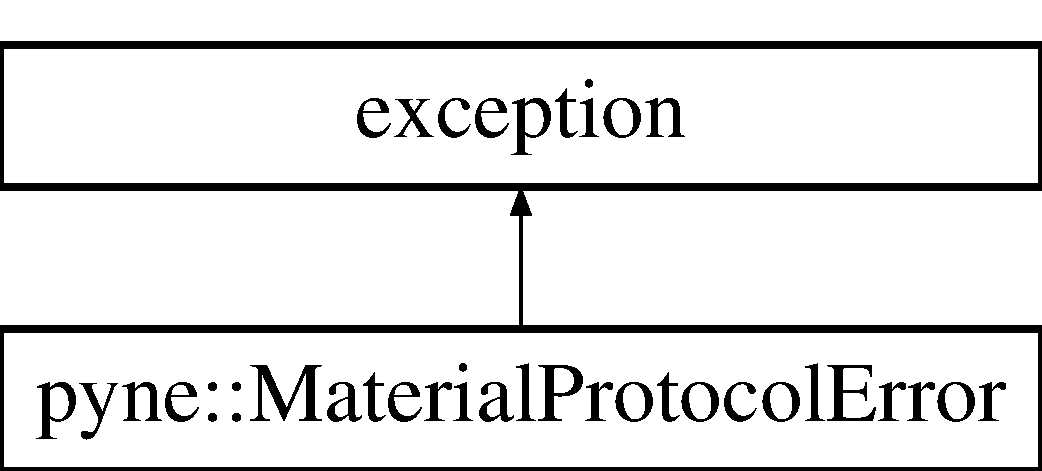
\includegraphics[height=2.000000cm]{classpyne_1_1_material_protocol_error}
\end{center}
\end{figure}


\subsection{Detailed Description}
Custom exception for invalid H\-D\-F5 protocol numbers. 

The documentation for this class was generated from the following file\-:\begin{DoxyCompactItemize}
\item 
/home/scopatz/pyne/src/material.\-h\end{DoxyCompactItemize}

\hypertarget{structtracking__data__structures_1_1meshcell}{\section{tracking\-\_\-data\-\_\-structures\-:\-:meshcell Type Reference}
\label{structtracking__data__structures_1_1meshcell}\index{tracking\-\_\-data\-\_\-structures\-::meshcell@{tracking\-\_\-data\-\_\-structures\-::meshcell}}
}
\subsection*{Public Attributes}
\begin{DoxyCompactItemize}
\item 
\hypertarget{structtracking__data__structures_1_1meshcell_afd4a41c0924cdfa672043dff98383247}{integer {\bfseries xind}}\label{structtracking__data__structures_1_1meshcell_afd4a41c0924cdfa672043dff98383247}

\item 
\hypertarget{structtracking__data__structures_1_1meshcell_aaf221593bf60310472dfdcc78d6c2e79}{integer {\bfseries yind}}\label{structtracking__data__structures_1_1meshcell_aaf221593bf60310472dfdcc78d6c2e79}

\item 
\hypertarget{structtracking__data__structures_1_1meshcell_ae19a4af32e3f12bfa8042da05505aa6e}{integer {\bfseries zind}}\label{structtracking__data__structures_1_1meshcell_ae19a4af32e3f12bfa8042da05505aa6e}

\item 
\hypertarget{structtracking__data__structures_1_1meshcell_a13fcf4021ce5a5d1579ffbff38aaf33d}{real(kind=pr), dimension(3, 8) {\bfseries corners}}\label{structtracking__data__structures_1_1meshcell_a13fcf4021ce5a5d1579ffbff38aaf33d}

\item 
\hypertarget{structtracking__data__structures_1_1meshcell_a4edd8593d1bb0badbc5d723780d2c6c5}{real(kind=pr), dimension(3, 2, 12) {\bfseries edges}}\label{structtracking__data__structures_1_1meshcell_a4edd8593d1bb0badbc5d723780d2c6c5}

\item 
\hypertarget{structtracking__data__structures_1_1meshcell_a8b0a596007ab35b13961d9037d7b6e44}{real(kind=pr), dimension(3, 3, 6) {\bfseries faces}}\label{structtracking__data__structures_1_1meshcell_a8b0a596007ab35b13961d9037d7b6e44}

\item 
\hypertarget{structtracking__data__structures_1_1meshcell_a1a08090e934eae80b9b27f55c4ccaa00}{real(kind=pr) {\bfseries volume}}\label{structtracking__data__structures_1_1meshcell_a1a08090e934eae80b9b27f55c4ccaa00}

\end{DoxyCompactItemize}


The documentation for this type was generated from the following file\-:\begin{DoxyCompactItemize}
\item 
/home/elliott/\-Research/pyne/src/ahot/spatial\-\_\-solvers\-\_\-3d/\-S\-C\-T-\/\-Step/src\-\_\-ahotn-\/step-\/sct/trackstruct.\-f90\end{DoxyCompactItemize}

\hypertarget{structpyne_1_1ndsfpy}{\section{pyne\-:\-:ndsfpy Struct Reference}
\label{structpyne_1_1ndsfpy}\index{pyne\-::ndsfpy@{pyne\-::ndsfpy}}
}


a struct matching the '/neutron/nds\-\_\-fission\-\_\-product' table in nuc\-\_\-data.\-h5  




{\ttfamily \#include $<$data.\-h$>$}

\subsection*{Public Attributes}
\begin{DoxyCompactItemize}
\item 
\hypertarget{structpyne_1_1ndsfpy_ad2cb8c35a387624f95c5318f259834db}{int \hyperlink{structpyne_1_1ndsfpy_ad2cb8c35a387624f95c5318f259834db}{from\-\_\-nuc}}\label{structpyne_1_1ndsfpy_ad2cb8c35a387624f95c5318f259834db}

\begin{DoxyCompactList}\small\item\em id of fissioning nuclide \end{DoxyCompactList}\item 
\hypertarget{structpyne_1_1ndsfpy_aeabd96ca1b30be7381853ca0ccd75f31}{int \hyperlink{structpyne_1_1ndsfpy_aeabd96ca1b30be7381853ca0ccd75f31}{to\-\_\-nuc}}\label{structpyne_1_1ndsfpy_aeabd96ca1b30be7381853ca0ccd75f31}

\begin{DoxyCompactList}\small\item\em id of fission product \end{DoxyCompactList}\item 
\hypertarget{structpyne_1_1ndsfpy_a802ebba1436e6e7ca9595e77698310e8}{double \hyperlink{structpyne_1_1ndsfpy_a802ebba1436e6e7ca9595e77698310e8}{yield\-\_\-thermal}}\label{structpyne_1_1ndsfpy_a802ebba1436e6e7ca9595e77698310e8}

\begin{DoxyCompactList}\small\item\em thermal yield \mbox{[}fraction\mbox{]} \end{DoxyCompactList}\item 
\hypertarget{structpyne_1_1ndsfpy_affaf73e5d64d7e9e94f63c6807b7b17e}{double \hyperlink{structpyne_1_1ndsfpy_affaf73e5d64d7e9e94f63c6807b7b17e}{yield\-\_\-thermal\-\_\-err}}\label{structpyne_1_1ndsfpy_affaf73e5d64d7e9e94f63c6807b7b17e}

\begin{DoxyCompactList}\small\item\em thermal yield error \mbox{[}fraction\mbox{]} \end{DoxyCompactList}\item 
\hypertarget{structpyne_1_1ndsfpy_ae890b10d182d771d0837b24818040a25}{double \hyperlink{structpyne_1_1ndsfpy_ae890b10d182d771d0837b24818040a25}{yield\-\_\-fast}}\label{structpyne_1_1ndsfpy_ae890b10d182d771d0837b24818040a25}

\begin{DoxyCompactList}\small\item\em fast yield \mbox{[}fraction\mbox{]} \end{DoxyCompactList}\item 
\hypertarget{structpyne_1_1ndsfpy_a0e2478bc6cbf2317861727a88cb8370b}{double \hyperlink{structpyne_1_1ndsfpy_a0e2478bc6cbf2317861727a88cb8370b}{yield\-\_\-fast\-\_\-err}}\label{structpyne_1_1ndsfpy_a0e2478bc6cbf2317861727a88cb8370b}

\begin{DoxyCompactList}\small\item\em fast yield error \mbox{[}fraction\mbox{]} \end{DoxyCompactList}\item 
\hypertarget{structpyne_1_1ndsfpy_a5e67e99b97b5ca511ca39c6dcd4b186e}{double \hyperlink{structpyne_1_1ndsfpy_a5e67e99b97b5ca511ca39c6dcd4b186e}{yield\-\_\-14\-Me\-V}}\label{structpyne_1_1ndsfpy_a5e67e99b97b5ca511ca39c6dcd4b186e}

\begin{DoxyCompactList}\small\item\em 14 Me\-V yield \mbox{[}fraction\mbox{]} \end{DoxyCompactList}\item 
\hypertarget{structpyne_1_1ndsfpy_a1d24f4162fe242108b8032f76171d7e5}{double \hyperlink{structpyne_1_1ndsfpy_a1d24f4162fe242108b8032f76171d7e5}{yield\-\_\-14\-Me\-V\-\_\-err}}\label{structpyne_1_1ndsfpy_a1d24f4162fe242108b8032f76171d7e5}

\begin{DoxyCompactList}\small\item\em 14 Me\-V yield error \mbox{[}fraction\mbox{]} \end{DoxyCompactList}\end{DoxyCompactItemize}


\subsection{Detailed Description}
a struct matching the '/neutron/nds\-\_\-fission\-\_\-product' table in nuc\-\_\-data.\-h5 

The documentation for this struct was generated from the following file\-:\begin{DoxyCompactItemize}
\item 
/home/elliott/\-Research/pyne/src/\hyperlink{data_8h}{data.\-h}\end{DoxyCompactItemize}

\hypertarget{structpyne_1_1ndsfpysub}{\section{pyne\-:\-:ndsfpysub Struct Reference}
\label{structpyne_1_1ndsfpysub}\index{pyne\-::ndsfpysub@{pyne\-::ndsfpysub}}
}


a struct for the nds data for fpyield  




{\ttfamily \#include $<$data.\-h$>$}

\subsection*{Public Attributes}
\begin{DoxyCompactItemize}
\item 
\hypertarget{structpyne_1_1ndsfpysub_a83cf4a8733bb234e41c947a21a515cf0}{double \hyperlink{structpyne_1_1ndsfpysub_a83cf4a8733bb234e41c947a21a515cf0}{yield\-\_\-thermal}}\label{structpyne_1_1ndsfpysub_a83cf4a8733bb234e41c947a21a515cf0}

\begin{DoxyCompactList}\small\item\em thermal yield \mbox{[}fraction\mbox{]} \end{DoxyCompactList}\item 
\hypertarget{structpyne_1_1ndsfpysub_a8a95ca96e3cee6ef8a16dcbaf17ca6d3}{double \hyperlink{structpyne_1_1ndsfpysub_a8a95ca96e3cee6ef8a16dcbaf17ca6d3}{yield\-\_\-thermal\-\_\-err}}\label{structpyne_1_1ndsfpysub_a8a95ca96e3cee6ef8a16dcbaf17ca6d3}

\begin{DoxyCompactList}\small\item\em thermal yield error \mbox{[}fraction\mbox{]} \end{DoxyCompactList}\item 
\hypertarget{structpyne_1_1ndsfpysub_acc33c1cd93f9133c15024fa8d4b066dd}{double \hyperlink{structpyne_1_1ndsfpysub_acc33c1cd93f9133c15024fa8d4b066dd}{yield\-\_\-fast}}\label{structpyne_1_1ndsfpysub_acc33c1cd93f9133c15024fa8d4b066dd}

\begin{DoxyCompactList}\small\item\em fast yield \mbox{[}fraction\mbox{]} \end{DoxyCompactList}\item 
\hypertarget{structpyne_1_1ndsfpysub_aa7143b625fe8932ff159b3d9e0030b38}{double \hyperlink{structpyne_1_1ndsfpysub_aa7143b625fe8932ff159b3d9e0030b38}{yield\-\_\-fast\-\_\-err}}\label{structpyne_1_1ndsfpysub_aa7143b625fe8932ff159b3d9e0030b38}

\begin{DoxyCompactList}\small\item\em fast yield error \mbox{[}fraction\mbox{]} \end{DoxyCompactList}\item 
\hypertarget{structpyne_1_1ndsfpysub_afb3737be03fedddc6f54fa3a0e59f0e8}{double \hyperlink{structpyne_1_1ndsfpysub_afb3737be03fedddc6f54fa3a0e59f0e8}{yield\-\_\-14\-Me\-V}}\label{structpyne_1_1ndsfpysub_afb3737be03fedddc6f54fa3a0e59f0e8}

\begin{DoxyCompactList}\small\item\em 14 Me\-V yield \mbox{[}fraction\mbox{]} \end{DoxyCompactList}\item 
\hypertarget{structpyne_1_1ndsfpysub_a7bc2487245689a3f6a095f2254e66e99}{double \hyperlink{structpyne_1_1ndsfpysub_a7bc2487245689a3f6a095f2254e66e99}{yield\-\_\-14\-Me\-V\-\_\-err}}\label{structpyne_1_1ndsfpysub_a7bc2487245689a3f6a095f2254e66e99}

\begin{DoxyCompactList}\small\item\em 14 Me\-V yield error \mbox{[}fraction\mbox{]} \end{DoxyCompactList}\end{DoxyCompactItemize}


\subsection{Detailed Description}
a struct for the nds data for fpyield 

The documentation for this struct was generated from the following file\-:\begin{DoxyCompactItemize}
\item 
/home/elliott/\-Research/pyne/src/\hyperlink{data_8h}{data.\-h}\end{DoxyCompactItemize}

\hypertarget{classpyne_1_1nucname_1_1_not_a_nuclide}{\section{pyne\+:\+:nucname\+:\+:Not\+A\+Nuclide Class Reference}
\label{classpyne_1_1nucname_1_1_not_a_nuclide}\index{pyne\+::nucname\+::\+Not\+A\+Nuclide@{pyne\+::nucname\+::\+Not\+A\+Nuclide}}
}


{\ttfamily \#include $<$nucname.\+h$>$}

Inheritance diagram for pyne\+:\+:nucname\+:\+:Not\+A\+Nuclide\+:\begin{figure}[H]
\begin{center}
\leavevmode
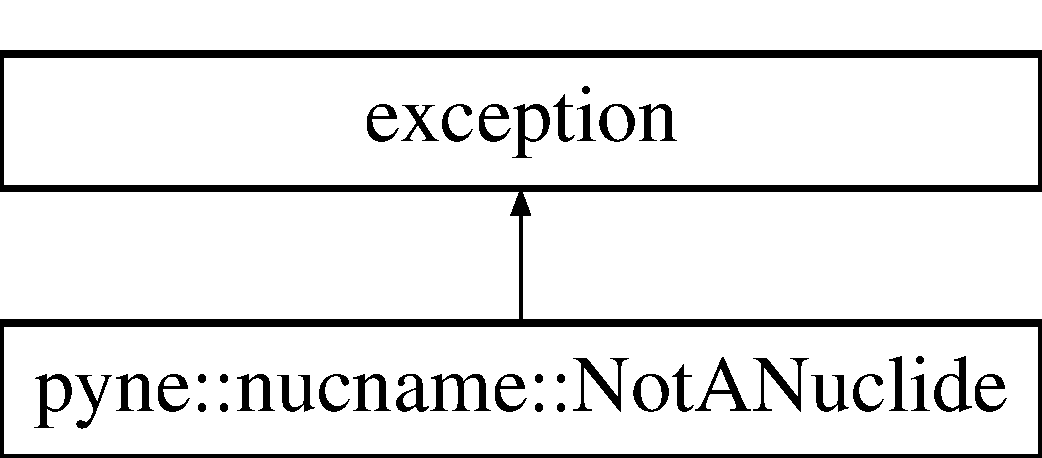
\includegraphics[height=2.000000cm]{classpyne_1_1nucname_1_1_not_a_nuclide}
\end{center}
\end{figure}
\subsection*{Public Member Functions}
\begin{DoxyCompactItemize}
\item 
\hypertarget{classpyne_1_1nucname_1_1_not_a_nuclide_ac1c10c25703f622788f475609fd5eed6}{\hyperlink{classpyne_1_1nucname_1_1_not_a_nuclide_ac1c10c25703f622788f475609fd5eed6}{Not\+A\+Nuclide} ()}\label{classpyne_1_1nucname_1_1_not_a_nuclide_ac1c10c25703f622788f475609fd5eed6}

\begin{DoxyCompactList}\small\item\em default constructor \end{DoxyCompactList}\item 
\hypertarget{classpyne_1_1nucname_1_1_not_a_nuclide_a2fd948fc4d3be06a456b30188944b88a}{\hyperlink{classpyne_1_1nucname_1_1_not_a_nuclide_a2fd948fc4d3be06a456b30188944b88a}{$\sim$\+Not\+A\+Nuclide} ()  throw ()}\label{classpyne_1_1nucname_1_1_not_a_nuclide_a2fd948fc4d3be06a456b30188944b88a}

\begin{DoxyCompactList}\small\item\em default destructor \end{DoxyCompactList}\item 
\hyperlink{classpyne_1_1nucname_1_1_not_a_nuclide_a32741575cb99d294d54f39bc4ca5e51c}{Not\+A\+Nuclide} (std\+::string wasptr, std\+::string nowptr)
\item 
\hyperlink{classpyne_1_1nucname_1_1_not_a_nuclide_a10f9f9c4be5b439f1dafd1450943252d}{Not\+A\+Nuclide} (std\+::string wasptr, int nowptr)
\item 
\hyperlink{classpyne_1_1nucname_1_1_not_a_nuclide_af8665194481f65e932cbd4244ee636ae}{Not\+A\+Nuclide} (int wasptr, std\+::string nowptr)
\item 
\hyperlink{classpyne_1_1nucname_1_1_not_a_nuclide_adbc9b62fa21ec1ab4957ca8a4569a8c6}{Not\+A\+Nuclide} (int wasptr, int nowptr)
\item 
virtual const char $\ast$ \hyperlink{classpyne_1_1nucname_1_1_not_a_nuclide_adb841d59149843b5b5718f5ccc47b4dc}{what} () const   throw ()
\end{DoxyCompactItemize}


\subsection{Detailed Description}
Custom expection for declaring that a value does not follow a recognizable nuclide naming convention. 

\subsection{Constructor \& Destructor Documentation}
\hypertarget{classpyne_1_1nucname_1_1_not_a_nuclide_a32741575cb99d294d54f39bc4ca5e51c}{\index{pyne\+::nucname\+::\+Not\+A\+Nuclide@{pyne\+::nucname\+::\+Not\+A\+Nuclide}!Not\+A\+Nuclide@{Not\+A\+Nuclide}}
\index{Not\+A\+Nuclide@{Not\+A\+Nuclide}!pyne\+::nucname\+::\+Not\+A\+Nuclide@{pyne\+::nucname\+::\+Not\+A\+Nuclide}}
\subsubsection[{Not\+A\+Nuclide}]{\setlength{\rightskip}{0pt plus 5cm}pyne\+::nucname\+::\+Not\+A\+Nuclide\+::\+Not\+A\+Nuclide (
\begin{DoxyParamCaption}
\item[{std\+::string}]{wasptr, }
\item[{std\+::string}]{nowptr}
\end{DoxyParamCaption}
)\hspace{0.3cm}{\ttfamily [inline]}}}\label{classpyne_1_1nucname_1_1_not_a_nuclide_a32741575cb99d294d54f39bc4ca5e51c}
Constructor given previous and current state of nulide name 
\begin{DoxyParams}{Parameters}
{\em wasptr} & Previous state, typically user input. \\
\hline
{\em nowptr} & Current state, as far as Py\+N\+E could get. \\
\hline
\end{DoxyParams}
\hypertarget{classpyne_1_1nucname_1_1_not_a_nuclide_a10f9f9c4be5b439f1dafd1450943252d}{\index{pyne\+::nucname\+::\+Not\+A\+Nuclide@{pyne\+::nucname\+::\+Not\+A\+Nuclide}!Not\+A\+Nuclide@{Not\+A\+Nuclide}}
\index{Not\+A\+Nuclide@{Not\+A\+Nuclide}!pyne\+::nucname\+::\+Not\+A\+Nuclide@{pyne\+::nucname\+::\+Not\+A\+Nuclide}}
\subsubsection[{Not\+A\+Nuclide}]{\setlength{\rightskip}{0pt plus 5cm}pyne\+::nucname\+::\+Not\+A\+Nuclide\+::\+Not\+A\+Nuclide (
\begin{DoxyParamCaption}
\item[{std\+::string}]{wasptr, }
\item[{int}]{nowptr}
\end{DoxyParamCaption}
)\hspace{0.3cm}{\ttfamily [inline]}}}\label{classpyne_1_1nucname_1_1_not_a_nuclide_a10f9f9c4be5b439f1dafd1450943252d}
Constructor given previous and current state of nulide name 
\begin{DoxyParams}{Parameters}
{\em wasptr} & Previous state, typically user input. \\
\hline
{\em nowptr} & Current state, as far as Py\+N\+E could get. \\
\hline
\end{DoxyParams}
\hypertarget{classpyne_1_1nucname_1_1_not_a_nuclide_af8665194481f65e932cbd4244ee636ae}{\index{pyne\+::nucname\+::\+Not\+A\+Nuclide@{pyne\+::nucname\+::\+Not\+A\+Nuclide}!Not\+A\+Nuclide@{Not\+A\+Nuclide}}
\index{Not\+A\+Nuclide@{Not\+A\+Nuclide}!pyne\+::nucname\+::\+Not\+A\+Nuclide@{pyne\+::nucname\+::\+Not\+A\+Nuclide}}
\subsubsection[{Not\+A\+Nuclide}]{\setlength{\rightskip}{0pt plus 5cm}pyne\+::nucname\+::\+Not\+A\+Nuclide\+::\+Not\+A\+Nuclide (
\begin{DoxyParamCaption}
\item[{int}]{wasptr, }
\item[{std\+::string}]{nowptr}
\end{DoxyParamCaption}
)\hspace{0.3cm}{\ttfamily [inline]}}}\label{classpyne_1_1nucname_1_1_not_a_nuclide_af8665194481f65e932cbd4244ee636ae}
Constructor given previous and current state of nulide name 
\begin{DoxyParams}{Parameters}
{\em wasptr} & Previous state, typically user input. \\
\hline
{\em nowptr} & Current state, as far as Py\+N\+E could get. \\
\hline
\end{DoxyParams}
\hypertarget{classpyne_1_1nucname_1_1_not_a_nuclide_adbc9b62fa21ec1ab4957ca8a4569a8c6}{\index{pyne\+::nucname\+::\+Not\+A\+Nuclide@{pyne\+::nucname\+::\+Not\+A\+Nuclide}!Not\+A\+Nuclide@{Not\+A\+Nuclide}}
\index{Not\+A\+Nuclide@{Not\+A\+Nuclide}!pyne\+::nucname\+::\+Not\+A\+Nuclide@{pyne\+::nucname\+::\+Not\+A\+Nuclide}}
\subsubsection[{Not\+A\+Nuclide}]{\setlength{\rightskip}{0pt plus 5cm}pyne\+::nucname\+::\+Not\+A\+Nuclide\+::\+Not\+A\+Nuclide (
\begin{DoxyParamCaption}
\item[{int}]{wasptr, }
\item[{int}]{nowptr}
\end{DoxyParamCaption}
)\hspace{0.3cm}{\ttfamily [inline]}}}\label{classpyne_1_1nucname_1_1_not_a_nuclide_adbc9b62fa21ec1ab4957ca8a4569a8c6}
Constructor given previous and current state of nulide name 
\begin{DoxyParams}{Parameters}
{\em wasptr} & Previous state, typically user input. \\
\hline
{\em nowptr} & Current state, as far as Py\+N\+E could get. \\
\hline
\end{DoxyParams}


\subsection{Member Function Documentation}
\hypertarget{classpyne_1_1nucname_1_1_not_a_nuclide_adb841d59149843b5b5718f5ccc47b4dc}{\index{pyne\+::nucname\+::\+Not\+A\+Nuclide@{pyne\+::nucname\+::\+Not\+A\+Nuclide}!what@{what}}
\index{what@{what}!pyne\+::nucname\+::\+Not\+A\+Nuclide@{pyne\+::nucname\+::\+Not\+A\+Nuclide}}
\subsubsection[{what}]{\setlength{\rightskip}{0pt plus 5cm}virtual const char$\ast$ pyne\+::nucname\+::\+Not\+A\+Nuclide\+::what (
\begin{DoxyParamCaption}
{}
\end{DoxyParamCaption}
) const throw  ) \hspace{0.3cm}{\ttfamily [inline]}, {\ttfamily [virtual]}}}\label{classpyne_1_1nucname_1_1_not_a_nuclide_adb841d59149843b5b5718f5ccc47b4dc}
Generates an informational message for the exception \begin{DoxyReturn}{Returns}
The error string 
\end{DoxyReturn}


The documentation for this class was generated from the following file\+:\begin{DoxyCompactItemize}
\item 
/\+Users/bates26/\+Documents/pyne/src/nucname.\+h\end{DoxyCompactItemize}

\hypertarget{classpyne_1_1particle_1_1_not_a_particle}{\section{pyne\-:\-:particle\-:\-:Not\-A\-Particle Class Reference}
\label{classpyne_1_1particle_1_1_not_a_particle}\index{pyne\-::particle\-::\-Not\-A\-Particle@{pyne\-::particle\-::\-Not\-A\-Particle}}
}


Custom excpeption for failed particle types.  




{\ttfamily \#include $<$particle.\-h$>$}

Inheritance diagram for pyne\-:\-:particle\-:\-:Not\-A\-Particle\-:\begin{figure}[H]
\begin{center}
\leavevmode
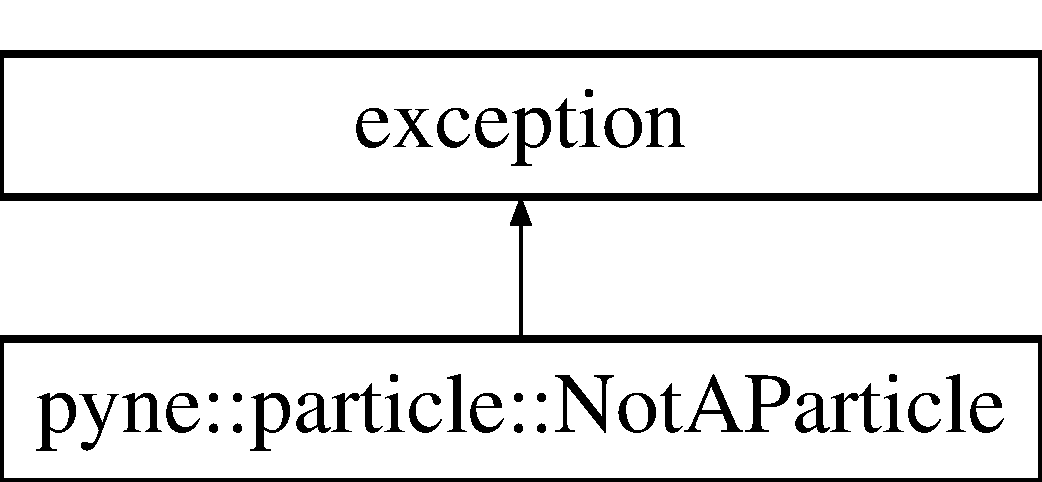
\includegraphics[height=2.000000cm]{classpyne_1_1particle_1_1_not_a_particle}
\end{center}
\end{figure}
\subsection*{Public Member Functions}
\begin{DoxyCompactItemize}
\item 
\hypertarget{classpyne_1_1particle_1_1_not_a_particle_af98a293003d5e5a570685c5985b7c501}{\hyperlink{classpyne_1_1particle_1_1_not_a_particle_af98a293003d5e5a570685c5985b7c501}{Not\-A\-Particle} ()}\label{classpyne_1_1particle_1_1_not_a_particle_af98a293003d5e5a570685c5985b7c501}

\begin{DoxyCompactList}\small\item\em Default constructor. \end{DoxyCompactList}\item 
\hypertarget{classpyne_1_1particle_1_1_not_a_particle_abe61e24b09e9846161bc264a1dc7978d}{\hyperlink{classpyne_1_1particle_1_1_not_a_particle_abe61e24b09e9846161bc264a1dc7978d}{$\sim$\-Not\-A\-Particle} ()  throw ()}\label{classpyne_1_1particle_1_1_not_a_particle_abe61e24b09e9846161bc264a1dc7978d}

\begin{DoxyCompactList}\small\item\em Default destructor. \end{DoxyCompactList}\item 
\hyperlink{classpyne_1_1particle_1_1_not_a_particle_a556fb7c90fc5e4c6ea1c394a86746fc9}{Not\-A\-Particle} (std\-::string particle\-\_\-name)
\item 
\hypertarget{classpyne_1_1particle_1_1_not_a_particle_a70a50ceb3e0920b45acb4e779865b9db}{virtual const char $\ast$ \hyperlink{classpyne_1_1particle_1_1_not_a_particle_a70a50ceb3e0920b45acb4e779865b9db}{what} () const   throw ()}\label{classpyne_1_1particle_1_1_not_a_particle_a70a50ceb3e0920b45acb4e779865b9db}

\begin{DoxyCompactList}\small\item\em raises error message \end{DoxyCompactList}\end{DoxyCompactItemize}


\subsection{Detailed Description}
Custom excpeption for failed particle types. 

\subsection{Constructor \& Destructor Documentation}
\hypertarget{classpyne_1_1particle_1_1_not_a_particle_a556fb7c90fc5e4c6ea1c394a86746fc9}{\index{pyne\-::particle\-::\-Not\-A\-Particle@{pyne\-::particle\-::\-Not\-A\-Particle}!Not\-A\-Particle@{Not\-A\-Particle}}
\index{Not\-A\-Particle@{Not\-A\-Particle}!pyne::particle::NotAParticle@{pyne\-::particle\-::\-Not\-A\-Particle}}
\subsubsection[{Not\-A\-Particle}]{\setlength{\rightskip}{0pt plus 5cm}pyne\-::particle\-::\-Not\-A\-Particle\-::\-Not\-A\-Particle (
\begin{DoxyParamCaption}
\item[{std\-::string}]{particle\-\_\-name}
\end{DoxyParamCaption}
)\hspace{0.3cm}{\ttfamily [inline]}}}\label{classpyne_1_1particle_1_1_not_a_particle_a556fb7c90fc5e4c6ea1c394a86746fc9}
Constructor for raising the exception Spits out the particle name as input 

The documentation for this class was generated from the following file\-:\begin{DoxyCompactItemize}
\item 
/home/elliott/\-Research/pyne/src/particle.\-h\end{DoxyCompactItemize}

\hypertarget{classpyne_1_1rxname_1_1_not_a_reaction}{\section{pyne\-:\-:rxname\-:\-:Not\-A\-Reaction Class Reference}
\label{classpyne_1_1rxname_1_1_not_a_reaction}\index{pyne\-::rxname\-::\-Not\-A\-Reaction@{pyne\-::rxname\-::\-Not\-A\-Reaction}}
}


Custom exception for declaring a value not to be a valid reaction.  




{\ttfamily \#include $<$rxname.\-h$>$}

Inheritance diagram for pyne\-:\-:rxname\-:\-:Not\-A\-Reaction\-:\begin{figure}[H]
\begin{center}
\leavevmode
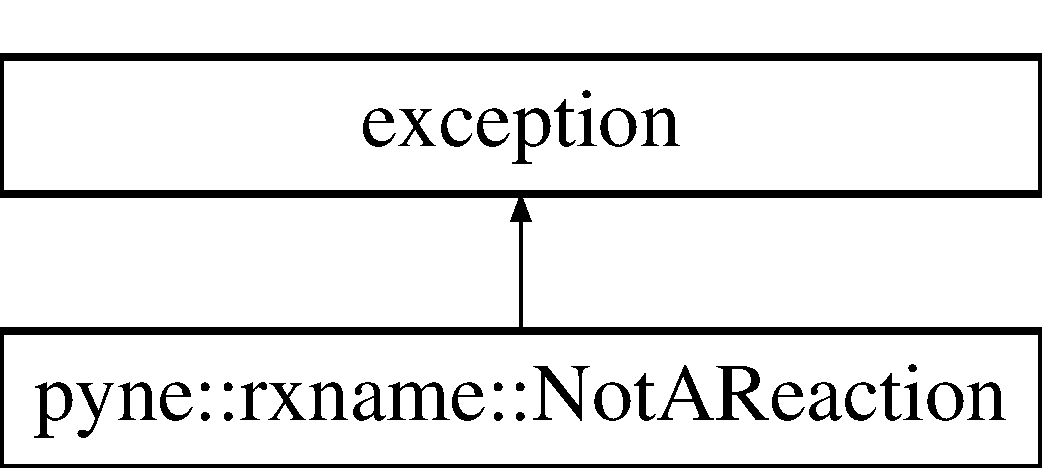
\includegraphics[height=2.000000cm]{classpyne_1_1rxname_1_1_not_a_reaction}
\end{center}
\end{figure}
\subsection*{Public Member Functions}
\begin{DoxyCompactItemize}
\item 
\hypertarget{classpyne_1_1rxname_1_1_not_a_reaction_abb889337afdab53c131adf5702fb16d0}{\hyperlink{classpyne_1_1rxname_1_1_not_a_reaction_abb889337afdab53c131adf5702fb16d0}{Not\-A\-Reaction} ()}\label{classpyne_1_1rxname_1_1_not_a_reaction_abb889337afdab53c131adf5702fb16d0}

\begin{DoxyCompactList}\small\item\em default constructor \end{DoxyCompactList}\item 
\hypertarget{classpyne_1_1rxname_1_1_not_a_reaction_a2a34cc0de45875c17c004acff20dc535}{\hyperlink{classpyne_1_1rxname_1_1_not_a_reaction_a2a34cc0de45875c17c004acff20dc535}{$\sim$\-Not\-A\-Reaction} ()  throw ()}\label{classpyne_1_1rxname_1_1_not_a_reaction_a2a34cc0de45875c17c004acff20dc535}

\begin{DoxyCompactList}\small\item\em default destructor \end{DoxyCompactList}\item 
\hyperlink{classpyne_1_1rxname_1_1_not_a_reaction_a64f23630722811847d030ae0358f959f}{Not\-A\-Reaction} (std\-::string wasptr, std\-::string nowptr)
\item 
\hyperlink{classpyne_1_1rxname_1_1_not_a_reaction_a32de94daecf33a00055c8ac7ada718d7}{Not\-A\-Reaction} (std\-::string wasptr, int nowptr)
\item 
\hyperlink{classpyne_1_1rxname_1_1_not_a_reaction_a828c48bf08dd96121ec83c6cced3063b}{Not\-A\-Reaction} (int wasptr, std\-::string nowptr)
\item 
\hyperlink{classpyne_1_1rxname_1_1_not_a_reaction_a8d16f260eab4fbbc7a5a14b48ce5580d}{Not\-A\-Reaction} (int wasptr, int nowptr)
\item 
\hyperlink{classpyne_1_1rxname_1_1_not_a_reaction_a9f3cea1e2ffd856bd3111569482244d2}{Not\-A\-Reaction} (std\-::string wasptr, unsigned int nowptr)
\item 
\hyperlink{classpyne_1_1rxname_1_1_not_a_reaction_ab5ff27c0ce93ac29da63ab32e7fa44e3}{Not\-A\-Reaction} (unsigned int wasptr, std\-::string nowptr)
\item 
\hyperlink{classpyne_1_1rxname_1_1_not_a_reaction_a7e0b63801e38b5d2c59edd635817fb80}{Not\-A\-Reaction} (unsigned int wasptr, unsigned int nowptr)
\item 
\hypertarget{classpyne_1_1rxname_1_1_not_a_reaction_a82bd7ddf78f0065338ec546dfacf5b45}{virtual const char $\ast$ \hyperlink{classpyne_1_1rxname_1_1_not_a_reaction_a82bd7ddf78f0065338ec546dfacf5b45}{what} () const   throw ()}\label{classpyne_1_1rxname_1_1_not_a_reaction_a82bd7ddf78f0065338ec546dfacf5b45}

\begin{DoxyCompactList}\small\item\em Returns a helpful error message containing prior and current reaction state. \end{DoxyCompactList}\end{DoxyCompactItemize}


\subsection{Detailed Description}
Custom exception for declaring a value not to be a valid reaction. 

\subsection{Constructor \& Destructor Documentation}
\hypertarget{classpyne_1_1rxname_1_1_not_a_reaction_a64f23630722811847d030ae0358f959f}{\index{pyne\-::rxname\-::\-Not\-A\-Reaction@{pyne\-::rxname\-::\-Not\-A\-Reaction}!Not\-A\-Reaction@{Not\-A\-Reaction}}
\index{Not\-A\-Reaction@{Not\-A\-Reaction}!pyne::rxname::NotAReaction@{pyne\-::rxname\-::\-Not\-A\-Reaction}}
\subsubsection[{Not\-A\-Reaction}]{\setlength{\rightskip}{0pt plus 5cm}pyne\-::rxname\-::\-Not\-A\-Reaction\-::\-Not\-A\-Reaction (
\begin{DoxyParamCaption}
\item[{std\-::string}]{wasptr, }
\item[{std\-::string}]{nowptr}
\end{DoxyParamCaption}
)\hspace{0.3cm}{\ttfamily [inline]}}}\label{classpyne_1_1rxname_1_1_not_a_reaction_a64f23630722811847d030ae0358f959f}
Constructor using original reaction ({\itshape wasptr}) and the eventual state that Py\-N\-E calculated ({\itshape nowptr}). \hypertarget{classpyne_1_1rxname_1_1_not_a_reaction_a32de94daecf33a00055c8ac7ada718d7}{\index{pyne\-::rxname\-::\-Not\-A\-Reaction@{pyne\-::rxname\-::\-Not\-A\-Reaction}!Not\-A\-Reaction@{Not\-A\-Reaction}}
\index{Not\-A\-Reaction@{Not\-A\-Reaction}!pyne::rxname::NotAReaction@{pyne\-::rxname\-::\-Not\-A\-Reaction}}
\subsubsection[{Not\-A\-Reaction}]{\setlength{\rightskip}{0pt plus 5cm}pyne\-::rxname\-::\-Not\-A\-Reaction\-::\-Not\-A\-Reaction (
\begin{DoxyParamCaption}
\item[{std\-::string}]{wasptr, }
\item[{int}]{nowptr}
\end{DoxyParamCaption}
)\hspace{0.3cm}{\ttfamily [inline]}}}\label{classpyne_1_1rxname_1_1_not_a_reaction_a32de94daecf33a00055c8ac7ada718d7}
Constructor using original reaction ({\itshape wasptr}) and the eventual state that Py\-N\-E calculated ({\itshape nowptr}). \hypertarget{classpyne_1_1rxname_1_1_not_a_reaction_a828c48bf08dd96121ec83c6cced3063b}{\index{pyne\-::rxname\-::\-Not\-A\-Reaction@{pyne\-::rxname\-::\-Not\-A\-Reaction}!Not\-A\-Reaction@{Not\-A\-Reaction}}
\index{Not\-A\-Reaction@{Not\-A\-Reaction}!pyne::rxname::NotAReaction@{pyne\-::rxname\-::\-Not\-A\-Reaction}}
\subsubsection[{Not\-A\-Reaction}]{\setlength{\rightskip}{0pt plus 5cm}pyne\-::rxname\-::\-Not\-A\-Reaction\-::\-Not\-A\-Reaction (
\begin{DoxyParamCaption}
\item[{int}]{wasptr, }
\item[{std\-::string}]{nowptr}
\end{DoxyParamCaption}
)\hspace{0.3cm}{\ttfamily [inline]}}}\label{classpyne_1_1rxname_1_1_not_a_reaction_a828c48bf08dd96121ec83c6cced3063b}
Constructor using original reaction ({\itshape wasptr}) and the eventual state that Py\-N\-E calculated ({\itshape nowptr}). \hypertarget{classpyne_1_1rxname_1_1_not_a_reaction_a8d16f260eab4fbbc7a5a14b48ce5580d}{\index{pyne\-::rxname\-::\-Not\-A\-Reaction@{pyne\-::rxname\-::\-Not\-A\-Reaction}!Not\-A\-Reaction@{Not\-A\-Reaction}}
\index{Not\-A\-Reaction@{Not\-A\-Reaction}!pyne::rxname::NotAReaction@{pyne\-::rxname\-::\-Not\-A\-Reaction}}
\subsubsection[{Not\-A\-Reaction}]{\setlength{\rightskip}{0pt plus 5cm}pyne\-::rxname\-::\-Not\-A\-Reaction\-::\-Not\-A\-Reaction (
\begin{DoxyParamCaption}
\item[{int}]{wasptr, }
\item[{int}]{nowptr}
\end{DoxyParamCaption}
)\hspace{0.3cm}{\ttfamily [inline]}}}\label{classpyne_1_1rxname_1_1_not_a_reaction_a8d16f260eab4fbbc7a5a14b48ce5580d}
Constructor using original reaction ({\itshape wasptr}) and the eventual state that Py\-N\-E calculated ({\itshape nowptr}). \hypertarget{classpyne_1_1rxname_1_1_not_a_reaction_a9f3cea1e2ffd856bd3111569482244d2}{\index{pyne\-::rxname\-::\-Not\-A\-Reaction@{pyne\-::rxname\-::\-Not\-A\-Reaction}!Not\-A\-Reaction@{Not\-A\-Reaction}}
\index{Not\-A\-Reaction@{Not\-A\-Reaction}!pyne::rxname::NotAReaction@{pyne\-::rxname\-::\-Not\-A\-Reaction}}
\subsubsection[{Not\-A\-Reaction}]{\setlength{\rightskip}{0pt plus 5cm}pyne\-::rxname\-::\-Not\-A\-Reaction\-::\-Not\-A\-Reaction (
\begin{DoxyParamCaption}
\item[{std\-::string}]{wasptr, }
\item[{unsigned int}]{nowptr}
\end{DoxyParamCaption}
)\hspace{0.3cm}{\ttfamily [inline]}}}\label{classpyne_1_1rxname_1_1_not_a_reaction_a9f3cea1e2ffd856bd3111569482244d2}
Constructor using original reaction ({\itshape wasptr}) and the eventual state that Py\-N\-E calculated ({\itshape nowptr}). \hypertarget{classpyne_1_1rxname_1_1_not_a_reaction_ab5ff27c0ce93ac29da63ab32e7fa44e3}{\index{pyne\-::rxname\-::\-Not\-A\-Reaction@{pyne\-::rxname\-::\-Not\-A\-Reaction}!Not\-A\-Reaction@{Not\-A\-Reaction}}
\index{Not\-A\-Reaction@{Not\-A\-Reaction}!pyne::rxname::NotAReaction@{pyne\-::rxname\-::\-Not\-A\-Reaction}}
\subsubsection[{Not\-A\-Reaction}]{\setlength{\rightskip}{0pt plus 5cm}pyne\-::rxname\-::\-Not\-A\-Reaction\-::\-Not\-A\-Reaction (
\begin{DoxyParamCaption}
\item[{unsigned int}]{wasptr, }
\item[{std\-::string}]{nowptr}
\end{DoxyParamCaption}
)\hspace{0.3cm}{\ttfamily [inline]}}}\label{classpyne_1_1rxname_1_1_not_a_reaction_ab5ff27c0ce93ac29da63ab32e7fa44e3}
Constructor using original reaction ({\itshape wasptr}) and the eventual state that Py\-N\-E calculated ({\itshape nowptr}). \hypertarget{classpyne_1_1rxname_1_1_not_a_reaction_a7e0b63801e38b5d2c59edd635817fb80}{\index{pyne\-::rxname\-::\-Not\-A\-Reaction@{pyne\-::rxname\-::\-Not\-A\-Reaction}!Not\-A\-Reaction@{Not\-A\-Reaction}}
\index{Not\-A\-Reaction@{Not\-A\-Reaction}!pyne::rxname::NotAReaction@{pyne\-::rxname\-::\-Not\-A\-Reaction}}
\subsubsection[{Not\-A\-Reaction}]{\setlength{\rightskip}{0pt plus 5cm}pyne\-::rxname\-::\-Not\-A\-Reaction\-::\-Not\-A\-Reaction (
\begin{DoxyParamCaption}
\item[{unsigned int}]{wasptr, }
\item[{unsigned int}]{nowptr}
\end{DoxyParamCaption}
)\hspace{0.3cm}{\ttfamily [inline]}}}\label{classpyne_1_1rxname_1_1_not_a_reaction_a7e0b63801e38b5d2c59edd635817fb80}
Constructor using original reaction ({\itshape wasptr}) and the eventual state that Py\-N\-E calculated ({\itshape nowptr}). 

The documentation for this class was generated from the following file\-:\begin{DoxyCompactItemize}
\item 
/home/elliott/\-Research/pyne/src/rxname.\-h\end{DoxyCompactItemize}

\hypertarget{classh5wrap_1_1_path_not_found}{\section{h5wrap\-:\-:Path\-Not\-Found Class Reference}
\label{classh5wrap_1_1_path_not_found}\index{h5wrap\-::\-Path\-Not\-Found@{h5wrap\-::\-Path\-Not\-Found}}
}


Custom exception for when a path is not found in an H\-D\-F5 file.  




{\ttfamily \#include $<$h5wrap.\-h$>$}

Inheritance diagram for h5wrap\-:\-:Path\-Not\-Found\-:\begin{figure}[H]
\begin{center}
\leavevmode
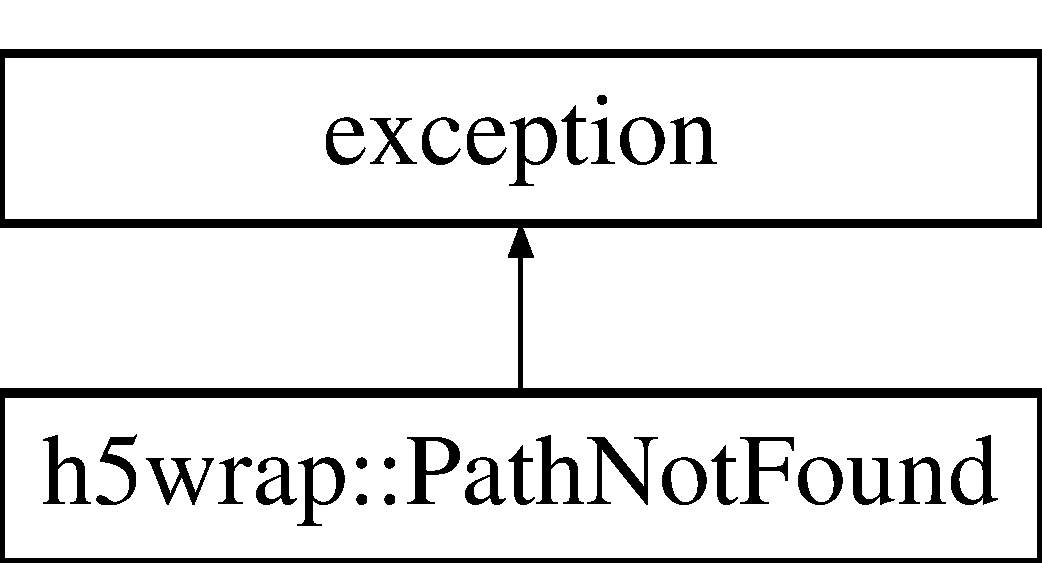
\includegraphics[height=2.000000cm]{classh5wrap_1_1_path_not_found}
\end{center}
\end{figure}
\subsection*{Public Member Functions}
\begin{DoxyCompactItemize}
\item 
\hypertarget{classh5wrap_1_1_path_not_found_a7b05229fb4f02920732f22622af1f08e}{\hyperlink{classh5wrap_1_1_path_not_found_a7b05229fb4f02920732f22622af1f08e}{Path\-Not\-Found} ()}\label{classh5wrap_1_1_path_not_found_a7b05229fb4f02920732f22622af1f08e}

\begin{DoxyCompactList}\small\item\em default constructor \end{DoxyCompactList}\item 
\hypertarget{classh5wrap_1_1_path_not_found_acf9696ccdfb4a4c63454dbfc1dcde060}{\hyperlink{classh5wrap_1_1_path_not_found_acf9696ccdfb4a4c63454dbfc1dcde060}{$\sim$\-Path\-Not\-Found} ()  throw ()}\label{classh5wrap_1_1_path_not_found_acf9696ccdfb4a4c63454dbfc1dcde060}

\begin{DoxyCompactList}\small\item\em default destructor \end{DoxyCompactList}\item 
\hypertarget{classh5wrap_1_1_path_not_found_aaedd26703acced17206eb8dabd4c5274}{\hyperlink{classh5wrap_1_1_path_not_found_aaedd26703acced17206eb8dabd4c5274}{Path\-Not\-Found} (std\-::string fname, std\-::string pname)}\label{classh5wrap_1_1_path_not_found_aaedd26703acced17206eb8dabd4c5274}

\begin{DoxyCompactList}\small\item\em constructor with the filename and the pathname \end{DoxyCompactList}\item 
\hypertarget{classh5wrap_1_1_path_not_found_ad454d14e0f9f44f4357a5c33a7017b88}{virtual const char $\ast$ \hyperlink{classh5wrap_1_1_path_not_found_ad454d14e0f9f44f4357a5c33a7017b88}{what} () const   throw ()}\label{classh5wrap_1_1_path_not_found_ad454d14e0f9f44f4357a5c33a7017b88}

\begin{DoxyCompactList}\small\item\em helpful error message that includes the filename and the pathname \end{DoxyCompactList}\end{DoxyCompactItemize}


\subsection{Detailed Description}
Custom exception for when a path is not found in an H\-D\-F5 file. 

The documentation for this class was generated from the following file\-:\begin{DoxyCompactItemize}
\item 
/home/scopatz/pyne/src/\hyperlink{h5wrap_8h}{h5wrap.\-h}\end{DoxyCompactItemize}

\hypertarget{structsct__module_1_1polyhedron}{\section{sct\-\_\-module\-:\-:polyhedron Type Reference}
\label{structsct__module_1_1polyhedron}\index{sct\-\_\-module\-::polyhedron@{sct\-\_\-module\-::polyhedron}}
}
\subsection*{Public Attributes}
\begin{DoxyCompactItemize}
\item 
\hypertarget{structsct__module_1_1polyhedron_a0a9f5f4cc18647a9ebeb2318bc83dfa7}{integer, dimension(3) {\bfseries indx}}\label{structsct__module_1_1polyhedron_a0a9f5f4cc18647a9ebeb2318bc83dfa7}

\item 
\hypertarget{structsct__module_1_1polyhedron_afc1244f7652724346f6ce31ff39214c3}{real(kind=8) {\bfseries volume}}\label{structsct__module_1_1polyhedron_afc1244f7652724346f6ce31ff39214c3}

\item 
\hypertarget{structsct__module_1_1polyhedron_ad7c601a870a982c8a0b30bd2ee3b1427}{real(kind=8), dimension(-\/3\-:3) {\bfseries area}}\label{structsct__module_1_1polyhedron_ad7c601a870a982c8a0b30bd2ee3b1427}

\item 
\hypertarget{structsct__module_1_1polyhedron_a4d8b6322e32640812e3c917645febc0b}{integer(kind=1), dimension(-\/3\-:3) {\bfseries area\-\_\-exist}}\label{structsct__module_1_1polyhedron_a4d8b6322e32640812e3c917645febc0b}

\end{DoxyCompactItemize}


The documentation for this type was generated from the following file\-:\begin{DoxyCompactItemize}
\item 
/home/elliott/\-Research/pyne/src/ahot/spatial\-\_\-solvers\-\_\-3d/\-S\-C\-T-\/\-Step/src\-\_\-ahotn-\/step-\/sct/sct\-\_\-module.\-f90\end{DoxyCompactItemize}

\hypertarget{classprecision__module}{\section{precision\-\_\-module Module Reference}
\label{classprecision__module}\index{precision\-\_\-module@{precision\-\_\-module}}
}
\subsection*{Public Attributes}
\begin{DoxyCompactItemize}
\item 
\hypertarget{classprecision__module_a666769eb09991cb5f073620c9042674e}{integer, parameter {\bfseries pr} = selected\-\_\-real\-\_\-kind(32, 4000)}\label{classprecision__module_a666769eb09991cb5f073620c9042674e}

\item 
\hypertarget{classprecision__module_af1c73fb151b9820e507052293ef6e4bf}{real(kind=pr), parameter {\bfseries eps} = 1.\-0\-E-\/14\-\_\-pr}\label{classprecision__module_af1c73fb151b9820e507052293ef6e4bf}

\item 
\hypertarget{classprecision__module_a0e5314b479911716c1a708ef3ffe4aa9}{real(kind=pr), parameter {\bfseries peps} = 1.\-8\-E-\/14\-\_\-pr}\label{classprecision__module_a0e5314b479911716c1a708ef3ffe4aa9}

\item 
\hypertarget{classprecision__module_a5c4729f5ae76a54c36ac15655ce815ef}{real(kind=pr), parameter {\bfseries zero} = 0.\-0\-\_\-pr}\label{classprecision__module_a5c4729f5ae76a54c36ac15655ce815ef}

\item 
\hypertarget{classprecision__module_a9985a1c3ada8b0f360aecd58a7da0209}{real(kind=pr), parameter {\bfseries one} = 1.\-0\-\_\-pr}\label{classprecision__module_a9985a1c3ada8b0f360aecd58a7da0209}

\item 
\hypertarget{classprecision__module_a97a3cf9023f43607709fcf9f79f4cf2d}{real(kind=pr), parameter {\bfseries two} = 2.\-0\-\_\-pr}\label{classprecision__module_a97a3cf9023f43607709fcf9f79f4cf2d}

\item 
\hypertarget{classprecision__module_a974fae5c7034e0f3942510dd7f07c50c}{real(kind=pr), parameter {\bfseries three} = 3.\-0\-\_\-pr}\label{classprecision__module_a974fae5c7034e0f3942510dd7f07c50c}

\item 
\hypertarget{classprecision__module_af213aa02e1e91ee1be1e7f9d6ebf1ffc}{real(kind=pr), parameter {\bfseries four} = 4.\-0\-\_\-pr}\label{classprecision__module_af213aa02e1e91ee1be1e7f9d6ebf1ffc}

\item 
\hypertarget{classprecision__module_a2975299bd4cad0c5fc29b217c7a3c55a}{real(kind=pr), parameter {\bfseries half} = 0.\-5\-\_\-pr}\label{classprecision__module_a2975299bd4cad0c5fc29b217c7a3c55a}

\item 
\hypertarget{classprecision__module_a0517b994d0f7952d498a1242fb834718}{real(kind=pr), parameter {\bfseries quart} = 0.\-25\-\_\-pr}\label{classprecision__module_a0517b994d0f7952d498a1242fb834718}

\item 
\hypertarget{classprecision__module_aa814d5147dc4064661bf0010f9ee044f}{real(kind=pr), parameter {\bfseries mone} = -\/1.\-0\-\_\-pr}\label{classprecision__module_aa814d5147dc4064661bf0010f9ee044f}

\item 
\hypertarget{classprecision__module_ab2bbff5634ef6e43b944fa5dbaa013c3}{real(kind=pr), parameter {\bfseries mtwo} = -\/2.\-0\-\_\-pr}\label{classprecision__module_ab2bbff5634ef6e43b944fa5dbaa013c3}

\item 
\hypertarget{classprecision__module_a8c8a6d6ed3f94ec0e37884f3f2b3700c}{real(kind=pr), parameter {\bfseries ten} = 10.\-0\-\_\-pr}\label{classprecision__module_a8c8a6d6ed3f94ec0e37884f3f2b3700c}

\item 
\hypertarget{classprecision__module_a391d84726af18dbfd50c69c1292499ab}{real(kind=pr), parameter {\bfseries hundred} = 100.\-0\-\_\-pr}\label{classprecision__module_a391d84726af18dbfd50c69c1292499ab}

\item 
\hypertarget{classprecision__module_af2e8673d0687c8aec5af0efa8b6d4060}{real(kind=pr), parameter {\bfseries large} = 100000000.\-0\-\_\-pr}\label{classprecision__module_af2e8673d0687c8aec5af0efa8b6d4060}

\item 
\hypertarget{classprecision__module_ae2f943dd65cbd67271dcbd024d72b834}{real(kind=pr), parameter {\bfseries small} = 0.\-00000001\-\_\-pr}\label{classprecision__module_ae2f943dd65cbd67271dcbd024d72b834}

\end{DoxyCompactItemize}


The documentation for this module was generated from the following file\-:\begin{DoxyCompactItemize}
\item 
/home/scopatz/pyne/src/ahot/spatial\-\_\-solvers\-\_\-3d/\-S\-C\-T-\/\-Step/src\-\_\-ahotn-\/step-\/sct/precision\-\_\-module.\-f90\end{DoxyCompactItemize}

\hypertarget{structpyne_1_1q__val__data}{\section{pyne\+:\+:q\+\_\+val\+\_\+data Struct Reference}
\label{structpyne_1_1q__val__data}\index{pyne\+::q\+\_\+val\+\_\+data@{pyne\+::q\+\_\+val\+\_\+data}}
}


a struct matching the q\+\_\+value table in nuc\+\_\+data.\+h5.  




{\ttfamily \#include $<$data.\+h$>$}

\subsection*{Public Attributes}
\begin{DoxyCompactItemize}
\item 
\hypertarget{structpyne_1_1q__val__data_a39dbf1ad0347f0f68f09c94a9ff9157f}{int \hyperlink{structpyne_1_1q__val__data_a39dbf1ad0347f0f68f09c94a9ff9157f}{nuc}}\label{structpyne_1_1q__val__data_a39dbf1ad0347f0f68f09c94a9ff9157f}

\begin{DoxyCompactList}\small\item\em nuclide in id form \end{DoxyCompactList}\item 
\hypertarget{structpyne_1_1q__val__data_a8016ec428535fddb8cba5005511d4a8a}{double \hyperlink{structpyne_1_1q__val__data_a8016ec428535fddb8cba5005511d4a8a}{q\+\_\+val}}\label{structpyne_1_1q__val__data_a8016ec428535fddb8cba5005511d4a8a}

\begin{DoxyCompactList}\small\item\em nuclide q\+\_\+value \mbox{[}Me\+V/fission\mbox{]} \end{DoxyCompactList}\item 
\hypertarget{structpyne_1_1q__val__data_a5d47c172a924715d567a1b6119e20830}{double \hyperlink{structpyne_1_1q__val__data_a5d47c172a924715d567a1b6119e20830}{gamma\+\_\+frac}}\label{structpyne_1_1q__val__data_a5d47c172a924715d567a1b6119e20830}

\begin{DoxyCompactList}\small\item\em fraction of q that comes from gammas \end{DoxyCompactList}\end{DoxyCompactItemize}


\subsection{Detailed Description}
a struct matching the q\+\_\+value table in nuc\+\_\+data.\+h5. 

The documentation for this struct was generated from the following file\+:\begin{DoxyCompactItemize}
\item 
/\+Users/bates26/\+Documents/pyne/src/\hyperlink{data_8h}{data.\+h}\end{DoxyCompactItemize}

\hypertarget{classpyne_1_1ray__buffers}{\section{pyne\-:\-:ray\-\_\-buffers Class Reference}
\label{classpyne_1_1ray__buffers}\index{pyne\-::ray\-\_\-buffers@{pyne\-::ray\-\_\-buffers}}
}
\subsection*{Public Attributes}
\begin{DoxyCompactItemize}
\item 
\hypertarget{classpyne_1_1ray__buffers_adb3331dbf290b1c6d44c37931a917a7e}{Dag\-M\-C\-::\-Ray\-History {\bfseries history}}\label{classpyne_1_1ray__buffers_adb3331dbf290b1c6d44c37931a917a7e}

\item 
\hypertarget{classpyne_1_1ray__buffers_ac2a784c86703f7253861ceaa73ba5e6b}{std\-::vector$<$ Entity\-Handle $>$ {\bfseries surfs}}\label{classpyne_1_1ray__buffers_ac2a784c86703f7253861ceaa73ba5e6b}

\item 
\hypertarget{classpyne_1_1ray__buffers_a2904cd95dd5c1cb04ca796cf025bced1}{std\-::vector$<$ double $>$ {\bfseries dists}}\label{classpyne_1_1ray__buffers_a2904cd95dd5c1cb04ca796cf025bced1}

\item 
\hypertarget{classpyne_1_1ray__buffers_a2d059fcf9432e03b28eade60308b2498}{std\-::vector$<$ Entity\-Handle $>$ {\bfseries vols}}\label{classpyne_1_1ray__buffers_a2d059fcf9432e03b28eade60308b2498}

\end{DoxyCompactItemize}


The documentation for this class was generated from the following file\-:\begin{DoxyCompactItemize}
\item 
/home/elliott/\-Research/pyne/src/dagmc\-\_\-bridge.\-cpp\end{DoxyCompactItemize}

\hypertarget{classpyne_1_1_sampler}{\section{pyne\+:\+:Sampler Class Reference}
\label{classpyne_1_1_sampler}\index{pyne\+::\+Sampler@{pyne\+::\+Sampler}}
}


Mesh based Monte Carlo source sampling.  




{\ttfamily \#include $<$source\+\_\+sampling.\+h$>$}

\subsection*{Public Member Functions}
\begin{DoxyCompactItemize}
\item 
\hyperlink{classpyne_1_1_sampler_a57e096205922e6a221f2185a9849c5ed}{Sampler} (std\+::string filename, std\+::string src\+\_\+tag\+\_\+name, std\+::vector$<$ double $>$ e\+\_\+bounds, bool uniform)
\item 
\hyperlink{classpyne_1_1_sampler_a058411845da467ff7421956ba076ac31}{Sampler} (std\+::string filename, std\+::string src\+\_\+tag\+\_\+name, std\+::vector$<$ double $>$ e\+\_\+bounds, std\+::string bias\+\_\+tag\+\_\+name)
\item 
std\+::vector$<$ double $>$ \hyperlink{classpyne_1_1_sampler_aa5d177ee74199617fc08e4a7a7686e8f}{particle\+\_\+birth} (std\+::vector$<$ double $>$ rands)
\end{DoxyCompactItemize}


\subsection{Detailed Description}
Mesh based Monte Carlo source sampling. 

\subsection{Constructor \& Destructor Documentation}
\hypertarget{classpyne_1_1_sampler_a57e096205922e6a221f2185a9849c5ed}{\index{pyne\+::\+Sampler@{pyne\+::\+Sampler}!Sampler@{Sampler}}
\index{Sampler@{Sampler}!pyne\+::\+Sampler@{pyne\+::\+Sampler}}
\subsubsection[{Sampler}]{\setlength{\rightskip}{0pt plus 5cm}pyne\+::\+Sampler\+::\+Sampler (
\begin{DoxyParamCaption}
\item[{std\+::string}]{filename, }
\item[{std\+::string}]{src\+\_\+tag\+\_\+name, }
\item[{std\+::vector$<$ double $>$}]{e\+\_\+bounds, }
\item[{bool}]{uniform}
\end{DoxyParamCaption}
)}}\label{classpyne_1_1_sampler_a57e096205922e6a221f2185a9849c5ed}
Constuctor for analog and uniform sampling 
\begin{DoxyParams}{Parameters}
{\em filename} & The path to the M\+O\+A\+B mesh (.h5m) file \\
\hline
{\em src\+\_\+tag\+\_\+name} & The name of the tag that describes the unbiased source density distribution. \\
\hline
{\em e\+\_\+bounds} & The energy boundaries, note there are N + 1 energy bounds for N energy groups \\
\hline
{\em uniform} & If false, analog sampling is used. If true, uniform sampling is used. \\
\hline
\end{DoxyParams}
\hypertarget{classpyne_1_1_sampler_a058411845da467ff7421956ba076ac31}{\index{pyne\+::\+Sampler@{pyne\+::\+Sampler}!Sampler@{Sampler}}
\index{Sampler@{Sampler}!pyne\+::\+Sampler@{pyne\+::\+Sampler}}
\subsubsection[{Sampler}]{\setlength{\rightskip}{0pt plus 5cm}pyne\+::\+Sampler\+::\+Sampler (
\begin{DoxyParamCaption}
\item[{std\+::string}]{filename, }
\item[{std\+::string}]{src\+\_\+tag\+\_\+name, }
\item[{std\+::vector$<$ double $>$}]{e\+\_\+bounds, }
\item[{std\+::string}]{bias\+\_\+tag\+\_\+name}
\end{DoxyParamCaption}
)}}\label{classpyne_1_1_sampler_a058411845da467ff7421956ba076ac31}
Constuctor for analog and uniform sampling 
\begin{DoxyParams}{Parameters}
{\em filename} & The path to the M\+O\+A\+B mesh (.h5m) file \\
\hline
{\em src\+\_\+tag\+\_\+name} & The name of the tag with the unbiased source density distribution. \\
\hline
{\em e\+\_\+bounds} & The energy boundaries, note there are N + 1 energy bounds for N energy groups \\
\hline
{\em bias\+\_\+tag\+\_\+name} & The name of the tag describing the biased source density distribution. The tag must have the same number of energy groups as $<$src\+\_\+tag\+\_\+name$>$ or 1. If 1 (i.\+e. spatial biasing only), all energy groups within a mesh volume element are sampled equally. \\
\hline
\end{DoxyParams}


\subsection{Member Function Documentation}
\hypertarget{classpyne_1_1_sampler_aa5d177ee74199617fc08e4a7a7686e8f}{\index{pyne\+::\+Sampler@{pyne\+::\+Sampler}!particle\+\_\+birth@{particle\+\_\+birth}}
\index{particle\+\_\+birth@{particle\+\_\+birth}!pyne\+::\+Sampler@{pyne\+::\+Sampler}}
\subsubsection[{particle\+\_\+birth}]{\setlength{\rightskip}{0pt plus 5cm}std\+::vector$<$ double $>$ pyne\+::\+Sampler\+::particle\+\_\+birth (
\begin{DoxyParamCaption}
\item[{std\+::vector$<$ double $>$}]{rands}
\end{DoxyParamCaption}
)}}\label{classpyne_1_1_sampler_aa5d177ee74199617fc08e4a7a7686e8f}
Samples particle birth parameters 
\begin{DoxyParams}{Parameters}
{\em rands} & Six pseudo-\/random numbers in range \mbox{[}0, 1\mbox{]}. \\
\hline
\end{DoxyParams}
\begin{DoxyReturn}{Returns}
A vector containing the x position, y, position, z, point, energy and weight of a particle (in that order). 
\end{DoxyReturn}


The documentation for this class was generated from the following files\+:\begin{DoxyCompactItemize}
\item 
/\+Users/bates26/\+Documents/pyne/src/\hyperlink{source__sampling_8h}{source\+\_\+sampling.\+h}\item 
/\+Users/bates26/\+Documents/pyne/src/source\+\_\+sampling.\+cpp\end{DoxyCompactItemize}

\hypertarget{structpyne_1_1scattering__lengths}{\section{pyne\-:\-:scattering\-\_\-lengths Struct Reference}
\label{structpyne_1_1scattering__lengths}\index{pyne\-::scattering\-\_\-lengths@{pyne\-::scattering\-\_\-lengths}}
}


a struct matching the '/neutron/scattering\-\_\-lengths' table in nuc\-\_\-data.\-h5.  




{\ttfamily \#include $<$data.\-h$>$}

\subsection*{Public Attributes}
\begin{DoxyCompactItemize}
\item 
\hypertarget{structpyne_1_1scattering__lengths_a0a7eab28f0d7ff075524950827cfb4d1}{int \hyperlink{structpyne_1_1scattering__lengths_a0a7eab28f0d7ff075524950827cfb4d1}{nuc}}\label{structpyne_1_1scattering__lengths_a0a7eab28f0d7ff075524950827cfb4d1}

\begin{DoxyCompactList}\small\item\em nuclide in id form \end{DoxyCompactList}\item 
\hypertarget{structpyne_1_1scattering__lengths_a1be73cfeccaafa51d5d98e2557e75415}{\hyperlink{structxd__complex__t}{xd\-\_\-complex\-\_\-t} \hyperlink{structpyne_1_1scattering__lengths_a1be73cfeccaafa51d5d98e2557e75415}{b\-\_\-coherent}}\label{structpyne_1_1scattering__lengths_a1be73cfeccaafa51d5d98e2557e75415}

\begin{DoxyCompactList}\small\item\em coherent scattering length \mbox{[}cm\mbox{]} \end{DoxyCompactList}\item 
\hypertarget{structpyne_1_1scattering__lengths_a7bd297dca6d63f9897f100dee8931465}{\hyperlink{structxd__complex__t}{xd\-\_\-complex\-\_\-t} \hyperlink{structpyne_1_1scattering__lengths_a7bd297dca6d63f9897f100dee8931465}{b\-\_\-incoherent}}\label{structpyne_1_1scattering__lengths_a7bd297dca6d63f9897f100dee8931465}

\begin{DoxyCompactList}\small\item\em incoherent scattering length \mbox{[}cm\mbox{]} \end{DoxyCompactList}\item 
\hypertarget{structpyne_1_1scattering__lengths_aa7104d8f7ac817884b66f1d799c7da33}{double \hyperlink{structpyne_1_1scattering__lengths_aa7104d8f7ac817884b66f1d799c7da33}{xs\-\_\-coherent}}\label{structpyne_1_1scattering__lengths_aa7104d8f7ac817884b66f1d799c7da33}

\begin{DoxyCompactList}\small\item\em coherent scattering cross section \end{DoxyCompactList}\item 
\hypertarget{structpyne_1_1scattering__lengths_ad56455b52a7e795b5a0db5a6351971b0}{double \hyperlink{structpyne_1_1scattering__lengths_ad56455b52a7e795b5a0db5a6351971b0}{xs\-\_\-incoherent}}\label{structpyne_1_1scattering__lengths_ad56455b52a7e795b5a0db5a6351971b0}

\begin{DoxyCompactList}\small\item\em incoherent scattering cross section \end{DoxyCompactList}\item 
\hypertarget{structpyne_1_1scattering__lengths_aaaab6ef13d13f4058b263f0d28da9ac3}{double \hyperlink{structpyne_1_1scattering__lengths_aaaab6ef13d13f4058b263f0d28da9ac3}{xs}}\label{structpyne_1_1scattering__lengths_aaaab6ef13d13f4058b263f0d28da9ac3}

\begin{DoxyCompactList}\small\item\em scattering cross section \end{DoxyCompactList}\end{DoxyCompactItemize}


\subsection{Detailed Description}
a struct matching the '/neutron/scattering\-\_\-lengths' table in nuc\-\_\-data.\-h5. 

The documentation for this struct was generated from the following file\-:\begin{DoxyCompactItemize}
\item 
/home/scopatz/pyne/src/\hyperlink{data_8h}{data.\-h}\end{DoxyCompactItemize}

\hypertarget{classsct__module}{\section{sct\-\_\-module Module Reference}
\label{classsct__module}\index{sct\-\_\-module@{sct\-\_\-module}}
}
\subsection*{Data Types}
\begin{DoxyCompactItemize}
\item 
type \hyperlink{structsct__module_1_1polyhedron}{polyhedron}
\end{DoxyCompactItemize}
\subsection*{Public Member Functions}
\begin{DoxyCompactItemize}
\item 
\hypertarget{classsct__module_a111d3cf1cb8c5090ca34e2dbaa5b8905}{real(kind=8) function {\bfseries area\-\_\-pent\-\_\-3d} (pent, ftpe)}\label{classsct__module_a111d3cf1cb8c5090ca34e2dbaa5b8905}

\item 
\hypertarget{classsct__module_a025eb7c029104b3858e557cee5b12121}{real(kind=8) function {\bfseries area\-\_\-quad\-\_\-3d} (quad)}\label{classsct__module_a025eb7c029104b3858e557cee5b12121}

\item 
\hypertarget{classsct__module_a0f3c4e2a28f70b484ef26970a52a76e8}{real(kind=8) function {\bfseries area\-\_\-tri\-\_\-3d} (tri)}\label{classsct__module_a0f3c4e2a28f70b484ef26970a52a76e8}

\item 
\hypertarget{classsct__module_aec862dbf2e4e80f17db53cd8306bbed7}{real(kind=8) function {\bfseries norm} (x)}\label{classsct__module_aec862dbf2e4e80f17db53cd8306bbed7}

\item 
\hypertarget{classsct__module_a59a3cd06ec53359e8cd47e366b243b92}{logical function {\bfseries eq8} (a, b)}\label{classsct__module_a59a3cd06ec53359e8cd47e366b243b92}

\item 
\hypertarget{classsct__module_a19d4913fc9ef994f20e23a20dd881ff0}{subroutine {\bfseries count\-\_\-sp\-\_\-cells} (trsp, n)}\label{classsct__module_a19d4913fc9ef994f20e23a20dd881ff0}

\item 
\hypertarget{classsct__module_a0044302864c5b5ac14b1fc1ec7670e14}{subroutine {\bfseries do\-\_\-tracking} (mu16, eta16, xi16, cell\-\_\-tpe, nsc, npx, npy, npz, sc\-\_\-pol\-\_\-ptr, spx\-\_\-pol\-\_\-ptr, spy\-\_\-pol\-\_\-ptr, spz\-\_\-pol\-\_\-ptr, sc\-\_\-pol, spx\-\_\-pol, spy\-\_\-pol, spz\-\_\-pol)}\label{classsct__module_a0044302864c5b5ac14b1fc1ec7670e14}

\item 
\hypertarget{classsct__module_ae2cb787125f2e72b125cc4b2d8c2bf51}{real(kind=8) function {\bfseries tet\-\_\-vol} (tet)}\label{classsct__module_ae2cb787125f2e72b125cc4b2d8c2bf51}

\item 
\hypertarget{classsct__module_a6cf216a96528fa5d45fe618a558e6743}{real(kind=8) function {\bfseries dotp} (x, y)}\label{classsct__module_a6cf216a96528fa5d45fe618a558e6743}

\item 
\hypertarget{classsct__module_ad149f8f31c02c110bf796ddd9ae50ed3}{real(kind=8) function, dimension(3) {\bfseries cross\-\_\-p} (x, y)}\label{classsct__module_ad149f8f31c02c110bf796ddd9ae50ed3}

\item 
\hypertarget{classsct__module_a43a90e2d39d5a4ea59edb46d8729eff4}{subroutine {\bfseries set\-\_\-polyhedron\-\_\-sp} (trsp, polyhed, cell, sgn)}\label{classsct__module_a43a90e2d39d5a4ea59edb46d8729eff4}

\item 
\hypertarget{classsct__module_ab8166d3e088b06fe79807d7aa629e8e4}{subroutine {\bfseries set\-\_\-polyhedron\-\_\-sc} (trsc, polyhed, cell, sgn)}\label{classsct__module_ab8166d3e088b06fe79807d7aa629e8e4}

\end{DoxyCompactItemize}


The documentation for this module was generated from the following file\-:\begin{DoxyCompactItemize}
\item 
/home/scopatz/pyne/src/ahot/spatial\-\_\-solvers\-\_\-3d/\-S\-C\-T-\/\-Step/src\-\_\-ahotn-\/step-\/sct/sct\-\_\-module.\-f90\end{DoxyCompactItemize}

\hypertarget{structsimple__xs}{\section{simple\-\_\-xs Struct Reference}
\label{structsimple__xs}\index{simple\-\_\-xs@{simple\-\_\-xs}}
}
\subsection*{Public Attributes}
\begin{DoxyCompactItemize}
\item 
\hypertarget{structsimple__xs_a3b9ab3ba1c7c702c2c967d4039cd9b03}{int {\bfseries nuc}}\label{structsimple__xs_a3b9ab3ba1c7c702c2c967d4039cd9b03}

\item 
\hypertarget{structsimple__xs_a351503384563324b11a7dbf285ab9d10}{double {\bfseries sigma\-\_\-t}}\label{structsimple__xs_a351503384563324b11a7dbf285ab9d10}

\item 
\hypertarget{structsimple__xs_a97a8d722f1ad811c776206d4c82dffce}{double {\bfseries sigma\-\_\-s}}\label{structsimple__xs_a97a8d722f1ad811c776206d4c82dffce}

\item 
\hypertarget{structsimple__xs_ad3ca5be393f37fa929b0a10cb10742b3}{double {\bfseries sigma\-\_\-e}}\label{structsimple__xs_ad3ca5be393f37fa929b0a10cb10742b3}

\item 
\hypertarget{structsimple__xs_a3c9b7529ea3dee4f3b1e922935bf8816}{double {\bfseries sigma\-\_\-i}}\label{structsimple__xs_a3c9b7529ea3dee4f3b1e922935bf8816}

\item 
\hypertarget{structsimple__xs_a4a554cd00e0faafa4556829790df61df}{double {\bfseries sigma\-\_\-a}}\label{structsimple__xs_a4a554cd00e0faafa4556829790df61df}

\item 
\hypertarget{structsimple__xs_a2a230e2e5f4bcf474f987f40cdbc7c8b}{double {\bfseries sigma\-\_\-gamma}}\label{structsimple__xs_a2a230e2e5f4bcf474f987f40cdbc7c8b}

\item 
\hypertarget{structsimple__xs_a1eb20a4f82353d3df942c6ef6633775a}{double {\bfseries sigma\-\_\-f}}\label{structsimple__xs_a1eb20a4f82353d3df942c6ef6633775a}

\item 
\hypertarget{structsimple__xs_a9e68379c1e7d71c5bee08d3668f1ad97}{double {\bfseries sigma\-\_\-alpha}}\label{structsimple__xs_a9e68379c1e7d71c5bee08d3668f1ad97}

\item 
\hypertarget{structsimple__xs_aff5767a5644512bc20acdb7b6be11f6a}{double {\bfseries sigma\-\_\-proton}}\label{structsimple__xs_aff5767a5644512bc20acdb7b6be11f6a}

\item 
\hypertarget{structsimple__xs_a144a201fa75999fe72b1e7ff6cf599de}{double {\bfseries sigma\-\_\-deut}}\label{structsimple__xs_a144a201fa75999fe72b1e7ff6cf599de}

\item 
\hypertarget{structsimple__xs_ac94cd1b3c4d07c830484563268c9e3b4}{double {\bfseries sigma\-\_\-trit}}\label{structsimple__xs_ac94cd1b3c4d07c830484563268c9e3b4}

\item 
\hypertarget{structsimple__xs_a48428459c08bd8e7ca73ede3d5d1b12d}{double {\bfseries sigma\-\_\-2n}}\label{structsimple__xs_a48428459c08bd8e7ca73ede3d5d1b12d}

\item 
\hypertarget{structsimple__xs_a2d20b02fe8098c55466d12de065bfdee}{double {\bfseries sigma\-\_\-3n}}\label{structsimple__xs_a2d20b02fe8098c55466d12de065bfdee}

\item 
\hypertarget{structsimple__xs_a1c2a32a82a8f3e381d67b778c89c499e}{double {\bfseries sigma\-\_\-4n}}\label{structsimple__xs_a1c2a32a82a8f3e381d67b778c89c499e}

\end{DoxyCompactItemize}


The documentation for this struct was generated from the following file\-:\begin{DoxyCompactItemize}
\item 
/home/scopatz/pyne/src/data.\-cpp\end{DoxyCompactItemize}

\hypertarget{structtracking__data__structures_1_1singular}{\section{tracking\-\_\-data\-\_\-structures\-:\-:singular Type Reference}
\label{structtracking__data__structures_1_1singular}\index{tracking\-\_\-data\-\_\-structures\-::singular@{tracking\-\_\-data\-\_\-structures\-::singular}}
}
\subsection*{Public Attributes}
\begin{DoxyCompactItemize}
\item 
\hypertarget{structtracking__data__structures_1_1singular_acd79fe7d9374778a1a073f01d33bc323}{real(kind=pr) {\bfseries mu}}\label{structtracking__data__structures_1_1singular_acd79fe7d9374778a1a073f01d33bc323}

\item 
\hypertarget{structtracking__data__structures_1_1singular_a8015e49ee70edd759eb801446b40de59}{real(kind=pr) {\bfseries eta}}\label{structtracking__data__structures_1_1singular_a8015e49ee70edd759eb801446b40de59}

\item 
\hypertarget{structtracking__data__structures_1_1singular_ac42e62b9f85705c6e68a6d07bc6c889c}{real(kind=pr) {\bfseries xi}}\label{structtracking__data__structures_1_1singular_ac42e62b9f85705c6e68a6d07bc6c889c}

\item 
\hypertarget{structtracking__data__structures_1_1singular_ae99e040b2944a8f103cb730cef072f7b}{real(kind=pr), dimension(3, 2) {\bfseries sc}}\label{structtracking__data__structures_1_1singular_ae99e040b2944a8f103cb730cef072f7b}

\item 
\hypertarget{structtracking__data__structures_1_1singular_aeb81711c1d7153fe3dc8eae682f08134}{real(kind=pr), dimension(3, 3) {\bfseries spx}}\label{structtracking__data__structures_1_1singular_aeb81711c1d7153fe3dc8eae682f08134}

\item 
\hypertarget{structtracking__data__structures_1_1singular_ab7f1cf71b301b3dd7b30004bb3fecbea}{real(kind=pr), dimension(3, 3) {\bfseries spy}}\label{structtracking__data__structures_1_1singular_ab7f1cf71b301b3dd7b30004bb3fecbea}

\item 
\hypertarget{structtracking__data__structures_1_1singular_a5bfe4d508ca8ba24ddd3c14c20c03086}{real(kind=pr), dimension(3, 3) {\bfseries spz}}\label{structtracking__data__structures_1_1singular_a5bfe4d508ca8ba24ddd3c14c20c03086}

\end{DoxyCompactItemize}


The documentation for this type was generated from the following file\-:\begin{DoxyCompactItemize}
\item 
/home/scopatz/pyne/src/ahot/spatial\-\_\-solvers\-\_\-3d/\-S\-C\-T-\/\-Step/src\-\_\-ahotn-\/step-\/sct/trackstruct.\-f90\end{DoxyCompactItemize}

\hypertarget{classsolvar}{\section{solvar Module Reference}
\label{classsolvar}\index{solvar@{solvar}}
}
\subsection*{Public Attributes}
\begin{DoxyCompactItemize}
\item 
\hypertarget{classsolvar_a073d1315bc680fb39fc362ba6bf594ce}{real $\ast$8 {\bfseries alpha}}\label{classsolvar_a073d1315bc680fb39fc362ba6bf594ce}

\item 
\hypertarget{classsolvar_a5725a2a0747337e1d16960a3b85200a8}{real $\ast$8 {\bfseries beta}}\label{classsolvar_a5725a2a0747337e1d16960a3b85200a8}

\item 
\hypertarget{classsolvar_a06391e51201248c94eb6d340df3e1c09}{real $\ast$8 {\bfseries ex}}\label{classsolvar_a06391e51201248c94eb6d340df3e1c09}

\item 
\hypertarget{classsolvar_a6541ccef52d3c64c3307c1c7d641ded9}{real $\ast$8 {\bfseries ey}}\label{classsolvar_a6541ccef52d3c64c3307c1c7d641ded9}

\item 
\hypertarget{classsolvar_a65e316cbab45ed4383866a58bae753e4}{real $\ast$8, dimension(\+:,\+:,\+:,\+:,\+:), \\*
allocatable {\bfseries f}}\label{classsolvar_a65e316cbab45ed4383866a58bae753e4}

\item 
\hypertarget{classsolvar_abe73949647c2e368d832225599eead80}{real $\ast$8, dimension(\+:,\+:,\+:,\+:), \\*
allocatable {\bfseries e}}\label{classsolvar_abe73949647c2e368d832225599eead80}

\item 
\hypertarget{classsolvar_a0ba299df51d0061cf61eb0e3946501d1}{real $\ast$8, dimension(\+:,\+:,\+:,\+:), \\*
allocatable {\bfseries scra}}\label{classsolvar_a0ba299df51d0061cf61eb0e3946501d1}

\item 
\hypertarget{classsolvar_aa87e48bb8745643196367bffc83022fa}{real $\ast$8, dimension(\+:,\+:), \\*
allocatable {\bfseries scrt}}\label{classsolvar_aa87e48bb8745643196367bffc83022fa}

\item 
\hypertarget{classsolvar_ad0ad5f0816aca0106d4134aab048b587}{real $\ast$8, dimension(\+:,\+:), \\*
allocatable {\bfseries scrm}}\label{classsolvar_ad0ad5f0816aca0106d4134aab048b587}

\item 
\hypertarget{classsolvar_afc399fa0331d458dd61344f29e86c2b0}{real $\ast$8, dimension(\+:,\+:), \\*
allocatable {\bfseries scrn}}\label{classsolvar_afc399fa0331d458dd61344f29e86c2b0}

\item 
\hypertarget{classsolvar_a44ac6f0ee1f3ef4e2dd9ac365a56ea1e}{real $\ast$8, dimension(\+:,\+:,\+:), \\*
allocatable {\bfseries flml}}\label{classsolvar_a44ac6f0ee1f3ef4e2dd9ac365a56ea1e}

\item 
\hypertarget{classsolvar_a93d4e25e0a75a026fc99fad34fb16f92}{real $\ast$8, dimension(\+:,\+:,\+:,\+:), \\*
allocatable {\bfseries srml}}\label{classsolvar_a93d4e25e0a75a026fc99fad34fb16f92}

\item 
\hypertarget{classsolvar_af5b34b344517ef2166afc04c426e27a2}{integer, dimension(\+:), allocatable {\bfseries cnvf}}\label{classsolvar_af5b34b344517ef2166afc04c426e27a2}

\item 
\hypertarget{classsolvar_a77a98f936638344888462eef093e6580}{integer {\bfseries warn}}\label{classsolvar_a77a98f936638344888462eef093e6580}

\item 
\hypertarget{classsolvar_a58627fb8898ac77ba68157b4335132dd}{real $\ast$8, dimension(\+:,\+:), \\*
allocatable {\bfseries amat}}\label{classsolvar_a58627fb8898ac77ba68157b4335132dd}

\item 
\hypertarget{classsolvar_a20f6846ca2c1dcc99975895992079c4a}{real $\ast$8, dimension(\+:,\+:), \\*
allocatable {\bfseries bmat}}\label{classsolvar_a20f6846ca2c1dcc99975895992079c4a}

\item 
\hypertarget{classsolvar_a52d7e95aa15399c2d8374e4d81fa4786}{real $\ast$8, dimension(\+:,\+:), \\*
allocatable {\bfseries gmat}}\label{classsolvar_a52d7e95aa15399c2d8374e4d81fa4786}

\item 
\hypertarget{classsolvar_add811afd8a7f9c848fd39c3f081f55c8}{real $\ast$8, dimension(\+:,\+:), \\*
allocatable {\bfseries jmat}}\label{classsolvar_add811afd8a7f9c848fd39c3f081f55c8}

\item 
\hypertarget{classsolvar_af2da27a90107eff551e66af193caa043}{real $\ast$8, dimension(\+:,\+:), \\*
allocatable {\bfseries gaa}}\label{classsolvar_af2da27a90107eff551e66af193caa043}

\item 
\hypertarget{classsolvar_aa0ef69283803d10a896168bab185a257}{real $\ast$8, dimension(\+:,\+:), \\*
allocatable {\bfseries gax}}\label{classsolvar_aa0ef69283803d10a896168bab185a257}

\item 
\hypertarget{classsolvar_a1aea2b2a14ffb4e00dbc8aa75a16dd03}{real $\ast$8, dimension(\+:,\+:), \\*
allocatable {\bfseries gay}}\label{classsolvar_a1aea2b2a14ffb4e00dbc8aa75a16dd03}

\item 
\hypertarget{classsolvar_aea04d0fd8b15f3f0fc7a31ece23cf631}{real $\ast$8, dimension(\+:,\+:), \\*
allocatable {\bfseries gxa}}\label{classsolvar_aea04d0fd8b15f3f0fc7a31ece23cf631}

\item 
\hypertarget{classsolvar_a7a4e7b0f16fb2a4d174784dfda22380c}{real $\ast$8, dimension(\+:,\+:), \\*
allocatable {\bfseries gxx}}\label{classsolvar_a7a4e7b0f16fb2a4d174784dfda22380c}

\item 
\hypertarget{classsolvar_a59d8a59569cfa1eb5bf87a06c02716f0}{real $\ast$8, dimension(\+:,\+:), \\*
allocatable {\bfseries gxy}}\label{classsolvar_a59d8a59569cfa1eb5bf87a06c02716f0}

\item 
\hypertarget{classsolvar_ad7a70ebc43667185dc377b71a1c98cd5}{real $\ast$8, dimension(\+:,\+:), \\*
allocatable {\bfseries gya}}\label{classsolvar_ad7a70ebc43667185dc377b71a1c98cd5}

\item 
\hypertarget{classsolvar_ad0fa28956fcdd92ba67e952687ea89fb}{real $\ast$8, dimension(\+:,\+:), \\*
allocatable {\bfseries gyx}}\label{classsolvar_ad0fa28956fcdd92ba67e952687ea89fb}

\item 
\hypertarget{classsolvar_ac7df8e2a82dab471c01b1c0d712bc1ef}{real $\ast$8, dimension(\+:,\+:), \\*
allocatable {\bfseries gyy}}\label{classsolvar_ac7df8e2a82dab471c01b1c0d712bc1ef}

\item 
\hypertarget{classsolvar_a16fa15c5f7e227b9f8c61a21c77a1a41}{real $\ast$8, dimension(\+:,\+:,\+:,\+:), \\*
allocatable {\bfseries ymat}}\label{classsolvar_a16fa15c5f7e227b9f8c61a21c77a1a41}

\item 
\hypertarget{classsolvar_a400d15edae35ea1f710d2ce77c877d9f}{real $\ast$8, dimension(\+:,\+:,\+:,\+:,\+:), \\*
allocatable {\bfseries xmat}}\label{classsolvar_a400d15edae35ea1f710d2ce77c877d9f}

\item 
\hypertarget{classsolvar_a4fa52ac9570d75a9b4b16dd4e6f05bfb}{real $\ast$8, dimension(\+:,\+:,\+:), \\*
allocatable {\bfseries phisum}}\label{classsolvar_a4fa52ac9570d75a9b4b16dd4e6f05bfb}

\item 
\hypertarget{classsolvar_a62f998c492fd360b6e8da38df9886ea4}{real $\ast$8, dimension(\+:,\+:,\+:,\+:,\+:,\+:,\+:), \\*
allocatable {\bfseries f}}\label{classsolvar_a62f998c492fd360b6e8da38df9886ea4}

\item 
\hypertarget{classsolvar_a14015d8fd97c9e2fad831a5cb056f6d0}{real $\ast$8, dimension(\+:,\+:,\+:,\+:,\+:,\+:), \\*
allocatable {\bfseries e}}\label{classsolvar_a14015d8fd97c9e2fad831a5cb056f6d0}

\item 
\hypertarget{classsolvar_a7997639550cc940fdc84298e057c4325}{real $\ast$8, dimension(\+:,\+:), \\*
allocatable {\bfseries gaxy}}\label{classsolvar_a7997639550cc940fdc84298e057c4325}

\item 
\hypertarget{classsolvar_ab854fafbcf9337a86f37e3df3bcc755a}{real $\ast$8, dimension(\+:,\+:), \\*
allocatable {\bfseries gaxz}}\label{classsolvar_ab854fafbcf9337a86f37e3df3bcc755a}

\item 
\hypertarget{classsolvar_aa4dc92c9b94a2b4d6aecf0eb83c18504}{real $\ast$8, dimension(\+:,\+:), \\*
allocatable {\bfseries gayz}}\label{classsolvar_aa4dc92c9b94a2b4d6aecf0eb83c18504}

\item 
\hypertarget{classsolvar_a23b19c87d9d52e23f01b191720f8a6cc}{real $\ast$8, dimension(\+:,\+:), \\*
allocatable {\bfseries gxya}}\label{classsolvar_a23b19c87d9d52e23f01b191720f8a6cc}

\item 
\hypertarget{classsolvar_afa967e208bf0b1886a6b12b7918e43be}{real $\ast$8, dimension(\+:,\+:), \\*
allocatable {\bfseries gxyxy}}\label{classsolvar_afa967e208bf0b1886a6b12b7918e43be}

\item 
\hypertarget{classsolvar_ac3b2b3c234973c73565be86eab0e2609}{real $\ast$8, dimension(\+:,\+:), \\*
allocatable {\bfseries gxyxz}}\label{classsolvar_ac3b2b3c234973c73565be86eab0e2609}

\item 
\hypertarget{classsolvar_a0518e2757d5c8c436783120287e8e18f}{real $\ast$8, dimension(\+:,\+:), \\*
allocatable {\bfseries gxyyz}}\label{classsolvar_a0518e2757d5c8c436783120287e8e18f}

\item 
\hypertarget{classsolvar_adc376d54c9ff1812f171b240125b117f}{real $\ast$8, dimension(\+:,\+:), \\*
allocatable {\bfseries gxza}}\label{classsolvar_adc376d54c9ff1812f171b240125b117f}

\item 
\hypertarget{classsolvar_a9a3170394b267806d9a74e2e022d0d45}{real $\ast$8, dimension(\+:,\+:), \\*
allocatable {\bfseries gxzxy}}\label{classsolvar_a9a3170394b267806d9a74e2e022d0d45}

\item 
\hypertarget{classsolvar_af953aaa94a51ce6fe21b3b0a7a5df497}{real $\ast$8, dimension(\+:,\+:), \\*
allocatable {\bfseries gxzxz}}\label{classsolvar_af953aaa94a51ce6fe21b3b0a7a5df497}

\item 
\hypertarget{classsolvar_a96fc3c7eb1e389104ed047674617aad2}{real $\ast$8, dimension(\+:,\+:), \\*
allocatable {\bfseries gxzyz}}\label{classsolvar_a96fc3c7eb1e389104ed047674617aad2}

\item 
\hypertarget{classsolvar_a0451ebd2145997beb48b5e4b90897f0f}{real $\ast$8, dimension(\+:,\+:), \\*
allocatable {\bfseries gyza}}\label{classsolvar_a0451ebd2145997beb48b5e4b90897f0f}

\item 
\hypertarget{classsolvar_a911eb12064501b7ba80675ed6b820bc8}{real $\ast$8, dimension(\+:,\+:), \\*
allocatable {\bfseries gyzxy}}\label{classsolvar_a911eb12064501b7ba80675ed6b820bc8}

\item 
\hypertarget{classsolvar_a574eed523be124f24b53a1d6c992332a}{real $\ast$8, dimension(\+:,\+:), \\*
allocatable {\bfseries gyzxz}}\label{classsolvar_a574eed523be124f24b53a1d6c992332a}

\item 
\hypertarget{classsolvar_a95544ccc47c0b1f0b83535f38983afcf}{real $\ast$8, dimension(\+:,\+:), \\*
allocatable {\bfseries gyzyz}}\label{classsolvar_a95544ccc47c0b1f0b83535f38983afcf}

\item 
\hypertarget{classsolvar_a91d9267b207300d6386ec2b1c77ed0f7}{real $\ast$8, dimension(\+:,\+:,\+:,\+:,\+:,\+:), \\*
allocatable {\bfseries ymat}}\label{classsolvar_a91d9267b207300d6386ec2b1c77ed0f7}

\item 
\hypertarget{classsolvar_a8490fd67d589fc58bc995c79115b6af5}{real $\ast$8, dimension(\+:,\+:,\+:,\+:,\+:,\+:,\+:), \\*
allocatable {\bfseries zmat}}\label{classsolvar_a8490fd67d589fc58bc995c79115b6af5}

\item 
\hypertarget{classsolvar_a340ed477458ce7e61a23355a36df141c}{real $\ast$8, dimension(\+:,\+:,\+:,\+:), \\*
allocatable {\bfseries phisum}}\label{classsolvar_a340ed477458ce7e61a23355a36df141c}

\item 
\hypertarget{classsolvar_ae280b0c1464b58aa3324355de6643517}{real $\ast$8 {\bfseries gamma}}\label{classsolvar_ae280b0c1464b58aa3324355de6643517}

\item 
\hypertarget{classsolvar_a20cd303350cb5eba53f19af7ab928384}{real $\ast$8 {\bfseries ez}}\label{classsolvar_a20cd303350cb5eba53f19af7ab928384}

\item 
\hypertarget{classsolvar_ab9c8fdb11152b4d6706cadcb2011671a}{real $\ast$8, dimension(\+:,\+:,\+:,\+:), \\*
allocatable {\bfseries f}}\label{classsolvar_ab9c8fdb11152b4d6706cadcb2011671a}

\item 
\hypertarget{classsolvar_aa1e1a567ef430e8ff6f3890af88d4826}{real $\ast$8, dimension(\+:,\+:,\+:), \\*
allocatable {\bfseries e}}\label{classsolvar_aa1e1a567ef430e8ff6f3890af88d4826}

\item 
\hypertarget{classsolvar_ad8e22ecd26537a488344e0b4d5692675}{integer, dimension(3, 8) {\bfseries octant\+\_\+signs}}\label{classsolvar_ad8e22ecd26537a488344e0b4d5692675}

\item 
\hypertarget{classsolvar_ae96623c0c9a05f10c4c68858ef955476}{integer, dimension(8) {\bfseries mu\+\_\+mate} = (/3,4,1,2,7,8,5,6/)}\label{classsolvar_ae96623c0c9a05f10c4c68858ef955476}

\item 
\hypertarget{classsolvar_a0a51963d6f84ac9df3a98b2efd1099c4}{integer, dimension(8) {\bfseries eta\+\_\+mate} = (/2,1,4,3,6,5,8,7/)}\label{classsolvar_a0a51963d6f84ac9df3a98b2efd1099c4}

\item 
\hypertarget{classsolvar_aaeb65d203faa02300a49bb400e576c39}{integer, dimension(8) {\bfseries xi\+\_\+mate} = (/5,6,7,8,1,2,3,4/)}\label{classsolvar_aaeb65d203faa02300a49bb400e576c39}

\item 
\hypertarget{classsolvar_ad3a53395e3333a8e8e138cd094a3403d}{real $\ast$8, dimension(\+:,\+:,\+:,\+:,\+:), \\*
allocatable {\bfseries refl\+\_\+left}}\label{classsolvar_ad3a53395e3333a8e8e138cd094a3403d}

\item 
\hypertarget{classsolvar_aad1bed62bafbe160974cd834e8e7f77f}{real $\ast$8, dimension(\+:,\+:,\+:,\+:,\+:), \\*
allocatable {\bfseries refl\+\_\+right}}\label{classsolvar_aad1bed62bafbe160974cd834e8e7f77f}

\item 
\hypertarget{classsolvar_a8492bd105ee9f2e0829e19bd6b105a26}{real $\ast$8, dimension(\+:,\+:,\+:,\+:,\+:), \\*
allocatable {\bfseries refl\+\_\+front}}\label{classsolvar_a8492bd105ee9f2e0829e19bd6b105a26}

\item 
\hypertarget{classsolvar_ab0835a028d0ae4651e76dec71eeb8352}{real $\ast$8, dimension(\+:,\+:,\+:,\+:,\+:), \\*
allocatable {\bfseries refl\+\_\+back}}\label{classsolvar_ab0835a028d0ae4651e76dec71eeb8352}

\item 
\hypertarget{classsolvar_af29eb10335c7759fed480c446ebfc589}{real $\ast$8, dimension(\+:,\+:,\+:,\+:,\+:), \\*
allocatable {\bfseries refl\+\_\+top}}\label{classsolvar_af29eb10335c7759fed480c446ebfc589}

\item 
\hypertarget{classsolvar_a5ce62c4bd849dd94ecdcea30ff3de1be}{real $\ast$8, dimension(\+:,\+:,\+:,\+:,\+:), \\*
allocatable {\bfseries refl\+\_\+bottom}}\label{classsolvar_a5ce62c4bd849dd94ecdcea30ff3de1be}

\end{DoxyCompactItemize}


The documentation for this module was generated from the following file\+:\begin{DoxyCompactItemize}
\item 
/\+Users/bates26/\+Documents/pyne/src/ahot/spatial\+\_\+solvers\+\_\+2d/src/solvar.\+f90\end{DoxyCompactItemize}

\hypertarget{classpyne_1_1swapmapcompare}{\section{pyne\+:\+:swapmapcompare Class Reference}
\label{classpyne_1_1swapmapcompare}\index{pyne\+::swapmapcompare@{pyne\+::swapmapcompare}}
}


Data access functions.  




{\ttfamily \#include $<$data.\+h$>$}

\subsection*{Public Member Functions}
\begin{DoxyCompactItemize}
\item 
\hypertarget{classpyne_1_1swapmapcompare_a766adfc375aa681d00aa60ac66a1fdd9}{bool \hyperlink{classpyne_1_1swapmapcompare_a766adfc375aa681d00aa60ac66a1fdd9}{operator()} (const std\+::pair$<$ int, double $>$ \&lhs, const std\+::pair$<$ int, double $>$ \&rhs) const }\label{classpyne_1_1swapmapcompare_a766adfc375aa681d00aa60ac66a1fdd9}

\begin{DoxyCompactList}\small\item\em This operator compares the second item in a pair first. \end{DoxyCompactList}\end{DoxyCompactItemize}


\subsection{Detailed Description}
Data access functions. 

simple class to swap the order in which a pair is compared 

The documentation for this class was generated from the following files\+:\begin{DoxyCompactItemize}
\item 
/\+Users/bates26/\+Documents/pyne/src/\hyperlink{data_8h}{data.\+h}\item 
/\+Users/bates26/\+Documents/pyne/src/data.\+cpp\end{DoxyCompactItemize}

\hypertarget{classpyne_1_1_tally}{\section{pyne\-:\-:Tally Class Reference}
\label{classpyne_1_1_tally}\index{pyne\-::\-Tally@{pyne\-::\-Tally}}
}
\subsection*{Public Member Functions}
\begin{DoxyCompactItemize}
\item 
\hypertarget{classpyne_1_1_tally_ad4ad9718cbb925a293dd3450ab3245b0}{\hyperlink{classpyne_1_1_tally_ad4ad9718cbb925a293dd3450ab3245b0}{Tally} ()}\label{classpyne_1_1_tally_ad4ad9718cbb925a293dd3450ab3245b0}

\begin{DoxyCompactList}\small\item\em \hyperlink{classpyne_1_1_tally}{Tally} Constructors. \end{DoxyCompactList}\item 
\hyperlink{classpyne_1_1_tally_a882081e3a6f1628d1b7941003d5ccfad}{Tally} (std\-::string type, std\-::string \hyperlink{classpyne_1_1_tally_af79d35607aeb81e366f76ab75e2bfda0}{particle\-\_\-name}, int entity, std\-::string \hyperlink{classpyne_1_1_tally_a8b2e517c759ca71bc7b25c4de5a412f9}{entity\-\_\-type}, std\-::string \hyperlink{classpyne_1_1_tally_ac7892546a42be1385f0e805638a124b1}{entity\-\_\-name}, std\-::string \hyperlink{classpyne_1_1_tally_af5e75c809e337a06d26636020d3f1809}{tally\-\_\-name}=\char`\"{}\char`\"{}, double \hyperlink{classpyne_1_1_tally_a1a19c1b79ed25ea2a3d08b15b30bbea1}{entity\-\_\-size}=0.\-0, double \hyperlink{classpyne_1_1_tally_a8ff1eb44926ad1e415386983679c78f1}{normalization}=1.\-0)
\begin{DoxyCompactList}\small\item\em empty constructor \end{DoxyCompactList}\item 
\hypertarget{classpyne_1_1_tally_a5a0f19d9948855a18c2e8d10ddb96882}{hid\-\_\-t \hyperlink{classpyne_1_1_tally_a5a0f19d9948855a18c2e8d10ddb96882}{create\-\_\-dataspace} (hid\-\_\-t file, std\-::string datapath)}\label{classpyne_1_1_tally_a5a0f19d9948855a18c2e8d10ddb96882}

\begin{DoxyCompactList}\small\item\em default destructor \end{DoxyCompactList}\item 
\hypertarget{classpyne_1_1_tally_affa61772b8a520ac428bdda9a262473b}{hid\-\_\-t {\bfseries create\-\_\-filetype} ()}\label{classpyne_1_1_tally_affa61772b8a520ac428bdda9a262473b}

\item 
\hypertarget{classpyne_1_1_tally_a8fcd447da4e33f35ecd893284dee4bd6}{hid\-\_\-t {\bfseries create\-\_\-memtype} ()}\label{classpyne_1_1_tally_a8fcd447da4e33f35ecd893284dee4bd6}

\item 
void \hyperlink{classpyne_1_1_tally_a35a1d7e9e2b982df18f5f54e69c27e67}{from\-\_\-hdf5} (char $\ast$filename, char $\ast$datapath, int row=-\/1)
\item 
void \hyperlink{classpyne_1_1_tally_a4386d5c391675c4f079f18c8775d4a9a}{from\-\_\-hdf5} (std\-::string filename, std\-::string datapath, int row=-\/1)
\item 
void \hyperlink{classpyne_1_1_tally_a26dbc6f9410d9bdd1e780338ec4551b2}{write\-\_\-hdf5} (char $\ast$filename, char $\ast$datapath)
\item 
void \hyperlink{classpyne_1_1_tally_abc2ff249b426b47b2beb1bfeeacbbe62}{write\-\_\-hdf5} (std\-::string filename, std\-::string datapath)
\item 
\hypertarget{classpyne_1_1_tally_af7d713e5cd828b3f145950e3930e0f7b}{std\-::string {\bfseries mcnp} (int tally\-\_\-index=1, std\-::string mcnp\-\_\-version=\char`\"{}mcnp5\char`\"{})}\label{classpyne_1_1_tally_af7d713e5cd828b3f145950e3930e0f7b}

\item 
\hypertarget{classpyne_1_1_tally_ae9393f61301395a0994c1a39b1dc29ad}{std\-::string {\bfseries fluka} (std\-::string unit\-\_\-number=\char`\"{}-\/21\char`\"{})}\label{classpyne_1_1_tally_ae9393f61301395a0994c1a39b1dc29ad}

\end{DoxyCompactItemize}
\subsection*{Public Attributes}
\begin{DoxyCompactItemize}
\item 
\hypertarget{classpyne_1_1_tally_a451b6a2d7a0de5e54936f2274861cc0d}{std\-::map$<$ std\-::string, \\*
std\-::string $>$ {\bfseries rx2fluka}}\label{classpyne_1_1_tally_a451b6a2d7a0de5e54936f2274861cc0d}

\item 
\hypertarget{classpyne_1_1_tally_ae402f5aca5baea59ffc51f68e12e0d30}{std\-::map$<$ std\-::string, \\*
std\-::string $>$ {\bfseries rx2mcnp5}}\label{classpyne_1_1_tally_ae402f5aca5baea59ffc51f68e12e0d30}

\item 
\hypertarget{classpyne_1_1_tally_a6c2c0bad20d29a6b73110ae5610cd572}{std\-::map$<$ std\-::string, \\*
std\-::string $>$ {\bfseries rx2mcnp6}}\label{classpyne_1_1_tally_a6c2c0bad20d29a6b73110ae5610cd572}

\item 
std\-::string \hyperlink{classpyne_1_1_tally_a8b2e517c759ca71bc7b25c4de5a412f9}{entity\-\_\-type}
\begin{DoxyCompactList}\small\item\em fundamental tally variables \end{DoxyCompactList}\item 
\hypertarget{classpyne_1_1_tally_ac7892546a42be1385f0e805638a124b1}{std\-::string \hyperlink{classpyne_1_1_tally_ac7892546a42be1385f0e805638a124b1}{entity\-\_\-name}}\label{classpyne_1_1_tally_ac7892546a42be1385f0e805638a124b1}

\begin{DoxyCompactList}\small\item\em the name of the entity (optional) \end{DoxyCompactList}\item 
\hypertarget{classpyne_1_1_tally_af79d35607aeb81e366f76ab75e2bfda0}{std\-::string \hyperlink{classpyne_1_1_tally_af79d35607aeb81e366f76ab75e2bfda0}{particle\-\_\-name}}\label{classpyne_1_1_tally_af79d35607aeb81e366f76ab75e2bfda0}

\begin{DoxyCompactList}\small\item\em particle name string \end{DoxyCompactList}\item 
\hypertarget{classpyne_1_1_tally_ae5944106656a49e0f7f525e75acaa4b2}{std\-::string \hyperlink{classpyne_1_1_tally_ae5944106656a49e0f7f525e75acaa4b2}{tally\-\_\-type}}\label{classpyne_1_1_tally_ae5944106656a49e0f7f525e75acaa4b2}

\begin{DoxyCompactList}\small\item\em type of tally flux or current \end{DoxyCompactList}\item 
\hypertarget{classpyne_1_1_tally_af5e75c809e337a06d26636020d3f1809}{std\-::string \hyperlink{classpyne_1_1_tally_af5e75c809e337a06d26636020d3f1809}{tally\-\_\-name}}\label{classpyne_1_1_tally_af5e75c809e337a06d26636020d3f1809}

\begin{DoxyCompactList}\small\item\em name of the tally \end{DoxyCompactList}\item 
\hypertarget{classpyne_1_1_tally_a84aa789b361f4323e2906a411ef3a791}{int \hyperlink{classpyne_1_1_tally_a84aa789b361f4323e2906a411ef3a791}{entity\-\_\-id}}\label{classpyne_1_1_tally_a84aa789b361f4323e2906a411ef3a791}

\begin{DoxyCompactList}\small\item\em id number of the entity being tallied upon \end{DoxyCompactList}\item 
\hypertarget{classpyne_1_1_tally_a1a19c1b79ed25ea2a3d08b15b30bbea1}{double \hyperlink{classpyne_1_1_tally_a1a19c1b79ed25ea2a3d08b15b30bbea1}{entity\-\_\-size}}\label{classpyne_1_1_tally_a1a19c1b79ed25ea2a3d08b15b30bbea1}

\begin{DoxyCompactList}\small\item\em the physical size of the entity \end{DoxyCompactList}\item 
\hypertarget{classpyne_1_1_tally_a8ff1eb44926ad1e415386983679c78f1}{double \hyperlink{classpyne_1_1_tally_a8ff1eb44926ad1e415386983679c78f1}{normalization}}\label{classpyne_1_1_tally_a8ff1eb44926ad1e415386983679c78f1}

\begin{DoxyCompactList}\small\item\em the tally normalization \end{DoxyCompactList}\end{DoxyCompactItemize}


\subsection{Constructor \& Destructor Documentation}
\hypertarget{classpyne_1_1_tally_a882081e3a6f1628d1b7941003d5ccfad}{\index{pyne\-::\-Tally@{pyne\-::\-Tally}!Tally@{Tally}}
\index{Tally@{Tally}!pyne::Tally@{pyne\-::\-Tally}}
\subsubsection[{Tally}]{\setlength{\rightskip}{0pt plus 5cm}pyne\-::\-Tally\-::\-Tally (
\begin{DoxyParamCaption}
\item[{std\-::string}]{type, }
\item[{std\-::string}]{particle\-\_\-name, }
\item[{int}]{entity, }
\item[{std\-::string}]{entity\-\_\-type, }
\item[{std\-::string}]{entity\-\_\-name, }
\item[{std\-::string}]{tally\-\_\-name = {\ttfamily \char`\"{}\char`\"{}}, }
\item[{double}]{entity\-\_\-size = {\ttfamily 0.0}, }
\item[{double}]{normalization = {\ttfamily 1.0}}
\end{DoxyParamCaption}
)}}\label{classpyne_1_1_tally_a882081e3a6f1628d1b7941003d5ccfad}


empty constructor 

Constructor from passed in vars 
\begin{DoxyParams}{Parameters}
{\em type} & the type of tally (flux or current) \\
\hline
{\em particle\-\_\-name} & the name of the particle type \\
\hline
{\em entity} & the entity id of the tally (eg. surface index, volume number) \\
\hline
{\em entity\-\_\-type} & (volume or surface) \\
\hline
{\em entity\-\_\-name} & string identifying the entity \\
\hline
{\em tally\-\_\-name} & string identifying the tally \\
\hline
{\em entity\-\_\-size} & the physical size of the tally volume \\
\hline
{\em normalization} & the number required to normalize your tally \\
\hline
\end{DoxyParams}


\subsection{Member Function Documentation}
\hypertarget{classpyne_1_1_tally_a35a1d7e9e2b982df18f5f54e69c27e67}{\index{pyne\-::\-Tally@{pyne\-::\-Tally}!from\-\_\-hdf5@{from\-\_\-hdf5}}
\index{from\-\_\-hdf5@{from\-\_\-hdf5}!pyne::Tally@{pyne\-::\-Tally}}
\subsubsection[{from\-\_\-hdf5}]{\setlength{\rightskip}{0pt plus 5cm}void pyne\-::\-Tally\-::from\-\_\-hdf5 (
\begin{DoxyParamCaption}
\item[{char $\ast$}]{filename, }
\item[{char $\ast$}]{datapath, }
\item[{int}]{row = {\ttfamily -\/1}}
\end{DoxyParamCaption}
)}}\label{classpyne_1_1_tally_a35a1d7e9e2b982df18f5f54e69c27e67}
Dummy read method wrapper around c style strings 
\begin{DoxyParams}{Parameters}
{\em filename} & the filename of the file to read from \\
\hline
{\em datapath} & \-\_\-name the name of the region where tallies are stored \\
\hline
{\em row} & the array index of data to access \\
\hline
\end{DoxyParams}
\hypertarget{classpyne_1_1_tally_a4386d5c391675c4f079f18c8775d4a9a}{\index{pyne\-::\-Tally@{pyne\-::\-Tally}!from\-\_\-hdf5@{from\-\_\-hdf5}}
\index{from\-\_\-hdf5@{from\-\_\-hdf5}!pyne::Tally@{pyne\-::\-Tally}}
\subsubsection[{from\-\_\-hdf5}]{\setlength{\rightskip}{0pt plus 5cm}void pyne\-::\-Tally\-::from\-\_\-hdf5 (
\begin{DoxyParamCaption}
\item[{std\-::string}]{filename, }
\item[{std\-::string}]{datapath, }
\item[{int}]{row = {\ttfamily -\/1}}
\end{DoxyParamCaption}
)}}\label{classpyne_1_1_tally_a4386d5c391675c4f079f18c8775d4a9a}
Main read tally method 
\begin{DoxyParams}{Parameters}
{\em filename} & the filename of the file to read from \\
\hline
{\em datapath} & \-\_\-name the name of the region where tallies are stored \\
\hline
{\em row} & the array index of data to access \\
\hline
\end{DoxyParams}
\hypertarget{classpyne_1_1_tally_a26dbc6f9410d9bdd1e780338ec4551b2}{\index{pyne\-::\-Tally@{pyne\-::\-Tally}!write\-\_\-hdf5@{write\-\_\-hdf5}}
\index{write\-\_\-hdf5@{write\-\_\-hdf5}!pyne::Tally@{pyne\-::\-Tally}}
\subsubsection[{write\-\_\-hdf5}]{\setlength{\rightskip}{0pt plus 5cm}void pyne\-::\-Tally\-::write\-\_\-hdf5 (
\begin{DoxyParamCaption}
\item[{char $\ast$}]{filename, }
\item[{char $\ast$}]{datapath}
\end{DoxyParamCaption}
)}}\label{classpyne_1_1_tally_a26dbc6f9410d9bdd1e780338ec4551b2}
Dummy write method wrapper around c style strings 
\begin{DoxyParams}{Parameters}
{\em filename} & the filename of the file to write to \\
\hline
{\em datapath} & \-\_\-name the name of the region where tallies are to be stored \\
\hline
\end{DoxyParams}
\hypertarget{classpyne_1_1_tally_abc2ff249b426b47b2beb1bfeeacbbe62}{\index{pyne\-::\-Tally@{pyne\-::\-Tally}!write\-\_\-hdf5@{write\-\_\-hdf5}}
\index{write\-\_\-hdf5@{write\-\_\-hdf5}!pyne::Tally@{pyne\-::\-Tally}}
\subsubsection[{write\-\_\-hdf5}]{\setlength{\rightskip}{0pt plus 5cm}void pyne\-::\-Tally\-::write\-\_\-hdf5 (
\begin{DoxyParamCaption}
\item[{std\-::string}]{filename, }
\item[{std\-::string}]{datapath}
\end{DoxyParamCaption}
)}}\label{classpyne_1_1_tally_abc2ff249b426b47b2beb1bfeeacbbe62}
Main write tally method 
\begin{DoxyParams}{Parameters}
{\em filename} & the filename of the file to write to \\
\hline
{\em datapath} & \-\_\-name the name of the region where tallies are to be stored \\
\hline
\end{DoxyParams}


\subsection{Member Data Documentation}
\hypertarget{classpyne_1_1_tally_a8b2e517c759ca71bc7b25c4de5a412f9}{\index{pyne\-::\-Tally@{pyne\-::\-Tally}!entity\-\_\-type@{entity\-\_\-type}}
\index{entity\-\_\-type@{entity\-\_\-type}!pyne::Tally@{pyne\-::\-Tally}}
\subsubsection[{entity\-\_\-type}]{\setlength{\rightskip}{0pt plus 5cm}std\-::string pyne\-::\-Tally\-::entity\-\_\-type}}\label{classpyne_1_1_tally_a8b2e517c759ca71bc7b25c4de5a412f9}


fundamental tally variables 

the type of entity (volume,surface) 

The documentation for this class was generated from the following files\-:\begin{DoxyCompactItemize}
\item 
/home/elliott/\-Research/pyne/src/tally.\-h\item 
/home/elliott/\-Research/pyne/src/tally.\-cpp\end{DoxyCompactItemize}

\hypertarget{structpyne_1_1tally__struct}{\section{pyne\-:\-:tally\-\_\-struct Struct Reference}
\label{structpyne_1_1tally__struct}\index{pyne\-::tally\-\_\-struct@{pyne\-::tally\-\_\-struct}}
}


{\ttfamily \#include $<$tally.\-h$>$}

\subsection*{Public Attributes}
\begin{DoxyCompactItemize}
\item 
\hypertarget{structpyne_1_1tally__struct_a34df119f4d9e7c034110bb08831c4bd5}{int {\bfseries entity\-\_\-id}}\label{structpyne_1_1tally__struct_a34df119f4d9e7c034110bb08831c4bd5}

\item 
\hypertarget{structpyne_1_1tally__struct_af19cd07ac5148241d75abe323ea4eb3d}{int {\bfseries entity\-\_\-type}}\label{structpyne_1_1tally__struct_af19cd07ac5148241d75abe323ea4eb3d}

\item 
\hypertarget{structpyne_1_1tally__struct_a999198f7e9716812a50e73f618577b42}{int {\bfseries tally\-\_\-type}}\label{structpyne_1_1tally__struct_a999198f7e9716812a50e73f618577b42}

\item 
\hypertarget{structpyne_1_1tally__struct_abf06daa3bb2dea6d9745b9e9097b9f2c}{const char $\ast$ {\bfseries particle\-\_\-name}}\label{structpyne_1_1tally__struct_abf06daa3bb2dea6d9745b9e9097b9f2c}

\item 
\hypertarget{structpyne_1_1tally__struct_a6968099e414d76ff0f893539a90c4543}{const char $\ast$ {\bfseries entity\-\_\-name}}\label{structpyne_1_1tally__struct_a6968099e414d76ff0f893539a90c4543}

\item 
\hypertarget{structpyne_1_1tally__struct_ae350687c1052161848c3a3880daaec49}{const char $\ast$ {\bfseries tally\-\_\-name}}\label{structpyne_1_1tally__struct_ae350687c1052161848c3a3880daaec49}

\item 
\hypertarget{structpyne_1_1tally__struct_aa0c65110eacc7787d16af23d519facf9}{double {\bfseries entity\-\_\-size}}\label{structpyne_1_1tally__struct_aa0c65110eacc7787d16af23d519facf9}

\item 
\hypertarget{structpyne_1_1tally__struct_a14ad6b0fded84b88264bd9ab01c7b3a3}{double {\bfseries normalization}}\label{structpyne_1_1tally__struct_a14ad6b0fded84b88264bd9ab01c7b3a3}

\end{DoxyCompactItemize}


\subsection{Detailed Description}
A stuct for reprensenting fundemental data in a tally Maybe Useful for H\-D\-F5 representations. following scoptaz's lead here 

The documentation for this struct was generated from the following file\-:\begin{DoxyCompactItemize}
\item 
/home/elliott/\-Research/pyne/src/tally.\-h\end{DoxyCompactItemize}

\hypertarget{classtimevar}{\section{timevar Module Reference}
\label{classtimevar}\index{timevar@{timevar}}
}
\subsection*{Public Attributes}
\begin{DoxyCompactItemize}
\item 
\hypertarget{classtimevar_a76d79f48bb04d878c1e66e9b09179181}{real {\bfseries tend}}\label{classtimevar_a76d79f48bb04d878c1e66e9b09179181}

\item 
\hypertarget{classtimevar_a154a69241e2e652b6a025650a2e903fe}{real {\bfseries ttosolve}}\label{classtimevar_a154a69241e2e652b6a025650a2e903fe}

\item 
\hypertarget{classtimevar_af710a2d90292754bfb0608b801729bc3}{real {\bfseries tsolve}}\label{classtimevar_af710a2d90292754bfb0608b801729bc3}

\item 
\hypertarget{classtimevar_ac142562bd2ebbe0b88a16b511c5a91d3}{real {\bfseries tjmat}}\label{classtimevar_ac142562bd2ebbe0b88a16b511c5a91d3}

\item 
\hypertarget{classtimevar_aa930b0267e96a826be5ba207aa8dae83}{real {\bfseries titer}}\label{classtimevar_aa930b0267e96a826be5ba207aa8dae83}

\item 
\hypertarget{classtimevar_af209975eea79e16faed013cf60c76a49}{real {\bfseries told}}\label{classtimevar_af209975eea79e16faed013cf60c76a49}

\end{DoxyCompactItemize}


The documentation for this module was generated from the following files\-:\begin{DoxyCompactItemize}
\item 
/home/elliott/\-Research/pyne/src/ahot/spatial\-\_\-solvers\-\_\-2d/src/timevar.\-f90\item 
/home/elliott/\-Research/pyne/src/ahot/spatial\-\_\-solvers\-\_\-3d/\-A\-H\-O\-T\-N/src\-\_\-\-A\-H\-O\-T\-N\-\_\-\-N\-E\-F\-D\-\_\-gesv/timevar.\-f90\item 
/home/elliott/\-Research/pyne/src/ahot/spatial\-\_\-solvers\-\_\-3d/\-A\-H\-O\-T\-N/src\-\_\-\-L\-L/timevar.\-f90\item 
/home/elliott/\-Research/pyne/src/ahot/spatial\-\_\-solvers\-\_\-3d/\-A\-H\-O\-T\-N/src\-\_\-\-L\-N/timevar.\-f90\item 
/home/elliott/\-Research/pyne/src/ahot/spatial\-\_\-solvers\-\_\-3d/\-D\-G\-F\-E\-M/src\-\_\-dgfem\-\_\-complete\-\_\-solver\-\_\-dense/timevar.\-f90\item 
/home/elliott/\-Research/pyne/src/ahot/spatial\-\_\-solvers\-\_\-3d/\-D\-G\-F\-E\-M/src\-\_\-dgfem\-\_\-lagrange\-\_\-solver\-\_\-dense/timevar.\-f90\item 
/home/elliott/\-Research/pyne/src/ahot/spatial\-\_\-solvers\-\_\-3d/\-D\-G\-F\-E\-M/src\-\_\-\-L\-D\-\_\-solver/timevar.\-f90\item 
/home/elliott/\-Research/pyne/src/ahot/spatial\-\_\-solvers\-\_\-3d/\-D\-G\-F\-E\-M\-\_\-source/timevar.\-f90\item 
/home/elliott/\-Research/pyne/src/ahot/spatial\-\_\-solvers\-\_\-3d/\-S\-C\-T-\/\-Step/src\-\_\-ahotn-\/step-\/sct/timevar.\-f90\item 
/home/elliott/\-Research/pyne/src/ahot/spatial\-\_\-solvers\-\_\-3d/source/timevar.\-f90\end{DoxyCompactItemize}

\hypertarget{classtracking__data__structures}{\section{tracking\-\_\-data\-\_\-structures Module Reference}
\label{classtracking__data__structures}\index{tracking\-\_\-data\-\_\-structures@{tracking\-\_\-data\-\_\-structures}}
}
\subsection*{Data Types}
\begin{DoxyCompactItemize}
\item 
type \hyperlink{structtracking__data__structures_1_1meshcell}{meshcell}
\item 
type \hyperlink{structtracking__data__structures_1_1singular}{singular}
\item 
type \hyperlink{structtracking__data__structures_1_1trackingunitsc}{trackingunitsc}
\item 
type \hyperlink{structtracking__data__structures_1_1trackingunitsp__r}{trackingunitsp\-\_\-r}
\end{DoxyCompactItemize}


The documentation for this module was generated from the following file\-:\begin{DoxyCompactItemize}
\item 
/home/scopatz/pyne/src/ahot/spatial\-\_\-solvers\-\_\-3d/\-S\-C\-T-\/\-Step/src\-\_\-ahotn-\/step-\/sct/trackstruct.\-f90\end{DoxyCompactItemize}

\hypertarget{classtracking__routines}{\section{tracking\-\_\-routines Module Reference}
\label{classtracking__routines}\index{tracking\-\_\-routines@{tracking\-\_\-routines}}
}
\subsection*{Public Member Functions}
\begin{DoxyCompactItemize}
\item 
\hypertarget{classtracking__routines_aad92af6cbe8c7f4259002b499bf58bc5}{subroutine {\bfseries setmcell} (Cell, xind, yind, zind)}\label{classtracking__routines_aad92af6cbe8c7f4259002b499bf58bc5}

\item 
\hypertarget{classtracking__routines_a6235e8542f7e718ea025c5203e905a84}{subroutine {\bfseries printmcell} (Cell, Unit\-Nr)}\label{classtracking__routines_a6235e8542f7e718ea025c5203e905a84}

\item 
\hypertarget{classtracking__routines_a502e556352c00b37b2a87bbb0bf5dce9}{subroutine {\bfseries setsingular} (S, mu, eta, xi)}\label{classtracking__routines_a502e556352c00b37b2a87bbb0bf5dce9}

\item 
\hypertarget{classtracking__routines_a1655a5aa67ae5776695d1b328396615c}{subroutine {\bfseries printsingular} (S, Unit\-Nr)}\label{classtracking__routines_a1655a5aa67ae5776695d1b328396615c}

\item 
\hypertarget{classtracking__routines_a1ee5d1f821bf5937b20824e5a5cb2ad8}{subroutine {\bfseries intersectsc} (S, Cell, Tr\-Unit)}\label{classtracking__routines_a1ee5d1f821bf5937b20824e5a5cb2ad8}

\item 
\hypertarget{classtracking__routines_a8bacd5c5f9409cee03ca0a49f6c5370b}{subroutine {\bfseries comp\-\_\-leave} (S, Cell, leave, incr)}\label{classtracking__routines_a8bacd5c5f9409cee03ca0a49f6c5370b}

\item 
\hypertarget{classtracking__routines_acbf11a0ab0b8ccd9d30934b3a3bef605}{subroutine {\bfseries printtrunit} (Tr\-Unit, Unit\-Nr)}\label{classtracking__routines_acbf11a0ab0b8ccd9d30934b3a3bef605}

\item 
\hypertarget{classtracking__routines_a9c2af9144fbcc93ef09b2ffab4492ec8}{subroutine {\bfseries prtessmathematica} (Tr\-Unit, Unit\-Nr)}\label{classtracking__routines_a9c2af9144fbcc93ef09b2ffab4492ec8}

\item 
\hypertarget{classtracking__routines_a2737eff6fc3d1e167bf06479e40a49e5}{subroutine {\bfseries prtessverification} (Tr\-Unit, Unit\-Nr, mu, eta, xi)}\label{classtracking__routines_a2737eff6fc3d1e167bf06479e40a49e5}

\item 
\hypertarget{classtracking__routines_a4a27df4391e12cb707ca533509795103}{real(kind=pr) function, \\*
dimension(3) {\bfseries isect\-\_\-pl} (plane, line)}\label{classtracking__routines_a4a27df4391e12cb707ca533509795103}

\item 
\hypertarget{classtracking__routines_aae681a6b8f4dbb6e05dbdc58c4f94019}{subroutine {\bfseries purge\-\_\-duplicate} (array, nin, nout)}\label{classtracking__routines_aae681a6b8f4dbb6e05dbdc58c4f94019}

\item 
\hypertarget{classtracking__routines_aad61af40384e51ae6b40895548de50cf}{subroutine {\bfseries purge\-\_\-duplicate2d} (array, nin, nout)}\label{classtracking__routines_aad61af40384e51ae6b40895548de50cf}

\item 
\hypertarget{classtracking__routines_af1c33e001b61da5d7a3e2f56704adb75}{real(kind=pr) function, \\*
dimension(3) {\bfseries cross} (a, b)}\label{classtracking__routines_af1c33e001b61da5d7a3e2f56704adb75}

\item 
\hypertarget{classtracking__routines_a14768dcbd966ad63cfd8da92488509f6}{integer function, dimension(3) {\bfseries or\-\_\-point} (S, point)}\label{classtracking__routines_a14768dcbd966ad63cfd8da92488509f6}

\item 
\hypertarget{classtracking__routines_af775b6bb9ab67c4bafde342e76e575ee}{subroutine {\bfseries link\-\_\-sc} (S, Tr\-Unit, nel)}\label{classtracking__routines_af775b6bb9ab67c4bafde342e76e575ee}

\item 
\hypertarget{classtracking__routines_a205cbbd3b4519291d9e37ea96ab438af}{subroutine {\bfseries link\-\_\-sp} (tpe, S, nsc, indx, Tr\-S\-Pr, nsp)}\label{classtracking__routines_a205cbbd3b4519291d9e37ea96ab438af}

\item 
\hypertarget{classtracking__routines_acd2c9c52f513ee8a9d1a43f98a4ab23f}{subroutine {\bfseries get\-\_\-sc\-\_\-indx} (nel, Tr\-Unit, indx)}\label{classtracking__routines_acd2c9c52f513ee8a9d1a43f98a4ab23f}

\item 
\hypertarget{classtracking__routines_a449a07e6fb92ba0a8ee66c9a523da180}{subroutine {\bfseries get\-\_\-sp\-\_\-indx} (nel, Tr\-Unit, indx)}\label{classtracking__routines_a449a07e6fb92ba0a8ee66c9a523da180}

\item 
\hypertarget{classtracking__routines_a1f0cf3672641eeb44165c84dc1ae539f}{subroutine {\bfseries get\-\_\-prsc\-\_\-indx} (nel, Tr\-Unit, tpe, nel2\-D, indx2\-D)}\label{classtracking__routines_a1f0cf3672641eeb44165c84dc1ae539f}

\item 
\hypertarget{classtracking__routines_a08d1ef6f9e0330a796c7d15be2fb3ad0}{subroutine {\bfseries printlist} (Tr\-Unit, Unit\-Nr, edit, mu, eta, xi)}\label{classtracking__routines_a08d1ef6f9e0330a796c7d15be2fb3ad0}

\item 
\hypertarget{classtracking__routines_abeedf89a67b102bfdf8508ceeac45b38}{subroutine {\bfseries intersectsp} (mu1, mu2, nmax1, nmax2, x1mesh, x2mesh, i1, i2, out1, out2, d1, d2)}\label{classtracking__routines_abeedf89a67b102bfdf8508ceeac45b38}

\item 
\hypertarget{classtracking__routines_a8334bac9985b4cc57231d438f99fca01}{subroutine {\bfseries tesselate2d} (mu1, mu2, nmax1, nmax2, x1mesh, x2mesh, i1, i2, Tr\-S\-Pr)}\label{classtracking__routines_a8334bac9985b4cc57231d438f99fca01}

\item 
\hypertarget{classtracking__routines_aacdbde7e1e2aff7181d98f5c879fa805}{subroutine {\bfseries getspbranch} (nsc, indx, tpe, mu3, nx3, Tr\-S\-Pr)}\label{classtracking__routines_aacdbde7e1e2aff7181d98f5c879fa805}

\item 
\hypertarget{classtracking__routines_a1540146044b9cbf18e6da7fd82c3bfdf}{subroutine {\bfseries mencl\-\_\-box} (npts, pts, volume)}\label{classtracking__routines_a1540146044b9cbf18e6da7fd82c3bfdf}

\item 
\hypertarget{classtracking__routines_ad4d274c8431811e7f9bf2e1e91ad840e}{integer function, dimension(2) {\bfseries or\-\_\-point2d} (mu1, mu2, c, point)}\label{classtracking__routines_ad4d274c8431811e7f9bf2e1e91ad840e}

\item 
\hypertarget{classtracking__routines_aa30737dc6be18db2a4c90ae97e0b53c5}{subroutine {\bfseries dealloc\-\_\-linksc} (Tr\-Unit)}\label{classtracking__routines_aa30737dc6be18db2a4c90ae97e0b53c5}

\item 
\hypertarget{classtracking__routines_a76ee732670c12ba031530483cde4713f}{subroutine {\bfseries dealloc\-\_\-linksp} (Tr\-Unit\-S\-P)}\label{classtracking__routines_a76ee732670c12ba031530483cde4713f}

\item 
\hypertarget{classtracking__routines_a91a8002e42c93acc594e67bef062d6d9}{subroutine {\bfseries linsolve} (A, b, x)}\label{classtracking__routines_a91a8002e42c93acc594e67bef062d6d9}

\item 
\hypertarget{classtracking__routines_ac2ca3534627fe042a8c434630297328a}{subroutine {\bfseries tag\-\_\-sc} (T\-R\-S\-C, cell\-\_\-tpe, tag)}\label{classtracking__routines_ac2ca3534627fe042a8c434630297328a}

\item 
\hypertarget{classtracking__routines_a7eea2dca0a3a2b9f96e1582a31d61794}{subroutine {\bfseries tag\-\_\-sp} (T\-R\-S\-P, cell\-\_\-tpe, tag)}\label{classtracking__routines_a7eea2dca0a3a2b9f96e1582a31d61794}

\item 
\hypertarget{classtracking__routines_ad371ce49fbd0f95b199c3ded0ee113b1}{subroutine {\bfseries tag\-\_\-rest} (cell\-\_\-tpe, S\-C, tags)}\label{classtracking__routines_ad371ce49fbd0f95b199c3ded0ee113b1}

\end{DoxyCompactItemize}
\subsection*{Public Attributes}
\begin{DoxyCompactItemize}
\item 
\hypertarget{classtracking__routines_a07524d1ef073199189df2a7f7f3fa5ec}{real(kind=pr), dimension(\-:), \\*
allocatable {\bfseries xmesh}}\label{classtracking__routines_a07524d1ef073199189df2a7f7f3fa5ec}

\item 
\hypertarget{classtracking__routines_aa5a1a25601052aa53c95a49839c7caa6}{real(kind=pr), dimension(\-:), \\*
allocatable {\bfseries ymesh}}\label{classtracking__routines_aa5a1a25601052aa53c95a49839c7caa6}

\item 
\hypertarget{classtracking__routines_ad21d114b4233969bbe2985552ff3ddd3}{real(kind=pr), dimension(\-:), \\*
allocatable {\bfseries zmesh}}\label{classtracking__routines_ad21d114b4233969bbe2985552ff3ddd3}

\item 
\hypertarget{classtracking__routines_acbc37a14a1ab16ecf181d9cbc037072d}{integer {\bfseries tnx}}\label{classtracking__routines_acbc37a14a1ab16ecf181d9cbc037072d}

\item 
\hypertarget{classtracking__routines_a1db31d3726c30cc34544ceadeb7dc3d4}{integer {\bfseries tny}}\label{classtracking__routines_a1db31d3726c30cc34544ceadeb7dc3d4}

\item 
\hypertarget{classtracking__routines_a22f4df48f39b50f5ceab6c0c4a076555}{integer {\bfseries tnz}}\label{classtracking__routines_a22f4df48f39b50f5ceab6c0c4a076555}

\end{DoxyCompactItemize}


The documentation for this module was generated from the following file\-:\begin{DoxyCompactItemize}
\item 
/home/scopatz/pyne/src/ahot/spatial\-\_\-solvers\-\_\-3d/\-S\-C\-T-\/\-Step/src\-\_\-ahotn-\/step-\/sct/trackroutines.\-f90\end{DoxyCompactItemize}

\hypertarget{structtracking__data__structures_1_1trackingunitsc}{\section{tracking\+\_\+data\+\_\+structures\+:\+:trackingunitsc Type Reference}
\label{structtracking__data__structures_1_1trackingunitsc}\index{tracking\+\_\+data\+\_\+structures\+::trackingunitsc@{tracking\+\_\+data\+\_\+structures\+::trackingunitsc}}
}
\subsection*{Public Attributes}
\begin{DoxyCompactItemize}
\item 
\hypertarget{structtracking__data__structures_1_1trackingunitsc_a735035fc13adc19cc763585244218769}{integer {\bfseries xindx}}\label{structtracking__data__structures_1_1trackingunitsc_a735035fc13adc19cc763585244218769}

\item 
\hypertarget{structtracking__data__structures_1_1trackingunitsc_a4db6a1f19368c59fcdc073c555258325}{integer {\bfseries yindx}}\label{structtracking__data__structures_1_1trackingunitsc_a4db6a1f19368c59fcdc073c555258325}

\item 
\hypertarget{structtracking__data__structures_1_1trackingunitsc_a07230a76b321baa0c586a70ed3dae296}{integer {\bfseries zindx}}\label{structtracking__data__structures_1_1trackingunitsc_a07230a76b321baa0c586a70ed3dae296}

\item 
\hypertarget{structtracking__data__structures_1_1trackingunitsc_aa946cd63a24540dd20a52c0521061de4}{integer, dimension(3) {\bfseries incr}}\label{structtracking__data__structures_1_1trackingunitsc_aa946cd63a24540dd20a52c0521061de4}

\item 
\hypertarget{structtracking__data__structures_1_1trackingunitsc_a0a982c53828d4db2d74a1fe50312b286}{real(kind=pr), dimension(3) {\bfseries enter}}\label{structtracking__data__structures_1_1trackingunitsc_a0a982c53828d4db2d74a1fe50312b286}

\item 
\hypertarget{structtracking__data__structures_1_1trackingunitsc_a17bf77a3a1354c1d539934ddb3b70711}{real(kind=pr), dimension(3) {\bfseries leave}}\label{structtracking__data__structures_1_1trackingunitsc_a17bf77a3a1354c1d539934ddb3b70711}

\item 
\hypertarget{structtracking__data__structures_1_1trackingunitsc_ab77145b0ce091028e668841182d05ef7}{integer {\bfseries nspx}}\label{structtracking__data__structures_1_1trackingunitsc_ab77145b0ce091028e668841182d05ef7}

\item 
\hypertarget{structtracking__data__structures_1_1trackingunitsc_aa2586007f3597c2e3f2b399e447f82d6}{integer {\bfseries nspy}}\label{structtracking__data__structures_1_1trackingunitsc_aa2586007f3597c2e3f2b399e447f82d6}

\item 
\hypertarget{structtracking__data__structures_1_1trackingunitsc_a55159221de82413b0dba5824b1a3cdec}{integer {\bfseries nspz}}\label{structtracking__data__structures_1_1trackingunitsc_a55159221de82413b0dba5824b1a3cdec}

\item 
\hypertarget{structtracking__data__structures_1_1trackingunitsc_a8c0b71450650ce4ad9a7e720d6d80ef1}{real(kind=pr), dimension(\+:,\+:), \\*
allocatable {\bfseries isect\+\_\+x}}\label{structtracking__data__structures_1_1trackingunitsc_a8c0b71450650ce4ad9a7e720d6d80ef1}

\item 
\hypertarget{structtracking__data__structures_1_1trackingunitsc_aaf1d9611f2e65a7b12996700866645ae}{real(kind=pr), dimension(\+:,\+:), \\*
allocatable {\bfseries isect\+\_\+y}}\label{structtracking__data__structures_1_1trackingunitsc_aaf1d9611f2e65a7b12996700866645ae}

\item 
\hypertarget{structtracking__data__structures_1_1trackingunitsc_ab3dab606e54c9a85e6d23ef1caf22b5d}{real(kind=pr), dimension(\+:,\+:), \\*
allocatable {\bfseries isect\+\_\+z}}\label{structtracking__data__structures_1_1trackingunitsc_ab3dab606e54c9a85e6d23ef1caf22b5d}

\item 
\hypertarget{structtracking__data__structures_1_1trackingunitsc_a7df4ea8a7bf8fe42d9b240be8f8572e6}{integer {\bfseries nfrba}}\label{structtracking__data__structures_1_1trackingunitsc_a7df4ea8a7bf8fe42d9b240be8f8572e6}

\item 
\hypertarget{structtracking__data__structures_1_1trackingunitsc_aa8354e620354a2b20f1cd72a9c7e5ac7}{integer {\bfseries nleri}}\label{structtracking__data__structures_1_1trackingunitsc_aa8354e620354a2b20f1cd72a9c7e5ac7}

\item 
\hypertarget{structtracking__data__structures_1_1trackingunitsc_a8e54bf3cdd438a1812d9b0c893478f79}{integer {\bfseries nboto}}\label{structtracking__data__structures_1_1trackingunitsc_a8e54bf3cdd438a1812d9b0c893478f79}

\item 
\hypertarget{structtracking__data__structures_1_1trackingunitsc_abefb06f60d4b9980f4fc6e3cc3660974}{real(kind=pr), dimension(\+:,\+:), \\*
allocatable {\bfseries frba}}\label{structtracking__data__structures_1_1trackingunitsc_abefb06f60d4b9980f4fc6e3cc3660974}

\item 
\hypertarget{structtracking__data__structures_1_1trackingunitsc_aa934ab0e755a0b93684a164d488a9dbc}{real(kind=pr), dimension(\+:,\+:), \\*
allocatable {\bfseries leri}}\label{structtracking__data__structures_1_1trackingunitsc_aa934ab0e755a0b93684a164d488a9dbc}

\item 
\hypertarget{structtracking__data__structures_1_1trackingunitsc_a70abfc5a80da58e072279c907d938c58}{real(kind=pr), dimension(\+:,\+:), \\*
allocatable {\bfseries boto}}\label{structtracking__data__structures_1_1trackingunitsc_a70abfc5a80da58e072279c907d938c58}

\item 
\hypertarget{structtracking__data__structures_1_1trackingunitsc_aa012520bb3114f12330bab6dc622d65f}{integer {\bfseries ntfrba}}\label{structtracking__data__structures_1_1trackingunitsc_aa012520bb3114f12330bab6dc622d65f}

\item 
\hypertarget{structtracking__data__structures_1_1trackingunitsc_afb75bfc5203ec62bc57bb4670cffd038}{integer {\bfseries ntleri}}\label{structtracking__data__structures_1_1trackingunitsc_afb75bfc5203ec62bc57bb4670cffd038}

\item 
\hypertarget{structtracking__data__structures_1_1trackingunitsc_a598a46de00c6e997e911395a61e8b93f}{integer {\bfseries ntboto}}\label{structtracking__data__structures_1_1trackingunitsc_a598a46de00c6e997e911395a61e8b93f}

\item 
\hypertarget{structtracking__data__structures_1_1trackingunitsc_ad62a2a789e69c13f7f40322f89303ac2}{integer, dimension(\+:,\+:), \\*
allocatable {\bfseries tfrba}}\label{structtracking__data__structures_1_1trackingunitsc_ad62a2a789e69c13f7f40322f89303ac2}

\item 
\hypertarget{structtracking__data__structures_1_1trackingunitsc_af498c2cfd96a18df741805988a6d3ea5}{integer, dimension(\+:,\+:), \\*
allocatable {\bfseries tleri}}\label{structtracking__data__structures_1_1trackingunitsc_af498c2cfd96a18df741805988a6d3ea5}

\item 
\hypertarget{structtracking__data__structures_1_1trackingunitsc_a6b3cceaa9cf6b60ea0330fc48f3ab107}{integer, dimension(\+:,\+:), \\*
allocatable {\bfseries tboto}}\label{structtracking__data__structures_1_1trackingunitsc_a6b3cceaa9cf6b60ea0330fc48f3ab107}

\item 
\hypertarget{structtracking__data__structures_1_1trackingunitsc_ad91a2408f427440a9f4a543bc5923a92}{type(\hyperlink{structtracking__data__structures_1_1trackingunitsc}{trackingunitsc}), pointer {\bfseries next}}\label{structtracking__data__structures_1_1trackingunitsc_ad91a2408f427440a9f4a543bc5923a92}

\end{DoxyCompactItemize}


The documentation for this type was generated from the following file\+:\begin{DoxyCompactItemize}
\item 
/\+Users/bates26/\+Documents/pyne/src/ahot/spatial\+\_\+solvers\+\_\+3d/\+S\+C\+T-\/\+Step/src\+\_\+ahotn-\/step-\/sct/trackstruct.\+f90\end{DoxyCompactItemize}

\hypertarget{structtracking__data__structures_1_1trackingunitsp__r}{\section{tracking\+\_\+data\+\_\+structures\+:\+:trackingunitsp\+\_\+r Type Reference}
\label{structtracking__data__structures_1_1trackingunitsp__r}\index{tracking\+\_\+data\+\_\+structures\+::trackingunitsp\+\_\+r@{tracking\+\_\+data\+\_\+structures\+::trackingunitsp\+\_\+r}}
}
\subsection*{Public Attributes}
\begin{DoxyCompactItemize}
\item 
\hypertarget{structtracking__data__structures_1_1trackingunitsp__r_a64a19e7b30731eeeceeb8f86cee96a39}{integer {\bfseries tpe}}\label{structtracking__data__structures_1_1trackingunitsp__r_a64a19e7b30731eeeceeb8f86cee96a39}

\item 
\hypertarget{structtracking__data__structures_1_1trackingunitsp__r_a78e0dfe025af3d9dc1c1167950a5b27b}{integer, dimension(2) {\bfseries cindx}}\label{structtracking__data__structures_1_1trackingunitsp__r_a78e0dfe025af3d9dc1c1167950a5b27b}

\item 
\hypertarget{structtracking__data__structures_1_1trackingunitsp__r_a4e774e83eabf18a2227b84c69ac02511}{integer, dimension(2) {\bfseries incr}}\label{structtracking__data__structures_1_1trackingunitsp__r_a4e774e83eabf18a2227b84c69ac02511}

\item 
\hypertarget{structtracking__data__structures_1_1trackingunitsp__r_a545995de0f7bb7e93fc50aac46b86ee6}{integer {\bfseries nmbr}}\label{structtracking__data__structures_1_1trackingunitsp__r_a545995de0f7bb7e93fc50aac46b86ee6}

\item 
\hypertarget{structtracking__data__structures_1_1trackingunitsp__r_af106c054275c22a54d619677a52e4d1a}{real(kind=pr), dimension(2) {\bfseries enter}}\label{structtracking__data__structures_1_1trackingunitsp__r_af106c054275c22a54d619677a52e4d1a}

\item 
\hypertarget{structtracking__data__structures_1_1trackingunitsp__r_a5848a443a1d5944a62b33d0447958555}{real(kind=pr), dimension(2) {\bfseries leave}}\label{structtracking__data__structures_1_1trackingunitsp__r_a5848a443a1d5944a62b33d0447958555}

\item 
\hypertarget{structtracking__data__structures_1_1trackingunitsp__r_a9dbee7ea72c8fb0827889aa2dc7619eb}{integer {\bfseries npt1}}\label{structtracking__data__structures_1_1trackingunitsp__r_a9dbee7ea72c8fb0827889aa2dc7619eb}

\item 
\hypertarget{structtracking__data__structures_1_1trackingunitsp__r_a62bea582cc9a5d9dec850abc3b452fbe}{integer {\bfseries npt2}}\label{structtracking__data__structures_1_1trackingunitsp__r_a62bea582cc9a5d9dec850abc3b452fbe}

\item 
\hypertarget{structtracking__data__structures_1_1trackingunitsp__r_ac614c75b8fa2a81192247a44a2b584c6}{real(kind=pr), dimension(\+:,\+:), \\*
allocatable {\bfseries pt1}}\label{structtracking__data__structures_1_1trackingunitsp__r_ac614c75b8fa2a81192247a44a2b584c6}

\item 
\hypertarget{structtracking__data__structures_1_1trackingunitsp__r_a00c9e7fc4488d6958a95972d296cc894}{real(kind=pr), dimension(\+:,\+:), \\*
allocatable {\bfseries pt2}}\label{structtracking__data__structures_1_1trackingunitsp__r_a00c9e7fc4488d6958a95972d296cc894}

\item 
\hypertarget{structtracking__data__structures_1_1trackingunitsp__r_a14fdecc3b9fc9435df875be0cb333fbf}{integer {\bfseries ntpt1}}\label{structtracking__data__structures_1_1trackingunitsp__r_a14fdecc3b9fc9435df875be0cb333fbf}

\item 
\hypertarget{structtracking__data__structures_1_1trackingunitsp__r_addca6922d607a25212231366455f182a}{integer {\bfseries ntpt2}}\label{structtracking__data__structures_1_1trackingunitsp__r_addca6922d607a25212231366455f182a}

\item 
\hypertarget{structtracking__data__structures_1_1trackingunitsp__r_a8ab324b5f7b70fa24e02a9ad0df7b8a2}{integer, dimension(\+:,\+:), \\*
allocatable {\bfseries tpt1}}\label{structtracking__data__structures_1_1trackingunitsp__r_a8ab324b5f7b70fa24e02a9ad0df7b8a2}

\item 
\hypertarget{structtracking__data__structures_1_1trackingunitsp__r_a48b98539d1463bca054ab2c835aa578e}{integer, dimension(\+:,\+:), \\*
allocatable {\bfseries tpt2}}\label{structtracking__data__structures_1_1trackingunitsp__r_a48b98539d1463bca054ab2c835aa578e}

\item 
\hypertarget{structtracking__data__structures_1_1trackingunitsp__r_a5378c801096551d6d507eb04dd011a6c}{integer {\bfseries nbranch}}\label{structtracking__data__structures_1_1trackingunitsp__r_a5378c801096551d6d507eb04dd011a6c}

\item 
\hypertarget{structtracking__data__structures_1_1trackingunitsp__r_a190f4625d2f13828b2f02ca184121c79}{integer, dimension(\+:), allocatable {\bfseries branch}}\label{structtracking__data__structures_1_1trackingunitsp__r_a190f4625d2f13828b2f02ca184121c79}

\item 
\hypertarget{structtracking__data__structures_1_1trackingunitsp__r_a24d8fb2d7521637baa6381200f4fd753}{type(\hyperlink{structtracking__data__structures_1_1trackingunitsp__r}{trackingunitsp\+\_\+r}), pointer {\bfseries next}}\label{structtracking__data__structures_1_1trackingunitsp__r_a24d8fb2d7521637baa6381200f4fd753}

\end{DoxyCompactItemize}


The documentation for this type was generated from the following file\+:\begin{DoxyCompactItemize}
\item 
/\+Users/bates26/\+Documents/pyne/src/ahot/spatial\+\_\+solvers\+\_\+3d/\+S\+C\+T-\/\+Step/src\+\_\+ahotn-\/step-\/sct/trackstruct.\+f90\end{DoxyCompactItemize}

\hypertarget{structpyne_1_1wimsdfpy}{\section{pyne\+:\+:wimsdfpy Struct Reference}
\label{structpyne_1_1wimsdfpy}\index{pyne\+::wimsdfpy@{pyne\+::wimsdfpy}}
}


a struct matching the '/neutron/wimsd\+\_\+fission\+\_\+product' table in nuc\+\_\+data.\+h5.  




{\ttfamily \#include $<$data.\+h$>$}

\subsection*{Public Attributes}
\begin{DoxyCompactItemize}
\item 
\hypertarget{structpyne_1_1wimsdfpy_a7521e458719ebb8ed23f4912ec4555f8}{int \hyperlink{structpyne_1_1wimsdfpy_a7521e458719ebb8ed23f4912ec4555f8}{from\+\_\+nuc}}\label{structpyne_1_1wimsdfpy_a7521e458719ebb8ed23f4912ec4555f8}

\begin{DoxyCompactList}\small\item\em from nuclide in id form \end{DoxyCompactList}\item 
\hypertarget{structpyne_1_1wimsdfpy_a2a0f913a64fb76c5c82e1212df7fbb6c}{int \hyperlink{structpyne_1_1wimsdfpy_a2a0f913a64fb76c5c82e1212df7fbb6c}{to\+\_\+nuc}}\label{structpyne_1_1wimsdfpy_a2a0f913a64fb76c5c82e1212df7fbb6c}

\begin{DoxyCompactList}\small\item\em from nuclide in id form \end{DoxyCompactList}\item 
\hypertarget{structpyne_1_1wimsdfpy_a1c20eef7a02f2f62dba113cbf24d8bf2}{double \hyperlink{structpyne_1_1wimsdfpy_a1c20eef7a02f2f62dba113cbf24d8bf2}{yields}}\label{structpyne_1_1wimsdfpy_a1c20eef7a02f2f62dba113cbf24d8bf2}

\begin{DoxyCompactList}\small\item\em fission product yield, fraction \mbox{[}unitless\mbox{]} \end{DoxyCompactList}\end{DoxyCompactItemize}


\subsection{Detailed Description}
a struct matching the '/neutron/wimsd\+\_\+fission\+\_\+product' table in nuc\+\_\+data.\+h5. 

The documentation for this struct was generated from the following file\+:\begin{DoxyCompactItemize}
\item 
/\+Users/bates26/\+Documents/pyne/src/\hyperlink{data_8h}{data.\+h}\end{DoxyCompactItemize}

\hypertarget{structxd__complex__t}{\section{xd\-\_\-complex\-\_\-t Struct Reference}
\label{structxd__complex__t}\index{xd\-\_\-complex\-\_\-t@{xd\-\_\-complex\-\_\-t}}
}


complex type struct, matching Py\-Tables definition  




{\ttfamily \#include $<$extra\-\_\-types.\-h$>$}

\subsection*{Public Attributes}
\begin{DoxyCompactItemize}
\item 
\hypertarget{structxd__complex__t_afbbb6ed1fe3b729258421cb3eaa8c4d8}{double \hyperlink{structxd__complex__t_afbbb6ed1fe3b729258421cb3eaa8c4d8}{re}}\label{structxd__complex__t_afbbb6ed1fe3b729258421cb3eaa8c4d8}

\begin{DoxyCompactList}\small\item\em real part \end{DoxyCompactList}\item 
\hypertarget{structxd__complex__t_afb1d09ccfa0e10044572c8a7bf4806f2}{double \hyperlink{structxd__complex__t_afb1d09ccfa0e10044572c8a7bf4806f2}{im}}\label{structxd__complex__t_afb1d09ccfa0e10044572c8a7bf4806f2}

\begin{DoxyCompactList}\small\item\em imaginary part \end{DoxyCompactList}\end{DoxyCompactItemize}


\subsection{Detailed Description}
complex type struct, matching Py\-Tables definition 

The documentation for this struct was generated from the following file\-:\begin{DoxyCompactItemize}
\item 
/home/scopatz/pyne/src/\hyperlink{extra__types_8h}{extra\-\_\-types.\-h}\end{DoxyCompactItemize}

\chapter{File Documentation}
\hypertarget{data_8h}{\section{/\+Users/bates26/\+Documents/pyne/src/data.h File Reference}
\label{data_8h}\index{/\+Users/bates26/\+Documents/pyne/src/data.\+h@{/\+Users/bates26/\+Documents/pyne/src/data.\+h}}
}


Implements basic nuclear data functions.  


{\ttfamily \#include $<$iostream$>$}\\*
{\ttfamily \#include $<$string$>$}\\*
{\ttfamily \#include $<$utility$>$}\\*
{\ttfamily \#include $<$map$>$}\\*
{\ttfamily \#include $<$set$>$}\\*
{\ttfamily \#include $<$limits$>$}\\*
{\ttfamily \#include $<$exception$>$}\\*
{\ttfamily \#include $<$stdlib.\+h$>$}\\*
{\ttfamily \#include $<$stdio.\+h$>$}\\*
{\ttfamily \#include $<$float.\+h$>$}\\*
{\ttfamily \#include $<$math.\+h$>$}\\*
{\ttfamily \#include \char`\"{}hdf5.\+h\char`\"{}}\\*
{\ttfamily \#include \char`\"{}hdf5\+\_\+hl.\+h\char`\"{}}\\*
{\ttfamily \#include \char`\"{}h5wrap.\+h\char`\"{}}\\*
{\ttfamily \#include \char`\"{}extra\+\_\+types.\+h\char`\"{}}\\*
{\ttfamily \#include \char`\"{}utils.\+h\char`\"{}}\\*
{\ttfamily \#include \char`\"{}nucname.\+h\char`\"{}}\\*
{\ttfamily \#include \char`\"{}rxname.\+h\char`\"{}}\\*
\subsection*{Classes}
\begin{DoxyCompactItemize}
\item 
struct \hyperlink{structpyne_1_1atomic__mass__data}{pyne\+::atomic\+\_\+mass\+\_\+data}
\begin{DoxyCompactList}\small\item\em a struct matching the atomic\+\_\+mass table in nuc\+\_\+data.\+h5. \end{DoxyCompactList}\item 
struct \hyperlink{structpyne_1_1q__val__data}{pyne\+::q\+\_\+val\+\_\+data}
\begin{DoxyCompactList}\small\item\em a struct matching the q\+\_\+value table in nuc\+\_\+data.\+h5. \end{DoxyCompactList}\item 
struct \hyperlink{structpyne_1_1dose}{pyne\+::dose}
\begin{DoxyCompactList}\small\item\em A struct matching the dose factor table in nuc\+\_\+data.\+h5. \end{DoxyCompactList}\item 
struct \hyperlink{structpyne_1_1scattering__lengths}{pyne\+::scattering\+\_\+lengths}
\begin{DoxyCompactList}\small\item\em a struct matching the '/neutron/scattering\+\_\+lengths' table in nuc\+\_\+data.\+h5. \end{DoxyCompactList}\item 
struct \hyperlink{structpyne_1_1wimsdfpy}{pyne\+::wimsdfpy}
\begin{DoxyCompactList}\small\item\em a struct matching the '/neutron/wimsd\+\_\+fission\+\_\+product' table in nuc\+\_\+data.\+h5. \end{DoxyCompactList}\item 
struct \hyperlink{structpyne_1_1ndsfpy}{pyne\+::ndsfpy}
\begin{DoxyCompactList}\small\item\em a struct matching the '/neutron/nds\+\_\+fission\+\_\+product' table in nuc\+\_\+data.\+h5 \end{DoxyCompactList}\item 
struct \hyperlink{structpyne_1_1ndsfpysub}{pyne\+::ndsfpysub}
\begin{DoxyCompactList}\small\item\em a struct for the nds data for fpyield \end{DoxyCompactList}\item 
class \hyperlink{classpyne_1_1swapmapcompare}{pyne\+::swapmapcompare}
\begin{DoxyCompactList}\small\item\em Data access functions. \end{DoxyCompactList}\item 
struct \hyperlink{structpyne_1_1atomic}{pyne\+::atomic}
\begin{DoxyCompactList}\small\item\em Structure for atomic data. \end{DoxyCompactList}\item 
struct \hyperlink{structpyne_1_1level__data}{pyne\+::level\+\_\+data}
\begin{DoxyCompactList}\small\item\em a struct matching the '/decay/level\+\_\+list' table in nuc\+\_\+data.\+h5. \end{DoxyCompactList}\item 
struct \hyperlink{structpyne_1_1decay}{pyne\+::decay}
\begin{DoxyCompactList}\small\item\em a struct matching the '/decay/decays' table in nuc\+\_\+data.\+h5. \end{DoxyCompactList}\item 
struct \hyperlink{structpyne_1_1gamma}{pyne\+::gamma}
\begin{DoxyCompactList}\small\item\em a struct matching the '/decay/gammas' table in nuc\+\_\+data.\+h5. \end{DoxyCompactList}\item 
struct \hyperlink{structpyne_1_1alpha}{pyne\+::alpha}
\begin{DoxyCompactList}\small\item\em a struct matching the '/decay/alphas' table in nuc\+\_\+data.\+h5. \end{DoxyCompactList}\item 
struct \hyperlink{structpyne_1_1beta}{pyne\+::beta}
\begin{DoxyCompactList}\small\item\em a struct matching the '/decay/betas' table in nuc\+\_\+data.\+h5. \end{DoxyCompactList}\item 
struct \hyperlink{structpyne_1_1ecbp}{pyne\+::ecbp}
\begin{DoxyCompactList}\small\item\em A struct matching the '/decay/ecbp' table in nuc\+\_\+data.\+h5. \end{DoxyCompactList}\item 
class \hyperlink{classpyne_1_1_invalid_simple_x_s}{pyne\+::\+Invalid\+Simple\+X\+S}
\begin{DoxyCompactList}\small\item\em Custom exception for declaring a \hyperlink{structsimple__xs}{simple\+\_\+xs} request invalid. \end{DoxyCompactList}\end{DoxyCompactItemize}
\subsection*{Namespaces}
\begin{DoxyCompactItemize}
\item 
 \hyperlink{namespacepyne}{pyne}
\begin{DoxyCompactList}\small\item\em A container representing enrichment cascades. \end{DoxyCompactList}\end{DoxyCompactItemize}
\subsection*{Functions}
\begin{DoxyCompactItemize}
\item 
double \hyperlink{namespacepyne_abde9d0cbfe70fd1a75a7cb2d1f59e1f1}{pyne\+::simple\+\_\+xs} (int nuc, int rx, std\+::string energy)
\item 
double \hyperlink{namespacepyne_ab10ec6870a2330af652b07b4dc6dcb27}{pyne\+::simple\+\_\+xs} (int nuc, std\+::string rx, std\+::string energy)
\item 
double \hyperlink{namespacepyne_a5175275a09e97886dcf15a082a719812}{pyne\+::simple\+\_\+xs} (std\+::string nuc, int rx, std\+::string energy)
\item 
double \hyperlink{namespacepyne_ac9f173d7792a84eb558dc7396c7d4d56}{pyne\+::simple\+\_\+xs} (std\+::string nuc, std\+::string rx, std\+::string energy)
\end{DoxyCompactItemize}
\subsection*{Variables}
\begin{DoxyCompactItemize}
\item 
\hypertarget{namespacepyne_ac4b3b3dcf295d033b906bf921d820ae2}{std\+::string \hyperlink{namespacepyne_ac4b3b3dcf295d033b906bf921d820ae2}{pyne\+::\+N\+U\+C\+\_\+\+D\+A\+T\+A\+\_\+\+P\+A\+T\+H} = \char`\"{}\char`\"{}}\label{namespacepyne_ac4b3b3dcf295d033b906bf921d820ae2}

\begin{DoxyCompactList}\small\item\em Path to the nuc\+\_\+data.\+h5 file. \end{DoxyCompactList}\item 
std\+::map$<$ std\+::string, \\*
std\+::string $>$ \hyperlink{namespacepyne_a092bde815498a51a7532e3021a63ede5}{pyne\+::data\+\_\+checksums}
\begin{DoxyCompactList}\small\item\em Mapping from nodes in nuc\+\_\+data.\+h5 to hashes of nodes. \end{DoxyCompactList}\item 
\hypertarget{namespacepyne_a75b3d385906d5d2f078a6d099629a5c8}{std\+::map$<$ std\+::string, \\*
std\+::map$<$ int, std\+::map$<$ int, \\*
double $>$ $>$ $>$ \hyperlink{namespacepyne_a75b3d385906d5d2f078a6d099629a5c8}{pyne\+::simple\+\_\+xs\+\_\+map}}\label{namespacepyne_a75b3d385906d5d2f078a6d099629a5c8}

\begin{DoxyCompactList}\small\item\em map$<$energy, map$<$nuclide, map$<$rx, xs$>$ $>$ $>$ \end{DoxyCompactList}\end{DoxyCompactItemize}
\begin{Indent}{\bf Mathematical and Physical Constants}\par
\begin{DoxyCompactItemize}
\item 
\hypertarget{namespacepyne_a3b91aba14e56f740dc75b78b9eba037a}{const double \hyperlink{namespacepyne_a3b91aba14e56f740dc75b78b9eba037a}{pyne\+::pi} = 3.\+14159265359}\label{namespacepyne_a3b91aba14e56f740dc75b78b9eba037a}

\begin{DoxyCompactList}\small\item\em pi = 3.\+14159265359 \end{DoxyCompactList}\item 
\hypertarget{namespacepyne_a44461c2367af5fc9b6bb0988aac2429b}{const double \hyperlink{namespacepyne_a44461c2367af5fc9b6bb0988aac2429b}{pyne\+::\+N\+\_\+\+A} = 6.\+0221415e+23}\label{namespacepyne_a44461c2367af5fc9b6bb0988aac2429b}

\begin{DoxyCompactList}\small\item\em Avogadro's Number. \end{DoxyCompactList}\item 
\hypertarget{namespacepyne_ad475cf6f124859f735f6d93ec206ec0d}{const double \hyperlink{namespacepyne_ad475cf6f124859f735f6d93ec206ec0d}{pyne\+::barns\+\_\+per\+\_\+cm2} = 1e24}\label{namespacepyne_ad475cf6f124859f735f6d93ec206ec0d}

\begin{DoxyCompactList}\small\item\em barns per cm$^\wedge$2 \end{DoxyCompactList}\item 
\hypertarget{namespacepyne_a0706fc6ba35f0c6f85cea550344c1815}{const double \hyperlink{namespacepyne_a0706fc6ba35f0c6f85cea550344c1815}{pyne\+::cm2\+\_\+per\+\_\+barn} = 1e-\/24}\label{namespacepyne_a0706fc6ba35f0c6f85cea550344c1815}

\begin{DoxyCompactList}\small\item\em cm$^\wedge$2 per barn \end{DoxyCompactList}\item 
\hypertarget{namespacepyne_a3a54f183e7323b4d62c12f309c3af081}{const double \hyperlink{namespacepyne_a3a54f183e7323b4d62c12f309c3af081}{pyne\+::sec\+\_\+per\+\_\+day} = 24.\+0 $\ast$ 3600.\+0}\label{namespacepyne_a3a54f183e7323b4d62c12f309c3af081}

\begin{DoxyCompactList}\small\item\em seconds per day \end{DoxyCompactList}\item 
const double \hyperlink{namespacepyne_af4fb3aac22e7bda0ece3bcf515151611}{pyne\+::\+Me\+V\+\_\+per\+\_\+\+K} = 8.\+617343e-\/11
\end{DoxyCompactItemize}
\end{Indent}
\subsection*{Atomic Mass Data}
\begin{DoxyCompactItemize}
\item 
\hypertarget{namespacepyne_a4d33f77321c43a895b32c56b0c4b9256}{typedef struct \\*
\hyperlink{structpyne_1_1atomic__mass__data}{pyne\+::atomic\+\_\+mass\+\_\+data} \hyperlink{namespacepyne_a4d33f77321c43a895b32c56b0c4b9256}{pyne\+::atomic\+\_\+mass\+\_\+data}}\label{namespacepyne_a4d33f77321c43a895b32c56b0c4b9256}

\begin{DoxyCompactList}\small\item\em a struct matching the atomic\+\_\+mass table in nuc\+\_\+data.\+h5. \end{DoxyCompactList}\item 
\hypertarget{namespacepyne_ad57b70e4dd814b1efc458ff58641bcef}{std\+::map$<$ int, double $>$ \hyperlink{namespacepyne_ad57b70e4dd814b1efc458ff58641bcef}{pyne\+::atomic\+\_\+mass\+\_\+map} = std\+::map$<$int, double$>$()}\label{namespacepyne_ad57b70e4dd814b1efc458ff58641bcef}

\begin{DoxyCompactList}\small\item\em Mapping from nuclides in id form to their atomic masses. \end{DoxyCompactList}\item 
\hypertarget{namespacepyne_a7ffac869653ccaac71a565704630ae43}{std\+::map$<$ std\+::string, \\*
std\+::string $>$ {\bfseries pyne\+::get\+\_\+data\+\_\+checksums} ()}\label{namespacepyne_a7ffac869653ccaac71a565704630ae43}

\item 
void \hyperlink{namespacepyne_afc84ecca5a23b416bd3bf42b0756e68e}{pyne\+::\+\_\+load\+\_\+atomic\+\_\+mass\+\_\+map} ()
\item 
double \hyperlink{namespacepyne_aaab79c2417fc60c1a248dd702403befb}{pyne\+::atomic\+\_\+mass} (int nuc)
\begin{DoxyCompactList}\small\item\em Returns the atomic mass of a nuclide {\itshape nuc}. \end{DoxyCompactList}\item 
\hypertarget{namespacepyne_a070a35bbdb0217ff8c4b222572912f87}{double \hyperlink{namespacepyne_a070a35bbdb0217ff8c4b222572912f87}{pyne\+::atomic\+\_\+mass} (char $\ast$nuc)}\label{namespacepyne_a070a35bbdb0217ff8c4b222572912f87}

\begin{DoxyCompactList}\small\item\em Returns the atomic mass of a nuclide {\itshape nuc}. \end{DoxyCompactList}\item 
\hypertarget{namespacepyne_a42514c3a14ce0ed7b91da7d742210ceb}{double \hyperlink{namespacepyne_a42514c3a14ce0ed7b91da7d742210ceb}{pyne\+::atomic\+\_\+mass} (std\+::string nuc)}\label{namespacepyne_a42514c3a14ce0ed7b91da7d742210ceb}

\begin{DoxyCompactList}\small\item\em Returns the atomic mass of a nuclide {\itshape nuc}. \end{DoxyCompactList}\end{DoxyCompactItemize}
\subsection*{Natural Abundance Data}
\begin{DoxyCompactItemize}
\item 
\hypertarget{namespacepyne_aa4d7a8d3ef120d4d1abcfdf3f45b8964}{std\+::map$<$ int, double $>$ \hyperlink{namespacepyne_aa4d7a8d3ef120d4d1abcfdf3f45b8964}{pyne\+::natural\+\_\+abund\+\_\+map} = std\+::map$<$int, double$>$()}\label{namespacepyne_aa4d7a8d3ef120d4d1abcfdf3f45b8964}

\begin{DoxyCompactList}\small\item\em Mapping from nuclides in id form to their natural abundances. \end{DoxyCompactList}\item 
double \hyperlink{namespacepyne_aa34a8311add97b0e90ce7600aa86f000}{pyne\+::natural\+\_\+abund} (int nuc)
\begin{DoxyCompactList}\small\item\em Returns the natural abundance of a nuclide {\itshape nuc}. \end{DoxyCompactList}\item 
\hypertarget{namespacepyne_a54a674f1208696becf15da2c9941c496}{double \hyperlink{namespacepyne_a54a674f1208696becf15da2c9941c496}{pyne\+::natural\+\_\+abund} (char $\ast$nuc)}\label{namespacepyne_a54a674f1208696becf15da2c9941c496}

\begin{DoxyCompactList}\small\item\em Returns the natural abundance of a nuclide {\itshape nuc}. \end{DoxyCompactList}\item 
\hypertarget{namespacepyne_a9f1c241172136f7b983c001c3b158ac4}{double \hyperlink{namespacepyne_a9f1c241172136f7b983c001c3b158ac4}{pyne\+::natural\+\_\+abund} (std\+::string nuc)}\label{namespacepyne_a9f1c241172136f7b983c001c3b158ac4}

\begin{DoxyCompactList}\small\item\em Returns the natural abundance of a nuclide {\itshape nuc}. \end{DoxyCompactList}\end{DoxyCompactItemize}
\subsection*{Q\+\_\+value Data}
\begin{DoxyCompactItemize}
\item 
\hypertarget{namespacepyne_ad5b32541d47e22b0fc6a49061bf7f5e2}{typedef struct \hyperlink{structpyne_1_1q__val__data}{pyne\+::q\+\_\+val\+\_\+data} \hyperlink{namespacepyne_ad5b32541d47e22b0fc6a49061bf7f5e2}{pyne\+::q\+\_\+val\+\_\+data}}\label{namespacepyne_ad5b32541d47e22b0fc6a49061bf7f5e2}

\begin{DoxyCompactList}\small\item\em a struct matching the q\+\_\+value table in nuc\+\_\+data.\+h5. \end{DoxyCompactList}\item 
std\+::map$<$ int, double $>$ \hyperlink{namespacepyne_af7b850fa105454bc35f4167d41071239}{pyne\+::q\+\_\+val\+\_\+map} = std\+::map$<$int, double$>$()
\item 
\hypertarget{namespacepyne_aa7d4bc17776ce7606f70cb3d78f2c563}{std\+::map$<$ int, double $>$ {\bfseries pyne\+::gamma\+\_\+frac\+\_\+map} = std\+::map$<$int, double$>$()}\label{namespacepyne_aa7d4bc17776ce7606f70cb3d78f2c563}

\item 
\hypertarget{namespacepyne_a4bc2d6406c60d62e570ace1b1710af0a}{void \hyperlink{namespacepyne_a4bc2d6406c60d62e570ace1b1710af0a}{pyne\+::\+\_\+load\+\_\+q\+\_\+val\+\_\+map} ()}\label{namespacepyne_a4bc2d6406c60d62e570ace1b1710af0a}

\begin{DoxyCompactList}\small\item\em Loads the q\+\_\+value data from the nuc\+\_\+data.\+h5 file into memory. \end{DoxyCompactList}\item 
double \hyperlink{namespacepyne_a9b7f5a9fbe46dc523263f22f295de782}{pyne\+::q\+\_\+val} (int nuc)
\begin{DoxyCompactList}\small\item\em Returns the q\+\_\+value of a nuclide {\itshape nuc}. \end{DoxyCompactList}\item 
\hypertarget{namespacepyne_a61a485205f26fb413a232e093af4af96}{double {\bfseries pyne\+::q\+\_\+val} (const char $\ast$nuc)}\label{namespacepyne_a61a485205f26fb413a232e093af4af96}

\item 
\hypertarget{namespacepyne_a256eaa2fcfedbcef6205ea2f3ced15fb}{double {\bfseries pyne\+::q\+\_\+val} (std\+::string nuc)}\label{namespacepyne_a256eaa2fcfedbcef6205ea2f3ced15fb}

\item 
\hypertarget{namespacepyne_aef2fb37465ee46726235ea5b16ccad52}{double {\bfseries pyne\+::gamma\+\_\+frac} (int nuc)}\label{namespacepyne_aef2fb37465ee46726235ea5b16ccad52}

\item 
\hypertarget{namespacepyne_a6f6f8aeab28c0e355bfcd6e73b2d0147}{double {\bfseries pyne\+::gamma\+\_\+frac} (const char $\ast$nuc)}\label{namespacepyne_a6f6f8aeab28c0e355bfcd6e73b2d0147}

\item 
\hypertarget{namespacepyne_a65ee3d70d7060637571f65249dc116f9}{double {\bfseries pyne\+::gamma\+\_\+frac} (std\+::string nuc)}\label{namespacepyne_a65ee3d70d7060637571f65249dc116f9}

\end{DoxyCompactItemize}
\subsection*{Dose Factor Data}
\begin{DoxyCompactItemize}
\item 
\hypertarget{namespacepyne_aa9e3ef3dda42a513b4b82e69fd32fc39}{typedef struct \hyperlink{structpyne_1_1dose}{pyne\+::dose} \hyperlink{namespacepyne_aa9e3ef3dda42a513b4b82e69fd32fc39}{pyne\+::dose}}\label{namespacepyne_aa9e3ef3dda42a513b4b82e69fd32fc39}

\begin{DoxyCompactList}\small\item\em A struct matching the dose factor table in nuc\+\_\+data.\+h5. \end{DoxyCompactList}\item 
\hypertarget{namespacepyne_ad1b097397cbd36054a6f38ebfe67f9df}{std\+::map$<$ int, dose $>$ \hyperlink{namespacepyne_ad1b097397cbd36054a6f38ebfe67f9df}{pyne\+::epa\+\_\+dose\+\_\+map}}\label{namespacepyne_ad1b097397cbd36054a6f38ebfe67f9df}

\begin{DoxyCompactList}\small\item\em Mapping from int to dose for 3 sources. \end{DoxyCompactList}\item 
\hypertarget{namespacepyne_a8f783225730796128e70a93c0c46574a}{std\+::map$<$ int, dose $>$ {\bfseries pyne\+::doe\+\_\+dose\+\_\+map}}\label{namespacepyne_a8f783225730796128e70a93c0c46574a}

\item 
\hypertarget{namespacepyne_a976697aa130d69400c5b1ce918c77f5e}{std\+::map$<$ int, dose $>$ {\bfseries pyne\+::genii\+\_\+dose\+\_\+map}}\label{namespacepyne_a976697aa130d69400c5b1ce918c77f5e}

\item 
void \hyperlink{namespacepyne_a61b4594d84a994be8189442991abdd42}{pyne\+::\+\_\+load\+\_\+dose\+\_\+map} (std\+::map$<$ int, dose $>$ \&dm, std\+::string source\+\_\+path)
\item 
double \hyperlink{namespacepyne_a01d3b4d7c1486b00dc025800d010f3c0}{pyne\+::ext\+\_\+air\+\_\+dose} (int nuc, int source)
\begin{DoxyCompactList}\small\item\em Returns the dose factors of a nuclide. \end{DoxyCompactList}\item 
\hypertarget{namespacepyne_ab6717bdb001fad4f4cacaff218d974f1}{double {\bfseries pyne\+::ext\+\_\+air\+\_\+dose} (const char $\ast$nuc, int source)}\label{namespacepyne_ab6717bdb001fad4f4cacaff218d974f1}

\item 
\hypertarget{namespacepyne_a09b2b4735e133e9e4dbf7bc4747634e4}{double {\bfseries pyne\+::ext\+\_\+air\+\_\+dose} (std\+::string nuc, int source)}\label{namespacepyne_a09b2b4735e133e9e4dbf7bc4747634e4}

\item 
double \hyperlink{namespacepyne_a09838b0682aec7c3b6b5d79ab95ed743}{pyne\+::ext\+\_\+soil\+\_\+dose} (int nuc, int source)
\item 
\hypertarget{namespacepyne_a9867f11c3b7e789debe84e2ff01d1ec3}{double {\bfseries pyne\+::ext\+\_\+soil\+\_\+dose} (const char $\ast$nuc, int source)}\label{namespacepyne_a9867f11c3b7e789debe84e2ff01d1ec3}

\item 
\hypertarget{namespacepyne_ab93a398d022c1356b6d1604ce1235cf3}{double {\bfseries pyne\+::ext\+\_\+soil\+\_\+dose} (std\+::string nuc, int source)}\label{namespacepyne_ab93a398d022c1356b6d1604ce1235cf3}

\item 
double \hyperlink{namespacepyne_a887bcaf7058c4b8aba27ba942fe7819a}{pyne\+::ingest\+\_\+dose} (int nuc, int source)
\begin{DoxyCompactList}\small\item\em Ingestion. \end{DoxyCompactList}\item 
\hypertarget{namespacepyne_a9531d11f025d049ca7c44ba15ea4c94c}{double {\bfseries pyne\+::ingest\+\_\+dose} (const char $\ast$nuc, int source)}\label{namespacepyne_a9531d11f025d049ca7c44ba15ea4c94c}

\item 
\hypertarget{namespacepyne_ad7515a09e37864e74599a14b18d76598}{double {\bfseries pyne\+::ingest\+\_\+dose} (std\+::string nuc, int source)}\label{namespacepyne_ad7515a09e37864e74599a14b18d76598}

\item 
double \hyperlink{namespacepyne_ab1b598dc77d5c5f0c33f4d3d6d14a454}{pyne\+::inhale\+\_\+dose} (int nuc, int source)
\begin{DoxyCompactList}\small\item\em Inhalation. \end{DoxyCompactList}\item 
\hypertarget{namespacepyne_a3dd875f3600663760bc0b85276ccc599}{double {\bfseries pyne\+::inhale\+\_\+dose} (const char $\ast$nuc, int source)}\label{namespacepyne_a3dd875f3600663760bc0b85276ccc599}

\item 
\hypertarget{namespacepyne_a5c1b2d84762f22e82b5bf1a635355f8a}{double {\bfseries pyne\+::inhale\+\_\+dose} (std\+::string nuc, int source)}\label{namespacepyne_a5c1b2d84762f22e82b5bf1a635355f8a}

\item 
\hypertarget{namespacepyne_a4655c8375ca45fc1823d7bfe97af57cf}{double \hyperlink{namespacepyne_a4655c8375ca45fc1823d7bfe97af57cf}{pyne\+::dose\+\_\+ratio} (int nuc, int source)}\label{namespacepyne_a4655c8375ca45fc1823d7bfe97af57cf}

\begin{DoxyCompactList}\small\item\em Dose Ratio. \end{DoxyCompactList}\item 
\hypertarget{namespacepyne_a3e5fc0be5bb33de9fac10539d98e48d2}{double {\bfseries pyne\+::dose\+\_\+ratio} (const char $\ast$nuc, int source)}\label{namespacepyne_a3e5fc0be5bb33de9fac10539d98e48d2}

\item 
\hypertarget{namespacepyne_a3021833a41df2153adb79307d90ac8ba}{double {\bfseries pyne\+::dose\+\_\+ratio} (std\+::string nuc, int source)}\label{namespacepyne_a3021833a41df2153adb79307d90ac8ba}

\item 
\hypertarget{namespacepyne_a992f871d617c59866ae989364c63aba5}{double \hyperlink{namespacepyne_a992f871d617c59866ae989364c63aba5}{pyne\+::dose\+\_\+fluid\+\_\+frac} (int nuc, int source)}\label{namespacepyne_a992f871d617c59866ae989364c63aba5}

\begin{DoxyCompactList}\small\item\em Fluid Fraction. \end{DoxyCompactList}\item 
\hypertarget{namespacepyne_a8c25424a3e19e6fcdf50ef1905cc54c9}{double {\bfseries pyne\+::dose\+\_\+fluid\+\_\+frac} (const char $\ast$nuc, int source)}\label{namespacepyne_a8c25424a3e19e6fcdf50ef1905cc54c9}

\item 
\hypertarget{namespacepyne_a62f4dd3afb44041c8aa08a3876b06ffa}{double {\bfseries pyne\+::dose\+\_\+fluid\+\_\+frac} (std\+::string nuc, int source)}\label{namespacepyne_a62f4dd3afb44041c8aa08a3876b06ffa}

\item 
\hypertarget{namespacepyne_af1a30dbc37511cb3602b88fb6636fdb6}{std\+::string \hyperlink{namespacepyne_af1a30dbc37511cb3602b88fb6636fdb6}{pyne\+::dose\+\_\+lung\+\_\+model} (int nuc, int source)}\label{namespacepyne_af1a30dbc37511cb3602b88fb6636fdb6}

\begin{DoxyCompactList}\small\item\em Lung Model. \end{DoxyCompactList}\item 
\hypertarget{namespacepyne_a7dce80db3f4bda2a2236f76642aa172f}{std\+::string {\bfseries pyne\+::dose\+\_\+lung\+\_\+model} (const char $\ast$nuc, int source)}\label{namespacepyne_a7dce80db3f4bda2a2236f76642aa172f}

\item 
\hypertarget{namespacepyne_ab04364b0134b606b988222cac7a4bb7e}{std\+::string {\bfseries pyne\+::dose\+\_\+lung\+\_\+model} (std\+::string nuc, int source)}\label{namespacepyne_ab04364b0134b606b988222cac7a4bb7e}

\end{DoxyCompactItemize}
\subsection*{Scattering Length Data}
\begin{DoxyCompactItemize}
\item 
\hypertarget{namespacepyne_a9a7904773bd3c8c5b8c4e10360c78c89}{typedef struct \\*
\hyperlink{structpyne_1_1scattering__lengths}{pyne\+::scattering\+\_\+lengths} \hyperlink{namespacepyne_a9a7904773bd3c8c5b8c4e10360c78c89}{pyne\+::scattering\+\_\+lengths}}\label{namespacepyne_a9a7904773bd3c8c5b8c4e10360c78c89}

\begin{DoxyCompactList}\small\item\em a struct matching the '/neutron/scattering\+\_\+lengths' table in nuc\+\_\+data.\+h5. \end{DoxyCompactList}\item 
\hypertarget{namespacepyne_a2bf1da1e7baf82a149d383b448cb4558}{std\+::map$<$ int, \hyperlink{structxd__complex__t}{xd\+\_\+complex\+\_\+t} $>$ \hyperlink{namespacepyne_a2bf1da1e7baf82a149d383b448cb4558}{pyne\+::b\+\_\+coherent\+\_\+map} = std\+::map$<$int, \hyperlink{structxd__complex__t}{xd\+\_\+complex\+\_\+t}$>$()}\label{namespacepyne_a2bf1da1e7baf82a149d383b448cb4558}

\begin{DoxyCompactList}\small\item\em Mapping from nuclides in id form to their coherent scattering length. \end{DoxyCompactList}\item 
\hypertarget{namespacepyne_a1206591ebb3e8305358495b8c8730b65}{std\+::map$<$ int, \hyperlink{structxd__complex__t}{xd\+\_\+complex\+\_\+t} $>$ \hyperlink{namespacepyne_a1206591ebb3e8305358495b8c8730b65}{pyne\+::b\+\_\+incoherent\+\_\+map} = std\+::map$<$int, \hyperlink{structxd__complex__t}{xd\+\_\+complex\+\_\+t}$>$()}\label{namespacepyne_a1206591ebb3e8305358495b8c8730b65}

\begin{DoxyCompactList}\small\item\em Mapping from nuclides in id form to their incoherent scattering length. \end{DoxyCompactList}\item 
\hypertarget{namespacepyne_ab4e41cc84fefb9085e62ad030a2b4ee6}{std\+::map$<$ int, double $>$ \hyperlink{namespacepyne_ab4e41cc84fefb9085e62ad030a2b4ee6}{pyne\+::b\+\_\+map} = std\+::map$<$int, double$>$()}\label{namespacepyne_ab4e41cc84fefb9085e62ad030a2b4ee6}

\begin{DoxyCompactList}\small\item\em Mapping from nuclides in id form to their scattering length. \end{DoxyCompactList}\item 
\hypertarget{namespacepyne_a5731f21182f208aa6692bf9b3b3867c0}{void \hyperlink{namespacepyne_a5731f21182f208aa6692bf9b3b3867c0}{pyne\+::\+\_\+load\+\_\+scattering\+\_\+lengths} ()}\label{namespacepyne_a5731f21182f208aa6692bf9b3b3867c0}

\begin{DoxyCompactList}\small\item\em Loads the scattering length data from the nuc\+\_\+data.\+h5 file into memory. \end{DoxyCompactList}\item 
\hyperlink{structxd__complex__t}{xd\+\_\+complex\+\_\+t} \hyperlink{namespacepyne_a94620ef1a92c4562e8d4d54242428ab8}{pyne\+::b\+\_\+coherent} (int nuc)
\begin{DoxyCompactList}\small\item\em Finds the coherent scattering length \mbox{[}cm\mbox{]} for a nuclide {\itshape nuc}. \end{DoxyCompactList}\item 
\hypertarget{namespacepyne_a5ec92f6c1f9b71644af8290272e58aca}{\hyperlink{structxd__complex__t}{xd\+\_\+complex\+\_\+t} \hyperlink{namespacepyne_a5ec92f6c1f9b71644af8290272e58aca}{pyne\+::b\+\_\+coherent} (char $\ast$nuc)}\label{namespacepyne_a5ec92f6c1f9b71644af8290272e58aca}

\begin{DoxyCompactList}\small\item\em Finds the coherent scattering length \mbox{[}cm\mbox{]} for a nuclide {\itshape nuc}. \end{DoxyCompactList}\item 
\hypertarget{namespacepyne_a2df8a4dfc9f5bd2c8b673dd370a482af}{\hyperlink{structxd__complex__t}{xd\+\_\+complex\+\_\+t} \hyperlink{namespacepyne_a2df8a4dfc9f5bd2c8b673dd370a482af}{pyne\+::b\+\_\+coherent} (std\+::string nuc)}\label{namespacepyne_a2df8a4dfc9f5bd2c8b673dd370a482af}

\begin{DoxyCompactList}\small\item\em Finds the coherent scattering length \mbox{[}cm\mbox{]} for a nuclide {\itshape nuc}. \end{DoxyCompactList}\item 
\hyperlink{structxd__complex__t}{xd\+\_\+complex\+\_\+t} \hyperlink{namespacepyne_a2f07313175b4a12453fcd84aca062f06}{pyne\+::b\+\_\+incoherent} (int nuc)
\begin{DoxyCompactList}\small\item\em Finds the incoherent scattering length \mbox{[}cm\mbox{]} for a nuclide {\itshape nuc}. \end{DoxyCompactList}\item 
\hypertarget{namespacepyne_a9088e0fc374d045d9e643b943b35d091}{\hyperlink{structxd__complex__t}{xd\+\_\+complex\+\_\+t} \hyperlink{namespacepyne_a9088e0fc374d045d9e643b943b35d091}{pyne\+::b\+\_\+incoherent} (char $\ast$nuc)}\label{namespacepyne_a9088e0fc374d045d9e643b943b35d091}

\begin{DoxyCompactList}\small\item\em Finds the incoherent scattering length \mbox{[}cm\mbox{]} for a nuclide {\itshape nuc}. \end{DoxyCompactList}\item 
\hypertarget{namespacepyne_ac1e839bc561307fd34ed6905a0ca7209}{\hyperlink{structxd__complex__t}{xd\+\_\+complex\+\_\+t} \hyperlink{namespacepyne_ac1e839bc561307fd34ed6905a0ca7209}{pyne\+::b\+\_\+incoherent} (std\+::string nuc)}\label{namespacepyne_ac1e839bc561307fd34ed6905a0ca7209}

\begin{DoxyCompactList}\small\item\em Finds the incoherent scattering length \mbox{[}cm\mbox{]} for a nuclide {\itshape nuc}. \end{DoxyCompactList}\item 
\hypertarget{namespacepyne_a12664d38214170260d6a69c4f5dda8da}{double \hyperlink{namespacepyne_a12664d38214170260d6a69c4f5dda8da}{pyne\+::b} (int nuc)}\label{namespacepyne_a12664d38214170260d6a69c4f5dda8da}

\begin{DoxyCompactList}\small\item\em Computes the scattering length \mbox{[}cm\mbox{]} from the coherent and incoherent components. \end{DoxyCompactList}\item 
\hypertarget{namespacepyne_a702614f522de6463e3cf4f2b188a75ef}{double \hyperlink{namespacepyne_a702614f522de6463e3cf4f2b188a75ef}{pyne\+::b} (char $\ast$nuc)}\label{namespacepyne_a702614f522de6463e3cf4f2b188a75ef}

\begin{DoxyCompactList}\small\item\em Computes the scattering length \mbox{[}cm\mbox{]} from the coherent and incoherent components. \end{DoxyCompactList}\item 
\hypertarget{namespacepyne_a6b580c22fa1b5b26da1185723491fc3a}{double \hyperlink{namespacepyne_a6b580c22fa1b5b26da1185723491fc3a}{pyne\+::b} (std\+::string nuc)}\label{namespacepyne_a6b580c22fa1b5b26da1185723491fc3a}

\begin{DoxyCompactList}\small\item\em Computes the scattering length \mbox{[}cm\mbox{]} from the coherent and incoherent components. \end{DoxyCompactList}\end{DoxyCompactItemize}
\subsection*{Fission Product Yield Data}
\begin{DoxyCompactItemize}
\item 
\hypertarget{namespacepyne_a8346e297aba51dd65836af1b9b1e22c6}{typedef struct \hyperlink{structpyne_1_1wimsdfpy}{pyne\+::wimsdfpy} \hyperlink{namespacepyne_a8346e297aba51dd65836af1b9b1e22c6}{pyne\+::wimsdfpy}}\label{namespacepyne_a8346e297aba51dd65836af1b9b1e22c6}

\begin{DoxyCompactList}\small\item\em a struct matching the '/neutron/wimsd\+\_\+fission\+\_\+product' table in nuc\+\_\+data.\+h5. \end{DoxyCompactList}\item 
\hypertarget{namespacepyne_a96952abe65e3f7b41e1b8a93c123f5b1}{typedef struct \hyperlink{structpyne_1_1ndsfpy}{pyne\+::ndsfpy} \hyperlink{namespacepyne_a96952abe65e3f7b41e1b8a93c123f5b1}{pyne\+::ndsfpy}}\label{namespacepyne_a96952abe65e3f7b41e1b8a93c123f5b1}

\begin{DoxyCompactList}\small\item\em a struct matching the '/neutron/nds\+\_\+fission\+\_\+product' table in nuc\+\_\+data.\+h5 \end{DoxyCompactList}\item 
\hypertarget{namespacepyne_a38819ae9154f678484f27f785b29c275}{typedef struct \hyperlink{structpyne_1_1ndsfpysub}{pyne\+::ndsfpysub} \hyperlink{namespacepyne_a38819ae9154f678484f27f785b29c275}{pyne\+::ndsfpysub}}\label{namespacepyne_a38819ae9154f678484f27f785b29c275}

\begin{DoxyCompactList}\small\item\em a struct for the nds data for fpyield \end{DoxyCompactList}\item 
std\+::map$<$ std\+::pair$<$ int, int $>$\\*
, double $>$ \hyperlink{namespacepyne_a2512ebcde5e39e49cd6ed25bb09ff374}{pyne\+::wimsdfpy\+\_\+data}
\begin{DoxyCompactList}\small\item\em Mapping from nuclides in id form to their scattering length. \end{DoxyCompactList}\item 
std\+::map$<$ std\+::pair$<$ int, int $>$\\*
, ndsfpysub $>$ {\bfseries pyne\+::ndsfpy\+\_\+data}
\item 
\hypertarget{namespacepyne_a32682c82d07a8370677923550dbc9904}{void \hyperlink{namespacepyne_a32682c82d07a8370677923550dbc9904}{pyne\+::\+\_\+load\+\_\+wimsdfpy} ()}\label{namespacepyne_a32682c82d07a8370677923550dbc9904}

\begin{DoxyCompactList}\small\item\em Loads the W\+I\+M\+S\+D fission product yield data from the nuc\+\_\+data.\+h5 file into memory. \end{DoxyCompactList}\item 
\hypertarget{namespacepyne_af936ac3eb775e52c0bc7df8fbd248a66}{void \hyperlink{namespacepyne_af936ac3eb775e52c0bc7df8fbd248a66}{pyne\+::\+\_\+load\+\_\+ndsfpy} ()}\label{namespacepyne_af936ac3eb775e52c0bc7df8fbd248a66}

\begin{DoxyCompactList}\small\item\em Loads the N\+D\+S fission product yield data from the nuc\+\_\+data.\+h5 file into memory. \end{DoxyCompactList}\item 
double \hyperlink{namespacepyne_aff6ebb85fad0e8c4001fcfef4d334c8c}{pyne\+::fpyield} (std\+::pair$<$ int, int $>$ from\+\_\+to, int source, bool get\+\_\+error)
\begin{DoxyCompactList}\small\item\em Returns the fission product yield for a parent/child nuclide pair. \end{DoxyCompactList}\item 
\hypertarget{namespacepyne_a0524d0aa3b138fe9275dde433d046fbf}{double \hyperlink{namespacepyne_a0524d0aa3b138fe9275dde433d046fbf}{pyne\+::fpyield} (int from\+\_\+nuc, int to\+\_\+nuc, int source, bool get\+\_\+error)}\label{namespacepyne_a0524d0aa3b138fe9275dde433d046fbf}

\begin{DoxyCompactList}\small\item\em Returns the fission product yield for a parent/child nuclide pair. \end{DoxyCompactList}\item 
\hypertarget{namespacepyne_a3228e21aa31a43ffbf2394f7c6dba392}{double \hyperlink{namespacepyne_a3228e21aa31a43ffbf2394f7c6dba392}{pyne\+::fpyield} (char $\ast$from\+\_\+nuc, char $\ast$to\+\_\+nuc, int source, bool get\+\_\+error)}\label{namespacepyne_a3228e21aa31a43ffbf2394f7c6dba392}

\begin{DoxyCompactList}\small\item\em Returns the fission product yield for a parent/child nuclide pair. \end{DoxyCompactList}\item 
\hypertarget{namespacepyne_af51092b1f4dd0ac7c5f52df8b3cb33d5}{double \hyperlink{namespacepyne_af51092b1f4dd0ac7c5f52df8b3cb33d5}{pyne\+::fpyield} (std\+::string from\+\_\+nuc, std\+::string to\+\_\+nuc, int source, bool get\+\_\+error)}\label{namespacepyne_af51092b1f4dd0ac7c5f52df8b3cb33d5}

\begin{DoxyCompactList}\small\item\em Returns the fission product yield for a parent/child nuclide pair. \end{DoxyCompactList}\end{DoxyCompactItemize}
\subsection*{Decay Data}
\begin{DoxyCompactItemize}
\item 
\hypertarget{namespacepyne_abaa14a5fe8b9e50c101b962f74241928}{typedef struct \hyperlink{structpyne_1_1atomic}{pyne\+::atomic} \hyperlink{namespacepyne_abaa14a5fe8b9e50c101b962f74241928}{pyne\+::atomic}}\label{namespacepyne_abaa14a5fe8b9e50c101b962f74241928}

\begin{DoxyCompactList}\small\item\em Structure for atomic data. \end{DoxyCompactList}\item 
\hypertarget{namespacepyne_a0b3fcf211f0b5f4673867caf0d1750a8}{typedef struct \hyperlink{structpyne_1_1level__data}{pyne\+::level\+\_\+data} \hyperlink{namespacepyne_a0b3fcf211f0b5f4673867caf0d1750a8}{pyne\+::level\+\_\+data}}\label{namespacepyne_a0b3fcf211f0b5f4673867caf0d1750a8}

\begin{DoxyCompactList}\small\item\em a struct matching the '/decay/level\+\_\+list' table in nuc\+\_\+data.\+h5. \end{DoxyCompactList}\item 
\hypertarget{namespacepyne_ad71ccbdf6a5a6d0a42d06226cffca8ff}{typedef struct \hyperlink{structpyne_1_1decay}{pyne\+::decay} \hyperlink{namespacepyne_ad71ccbdf6a5a6d0a42d06226cffca8ff}{pyne\+::decay}}\label{namespacepyne_ad71ccbdf6a5a6d0a42d06226cffca8ff}

\begin{DoxyCompactList}\small\item\em a struct matching the '/decay/decays' table in nuc\+\_\+data.\+h5. \end{DoxyCompactList}\item 
\hypertarget{namespacepyne_a3deec572922f7eedfa646410158a1345}{typedef struct \hyperlink{structpyne_1_1gamma}{pyne\+::gamma} \hyperlink{namespacepyne_a3deec572922f7eedfa646410158a1345}{pyne\+::gamma}}\label{namespacepyne_a3deec572922f7eedfa646410158a1345}

\begin{DoxyCompactList}\small\item\em a struct matching the '/decay/gammas' table in nuc\+\_\+data.\+h5. \end{DoxyCompactList}\item 
\hypertarget{namespacepyne_a3fc79ae6aadb879f43b288c4241ab398}{typedef struct \hyperlink{structpyne_1_1alpha}{pyne\+::alpha} \hyperlink{namespacepyne_a3fc79ae6aadb879f43b288c4241ab398}{pyne\+::alpha}}\label{namespacepyne_a3fc79ae6aadb879f43b288c4241ab398}

\begin{DoxyCompactList}\small\item\em a struct matching the '/decay/alphas' table in nuc\+\_\+data.\+h5. \end{DoxyCompactList}\item 
\hypertarget{namespacepyne_ae80bdf847bfa789021a5dafc132772e1}{typedef struct \hyperlink{structpyne_1_1beta}{pyne\+::beta} \hyperlink{namespacepyne_ae80bdf847bfa789021a5dafc132772e1}{pyne\+::beta}}\label{namespacepyne_ae80bdf847bfa789021a5dafc132772e1}

\begin{DoxyCompactList}\small\item\em a struct matching the '/decay/betas' table in nuc\+\_\+data.\+h5. \end{DoxyCompactList}\item 
\hypertarget{namespacepyne_a172aa77622d272744ca413d8e1f89735}{typedef struct \hyperlink{structpyne_1_1ecbp}{pyne\+::ecbp} \hyperlink{namespacepyne_a172aa77622d272744ca413d8e1f89735}{pyne\+::ecbp}}\label{namespacepyne_a172aa77622d272744ca413d8e1f89735}

\begin{DoxyCompactList}\small\item\em A struct matching the '/decay/ecbp' table in nuc\+\_\+data.\+h5. \end{DoxyCompactList}\item 
\hypertarget{namespacepyne_ac53d31be0627daff52e6f9b4afc13ab5}{std\+::map$<$ int, atomic $>$ {\bfseries pyne\+::atomic\+\_\+data\+\_\+map}}\label{namespacepyne_ac53d31be0627daff52e6f9b4afc13ab5}

\item 
std\+::map$<$ std\+::pair$<$ int, \\*
double $>$, level\+\_\+data $>$ \hyperlink{namespacepyne_aa5b6136e3970959756640b867754bb62}{pyne\+::level\+\_\+data\+\_\+lvl\+\_\+map}
\item 
\hypertarget{namespacepyne_ae1858b7f76aa7faa5c758f6a42332202}{std\+::map$<$ std\+::pair$<$ int, \\*
unsigned int $>$, level\+\_\+data $>$ {\bfseries pyne\+::level\+\_\+data\+\_\+rx\+\_\+map}}\label{namespacepyne_ae1858b7f76aa7faa5c758f6a42332202}

\item 
std\+::map$<$ std\+::pair$<$ int, int $>$\\*
, decay $>$ \hyperlink{namespacepyne_ac880c3701eca3453cb9cdfab30195d65}{pyne\+::decay\+\_\+data}
\item 
\hypertarget{namespacepyne_a590557e517e261616148c1643e72ddb2}{std\+::map$<$ std\+::pair$<$ int, \\*
double $>$, gamma $>$ {\bfseries pyne\+::gamma\+\_\+data}}\label{namespacepyne_a590557e517e261616148c1643e72ddb2}

\item 
\hypertarget{namespacepyne_a535b6ec192f55087092c07ee478bc11d}{std\+::map$<$ std\+::pair$<$ int, \\*
double $>$, alpha $>$ \hyperlink{namespacepyne_a535b6ec192f55087092c07ee478bc11d}{pyne\+::alpha\+\_\+data}}\label{namespacepyne_a535b6ec192f55087092c07ee478bc11d}

\begin{DoxyCompactList}\small\item\em A vector of structs containing alpha data for access in memory. \end{DoxyCompactList}\item 
\hypertarget{namespacepyne_a5a5d547521d918978adccc01a8cdd10c}{std\+::map$<$ std\+::pair$<$ int, \\*
double $>$, beta $>$ \hyperlink{namespacepyne_a5a5d547521d918978adccc01a8cdd10c}{pyne\+::beta\+\_\+data}}\label{namespacepyne_a5a5d547521d918978adccc01a8cdd10c}

\begin{DoxyCompactList}\small\item\em A vector of structs containing beta data for access in memory. \end{DoxyCompactList}\item 
\hypertarget{namespacepyne_a43b4b8a8b73a5e966a55e14a270e98bf}{std\+::map$<$ std\+::pair$<$ int, \\*
double $>$, ecbp $>$ \hyperlink{namespacepyne_a43b4b8a8b73a5e966a55e14a270e98bf}{pyne\+::ecbp\+\_\+data}}\label{namespacepyne_a43b4b8a8b73a5e966a55e14a270e98bf}

\begin{DoxyCompactList}\small\item\em A vector of structs containing ecbp data for access in memory. \end{DoxyCompactList}\item 
{\footnotesize template$<$typename T , typename U $>$ }\\std\+::vector$<$ T $>$ \hyperlink{namespacepyne_aa125de2afb079df43b2db1029792bf44}{pyne\+::data\+\_\+access} (double emin, double emax, size\+\_\+t valoffset, std\+::map$<$ std\+::pair$<$ int, double $>$, U $>$ \&data)
\item 
{\footnotesize template$<$typename T , typename U $>$ }\\std\+::vector$<$ T $>$ \hyperlink{namespacepyne_a1055e5c9a261d8f8490f8ebf1172e95d}{pyne\+::data\+\_\+access} (int parent, double min, double max, size\+\_\+t valoffset, std\+::map$<$ std\+::pair$<$ int, double $>$, U $>$ \&data)
\item 
{\footnotesize template$<$typename T , typename U $>$ }\\T \hyperlink{namespacepyne_aa1373c97baba4a611ac69e8f672ff9c6}{pyne\+::data\+\_\+access} (std\+::pair$<$ int, int $>$ from\+\_\+to, size\+\_\+t valoffset, std\+::map$<$ std\+::pair$<$ int, int $>$, U $>$ \&data)
\item 
{\footnotesize template$<$typename T , typename U $>$ }\\std\+::vector$<$ T $>$ \hyperlink{namespacepyne_a2eb8fd6ee7ec49c66d8f1c7b313b0a8a}{pyne\+::data\+\_\+access} (int parent, size\+\_\+t valoffset, std\+::map$<$ std\+::pair$<$ int, int $>$, U $>$ \&data)
\item 
\hypertarget{namespacepyne_aa1a2be6f328cf28e8f320249534a0577}{{\footnotesize template$<$typename T , typename U $>$ }\\std\+::vector$<$ T $>$ {\bfseries pyne\+::data\+\_\+access} (int parent, size\+\_\+t valoffset, std\+::map$<$ std\+::pair$<$ int, unsigned int $>$, U $>$ \&data)}\label{namespacepyne_aa1a2be6f328cf28e8f320249534a0577}

\item 
{\footnotesize template$<$typename U $>$ }\\double \hyperlink{namespacepyne_ab7cc1f6ac1c7ec2c4921fefacc5f0868}{pyne\+::data\+\_\+access} (int parent, size\+\_\+t valoffset, std\+::map$<$ int, U $>$ \&data)
\item 
\hypertarget{namespacepyne_a730e33590dd1c1df41027d7ca952fb6a}{{\footnotesize template$<$typename T $>$ }\\void {\bfseries pyne\+::\+\_\+load\+\_\+data} ()}\label{namespacepyne_a730e33590dd1c1df41027d7ca952fb6a}

\item 
\hypertarget{namespacepyne_a23231dd4e875d332e36d5cdc5cce1341}{{\footnotesize template$<$$>$ }\\void {\bfseries pyne\+::\+\_\+load\+\_\+data$<$ atomic $>$} ()}\label{namespacepyne_a23231dd4e875d332e36d5cdc5cce1341}

\item 
\hypertarget{namespacepyne_afc348e3a1127277ad3deacb309faddf1}{std\+::vector$<$ std\+::pair$<$ double, \\*
double $>$ $>$ {\bfseries pyne\+::calculate\+\_\+xray\+\_\+data} (int z, double k\+\_\+conv, double l\+\_\+conv)}\label{namespacepyne_afc348e3a1127277ad3deacb309faddf1}

\item 
\hypertarget{namespacepyne_ad12885416300033e2563dfe87e764f7c}{{\footnotesize template$<$$>$ }\\void {\bfseries pyne\+::\+\_\+load\+\_\+data$<$ level\+\_\+data $>$} ()}\label{namespacepyne_ad12885416300033e2563dfe87e764f7c}

\item 
int \hyperlink{namespacepyne_a11f4852ba4824c0e047b509efe0c6b8c}{pyne\+::id\+\_\+from\+\_\+level} (int nuc, double level)
\begin{DoxyCompactList}\small\item\em Returns the nuc\+\_\+id of an energy level. \end{DoxyCompactList}\item 
\hypertarget{namespacepyne_aa3d3232f957170f144e412fa170aaa58}{int {\bfseries pyne\+::id\+\_\+from\+\_\+level} (int nuc, double level, std\+::string special)}\label{namespacepyne_aa3d3232f957170f144e412fa170aaa58}

\item 
int \hyperlink{namespacepyne_a2e817a4d6dac740b6fa883ac99272201}{pyne\+::metastable\+\_\+id} (int nuc, int m)
\begin{DoxyCompactList}\small\item\em Returns the nuc\+\_\+id of a metastable state. \end{DoxyCompactList}\item 
\hypertarget{namespacepyne_ae4f71f8816cbdd47588d1c3c5fb4908c}{int \hyperlink{namespacepyne_ae4f71f8816cbdd47588d1c3c5fb4908c}{pyne\+::metastable\+\_\+id} (int nuc)}\label{namespacepyne_ae4f71f8816cbdd47588d1c3c5fb4908c}

\begin{DoxyCompactList}\small\item\em Assumes the first metastable state is the desired one. \end{DoxyCompactList}\item 
double \hyperlink{namespacepyne_a98f776164d1812878cb4b4ee4ef943f5}{pyne\+::half\+\_\+life} (int nuc)
\begin{DoxyCompactList}\small\item\em Returns the half life for a nuclide {\itshape nuc}. \end{DoxyCompactList}\item 
\hypertarget{namespacepyne_a120acb7c7ff96c26ff012aa192212160}{double \hyperlink{namespacepyne_a120acb7c7ff96c26ff012aa192212160}{pyne\+::half\+\_\+life} (char $\ast$nuc)}\label{namespacepyne_a120acb7c7ff96c26ff012aa192212160}

\begin{DoxyCompactList}\small\item\em Returns the half life for a nuclide {\itshape nuc}. \end{DoxyCompactList}\item 
\hypertarget{namespacepyne_a8fe3c8e42a1de1edd2547146da3c68b3}{double \hyperlink{namespacepyne_a8fe3c8e42a1de1edd2547146da3c68b3}{pyne\+::half\+\_\+life} (std\+::string nuc)}\label{namespacepyne_a8fe3c8e42a1de1edd2547146da3c68b3}

\begin{DoxyCompactList}\small\item\em Returns the half life for a nuclide {\itshape nuc}. \end{DoxyCompactList}\item 
double \hyperlink{namespacepyne_a6b87e11fea0c2167cd19eb62c21b12b2}{pyne\+::decay\+\_\+const} (int nuc)
\begin{DoxyCompactList}\small\item\em Returns the decay constant for a nuclide {\itshape nuc}. \end{DoxyCompactList}\item 
\hypertarget{namespacepyne_a4160d26376d4c3ea12636fd33ca8b3bb}{double \hyperlink{namespacepyne_a4160d26376d4c3ea12636fd33ca8b3bb}{pyne\+::decay\+\_\+const} (char $\ast$nuc)}\label{namespacepyne_a4160d26376d4c3ea12636fd33ca8b3bb}

\begin{DoxyCompactList}\small\item\em Returns the decay constant for a nuclide {\itshape nuc}. \end{DoxyCompactList}\item 
\hypertarget{namespacepyne_a8c3dd2b8fd7565d17301e39f6b959b92}{double \hyperlink{namespacepyne_a8c3dd2b8fd7565d17301e39f6b959b92}{pyne\+::decay\+\_\+const} (std\+::string nuc)}\label{namespacepyne_a8c3dd2b8fd7565d17301e39f6b959b92}

\begin{DoxyCompactList}\small\item\em Returns the decay constant for a nuclide {\itshape nuc}. \end{DoxyCompactList}\item 
double \hyperlink{namespacepyne_af619eaa83237b583dd7f3b5c6b41a618}{pyne\+::branch\+\_\+ratio} (std\+::pair$<$ int, int $>$ from\+\_\+to)
\begin{DoxyCompactList}\small\item\em Returns the branch ratio for a parent/child nuclide pair. \end{DoxyCompactList}\item 
\hypertarget{namespacepyne_af2ac244d00d6a8fab26e646eb53fd172}{double \hyperlink{namespacepyne_af2ac244d00d6a8fab26e646eb53fd172}{pyne\+::branch\+\_\+ratio} (int from\+\_\+nuc, int to\+\_\+nuc)}\label{namespacepyne_af2ac244d00d6a8fab26e646eb53fd172}

\begin{DoxyCompactList}\small\item\em Returns the branch ratio for a parent/child nuclide pair. \end{DoxyCompactList}\item 
\hypertarget{namespacepyne_abef13981249047d7678dc448db101ef4}{double \hyperlink{namespacepyne_abef13981249047d7678dc448db101ef4}{pyne\+::branch\+\_\+ratio} (char $\ast$from\+\_\+nuc, char $\ast$to\+\_\+nuc)}\label{namespacepyne_abef13981249047d7678dc448db101ef4}

\begin{DoxyCompactList}\small\item\em Returns the branch ratio for a parent/child nuclide pair. \end{DoxyCompactList}\item 
\hypertarget{namespacepyne_a5a77a005a47c8c2a421484f17acdec0d}{double \hyperlink{namespacepyne_a5a77a005a47c8c2a421484f17acdec0d}{pyne\+::branch\+\_\+ratio} (std\+::string from\+\_\+nuc, std\+::string to\+\_\+nuc)}\label{namespacepyne_a5a77a005a47c8c2a421484f17acdec0d}

\begin{DoxyCompactList}\small\item\em Returns the branch ratio for a parent/child nuclide pair. \end{DoxyCompactList}\item 
double \hyperlink{namespacepyne_ada1a23281a3a62267fbd355bd48da2e6}{pyne\+::state\+\_\+energy} (int nuc)
\begin{DoxyCompactList}\small\item\em Returns the excitation energy \mbox{[}Me\+V\mbox{]} of a {\itshape nuc} in a given state. \end{DoxyCompactList}\item 
\hypertarget{namespacepyne_afbe96cec07719bac2b5fe3ad299b1dd1}{double \hyperlink{namespacepyne_afbe96cec07719bac2b5fe3ad299b1dd1}{pyne\+::state\+\_\+energy} (char $\ast$nuc)}\label{namespacepyne_afbe96cec07719bac2b5fe3ad299b1dd1}

\begin{DoxyCompactList}\small\item\em Returns the excitation energy \mbox{[}Me\+V\mbox{]} of a {\itshape nuc} in a given state. \end{DoxyCompactList}\item 
\hypertarget{namespacepyne_a1e1a4d494979a9aedce584c054474ae0}{double \hyperlink{namespacepyne_a1e1a4d494979a9aedce584c054474ae0}{pyne\+::state\+\_\+energy} (std\+::string nuc)}\label{namespacepyne_a1e1a4d494979a9aedce584c054474ae0}

\begin{DoxyCompactList}\small\item\em Returns the excitation energy \mbox{[}Me\+V\mbox{]} of a {\itshape nuc} in a given state. \end{DoxyCompactList}\item 
std\+::set$<$ int $>$ \hyperlink{namespacepyne_a97a5a09f509c1eb64e5be5ed8e5de56d}{pyne\+::decay\+\_\+children} (int nuc)
\begin{DoxyCompactList}\small\item\em Returns a set of decay children of a {\itshape nuc}. \end{DoxyCompactList}\item 
\hypertarget{namespacepyne_aeb604c0bb8fdabe26de23893d7459945}{std\+::set$<$ int $>$ \hyperlink{namespacepyne_aeb604c0bb8fdabe26de23893d7459945}{pyne\+::decay\+\_\+children} (char $\ast$nuc)}\label{namespacepyne_aeb604c0bb8fdabe26de23893d7459945}

\begin{DoxyCompactList}\small\item\em Returns the decay constant for a nuclide {\itshape nuc}. \end{DoxyCompactList}\item 
\hypertarget{namespacepyne_ace6a474aae75deaa2dfc0df207f614f2}{std\+::set$<$ int $>$ \hyperlink{namespacepyne_ace6a474aae75deaa2dfc0df207f614f2}{pyne\+::decay\+\_\+children} (std\+::string nuc)}\label{namespacepyne_ace6a474aae75deaa2dfc0df207f614f2}

\begin{DoxyCompactList}\small\item\em Returns the decay constant for a nuclide {\itshape nuc}. \end{DoxyCompactList}\item 
\hypertarget{namespacepyne_a07e79f58de58caf7c09cd643dcd2155a}{{\footnotesize template$<$$>$ }\\void \hyperlink{namespacepyne_a07e79f58de58caf7c09cd643dcd2155a}{pyne\+::\+\_\+load\+\_\+data$<$ decay $>$} ()}\label{namespacepyne_a07e79f58de58caf7c09cd643dcd2155a}

\begin{DoxyCompactList}\small\item\em Loads the decay data from the nuc\+\_\+data.\+h5 file into memory. \end{DoxyCompactList}\item 
\hypertarget{namespacepyne_a4d9d984e721b6e222b2472e8c4dc3876}{std\+::vector$<$ int $>$ {\bfseries pyne\+::decay\+\_\+data\+\_\+children} (int parent)}\label{namespacepyne_a4d9d984e721b6e222b2472e8c4dc3876}

\item 
\hypertarget{namespacepyne_acfa39b50f6a8d82e8a651df1f2802c91}{std\+::pair$<$ double, double $>$ {\bfseries pyne\+::decay\+\_\+half\+\_\+life} (std\+::pair$<$ int, int $>$)}\label{namespacepyne_acfa39b50f6a8d82e8a651df1f2802c91}

\item 
\hypertarget{namespacepyne_a107db9126709d0f3ccf56f198d4270a5}{std\+::vector$<$ std\+::pair$<$ double, \\*
double $>$ $>$ {\bfseries pyne\+::decay\+\_\+half\+\_\+lifes} (int)}\label{namespacepyne_a107db9126709d0f3ccf56f198d4270a5}

\item 
\hypertarget{namespacepyne_a9664752687deed520d438837982e7222}{double {\bfseries pyne\+::decay\+\_\+branch\+\_\+ratio} (std\+::pair$<$ int, int $>$)}\label{namespacepyne_a9664752687deed520d438837982e7222}

\item 
\hypertarget{namespacepyne_a14334fe7674faca75d40f5864b5fb1c1}{std\+::vector$<$ double $>$ {\bfseries pyne\+::decay\+\_\+branch\+\_\+ratios} (int parent)}\label{namespacepyne_a14334fe7674faca75d40f5864b5fb1c1}

\item 
\hypertarget{namespacepyne_a52dacedebd3759972e8eaba92415d6a6}{std\+::pair$<$ double, double $>$ {\bfseries pyne\+::decay\+\_\+photon\+\_\+branch\+\_\+ratio} (std\+::pair$<$ int, int $>$)}\label{namespacepyne_a52dacedebd3759972e8eaba92415d6a6}

\item 
\hypertarget{namespacepyne_a56c577e234113f0b8068882018072888}{std\+::vector$<$ std\+::pair$<$ double, \\*
double $>$ $>$ {\bfseries pyne\+::decay\+\_\+photon\+\_\+branch\+\_\+ratios} (int parent)}\label{namespacepyne_a56c577e234113f0b8068882018072888}

\item 
\hypertarget{namespacepyne_a2da9236f7356b5fd67adc01777af6769}{std\+::pair$<$ double, double $>$ {\bfseries pyne\+::decay\+\_\+beta\+\_\+branch\+\_\+ratio} (std\+::pair$<$ int, int $>$)}\label{namespacepyne_a2da9236f7356b5fd67adc01777af6769}

\item 
\hypertarget{namespacepyne_aef5ed08c65dbe62f9da6f7206772f7e5}{std\+::vector$<$ std\+::pair$<$ double, \\*
double $>$ $>$ {\bfseries pyne\+::decay\+\_\+beta\+\_\+branch\+\_\+ratios} (int parent)}\label{namespacepyne_aef5ed08c65dbe62f9da6f7206772f7e5}

\item 
\hypertarget{namespacepyne_af3c61532d2b2c56c5f2a0c1c2777b541}{{\footnotesize template$<$$>$ }\\void \hyperlink{namespacepyne_af3c61532d2b2c56c5f2a0c1c2777b541}{pyne\+::\+\_\+load\+\_\+data$<$ gamma $>$} ()}\label{namespacepyne_af3c61532d2b2c56c5f2a0c1c2777b541}

\begin{DoxyCompactList}\small\item\em Loads the gamma ray data from the nuc\+\_\+data.\+h5 file into memory. \end{DoxyCompactList}\item 
\hypertarget{namespacepyne_a06f0af84c68fa27a8c2b091f1018fbf7}{std\+::vector$<$ std\+::pair$<$ double, \\*
double $>$ $>$ {\bfseries pyne\+::gamma\+\_\+energy} (int parent)}\label{namespacepyne_a06f0af84c68fa27a8c2b091f1018fbf7}

\item 
\hypertarget{namespacepyne_ae9c513347dbf555ae036671b9e606ff3}{std\+::vector$<$ std\+::pair$<$ double, \\*
double $>$ $>$ {\bfseries pyne\+::gamma\+\_\+energy} (double energy, double error)}\label{namespacepyne_ae9c513347dbf555ae036671b9e606ff3}

\item 
\hypertarget{namespacepyne_af6550cdd1953ef1b6765c756cb8dbd8a}{std\+::vector$<$ std\+::pair$<$ double, \\*
double $>$ $>$ {\bfseries pyne\+::gamma\+\_\+photon\+\_\+intensity} (int parent)}\label{namespacepyne_af6550cdd1953ef1b6765c756cb8dbd8a}

\item 
\hypertarget{namespacepyne_aed619424ed24f8e57b0cd1adf5e3cd5e}{std\+::vector$<$ std\+::pair$<$ double, \\*
double $>$ $>$ {\bfseries pyne\+::gamma\+\_\+photon\+\_\+intensity} (double energy, double error)}\label{namespacepyne_aed619424ed24f8e57b0cd1adf5e3cd5e}

\item 
\hypertarget{namespacepyne_aecfb315cfddf396d32d23b0cc5cc1958}{std\+::vector$<$ std\+::pair$<$ double, \\*
double $>$ $>$ {\bfseries pyne\+::gamma\+\_\+conversion\+\_\+intensity} (int parent)}\label{namespacepyne_aecfb315cfddf396d32d23b0cc5cc1958}

\item 
\hypertarget{namespacepyne_af27fabc2e6cae361e977993a84c67ac2}{std\+::vector$<$ std\+::pair$<$ double, \\*
double $>$ $>$ {\bfseries pyne\+::gamma\+\_\+total\+\_\+intensity} (int parent)}\label{namespacepyne_af27fabc2e6cae361e977993a84c67ac2}

\item 
\hypertarget{namespacepyne_ab7c78ce8ef6b2242b1b91e4b044b75b1}{std\+::vector$<$ std\+::pair$<$ int, \\*
int $>$ $>$ {\bfseries pyne\+::gamma\+\_\+from\+\_\+to} (int parent)}\label{namespacepyne_ab7c78ce8ef6b2242b1b91e4b044b75b1}

\item 
\hypertarget{namespacepyne_aadaed97b885de370c1a7361a39079021}{std\+::vector$<$ std\+::pair$<$ int, \\*
int $>$ $>$ {\bfseries pyne\+::gamma\+\_\+from\+\_\+to} (double energy, double error)}\label{namespacepyne_aadaed97b885de370c1a7361a39079021}

\item 
\hypertarget{namespacepyne_ab57180e1e9e791ab2480cd4875f6330c}{std\+::vector$<$ std\+::pair$<$ int, \\*
int $>$ $>$ {\bfseries pyne\+::gamma\+\_\+parent\+\_\+child} (double energy, double error)}\label{namespacepyne_ab57180e1e9e791ab2480cd4875f6330c}

\item 
\hypertarget{namespacepyne_a94e4481d01e0d9c2f3d34a11ccdd0e4f}{std\+::vector$<$ int $>$ {\bfseries pyne\+::gamma\+\_\+parent} (double energy, double error)}\label{namespacepyne_a94e4481d01e0d9c2f3d34a11ccdd0e4f}

\item 
\hypertarget{namespacepyne_a0453b68ad87cb9ca636a24000f45c3e6}{std\+::vector$<$ std\+::pair$<$ double, \\*
double $>$ $>$ {\bfseries pyne\+::gamma\+\_\+xrays} (int parent)}\label{namespacepyne_a0453b68ad87cb9ca636a24000f45c3e6}

\item 
std\+::vector$<$ std\+::pair$<$ double, \\*
double $>$ $>$ \hyperlink{namespacepyne_a8eeb397c67e950ae3b78c02a6a09655b}{pyne\+::gammas} (int parent\+\_\+state\+\_\+id)
\begin{DoxyCompactList}\small\item\em Returns a list of energies and intensities normalized to branching ratios. \end{DoxyCompactList}\item 
\hypertarget{namespacepyne_afab6c1fd5c10dd2582c242fc04296e0f}{std\+::vector$<$ std\+::pair$<$ double, \\*
double $>$ $>$ {\bfseries pyne\+::alphas} (int parent\+\_\+state\+\_\+id)}\label{namespacepyne_afab6c1fd5c10dd2582c242fc04296e0f}

\item 
\hypertarget{namespacepyne_af2c502044eaf54a9b575f66f0e38daa3}{std\+::vector$<$ std\+::pair$<$ double, \\*
double $>$ $>$ {\bfseries pyne\+::betas} (int parent\+\_\+state\+\_\+id)}\label{namespacepyne_af2c502044eaf54a9b575f66f0e38daa3}

\item 
\hypertarget{namespacepyne_a086ed3576eb51bbdc721fbd5754ecf30}{std\+::vector$<$ std\+::pair$<$ double, \\*
double $>$ $>$ {\bfseries pyne\+::xrays} (int parent)}\label{namespacepyne_a086ed3576eb51bbdc721fbd5754ecf30}

\item 
\hypertarget{namespacepyne_a673b0b45ebe0592568a4562122a18bbb}{{\footnotesize template$<$$>$ }\\void \hyperlink{namespacepyne_a673b0b45ebe0592568a4562122a18bbb}{pyne\+::\+\_\+load\+\_\+data$<$ alpha $>$} ()}\label{namespacepyne_a673b0b45ebe0592568a4562122a18bbb}

\begin{DoxyCompactList}\small\item\em Loads the alpha decay data from the nuc\+\_\+data.\+h5 file into memory. \end{DoxyCompactList}\item 
\hypertarget{namespacepyne_a99b2ffce326da5691c5a9845160e2941}{std\+::vector$<$ double $>$ {\bfseries pyne\+::alpha\+\_\+energy} (int parent)}\label{namespacepyne_a99b2ffce326da5691c5a9845160e2941}

\item 
\hypertarget{namespacepyne_a9060c732198093622687083cce03f9a8}{std\+::vector$<$ double $>$ {\bfseries pyne\+::alpha\+\_\+intensity} (int parent)}\label{namespacepyne_a9060c732198093622687083cce03f9a8}

\item 
\hypertarget{namespacepyne_a349b73b8c365292fc2b91d1e4fc64154}{std\+::vector$<$ int $>$ {\bfseries pyne\+::alpha\+\_\+parent} (double energy, double error)}\label{namespacepyne_a349b73b8c365292fc2b91d1e4fc64154}

\item 
\hypertarget{namespacepyne_ad610784cfca1a49090a15daf49fe21c4}{std\+::vector$<$ int $>$ {\bfseries pyne\+::alpha\+\_\+child} (double energy, double error)}\label{namespacepyne_ad610784cfca1a49090a15daf49fe21c4}

\item 
\hypertarget{namespacepyne_a80cd5a9276515010515462d27f500fbc}{std\+::vector$<$ int $>$ {\bfseries pyne\+::alpha\+\_\+child} (int parent)}\label{namespacepyne_a80cd5a9276515010515462d27f500fbc}

\item 
\hypertarget{namespacepyne_ac03b565590e9d917e4f93d65dac36db6}{{\footnotesize template$<$$>$ }\\void \hyperlink{namespacepyne_ac03b565590e9d917e4f93d65dac36db6}{pyne\+::\+\_\+load\+\_\+data$<$ beta $>$} ()}\label{namespacepyne_ac03b565590e9d917e4f93d65dac36db6}

\begin{DoxyCompactList}\small\item\em Loads the beta decay data from the nuc\+\_\+data.\+h5 file into memory. \end{DoxyCompactList}\item 
\hypertarget{namespacepyne_a1b55f98ecca83a9191eb30ee9ce6592b}{std\+::vector$<$ double $>$ {\bfseries pyne\+::beta\+\_\+endpoint\+\_\+energy} (int parent)}\label{namespacepyne_a1b55f98ecca83a9191eb30ee9ce6592b}

\item 
\hypertarget{namespacepyne_ab385d0c04c1da2033bdf0e8309a293cb}{std\+::vector$<$ double $>$ {\bfseries pyne\+::beta\+\_\+average\+\_\+energy} (int parent)}\label{namespacepyne_ab385d0c04c1da2033bdf0e8309a293cb}

\item 
\hypertarget{namespacepyne_a818e4cda17d0e3746e7c39c452505f03}{std\+::vector$<$ double $>$ {\bfseries pyne\+::beta\+\_\+intensity} (int parent)}\label{namespacepyne_a818e4cda17d0e3746e7c39c452505f03}

\item 
\hypertarget{namespacepyne_a4f6a73d374babad7eae37b1a5ede31b1}{std\+::vector$<$ int $>$ {\bfseries pyne\+::beta\+\_\+parent} (double energy, double error)}\label{namespacepyne_a4f6a73d374babad7eae37b1a5ede31b1}

\item 
\hypertarget{namespacepyne_a06a66d50d789c15eb06403145c9e8f78}{std\+::vector$<$ int $>$ {\bfseries pyne\+::beta\+\_\+child} (double energy, double error)}\label{namespacepyne_a06a66d50d789c15eb06403145c9e8f78}

\item 
\hypertarget{namespacepyne_aecf3b1f9104cd326141aaabf6dc1dd85}{std\+::vector$<$ int $>$ {\bfseries pyne\+::beta\+\_\+child} (int parent)}\label{namespacepyne_aecf3b1f9104cd326141aaabf6dc1dd85}

\item 
{\footnotesize template$<$$>$ }\\void \hyperlink{namespacepyne_aa0e5344b00be282952a8da5cc928b387}{pyne\+::\+\_\+load\+\_\+data$<$ ecbp $>$} ()
\item 
std\+::vector$<$ double $>$ \hyperlink{namespacepyne_a01290076b747cd8f6fb8785d698d9319}{pyne\+::ecbp\+\_\+endpoint\+\_\+energy} (int parent)
\item 
\hypertarget{namespacepyne_aae965f50671162fd430ecc100a6734c3}{std\+::vector$<$ double $>$ {\bfseries pyne\+::ecbp\+\_\+average\+\_\+energy} (int parent)}\label{namespacepyne_aae965f50671162fd430ecc100a6734c3}

\item 
\hypertarget{namespacepyne_acdd99da92f821b3634d41c217f7ba36c}{std\+::vector$<$ double $>$ {\bfseries pyne\+::ec\+\_\+intensity} (int parent)}\label{namespacepyne_acdd99da92f821b3634d41c217f7ba36c}

\item 
\hypertarget{namespacepyne_ae90f342a67b82fd077368de131ad511f}{std\+::vector$<$ double $>$ {\bfseries pyne\+::bp\+\_\+intensity} (int parent)}\label{namespacepyne_ae90f342a67b82fd077368de131ad511f}

\item 
\hypertarget{namespacepyne_a02be9a4983e3e83032e61aa37477b10f}{std\+::vector$<$ int $>$ {\bfseries pyne\+::ecbp\+\_\+parent} (double energy, double error)}\label{namespacepyne_a02be9a4983e3e83032e61aa37477b10f}

\item 
\hypertarget{namespacepyne_ac59bf74785aa6b188506174de3b2ce53}{std\+::vector$<$ int $>$ {\bfseries pyne\+::ecbp\+\_\+child} (double energy, double error)}\label{namespacepyne_ac59bf74785aa6b188506174de3b2ce53}

\item 
\hypertarget{namespacepyne_a2262ce3daa576a7bd988583ee2e9cbca}{std\+::vector$<$ int $>$ {\bfseries pyne\+::ecbp\+\_\+child} (int parent)}\label{namespacepyne_a2262ce3daa576a7bd988583ee2e9cbca}

\item 
\hypertarget{namespacepyne_a2534b5faa411582a7b6829c9bd54224d}{std\+::vector$<$ std\+::pair$<$ double, \\*
double $>$ $>$ {\bfseries pyne\+::ecbp\+\_\+xrays} (int parent)}\label{namespacepyne_a2534b5faa411582a7b6829c9bd54224d}

\end{DoxyCompactItemize}


\subsection{Detailed Description}
Implements basic nuclear data functions. 

\begin{DoxyAuthor}{Author}
Anthony Scopatz (scopatz@gmail.\+com) 
\end{DoxyAuthor}

\hypertarget{enrichment_8h}{\section{/home/scopatz/pyne/src/enrichment.h File Reference}
\label{enrichment_8h}\index{/home/scopatz/pyne/src/enrichment.\-h@{/home/scopatz/pyne/src/enrichment.\-h}}
}


Top-\/level enrichment functionality.  


{\ttfamily \#include \char`\"{}enrichment\-\_\-symbolic.\-h\char`\"{}}\\*
\subsection*{Classes}
\begin{DoxyCompactItemize}
\item 
class \hyperlink{classpyne_1_1enrichment_1_1_enrichment_infinite_loop_error}{pyne\-::enrichment\-::\-Enrichment\-Infinite\-Loop\-Error}
\begin{DoxyCompactList}\small\item\em Custom exception for when an enrichment solver has entered an infinite loop. \end{DoxyCompactList}\item 
class \hyperlink{classpyne_1_1enrichment_1_1_enrichment_iteration_limit}{pyne\-::enrichment\-::\-Enrichment\-Iteration\-Limit}
\item 
class \hyperlink{classpyne_1_1enrichment_1_1_enrichment_iteration_na_n}{pyne\-::enrichment\-::\-Enrichment\-Iteration\-Na\-N}
\begin{DoxyCompactList}\small\item\em Custom exception for when an enrichment solver iteration has produced a Na\-N. \end{DoxyCompactList}\end{DoxyCompactItemize}
\subsection*{Namespaces}
\begin{DoxyCompactItemize}
\item 
\hyperlink{namespacepyne}{pyne}
\begin{DoxyCompactList}\small\item\em A container representing enrichment cascades. \end{DoxyCompactList}\item 
\hyperlink{namespacepyne_1_1enrichment}{pyne\-::enrichment}
\begin{DoxyCompactList}\small\item\em Enrichment Component Class and Functions. \end{DoxyCompactList}\end{DoxyCompactItemize}
\subsection*{Functions}
\begin{DoxyCompactItemize}
\item 
\hypertarget{namespacepyne_1_1enrichment_af7c9529aaf7c9ec69c68ef0ec4d917fa}{Cascade \hyperlink{namespacepyne_1_1enrichment_af7c9529aaf7c9ec69c68ef0ec4d917fa}{pyne\-::enrichment\-::\-\_\-fill\-\_\-default\-\_\-uranium\-\_\-cascade} ()}\label{namespacepyne_1_1enrichment_af7c9529aaf7c9ec69c68ef0ec4d917fa}

\begin{DoxyCompactList}\small\item\em Greates a cascade instance with default values for a uranium enrichment. \end{DoxyCompactList}\item 
double \hyperlink{namespacepyne_1_1enrichment_a3c67817d22ac579e8dec6c2c6b67348b}{pyne\-::enrichment\-::feed\-\_\-per\-\_\-prod} (double x\-\_\-feed, double x\-\_\-prod, double x\-\_\-tail)
\item 
double \hyperlink{namespacepyne_1_1enrichment_ac3c2ba735a52b7dab783a4901058430e}{pyne\-::enrichment\-::feed\-\_\-per\-\_\-tail} (double x\-\_\-feed, double x\-\_\-prod, double x\-\_\-tail)
\item 
double \hyperlink{namespacepyne_1_1enrichment_ae198e1b1919eeebccd2f1b1bf60ef3db}{pyne\-::enrichment\-::prod\-\_\-per\-\_\-feed} (double x\-\_\-feed, double x\-\_\-prod, double x\-\_\-tail)
\item 
double \hyperlink{namespacepyne_1_1enrichment_a1d7622f2e9706ef8cdfcc793e2818ad4}{pyne\-::enrichment\-::prod\-\_\-per\-\_\-tail} (double x\-\_\-feed, double x\-\_\-prod, double x\-\_\-tail)
\item 
double \hyperlink{namespacepyne_1_1enrichment_a86ccc9aa699994c1bfc44ba2b6104acb}{pyne\-::enrichment\-::tail\-\_\-per\-\_\-feed} (double x\-\_\-feed, double x\-\_\-prod, double x\-\_\-tail)
\item 
double \hyperlink{namespacepyne_1_1enrichment_a34832108a2dfff7dafd33e85ca4eeded}{pyne\-::enrichment\-::tail\-\_\-per\-\_\-prod} (double x\-\_\-feed, double x\-\_\-prod, double x\-\_\-tail)
\item 
\hypertarget{namespacepyne_1_1enrichment_a865bcbc0bcd12350c22337a6263c39c6}{double \hyperlink{namespacepyne_1_1enrichment_a865bcbc0bcd12350c22337a6263c39c6}{pyne\-::enrichment\-::value\-\_\-func} (double x)}\label{namespacepyne_1_1enrichment_a865bcbc0bcd12350c22337a6263c39c6}

\begin{DoxyCompactList}\small\item\em Computes the value or separation potential of an assay {\itshape x}. \end{DoxyCompactList}\item 
double \hyperlink{namespacepyne_1_1enrichment_a7e013d3e5692b8355073d370036350fc}{pyne\-::enrichment\-::swu\-\_\-per\-\_\-feed} (double x\-\_\-feed, double x\-\_\-prod, double x\-\_\-tail)
\item 
double \hyperlink{namespacepyne_1_1enrichment_a46dd4b2623e771e39541548cdb67ef69}{pyne\-::enrichment\-::swu\-\_\-per\-\_\-prod} (double x\-\_\-feed, double x\-\_\-prod, double x\-\_\-tail)
\item 
double \hyperlink{namespacepyne_1_1enrichment_a4afec2f93f512c5032219bfaf88bf681}{pyne\-::enrichment\-::swu\-\_\-per\-\_\-tail} (double x\-\_\-feed, double x\-\_\-prod, double x\-\_\-tail)
\item 
double \hyperlink{namespacepyne_1_1enrichment_acf0727db431f65a3296233ef49456044}{pyne\-::enrichment\-::alphastar\-\_\-i} (double alpha, double Mstar, double M\-\_\-i)
\end{DoxyCompactItemize}
{\bf }\par
\begin{DoxyCompactItemize}
\item 
Cascade \hyperlink{namespacepyne_1_1enrichment_a589bcb5f70049e07f791cf0d029bcb4e}{pyne\-::enrichment\-::solve\-\_\-numeric} (Cascade \&orig\-\_\-casc, double tolerance=1.\-0\-E-\/7, int max\-\_\-iter=100)
\item 
void \hyperlink{namespacepyne_1_1enrichment_a19f834163164c5b5f4725fae89ac2e22}{pyne\-::enrichment\-::\-\_\-recompute\-\_\-nm} (Cascade \&casc, double tolerance=1.\-0\-E-\/7)
\item 
void \hyperlink{namespacepyne_1_1enrichment_ade92dd071c84c71de42599bda809af26}{pyne\-::enrichment\-::\-\_\-recompute\-\_\-prod\-\_\-tail\-\_\-mats} (Cascade \&casc)
\item 
Cascade \hyperlink{namespacepyne_1_1enrichment_a27435bc36fca59ca85dcf17b1db17fe4}{pyne\-::enrichment\-::\-\_\-norm\-\_\-comp\-\_\-secant} (Cascade \&casc, double tolerance=1.\-0\-E-\/7, int max\-\_\-iter=100)
\item 
double \hyperlink{namespacepyne_1_1enrichment_ab8f3f7b06c2d2d0ec291aaa9c0aef0f6}{pyne\-::enrichment\-::\-\_\-delta\-U\-\_\-i\-\_\-\-Over\-G} (Cascade \&casc, int i)
\end{DoxyCompactItemize}

\begin{Indent}{\bf Multicomponent Functions}\par
{\em Finds a value of Mstar by minimzing the seperative power. Note that Mstar on {\itshape orig\-\_\-casc} represents an intial guess at what Mstar might be. This is the final function that actually solves for an optimized M$\ast$ that makes the cascade! 
\begin{DoxyParams}{Parameters}
{\em orig\-\_\-casc} & Original input cascade. \\
\hline
{\em solver} & flag for solver to use, may be 'symbolic' or 'numeric'. \\
\hline
{\em tolerance} & Maximum numerical error allowed in L/\-F, N, and M. \\
\hline
{\em max\-\_\-iter} & Maximum number of iterations for to perform. \\
\hline
\end{DoxyParams}
\begin{DoxyReturn}{Returns}
A cascade whose N \& M coorespond to the L/\-F value. 
\end{DoxyReturn}
}\begin{DoxyCompactItemize}
\item 
\hypertarget{namespacepyne_1_1enrichment_a1ce8ab14bb4ddf790bd736e51402574d}{Cascade {\bfseries pyne\-::enrichment\-::multicomponent} (Cascade \&orig\-\_\-casc, char $\ast$solver, double tolerance=1.\-0\-E-\/7, int max\-\_\-iter=100)}\label{namespacepyne_1_1enrichment_a1ce8ab14bb4ddf790bd736e51402574d}

\item 
\hypertarget{namespacepyne_1_1enrichment_a27cc777e19ae4afdea7d292207ad812d}{Cascade {\bfseries pyne\-::enrichment\-::multicomponent} (Cascade \&orig\-\_\-casc, std\-::string solver=\char`\"{}symbolic\char`\"{}, double tolerance=1.\-0\-E-\/7, int max\-\_\-iter=100)}\label{namespacepyne_1_1enrichment_a27cc777e19ae4afdea7d292207ad812d}

\end{DoxyCompactItemize}
\end{Indent}
\subsection*{Variables}
\begin{DoxyCompactItemize}
\item 
\hypertarget{namespacepyne_1_1enrichment_a5ac01400b42c05e97da37b0838cefe85}{Cascade \hyperlink{namespacepyne_1_1enrichment_a5ac01400b42c05e97da37b0838cefe85}{pyne\-::enrichment\-::default\-\_\-uranium\-\_\-cascade}}\label{namespacepyne_1_1enrichment_a5ac01400b42c05e97da37b0838cefe85}

\begin{DoxyCompactList}\small\item\em a cascade instance with default values for a uranium enrichment. \end{DoxyCompactList}\end{DoxyCompactItemize}


\subsection{Detailed Description}
Top-\/level enrichment functionality. \begin{DoxyAuthor}{Author}
Anthony Scopatz (scopatz@gmail.\-com) 
\end{DoxyAuthor}

\hypertarget{enrichment__symbolic_8h}{\section{/home/elliott/\-Research/pyne/src/enrichment\-\_\-symbolic.h File Reference}
\label{enrichment__symbolic_8h}\index{/home/elliott/\-Research/pyne/src/enrichment\-\_\-symbolic.\-h@{/home/elliott/\-Research/pyne/src/enrichment\-\_\-symbolic.\-h}}
}


A multicomponent enrichment cascade solver using a symbolic solution to the mass flow rate equations.  


{\ttfamily \#include $<$math.\-h$>$}\\*
{\ttfamily \#include \char`\"{}enrichment\-\_\-cascade.\-h\char`\"{}}\\*
\subsection*{Namespaces}
\begin{DoxyCompactItemize}
\item 
\hyperlink{namespacepyne}{pyne}
\begin{DoxyCompactList}\small\item\em A container representing enrichment cascades. \end{DoxyCompactList}\item 
\hyperlink{namespacepyne_1_1enrichment}{pyne\-::enrichment}
\begin{DoxyCompactList}\small\item\em Enrichment Component Class and Functions. \end{DoxyCompactList}\end{DoxyCompactItemize}
\subsection*{Constant Groups}
\begin{DoxyCompactItemize}
\item 
\hyperlink{namespacepyne}{pyne}
\begin{DoxyCompactList}\small\item\em A container representing enrichment cascades. \end{DoxyCompactList}\item 
\hyperlink{namespacepyne_1_1enrichment}{pyne\-::enrichment}
\begin{DoxyCompactList}\small\item\em Enrichment Component Class and Functions. \end{DoxyCompactList}\end{DoxyCompactItemize}
\subsection*{Functions}
\begin{DoxyCompactItemize}
\item 
Cascade \hyperlink{namespacepyne_1_1enrichment_aeec6c2b30a2450e191104069d83a24c9}{pyne\-::enrichment\-::solve\-\_\-symbolic} (Cascade \&orig\-\_\-casc)
\end{DoxyCompactItemize}


\subsection{Detailed Description}
A multicomponent enrichment cascade solver using a symbolic solution to the mass flow rate equations. \begin{DoxyAuthor}{Author}
Anthony Scopatz (scopatz@gmail.\-com) 
\end{DoxyAuthor}

\hypertarget{extra__types_8h}{\section{/\+Users/bates26/\+Documents/pyne/src/extra\+\_\+types.h File Reference}
\label{extra__types_8h}\index{/\+Users/bates26/\+Documents/pyne/src/extra\+\_\+types.\+h@{/\+Users/bates26/\+Documents/pyne/src/extra\+\_\+types.\+h}}
}
\subsection*{Classes}
\begin{DoxyCompactItemize}
\item 
struct \hyperlink{structxd__complex__t}{xd\+\_\+complex\+\_\+t}
\begin{DoxyCompactList}\small\item\em complex type struct, matching Py\+Tables definition \end{DoxyCompactList}\end{DoxyCompactItemize}


\subsection{Detailed Description}
\begin{DoxyAuthor}{Author}
Anthony Scopatz (scopatz@gmail.\+com)
\end{DoxyAuthor}
Provides some extra types that may be generally useful 
\hypertarget{h5wrap_8h}{\section{/home/scopatz/pyne/src/h5wrap.h File Reference}
\label{h5wrap_8h}\index{/home/scopatz/pyne/src/h5wrap.\-h@{/home/scopatz/pyne/src/h5wrap.\-h}}
}


Provides some H\-D\-F5 helper functionality in its own namespace.  


{\ttfamily \#include $<$iostream$>$}\\*
{\ttfamily \#include $<$fstream$>$}\\*
{\ttfamily \#include $<$string$>$}\\*
{\ttfamily \#include $<$map$>$}\\*
{\ttfamily \#include $<$vector$>$}\\*
{\ttfamily \#include $<$set$>$}\\*
{\ttfamily \#include $<$stdio.\-h$>$}\\*
{\ttfamily \#include $<$stdlib.\-h$>$}\\*
{\ttfamily \#include $<$exception$>$}\\*
{\ttfamily \#include \char`\"{}hdf5.\-h\char`\"{}}\\*
{\ttfamily \#include \char`\"{}extra\-\_\-types.\-h\char`\"{}}\\*
\subsection*{Classes}
\begin{DoxyCompactItemize}
\item 
class \hyperlink{classh5wrap_1_1_h_d_f5_bounds_error}{h5wrap\-::\-H\-D\-F5\-Bounds\-Error}
\begin{DoxyCompactList}\small\item\em Custom exception for H\-D\-F5 indexing errors. \end{DoxyCompactList}\item 
class \hyperlink{classh5wrap_1_1_file_not_h_d_f5}{h5wrap\-::\-File\-Not\-H\-D\-F5}
\begin{DoxyCompactList}\small\item\em Custom exception for when an existing file is not in a valid H\-D\-F5 format. \end{DoxyCompactList}\item 
class \hyperlink{classh5wrap_1_1_group_not_found}{h5wrap\-::\-Group\-Not\-Found}
\begin{DoxyCompactList}\small\item\em Custom exception for when a group cannot be found in an H\-D\-F5 file. \end{DoxyCompactList}\item 
class \hyperlink{classh5wrap_1_1_path_not_found}{h5wrap\-::\-Path\-Not\-Found}
\begin{DoxyCompactList}\small\item\em Custom exception for when a path is not found in an H\-D\-F5 file. \end{DoxyCompactList}\item 
class \hyperlink{classh5wrap_1_1_homogenous_type_table}{h5wrap\-::\-Homogenous\-Type\-Table$<$ T $>$}
\end{DoxyCompactItemize}
\subsection*{Namespaces}
\begin{DoxyCompactItemize}
\item 
\hyperlink{namespaceh5wrap}{h5wrap}
\begin{DoxyCompactList}\small\item\em Wrapper for standard H\-D\-F5 operations. \end{DoxyCompactList}\end{DoxyCompactItemize}
\subsection*{Functions}
\begin{DoxyCompactItemize}
\item 
{\footnotesize template$<$typename T $>$ }\\T \hyperlink{namespaceh5wrap_aa1fe2dffc1fcbde11e7ceaf3fcc57cfd}{h5wrap\-::get\-\_\-array\-\_\-index} (hid\-\_\-t dset, int n, hid\-\_\-t dtype=H5\-T\-\_\-\-N\-A\-T\-I\-V\-E\-\_\-\-D\-O\-U\-B\-L\-E)
\item 
{\footnotesize template$<$typename T $>$ }\\std\-::set$<$ T $>$ \hyperlink{namespaceh5wrap_ab8c97f180ec4885c15b275a41447912f}{h5wrap\-::h5\-\_\-array\-\_\-to\-\_\-cpp\-\_\-set} (hid\-\_\-t h5file, std\-::string data\-\_\-path, hid\-\_\-t dtype=H5\-T\-\_\-\-N\-A\-T\-I\-V\-E\-\_\-\-D\-O\-U\-B\-L\-E)
\item 
{\footnotesize template$<$typename T $>$ }\\std\-::vector$<$ T $>$ \hyperlink{namespaceh5wrap_ab927484b5e446d3325d8fc88b00f3e85}{h5wrap\-::h5\-\_\-array\-\_\-to\-\_\-cpp\-\_\-vector\-\_\-1d} (hid\-\_\-t h5file, std\-::string data\-\_\-path, hid\-\_\-t dtype=H5\-T\-\_\-\-N\-A\-T\-I\-V\-E\-\_\-\-D\-O\-U\-B\-L\-E)
\item 
{\footnotesize template$<$typename T $>$ }\\std\-::vector$<$ std\-::vector$<$ T $>$ $>$ \hyperlink{namespaceh5wrap_a0cc2fdb859631d95b9fe1dd85954f359}{h5wrap\-::h5\-\_\-array\-\_\-to\-\_\-cpp\-\_\-vector\-\_\-2d} (hid\-\_\-t h5file, std\-::string data\-\_\-path, hid\-\_\-t dtype=H5\-T\-\_\-\-N\-A\-T\-I\-V\-E\-\_\-\-D\-O\-U\-B\-L\-E)
\item 
{\footnotesize template$<$typename T $>$ }\\std\-::vector$<$ std\-::vector\\*
$<$ std\-::vector$<$ T $>$ $>$ $>$ \hyperlink{namespaceh5wrap_a30f0c9d34b6e369db5807362b8e1c1be}{h5wrap\-::h5\-\_\-array\-\_\-to\-\_\-cpp\-\_\-vector\-\_\-3d} (hid\-\_\-t h5file, std\-::string data\-\_\-path, hid\-\_\-t dtype=H5\-T\-\_\-\-N\-A\-T\-I\-V\-E\-\_\-\-D\-O\-U\-B\-L\-E)
\item 
hid\-\_\-t \hyperlink{namespaceh5wrap_a2ddc38d8445aba6996a31fc0dde6b7bf}{h5wrap\-::\-\_\-get\-\_\-\-P\-Y\-T\-A\-B\-L\-E\-S\-\_\-\-C\-O\-M\-P\-L\-E\-X128} ()
\item 
bool \hyperlink{namespaceh5wrap_ae8e8e2bdbaffb31ee8066260d3c68518}{h5wrap\-::path\-\_\-exists} (hid\-\_\-t h5file, std\-::string path)
\end{DoxyCompactItemize}


\subsection{Detailed Description}
Provides some H\-D\-F5 helper functionality in its own namespace. \begin{DoxyAuthor}{Author}
Anthony Scopatz (scopatz@gmail.\-com) 
\end{DoxyAuthor}

\hypertarget{source__sampling_8h}{\section{/home/scopatz/pyne/src/source\-\_\-sampling.h File Reference}
\label{source__sampling_8h}\index{/home/scopatz/pyne/src/source\-\_\-sampling.\-h@{/home/scopatz/pyne/src/source\-\_\-sampling.\-h}}
}


Mesh-\/based Monte Carlo source sampling.  


{\ttfamily \#include $<$assert.\-h$>$}\\*
{\ttfamily \#include $<$iostream$>$}\\*
{\ttfamily \#include $<$fstream$>$}\\*
{\ttfamily \#include $<$stdio.\-h$>$}\\*
{\ttfamily \#include $<$stdlib.\-h$>$}\\*
{\ttfamily \#include $<$vector$>$}\\*
{\ttfamily \#include $<$stdexcept$>$}\\*
{\ttfamily \#include $<$sstream$>$}\\*
{\ttfamily \#include $<$string$>$}\\*
{\ttfamily \#include \char`\"{}moab/\-Range.\-hpp\char`\"{}}\\*
{\ttfamily \#include \char`\"{}M\-B\-Core.\-hpp\char`\"{}}\\*
{\ttfamily \#include \char`\"{}measure.\-h\char`\"{}}\\*
{\ttfamily \#include \char`\"{}M\-B\-Cart\-Vect.\-hpp\char`\"{}}\\*
\subsection*{Classes}
\begin{DoxyCompactItemize}
\item 
struct \hyperlink{structpyne_1_1edge__points}{pyne\-::edge\-\_\-points}
\begin{DoxyCompactList}\small\item\em Stores 4 connected points in a mesh volume element. \end{DoxyCompactList}\item 
class \hyperlink{classpyne_1_1_alias_table}{pyne\-::\-Alias\-Table}
\begin{DoxyCompactList}\small\item\em A data structure for O(1) source sampling. \end{DoxyCompactList}\item 
class \hyperlink{classpyne_1_1_sampler}{pyne\-::\-Sampler}
\begin{DoxyCompactList}\small\item\em Mesh based Monte Carlo source sampling. \end{DoxyCompactList}\end{DoxyCompactItemize}
\subsection*{Namespaces}
\begin{DoxyCompactItemize}
\item 
\hyperlink{namespacepyne}{pyne}
\begin{DoxyCompactList}\small\item\em A container representing enrichment cascades. \end{DoxyCompactList}\end{DoxyCompactItemize}
\subsection*{Enumerations}
\begin{DoxyCompactItemize}
\item 
enum \hyperlink{namespacepyne_ab5c57d4e8555c544fc8ba056028fb42c}{pyne\-::\-Mode} \{ {\bfseries U\-S\-E\-R}, 
{\bfseries A\-N\-A\-L\-O\-G}, 
{\bfseries U\-N\-I\-F\-O\-R\-M}
 \}
\begin{DoxyCompactList}\small\item\em Problem modes. \end{DoxyCompactList}\end{DoxyCompactItemize}
\subsection*{Functions}
\begin{DoxyCompactItemize}
\item 
void \hyperlink{namespacepyne_a4b568e0d7793942733d5403116ddc00f}{pyne\-::sampling\-\_\-setup\-\_\-} (int $\ast$mode)
\item 
void \hyperlink{namespacepyne_ab6600e28064496661683a9c6ac4d5ec5}{pyne\-::particle\-\_\-birth\-\_\-} (double $\ast$rands, double $\ast$x, double $\ast$y, double $\ast$z, double $\ast$e, double $\ast$w)
\item 
std\-::vector$<$ double $>$ \hyperlink{namespacepyne_ab3863857f230598b1f05504671c2bafc}{pyne\-::read\-\_\-e\-\_\-bounds} (std\-::string e\-\_\-bounds\-\_\-file)
\end{DoxyCompactItemize}


\subsection{Detailed Description}
Mesh-\/based Monte Carlo source sampling. \begin{DoxyAuthor}{Author}
Elliott Biondo (biondo@wisc.\-edu)
\end{DoxyAuthor}
The Sampler class is used for Monte Carlo source sampling from mesh-\/based sources. The source density distribution and optional biased source density distribution are defined on a M\-O\-A\-B mesh. Upon instantiation, a Sampler object reads this mesh and creates an alias table for randomly sampling particle birth parameters. The particle\-\_\-birth member function is supplied with 6 pseudo-\/random numbers and returns the position, energy, and weight of a particle upon birth. There are three sampling modes\-: analog, uniform, and user-\/speficied In analog sampling, no source biasing is used and birth weights are all 1. In uniform sampling, the position of the particle (but not the energy) is sampled uniformly and weights are adjusted accordingly. In user-\/speficied mode, a supplied biased source density distribution is used for sampling and particle weights are adjusted accordingly. The biased source density distribution must have the same number of energy groups as the unbiased distribution. Alternatively, it may have exactly 1 energy group, in which case only spatial biasing is done, and energies are sampled in analog. 
%--- End generated contents ---

% Index
\newpage
\phantomsection
\addcontentsline{toc}{part}{Index}
\printindex

\end{document}
